\documentclass[12pt, letterpaper]{report}   % Single-sided printing for the library

% TOGGLE ON TO SEE PAGE MARGINS -- useful to check that your figures and tables don't go over the specified margins - HG 2018
% \usepackage[showframe]{geometry}

\usepackage[bf]{caption} % Make nice captions with bold "Figure..." and "Table..."
\setcaptionmargin{0.5in}
%package for the bu thesis format -- most commonly-used packages added in the style file by HG 2018
\usepackage{bu_math_thesis}

% \usepackage{titletoc}
% \usepackage{capt-of}
\usepackage{tocloft}
\usepackage{xpatch}

% \usepackage{hyperref}

% Just in case we're not using hyperref
% \providecommand{\phantomsection}{}

% Generate the separate list of commands for appendix figures and tables
\newcommand{\listofappendixfiguresname}{List of Figures in Appendices}
\newlistof{appendixfigures}{apf}{\listofappendixfiguresname}
\newcommand{\listofappendixtablesname}{List of Tables in Appendix}
\newlistof{appendixtables}{apt}{\listofappendixtablesname}

\renewcommand{\cftafterapftitle}{\addcontentsline{toc}{chapter}{\listofappendixfiguresname}}
\renewcommand{\cftafterapttitle}{\phantomsection\addcontentsline{toc}{chapter}{\listofappendixtablesname}}

\xpretocmd{\listofappendixfigures}{\clearpage}{}{}
\xpretocmd{\listofappendixtables}{\clearpage}{}{}


\makeatletter
\xapptocmd{\appendix}{%
  \write\@auxout{%
    \string\let\string\latex@tf@lof\string\tf@lof% Store the original `\tf@lof` file handle
    \string\let\string\tf@lof\string\tf@apf% 
    \string\let\string\latex@tf@lof\string\tf@lot% Store the original `\tf@lot` file handle
    \string\let\string\tf@lot\string\tf@apt% 
  }%
}{}{}
\makeatother


\graphicspath{{figures/}{tables/}}

%%%%%%%%%%%%%%%%%%%%%%%%%%%%%%%%%%%%%%%%%%%%%%%%%%%%%%%%%%%%%%%%%%%%%%%%%%
%define the frequent formulas shorthands for typing -- note that these do not appear as the function in "Rich Text" format in Overleaf, but rather as the "\shorthand"
%Packages
% \usepackage{lipsum}
\usepackage[T1]{fontenc}
\usepackage{fourier} 
\usepackage[english]{babel} 
\usepackage{amsmath,amsfonts} 
\usepackage{amsthm} 
\usepackage{color}   %May be necessary if you want to color links
\usepackage{hyperref}
\usepackage{lscape}
\usepackage{geometry}
\usepackage{amsmath}
\usepackage{algorithm}
\usepackage{algorithmic}
\usepackage{amssymb}
\usepackage{amsfonts}
\usepackage{times}
\usepackage{bm}
\usepackage{ stmaryrd }
\SetSymbolFont{stmry}{bold}{U}{stmry}{m}{n}
\usepackage{ amssymb }
\usepackage{ textcomp }
\usepackage[normalem]{ulem}
% For derivation rules
\usepackage{mathpartir}
\usepackage{color}
\usepackage{a4wide}
\usepackage{caption}
\usepackage{subcaption}
\usepackage{mathpartir}
\usepackage{amsmath,amsfonts}
\usepackage{ amssymb }
\usepackage{color}
\usepackage{algorithm}
\usepackage{algorithmic}
\usepackage{microtype}
\usepackage{eucal}
\usepackage{url}
\usepackage{tikz}
\usepackage{xspace}
\usepackage{array}
\usepackage{listings}
\usepackage{import}

\usetikzlibrary{shapes.geometric}
\usetikzlibrary{arrows.meta,arrows}
\usetikzlibrary{decorations.text}
% % % % 

%%%% Extra packages
\usepackage[T1]{fontenc}
\usepackage[latin9]{inputenc}
\usepackage{amsmath}
\usepackage{amssymb}
\usepackage{cancel}

%%%%%%%%%%%%%%%%%%%%%%%%%%%%%% User specified LaTeX commands.
% \usepackage{typesetting/latex8}
% \usepackage{times}
% \usepackage{color}
% \usepackage{epsfig}
% \usepackage{graphicx}
% \usepackage{graphics}
% \usepackage{amsmath, nicefrac}
% \usepackage{amssymb, amsthm}
% \usepackage{wrapfig}
% \usepackage{algorithm, algorithmic}
% \usepackage{setspace}
% \usepackage{caption}
% \usepackage{float}
% \usepackage{afterpage}
% % \usepackage{typesetting/abstract}
% \usepackage{tabularx}
% \usepackage{booktabs}
% \usepackage{calc}
% \usepackage{multirow}
% \usepackage{longtable}
% \usepackage{footnote}
% \usepackage{threeparttable}
% \usepackage{colortbl}
% % \usepackage{tweaklist}
% \usepackage{fancyhdr}
% \usepackage[retainorgcmds]{IEEEtrantools}
% \usepackage{floatflt}
% \usepackage{xspace}

% \usepackage{endnotes}
% \usepackage{paralist}
% % \usepackage{typesetting/shortcuts}
% \usepackage{tabulary}
% \usepackage{mdwlist}
% \usepackage{listings}
% \usepackage{balance}
% \usepackage{url}
% \usepackage{parskip}
% \usepackage{textcomp}
% \usepackage{subcaption}

% \usepackage{epstopdf}
% \usepackage{fancyvrb}

% \makeatletter

%%%%%%%%%%%%%%%%%%%%%%%%%%%%%%%%%%%%%%%%%%%%%%%%%%%%%%%%%%%%%%%%%%%%%%%%%%%%%%%%%%%%%%%%%%%%%%%%%%%%%%%%%%%%%%%%%%%%%%%%%%%%%%%%%%%%%%%%%
%%%%%%%%%%%%%%%%%%%%%%%%%%%%%%%%%%%%%%%%%%%%%%%%%%%%% COMMANDS FOR GENERAL PAPER WRITING %%%%%%%%%%%%%%%%%%%%%%%%%%%%%%%%%%%%%%%%%%%%%%%%%%%%
%%%%%%%%%%%%%%%%%%%%%%%%%%%%%%%%%%%%%%%%%%%%%%%%%%%%%%%%%%%%%%%%%%%%%%%%%%%%%%%%%%%%%%%%%%%%%%%%%%%%%%%%%%%%%%%%%%%%%%%%%%%%%%%%%%%%%%%%%

%%%%%%%%%%%%%%% Extra Ldefs:

% \renewcommand{\textfraction}{0.1}
% \renewcommand{\topfraction}{0.95}
% \renewcommand{\bottomfraction}{0.95}
% \renewcommand\floatpagefraction{0.9}
% \setcounter{totalnumber}{50} \setcounter{topnumber}{50} \setcounter{bottomnumber}{50}
% \renewcommand{\floatsep}{10pt}
% \renewcommand{\intextsep}{10pt}
% \setlength{\textfloatsep}{10pt}

% \renewcommand{\headrulewidth}{0pt} \renewcommand{\footrulewidth}{0pt}

% \newcommand{\eqnlinespace}{\\[5pt]}
% \newcommand{\eqnlinespacelarge}{\\[10pt]}
% \newcommand{\captionlinespace}{\\[0.05in]}

% \renewcommand{\baselinestretch}{1.6}

% %\renewcommand{\textwidth}{5.95in}
% \setlength{\textwidth}{6.875in}

% \renewcommand{\oddsidemargin}{0.5in}
\newcommand{\todo}[1]{{\color{red}\textbf{[[ #1 ]]}}}


%%%%%%%%%%%%%%%%%%%%%%%%%%%% Theorem, Definition and Proof
\newtheorem{lem}{Lemma}[section]
\newtheorem{thm}{Theorem}[section]
\newtheorem{defn}{Definition}
\newtheorem{coro}{Corollary}[thm]

\newtheorem{example}{Example}[section]
\newcommand{\ADAPTSYSTEM}{ADAPT}

\newcommand{\highlight}[1]{\textcolor[rgb]{.0,0.0,1.0}{ #1}}

% \newcommand{\todo}[1]{{\color{red}\textbf{[[ #1 ]]}}}
\newcommand{\todomath}[1]{{\scriptstyle \color{red}\mathbf{[[ #1 ]]}}}
\newcommand{\completeness}[1]{{\color{blue}\textbf{[[ #1 ]]}}}
\newcommand{\caseL}[1]{\item \textbf{case: #1}\newline}
\newcommand{\subcaseL}[1]{\item \textbf{sub-case: #1}\newline}
\newcommand{\subsubcaseL}[1]{\item \textbf{subsub-case: #1}\newline}
\newcommand{\subsubsubcaseL}[1]{\item \textbf{subsubsub-case: \boldmath{#1}}\newline}

\newcommand{\blue}[1]{{\tiny \color{blue}{ #1 }}}


\let\originalleft\left
\let\originalright\right
\renewcommand{\left}{\mathopen{}\mathclose\bgroup\originalleft}
\renewcommand{\right}{\aftergroup\egroup\originalright}
\newcommand{\ts}[1]{ \llparenthesis {#1} \rrparenthesis }

\theoremstyle{definition}

\newtheorem{case}{Case}
\newtheorem{subcase}{Case}
\numberwithin{subcase}{case}
\newtheorem{subsubcase}{Case}
\numberwithin{subsubcase}{subcase}

\newtheorem{subsubsubcase}{Case}
\numberwithin{subsubsubcase}{subsubcase}

\newcommand{\dist}{P}
\newcommand{\mech}{M}
\newcommand{\univ}{\mathcal{X}}
\newcommand{\anyl}{A}
% \newcommand{\query}{f}
% \newcommand{\qlen}{k}
\newcommand{\qrounds}{r}
\newcommand{\answer}{a}
\newcommand{\sample}{X}

\newcommand{\sthat}{~.~}

%%%%COLORS
\definecolor{periwinkle}{rgb}{0.8, 0.8, 1.0}
\definecolor{powderblue}{rgb}{0.69, 0.88, 0.9}
\definecolor{sandstorm}{rgb}{0.93, 0.84, 0.25}
\definecolor{trueblue}{rgb}{0.0, 0.45, 0.81}

\newlength\Origarrayrulewidth
% horizontal rule equivalent to \cline but with 2pt width
\newcommand{\Cline}[1]{%
 \noalign{\global\setlength\Origarrayrulewidth{\arrayrulewidth}}%
 \noalign{\global\setlength\arrayrulewidth{2pt}}\cline{#1}%
 \noalign{\global\setlength\arrayrulewidth{\Origarrayrulewidth}}%
}

% draw a vertical rule of width 2pt on both sides of a cell
\newcommand\Thickvrule[1]{%
  \multicolumn{1}{!{\vrule width 2pt}c!{\vrule width 2pt}}{#1}%
}

% draw a vertical rule of width 2pt on the left side of a cell
\newcommand\Thickvrulel[1]{%
  \multicolumn{1}{!{\vrule width 2pt}c|}{#1}%
}

% draw a vertical rule of width 2pt on the right side of a cell
\newcommand\Thickvruler[1]{%
  \multicolumn{1}{|c!{\vrule width 2pt}}{#1}%
}

\newenvironment{subproof}[1][\proofname]{%
  \renewcommand{\qedsymbol}{$\blacksquare$}%
  \begin{proof}[#1]%
}{%
  \end{proof}%
}
%%%%%%%%%%%%%%%%%%%%%%%%%%%%%%% Fonts Definition %%%%%%%%%%%%%%%%%%%%%%%%%%%
\newcommand{\omitthis}[1]{}

% Misc.
\newcommand{\etal}{\textit{et al.}}
% \wd
\newcommand{\bump}{\hspace{3.5pt}}
% Text fonts
\newcommand{\tbf}[1]{\textbf{#1}}

% Math fonts
\newcommand{\mbb}[1]{\mathbb{#1}}
\newcommand{\mbf}[1]{\mathbf{#1}}
\newcommand{\mrm}[1]{\mathrm{#1}}
\newcommand{\mtt}[1]{\mathtt{#1}}
\newcommand{\mcal}[1]{\mathcal{#1}}
\newcommand{\mfrak}[1]{\mathfrak{#1}}
\newcommand{\msf}[1]{\mathsf{#1}}
\newcommand{\mscr}[1]{\mathscr{#1}}

\newcommand{\diam}{{\color{red}\diamond}}
\newcommand{\dagg}{{\color{blue}\dagger}}
\let\oldstar\star
\renewcommand{\star}{\oldstar}

\newcommand{\im}[1]{\ensuremath{#1}}

\newcommand{\kw}[1]{\im{\mathtt{#1}}}
\newcommand{\set}[1]{\im{\{{#1}\}}}

\newcommand{\mmax}{\ensuremath{\mathsf{max}}}

\lstnewenvironment{ocaml}[2][]%
  {\lstset{language=ocaml,style=ocaml-pretty,captionpos=t,abovecaptionskip=-\medskipamount,caption={#2},#1}}
  %
  {}

\makeatletter
\newcommand{\mysmallishfont}{\@setfontsize\mysmallishfont{8.7pt}{9.7pt}}
\makeatother

\makeatletter
\newcommand{\myecfont}{\@setfontsize\myecfont{9.7pt}{10.7pt}}
\makeatother

\makeatletter
\newcommand{\myecsmfont}{\@setfontsize\myecfont{8.7pt}{9.7pt}}
\makeatother

\lstdefinelanguage{ocaml}{
  style=ocaml-default,
  keywordsprefix={'},
  morekeywords=[1]{},
  morekeywords=[2]{type,op,axiom,lemma,module,pred,const,declare},
  morekeywords=[3]{var,proc},
  morekeywords=[4]{while,if,then,else,elif,return,proof,qed,realize,rec, match},
}

\lstdefinestyle{ocaml-default}{
  escapechar=\#,
  upquote=true,
  columns=fullflexible,
  captionpos=b,
  frame=tb,
  xleftmargin=0pt,
  xrightmargin=0pt,
  rangebeginprefix={(**\ begin\ },
  rangeendprefix={(**\ end\ },
  rangesuffix={\ *)},
  includerangemarker=false,
  basicstyle=\mysmallishfont\sffamily,
  identifierstyle={},
  keywordstyle=[1]{\itshape},
  keywordstyle=[2]{\bfseries},
  keywordstyle=[3]{\bfseries},
  keywordstyle=[4]{\bfseries},
  keywordstyle=[5]{\bfseries},
  keywordstyle=[6]{\bfseries},
  keywordstyle=[7]{},
  keywordstyle=[8]{\bfseries},
  keywordstyle=[9]{\bfseries},
  literate={phi}{{$\!\phi\,$}}1
           {phi1}{{$\!\phi_1$}}1
           {phi2}{{$\!\phi_2$}}1
           {phi3}{{$\!\phi_3$}}1
           {phin}{{$\!\phi_n$}}1
}

\lstdefinestyle{ocaml-pretty}{
    basicstyle=\mysmallishfont\sffamily,
    literate={:=}{{$\mathrel{\gets}\;$}}1
              {<=}{{$\mathrel{\leq}\;$}}1
              {>=}{{$\mathrel{\geq}\;$}}1
              {<>}{{$\mathrel{\neq}\;$}}1
              {=\$}{{$\stackrel{\$}{\gets}\;$}}1
              {->}{{$\rightarrow\;$}}1
              {<-}{{$\leftarrow\;$}}1
              {<->}{{$\leftrightarrow\;$}}1
              {<=>}{{$\Leftrightarrow\;$}}1
              {=>}{{$\Rightarrow\;$}}1
              {==>}{{$\Longrightarrow\;$}}1
              {\/\\}{{$\wedge\;$}}1
              {\\\/}{{$\vee\;$}}1
              {\^}{{\textasciicircum}}1
              {procx}{{proc}}1
}


%%%%%%%%%%%%%%%%%%%%%%%%%%%%%%%%%%%%%%%%%%%%%%%%%%%%%%%%%%%%%%%%%%%%%%%%%%%%%%%%%%%%%%%%%%%%%%%%%%%%%%%%%%%%%%%%%%%%%%%%%%%%%%%%%%%%%%%%%%%%%%%%%%%%%%%%%%
%%%%%%%%%%%%%%%%%%%%%%%%%%%%%%%%%%%%%%%%%%%%%%%%%%%%%%%%%%%% Query While Language %%%%%%%%%%%%%%%%%%%%%%%%%%%%%%%%%%%%%%%%%%%%%%%%%%%%%%%%%%%%%%%%
%%%%%%%%%%%%%%%%%%%%%%%%%%%%%%%%%%%%%%%%%%%%%%%%%%%%%%%%%%%%%%%%%%%%%%%%%%%%%%%%%%%%%%%%%%%%%%%%%%%%%%%%%%%%%%%%%%%%%%%%%%%%%%%%%%%%%%%%%%%%%%%%%%%%%%%%%%
% Language
\newcommand{\command}{c}
%Label
\newcommand{\lin}{\kw{in}}
\newcommand{\lex}{\kw{ex}}
% expression
\newcommand{\expr}{e}
\newcommand{\aexpr}{a}
\newcommand{\bexpr}{b}
\newcommand{\sexpr}{\ssa{\expr} }
\newcommand{\qexpr}{\psi}
\newcommand{\qval}{\alpha}
\newcommand{\query}{{\tt query}}
\newcommand{\eif}{\;\kw{if}\;}
\newcommand{\ethen}{\kw{\;then\;}}
\newcommand{\eelse}{\kw{\;else\;}} 
\newcommand{\eapp}{\;}
\newcommand{\eprojl}{\kw{fst}}
\newcommand{\eprojr}{\kw{snd}}
\newcommand{\eifvar}{\kw{ifvar}}
\newcommand{\ewhile}{\;\kw{while}\;}
\newcommand{\bop}{\;*\;}
\newcommand{\uop}{\;\circ\;}
\newcommand{\eskip}{\kw{skip}}
\newcommand{\edo}{\;\kw{do}\;}
% More unary expression operators:
\newcommand{\esign}{~\kw{sign}~}
\newcommand{\elog}{~\kw{log}~}

%%%%%%%%%% Extended
\newcommand{\efun}{~\kw{fun}~}
\newcommand{\ecall}{~\kw{call}~}


% Domains
\newcommand{\qdom}{\mathcal{QD}}
\newcommand{\memdom}{\mathcal{M}}
\newcommand{\dbdom}{\mathcal{DB}}
\newcommand{\cdom}{\mathcal{C}}
\newcommand{\ldom}{\mathcal{L}}

\newcommand{\emap}{~\kw{map}~}
\newcommand{\efilter}{~\kw{filter}~}

%configuration
\newcommand{\config}[1]{\langle #1 \rangle}
\newcommand{\ematch}{\kw{match}}
\newcommand{\clabel}[1]{\left[ #1 \right]}

\newcommand{\etrue}{\kw{true}}
\newcommand{\efalse}{\kw{false}}
\newcommand{\econst}{c}
\newcommand{\eop}{\delta}
\newcommand{\efix}{\mathop{\kw{fix}}}
\newcommand{\elet}{\mathop{\kw{let}}}
\newcommand{\ein}{\mathop{ \kw{in}} }
\newcommand{\eas}{\mathop{ \kw{as}} }
\newcommand{\enil}{\kw{nil}}
\newcommand{\econs}{\mathop{\kw{cons}}}
\newcommand{\term}{t}
\newcommand{\return}{\kw{return}}
\newcommand{\bernoulli}{\kw{bernoulli}}
\newcommand{\uniform}{\kw{uniform}}
\newcommand{\app}[2]{\mathrel{ {#1} \, {#2} }}


% Operational Semantics
\newcommand{\env}{\rho}
\newcommand{\rname}[1]{\textsf{\small{#1}}}
\newcommand{\aarrow}{\Downarrow_a}
\newcommand{\barrow}{\Downarrow_b}
\newcommand{\earrow}{\Downarrow_e}
\newcommand{\qarrow}{\Downarrow_q}
\newcommand{\cmd}{c}
\newcommand{\node}{N}
\newcommand{\assign}[2]{ \mathrel{ #1  \leftarrow #2 } }


%%%%%%%%%%%%%%%%%%%%%%%%%%%%%%%%%%%%%%%%%%%%%%%%%%%%%%%%%%%%%%%%%%%%%%%% Trace and Events %%%%%%%%%%%%%%%%%%%%%%%%%%%%%%%%%%%%%%%%
%%%%%%%%%%%%%%%%%%%%%%%%%%%%%%%%%%%%%%%%%%%%%%%%%%%%%%%%%%%%%%%%%%%%%% Trace 
%%%%%%%% annotated query
\newcommand{\aq}{\kw{aq}}
\newcommand{\qtrace}{\kw{qt}}
%annotated variables
\newcommand{\av}{\kw{av}}
\newcommand{\vtrace}{\kw{\tau}}
\newcommand{\ostrace}{{\kw{\tau}}}
\newcommand{\posttrace}{{\kw{\tau}}}

\newcommand{\trace}{\kw{\tau}}

% \newcommand{\vcounter}{\kw{\zeta}}
\newcommand{\vcounter}{\kw{cnt}}

\newcommand{\postevent}{{\kw{\epsilon}}}

% \newcommand{\event}{\kw{\epsilon}}
% \newcommand{\eventset}{\mathcal{E}}
% \newcommand{\eventin}{\in_{\kw{e}}}
% \newcommand{\eventeq}{=_{\kw{e}}}
% \newcommand{\eventneq}{\neq_{\kw{e}}}
% \newcommand{\eventgeq}{\geq_{\kw{e}}}
% \newcommand{\eventlt}{<_{\kw{e}}}
% \newcommand{\eventleq}{\leq_{\kw{e}}}
% \newcommand{\eventdep}{\mathsf{DEP_{\kw{e}}}}
% \newcommand{\asn}{\kw{{asn}}}
% \newcommand{\test}{\kw{{test}}}
% \newcommand{\ctl}{\kw{{ctl}}}
\newcommand{\event}{\kw{\epsilon}}
\newcommand{\eventset}{\mathcal{E}}
\newcommand{\eventin}{\in_{\kw{e}}}
\newcommand{\eventeq}{=_{\kw{e}}}
\newcommand{\eventneq}{\neq_{\kw{e}}}
\newcommand{\eventgeq}{\geq_{\kw{e}}}
\newcommand{\eventlt}{<_{\kw{e}}}
\newcommand{\eventleq}{\leq_{\kw{e}}}
\newcommand{\eventdep}{\mathsf{DEP_{\kw{e}}}}
\newcommand{\asn}{\kw{{asn}}}
\newcommand{\test}{\kw{{test}}}
\newcommand{\ctl}{\kw{{ctl}}}

\newcommand{\sig}{\kw{sig}}
\newcommand{\sigeq}{=_{\sig}}
\newcommand{\signeq}{\neq_{\sig}}
\newcommand{\notsigin}{\notin_{\sig}}
\newcommand{\sigin}{\in_{\sig}}
\newcommand{\sigdiff}{\kw{Diff}_{\sig}}
\newcommand{\action}{\kw{act}}
\newcommand{\diff}{\kw{Diff}}
\newcommand{\seq}{\kw{seq}}
\newcommand{\sdiff}{\kw{Diff}_{\seq}}

\newcommand{\tracecat}{{\scriptscriptstyle ++}}
\newcommand{\traceadd}{{\small ::}}

\newcommand{\ism}{\kw{ism}}
\newcommand{\ismdiff}{\kw{Diff}_{\sig}}
\newcommand{\ismeq}{=_{\ism}}
\newcommand{\ismneq}{\neq_{\ism}}
\newcommand{\notismin}{\notin_{\ism}}
\newcommand{\ismin}{\in_{\ism}}

%operations on the trace and Annotated Query
\newcommand{\projl}[1]{\kw{\pi_{l}(#1)}}
\newcommand{\projr}[1]{\kw{\pi_{r}(#1)}}

% operations on annotated query, i.e., aq
\newcommand{\aqin}{\in_{\kw{aq}}}
\newcommand{\aqeq}{=_{\kw{aq}}}
\newcommand{\aqneq}{\neq_{\kw{aq}}}
\newcommand{\aqgeq}{\geq_{\kw{aq}}}

% operations on annotated variables, i.e., av
\newcommand{\avin}{\in_{\kw{av}}}
\newcommand{\aveq}{=_{\kw{av}}}
\newcommand{\avneq}{\neq_{\kw{av}}}
\newcommand{\avgeq}{\geq_{\kw{av}}}
\newcommand{\avlt}{<_{\kw{av}}}

% adaptivity
\newcommand{\adap}{\kw{adap}}
\newcommand{\ddep}[1]{\kw{depth}_{#1}}
\newcommand{\nat}{\mathbb{N}}
\newcommand{\natb}{\nat_{\bot}}
\newcommand{\natbi}{\natb^\infty}
\newcommand{\nnatA}{Z}
\newcommand{\nnatB}{m}
\newcommand{\nnatbA}{s}
\newcommand{\nnatbB}{t}
\newcommand{\nnatbiA}{q}
\newcommand{\nnatbiB}{r}


%%%%%%%%%%%%%%%%%%%%%%%%%%%%%%%%%%%%%%%%%%%%%%%%%%%%%%%%%%%%%%%%%%%%%%%%%%%%%%%%%%%%%%%%%%%%%%%%%%%%%%%%%%%%%%%%%%%%%%%%%%%%%%%%%%%%%%%%%%%%%%%%%%%%%%%%%%
%%%%%%%%%%%%%%%%%%%%%%%%%%%%%%%%%%%%%%%%%%%%%%%%%%%%%%%%%%%% Dynamic Program Analysis %%%%%%%%%%%%%%%%%%%%%%%%%%%%%%%%%%%%%%%%%%%%%%%%%%%%%%%%%%%%%%%%
%%%%%%%%%%%%%%%%%%%%%%%%%%%%%%%%%%%%%%%%%%%%%%%%%%%%%%%%%%%%%%%%%%%%%%%%%%%%%%%%%%%%%%%%%%%%%%%%%%%%%%%%%%%%%%%%%%%%%%%%%%%%%%%%%%%%%%%%%%%%%%%%%%%%%%%%%%

%%%%%%%%%%%%%%%%%%%%%%%%%%%%%%%%% Execution Based Dependency, Graph and Adaptivity 
\newcommand{\paths}{\mathcal{PATH}}
\newcommand{\walks}{\mathcal{WK}}
\newcommand{\progwalks}{\mathcal{WK}^{\kw{prog}}}

\newcommand{\len}{\kw{len}}
\newcommand{\lvar}{\mathbb{LV}}
\newcommand{\avar}{\mathbb{AV}}
\newcommand{\qvar}{\mathbb{QV}}
\newcommand{\qdep}{\mathsf{DEP_{q}}}
\newcommand{\vardep}{\mathsf{DEP_{var}}}
\newcommand{\avdep}{\mathsf{DEP_{\av}}}
\newcommand{\finitewalk}{\kw{fw}}
\newcommand{\pfinitewalk}{\kw{fwp}}
\newcommand{\dep}{\mathsf{DEP}}

\newcommand{\llabel}{\iota}
\newcommand{\entry}{\kw{entry}}
\newcommand{\tlabel}{\mathbb{TL}}

\newcommand{\traceG}{\kw{{G_{trace}}}}
\newcommand{\traceV}{\kw{{V_{trace}}}}
\newcommand{\traceE}{\kw{{E_{trace}}}}
\newcommand{\traceF}{\kw{{Q_{trace}}}}
\newcommand{\traceW}{\kw{{W_{trace}}}}

%%%%%%%%%%%%%%%%%%%%%%%%%%%%%%%%%%%%%%%%%%%%%%%%%%%%%%%%%%%%%%%%%%%%%%%%%%%%%%%%%%%%%%%%%%%%%%%%%%%%%%%%%%%%%%%%%%%%%%%%%%%%%%%%%%%%%%%%%%%%%%%%%%%%%%%%%%
%%%%%%%%%%%%%%%%%%%%%%%%%%%%%%%%%%%%%%%%%%%%%%%%%%%%%%%%%%%% Static Program Analysis %%%%%%%%%%%%%%%%%%%%%%%%%%%%%%%%%%%%%%%%%%%%%%%%%%%%%%%%%%%%%%%%
%%%%%%%%%%%%%%%%%%%%%%%%%%%%%%%%%%%%%%%%%%%%%%%%%%%%%%%%%%%%%%%%%%%%%%%%%%%%%%%%%%%%%%%%%%%%%%%%%%%%%%%%%%%%%%%%%%%%%%%%%%%%%%%%%%%%%%%%%%%%%%%%%%%%%%%%%%

%Static Adaptivity Definition:
\newcommand{\flowsto}{\kw{flowsTo}}
\newcommand{\live}{\kw{RD}}

%Analysis Algorithms and Graphs
\newcommand{\weight}{\mathsf{W}}
\newcommand{\green}[1]{{ \color{green} #1 } }

\newcommand{\func}[2]{\mathsf{AD}(#1) \to (#2)}
\newcommand{\varCol}{\bf{VetxCol}}
\newcommand{\graphGen}{\bf{FlowGen}}
\newcommand{\progG}{\kw{{G_{prog}}}}
\newcommand{\progV}{\kw{{V_{prog}}}}
\newcommand{\progE}{\kw{{E_{prog}}}}
\newcommand{\progF}{\kw{{Q_{prog}}}}
\newcommand{\progW}{\kw{{W_{prog}}}}
\newcommand{\progA}{A_{\kw{prog}}}

\newcommand{\midG}{\kw{{G_{mid}}}}
\newcommand{\midV}{\kw{{V_{mid}}}}
\newcommand{\midE}{\kw{{E_{mid}}}}
\newcommand{\midF}{\kw{{Q_{mid}}}}



\newcommand{\sccgraph}{\kw{G^{SCC}}}
\newcommand{\sccG}{\kw{{G_{scc}}}}
\newcommand{\sccV}{\kw{{V_{scc}}}}
\newcommand{\sccE}{\kw{{E_{scc}}}}
\newcommand{\sccF}{\kw{{Q_{scc}}}}
\newcommand{\sccW}{\kw{{W_{scc}}}}


\newcommand{\visit}{\kw{visit}}

\newcommand{\flag}{\kw{F}}
\newcommand{\Mtrix}{\kw{M}}
\newcommand{\rMtrix}{\kw{RM}}
\newcommand{\lMtrix}{\kw{LM}}
\newcommand{\vertxs}{\kw{V}}
\newcommand{\qvertxs}{\kw{QV}}
\newcommand{\qflag}{\kw{Q}}
\newcommand{\edges}{\kw{E}}
\newcommand{\weights}{\kw{W}}
\newcommand{\qlen}{\len^{\tt q}}
\newcommand{\pwalks}{\mathcal{WK}_{\kw{p}}}

\newcommand{\rb}{\mathsf{RechBound}}
\newcommand{\pathsearch}{\mathsf{AdaptSearch}}

%program abstraction
\newcommand{\abst}[1]{\kw{abs}{#1}}
\newcommand{\absexpr}{\abst{\kw{expr}}}
\newcommand{\absevent}{\stackrel{\scriptscriptstyle{\alpha}}{\event{}}}
\newcommand{\absfinal}{\abst{\kw{final}}}
\newcommand{\absinit}{\abst{\kw{init}}}
\newcommand{\absflow}{\abst{\kw{trace}}}
\newcommand{\absG}{\abst{\kw{G}}}
\newcommand{\absV}{\abst{\kw{V}}}
\newcommand{\absE}{\abst{\kw{E}}}
\newcommand{\absF}{\abst{\kw{F}}}
\newcommand{\absW}{\abst{\kw{W}}}
\newcommand{\locbound}{\kw{locb}}
\newcommand{\absdom}{\mathcal{ADOM}}
\newcommand{\inpvar}{\mathcal{VAR}_{\kw{in}}}
\newcommand{\grdvar}{\mathcal{VAR}_{\kw{guard}}}


\newcommand{\absclr}{{\kw{Tclosure}}}
\newcommand{\varinvar}{{\kw{Vinvar}}}
\newcommand{\init}{\kw{init}}
\newcommand{\constdom}{\mathcal{SMBCST}}
\newcommand{\dcdom}{\mathcal{DC}}
\newcommand{\reset}{\kw{re}}
\newcommand{\resetchain}{\kw{rechain}}
\newcommand{\inc}{\kw{inc}}
\newcommand{\dec}{\kw{dec}}




%%%%%%%%%%%%%%%%%%%%%%%%%%%%%%%%%%%%%%%%%%%%%%%%%%%%%%%%%%%%%%%%%%%%%%%%%%%%%%%%%%%%%%%%%%%%%%%%%%%%%%%%%%%%%%%%%%%%%%%%%%%%%%%%%%%%%%%%%%%%%%%%%%%%%%%%%%
%%%%%%%%%%%%%%%%%%%%%%%%%%%%%%%%%%%%%%%%%%%%%%%%%%%%%%%%%%%%%%%%%%%%%%% author comments in draft mode %%%%%%%%%%%%%%%%%%%%%%%%%%%%%%%%%%%%%%%%%%%%%%%%%%%%%%%%%%%%%%%%%%%%%%
%%%%%%%%%%%%%%%%%%%%%%%%%%%%%%%%%%%%%%%%%%%%%%%%%%%%%%%%%%%%%%%%%%%%%%%%%%%%%%%%%%%%%%%%%%%%%%%%%%%%%%%%%%%%%%%%%%%%%%%%%%%%%%%%%%%%%%%%%%%%%%%%%%%%%%%%%%

\newif\ifdraft
%\draftfalse
\drafttrue

\ifdraft
% Jiawen
\newcommand{\jl}[1]{\textcolor[rgb]{.00,0.00,1.00}{[JL: #1]}}
\newcommand{\jlside}[1]{\marginpar{\tiny \sf \textcolor[rgb]{.00,0.80,0.00}{[jl: #1]}}}
% Deepak
\newcommand{\dg}[1]{\textcolor[rgb]{.00,0.80,0.00}{[DG: #1]}}
\newcommand{\dgside}[1]{\marginpar{\tiny \sf \textcolor[rgb]{.00,0.80,0.00}{[DG: #1]}}}
% Marco
\newcommand{\mg}[1]{\textcolor[rgb]{.80,0.00,0.00}{[MG: #1]}}
\newcommand{\mgside}[1]{\marginpar{\tiny \sf \textcolor[rgb]{.80,0.00,0.00}{[MG: #1]}}}
% Weihao
\newcommand{\wq}[1]{\textcolor[rgb]{.00,0.80,0.00}{[WQ: #1]}}
\newcommand{\wqside}[1]{\marginpar{\tiny \sf \textcolor[rgb]{.00,0.80,0.00}{[WQ: #1]}}}
\else
\newcommand{\mg}[1]{}
\newcommand{\mgside}[1]{}
\newcommand{\wq}[1]{}
\newcommand{\wqside}[1]{}
\newcommand{\rname}[1]{$\textbf{#1}$}
\fi

\usepackage{xargs}
\usepackage{cleveref}
\newif\ifextra
\extratrue 
\newcommand{\THESYSTEM}{\textsf{AdaptFun}}


\newcommand{\lagin}{\ensuremath{\lambda_{1}}}
\newcommand{\lagout}{\ensuremath{\lambda_{2}}}

%%%%%%%%%%%%%%%%%%%%%%%%%%%%%%%%%%%%%%%%%%%%%%%%%%%%%%%%%%%%%%%%%%%%%%%%%%
\begin{document}
% \lipsum
%%%%%%%%%%%%%%%%%%%%%%%%%%%%%%%%%%%%%%%%%%%%%%%%%%%%%%%%%%%%%%%%%%%%%%%%%%
% Setup commands for the bu thesis style file

\title{
{Static Program Analysis}, 
%  with Generalization on Program Resource Cost
 }
\author{Jiawen Liu}

% Type of document prepared for this degree:
%   2 = Doctor of Philosophy dissertation.
%   4 = Doctoral Dissertation Prospectus
\degree=2

% List your bachelors degree before your masters - HG 2018
\prevdegrees{
B.A. in Department of Information Science, Central University of Economics and Finance, 2017\\ 
% MS in Computer Science, University at Buffalo, 2016
}
\department{Department of Computer Science}
\university{Boston University}
\faculty{Graduate School of Arts and Sciences}

% Degree year is the year the diploma is expected, and defense year is the year the dissertation is written up and defended. Often, these will be the same, except for January graduation, when your defense will be in the fall of year X, and your graduation will be in January of year X+1
\defenseyear{2023}
\degreeyear{2023}

% For each reader, specify appropriate label {First, second, third}, then name, then title. Warning: If you have more than five readers you are out of luck, because it will overflow to a new page. Sometimes you may wish to put part of the title in with the name
% Do NOT put the chair on your approval page - HG 2018
\reader{First}{Marco Gaboardi, Ph.D.}{Associate Professor, Computer Science}
\reader{Second}{ }{}
\reader{Third}{Assaf Kfoury, Ph.D.}{Professor, Computer Science}
\reader{Fourth}{ }{}
% \reader{Fifth}{Deepak Garg, Ph.D.}{Associate Professor, MPI-SWS}
% The Major Professor is the same as the first reader, but must be specified again for the abstract page
% Just copy and paste the same information
\majorprof{Marco Gaboardi}{Associate Professor of Computer Science}


%%%%%%%%%%%%%%%%%%%%%%%%%%%%%%%%%%%%%%%%%%%%%%%%%%%%%%%%%%%%%%%%%%%%%
% other set up commands which are a good idea

%the bottom margins should be "as close as possible" to 1 inch, so allowdisplaybreaks is a good idea for theses with a lot of equations
% \allowdisplaybreaks


%%%%%%%%%%%%%%%%%%%%%%%%%%%%%%%%%%%%%%%%%%%%%%%%%%%%%%%%%%%%%%%%%%%%%
%                       PRELIMINARY PAGES
% According to the BU guide the preliminary pages consist of: title, copyright (optional), approval,  acknowledgments (opt.), abstract, preface (opt.), Table of contents, List of tables (if any), List of illustrations (if any). The \tableofcontents, \listoffigures, and \listoftables commands can be used in the appropriate places. For other things like preface, do it manually with something like \newpage\section*{Preface}.

%%%%%%%%%%%%%%%%%%%%%%%%%%%%%%%%%%%%%%%%%%%%%%%%%%%%%%%%%%%%%%%%%%%%
% This is an additional page (do not hand it in at the library) to print boxed-in title, author and degree statement so that they are visible through the opening in BU covers used for reports. This makes a nicely bound copy.

%\buecethesistitleboxpage

%%%%%%%%%%%%%%%%%%%%%%%%%%%%%%%%%%%%%%%%%%%%%%%%%%%%%%%%%%%%%%%%%%%%
%%%% TITLE PAGE 
% Make the titlepage based on the above information.  If you need something special and can't use the standard form, you can specify the exact text of the titlepage yourself.  Put it in a titlepage environment and leave blank lines where you want vertical space. The spaces will be adjusted to fill the entire page.
\maketitle

%%%%%%%%%%%%%%%%%%%%%%%%%%%%%%%%%%%%%%%%%%%%%%%%%%%%%%%%%%%%%%%%%%%%
%%%% COPYRIGHT PAGE 
% The copyright page is blank except for the notice at the bottom. You must provide your name in capitals.
\copyrightpage

%%%%%%%%%%%%%%%%%%%%%%%%%%%%%%%%%%%%%%%%%%%%%%%%%%%%%%%%%%%%%%%%%%%%
%%%% APPROVAL PAGE 
% Now include the approval page based on the readers information
\approvalpage

%%%%%%%%%%%%%%%%%%%%%%%%%%%%%%%%%%%%%%%%%%%%%%%%%%%%%%%%%%%%%%%%%%%%
%%%% DEDICATION			 
\section*{Dedication}
\begin{flushright}
This dissertation is dedicated to \\
my loving grandmother \\ Xiuqin Yang 
my loving son \\ Taro 
\end{flushright}


%%%%%%%%%%%%%%%%%%%%%%%%%%%%%%%%%%%%%%%%%%%%%%%%%%%%%%%%%%%%%%%%%%%%
%%%% ACKNOWLEDGEMENTS	 
\newpage
\addcontentsline{toc}{chapter}{Acknowledgements}
\section*{Acknowledgments}

I would like to first express my sincerest thanks to Boston University, 
it is a great experience to study, do research, and enjoy my life here. 
I am so lucky that I made my decision to transfer to Boston University during the summer of 2019. 
I like the seminars, like the classes, like my colleagues here, like the discussion about logic, type systems. 

I have been at BU for more than two years. 
Before that, I stayed at Buffalo for three years. 
Reviewing my path to Ph.D., so many people have helped me. 
In particular, I would like to say thank you so much to my advisor, Professor Marco Gaboardi. 
Thanks for your being an amazing advisor, for your bringing me to BU, for encouraging me to attend conferences, for providing great opportunities to collaborate with great researchers, for teaching me how to become a better human being! 
I am so fortunate that I can work with Marco for these years.

I want to thank my committee members. 
Great thanks to Professor Assaf Kfoury for your kindness in being the chair of my committee.

I would like to thank all my colleagues at Boston University as well as at the University at Buffalo. 
Thanks to Professor Lukasz Ziarek for his help at Buffalo. 
Thanks to all my collaborators in these works in the dissertation.

Last, but by no means least, I want to thank my grandmother Xiuqin Yang, for your support in pursuing my Ph.D. 
I am also thankful to my family members, my father Hui Liu, my mother Yahong Hu and my brother Hu Liu.  
Thanks to my lovely kitty Taro for his company. 



%%%%%%%%%%%%%%%%%%%%%%%%%%%%%%%%%%%%%%%%%%%%%%%%%%%%%%%%%%%%%%%%%%%%
%%%% ABSTRACT		 
\newpage
\addcontentsline{toc}{chapter}{Abstract}
\todo{Rewrite}
Data analyses are usually designed to identify some property of the population from which the data are drawn, 
generalizing beyond the specific data sample. For this reason, data analyses are often designed in a way that guarantees that they produce a low generalization error.
 That is, they are designed so that the result of a data analysis run on sample 
 data does not differ too much from the result one would achieve by running the analysis over the entire population. 
 
 An adaptive data analysis can be seen as a process composed of multiple queries interrogating some data, where the choice of which query to run next may rely on the results of previous queries. 
 The generalization error of individual query/analysis can be controlled by using an array of well-established statistical techniques.
 However, when queries are arbitrarily composed, the different errors can propagate through the chain of different queries and bring high generalization errors. 
 To address this issue, data analysts are designing several techniques that not only guarantee bounds on the generalization errors of single queries, but also guarantee bounds on the generalization error of the composed analyses. 
 The choice of which of these techniques to use, 
 often depends on the chain of queries that an adaptive data analysis can generate.
 Specifically, the total number of queries and the depth of the chain of queries is of great significance 
 to guarantee the generalization error, 
 when the composed data analyses are adaptive. 
 So in order to give a precise guarantee of generalization error
 for the program,
 I'm interested in analyzing the depth of the chain of queries in a program, i.e., the program's \emph{adaptivity} property.
 % Gap
 % Unfortunately, this depth which relies on the program(implementation) itself is costly in human efforts, and how to statically obtain this information is not well studied to support data analysts.

 In this proposal, I firstly focus on formalizing and analyzing the intuitive \emph{adaptivity} property for 
 the adaptive data analysis program
 and present 
 my full-spectrum \emph{adaptivity} analysis framework.
 Next, based on the implementation and experimental results of my \emph{adaptivity} analysis framework, 
 I propose three significant 
 further features can be improved in this framework.
 % and plan to finish the improvement 
 % before the final defense.
Then according to the connection between the \emph{adaptivity} and program's resource cost,
I propose 
 % I propose extensions of this analysis with improved techniques, 
 % and 
an accurate full-spectrum program resource cost analysis via
the generalization of my \emph{adaptivity} analysis framework.
% plan to finish the design and implementation in the thesis.
In the end, 
I propose an interesting further work on solving the 
CFL-Reachability problem by reducing it into my \emph{adaptivity} analysis framework, 
based on observing the similarities between them.
 % onto general program's resource cost analysis,
 % .

% Now you can include a preface. Again, use something like
% \newpage\section*{Preface} followed by your text

%%%%%%%%%%%%%%%%%%%%%%%%%%%%%%%%%%%%%%%%%%%%%%%%%%%%%%%%%%%%%%%%%%%%
%%%%% CODE FOR CLEANING UP PDF HYPERLINKS - HG 2018
%remove the hyperlink colors for table of contents
\begingroup
  \hypersetup{linkbordercolor=white,linkcolor=black,
    filecolor=black, urlcolor=black}  
    
%%%%%%%%%%%%%%%%%%%%%%%%%%%%%%%%%%%%%%%%%%%%%%%%%%%%%%%%%%%%%%%%%%%%
%%%% TABLE OF CONTENTS	 
% Table of contents comes after preface
\begin{centering}
  \tableofcontents
  \end{centering}
\endgroup

%%%%%%%%%%%%%%%%%%%%%%%%%%%%%%%%%%%%%%%%%%%%%%%%%%%%%%%%%%%%%%%%%%%%
%%%% LIST OF TABLES	 
% If you have tables this goes here - needs to be in appendix HG 2018
\newpage
\addcontentsline{toc}{chapter}{List of Tables}
\listoftables

%%%%%%%%%%%%%%%%%%%%%%%%%%%%%%%%%%%%%%%%%%%%%%%%%%%%%%%%%%%%%%%%%%%%
%%%% LIST OF FIGURES	
% If you have figures this goes here - needs to be in appendix HG 2018
\newpage
\addcontentsline{toc}{chapter}{List of Figures}
\listoffigures
% \startlist[main]{lof}
% \printlist[main]{lof}{}{\chapter*{List of Figures}}

% \addcontentsline{toc}{chapter}{List of Figures}
% \startlist[main]{lof}% starts main list of figures
% % \printlist[main]{lof}{}{\chapter*{List of Figures in Main Part}}% prints main list of figures
% \printlist[main]{lof}{}{}% prints main list of figures

%%%%%%%%%%%%%%%%%%%%%%%%%%%%%%%%%%%%%%%%%%%%%%%%%%%%%%%%%%%%%%%%%%%%
%%%% LIST OF SYMBOLS AND ABBREVIATIONS	 
% List of Abbrevs is NOT optional (PUT IN ALPHABETICAL ORDER)
% For mathematics a list of symbols is perhaps more appropriate, but fulfills the same role

% \newpage
% \addcontentsline{toc}{chapter}{List of Symbols and Abbreviations}
% \chapter*{List of Symbols and Abbreviations}\label{RefSymbols}
  \begin{longtable}{lp{0.75\textwidth}}
    AIC \dotfill & Akaike's Information Criterion \\
    CI \dotfill & Confidence Interval \\
    CP \dotfill & Coverage Probability \\
    HR \dotfill & Hazard Ratio \\
	PLR \dotfill & Pooled Logistic Regression\\
\end{longtable}

% END OF THE PRELIMINARY PAGES

\newpage
\endofprelim
\cleardoublepage

%%%%%%%%%%%%%%%%%%%%%%%%%%%%%%%%%%%%%%%%%%%%%%%%%%%%%%%%%%%%%%%%%%
% the body of the thesis goes here.



% \mainmatter

\chapter{Introduction\todo{Rewrite-(Reachability-10\%: more detail after CAV)}}
\label{introduction}
% %%%% Benifit of reasoning about 
% \subsection{Motivation of Reasoning about Adaptivity}
% %%%% Benefit of reasoning about 
% \subsection{Motivation of Reasoning about Adaptivity}
% % 
% The adaptive data analysis designed for identifying  properties for unknown populations / distributions 
% through data samples is widely 
% used in research and industrial areas.
% % , including machine learning areas, etc.. 
% When generalizing the result from data sample to the unknown populations, 
% the generalization error is a key issue researchers focusing on reducing.
% From existing research, the \emph{adaptivity} in the analysis plays a key role in reducing the generalization error.

In this chapter, 
I firstly introduce the adaptive data analysis, and the cruciality for reasoning about the \emph{adaptivity} quantity property 
for adaptive data analysis program in Section~\ref{sec:adapt-background}.
% analyzing 
Motivated by the significance of \emph{adaptivity},
in order to analyze this \emph{adaptivity} property for the adaptive data analysis, there are 3 challenges
% problems encountered.
introduced in Section~\ref{sec:adapt-motivation}.
% I introduce these three problems
% and the full-spectrum analysis methodologies developed according to these problems 
Targeting to the three challenges, I introduce my full-spectrum analysis methodologies accordingly.
Concretely, the full-spectrum analysis is developed through the language formalization,
the execution-based analysis and the static-based program analysis.
%  Data analyses are usually designed to identify some property of the population from which the data are drawn, 
%  generalizing beyond the specific data sample. For this reason, data analyses are often designed in a way that guarantees that they produce a low generalization error.
%   That is, they are designed so that the result of a data analysis run on sample 
%   data does not differ too much from the result one would achieve by running the analysis over the entire population. 
Then I give the outline of this chapter with the contribution of this work.
% An adaptive data analysis can be seen as a process composed of multiple queries interrogating some data, where the choice of which query to run next may rely on the results of previous queries. 

% \end{enumerate}% \\

% \subsection{Further Works}
% \subsubsection{Towards Accurate Full-Spectrum Adaptivity Analysis}
% \label{sec:intro-improve}

% The work of{\ADAPTSYSTEM} is still under preparation.





\section{Background and Motivation \todo{ ==> 98\% Rewrite}}
\label{sec:intro-background}
Program analysis analyzes the behaviors of a computer program.
One of the most significant behaviors with respect to programs is the execution correctness behavior, which determines whether a program executes correctly without getting stuck because of bugs.
 The execution correctness can be proved by showing the functional correctness property of the program with the help of some formal verification methods such as type system and program logic.
 Much attention in the programming language community has focused on the functional correctness property, while not enough effort was put on, a variety of those non-function properties, considering its wide potential applications in modern society. 
 A few decades ago, computer programs were only used for research or business purpose and the expectation of computer programs was just to execute correctly without bugs. 
 However, the expectation has also changed along with the popularity of mobile devices and wide applications of big data. 
 It is not enough for these programs running on mobile phones or those programs handling big data, 
 to just run without bugs. 
 The non-functional execution properties come into play in the new era.

 We think programs on mobile devices are of great significance in today's life.
 To provide people with high-quality
 service through mobile devices,
we choose to study the non-functional properties of programs.
% Skeleton:
Importance of the Program Execution Property in different areas.


% In Machine Learning Area, the Adaptivity Quantity is significant
% ==> Major Work I
% \\
Existing high-quality
service through mobile devices relies heavily on the data analysis results
% machine learning algorithm analysis results over data,
for providing users with personalized accurate services. This brings my attention on the
% The 
first non-functional execution behavior in these data analysis programs, i.e., the quality of the data analysis results.
% in their machine learning algorithms.
% comes from the machine learning area which is popular and widespread applied in our daily mobile life.
% In this area,
% The first execution property 
% the data collected from a large number of mobile users also deserves our attention.
We look at data analysis which analyzes sample data to get some generalized properties of the big data which the sample is drawn from.
The generalization property of a data analysis program over sample data with respect to the population is one of the important non-functional properties of programs.
The generalization error measures the difference of property from the sample data and population, showing the reliability of the data analysis of showing the true properties of the population. 
High generalization error makes the analysis result of these programs not reliable.
% It could be useful to have the program 
% This generalization error 
Fortunately, studies found that some quantitative properties of data analysis programs can help to control the generalization error, especially when the data analysis is adaptive.
These properties are the first non-functional execution properties we are interested in
analyzing.
% \\
% We use the static analysis technique to best exploit the benefit of these non-functional quantitative properties in resource usage and data analysis. However, to fully utilize the aforementioned benefits of the static analysis on these quantitative properties, the appropriate implementation is inevitable. To this end, we also take one step in algorithmizing a refinement type and effect system, which is used to statically estimate the properties of resource usage. In precise, the resource is the evaluation cost of programs in this proposal.

% ==> Major Work II
% In Resource Cost Analysis Area, the Reachability-Bound is significant.
% \\
High-quality
service in people's mobile device life does not just rely on the accuracy of service but also the
 the efficiency of the service. 
This brings my attention to another non-functional execution property, the program's resource cost.
% non-functional properties on resource usage, one of the most useful properties concerning mobile devices. 
Suppose we are playing an online game on our smartphones, what do we care about? We care about the performance of the game, in another word, if it runs fast. We care about whether the game crashed due to being out of memory, and so on. Additionally, resource usage is the key for embedded systems or wearable devices. In this sense, the study of the non-functional properties of resource usage is of great practical value. We observe that the non-functional properties of resource usage are usually quantitative, specifying certain bounds on the target resource to guarantee performance. For instance, an update on a mobile app does not significantly slow down the performance of this update and will not use resources exceeding certain bounds specified before.


% We use combinations of 
We combine the
execution-based and static-based
analysis techniques into the new
analysis frameworks to best exploit the benefit of these non-functional properties in data analysis and resource usage. However, to fully utilize the aforementioned benefits of the new analysis frameworks on these non-functional properties, the appropriate implementation is inevitable. 
To this end, we also take one step in algorithmizing the analysis frameworks
% through
% program analysis framework, 
which is used to formalize and statically estimate these properties.

Last but not least, these non-functional properties are not limited to static analysis. 
We are not only interested in programs implementing the specific algorithm, but also willing to study these lower bound and upper bound of the algorithm itself.
% To this end, we use the formal verification method to study standard algorithms such as sorting and searching in a comparison-based computation model.



\section{Methodology Overview \todo{ ==> rewrite}}
\label{sec:intro-methodology}

\subsection{Reachability Bound Analysis}
\label{sec:intro-methodology-reachability}
\subsubsection{Execution-Based Program Analysis}
% \label{sec:intro-exe}

\subsubsection{Static Program Analysis}
% \label{sec:intro-exe}
\subsection{Adaptivity Analysis}
\label{sec:intro-methodology-adapt}
\subsubsection{Dependency Analysis Methodology via Analyzing Execution}
% \label{sec:intro-exe}
% \begin{enumerate}
%  \item
%  \textbf{Adaptive Data Analysis Formalization}
% The first challenge is \emph{how to define formally} a model for adaptive data analysis which is general enough to support the methods I discussed above and would permit to formulate the notion of adaptivity these methods use. 
% I take the approach of designing a programming framework for submitting queries to some \emph{mechanism} giving access to the data mediated by one of the techniques I mentioned before, e.g., adding Gaussian noise, randomly selecting a subset of the data, using the reusable holdout technique, etc. 
% In this approach, a program models an \emph{analyst} asking a sequence of queries to the mechanism. The mechanism runs the queries on the data applying one of the methods discussed above and returns the result to the program. The program can then use this result to decide which query to run next. 
% % Overall, I'm interested in controlling the generalization of the results of the queries which are returned by the mechanism, by means of adaptivity. 
% \item 
% This is because I focus on the generalization error of queries and not their post-processing. % 
\paragraph{Existing Methodology and Limitations}
There are many techniques for analyzing a program's semantics or execution, such are program simulation, 
semantics analysis, abstract interpretation, etc., which are widely used in defining
and formalizing the program's properties.
% dependency analysis. 
However, it is not straightforward how to apply them to analyzing and formalizing the \emph{adaptivity}
for adaptive data analysis program.
There are following three limitations among existing execution-based analysis techniques.
\begin{enumerate}
\item The state-of-art dependency relation analysis techniques don't
consider both control influence and value influence. However, both of these
two influences are included in the intuitive query dependency 
in adaptive data analysis programs.
% require
\item In the existing data dependency analysis area, there isn't any technique taking into account
the dependency depth. However, this dependency depth is the key quantity in formalizing the intuitive \emph{adaptivity}.
\item The intuitive \emph{adaptivity} doesn't accumulate linearly through the dependency relation and 
dependency depth. There is only very limited works related to this non-linear quantity property analysis.
This requires us to design new analysis techniques in order to formalize this quantity precisely.
% here isn't any research combining the two pieces of information. No need to mention the adaptivity analysis.
\end{enumerate}
%
\paragraph{New Methodology}
 To formalize this intuitive \emph{adaptivity} as a quantitative program property, 
% I develop an execution-based analysis in Chapter~\ref{ch:dynamic}.
I combine three program analysis methodologies.
%  This execution-based analysis is designed in three steps through different methodologies as follows,
\begin{enumerate}
   \item First one is to define the \emph{dependency relation} between every query, 
   through the methodology of semantic data dependency analysis.
   %
  % \\
   \item The second one is to define the \emph{dependency quantity} 
  %  analysis, 
  based on the \emph{dependency relation} above through the methodology of execution-based reachability bound analysis.
   \item The last one is the methodology of constructing the dependency graph, by combining the \emph{dependency relation} and \emph{dependency quantity} defined above.
  %  is developed through 
      \end{enumerate}
   % \item 
\subsubsection{Static Program Analysis Methodology}
\label{sec:intro-static}
There are many static program analysis techniques, which are widely used in dependency analysis. 
However, it is not straightforward when applied to adaptivity analysis.
\begin{enumerate}
\item To the best of my knowledge,
existing static dependency analysis techniques do not consider both control influence and value influence.
But in order to analyze and estimate the \emph{adaptivity} statically, as discussed above, we need to consider both of them.
\item The existing static analysis techniques in the complexity or resource cost estimation areas,
cannot give accurate reachability times on programs 
at every execution location.
\item Moreover, existing static analysis techniques and their research focus consider
either only the dependency analysis
or only the program quantitative property (such as complexity or resource cost),
but not both of them.
% No need to mention the adaptivity analysis.
\end{enumerate}

\paragraph{New Methodology}
I develop a static program adaptivity analysis framework, named {\THESYSTEM} in Chapter~\ref{ch:static}.
%  which 
% {\THESYSTEM} combines data flow and control flow analysis with reachability bound analysis~\cite{GulwaniZ10}. 
% This new program analysis gives tighter bounds on the adaptivity of a program than the ones one would achieve by directly using the data and control flow analyses or the ones that one would achieve by directly using reachability bound analysis techniques alone. Specifically as follows in the same 3 aspects as the execution-based analysis 
% while through static program analysis techniques, a sound estimated result will be given in each aspect as follows.
This new methodology combines data flow and control flow analysis with reachability bound analysis.
% ~\cite{GulwaniZ10}. 
This new program analysis gives tighter bounds on the adaptivity of a program than the ones one would achieve 
by directly using the data and control flow analyses or the ones that one would achieve 
by directly using reachability bound analysis techniques alone. 
% Specifically as follows in the same 
\begin{enumerate}
% \item The data dependency relation analysis through the static data flow analysis technique.
% \item The dependency quantity analysis through the static program reachability bound analysis techniques.
% \item The program adaptivity estimation, through newly designed algorithms based on the results estimated above, 
% computing the adaptivity upper bound soundly 
% and accurately.
\item The {\THESYSTEM} first adopts static data flow analysis technique for estimating the data \emph{dependency relation}
%  through the 
% in Section~\ref{sec:alg_weightedgegen}.
% This analysis corresponds to the first step in execution-based adaptivity analysis. 
% The estimated result produced from 
% this step is proved as a sound upper bound for the \emph{dependency relation} from execution-based analysis.
\item In the second part, {\THESYSTEM} adopts the static program reachability bound analysis techniques.
\item 
{\THESYSTEM} also uses the methodology of constructing dependence graph for approximating the execution-based dependency graph.
%  in Section~\ref{sec:dynamic-adapt}.
Then, based on this graph, {\THESYSTEM} 
% I design an algorithm
%  based on the results estimated above, 
% computing 
it adopts the path search methodology from the graph theory and estimates the longest path on this graph.
\end{enumerate}


\section{Dissertation Outline\todo{==>(Reachability-10\%: more detail after PLDI), (Adapt==>99\%: passes on details)\%}}
\label{sec:intro-outline}
Two main parts :
\\
the first part focus on solving the Reachability-Bound Problem through static program analysis.
\\
The second part focus on analyzing the adaptivity -- a quantity property -- for programs in data analysis area,
through both the  static program analysis techniques and execution-based analysis techniques.
\begin{enumerate}
    \item \redd{PART \romannum{1} \quad  REACHABILITY BOUND ANALYSIS}

        \paragraph{Chapter~\ref{sec:reachability-intro}} Introduction with sections:
        
        Section~\ref{sec:reachability-background}: {Reachability Bound Problem}
        
        Section~\ref{sec:reachability-motivation}: {Motivation and Overview}
        
        Section~\ref{sec:reachability-outline}: {Chapter Outline}

        \paragraph{Chapter~\ref{sec:reachability-analysis}}: {Path-Sensitive Reachability Bound Analysis}

        Section~{\ref{sec:language}}{{Program Model}}
        1. {Language}
        2. {Trace-Based Operational Semantics}
        3. {{Reachability Bound Formalization}}

        % % % % 
        Section~\ref{sec:reachability-program_refine}: {Program Abstraction and Refinement}
        % \subsection{Constraint Program Refinement}

        Section~\ref{sec:reachability-analysis}: {Path Sensitive Reachability Bound Analysis}
        1.{Outside-In Algorithm}
        2. {Inside-Out Algorithm}

        \paragraph{Chapter~{\ref{sec:reachability-example}}}: {Examples and Experimental Results}

    \item \redd{PART \romannum{2} \quad  PROGRAM ANALYSIS FRAMEWORK FOR ADAPTIVE DATA ANALYSIS}
    shows the work on the program analysis algorithms to study the adaptivity of the adaptive data analysis program.    

    \paragraph{Chapter~\ref{sec:adapt-intro}} gives the introduction of adaptive data analysis in Section~\ref{sec:adapt-background} and the challenges (Section~\ref{sec:adapt-motivation}) we face to obtain the adaptivity to control the generalization error of an adaptive data analysis program, with an outline of this part in Section~\ref{sec:adapt-outline}.
    
    \paragraph{Chapter~\ref{sec:prework}} introduces the previous works on adaptivity analysis.
    It contains a short summary of the language designs in Section~\ref{sec:prework-language} 
    the adaptivity formalization through program analysis over the trace-based operational semantics (Section~\ref{sec:prework-formalization}),
    and previous program analysis algorithm that is used to estimate the adaptivity of the data analysis programs 
    in Section~\ref{sec:prework-static}
    % (Section~\ref{sec:adapt-ve}, Section~\ref{sec:adapt-matrix}). 
    Their algorithm first introduces the SSA version of the loop language
    % (Section~\ref{sec:adapt-syntax-ssa-loop})
     to enable an easier analysis over adaptivity by an easier tracking of dependency relations between variables based of the limitation of direct analysis over the loop language
    %   is covered in Section~\ref{sec:adapt-limit}. The transformation from the loop language to the SSA loop language is presented in Section~\ref{sec:adapt-transformation}.
    Following with a three-step algorithm, which constructs a data control dependency graph, and add weights to the graph. The adaptivity is estimated by the weight of the path with the highest weight.
    % we use to express data analysis programs, and shows the definition of adaptivity from a trace-based operational semantics in Section~\ref{sec:adapt-os}.


    \paragraph*{Chapter~\ref{sec:adapt-analysis}} presents the new adaptivity analysis framework with significant improvement in three sections.
    \\
    Section~\ref{sec:adapt-language} present a more expressive while-like language than previous works. This extended language supports more general adadptive data analysis.
    \\
    Section~\ref{sec:adapt-exe} presents the new definition for
    %   develops an execution-based analysis method which can
    % The second challenge is 
    % \emph{define} 
    the intuitive \emph{adaptivity} rounds for a given data analysis program through a formal semantics model.
    % Intuitively, a query $Q$ may depend on another query $P$, if there are two values that $P$ can return which affect
    It is defined in three steps. 
    The Section~\ref{sec:dynamic-datadep} reasons the \emph{dependency relation} between every query, 
    through the methodology of semantic data dependency analysis.
    In Section~\ref{sec:dynamic-reachability}, it analyzes the \emph{dependency quantity} 
    %  analysis, 
    based on the \emph{dependency relation} above.
    This step is developed through the methodology of execution-based reachability bound analysis.
    The last step in Section~\ref{sec:dynamic-adapt} is the intuitive \emph{adaptivity} quantity analysis, 
   according to the two definitions above, specifically \emph{dependency relation} and \emph{dependency quantity}.
    This step 
  %  is developed through 
    gives the formal \emph{adaptivity} definition. 
    \\
    Section~\ref{sec:adapt-static} develops an improved static program adaptivity analysis framework, named {\THESYSTEM}.
    This analysis combines data flow and control flow analysis with reachability bound analysis.
    % Specifically as follows in the same 
    It is developed in 3 aspects similar to the execution-based adaptivity analysis 
    while through static program analysis techniques. 
    The {\THESYSTEM} analyzes the data \emph{dependency relation} through the static data flow analysis technique
    in Section~\ref{sec:static-dep}.
    In Section~\ref{sec:static-quantity}, the \emph{dependency quantity} 
    is estimated by {\THESYSTEM} through the static program reachability bound analysis techniques corresponding to the second step in execution-based adaptivity analysis.
    In the last step, {\THESYSTEM}
    % , specifically estimating 
    estimates the \emph{adaptivity} formalized through execution-based analysis in Section~\ref{sec:static-adapt},
    %  is presented in Section~\ref{sec:static-reachability}.
    % the program adaptivity estimation, 
    % According to the third step of execution-based adaptivity analysis, 
    % {\THESYSTEM} in this step also 
    via constructing a program-based dependence graph for approximating the execution-based dependency graph.
    

    \paragraph{Chapter~\ref{sec:adapt-implementation}} presents five manual examples demonstrating this framework in Section~\ref{sec:adapt-example},
    and the experimental results on some real world data analysis algorithms in Section~\ref{sec:adapt-eval}.
    % It includes a variant of two round data analysis algorithm, an adaptive multiple rounds data analysis algorithm and an example showing the over-approximate of our approach (Section~\ref{sec:adapt-example-over}). 
    
    \paragraph{Chapter~\ref{sec:adapt-relatedwork}} discusses the related works from three perspectives:
    Static program analysis (Section~\ref{sec:relatedwork-static}), dynamic program analysis (Section~\ref{sec:relatedwork-exe}) and generalization in adaptive data analysis (Section~\ref{sec:relatedwork-adapt}).  

    \item \redd{PART \romannum{3} \quad  Conclusion and Future Works}
    \paragraph*{Chapter~\ref{sec:conclusion}}
    Concludes the two works, i.e., Program Analysis Framework for Adaptive Data Analysis
    and the Path-Sensitive Reachability-Bound Analysis of this dissertation.

    \paragraph*{Chapter~\ref{sec:future}}
    Discusses two future directions.
    The first direction based on studying the reachability quantitative properties,
   is {The Program Non-Monotonic Quantitative Property Analysis} in Section~\ref{sec:future-cost}.
   The second direction combines with the research in complexity theory area, I plan to reason
   about the Solving the CFL Reachability Problem in Section~\ref{sec:future-cfl}.
    % % relative cost and adaptivity.
    % \\
    % \textbf{Program Non-Monotonic Resource Cost Analysis}
    %     Moving towards the area of general program resource cost analysis,
    %     % Then, motivated by the two following aspects, 
    %     there are two interesting observations as follows.
    %     % I'm interested 
    %     These two observations motivated me in 
    %     % improving the accuracy of the program's general resource cost analysis
    %     improving the accuracy of the program's general resource cost analysis
    %     by generalizing this full-spectrum \emph{adaptivity} analysis.
    %     \begin{itemize}
    %     \item Firstly, in a traditional program's resource cost analysis,
    %     There are two categories of program cost analysis, type-system based and data-flow/control-flow analysis based. 
    %     In the type-system design-based works, they \cite{GustafssonEL05} and \cite{hoffmann_jost_2022}, explicit abstraction or data structure de-allocation in order to save or reduce the cost.
        
    %     Both of the
    %     works in these two areas fail to recognize the case where program resource consumption is decreased implicitly.
    %     \item The resource consumption during the program 
    %     execution increases and particularly decreases implicitly in the same way as the program's adaptivity. 
    %     This is explained in detail through an example in Section~\ref*{sec:generalcost-backgroung}.
    %     \end{itemize}
    %     Based on the observations above, in Chapter~\ref{ch:generalization},
    %     %  Based on the observations above, and through the generalized \emph{adaptivity} analysis framework.
    %     %  I will give
    %     %  a more accurate resource cost estimation by taking the program's implicit resource cost into consideration, compared 
    %     %  to the worst-case cost analysis in the traditional way.
    %     I develop
    %     an accurate program general resource cost analysis framework through generalizing my full-spectrum \emph{adaptivity} analysis.
    %     This framework can give more accurate cost bound than traditional worst-case resource cost estimation methods,
    %     by taking the program's implicit resource cost into consideration.
    %         \\
    %         \textbf{Solving the CFL Reachability Problem}
    %     Still in the area of general program resource cost analysis,
    %     the traditional methodology of performing data flow and control analysis and 
    %     computing the program resource cost is
    %     % Finally, based on the study on the traditional way of performing data flow and control analysis,
    %     to reduce the analysis problem into the CFL-reachability problems.
    %     % Finally, based on the study on the traditional way of performing data flow and control analysis,
    %     According to this, 
    %     I identify x
    %     % the similarity between the traditional way of performing data flow and control analysis and the 
    %     the similarities between the traditional way of estimating the program resource cost and 
    %     the adaptivity.
    %     %  Specifically, I identify the similarity between 
    %     %  solving the feasible path problem in the analysis by reducing 
    %     Specifically, there are similarities between solving the CFL-reachability problems they reduced to,
    %     %  CFL-reachability problems,
    %     and the way of computing the adaptivity in 
    %     %  my static analysis framework.
    %     the third step of $\THESYSTEM$.
    %     Motivated by this, 
    %     % I'm Interested
    %     % the, There are similarities between
    %     % solving the data flow problem by reducing to CFL-reachability problem,
    %     % resource analysis through reducing to CFL-reachability problem, 
    %     I'm interested in showing that
    %     CFL-reachability problems can be solved by reducing to my adaptivity analysis framework.

    \item \redd{PART \romannum{4} \quad  APPENDIX}
    The Appendix contains the complete examples, theorems and proofs for the two works of this dissertation.
\end{enumerate}

\textbf{Previous Published Materials}

\clearpage




%%%%%%%%%%%%%%%%%%%%%%%%%%%%%%%%%%%%%%%%%%%%%%%%%%%%%%%%%%%%%%%%%%%%%%%%%%%%%%%%%%%%%%%%%%%%%%%%%%%%%%%%%%%%%%%%%%%%%%%%%%%%%%%%%%%%%%%%%
%%%%%%%%%%%%%%%%%%%%%%%%%%%%%%%%%%%%%%%%%%%%%%%%%%%%% ADAPTIVITY ANALYSIS %%%%%%%%%%%%%%%%%%%%%%%%%%%%%%%%%%%%%%%%%%%%%%%%%%%%
%%%%%%%%%%%%%%%%%%%%%%%%%%%%%%%%%%%%%%%%%%%%%%%%%%%%%%%%%%%%%%%%%%%%%%%%%%%%%%%%%%%%%%%%%%%%%%%%%%%%%%%%%%%%%%%%%%%%%%%%%%%%%%%%%%%%%%%%%

\chapter*{\redd{PART \romannum{1} \quad  PROGRAM ANALYSIS FRAMEWORK FOR ADAPTIVE DATA ANALYSIS}}

Data analyses are usually designed to identify some property of the population 
from which the data are drawn, generalizing beyond the specific data sample. 
For this reason, data analyses are often designed in a way that guarantees that they produce a low generalization error.
That is, they are designed so that the result of a data analysis run on sample data does not differ too much from the result one would achieve by running the analysis over the entire population. 

An adaptive data analysis can be seen as a process composed of multiple queries interrogating some data, where the choice of which query to run next may rely on the results of previous queries. 
The generalization error of individual query/analysis can be controlled by using an array of well-established statistical techniques.
However, when queries are arbitrarily composed, the different errors can propagate through the chain of different queries and bring high generalization errors. 
To address this issue, data analysts are designing several techniques that not only guarantee bounds on the generalization errors of single queries, but also guarantee bounds on the generalization error of the composed analyses. 
The choice of which of these techniques to use, 
often depends on the chain of queries that an adaptive data analysis can generate.
Specifically, the total number of queries and the depth of the chain of queries is of great significance 
to guarantee the generalization error, 
when the composed data analyses are adaptive. 
So in order to give a precise guarantee of generalization error
for the program,
I'm interested in analyzing the depth of the chain of queries in a program, i.e., the program's \emph{adaptivity} property.

In the next few chapters, I present a program analysis that can help data analysts design adaptive data analyses controlling their generalization errors.
Given an input program implementing an adaptive data analysis, 
our program analysis generates an upper bound on the total number of queries that the data analysis will run, and more interestingly also an upper bound on the depth of the chain of queries.
These two measures can be used to select the right technique to guarantee a bound on the generalization error of the data analysis.
Our program analysis is based on an analysis of the dependency graph between different queries, representing the potential chain an adaptive data analysis may generate.
We show how the proposed program analysis can help to analyze the generalization error of several concrete data analyses with different adaptivity.
%%%%%%%%%%%%%%%%%%%%%%%%%%%%%%%%%%%%%%%%%%%%%%%%%%%%%%%%%%%%%%%%%%%%%%%%%%%%%%%%%%%%%%%%%%%%%%%%%%%%%%%%%%%%%%%%%%%%%%%%%%%%%%%%%%%%%%%%%
%%%%%%%%%%%%%%%%%%%%%%%%%%%%%%%%%%%%%%%%%%%%%%%%%%%%% INTRODUCTION %%%%%%%%%%%%%%%%%%%%%%%%%%%%%%%%%%%%%%%%%%%%%%%%%%%%
\chapter{Introduction}
\label{sec:adapt-intro}
% %%%% Benifit of reasoning about 
% \subsection{Motivation of Reasoning about Adaptivity}
% %%%% Benefit of reasoning about 
% \subsection{Motivation of Reasoning about Adaptivity}
% % 
% The adaptive data analysis designed for identifying  properties for unknown populations / distributions 
% through data samples is widely 
% used in research and industrial areas.
% % , including machine learning areas, etc.. 
% When generalizing the result from data sample to the unknown populations, 
% the generalization error is a key issue researchers focusing on reducing.
% From existing research, the \emph{adaptivity} in the analysis plays a key role in reducing the generalization error.

In this chapter, 
I firstly introduce the adaptive data analysis, and the cruciality for reasoning about the \emph{adaptivity} quantity property 
for adaptive data analysis program in Section~\ref{sec:adapt-background}.
% analyzing 
Motivated by the significance of \emph{adaptivity},
in order to analyze this \emph{adaptivity} property for the adaptive data analysis, there are 3 challenges
% problems encountered.
introduced in Section~\ref{sec:adapt-motivation}.
% I introduce these three problems
% and the full-spectrum analysis methodologies developed according to these problems 
Targeting to the three challenges, I introduce my full-spectrum analysis methodologies accordingly.
Concretely, the full-spectrum analysis is developed through the language formalization,
the execution-based analysis and the static-based program analysis.
%  Data analyses are usually designed to identify some property of the population from which the data are drawn, 
%  generalizing beyond the specific data sample. For this reason, data analyses are often designed in a way that guarantees that they produce a low generalization error.
%   That is, they are designed so that the result of a data analysis run on sample 
%   data does not differ too much from the result one would achieve by running the analysis over the entire population. 
Then I give the outline of this chapter with the contribution of this work.
% An adaptive data analysis can be seen as a process composed of multiple queries interrogating some data, where the choice of which query to run next may rely on the results of previous queries. 

% \end{enumerate}% \\

% \subsection{Further Works}
% \subsubsection{Towards Accurate Full-Spectrum Adaptivity Analysis}
% \label{sec:intro-improve}

% The work of{\ADAPTSYSTEM} is still under preparation.



\section{Adaptive Data Analysis and Generalization Error}
\label{sec:adapt-background}
The adaptive data analysis designed for identifying  properties for unknown populations / distributions 
through data samples is widely 
used in research and industrial areas.
% , including machine learning areas, etc.. 
When generalizing the analysis result from data samples to the unknown populations, 
the generalization error is the key issue on which researchers are focusing to reduce.
% Since An 
Especially in the adaptive data analysis,
% the
%  can be seen as 
which is a process composed of 
multiple queries interrogating some data
%  in the analysis are , 
% where 
the choice of which query to run next may rely on the results of previous queries. 
The generalization error is propagated through the reliance between the choices of queries.
In this sense, the \emph{adaptivity} rounds (i.e., how many queries are relied on others) in the analysis plays a key role in reducing the generalization error.
Below I introduce in detail the significance and limitation of this \emph{adaptivity} quantity.
\paragraph{Adaptive Data Analysis Limitation}
\label{sec:intro-exelimitation}
Consider a dataset $X$ consisting of $n$ independent samples from some unknown population $\dist$. How can I ensure that the conclusions are drawn from $X$ \emph{generalize} to the population $\dist$? Despite decades of research in statistics and machine learning on methods for ensuring generalization, there is an increased recognition that many scientific findings generalize poorly (e.g. 
\cite{Ioannidis05,GelmanL13}
). While there are many reasons a conclusion might fail to generalize, one that is receiving increasing attention is \emph{adaptivity}, which occurs when the choice of method for analyzing the dataset depends on previous interactions with the same dataset~\cite{GelmanL13}.

 Adaptivity can arise from many common practices, such as exploratory data analysis, using the same data set for feature selection and regression, and the re-use of datasets across research projects. Unfortunately, adaptivity invalidates traditional methods for ensuring generalization and statistical validity, which assume that the method is selected independently of the data. The misinterpretation of adaptively selected results has even been blamed for a ``statistical crisis'' in empirical science~\cite{GelmanL13}.
% ~\cite{GelmanL13}.

A line of work initiated by \cite{DworkFHPRR15}, \cite{HardtU14} posed the question: 
Can I design \emph{general-purpose} methods that ensure generalization in the presence of adaptivity, together with guarantees on their accuracy? 
The idea that has emerged in these works is to use randomization to help ensure generalization. 
Specifically, these works have proposed to mediate the access of an adaptive data analysis to the data utilizing queries from some pre-determined family (I will consider here a specific family of queries often called "statistical" or "linear" queries) that are sent to a 
\emph{mechanism} which uses some randomized process to guarantee that the result of the query does not depend too much on the specific
sampled dataset. 
%
\begin{figure}
 \centering
 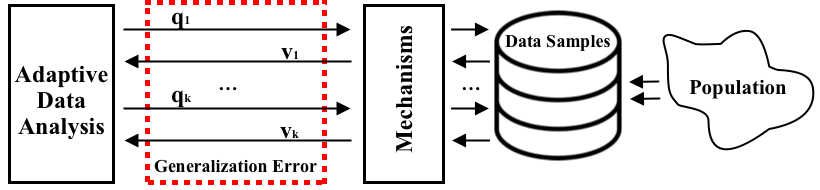
\includegraphics[width=0.7\columnwidth]{figures/data_analysis_model.png}
 \caption{Overview of our Adaptive Data Analysis model.}
 \label{fig:adaptivity-model-overview}
\vspace{-0.5cm}
\end{figure}
This guarantees that the result of the queries generalizes well. 
This approach is described in Figure~\ref{fig:adaptivity-model-overview}, where
I have a population that I am interested in studying, and a dataset containing individual samples from this population. The adaptive data analysis I am interested in running has access to the dataset through queries of some pre-determined family (e.g., statistical or linear queries) mediated by a mechanism. 
This mechanism uses randomization to reduce the generalization error of the queries issued to the data.
This line of work has identified many new algorithmic techniques for ensuring generalization in adaptive data analysis, leading to algorithms with greater statistical power than all previous approaches. 
Common methods proposed by these works include the addition of noise to the result of a query, data splitting, etc. 
Moreover, these works have also identified problematic strategies for adaptive analysis, showing limitations on the statistical power one can hope to achieve. 
Subsequent works have then further extended the methods and techniques in this approach and further extended the theoretical underpinning of this approach, 
e.g.~\cite{dwork2015reusable,dwork2015generalization,BassilyNSSSU16,UllmanSNSS18,FeldmanS17,jung2019new,SteinkeZ20,RogersRSSTW20}.
%

A key development in this line of work is that the best method for ensuring generalization in an adaptive data analysis depends to a large extent on the number of \emph{rounds of adaptivity}, the depth of the chain of queries. 
As an informal example, the program $x \leftarrow \query_1(D);y \leftarrow \query_2(D,x);z \leftarrow \query_3(D,y)$ has three rounds of adaptivity, since $\query_2$ depends on $D$ not only directly because it is one of its input but also via the result of $\query_1$, 
which is also run on $D$, and similarly, $\query_3$ depends on $D$ directly but also via the result of $\query_2$, which in turn depends on the result of $\query_1$. 
The works I discussed above showed that not only does the analysis of the generalization error depend on the number of rounds, 
but knowing the number of rounds allows one to choose methods that lead to the smallest possible generalization error. 

% \mg{Check the following - also the plots need to be on the same scale!}
For example, these works showed that when an adaptive data analysis uses a large number of rounds 
of adaptivity then a low generalization error can be achieved by the mechanism that 
adds Gaussian noise scaled to the number of rounds to each query result.
When instead an adaptive data analysis uses a small number of rounds of adaptivity then a low generalization error can be achieved by using more specialized methods, such as the data splitting mechanism or the reusable holdout technique from~\cite{DworkFHPRR15}.
To better understand this idea, I show in Figure~\ref{fig:generalization_errors} two experiments showcasing these situations. 
More precisely, in Figure~\ref{fig:generalization_errors}(a) shows the results of a real-world analysis
with two rounds of adaptivity. 
This analysis can be seen as a classifier that first runs 500 non-adaptive queries on the first 500 attributes of the data, looking for correlations between the attributes and a label, and then runs one last query which depends on all these correlations. 
Without any mechanism, the generalization error is pretty large, and the lower generalization error is achieved when the data-splitting method is used. 
In Figure~\ref{fig:generalization_errors}(b) shows the results of a specific analysis
with four hundred rounds of adaptivity. 
This analysis can be seen as a classifier that at each step runs an adaptive query based on the result of the previous ones. 
Again, without any mechanism, the generalization error is pretty large, and the lower generalization error is achieved when the Gaussian noise is used. 
{\small
\begin{figure}
\centering
\begin{subfigure}{.48\textwidth}
\begin{centering}
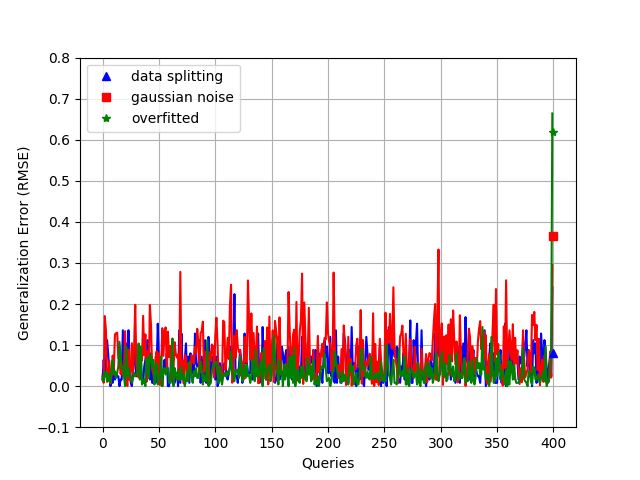
\includegraphics[width=0.9\textwidth]{figures/tworound.png}
\caption{}
\end{centering}
\end{subfigure}
%}
\quad
\begin{subfigure}{.48\textwidth}
\begin{centering}
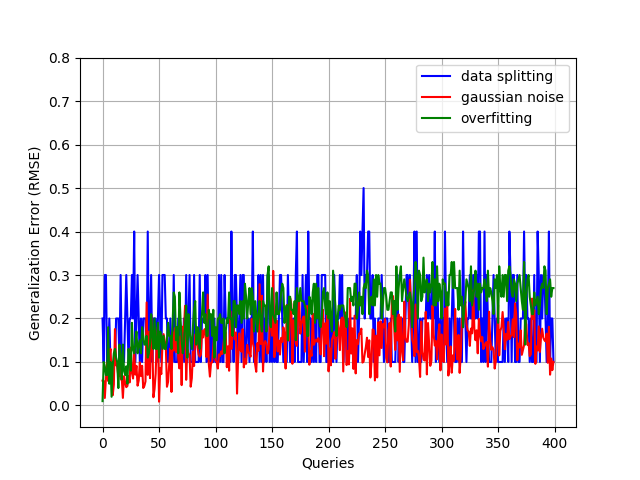
\includegraphics[width=0.9\textwidth]{figures/multipleround.png}
\caption{}
\end{centering}
\end{subfigure}
\vspace{-0.4cm}
 \caption{
 The generalization errors of two adaptive data analysis examples, under different choices of mechanisms.
 (a) Data analysis with adaptivity 2, 
 (b) Data analysis with adaptivity 400. 
}
\label{fig:generalization_errors}
\vspace{-0.5cm}
\end{figure}
}
%gap
This scenario motivates us to explore the design of program analysis techniques that can be used to estimate the number of \emph{rounds of adaptivity} that a program implementing a data analysis can perform. These techniques could be used to help a data analyst in the choice of the mechanism to use,
and they
could ultimately be integrated into a tool for adaptive data analysis such as the \emph{Guess and Check} framework by~\cite{RogersRSSTW20}. 
%

\section{Some Results in Adaptive Data Analysis and Challenges}
\label{sec:adapt-motivation}
\subsection{Some results in Adaptive Data Analysis}
%\wq{I think we can move this subsection into appendix. Maybe just leave theorm 1.2 and 1.3}
%\jl{I don't agree}
In Adaptive Data Analysis an \emph{analyst} is interested in studying some distribution $\dist$ over some domain $\univ$.  Following previous works~\cite{DworkFHPRR15,HardtU14,BassilyNSSSU16}, we focus on the setting where the analyst is interested in answers to \emph{statistical queries} (also known as \emph{linear queries}) over the distribution.  A statistical query is usually defined by some function $\query \from \univ \to [-1,1]$ (often other codomains such as $[0,1]$ or $[-R,+R]$, for some $R$, are considered).  The analyst wants to learn the \emph{population mean}, which (abusing notation) is defined as 
$\query(\dist) = {\sample \sim \dist}{\query(\sample)}$. 
%
We assume that the distribution $\dist$ can only be accessed via a set of \emph{samples} $\sample_1,\dots,\sample_n$ drawn independently and identically distributed (i.i.d.)from $\dist$.  These samples are held by a mechanism $\mech(\sample_1,\dots,\sample_n)$ who receives the query $\query$ and computes an answer 
$\answer \approx \query(\dist)$.
%
The na\"ive way to approximate the population mean is to use the \emph{empirical mean}, which (abusing notation) is defined as 
$\query(\sample_1,\dots,\sample_n) = \frac{1}{n} \sum_{i=1}^{n} \query(X_i)$.
However, the mechanism $M$ can adopt some methods for improving the generalization error $| a- \query(\dist)|$.

In this work we consider analysts that ask a sequence of $k$ queries $\query_1,\dots,\query_k$.  If the queries are all chosen in advance, independently of the answers of each other, then we say they are \emph{non-adaptive}.  If the choice of each query $\query_j$ depend on the prefix $\query_1,\answer_1,\dots,\query_{j-1},\answer_{j-1}$ then they are \emph{fully adaptive}.  An important intermediate notion is \emph{$\qrounds$-round adaptive}, where the sequence can be partitioned into $\qrounds$ batches of non-adaptive queries.  Note that non-adaptive queries are $1$-round and fully adaptive queries are $k$-round adaptive.

We now review what is known about the problem of answering $r$-round adaptive queries.  
\begin{thm}[\cite{BassilyNSSSU16}] 
\label{thm:nonadapt-adapt}
\begin{enumerate}

\item For any distribution $\dist$, and any $k$ \emph{non-adaptive} statistical queries, 
% $$
$
\max_{j=1,\dots,k} | \answer_j - \query_j(\dist) | = O\left( \sqrt{\frac{\log k}{n}}  \right)
% $$
$.
%
\item For any distribution $\dist$, and  any $k$  \emph{$\qrounds$-round adaptive} statistical queries, with $\qrounds \geq 2$, the empirical mean (rounded to an appropriate number of bits of precision)\footnote{With infinite precision even two queries may give unbounded error, when the first query's result encodes the whole data.} satisfies:\\
% $$
$
\max_{j=1,\dots,k} | \answer_j - \query_j(\dist) | = O\left( \sqrt{\frac{k}{n}}  \right)
% $$
$
\end{enumerate}
\end{thm}
In fact, these bounds are tight (up to constant factors) which means that even allowing one extra round of adaptivity leads to an exponential increase in the generalization error, from $\log k$ to $k$.

\cite{DworkFHPRR15} and \cite{BassilyNSSSU16} showed that by using carefully calibrated Gaussian noise in order to limit the dependency of a single query on the specific data instance, one 
can actually achieve much stronger generalization error as a function of the number of queries, specifically.
\begin{thm}[\cite{DworkFHPRR15, BassilyNSSSU16}] \label{thm:gaussiannoise} For any distribution $\dist$, any $k$, any $\qrounds \geq 2$ and any \emph{$\qrounds$-round adaptive} statistical queries, if we answer queries with carefully calibrated Gaussian noise we have:
\begin{center}
  $
\max_{j=1,\dots,k} | \answer_j - \query_j(\dist) | = O\left( \frac{\sqrt[4]{k}}{\sqrt{n}}  \right)
$  
\end{center}
\end{thm}
% Notice that in order to Theorem~\ref{thm:gaussiannoise} has different quantification in that the optimal choice of mechanism depends on the number of queries.  Thus, we need to know the number of queries \emph{a priori} to choose the best mechanism.
More interestingly, \cite{DworkFHPRR15}
also gave a refined bounds that can be achieved with different mechanisms depending on the number of rounds of adaptivity.   \begin{thm}[\cite{DworkFHPRR15}] \label{thm:gaussiannoise2} For any $r$ and $k$, there exists a mechanism such that for any distribution $\dist$, and any $\qrounds \geq 2$ any \emph{$\qrounds$-round adaptive} statistical queries, it satisfies
\begin{center}
  $
\max_{j=1,\dots,k} | \answer_j - \query_j(\dist) | = O\left( \frac{r \sqrt{\log k}}{\sqrt{n}}  \right)
$  
\end{center}
\end{thm}
Notice that Theorem~\ref{thm:gaussiannoise2} has different quantification in that the optimal choice of mechanism depends on the number of queries {and number of rounds of adaptivity}.  This suggests that if one knows a good \emph{a priori upper bound on the number of rounds of adaptivity}, one can choose the appropriate mechanism and get a much better guarantee in terms of generalization error.
As an example, as we can see in Fig.~\ref{fig:generalization_errors}, if we know that an algorithm is two rounds adaptive, we can choose data splitting as {the} mechanism, while if we know that an algorithm has many rounds of adaptivity we can choose Gaussian noise. It is worth to stress that by knowing the number of rounds of adaptivity one can also compute a concrete upper bound on the generalization error of a data analysis. This information allows one to have a quantitative, a priori, estimation of the effectiveness of a data analysis. 
This motivates us to design a static program analysis aimed at giving good \emph{a priori} upper bounds on the number of rounds of adaptivity of a program. 


\subsection{Challenges of Analyzing Adaptivity}
\label{sec:adapt-intro-challenge}
Given the significance of this \emph{adaptivity} quantity in the data analysis area,
I'm motivated to analyze this property.
In order to analyze this property, there are mainly three challenges introduced in Section~\ref{sec:adapt-intro-challenge}.
Then targeting the three challenges, I give a technical overview of the new adaptivity analysis framework
with respect to the limitations of previous works, in Section~\ref{sec:adapt-intro-overview}.

There are mainly three challenges in order to analyze this adaptivity property, 
and the full-spectrum analysis of this property is 
% In this proposal, I will first focus on analyzing 
% this adaptivity property for the program based on solving 
developed w.r.t. the three challenges accordingly.

\begin{enumerate}
 \item
 \textbf{Adaptive Data Analysis Formalization}

The first challenge is \emph{how to define formally} a model for adaptive data analysis which is general enough to support the methods I discussed above and would permit to the formulation of the notion of adaptivity these methods use. 
I take the approach of designing a programming framework for submitting queries to some \emph{mechanism} giving access 
to the data mediated by one of the techniques which are mentioned before, 
including the mechanism of adding Gaussian noise, 
the mechanism that randomly selects a subset of the data, 
and the mechanism that uses the reusable holdout technique, etc. 
In this approach, a program models an \emph{analyst} asking a sequence of queries to the mechanism. 
The mechanism runs the queries on the data applying one of the methods discussed above and returns the result to the program. The program can then use this result to decide which query to run next. 
% Overall, I am interested in controlling the generalization of the results of the queries which are returned by the mechanism, by means of adaptivity. 

% \textbf{Methodology}
% There are previous works from \cite{weihao22} developing language formalizing the adaptive data analysis.
% However, their formalization is limited in the expressiveness largely.
Motivated by this, I present a new while-like language 
named {\tt Query While} language with extensions on query requests in Section~\ref{sec:adapt-language}.

\item 
\textbf{Adaptivity Formalization}

The second challenge is \emph{how to define the adaptivity of a given program}.
Intuitively, a query $Q$ may depend on another query $P$, if there are two values that $P$ can return which affect in different ways the execution of $Q$. 
For example, as shown in \cite{dwork2015reusable}, and as I did in our example in Figure~\ref{fig:generalization_errors}(a), one can design a machine learning algorithm for constructing a classifier that first computes each feature's correlations with the label via a sequence of queries, and then constructs the classifier based on the correlation values. 
If one feature's correlation changes, the classifier depending on features is also affected. 
This notion of dependency builds on the execution trace as a \emph{causal history}. 
In particular, I am interested in the history or provenance of a query up until this is executed, 
% I am not then concerned about how the result is used --- except for 
simultaneously in tracking whether the result of the query may further cause some other query. 
This is because I'm focusing on the generalization error which could be propagated by queries.
% and not their post-processing. % 

To formalize this intuitive \emph{adaptivity} as a quantitative program property, 
I analyze the program's execution based on its semantics
%  develop an execution-based analysis 
in Section~\ref{sec:adapt-exe}.
\item 
\textbf{Adaptivity Estimation}

The third challenge is \emph{how to estimate the adaptivity of a given program}. 
The adaptive data analysis model I consider and our definition of adaptivity suggest that for this task 
I can use a program analysis that is based on some form of dependency analysis.
 This analysis needs to take into consideration:
1) the fact that, in general, a query $Q$ is not a monolithic block but rather it may depend, through the use of variables and values, on other parts of the program. 
Hence, it needs to consider some form of data flow analysis. 
2) the fact that, in general, the decision on whether to run a query or not may depend on some other value. Hence, 
 it needs to consider some form of control flow analysis.
3) the fact that. in general, I am not only interested in whether there is a dependency or not, but in the length of the chain of dependencies. 
Hence, it needs to consider some quantitative information about the program dependencies. % {A quick example is that: I store the result of query $Q_1$ in variable $x$ and use variable $y$ to record the result of query $Q_2$. I want to construct the third query $Q_3$ which relies on the value stored in $x$, let us say, $Q_3$ will ask for the sum of the first column of a table if $x$ is positive and the sum of the second column otherwise. In this situation, I need data flow analysis. On the other hand, if I need the value of $y$ to help us decide whether I should ask $Q_3$, for example, I ask the third query if $y$ is odd, and do not ask if $y$ is even. Naturally, to be able to handle this case, control flow analysis comes into play. Formally speaking, }

To address these considerations and be able to estimate a sound upper bound on the adaptivity of a program, 
I develop a static program analysis in Section~\ref{sec:adapt-static}, named {\THESYSTEM}.
%%%%% To reason about%
\end{enumerate}
% \\
%
\subsection{Technique Overview}
\label{sec:adapt-intro-overview}

\subsubsection{Language Design}
\paragraph*{Research Goal - Adaptive Data Analysis Formalization}
Targeting the first challenge
% --\textbf{Adaptivity Formalization}--
for analyzing the adaptive data analysis, 
the research goal is to develop
an expressive language supporting general adaptive data analysis formally.
% analysis method which can
% % The second challenge is 
% \emph{define} the intuitive \emph{adaptivity} rounds for a given data analysis program formally and accurately.

\paragraph*{Limitations of Previous Works}
There are previous works from \cite{weihao22} developing language formalizing the adaptive data analysis.
However, these language designs are limited in their expressiveness largely.
Most of the general data analyses are not supported by the previous language design.
In Section~\ref{sec:prework-language}, I introduce in detail the previous language design and limitations.
%
\paragraph*{Methodology Overview}
I design a new while-like language 
named {\tt Query While} language in Section~\ref{sec:adapt-language}.
This language is extended from the standard language.
It supports more general data analysis and query requests with more expressive expressions than previous works.

\subsubsection{Adaptivity Formalization}
\label{sec:intro-exe}
% \begin{enumerate}
% \item
% \textbf{Adaptive Data Analysis Formalization}
% The first challenge is \emph{how to define formally} a model for adaptive data analysis which is general enough to support the methods I discussed above and would permit to formulate the notion of adaptivity these methods use. 
% I take the approach of designing a programming framework for submitting queries to some \emph{mechanism} giving access to the data mediated by one of the techniques I mentioned before, e.g., adding Gaussian noise, randomly selecting a subset of the data, using the reusable holdout technique, etc. 
% In this approach, a program models an \emph{analyst} asking a sequence of queries to the mechanism. The mechanism runs the queries on the data applying one of the methods discussed above and returns the result to the program. The program can then use this result to decide which query to run next. 
% % Overall, I'm interested in controlling the generalization of the results of the queries which are returned by the mechanism, by means of adaptivity. 
% \item 
\paragraph{Research Goal - Define the Adaptivity formally}
Targeting the second challenge
% --\textbf{Adaptivity Formalization}--
for analyzing the adaptivity, 
the research goal is to develop an analysis method which can
% The second challenge is 
\emph{define} the intuitive \emph{adaptivity} rounds for a given data analysis program formally and accurately.
% Intuitively, a query $Q$ may depend on another query $P$, if there are two values that $P$ can return which affect in different ways the execution of $Q$. 
% For example, as shown in \cite{dwork2015reusable}, and as I did in our example in Figure~\ref{fig:generalization_errors}(a), one can design a machine learning algorithm for constructing a classifier that first computes each feature's correlations with the label via a sequence of queries, and then constructs the classifier based on the correlation values. 
% If one feature's correlation changes, the classifier depending on features is also affected. 
The intuition behind this \emph{adaptivity} quantity relies on the dependency between the query requests 
executed in the program, and their dependency depth. 
% This notion of dependency builds on the execution trace as a \emph{causal history}. 
Following this intuition, we need to formally define whether there is the dependency between query requests during the program
execution.
%
% And the 
There are different methodologies that can be used to formalize the dependency between two query requests, such as the 
dynamic analysis, execution-based analysis, static analysis, etc.
%
In order to capture the dependency (also the intuitive \emph{adaptivity}) in the most precise way,
% I design the execution-based program analysis method.
I formalize the adaptivity based on the program's execution.
%
% In order to define it in 
% The most precise way to define this dependency is by observing the actual evaluation of these query requests during the 
% program execution.
This execution-based
% program analysis method 
formalization is precise in defining both the dependency relation
% between query requests,
and the intuitive \emph{adaptivity} because it is
% In particular, I'm interested in the history or provenance of a query up until this is executed, I'm not then concerned about how the result is used --- except for tracking whether the result of the query may further cause some other query. 
% Based on this, I design the adaptivity formalization method through the execution-based program analysis techniques.
% These execution-based analysis techniques are 
based on observing the actual evaluation of these query requests during the 
program execution. This is consistent with the intuition of query requests dependency and their dependency depth,
as well as the intuitive
\emph{adaptivity}.
% This is because I focus on the generalization error of queries and not their post-processing. % 
\paragraph{Limitations of Existing Program Semantics and Execution Analysis Techniques}

\begin{itemize}
 \item \textbf{Limitations in Program Semantics and Execution Analysis Area}
 \\
There are many techniques for analyzing a program's semantics or execution, such are program simulation, 
semantics analysis, abstract interpretation, etc., which are widely used in defining
and formalizing the program's properties.
% dependency analysis. 
However, it is not straightforward how to apply them to analyzing and formalizing the \emph{adaptivity}
for adaptive data analysis program.
There are following three limitations among existing execution-based analysis techniques.
\begin{enumerate}
\item The state-of-art dependency relation analysis techniques don't
consider both control influence and value influence. However, both of these
two influences are included in the intuitive query dependency 
in adaptive data analysis programs.
% require
\item In the existing data dependency analysis area, there isn't any technique taking into account
the dependency depth. However, this dependency depth is the key quantity in formalizing the intuitive \emph{adaptivity}.
\item The intuitive \emph{adaptivity} doesn't accumulate linearly through the dependency relation and 
dependency depth. There is only very limited works related to this non-linear quantity property analysis.
This requires us to design new analysis techniques in order to formalize this quantity precisely.
% here isn't any research combining the two pieces of information. No need to mention the adaptivity analysis.
\end{enumerate}
\item \textbf{Limitations in Previous Works on Formalizing Adaptivity} 
\\
There are also previous works on formalizing this quantity from \cite{weihao22}. However, these works
are limited in expressiveness and accuracy significantly.
The \emph{adaptivity} quantities in many general data analysis programs are unable to be defined in the previous \emph{adaptivity} definition.
For the program which is able to be defined,
they cannot give the most precise adaptivity definitions matching the intuitive \emph{adaptivity}.
These previous works and limitations on formalizing the adaptivity are introduced in more detail in Section~\ref{sec:prework-formalization}.
\end{itemize}
%
\paragraph{Methodology Overview}
% To formalize this intuition as a quantitative program property, 
% in Chapter~\ref{ch:dynamic} I develop an execution-based analysis
% % I first consider all the possible evaluations of a program --- I do this by 
% % I use trace semantics recording the execution history of programs on some given input --- and I create a dependency graph, where the dependency between different variables (query is also assigned to a variable) is explicit and track which variable is associated with a query request. 
% % I then enrich this graph with weights describing the maximal number of times each variable is evaluated in a program evaluation starting with an initial state. The adaptivity is then defined as the length of the walk visiting most query-related variables on this graph. 
% % Through two aspects: the execution-based analysis and static-based program analysis.
% % In the execution-based analysis, I will formalize the intuitive notion of \emph{adaptivity} as a quantitative 
% % property of programs. This analysis is developed 
% in three steps through different methodologies in each step as follows,
Given all these limitations and challenges,
to define this intuitive \emph{adaptivity} more precisely as a quantitative program property, 
I give a new adaptivity formalization model by analyzing program's exectuion in Section~\ref{sec:adapt-exe}.
% I first consider all the possible evaluations of a program --- I do this by 
% I use a trace semantics recording the execution history of programs on some given input --- and I create a dependency graph, where the dependency between different variables (query is also assigned to a variable) is explicit and track which variable is associated with a query request. 
% I then enrich this graph with weights describing the maximal number of times each variable is evaluated in a program evaluation starting with an initial state. The adaptivity is then defined as the length of the walk visiting most query-related variables on this graph. 
% Through two aspects: the execution-based analysis and static-based program analysis.
% In the execution-based analysis, I will formalize the intuitive notion of \emph{adaptivity} as a quantitative 
% property of programs. This analysis is developed 
 This execution-based formalization is designed in three steps through different methodologies as follows,
% \begin{enumerate}
% \item The dependency relation between every query, through the methodology of semantic data dependency analysis.
% \\
% Specifically through a trace semantics recording the execution history of programs on some given input
% % --- and I create a dependency graph, 
% the dependency between different variables (query is also assigned to a variable) is explicit and track which variable is associated with a query request. 
% % I then enrich this graph with weights describing the maximal number of times each variable is evaluated in a program evaluation starting with an initial state. The adaptivity is then defined as the length of the walk visiting most query-related variables on this graph. 
% % In the execution-based analysis, I will formalize the intuitive notion of \emph{adaptivity} as a quantitative 
% % property of programs. This analysis is developed 
% % \\
% \item The dependency quantity analysis, through the methodology of execution-based data reachability, bound analysis.
% % \\
% \item The adaptivity quantity analysis, based on the two analysis results above, gives the formal \emph{adaptivity} model 
% for program.
% \\
% Specifically, I create a dependency graph, where the dependency between different variables (query is also assigned to a variable) is explicit and track which variable is associated with a query request. 
% I then enrich this graph with weights describing the maximal number of times each variable is evaluated in a program evaluation starting with an initial state. 
% The adaptivity is then defined as the length of the walk visiting most query-related variables on this graph. 
% \end{enumerate}
\begin{enumerate}
 \item First step is to define the \emph{dependency relation} between every query, 
 through the methodology of semantic data dependency analysis.
 %
 Specifically through a trace semantics recording the execution history of programs on a given input,
 % --- and I create a dependency graph, 
 the dependency between different variables (query is also assigned to a variable) is explicitly tracked and 
 analyzed. This is presented in Section~\ref{sec:dynamic-datadep}.
 % and 
 % which variable is associated with a query request. 
 % I then enrich this graph with weights describing the maximal number of times each variable is evaluated in a program evaluation starting with an initial state. The adaptivity is then defined as the length of the walk visiting most query-related variables on this graph. 
 % In the execution-based analysis, I will formalize the intuitive notion of \emph{adaptivity} as a quantitative 
 % property of programs. This analysis is developed 
 % \\
 \item The second step in Section~\ref{sec:dynamic-reachability} is to analyze the \emph{dependency quantity} 
 % analysis, 
 based on the \emph{dependency relation} above.
 This analysis is developed through the methodology of execution-based reachability bound analysis.
 % \\
 % \item The last step in Section~\ref{sec:dynamic-adapt} is the intuitive \emph{adaptivity} quantity analysis, 
 % according to the two analysis results above, specifically \emph{dependency relation} and \emph{dependency quantity}.
 % This analysis is developed through the formal \emph{adaptivity} definition. \\
 % Specifically, I create a dependency graph, where the dependency between different variables (query is also assigned to a variable) is explicit and track which variable is associated with a query request. 
 % I then enrich this graph with weights describing the maximal number of times each variable is evaluated in a program evaluation starting with an initial state. 
 % The adaptivity is then defined as the length of the walk visiting most query-related variables on this graph. 
 \item The last step is the intuitive \emph{adaptivity} quantity definition, 
 according to the two analysis results above, specifically \emph{dependency relation} and \emph{dependency quantity}.
 This step 
 % is developed through 
 gives the formal \emph{adaptivity} definition. 
 \\
 Specifically, this analysis is developed by creating a dependency graph first. 
 In this graph, the dependency between different variables (query is also assigned to a variable) 
 is explicit and tracks which variable is associated with a query request. 
 This dependency comes from the \emph{dependency relation} from the first step analysis.
 \\
 Then, I enrich this graph with 
 weights describing the maximal number of times each variable is evaluated in a program evaluation starting with an initial state. 
 This weight comes from the \emph{dependency quantity} from the second step analysis results.
 \\
 The adaptivity is then defined as the length of the walk visiting most query-related variables on this graph. 
 \end{enumerate}
 % \item 
\subsubsection{Static Program Analysis}
\label{sec:adapt-intro-static}
% \paragraph{Limitations of Existing Execution-Based Program Analysis Techniques}
%
Though we have the intuitive \emph{Adaptivity} formally and precisely defined through the execution-based program analysis,
it is still not useful enough for programmers.
The weakness of the execution-based formalization comes from its in-efficiency.
It can only give the \emph{Adaptivity} number
after the program is executed multiple times.
When the query requests, the multiple executions consume a large amount of computation and communication resources.
This requires us to develop an efficient analysis method, 
which can provide the programmers with the \emph{Adaptivity} quantity.
Because the static program analysis techniques usually don't require the execution of the program,
they are more efficient than the execution-based formalization.
Motivated by this, we develop a static program analysis framework, named {\THESYSTEM}.
% the through static-based 
% program analysis techniques.
% % In order to provide the programmers with useful information in an efficient way,
% I develop a static program analysis
% to estimate this adaptivity quantity efficiently.
% % , also without lose the usefulness of the information. 
% Through
\paragraph{Research Goal - Adaptivity Estimation}
Targeting on the third challenge
% --\textbf{Adaptivity Formalization}--
for estimating the adaptivity, 
the major research goal is to develop analysis method which can
% The second challenge is 
% give a sound and accurate \emph{upper bound} for the 
provide the programmers with the \emph{adaptivity} quantity
soundly, accurately and
efficiently
% defined 
through static program analysis.
% for a given data analysis program.
% Intuitively, a query $Q$ may depend on another query $P$, if there are two values that $P$ can return which affect in different ways the execution of $Q$. 
% For example, as shown in \cite{dwork2015reusable}, and as I did in our example in Figure~\ref{fig:generalization_errors}(a), one can design a machine learning algorithm for constructing a classifier that first computes each feature's correlations with the label via a sequence of queries, and then constructs the classifier based on the correlation values. 
% If one feature's correlation changes, the classifier depending on features is also affected. 
% The adaptive data analysis model I consider and our definition of adaptivity suggest that for this task I can use a program analysis that is based on some form of dependency analysis. This analysis needs to take into consideration:
There are three sub-research goals in estimating \emph{adaptivity} statically.
Each goal aims to resolve a fact introduced in the \textbf{Adaptivity Estimation} challenge in Section~\ref{sec:adapt-motivation}.
\\
subgoal-1) Designing a data flow analysis algorithm, aims to estimate whether a query may depend on the other queries. 
This analysis needs to consider the monolithic blocks of the program, through the use of variables and values, on other parts of the program.
% the fact that, in general, a query $Q$ is not a monolithic block but rather it may depend, 
% through the use of variables and values, on other parts of the program. 
% Hence, it needs to consider some form of data flow analysis. 
\\
subgoal-2) Integrating the control flow analysis techniques into the static analysis,
 aims to 
capture the query dependency soundly
% in the case
% fact that, in general, the decision on 
% where the dependent query might not be executed under the 
under the control influence.
% of the first query. 
% Hence, 
% it needs to consider some form of control flow analysis.
 \\
subgoal-3) Combining the reachability bound analysis techniques into the static analysis,
% I'm not only interested in whether there is a dependency or not, but in the length of the chain of dependencies. 
% Hence, it needs to consider some 
aims to estimate
% the quantitative information on the query requests dependencies. 
the dependency depth for query requests.
% {A quick example is that: I store the result of query $Q_1$ in variable $x$ and use variable $y$ to record the result of query $Q_2$. I want to construct the third query $Q_3$ which relies on the value stored in $x$, let us say, $Q_3$ will ask for the sum of the first column of a table if $x$ is positive and the sum of the second column otherwise. In this situation, I need data flow analysis. On the other hand, if I need the value of $y$ to help us decide whether I should ask $Q_3$, for example, I ask the third query if $y$ is odd, and do not ask if $y$ is even. Naturally, to be able to handle this case, control flow analysis comes into play. Formally speaking, }
\paragraph{Limitations of Existing Works}
\begin{itemize}
 \item \textbf{Limitations in Static Program Analysis Area}
 \\
 There are many static program analysis techniques, which are widely used in dependency analysis. 
 However, it is not straightforward when applied to adaptivity analysis.
 \begin{enumerate}
 \item To the best of my knowledge,
 existing static dependency analysis techniques do not consider both control influence and value influence.
 But in order to analyze and estimate the \emph{adaptivity} statically, as discussed above, we need to consider both of them.
 \item The existing static analysis techniques in the complexity or resource cost estimation areas,
 cannot give accurate reachability times on programs 
 at every execution location.
 \item Moreover, existing static analysis techniques and their research focus consider
 either only the dependency analysis
 or only the program quantitative property (such as complexity or resource cost),
 but not both of them.
 % No need to mention the adaptivity analysis.
 \end{enumerate}
\item \textbf{Limitations in Previous Works on Estimating Adaptivity}
The previous works from \cite{weihao22}
% ?on estimating this quantity from \cite{weihao22} are limited in the expressiveness, efficiency, and accuracy as well.
% In the previous 
develop program analysis algorithm for estimating the adaptivity.
However, this algorithm is low efficiency, and in-precise. It is not automatic either. 
% The \emph{adaptivity} quantities in many general data analysis programs are unable to be defined in the previous \emph{adaptivity} definition.
% For the program which is able to be defined,
% they cannot give the most precise adaptivity definitions matching the intuitive \emph{adaptivity}.
This analysis algorithm and limitations are introduced with more details in Section~\ref{sec:prework-formalization}.
\end{itemize}

\paragraph{Methodology}
To address these considerations and be able to estimate a sound upper bound on the adaptivity of a program, 
I develop a static program adaptivity analysis framework, named {\THESYSTEM} in Chapter~\ref{sec:adapt-static}.
% which 
% {\THESYSTEM} combines data flow and control flow analysis with reachability bound analysis~\cite{GulwaniZ10}. 
% This new program analysis gives tighter bounds on the adaptivity of a program than the ones one would achieve by directly using the data and control flow analyses or the ones that one would achieve by directly using reachability bound analysis techniques alone. Specifically as follows in the same 3 aspects as the execution-based analysis 
% while through static program analysis techniques, a sound estimated result will be given in each aspect as follows.
This analysis combines data flow and control flow analysis with reachability bound analysis.
% ~\cite{GulwaniZ10}. 
This new program analysis gives tighter bounds on the adaptivity of a program than the ones one would achieve 
by directly using the data and control flow analyses or the ones that one would achieve 
by directly using reachability bound analysis techniques alone. 
% Specifically as follows in the same 
It is developed in 3 aspects similar to the execution-based adaptivity analysis 
while through static program analysis techniques. 
A sound estimated result is given in each part, which is summarized as follows.
\begin{enumerate}
% \item The data dependency relation analysis through the static data flow analysis technique.
% \item The dependency quantity analysis through the static program reachability bound analysis techniques.
% \item The program adaptivity estimation, through newly designed algorithms based on the results estimated above, 
% computing the adaptivity upper bound soundly 
% and accurately.
\item The {\THESYSTEM} analyzes the data \emph{dependency relation} through the static data flow analysis technique in Section~\ref{sec:static-dep}.
This analysis corresponds to the first step in execution-based adaptivity analysis. 
The estimated result produced from 
this step is proved as a sound upper bound for the \emph{dependency relation} defined in the adaptivity formalization model from Section~\ref{sec:dynamic-datadep}.
\item 
% Still , 
Corresponding to the second step in execution-based adaptivity analysis, the \emph{dependency quantity} 
is estimated by {\THESYSTEM} through the static program reachability bound analysis techniques, in Section~\ref{sec:static-quantity}.
% This analysis corresponds to the second step in execution-based adaptivity analysis. 
The estimated result produced from 
this step is proved as a sound upper bound for the \emph{dependency quantity} defined in the adaptivity formalization model.
\item 
% The program estimation, 
% In 
The static program adaptivity analysis in this step
% , specifically estimating 
estimates the \emph{adaptivity} formalized in the third step of adaptivity formalization in Section~\ref{sec:static-adapt}.
% is presented in Section~\ref{sec:static-reachability}.
% the program adaptivity estimation, 
According to the third step of execution-based adaptivity analysis, 
{\THESYSTEM} in this step also constructs a program-based dependence graph for approximating the execution-based dependency graph.
% in Section~\ref{sec:dynamic-adapt}.
Then, based on this graph, {\THESYSTEM} 
% I design an algorithm
% based on the results estimated above, 
% computing 
computes the adaptivity upper bound soundly 
and accurately through a newly designed algorithm.
\end{enumerate}

\section{Overview of {\THESYSTEM} through An Example}
\label{sec:adapt-overview}
{\small
\begin{figure}
\centering
\begin{subfigure}{1.0\textwidth}
\begin{centering}
$
    \begin{array}{l}
    \kw{towRounds(k)} \triangleq \\
           \clabel{ \assign{a}{0}}^{0} ;
            \clabel{\assign{j}{k} }^{1} ;\\
            \ewhile ~ \clabel{j > 0}^{2} ~ \edo ~ 
            \Big(
             \clabel{\assign{x}{\query(\chi[j] \cdot \chi[k])} }^{3}  ; 
             \clabel{\assign{j}{j-1}}^{4} ;
            \clabel{\assign{a}{x + a}}^{5}       \Big);\\
            \clabel{\assign{l}{\query(\chi[k]*a)} }^{6}
        \end{array}
$
\caption{}
\end{centering}
\end{subfigure}
\begin{subfigure}{.5\textwidth}
%}
\qquad
\begin{centering}
\begin{tikzpicture}[scale=\textwidth/15cm,samples=200]
\draw[] (0, 10) circle (0pt) node
{{ $a^0: {}^{\lambda \trace_0. 1}_{0}$}};
\draw[] (0, 7) circle (0pt) node
{\textbf{$x^3: {}^{\lambda \trace_0. \env(\trace_0) k}_{1}$}};
\draw[] (0, 4) circle (0pt) node {{ $a^5: {}^{\lambda \trace_0. \env(\trace_0) k}_{0}$}};
\draw[] (0, 1) circle (0pt) node
{{ $l^6: {}^{\lambda \trace_0. 1}_{1}$}};
% Counter Variables
\draw[] (8, 9) circle (0pt) node {\textbf{$j^1: {}^{\lambda \trace_0. 1}_{0}$}};
\draw[] (8, 6) circle (0pt) node {{ $j^4: {}^{\lambda \trace_0. \env(\trace_0) k}_{0}$}};
%
% Value Dependency Edges:
\draw[ ultra thick, -latex, densely dotted,] (0, 1.5)  -- (0, 3.5) ;
\draw[ ultra thick, -latex, densely dotted,] (0, 4.5)  -- (0, 6.5) ;
\draw[ -latex] (0, 4.5)  to  [out=-230,in=230]  (0, 9.5) ;
\draw[ -Straight Barb] (1.5, 3.8) arc (120:-200:1);
\draw[ -Straight Barb] (9, 6.5) arc (150:-150:1);
\draw[ -latex] (8, 6.5)  -- (8, 8.5) ;
\draw[ -latex] (0, 1.5)  to  [out=-230,in=230]  (0, 9.5) ;
% Control Dependency
\draw[ -latex] (2, 7)  -- (6, 9) ;
\draw[ -latex] (2, 7)  -- (5.5, 6) ;
\draw[ -latex] (2, 4.5)  -- (6, 9) ;
\draw[ -latex] (2, 4.5)  -- (5.5, 6) ;
% Edges Produced By Transitivity
\draw[ -latex] (2, 1)  -- (6, 9) ;
\draw[ -latex] (2, 1)  -- (5.5, 6) ;
\draw[ -latex] (0, 1.5)  to  [out=50,in=-50]  (0, 6.5) ;
\end{tikzpicture}
\caption{}
\end{centering}
\end{subfigure}
   \begin{subfigure}{.45\textwidth}
   \begin{centering}
   \begin{tikzpicture}[scale=\textwidth/15cm,samples=200]
\draw[] (0, 10) circle (0pt) node
{{ $a^0: {}^1_{0}$}};
\draw[] (0, 7) circle (0pt) node
{\textbf{$x^3: {}^{k}_{1}$}};
\draw[] (0, 4) circle (0pt) node
{{ $a^5: {}^{k}_{0}$}};
\draw[] (0, 1) circle (0pt) node
{{ $l^6: {}^{1}_{1}$}};
% Counter Variables
\draw[] (6, 9) circle (0pt) node {\textbf{$j^1: {}^{1}_{0}$}};
\draw[] (6, 6) circle (0pt) node {{ $j^4: {}^{k}_{0}$}};
%
% Value Dependency Edges:
\draw[ ultra thick, -latex, densely dotted,] (0, 1.5)  -- (0, 3.5) ;
\draw[ ultra thick, -latex, densely dotted,] (0, 4.5)  -- 
(0, 6.5) ;
\draw[  -latex] (0, 4.5)  to  [out=-230,in=230]  
(0, 9.5) ;
\draw[  -Straight Barb] (1.5, 3.5) arc (120:-200:1);
\draw[  -Straight Barb] (6.5, 6.5) arc (150:-150:1);
\draw[  -latex] (6, 6.5)  -- (6, 8.5) ;
% Control Dependency
\draw[ -latex] (1.5, 7)  -- (5, 9) ;
\draw[ -latex] (1.5, 4)  -- (5, 9) ;
\draw[ -latex] (1.5, 7)  -- (5, 6) ;
\draw[ -latex] (1.5, 4)  -- (5, 6) ;
\draw[  -latex] (0, 1.5)  to  [out=-230,in=230]  (0, 9.5) ;
% Edges Produced By Transitivity
\draw[ -latex] (2, 1)  -- (5, 9) ;
\draw[ -latex] (2, 1)  -- (5, 6) ;
\draw[ -latex] (0, 1.5)  to  [out=50,in=-50]  (0, 6.5) ;
\end{tikzpicture}
\caption{}
   \end{centering}
   \end{subfigure}
\vspace{-0.4cm}
 \caption{(a) The program $\kw{towRounds(k)}$, an example 
%  of a program 
with two rounds of adaptivity (b) The corresponding semantics-based dependency graph (c) The estimated dependency graph from $\THESYSTEM$.
}
\label{fig:overview-example}
% \vspace{-0.8cm}
\end{figure}
}
We illustrate the key technical components of our framework through a simple adaptive data analysis with two rounds of adaptivity.
In this analysis, an analyst asks $k+1$ queries to a mechanism in two phases.
In the first phase, the analyst asks $k$ queries and stores the answers that are provided by the mechanism. In the second phase, the analyst constructs a new query based on the results of the previous $k$ queries and sends this query to the mechanism. 
The mechanism is abstract here and our goal is to use static analysis to provide an upper bound on adaptivity to help choose the mechanism.
This data analysis assumes that the data domain $\univ$ 
contains at least $k$ numeric attributes 
(every query in the first phase focuses on one), which we index just by natural numbers.
The implementation of this data analysis in the language of {\THESYSTEM} is presented in Fig.~\ref{fig:overview-example}(a).

The {\THESYSTEM} language extends a standard while language\footnote{Programs components are labeled, so that we can uniquely identify every component.} with a query request constructor denoted $\query$. Queries have the form $\query(\qexpr)$, where $\qexpr$ is a special expression 
(see syntax in Section~\ref{sec:language}) representing a function $\from \univ \to U$ on rows.
We use $U$ to denote the codomain of queries and it could be $[-1,1]$, $[0,1]$ or $[-R,+R]$, for some $R$ we consider. This function characterizes the linear query we are interested in running. Indeed, as we discussed in the previous section, linear queries compute the empirical mean of a function on rows --- we use $\chi$ to abstract a possible row in the database.
 As an example, $x \leftarrow \query(\chi[j] \cdot \chi[k])$ computes an approximation, according to the used mechanism, of the empirical mean of the product of the $j^{th}$ attribute and $k^{th}$ attribute, identified by $\chi[j] \cdot \chi[k]$. Notice that we don't materialize the mechanism but we assume that it is implicitly run when we execute the query. 
 In Fig.~\ref{fig:overview-example}(a), the queries inside the while loop correspond to the first phase of the data analysis and compute an approximation of 
the product of the empirical mean of the first $k$ attributes. 
The query outside the loop corresponds to the second phase and computes an approximation of the empirical mean where each record is weighted by the sum of the empirical mean of the first $k$ attributes.


This example is intuitively 2-rounds adaptive since we have two clearly distinguished phases, and the queries that we ask in the first phase do not depend on each other (the query $\chi[j] \cdot \chi[k]$ at line $3$ only relies on the counter $j$ and input $k$), while the last query 
(at line 6) depends on the results of all the previous queries. 
However, capturing this concept formally is surprisingly difficult. The difficulty comes from the fact that a query can depend on the result of another query in multiple ways, by means of data dependency or control flow dependency.
% \mg{this is weaker than it was in the previous submission.}

%%%%%%%%%%%%%%%%%%%%%%%%%%%%%%%%%%%Some details that might be useful when make passes %%%%%%%%%%%%%%%%%
% \jl{ The $\bullet$ stands for no query, for instance, the second event in the trace $(j, 1, \env(\trace)k , \bullet) $ tells us the assignment at line $1$ does not request a query.} \jl{The third event is a testing event corresponding to the guard of the while loop at line $2$. The evaluation of the query request in the second phase is tracked in }
% % \jl{ 
% The $\bullet$ is a default value for non-query event, 
% for instance, the second event in the trace $(j, 1, K , \bullet) $ tells us the assignment at line $1$ does not request a query.
% The third event is a testing event corresponding to the guard of the while loop at line $2$. The evaluation of the query request in the second phase is tracked in 
% % }
\subsubsection{Adaptivity definition}
\label{sec:adaptivity-informal}
%%%%%%%%%%%%%%%%%%%%%%%%%%%%%%%%%%% Details Below that might be useful when make passes %%%%%%%%%%%%%%%%%
% \detailed{To formally define the adaptivity, we build a directed graph representing the possible dependencies between queries of a program and we call this graph: execution-based dependency graph. The vertices represent the assigned program variables and the edges satisfy the dependency relations between vertices.   Fig.~\ref{fig:overview-example}(b) is the execution dependency graph we build based on the "two rounds strategy program" in Fig.~\ref{fig:overview-example}(a). In brief, the graph is built by collecting the assigned variables with labels of the target program as vertices, which are $a^0$, $j^1$,...$a^5$,$l^6$. We check if there is an edge between two vertices by our dependency relation over two labeled variables (defined in Section~\ref{sec:dep_adaptivity} ). This dependency relation relies on the execution of the program recorded by a trace generated by our trace semantics, which is the reason we call this graph "execution-based". 
% Intuitively from Fig.~\ref{fig:overview-example}(a), the query in the second phase (at line 6) depends on the query results in the first phase stored in $a$ at line 5, and the variable $a$ also relies on the queries at line 3. Correspondingly, we have two edges $(l^6, a^5)$ and $(a^5, x^3)$ in our execution-based dependency graph in Fig.~\ref{fig:overview-example}(b). Besides, we also have special edge which is a circle, to track any variable being updated with its previous value recursively. For instance, the counter $j$ and the variable $a$ are updated based on previous values $k$ times in the first phase and we see two circle edges on $a^5$ and $j^4$.}

The central property we are after in this work is the \emph{adaptivity of a program}. We define formally this notion in three steps, which we will describe in details in Section~\ref{sec:adaptivity}. First, we define a notion of dependency, or better \emph{may-dependency}, between variables. To do this we take inspiration from previous works on dependency analysis and information flow control and we say that a variable \emph{may depend} on another one if changing the execution of the latter can affect the execution of the former. 
We can see in Fig.~\ref{fig:overview-example}(a) that the value of the variable $l$, which corresponds to the result of the execution of the query in the second phase (in the command with label 6), is affected by the value of the variable $x$, which corresponds to the result of the execution of the query at line 3 in the first phase, via the variable $a$.
To formally define this notion of dependency, as in information flow control, we use the execution history of programs recorded by a trace semantics (see Definition~\ref{def:var_dep}).
% \mg{Please, double check that I refer to the right definition. }  

Second, we build an annotated weighted directed graph representing the possible dependencies between labeled variables. We call this graph \emph{semantics-based dependency graph} to stress that this graph summarize the dependencies we could see if we knew the overall behavior of the program. 
The vertices of the graph are the assigned program variables with the label of their assignments, edges are pairs of labeled variables which satisfy the dependency relations, weights are functions associated with vertexes and describing the number of times the assignment corresponding to the vertex is executed when the program is run in a given starting state\footnote{In our trace semantics the state is recorded in the trace, so an initial state is actually represented by an initial trace. We will use this terminology in later sections.}, and the annotations, which we call \emph{query annotations}, are bits associated with vertexes and describing if the corresponding assignment comes from a query (1) or not (0).
The \emph{semantics-based dependency graph} of the $\kw{twoRounds(k)}$ program
we gave in Fig.~\ref{fig:overview-example}(a) is described in Fig.~\ref{fig:overview-example}(b) (we use dashed arrows for two edges that will be highlighted in the next step, for the moment these can be considered similar to the other edges---i.e. solid arrows). We have all the variables that are assigned in the program with their labels, and edges representing dependency relations between them. 
For example, we have two edges $(l^6, a^5)$ and $(a^5, x^3)$ describing the dependency between the variables assigned by queries. The vertices $l^6$ and $x^3$ are the only ones with query annotation $1$ (the subscript), since they are the only two variables that are in assignments involving  queries. Notice that the graph contains cycles---in this example it contains two self-loops. These cycles capture the fact that the variables $a^5$ and $j^4$ are updated at every iteration of the loop using their previous value. Cycles are essential to capture mutual dependencies like the ones that are generated in loops. Adaptivity is a quantitative notion, so capturing this form of dependencies is not enough. This is why we also use weights. The weight of a vertex is a function that given an initial state returns a natural number representing 
the number of times the assignment corresponding to a vertex is visited during the program execution starting in this initial state.  
For example, the vertex $l^{6}$ has weight {$\lambda \trace.1$} since for every initial state {$\trace$} the corresponding assignment will be executed one time, the vertex $a^5$ on the other hand has weight {$\lambda \trace. \env(\trace) k$ since the corresponding assignment will be executed a number of times that correspond to the value of $k$ in the initial state $\trace$, and $\env$ is the operator reading value of $k$ from $\trace$.
}

Third, we can finally define adaptivity using the semantics-based dependency graph. We actually define this notion with respect to an initial state $\tau$, since different states can give very different adaptivity.  We consider the longest walk  that visits each vertex $v$ of the semantics-based dependency graph no more than the value that the weight $w_v$ assign to $\tau$, and visits as many query nodes as possible. The number of query nodes visited is the adaptivity of the program with respect to $\tau$.
Looking again at Fig.~\ref{fig:overview-example}(b), and assuming that $\tau(k) \geq 1$, we can see that the 
the walk along the dashed arrows,  $l^{6} \to a^5 \to x^3 $ has two vertices with query annotation $1$, and we cannot find another walk having more than $2$ vertices with query annotation $1$. So the adaptivity of the program in Fig.~\ref{fig:overview-example}(a) with respect to $\tau$ is $2$. If we consider an initial state $\tau$ such that $\tau(k)=0$ we have that the adaptivity with respect to $\tau$ is instead $1$. 

 %%%%%%%%%%%%%%%%%%%%%%%%%%%%%%% Previous Version Above for Reference  %%%%%%%%%%%%%%%%%
To compute statically a sound and accurate upper bound on the \emph{adaptivity} of a program $c$,
we design a program analysis framework named {\THESYSTEM} which we will describe formally in \ref{sec:adapt-static}. 
The structure of {\THESYSTEM} (Fig.~\ref{fig:adaptfun}) reflects in part the definition of adaptivity we discussed in the previous section. Specifically, {\THESYSTEM} is composed by two algorithms (the ones in dashed boxes in the figure), one for building a dependency graph, which we call \emph{estimated dependency graph}, and the other to estimate the adaptivity from this graph.  
The first algorithm, which we will describe formally in Section~\ref{sec:adapt-static}, generates the \emph{estimated dependency graph} using several program analysis techniques. Specifically, {\THESYSTEM} extracts the vertices and the query annotations by looking at the assigned variables of the program, it estimates the edges by using control flow and data flow analysis, and it estimates the weights by using symbolic reachability-bound analysis---weights in this graph are symbolic expressions over input variables. 
% This combined analysis allow us to obtain more accurate upper bounds than what we would obtain by using any of these single analysis technique in isolation.
The second algorithm estimates the longest walk which respect the weights and which visit as many query nodes as possible. 
The two algorithm together gives us an  upper bound on the program's \emph{adaptivity}.

 \begin{figure}
  \centering    
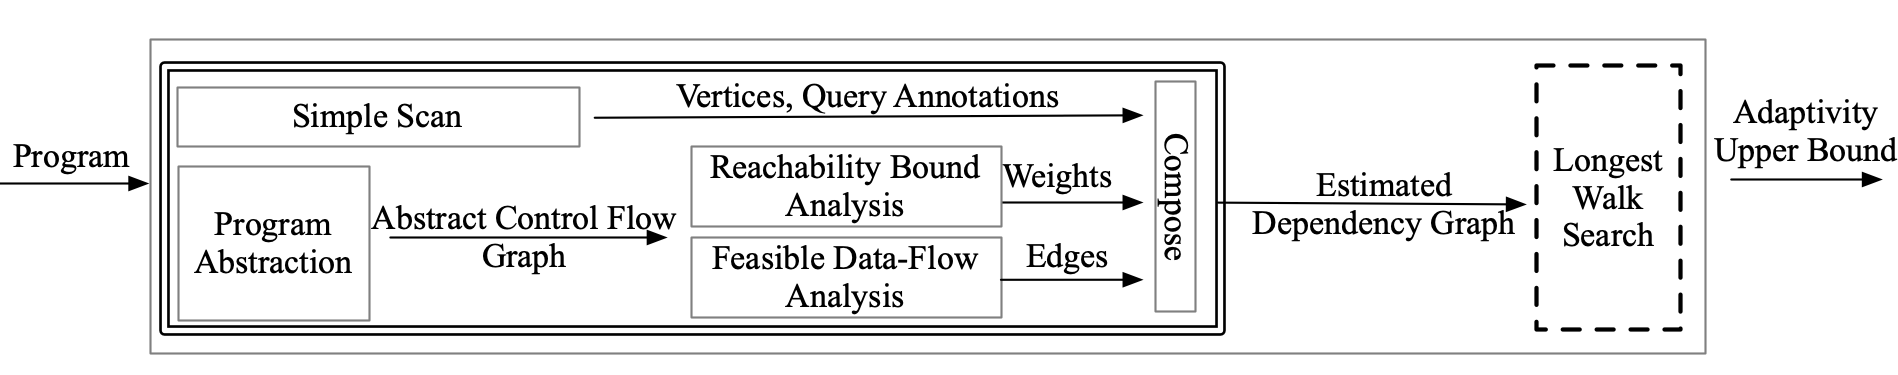
\includegraphics[width=1.0\columnwidth]{adaptfun.png}
  \vspace{-0.8cm}
  \caption{The overview of {\THESYSTEM}}
  \label{fig:adaptfun}
  \vspace{-0.5cm}
\end{figure}

 
%%%%%%%%%%%%%%%%%%%%%%%%%%%%%%%%%%% Details Below that might be useful when others are making passes %%%%%%%%%%%%%%%%%
%   \detailed{Fig.~\ref{fig:overview-example}(c) is the resulting estimated graph of our static analysis algorithm which consumes the program in Fig.~\ref{fig:overview-example}(a).The edges are generated by our graph generation algorithm which combines control flow analysis and data flow analysis, presented in Section~\ref{sec:alg_edgegen}). We can easily see the generated graph in Fig.~\ref{fig:overview-example}(c) is a safe approximation of its execution-based counterpart in Fig.~\ref{fig:overview-example}(b), in the way that we can find a corresponding edge in Fig.~\ref{fig:overview-example}(c) for all the edges in Fig.~\ref{fig:overview-example}(b). We call the weight of every vertex computed by our algorithm as estimated weight,  }
%   estimated by using a reachability-bound estimation algorithm (presented in Section~\ref{sec:alg_weightgen}). \detailed{Different from the execution-based weight $w_1$ or $w_k$ in Fig.~\ref{fig:overview-example}(b) which is a function whose output relies on the initial trace, our estimated weight} can be symbolic and provide a sound upper bound on its execution-based weight of the corresponding vertex in the execution-based dependency graph. For instance, 
%   the estimated weight $k$ of the vertex $x^{3}$ in Fig.~\ref{fig:overview-example}(c) is a sound upper bound on the execution-based weight $w_k$ of vertex $x^{3}$ in Fig.~\ref{fig:overview-example}(b), with the same starting trace $\trace$, $w_k(\trace) \leq\trace(k)$. $\trace(k)$ means getting the value of variable $k$ in the trace $\trace$. The soundness of this step is proved in Theorem~\ref{thm:addweight_soundness}.   
%
We show in Fig.~\ref{fig:overview-example}(c) the estimated dependency graph that our static analysis algorithm returns for the program $\kw{twoRounds(k)}$ in Fig.~\ref{fig:overview-example}(a).
Vertices and query annotations are the same as the ones in Fig.~\ref{fig:overview-example}(b) and they are simply inferred by scanning the program.
As we said before, the edges are estimated using control flow and data flow analysis.
For the $\kw{twoRounds(k)}$ example, every edge in Fig.~\ref{fig:overview-example}(b) is precisely inferred by our combined analysis, this is why Fig.~\ref{fig:overview-example}(c) contains exactly the same edges.
The weight of every vertex is computed using a reachability-bound estimation algorithm which output a symbolic expression over the input variables, in the example only $k$, representing an upper bound on the number of times each assignment is executed.
% \wq{symbolic and provide a sound upper bound on its execution-based weight of the corresponding vertex in the execution-based dependency graph.
% $w_k(\trace) \leq \trace(k)$. $\trace(k)$ means getting the value of variable $k$ in the trace $\trace$. The soundness of this step is proved in Theorem~\ref{thm:addweight_soundness}.}
For example, consider the vertex $x^{3}$, its weight is $k$ and this provides an upper bound on the values returned by the weight function $\lambda \trace. \rho(\trace)k$ associated with vertex $x^{3}$ in Fig.~\ref{fig:overview-example}(b) for any initial state. 
% Indeed, 
% for any initial trace $\trace_0$, when $w_{x^{3}}(\trace_0)$ executes the program and counts the
% execution times of command $3$,
% we expect that this counts is at most the the loop iterations, i.e. $k$'s initial value from $\trace_0$.

The algorithm searching for the longest walk first finds a path $l^6:{}^1_1 \to a^5: {}^k_1 \to x^3: {}^k_1$, and then constructs a walk based on this path. Every vertex on this walk is visited once, and the number of vertices with query annotation $1$ in this walk is $2$, which is the upper bound we expect.
{It is worth to note here that $x^3$ and $a^5$ can only be visited once because there isn't an edge to go back to them, even though they both have the weight $k$}.
In this sense, instead of simply computing the weighted length of this path ($2k+1$) as adaptivity $\pathsearch$ computes the upper bound $2$. Note that $2$ is not always tight, for example when $k = 0$.


\section{Outline and Contributions}
\label{sec:adapt-outline}
Two main parts :
\\
the first part focus on solving the Reachability-Bound Problem through static program analysis.
\\
The second part focus on analyzing the adaptivity -- a quantity property -- for programs in data analysis area,
through both the  static program analysis techniques and execution-based analysis techniques.
\begin{enumerate}
    \item \redd{PART \romannum{1} \quad  REACHABILITY BOUND ANALYSIS}

        \paragraph{Chapter~\ref{sec:reachability-intro}} Introduction with sections:
        
        Section~\ref{sec:reachability-background}: {Reachability Bound Problem}
        
        Section~\ref{sec:reachability-motivation}: {Motivation and Overview}
        
        Section~\ref{sec:reachability-outline}: {Chapter Outline}

        \paragraph{Chapter~\ref{sec:reachability-analysis}}: {Path-Sensitive Reachability Bound Analysis}

        Section~{\ref{sec:language}}{{Program Model}}
        1. {Language}
        2. {Trace-Based Operational Semantics}
        3. {{Reachability Bound Formalization}}

        % % % % 
        Section~\ref{sec:reachability-program_refine}: {Program Abstraction and Refinement}
        % \subsection{Constraint Program Refinement}

        Section~\ref{sec:reachability-analysis}: {Path Sensitive Reachability Bound Analysis}
        1.{Outside-In Algorithm}
        2. {Inside-Out Algorithm}

        \paragraph{Chapter~{\ref{sec:reachability-example}}}: {Examples and Experimental Results}

    \item \redd{PART \romannum{2} \quad  PROGRAM ANALYSIS FRAMEWORK FOR ADAPTIVE DATA ANALYSIS}
    shows the work on the program analysis algorithms to study the adaptivity of the adaptive data analysis program.    

    \paragraph{Chapter~\ref{sec:adapt-intro}} gives the introduction of adaptive data analysis in Section~\ref{sec:adapt-background} and the challenges (Section~\ref{sec:adapt-motivation}) we face to obtain the adaptivity to control the generalization error of an adaptive data analysis program, with an outline of this part in Section~\ref{sec:adapt-outline}.
    
    \paragraph{Chapter~\ref{sec:prework}} introduces the previous works on adaptivity analysis.
    It contains a short summary of the language designs in Section~\ref{sec:prework-language} 
    the adaptivity formalization through program analysis over the trace-based operational semantics (Section~\ref{sec:prework-formalization}),
    and previous program analysis algorithm that is used to estimate the adaptivity of the data analysis programs 
    in Section~\ref{sec:prework-static}
    % (Section~\ref{sec:adapt-ve}, Section~\ref{sec:adapt-matrix}). 
    Their algorithm first introduces the SSA version of the loop language
    % (Section~\ref{sec:adapt-syntax-ssa-loop})
     to enable an easier analysis over adaptivity by an easier tracking of dependency relations between variables based of the limitation of direct analysis over the loop language
    %   is covered in Section~\ref{sec:adapt-limit}. The transformation from the loop language to the SSA loop language is presented in Section~\ref{sec:adapt-transformation}.
    Following with a three-step algorithm, which constructs a data control dependency graph, and add weights to the graph. The adaptivity is estimated by the weight of the path with the highest weight.
    % we use to express data analysis programs, and shows the definition of adaptivity from a trace-based operational semantics in Section~\ref{sec:adapt-os}.


    \paragraph*{Chapter~\ref{sec:adapt-analysis}} presents the new adaptivity analysis framework with significant improvement in three sections.
    \\
    Section~\ref{sec:adapt-language} present a more expressive while-like language than previous works. This extended language supports more general adadptive data analysis.
    \\
    Section~\ref{sec:adapt-exe} presents the new definition for
    %   develops an execution-based analysis method which can
    % The second challenge is 
    % \emph{define} 
    the intuitive \emph{adaptivity} rounds for a given data analysis program through a formal semantics model.
    % Intuitively, a query $Q$ may depend on another query $P$, if there are two values that $P$ can return which affect
    It is defined in three steps. 
    The Section~\ref{sec:dynamic-datadep} reasons the \emph{dependency relation} between every query, 
    through the methodology of semantic data dependency analysis.
    In Section~\ref{sec:dynamic-reachability}, it analyzes the \emph{dependency quantity} 
    %  analysis, 
    based on the \emph{dependency relation} above.
    This step is developed through the methodology of execution-based reachability bound analysis.
    The last step in Section~\ref{sec:dynamic-adapt} is the intuitive \emph{adaptivity} quantity analysis, 
   according to the two definitions above, specifically \emph{dependency relation} and \emph{dependency quantity}.
    This step 
  %  is developed through 
    gives the formal \emph{adaptivity} definition. 
    \\
    Section~\ref{sec:adapt-static} develops an improved static program adaptivity analysis framework, named {\THESYSTEM}.
    This analysis combines data flow and control flow analysis with reachability bound analysis.
    % Specifically as follows in the same 
    It is developed in 3 aspects similar to the execution-based adaptivity analysis 
    while through static program analysis techniques. 
    The {\THESYSTEM} analyzes the data \emph{dependency relation} through the static data flow analysis technique
    in Section~\ref{sec:static-dep}.
    In Section~\ref{sec:static-quantity}, the \emph{dependency quantity} 
    is estimated by {\THESYSTEM} through the static program reachability bound analysis techniques corresponding to the second step in execution-based adaptivity analysis.
    In the last step, {\THESYSTEM}
    % , specifically estimating 
    estimates the \emph{adaptivity} formalized through execution-based analysis in Section~\ref{sec:static-adapt},
    %  is presented in Section~\ref{sec:static-reachability}.
    % the program adaptivity estimation, 
    % According to the third step of execution-based adaptivity analysis, 
    % {\THESYSTEM} in this step also 
    via constructing a program-based dependence graph for approximating the execution-based dependency graph.
    

    \paragraph{Chapter~\ref{sec:adapt-implementation}} presents five manual examples demonstrating this framework in Section~\ref{sec:adapt-example},
    and the experimental results on some real world data analysis algorithms in Section~\ref{sec:adapt-eval}.
    % It includes a variant of two round data analysis algorithm, an adaptive multiple rounds data analysis algorithm and an example showing the over-approximate of our approach (Section~\ref{sec:adapt-example-over}). 
    
    \paragraph{Chapter~\ref{sec:adapt-relatedwork}} discusses the related works from three perspectives:
    Static program analysis (Section~\ref{sec:relatedwork-static}), dynamic program analysis (Section~\ref{sec:relatedwork-exe}) and generalization in adaptive data analysis (Section~\ref{sec:relatedwork-adapt}).  

    \item \redd{PART \romannum{3} \quad  Conclusion and Future Works}
    \paragraph*{Chapter~\ref{sec:conclusion}}
    Concludes the two works, i.e., Program Analysis Framework for Adaptive Data Analysis
    and the Path-Sensitive Reachability-Bound Analysis of this dissertation.

    \paragraph*{Chapter~\ref{sec:future}}
    Discusses two future directions.
    The first direction based on studying the reachability quantitative properties,
   is {The Program Non-Monotonic Quantitative Property Analysis} in Section~\ref{sec:future-cost}.
   The second direction combines with the research in complexity theory area, I plan to reason
   about the Solving the CFL Reachability Problem in Section~\ref{sec:future-cfl}.
    % % relative cost and adaptivity.
    % \\
    % \textbf{Program Non-Monotonic Resource Cost Analysis}
    %     Moving towards the area of general program resource cost analysis,
    %     % Then, motivated by the two following aspects, 
    %     there are two interesting observations as follows.
    %     % I'm interested 
    %     These two observations motivated me in 
    %     % improving the accuracy of the program's general resource cost analysis
    %     improving the accuracy of the program's general resource cost analysis
    %     by generalizing this full-spectrum \emph{adaptivity} analysis.
    %     \begin{itemize}
    %     \item Firstly, in a traditional program's resource cost analysis,
    %     There are two categories of program cost analysis, type-system based and data-flow/control-flow analysis based. 
    %     In the type-system design-based works, they \cite{GustafssonEL05} and \cite{hoffmann_jost_2022}, explicit abstraction or data structure de-allocation in order to save or reduce the cost.
        
    %     Both of the
    %     works in these two areas fail to recognize the case where program resource consumption is decreased implicitly.
    %     \item The resource consumption during the program 
    %     execution increases and particularly decreases implicitly in the same way as the program's adaptivity. 
    %     This is explained in detail through an example in Section~\ref*{sec:generalcost-backgroung}.
    %     \end{itemize}
    %     Based on the observations above, in Chapter~\ref{ch:generalization},
    %     %  Based on the observations above, and through the generalized \emph{adaptivity} analysis framework.
    %     %  I will give
    %     %  a more accurate resource cost estimation by taking the program's implicit resource cost into consideration, compared 
    %     %  to the worst-case cost analysis in the traditional way.
    %     I develop
    %     an accurate program general resource cost analysis framework through generalizing my full-spectrum \emph{adaptivity} analysis.
    %     This framework can give more accurate cost bound than traditional worst-case resource cost estimation methods,
    %     by taking the program's implicit resource cost into consideration.
    %         \\
    %         \textbf{Solving the CFL Reachability Problem}
    %     Still in the area of general program resource cost analysis,
    %     the traditional methodology of performing data flow and control analysis and 
    %     computing the program resource cost is
    %     % Finally, based on the study on the traditional way of performing data flow and control analysis,
    %     to reduce the analysis problem into the CFL-reachability problems.
    %     % Finally, based on the study on the traditional way of performing data flow and control analysis,
    %     According to this, 
    %     I identify x
    %     % the similarity between the traditional way of performing data flow and control analysis and the 
    %     the similarities between the traditional way of estimating the program resource cost and 
    %     the adaptivity.
    %     %  Specifically, I identify the similarity between 
    %     %  solving the feasible path problem in the analysis by reducing 
    %     Specifically, there are similarities between solving the CFL-reachability problems they reduced to,
    %     %  CFL-reachability problems,
    %     and the way of computing the adaptivity in 
    %     %  my static analysis framework.
    %     the third step of $\THESYSTEM$.
    %     Motivated by this, 
    %     % I'm Interested
    %     % the, There are similarities between
    %     % solving the data flow problem by reducing to CFL-reachability problem,
    %     % resource analysis through reducing to CFL-reachability problem, 
    %     I'm interested in showing that
    %     CFL-reachability problems can be solved by reducing to my adaptivity analysis framework.

    \item \redd{PART \romannum{4} \quad  APPENDIX}
    The Appendix contains the complete examples, theorems and proofs for the two works of this dissertation.
\end{enumerate}

\textbf{Previous Published Materials}

\chapter{Previous Works on Adaptivity Analysis}
\label{sec:prework}
This chapter introduces the previous works on analyzing the adaptivity property
for adaptive data analysis and the limitation analysis.
There are mainly three parts in previous works.
Each of them focus on solving one of the challenges introduced above in analyzing the adaptivity.
In Section~\ref{sec:prework-language}, I introduce the previous language design, which aims to formalize
the adaptive data analysis program and solve the first challenge.
Section~\ref{sec:prework-formalization} summarizes the previous works
on defining this intuitive \emph{adaptivity} quantity through a formal model,
targeting on the second challenge.
Then Section~\ref{sec:prework-static} includes a summary of previous works on estimating
their formalized \emph{adaptivity} and the limitations.

%
\section{The Language Design}
\label{sec:prework-language}
Previous works formalized the adaptive data analysis into a while-like language named loop language with  limited expressiveness.
It is presented in {Thesis~\cite{weihao22}}.
\subsection*{Syntax}
Figure~\ref{fig:prework_syntax} is a selection of the syntax from their loop language.
{\small
\begin{figure}
\[
\begin{array}{llll}
    % \mbox{Values } & v & ::= & n \sep \etrue \sep \efalse \sep \chi \sep [] ~|~ [v, \dots, v] ~|~ \chi[v] \\
 \mbox{Arithmetic Operators} & \oplus_a & ::= & + ~|~ - ~|~ \times 
%
~|~ \div \\  
  \mbox{Boolean Operators} & \oplus_b & ::= & \lor ~|~ \land ~|~ \neg\\
  %
   \mbox{Relational Operators} & \sim & ::= & < ~|~ \leq ~|~ == \\  
%  \mbox{Label} & l & := & \mathbb{N} \\ 
%  \mbox{Loop Maps} & w & \in & \mbox{Label} \times \mathbb{N} \\
\mbox{Arithmetic Expressions} & \aexpr & ::= & 
	%
	n ~|~ x ~|~ \aexpr \oplus_a \aexpr  \\
% 	\sep \pi (l , \aexpr, \aexpr) \\
    %
\mbox{Boolean Expressions} & \bexpr & ::= & 
	%
	\etrue ~|~ \efalse  ~|~ \neg \bexpr
	 ~|~ \bexpr \oplus_b \bexpr
	%
	~|~ \aexpr \sim \aexpr \\
\mbox{Expressions} & \expr & ::= & \aexpr ~|~ \bexpr ~|~ [] ~|~ [\expr, \dots, \expr] \\	
\mbox{Values} & v & ::= & n ~|~ \etrue ~|~ \efalse ~|~ [] ~|~ [v, \dots, v] \\
\mbox{Query expressions} & \expr_q & ::= & \aexpr ~|~ \chi ~|~ \chi[\aexpr] ~|~ \expr_q \oplus_a \expr_q \\
\mbox{Query Values} & v_q & ::= & n ~|~ \chi ~|~ \chi[n] ~|~ v_q \oplus_a  v_q \\
% \mbox{Labelled commands} & c & ::= & 
% [\assign x \expr]^{l} ~|~  [\assign x q(e_q)]^{l}
%  ~|~  \eloop ~ [\aexpr]^{l} ~ \edo ~ c  ~|~ c;c \\
%  & & & ~|~ \eif([\bexpr]^l, c, c) 	 ~|~ [\eskip]^{l} \\
\mbox{Commands} & c & ::= &  \eskip  ~|~  \assign x \expr ~|~  \assign{x}{ q(\expr_q)}
%
~|~ \eloop ~ \aexpr  ~ \edo ~ c  \\ &&& ~|~ c;c  ~|~ \eif(\bexpr, c, c)
\end{array}
\]
 \caption{Syntax of loop language.}
    \label{fig:prework_syntax}
\end{figure}
}
The expressions can be arithmetic expressions, boolean expressions or query expression.
The arithmetic expressions boolean expressions are standard.
They extend the expression with the query expression in order to support the query requests in the data analysis.
The special variable $\chi$ represents a row of the database,
and access to values at a certain index in $\chi$, as $\chi[\aexpr]$.
But it neither  support while loop with non-deterministic iterations, nor any user input.
%
\subsection*{Trace-Based Operational Semantics}
The previous operational semantics is defined based on labeled command and trace with some special operators.
Below is a summary of their designs.
\paragraph*{Labeled Commands}
They first annotate each command with a label $l$,
a natural number standing for the line of code where the command appears.
They associate the label $l$ to the conditional predicate $\bexpr$ in the if statement,
and to the loop counter $\aexpr$ in the loop statement.
\[
\begin{array}{llll}
     \mbox{Labeled commands} & c & ::= &   [\assign x \expr]^{l} ~|~  [\assign x q(e_q)]^{l}
 ~|~  \eloop ~ [\aexpr]^{l} ~ \edo ~ c  ~|~ c;c \\
 & & & ~|~ \eif([\bexpr]^l, c, c) 	 ~|~ [\eskip]^{l} \\
\end{array}
\]
% Each command is now labeled 
\paragraph*{Loop Map}
Then, they have the Loop map, which is a map from the label $l$ to the iteration number $n$.
%   Because statements in the loop share the same line number,  varied iterations , the label $l$ is not enough to distinguish statements.
  A mapping $[k \to n]$ gives accurate information on which loop a statement is in by its key $k$ (label at loop counter),
  and which iteration $n$ the statement belongs to.
  % For example, the loop map $w=[3:1, 4:2]$ indicates that the statement is currently in a nested loop, the outer loop starting from label $3$ and in its first iteration, the statement is now in the inner loop starting from label $4$ and in the second iteration. We use $\emptyset$ to represent an empty map, indicating the statement is not in any loop.
\[
\begin{array}{llll}
 \mbox{Loop Map} & w & \in & \mbox{Label} \to \mathbb{N} \\
\mbox{Annotated Query} & \mathcal{AQ}  & ::= & \{ q(v_q)^{(l,w)}  \} \\
\end{array}
\begin{array}{llll}
    \mbox{Memory} & m & ::= & [] ~|~ m[x \to v] \\
\mbox{Trace} & t & ::= & [] ~|~ q(v_q)^{(l, w) } :: t \\
\end{array}
\]
%  Then, they have the Loop map, which is a map from the label $l$ to the iteration number $n$.
% %   Because statements in the loop share the same line number,  varied iterations , the label $l$ is not enough to distinguish statements.
%   A mapping $[k \to n]$ gives accurate information on which loop a statement is in by its key $k$ (label at loop counter),
%   and which iteration $n$ the statement belongs to.
%   % For example, the loop map $w=[3:1, 4:2]$ indicates that the statement is currently in a nested loop, the outer loop starting from label $3$ and in its first iteration, the statement is now in the inner loop starting from label $4$ and in the second iteration. We use $\emptyset$ to represent an empty map, indicating the statement is not in any loop.

 \paragraph*{Annotated Query} 
 They 
distinctively design the annotated query, in order to analyze the relation between queries. This is a key extension for analyzing the \emph{adaptivity}
Through this annotation, queries can be uniquely annotated as $\mathcal{AQ}$,
  and the annotation $(l,w)$ considers the location of the query
  by line number $l$ and which iteration the query is at when it appears in a loop statement, specified by $w$.
  %% trace
\paragraph{Trace} 
A trace $t$ is a list of annotated queries accumulated along with the execution of the program. 
%   A trace can be regarded as the program history, where this history 
  It consists of the queries asked by the analyst during the execution of the program,
%   We 
collected through
  a trace-based small-step operational semantics based on transitions of the form $ \config{m,c, t, w} \to \config{m', \eskip, t', w'} $.
  % \paragraph{Memory}
  % The memory in their language is standard, which is a map from variables to values.
  \paragraph*{Operational Semantics Rules}
Figure~\ref{fig:evaluation} is a selection of rules of their trace-based operational semantics from {Thesis~\cite{weihao22}}.
Only the rules related to query requests and the while loop evaluations are selected here.
The rule $\textbf{l-query-e}$ evaluates the argument $\expr_q$ of a query request $q(\expr_q)$ using the query evaluation $\qarrow$.
When the query expression is in the normal form, this query will be answered.
The rule $\textbf{l-query-v}$ modifies the starting memory $m$ to $m[v_q/x]$ using the answer $v$ of the query $q(v_q)$ from the mechanism, with the trace expanded by appending the query $q(v_q)$ with the current annotation $(l,w)$.
The rule for assignment is standard and the trace remains unchanged.
The sequence rule keeps tracking the modification of the trace, and the evaluation rule for if conditional goes into one branch based on the result of the conditional predicate $\bexpr$. 
The rule \textbf{l-loop-a} first evaluates the loop counter $\aexpr$, when the loop counter is a number, then the evaluation will start to execute the loop body.
The rules for loop modify the loop map $w$. In the rule $\textbf{l-loop}$, the loop map $w$ is updated by $w + l$ because the execution goes into another iteration when the condition $v_N >0$ is satisfied.
% When $v_N$ reaches $0$, the loop exits and the loop map $w$ eliminates the label $l$ of this loop statement by $w \setminus l$ in the rule $\textbf{l-loop-exit}$. 
% 
\begin{figure}
{\footnotesize
  \begin{mathpar}
  % \boxed{ \config{m, c, t,w} \xrightarrow{} \config{m', c',  t', w'} \; }
  % \\
  % \inferrule
  % {
  %  \config{m, \expr } \xrightarrow{}  \config{m, \expr' }
  % }
  % {
  % \config{m, [\assign x \expr]^{l},  t,w} \xrightarrow{} \config{m, [\assign x \expr']^{l}, t,w}
  % }
  % ~\textbf{l-assn1}
  % \and
  % %
  % \inferrule
  % {
  % }
  % {
  % \config{m, [\assign x v]^{l},  t,w} \xrightarrow{} \config{m[v/x], [\eskip]^{l}, t,w}
  % }
  % ~\textbf{l-assn2}
  % %
  % \and
  {\inferrule
  {
    \config{m, \aexpr} \aarrow \config{m, \aexpr'}
  }
  {
  \config{m, \eloop ~ [\aexpr]^{l}  ~ \edo ~ c ,  t, w }
  \xrightarrow{} \config{m, \eloop ~ [\aexpr']^{l} ~ \edo ~ c ,  t, (w + l) }
  }
  ~\textbf{l-loop-a}
  }
  %
  \and
  %
  {\inferrule
  {
    \valr_N > 0
  }
  {
  \config{m, \eloop ~ [\valr_N]^{l}  ~ \edo ~ c ,  t, w }
  \xrightarrow{} \config{m, c ;  \eloop ~ [(\valr_N-1)]^{l} ~ \edo ~ c ,  t, (w + l) }
  }
  ~\textbf{l-loop}
  }
  %
  % \and
  % %
  % {
  % \inferrule
  % {
  %   \valr_N = 0
  % }
  % {
  % \config{m,  \eloop ~ [\valr_N]^{l} ~ \edo ~ c  ,  t, w }
  % \xrightarrow{} \config{m, [\eskip]^{l} ,  t, (w \setminus l) }
  % }
  % ~\textbf{l-loop-exit}
  % }
  %
  \and
  % {  Memory \times Com  \times Trace \times WhileMap \Rightarrow^{} Memory \times Com  \times Trace \times WhileMap}
  \inferrule
  {
  \config{m,\expr_q} \qarrow \config{m,\expr_q'}
  }
  {
  \config{m, [\assign{x}{q(\expr_q)}]^l, t, w} \xrightarrow{}  \config{m, [\assign{x}{q(\expr_q')}]^l, t, w}
  }
  ~\textbf{l-query-e}
  \and
  \inferrule
  {
  q(v_q) = v
  }
  {
  \config{m, [\assign{x}{q(v_q)}]^l, t, w} \xrightarrow{} \config{m[ v/ x], \eskip,  t \mathrel{++} [q(v_q)^{(l,w )}],w }
  }
  ~\textbf{l-query-v}
  %
  \and
  %
  %
  % \inferrule
  % {
  % \config{m, c_1,  t,w} \xrightarrow{} \config{m', c_1',  t',w'}
  % }
  % {
  % \config{m, c_1; c_2,  t,w} \xrightarrow{} \config{m', c_1'; c_2, t',w'}
  % }
  % ~\textbf{l-seq1}
  % %
  % \and
  % %
  % \inferrule
  % {
  % }
  % {
  % \config{m, [\eskip]^{l} ; c_2,  t,w} \xrightarrow{} \config{m, c_2,  t,w}
  % }
  % ~\textbf{l-seq2}
  % %
  % %
  % \and
  % %
  % \inferrule
  % {
  % \config{ m, \bexpr} \barrow \bexpr'
  % }
  % {
  % \config{m, \eif([\bexpr]^{l}, c_1, c_2),  t,w} 
  % \xrightarrow{} \config{m,  \eif([\bexpr']^{l}, c_1, c_2),  t,w}
  % }
  % ~\textbf{l-if}
  % %
  % \and
  %
  % \inferrule
  % {
  % }
  % {
  % \config{m, \eif([\etrue]^{l}, c_1, c_2),t,w} 
  % \xrightarrow{} \config{m, c_1,  t,w}
  % }
  % ~\textbf{l-if-t}
  % \and
  % %
  % \inferrule
  % {
  % }
  % {
  % \config{m,  \eif([\efalse]^{l}, c_1, c_2),  t,w} 
  % \xrightarrow{} \config{m, c_2,  t,w}
  % }
  % ~\textbf{l-if-f}
  %
  % %
  %
  \end{mathpar}
  }
        \caption{Trace-based operational semantics of loop language.}
        \label{fig:evaluation}
    \end{figure}
    %
    % explanation of rules
 \highlight{
\paragraph*{Limitations of The Trace-Based Operational Semantics}
This operational semantics is limited in the following aspects:
\begin{itemize}
 \item \textbf{Expressiveness Limitation}
 \\
 The operational-semantics causes a similar limitation as their syntax.
 The loop iteration number can only be a constant number or an arithmetic expression evaluated to a nature number.
 This is caused by their operational semantics rule design, trace design, and their annotated query design.
 In the rule \rname{l-loop}, a nature number $v_N$ is required on the premise of tracking the iteration times.
 This requires that the loop iteration number has to be a nature number or evaluated to a nature number in advance to execute the loop.
 Then in their trace and annotated query design,
 % generated through the operational semantics rules.
 the trace tracks the annotated query, which requires an integer annotation explicitly indicating the iteration number of the loop.
 % annotatation of the the query request executed in the program
 % with integer indicating the while loops. 
 \\
 For example, in the following program with a simple while loop,
 \[
 {\assign{x}{20}};
 \assign{y}{100};
 \ewhile (x < y) \edo 
 \{
 \assign{x}{x + 1};
 \assign{y}{y - 2};
 \}\}
 \] 
 the number of iterations cannot be evaluated to a nature number in advance of entering this loop. 
 The iteration number is only
 able to be decided during executing this while loop body.
 This program represents a class of data analysis programs with non-constant loop iterations
 which is very common in data analysis. However, it isn't supported by their design.
 \item \textbf{Accuracy Limitation}
 \\
 This operational semantics design causes in-precision in formalizing the \emph{adaptivity}.
 Because there is information loss in their trace generated through the operational semantic rules.
 The trace only tracks the query requests. This lost the information of the variables
 which are assigned by query values even if they are not assigned by query requests. However, these variables
 are critical in analyzing the \emph{adaptivity}.
 This will be analyzed in detail in the limitation in Section~\ref{sec:prework-formalization}.
 \item \textbf{Efficiency Limitation}
 \\
 There are four components in their configuration in order to evaluate the program. 
 The update operations for this quadruple configuration are low-efficient, especially the update operation of the while map.
\end{itemize}
}   
%
\section{The Adaptivity Formalization}
\label{sec:prework-formalization}
The previous works on formalizing the adaptivity is through a query-based dependency graph.
Below is a summary of their query-based dependency graph construction and adaptivity formal definition, followed
by the weaknesses of this formalization method.
\subsection*{Query-Based Dependency Graph}
They build their dependency graph over annotated queries, in order to construct the edge between queries for this graph, they first
define a query \emph{May-Dependency} relation. Below is a summary of this definition from
% Below is the formal definition of query may dependency based on their trace-based operational semantics 
from Thesis~\cite{weihao22}.
The notations $\in_q$ and $\not\in_q$ a query belongs to the trace or not respectively, with the full details in Thesis~\cite{weihao22}.
\begin{defn}[Query may dependency]
One query $q({v_q}_1)$ may depend on another query $q({v_q}_2)$ in a program $c$, with a starting loop maps $w$, a starting memory $m$, hidden database $D$, denoted as \\
$\mathsf{DEP}(q({v_q}_1)^{(l_1, w_1)}, q({v_q}_2)^{(l_2, w_2)}, c,w, m, D)$ is defined below. 
\[
  {\footnotesize
\begin{array}{l}
\forall  t. \exists m_1,m_3,t_1,t_3,c_2.\\
  \left (\begin{array}{l}   
\config{m, c,  t,w} \rightarrow^{*} \config{m_1, [\assign{x}{q({v_q}_1)}]^{l_1} ; c_2,
  t_1,w_1} \rightarrow \\ \config{m_1[q({v_q}_1)(D)/x], c_2,
  t_1++[q({v_q}_1)^{(l_1, w_1)}], w_1} \rightarrow^{*} \config{m_3, \eskip,
  t_3,w_3} \\  
  \land \\
\Big( q({v_q}_1)^{(l_1,w_1)} \in_{q} (t_3-t) \land q({v_q}_2)^{(l_2,w_2)} \in_{q} (t_3-t_1) \\ \implies  \exists v \in \codom(q({v_q}_1)), m_3', t_3', w_3'.  \\
 \config{m_1[v/x], {c_2}, t_1++[q({v_q}_1)^{(l_1,w_1)}], w_1} \rightarrow^{*} \config{m_3', \eskip, t_3', w_3'} \\ \land (q({v_q}_2)^{(l_2,w_2)}) \not \in_{q} (t_3'-t_1)
\Big)\\
\land \\
\Big(q({v_q}_1)^{(l_1,w_1)} \in_{q} (t_3-t) \land q({v_q}_2)^{(l_2,w_2)} \not\in_{q} (t_3-t_1) \\ \implies  \exists v \in \codom(q({v_q}_1)),  m_3', t_3', w_3'. \\
 \config{m_1[v/x], {c_2}, t_1++[q({v_q}_1)^{(l_1,w_1)}], w_1} \rightarrow^{*} \config{m_3', \eskip, t_3', w_3'} \\ \land (q({v_q}_2)^{(l_2,w_2)})  \in_{q} (t_3'-t_1)
\Big)
\end{array} \right )
\end{array}
}
\]
\end{defn}
%
Based on the \emph{may-dependency} between the two queries above,
below is their formal definition of query-based dependency graph. 
For every execution of a program $c$ staring with a certain memory and while map
%  configurations, 
they construct a corresponding dependency graph.  
% graph definition
\begin{defn}[Query-based Dependency Graph]
Given a program $c$, a database $D$, a starting memory $m$, an initial loop map $w$, the query-based dependency graph $G(c,D,m,w) = (V, E)$ is defined as: \\
$V =\{q({v_q})^{l,w} \in \mathcal{AQ} \mid \forall t. \exists m',  w', t'.  \config{m ,c, t, w}  \to^{*}  \config{m' , \eskip, t', w' }  \land q({v_q})^{l,w} \in {(t'-t)}  \}$.
\\
$E = \left\{(q({v_q})^{(l,w)},q({v_q}')^{(l',w')}) \in \mathcal{AQ} \times \mathcal{AQ} 
~ \left \vert ~ \mathsf{DEP}(q({v_q}')^{(l',w')},q({v_q})^{(l,w)}, c,w,m,D)
 \right.\right\}$.
\end{defn}
%
% The function $\mathsf{To}(q(v')^{(l',w')}, q(v)^{(l,w)}$ tells that the query request $q(v')^{(l',w')}$ appears after the query request $q(v)^{(l,w)}$ in the trace, by comparing the annotation $(l',w')$ and $(l,w)$. It helps to decide on the direction of one edge.
The edge is directed, when an annotated query $q({v_q})^{(l,w)}$ may depend on its previous query $q({v_q}')^{(l',w')}$, we have the directed
edge $(q({v_q})^{(l,w)}, q({v_q}')^{(l'.w')})$, from $q({v_q})^{(l,w)} $ to $q({v_q}')^{(l'.w')}$.

The query-based dependency graph only considers the newly generated annotated queries during the execution of the program $c$,
so they see the nodes coming from the trace $t'-t$.
The previous trace before the execution of $c$ is excluded when constructing the graph.
% To summarize, for every execution of a program $c$ staring with different configurations, 
% they can construct a corresponding dependency graph. 

\subsection*{Adaptivity Formalization}
Below is the definition of adaptivity from Thesis~\cite{weihao22}, by means of the query-based dependency graph. 
\begin{defn}[Adaptivity in {loop} language]
Given a program $c$, and a memory $m$, a database $D$, a starting loop map $w$, the adaptivity of the dependency graph $G(c, D,m,w) = (V, E)$ is the length of the longest path in this graph. We denote the path from $q({v_q})^{(l,w)}$ to $q({v_q}')^{(l',w')}$ as $p(q({v_q})^{(l,w)}, q({v_q}')^{(l',w')} )$. The adaptivity denoted as $A(c, D, m, w)$.
%
$$A(c, D, m, w) = \max\limits_{q({v_q})^{(l,w)},q({v_q}')^{(l',w')} \in V } |p(q({v_q})^{(l,w)}, q({v_q}')^{(l',w')} )| $$
\end{defn}
\subsection*{Limitations}
Limited by their language design and the dependency graph construction,
this adaptivity definition is weak in the following aspects.
\highlight{
 \begin{enumerate}
 \item \textbf{Expressiveness Limitation}
 \\
 The definition isn't general enough to give the formal adaptivity for the adaptive data analysis programs with non-constant
 while loops.
 However, programs containing while loops of non-deterministic iteration times are very common in the adaptive data analysis area.
 This is caused by the expressiveness limitation in their language design and operational semantics design as analyzed
 in Section~\ref{sec:prework-language}.
 \\
 In the following example program similar to the one in Section~\ref{sec:prework-language} with two extra query request commands,
 \[
 {\assign{x}{0}};
 \assign{y}{5};
 \assign{z}{q(x + y)};
 \ewhile (x < y) \edo 
 \{
 \assign{x}{x + 1};
 \assign{y}{y - 1};
 \assign{z}{q(x+y+z)};
 \}\}
 \] 
 the number of iterations cannot be evaluated to a nature number in advance of entering this loop for the same reason. 
 The iteration number is only
 able to be decided during executing this while loop body.
 % This program represents a class of data analysis programs with non-constant loop iterations, which is very common in data analysis. However, it isn't supported by their design.
 \\
 Limited by this, they cannot give the adaptivity for this program even though the adaptivity in this program is 4, which is straightforward to observe.
 % a trace generated for this program
 \item \textbf{Accuracy Limitation}
 \\
 The in-accuracy of this \emph{adaptivity} definition is caused by both their language design and their graph construction.
 \\
 As analyzed in Section~\ref{sec:prework-language}, the information in non-query requesting variables are lost.
 The dependency that passes through these variables is lost, and the adaptivity is lost as well.
 \\
 The other reason for this in-accuracy comes from their graph definition.
 This dependency graph definition relies on a specific memory, while-map, and a specific execution trace.
 It limits the adaptivity defined for the adaptive data analysis program to be w.r.t. one specific
 execution.
 In the other words, this adaptivity definition doesn't correspond to the \emph{adaptivity} for this program,
 but for the program in a certain execution.
 % to The trace only tracks the query requests. This lost the information of the variables
 % which are assigned by query values even if they are not assigned by query requests. 
 \item \textbf{Efficiency Limitation}
 \\
 This definition is in-efficient in the sense that it requires the full unfolding of every iteration for the while loop.
 There are two reasons for this unfolding operation.
 The first one comes from the low efficiency of their trace-based operational semantics,
 which requires the trace to track the loop iteration number in the annotated query.
 The other comes from their dependency graph generation, which requires every query request evaluated during the program execution
 as the graph nodes.
 Both of the two processes generate unnecessary and duplicate nodes during the while iterations.
 % annotatation of the the query request executed in the program
 % with integer indicating the while loops. 
\end{enumerate}
}This operational semantics is limited in the following aspects:
\begin{itemize}
 \item \textbf{Expressiveness Limitation}
 \\
 The operational-semantics causes a similar limitation as their syntax.
 The loop iteration number can only be a constant number or an arithmetic expression evaluated to a nature number.
 This is caused by their operational semantics rule design, trace design, and their annotated query design.
 In the rule \rname{l-loop}, a nature number $v_N$ is required on the premise of tracking the iteration times.
 This requires that the loop iteration number has to be a nature number or evaluated to a nature number in advance to execute the loop.
 Then in their trace and annotated query design,
 % generated through the operational semantics rules.
 the trace tracks the annotated query, which requires an integer annotation explicitly indicating the iteration number of the loop.
 % annotatation of the the query request executed in the program
 % with integer indicating the while loops. 
 \\
 For example, in the following program with a simple while loop,
 \[
 {\assign{x}{20}};
 \assign{y}{100};
 \ewhile (x < y) \edo 
 \{
 \assign{x}{x + 1};
 \assign{y}{y - 2};
 \}\}
 \] 
 the number of iterations cannot be evaluated to a nature number in advance of entering this loop. 
 The iteration number is only
 able to be decided during executing this while loop body.
 This program represents a class of data analysis programs with non-constant loop iterations
 which is very common in data analysis. However, it isn't supported by their design.
 \item \textbf{Accuracy Limitation}
 \\
 This operational semantics design causes in-precision in formalizing the \emph{adaptivity}.
 Because there is information loss in their trace generated through the operational semantic rules.
 The trace only tracks the query requests. This lost the information of the variables
 which are assigned by query values even if they are not assigned by query requests. However, these variables
 are critical in analyzing the \emph{adaptivity}.
 This will be analyzed in detail in the limitation in Section~\ref{sec:prework-formalization}.
 \item \textbf{Efficiency Limitation}
 \\
 There are four components in their configuration in order to evaluate the program. 
 The update operations for this quadruple configuration are low-efficient, especially the update operation of the while map.
\end{itemize}
%
\section{The Program Analysis for Adaptivity}
\label{sec:prework-static}
In the previous works on estimating the adaptivity, they design a program analysis framework
through constructing a variable-based weighted dependency graph for
estimating the query-based dependence graph in Section~\ref{sec:prework-formalization}.
% Before they analyze and generate this graph, 
% In order to improve the analysis accuracy,
They first re-write the program from the loop language into
a Static Single Assignment (SSA) version of loop language, then estimate the adaptivity than program analysis algorithm.
% This can improve the accuracy in the variable re-assigning cases.
% The following parts summarize the SSA version of the loop language with their program analysis framework,
% followed by the limitations of their analysis method.
\subsection*{SSA-Language}
In order to distinguish different query requests in the case where they are assigned to
%  the issue of re-assignment of query requesting results to 
the same variable, they re-write the program from the loop language into SSA form.
% The SSA labeled command $\ssa{c}$ inherits from the {loop} language, except that the expressions and variables in these commands 
A selection of the (SSA) version of loop language syntax is shown below.
%  now in its SSA version as shown below. 
\[
\begin{array}{llll}
 & \ssa{c} & ::= &   [\assign {\ssa{x}}{ \ssa{\expr}}]^{l} ~|~  [\assign {{\ssa{x}} } {q({\ssa{e_q}})}]^{l}
%
~|~  {{ifvar(\bar{\ssa{x}}, \bar{\ssa{x}}')}}  ~|~ [\eskip]^{l}  ~|~
 \eloop ~ [{\ssa{\aexpr}}]^{l}, {n},  [\bar{\ssa{x}}, \bar{\ssa{x_1}}, \bar{\ssa{x_2}}] ~ \edo ~ {\ssa{c}}  ~|~ \\ &&& \ssa{c};\ssa{c}  ~|~  \eif([\ssa{\bexpr}]^{l}, ([\bar{\ssa{x}}, \bar{\ssa{x_1}}, \bar{\ssa{x_2}}] , [\bar{\ssa{y}}, \bar{\ssa{y_1}}, \bar{\ssa{y_2}}],[\bar{\ssa{z}}, \bar{\ssa{z_1}}, \bar{\ssa{z_2}}] ) , \ssa{c}, \ssa{c}) 	
\end{array}
\]
In this SSA version, if command contains the extra part $([\bar{\ssa{x}}, \bar{\ssa{x_1}}, \bar{\ssa{x_2}}] ,
[\bar{\ssa{y}}, \bar{\ssa{y_1}}, \bar{\ssa{y_2}}],[\bar{\ssa{z}}, \bar{\ssa{z_1}}, \bar{\ssa{z_2}}] )$,
which helps to track the dependency of new assigned variables in both branches($[\bar{\ssa{x}}, \bar{\ssa{x_1}}, \bar{\ssa{x_2}}]$),
then branch $[\bar{\ssa{y}}, \bar{\ssa{y_1}}, \bar{\ssa{y_2}}]$, and else branch $[\bar{\ssa{z}}, \bar{\ssa{z_1}}, \bar{\ssa{z_2}}] $. 
% The $\bar{\ssa{x}}$ is a list of SSA variables,
% in which every element $\ssa{x}$ may depend on the corresponding element(at same location),
% $\ssa{x_1}$ from $\bar{\ssa{x_1}}$ collected in the then branch or the corresponding element $\ssa{x_2}$ from $\bar{\ssa{x_2}}$ collected in the else branch.
% The size of these three lists are required to be the same.
And the loop command also has similar part $ [\bar{\ssa{x}}, \bar{\ssa{x_1}}, \bar{\ssa{x_2}}]$ focusing on the loop body.

Then they transform the operational semantics rules with all the operations defined under the loop language introduced in Section~\ref{sec:prework-language}.
Based on the transformed language, they also redefine the formal adaptivity for the transformed program equivalent to the
loop language-based definition. The complete definition is in Thesis~\cite{weihao22}.
%
\subsection*{Program Analysis Algorithm}
Then they estimate the adaptivity for a program based on rewriting it into SSA form.
This part summarizes
%  the previous analysis algorithm for estimating the adaptivity for a program. 
their analysis algorithm.
It is based on the SSA version of the loop language, and
consists of three auxiliary algorithms:
a variable estimation algorithm $\mathsf{VE}$, a matrix-vector based graph generating algorithm $\mathsf{GG}$ to generate the weighted variable-based dependency graph, and a path-searching algorithm $\mathsf{PS}$ to find the most weighted path in the graph.
%
\begin{enumerate}
    \item \textbf{{Variable Estimation Algorithm}}
\\
%
The $\mathsf{VE}$ specifies the nodes of their variable-based dependency graph. The result of $\mathsf{VE}$ is stored in a global variable list $G$, fed to the next step.
% \\
    Figure~\ref{fig:prework-static_ag1} is a selection of the three key rules from their $\mathsf{VE}$ algorithm. 
    This algorithm adds all the program variables in its SSA form to the global variable list $G$.
    % $\mathsf{VE}$ has the form $\ag{G; w; \ssa{c}}{ G'; w'} $, as shown in . The input of $\mathsf{VE}$ is a list of annotated variables $G$ collected before the program $\ssa{c}$, a loop map $w$ consistent with previous estimation, and an input SSA program $\ssa{c}$. The output of the algorithm is the updated global list $G'$, along with the updated loop maps $w$, for later estimation.  
    \\
\highlight{
    Their variable estimation for the while loop is low-efficient. As shown in rule \textbf{ag-loop},
    they unfold every iteration of the while loop, and create new annotated variables for every iteration.
    This rule causes a major efficiency limitation of their static analysis.
    It also causes a critical expressiveness limitation. By the premise in the rule \textbf{ag-loop},
    the arithmetic expression is required to be a natural number.
    This rule limits the program cannot even
    have loop with arithmetic expression like $10 + 4$ in the guard.}
\begin{figure}
{\footnotesize
 \begin{mathpar}
% \inferrule
% {
% }
% { \ag{G ;w; \ssa{[\assign {x}{\expr}]^{l}}}{G ++ [\ssa{x}^{(l,w)}];w}
% % G ;w; \ssa{[\assign {x}{\expr}]^{l}} \to G ++ [x^{(l,w)}];w 
% }
% ~\textbf{ag-asgn}
% \and
\inferrule
{
}
{ \ag{G ;w;  [ \assign{\ssa{x}}{q(\ssa{\expr_q})}]^{l}}{  G ++ [\ssa{x}^{(l,w)}] ; w} 
}~\textbf{ag-query}
%
\and 
%
\inferrule
{
\ag{G; w; \ssa{c_1}}{  G_1;w_1}
\and 
 \ag{G_1;w ; \ssa{c_2}}{  G_2; w_2}
 \\
 {G_3 = G_2 ++ \ssa{[\bar{x}^{(l,w)}]++ \ssa{[\bar{y}^{(l,w)}]}++ \ssa{[\bar{z}^{(l,w)}]} }}
}
{
\ag{G; w;
[\eif(\ssa{\bexpr},[ \bar{\ssa{x}}, \bar{\ssa{x_1}}, \bar{\ssa{x_2}}] ,[ \bar{\ssa{y}}, \bar{\ssa{y_1}}, \bar{\ssa{y_2}}],[ \bar{\ssa{z}}, \bar{\ssa{z_1}}, \bar{\ssa{z_2}}], \ssa{ c_1, c_2)}]^{l} }{ G_3 ;w}
}~\textbf{ag-if}
\and 
\inferrule
{
{G_0 = G \quad w_0 =w }
\and
\forall 0 \leq z < N. 
{ \ag{ G_z ++ \ssa{[\bar{x}^{(l, {w_z}+l)}]} ; (w_z+l); \ssa{c}}{ G_{z+1} ; w_{z+1}}  }
\\
{G_f = G_N ++ \ssa{[\bar{x}^{(l, w_N \setminus l)}]} }
\and
{ \ssa{\aexpr} =  {N}  }
}
{\ag{G; w; [\eloop ~ \ssa{\aexpr}, n, [\bar{\ssa{x}}, \bar{\ssa{x_1}}, \bar{\ssa{x_2}}] ~ \edo ~ \ssa{c}]^{l} }{ G_f; w_N\setminus l }
}~\textbf{ag-loop}
\end{mathpar}
}
 \caption{The key rule of variable estimation algorithm.  }
    \label{fig:prework-static_ag1}
\end{figure}
%
\item \textbf{Graph Generating}
\\
The algorithm $\mathsf{GG}$ generates a matrix-vector-based graph for the program. 
The matrix $M$ records the may-dependency between annotated variables in the global list $G$. It has size $|G| \times |G|$. The vector $V$ has the same size as $G$ and gives a weight to each variable in $G$.
This weight is $1$ when the variable is assigned with a query request and $0$ otherwise. 
% To be precise, the $i$th row, $j$th column of the matrix $M$, written $M[i][j]$, is  $1$ when there may be a dependency from variable $ G[i]$ to $G[j]$. Dually, $M[i][j] =0$ means no dependency. In a similar way, $V[i]=1$ means the variable $G[i]$ is assigned with a query request.
% Figure~\ref{fig:prework-static_alg2} shows some selected rules of this algorithm.
\highlight{The same key rules is selected in Figure~\ref{fig:prework-static_alg2}.
The rule \textbf{ad-loop} is as low-efficient and expressiveness-limited as the rule \textbf{ag-loop} in Figure~\ref{fig:prework-static_ag1} for the same reason.
This will be analyzed in detail in the limitation part.
}
%
\begin{figure}
{\footnotesize
\begin{mathpar}
% \inferrule
% {M = \mathsf{L}(i) * ( \mathsf{R}(\ssa{\expr},i) + \Gamma )
% }
% {
%  \gp{\Gamma;[\assign {\ssa{x}}{\ssa{\expr}} ]^{l}; i }{M; V_{\emptyset}; i+1 }
% % \Gamma \vdash_{M, V_{\emptyset}}^{(i, i+1)} [\assign {\ssa{x}}{\ssa{\expr}} ]^{l}
% }
% ~\textbf{ad-asgn}
% \and
\inferrule
{M = \mathsf{L}(i) * ( \mathsf{R}(\ssa{\expr_q},i) + \Gamma )
\\
V= \mathsf{L}(i)
}
{ 
\gp{\Gamma;[ \assign{\ssa{x}}{q(\ssa{\expr_q})} ]^{l} ; i }{M;V;i+1}
%  \vdash^{(i, i+1)}_{M, V} [ \assign{\ssa{x}}{q(\ssa{\expr})} ]^{l} 
}~\textbf{ad-query}
%
\and 
%
\inferrule
{
{\gp{\Gamma + \mathsf{R}(\ssa{\bexpr}, i_1); \ssa{c_1} ; i_1 }{ M_1;V_1;i_2 }}
% \Gamma + \mathsf{R}(\bexpr, i_1) \vdash^{(i_1, i_2)}_{M_1, V_1} \ssa{c_1} 
% : \Phi \land \bexpr \Rightarrow \Psi
\\
{\gp{\Gamma + \mathsf{R}(\ssa{\bexpr}, i_1);\ssa{c_2} ; i_2 }{ M_2; V_2 ;i_3}}
% \Gamma + \mathsf{R}(\ssa{\bexpr}, i_1) \vdash^{(i_2, i_3)}_{M_2, V_2} \ssa{c_2} 
% : \Phi \land \neg \bexpr \Rightarrow \Psi
\\
% { \forall 0 \leq j < |\bar{x}|. \bar{x}(j) = x_j, \bar{x_1}(j) = x_{1j}, \bar{x_2}(j) = x_{2j}  }
{\gp{\Gamma; [ \bar{\ssa{x}}, \bar{\ssa{x_1}}, \bar{\ssa{x_2}}]; i_3 }{ M_x; V_{\emptyset}; i_3+|\bar{\ssa{x}}| }}
%
\\\\
%
{\gp{\Gamma; [ \bar{\ssa{y}}, \bar{\ssa{y_1}}, \bar{\ssa{y_2}}]; i_3+|\bar{\ssa{x}}| }{ M_y; V_{\emptyset}; i_3+|\bar{\ssa{x}}|+|\bar{\ssa{y}}| }}
%
\\
%
{\gp{\Gamma; [ \bar{\ssa{z}}, \bar{\ssa{z_1}}, \bar{\ssa{z_2}}]; i_3+|\bar{\ssa{x}}|+ |\bar{\ssa{y}}|}{ M_y; V_{\emptyset}; i_3+|\bar{\ssa{x}}|+|\bar{\ssa{y}}| + |\bar{\ssa{z}}| }}
\\
{M = (M_1+M_2)+ M_x+M_y +M_z }
}
{
\gp{\Gamma ; \eif([\ssa{\bexpr}]^{l},[ \bar{\ssa{x}}, \bar{\ssa{x_1}}, \bar{\ssa{x_2}}] ,[ \bar{\ssa{y}}, \bar{\ssa{y_1}}, \bar{\ssa{y_2}}] , [ \bar{\ssa{z}}, \bar{\ssa{z_1}}, \bar{\ssa{z_2}}] , \ssa{ c_1, c_2)} ; i_1}{ M ;V_1 \uplus V_2  ; i_3+|\bar{x}|+|\bar{y}|+|\bar{z}| }
}
~\textbf{ad-if}
\and
% \and 
\inferrule
{
B= |\ssa{\bar{x}}| \and {A = |\ssa{c}|}
% \and
% {\Gamma \vdash^{(i, i+B)}_{M_{10}, V_{10}} [\bar{\ssa{x}}, \bar{\ssa{x_1}}, \bar{\ssa{x_2}}] }
% \and
% {\Gamma \vdash^{(i+B,i+B+A )}_{M_{20}, V_{20}} \ssa{c} 
% }
\\
\forall 0 \leq j < N. 
{\gp{\Gamma;[\bar{\ssa{x}}, \bar{\ssa{x_1}}, \bar{\ssa{x_2}}]; i+ j*(B+A) }{M_{1j};V_{1j}; i+B+j*(B+A) }}
% {\Gamma \vdash^{(i+j*(B+A), i+B+j*(B+A))}_{M_{1j}, V_{1j}}  } [\bar{\ssa{x}}, \bar{\ssa{x_1}}, \bar{\ssa{x_2}}]
\\
{
\gp{\Gamma;\ssa{c} ; i+B+j*(B+A)  }{M_{2j}; V_{2j}; i+B+A+j*(B+A) }
% \Gamma \vdash^{(i+B+j*(B+A),i+B+A+j*(B+A) )}_{M_{2j}, V_{2j}} \ssa{c} 
% : \Phi \land e_n = \lceil{z+1}\rceil \Rightarrow \Psi 
}
\\
{
\gp{\Gamma ; [\bar{\ssa{x}}, \bar{\ssa{x_1}}, \bar{\ssa{x_2}}] ; i+N*(B+A) }{M; V ;i+N*(B+A)+B}
% \Gamma \vdash^{(i+N*(B+A) ,i+N*(B+A)+B )}_{M, V} [\bar{\ssa{x}}, \bar{\ssa{x_1}}, \bar{\ssa{x_2}}]
% : \Psi \Rightarrow \Phi \land e_N = \lceil{z}\rceil 
}
\\
{ \ssa{\aexpr} =  {N}  }
\and
{M' = M+ \sum_{0 \leq j <N}( M_{1j}+M_{2j})  }
\and
{V' = V \uplus \sum_{0 \leq j <N}( V_{1j} \uplus V_{2j})  }
}
{
\gp{\Gamma;\eloop ~ [\ssa{\aexpr}]^{l}, ~0, [\bar{\ssa{x}}, \bar{\ssa{x_1}}, \bar{\ssa{x_2}}] ~ \edo ~ \ssa{c}, i }{ M';V' ;i+N*(B+A)+B }
%  \vdash^{(i,   )}_{M', V'} 
% : \Phi \land \expr_N = \lceil { N} \rceil \Rightarrow \Phi \land \expr_N = \lceil{0}\rceil
}~\textbf{ad-loop}
\end{mathpar}
}
    \caption{The key rules of the graph generating algorithm.}
    \label{fig:prework-static_alg2}
\end{figure}
%
\item \textbf{Longest Weighted Path Search}
\\
They use standard longest path search algorithm to compute the adaptivity bound over the variable-based dependency graph.
\end{enumerate}
\subsection*{Limitations}
\highlight{
\begin{enumerate}
    \item  \textbf{Efficiency Limitations}
    \begin{enumerate}
    \item
    In order to address the issue of re-assignment of different query requesting results to the same variable, they re-write the program from the loop language into SSA form.
    However, this rewriting is low-efficient and unnecessary.
    The re-assignment problem can be resolved efficiently and accurately through many state-of-art static program analysis techniques, such as the
    variable reachable analysis, etc..
    \item  Their variable estimation algorithm is low-efficient by their \textbf{ag-loop} rule in Figure~\ref{fig:prework-static_ag1},
    and rule \textbf{ad-loop} in Figure~\ref{fig:prework-static_alg2}.
    These two rules unfold every iteration of the while loop, and create new annotated variables for every iteration.
    This operation increased the complexity of the program analysis by exponential factors. 
    \item For the same reason as above, their \textbf{Graph Generation} algorithm is low-efficient as well.
    \end{enumerate}
    %
    \item \textbf{Expressiveness Limitations}
    \begin{enumerate}
    \item Their variable estimation algorithm is unable to analyze the programs with
    non-constant (or non-deterministic) loop iteration numbers.
    This is caused by their \textbf{ag-loop} rule in Figure~\ref{fig:prework-static_ag1}.
    This rule unfolds every iteration of the while loop, and create new annotated variables for every iteration.
    In order to guarantee the termination of the analysis, they have to limit the loop with constant number of loop iteration.
    Specifically in rule \textbf{ag-loop} and \textbf{ad-loop},
    % Their variable estimation for the while loop is low-efficient. As shown in rule \textbf{ag-loop},
    % they unfold every iteration of the while loop, and create new annotated variables for every iteration.
    % This rule causes a major efficiency limitation of their static analysis.
    % It also causes a critical expressiveness limitation. 
    the premise in these two rules require
    the arithmetic expression
    %  is required 
    to be a natural number. 
    This rule limits the program cannot even
    have loop with arithmetic expression like $10 + 4$ in the guard.
    Concretely, a simple example program with loop iterating $5$ times as follows isn't allowed in their work.
    \[
      {\assign{x}{5}};
      \assign{z}{q(x)};
      \eloop (x ) \edo 
      \{
        \assign{z}{q(x + z)};
        \}\}
      \] 
    \item For the same reason as above, their \textbf{Graph Generation} algorithm is limited as well.
    \end{enumerate}
    \item \textbf{Accuracy Limitations}
    \begin{enumerate}
        \item The estimated adaptivity from this framework is loose.
        It over-approximate in the cases where there isn't semantic dependency between variables even though the variables
        is explicitly used in the query request.
        \item This program analysis framework is naive in the sense that all the three steps are standard.
    And the framework is simply a straightforward composition of the three steps.
    \end{enumerate}
\end{enumerate}
}

\section{Limitations}
\label{sec:prework-limitations}
There are three limitations as follows.
\highlight{
% \paragraph{Limitations in The Language Model}
\begin{itemize}
 \item \textbf{Expressiveness Limitation}
%  \\
%  \begin{enumerate}
    % \item  It supports limited query expressions.
    % %
    % \item  
    This language model doesn't support programs with non-deterministic while loop.
    %  the program which contains while loop with non-deterministic iterations.
    % In the other words, it only supports the programs with the loops of constant iteration numbers,
    It only allows the while loops in the program to iterate a fixed number of times.
    This is because the expression in the loop guard has to be a constant number
    % constant 
    or an arithmetic expression
    %  in the guard which 
    that is evaluated into a constant $V_N$ before executing the loop body.
    % ) number of iterations.
    However, the adaptive data analysis programs with loops of non-deterministic iteration times are very common.
    % \\
    %
    The syntax doesn't support the programs with user inputs either, which are also common in the data analysis area.
 \item \textbf{Accuracy Limitation}.
 The adaptivity definition and the estimated adaptivity are both inaccurate.
    \begin{itemize}
        \item There are two reasons for the inaccuracy of adaptivity definition.
    % \\
    The first reason comes from the trace in the operational semantics.
    % , where some important information is lost.
    %   in-precision in formalizing the \emph{adaptivity}.
    %  generation.
    %   generated through the operational semantic rules.
    A trace only tracks the query requests, so it loses the execution history of the variables
    that use the query results but not assigned by query requests.
    %   even if they are not assigned by query requests. 
    These variables
    are critical in analyzing the \emph{adaptivity}.
    % \\
    The second cause is the dependency graph definition.
    Because the dependency graph relies on a specific memory, while-map, and a specific execution trace,
    % It limits 
    the \emph{adaptivity} then is also defined w.r.t. one specific
    execution.
    In this sense, this adaptivity definition isn't the \emph{adaptivity} of the adaptive data analysis
    implemented by this program,
    but only its \emph{adaptivity} in a certain execution.
    \item
    The adaptivity bound computed from this framework is loose.
    Because the adaptivity estimation algorithm composes three standard static analysis techniques straightforwardly.
    %   in the sense that all three steps are standard.
    %  And the framework is simply a straightforward composition of the three steps.
    % The naive \textbf{graph generation} 
    The \textbf{graph generation} algorithm that uses the standard data-flow analysis technique
    over-approximates the data dependency relation in a large scale.
    And the standard path search algorithm also over-approximates the longest weighted path on this over-approximated dependency graph. 
    In this sense, the estimated adaptivity is a loose bound on the defined adaptivity.
 \end{itemize}
%  This will be analyzed in detail in the limitation in Section~\ref{sec:prework-formalization}.
 \item \textbf{Efficiency Limitation}
 \begin{enumerate}
    \item The operational semantics has four components in the configuration when evaluating the program. 
    % The updating operations for this quadruple configuration are inefficient, especially the update operation of the while map.   
    Updating this quadruple configuration (especially the while map) is inefficient.   
    \item
    The adaptivity estimation algorithm transforms the loop language into SSA form, in order to address the issue of re-assignment of different queries requesting results to the same variable.
    This transformation is inefficient and unnecessary.
    The re-assignment problem can be resolved efficiently and accurately through other static program analysis techniques, such as the
    variable reachable analysis, etc..
    \item The \textbf{variable estimation} and \textbf{graph generation} algorithms are inefficient.
    The \textbf{ag-loop} rule in Figure~\ref{fig:prework-static_alg1}
   and the \textbf{ad-loop} rule in Figure~\ref{fig:prework-static_alg2}
%    These two rules 
   unfold every iteration of the while loop.
    % and create new annotated variables for every iteration.
   This operation increased the algorithms' complexity exponentially. 
   %  \item For the same reason as above, their \textbf{Graph Generation} algorithm is low-efficient as well.
    \end{enumerate}
\end{itemize}
}  


%%%%%%%%%%%%%%%%%%%%%%%%%%%%%%%%%%%%%%%%%%%%%%%%%%%%%%%%%%%%%%%%%%%%%%%%%%%%%%%%%%%%%%%%%%%%%%%%%%%%%%%%%%%%%%%%%%%%%%%%%%%%%%%%%%%%%%%%%
%%%%%%%%%%%%%%%%%%%%%%%%%%%%%%%%%%%%%%%%%%%%%%%%%%%%% NEW ADAPTIVITY ANALYSIS FRAMEWORK %%%%%%%%%%%%%%%%%%%%%%%%%%%%%%%%%%%%%%%%%%%%%%%%%%%%
\chapter{Adaptivity Analysis Framework - {\THESYSTEM}}
\label{sec:adapt-analysis}

%%%%% To reason about%
Given all these limitations from previous works, I develop a new adaptivity analysis framework for
adaptive data analysis in this chapter.
This new framework improves the expressiveness, accuracy, and the efficiency significantly.

Figure~\ref{fig:structure} is the overview of this new program adaptivity analysis.
% There are mainly three parts, each targeting on a challenge above.
It is composed of three parts as well, with each part targeting on a challenge introduced in Chapter~\ref{sec:adapt-intro}.
The fundamental part is the {\tt Query While} language designed for formalizing the 
adaptive data analysis. Building on this, 
the execution-based adaptivity analysis (formalization)
and the static program analysis for approximating the upper bound of the 
adaptivity are the two major analysis parts of this adaptivity analysis framework.
\begin{figure}
   \centering   
   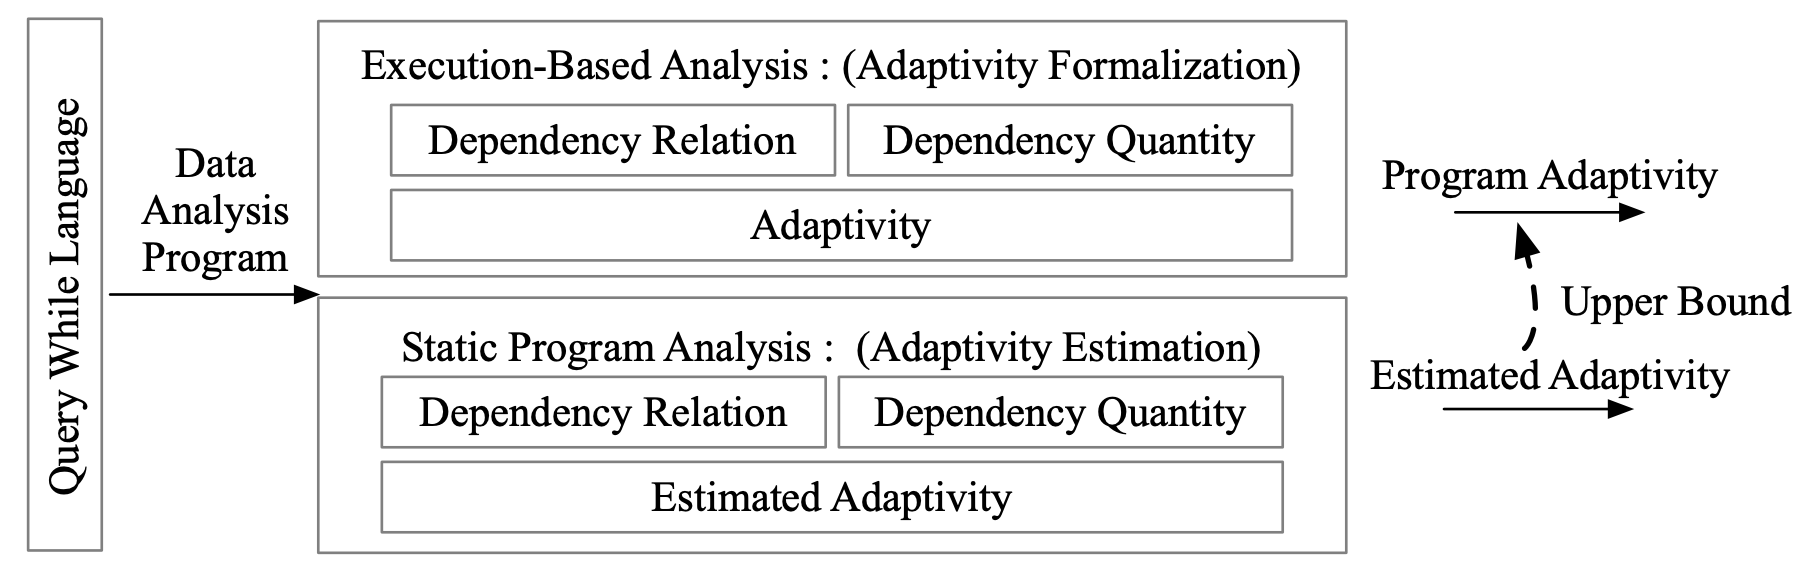
\includegraphics[width=1.0\textwidth]{figures/overview.png}
  \caption{Architecture of The Program Analysis Framework for Adaptivity Analysis}
   \label{fig:structure}
\end{figure}

\clearpage
\section{The {\tt Query While} Language}
\label{sec:adapt-language}
In this chapter, 
I formally introduce the language I will focus on for writing data analyses.  
This is a standard while language with some primitives for calling queries. 
After defining the syntax of the language and showing an example, 
I will define its trace-based operational semantics. 
This is the main technical ingredient I will use to define the program's adaptivity.
\section{Syntax of {\tt Query While} Language}
\label{sec:language-syntax}
The syntax is shown as follows,
\[
\begin{array}{llll}
\mbox{Arithmetic Operators} 
& \oplus_a & ::= & + ~|~ - ~|~ \times 
%
~|~ \div ~|~ \max ~|~ \min\\  
% \mbox{Unary Operators} 
% & \oplus_a & ::= & + ~|~ - ~|~ \times 
% %
% ~|~ \div \\  
\mbox{Boolean Operators} 
& \oplus_b & ::= & \lor ~|~ \land
\\
%
\mbox{Relational Operators} 
& \sim & ::= & < ~|~ \leq ~|~ == 
\\  
%
\mbox{Label} 
& l & \in & \mathbb{N} \cup \{\lin, \lex\} 
\\ 
%
\mbox{Arithmetic Expression} 
& \aexpr & ::= & 
n ~|~ {x} ~|~ \aexpr \oplus_a \aexpr  
% \\
% &  &  & 
 ~|~ \elog \aexpr  ~|~ \esign \aexpr
\\
%
\mbox{Boolean Expression} & \bexpr & ::= & 
%
\etrue ~|~ \efalse  ~|~ \neg \bexpr
 ~|~ \bexpr \oplus_b \bexpr
%
~|~ \aexpr \sim \aexpr 
\\
%
\mbox{Expression} & \expr & ::= & v ~|~ \aexpr ~|~ \bexpr ~|~ [\expr, \dots, \expr]
\\  
%
\mbox{Value} 
& v & ::= & { n ~|~ \etrue ~|~ \efalse ~|~ [] ~|~ [v, \dots, v]}  
\\
%
\highlight{\mbox{Query Expression}  }
& {\qexpr} & ::= 
& \highlight{ \qval ~|~ \aexpr ~|~ \qexpr \oplus_a \qexpr ~|~ \chi[\aexpr]}
\\
%
\highlight{\mbox{Query Value} }& \qval & ::= 
& \highlight{n ~|~ \chi[n] ~|~ \qval \oplus_a  \qval ~|~ n \oplus_a  \chi[n]
    ~|~ \chi[n] \oplus_a  n}
    \\
% &&& \text{\mg{I don’t think this is what I want. Isn’t $\chi[n+1]$ a query value?}}\\
% &&& \text{\mg{What about $\chi[i] + \chi[i] + \chi[i]$? They are not in the grammar}}
% \\
% &&& \text{\jl{ $\chi[i] + \chi[i] + \chi[i]$ and $\chi[n+1]$ are both expressions, they will be evaluated to a value 
% }}
% \\%
\mbox{Labeled Command} 
& {c} & ::= &   [\assign {{x}}{ {\expr}}]^{l} ~|~  \highlight{[\assign {{x} } {{\query(\qexpr)}}]^{l}}
~|~ {\ewhile [ \bexpr ]^{l} \edo {c} }
\\
&&&
~|~ {c};{c}  
~|~ \eif([\bexpr]{}^l , {c}, {c}) 
~|~ [\eskip]^l
\\ 
\mbox{Event} 
& \event & ::= & 
    ({x}, l, v, \bullet) ~|~ ({x}, l, v, \qval)  ~~~~~~~~~~~ \mbox{Assignment Event} \\
&&& ~|~(\bexpr, l, v, \bullet)   ~~~~~~~~~~~~~~~~~~~~~~~~~~~~~~~~~~ \mbox{Testing Event}
\\
\mbox{Trace} & \trace
& ::= & [] ~|~ \trace :: \event
\\
\end{array}
\]
% \[
% \begin{array}{llll}
% \mbox{Arithmetic Operators} 
% & \oplus_a & ::= & + ~|~ - ~|~ \times 
% %
% ~|~ \div ~|~ \max ~|~ \min\\  
% % ~|~ \div \\  
% \mbox{Boolean Operators} 
% & \oplus_b & ::= & \lor ~|~ \land
% \\
% %
% \mbox{Relational Operators} 
% & \sim & ::= & < ~|~ \leq ~|~ == 
% \\  
% %
% \mbox{Arithmetic Expression} 
% & \aexpr & ::= & 
% n ~|~ {x} ~|~ \aexpr \oplus_a \aexpr  
%  ~|~ \elog \aexpr  ~|~ \esign \aexpr
% \\
% %
% \mbox{Boolean Expression} & \bexpr & ::= & 
% %
% \etrue ~|~ \efalse  ~|~ \neg \bexpr
%  ~|~ \bexpr \oplus_b \bexpr
% %
% ~|~ \aexpr \sim \aexpr 
% \\
% %
% \mbox{Expression} & \expr & ::= & v ~|~ \aexpr ~|~ \bexpr ~|~ [\expr, \dots, \expr] ~|~ \highlight{\fname}
% \\  
% %
% \mbox{Value} 
% & v & ::= & { n ~|~ \etrue ~|~ \efalse ~|~ [] ~|~ [v, \dots, v]}  
% \\ 
% &&&
% \highlight
% {
% ~|~ (x_0, x_1, \ldots, x_n) := c
% }
% \\
% %
% \highlight{\mbox{Query Expression}} 
% & {\qexpr} & ::= 
% & \highlight{ \qval ~|~ \aexpr ~|~ \qexpr \oplus_a \qexpr ~|~ \chi[\aexpr]} 
% \\
% %
% \mbox{Query Value} & \qval & ::= 
% & \highlight{n ~|~ \chi[n] ~|~ \qval \oplus_a  \qval ~|~ n \oplus_a  \chi[n]
%     ~|~ \chi[n] \oplus_a  n}
% \\
% % \\%
% \mbox{Label} 
% & l & ::= & (n \in \mathbb{N} \cup \{\lin, \lex\}) ~|~ (l, n)
% \\ 
% %
% \mbox{Labeled Command} 
% & {c} & ::= &  
% \clabel{\assign{x}{\expr}}^l 
% ~|~ \clabel{\assign{x}{\query(\qexpr)}}^l
% ~|~  \clabel{\eskip}^l
% ~|~ \ewhile \clabel{\bexpr}^{l} \edo {c}
% ~|~ \eif(\clabel{\bexpr}^{l} , {c}, {c}) 
% \\ 
% &&&
% \highlight
% {
% ~|~ \clabel{\efun}^l: \fname (x_0, x_1, \ldots, x_n) := c
% ~|~ \clabel{\assign{x}{\ecall(x, e_1, \ldots, e_n)}}^l
% }
% ~|~ {c};{c}  
% \\ 
% % \\
% \mbox{Event} 
% & \event & ::= & 
%     ({x}, l, v, \bullet) ~|~ ({x}, l, v, \qval) ~|~ (\fname, l, v, \qval)  ~~~~~~~~~~~ \mbox{Assignment Event} \\
% &&& ~|~(\bexpr, l, v, \bullet)   ~~~~~~~~~~~~~~~~~~~~~~~~~~~~~~~~~~ \mbox{Testing Event}
% \\
% % &&& \text{\mg{I think it would be better to use quadruples for events, where the}}\\
% % &&& \text{\mg{first element is either a variable or a boolean expression and }}\\
% % &&& \text{\mg{the last is either a query value or some default value $\bullet$}}\\
% %
% % \mbox{Trace} & \trace
% % & ::= & \cdot | \trace \cdot \event | \trace \tracecat \trace 
% % \\
% %
% % \mbox{Trace} & \trace
% % & ::= & [] ~|~ \event:: \trace ~|~ \trace \tracecat \trace  \\
% \mbox{Trace} & \trace
% & ::= & [] ~|~ \trace :: \event\\
% % &&& \text{\mg{I don't understand why you need both :: and ++ as constructors.}}\\
% % &&& \text{\jl{Because append is to the left but we are adding element to the left in the OS}}\\
% % &&& \text{\jl{I was too sticky to the convention, it is a good idea to append to the left and just use $::$}}
% % %
% % \mbox{Event Signature} & \sig
% % & ::= & (x, l, n) | (x, l, n, \query) | (b, l, n)
% % \\
% % %
% \end{array}
% \]
For clarity, the following notations are used to represent the set of corresponding terms:
\[
\begin{array}{lll}
\mathcal{VAR} & : & \mbox{Set of Variables}  
\\ 
%
\mathcal{VAL} & : & \mbox{Set of Values} 
\\ 
%
\mathcal{QVAL} & : & \mbox{Set of Query Values} 
\\ 
%
\cdom & : & \mbox{Set of Commands} 
\\ 
%
\mathcal{LV} & : & \mbox{Set of Labeled Variables}
\\
%
\eventset  & : & \mbox{Set of Events}  
\\
%
\eventset^{\asn}  & : & \mbox{Set of Assignment Events}  
\\
%
\eventset^{\test}  & : & \mbox{Set of Testing Events}  
\\
%
\ldom  & : & \mbox{Set of Labels}  
\\
%%
\mathcal{VAL}  & : & \mbox{Set of Labeled Variables}  
\\
%%
\dbdom  & : & \mbox{{Set of Databases}} 
\\
%
{\mathcal{T}} & : & \mbox{Set of Traces}
\\
%
% \qdom = {[-1,1]} & : & \mbox{{Domain of Query Results}}\\
\qdom & : & \mbox{{Domain of Query Results}}\\
% &&\text{\mg{I don't think you need to hard code [-1,1] here}}\\
\end{array}
\]
\paragraph*{Standard Expression}
The expressions are either the standard one or the extended one.
A standard expression is
% can be 
either a standard arithmetic expression or a boolean expression, or a list of expressions.
An arithmetic expression can be a constant $n$ denoting integer, a variable $x$ from some countable set $\mathcal{VAR}$, binary operation $\oplus_a$ such as addition, product, subtraction, etc, over arithmetic expressions, and also log and sign operation. 
%
A boolean expression can be either {\tt true} or {\tt false}, basic boolean connectives such as logical negation, logical and and or denoted by $\oplus_b$, and basic comparison $sym$ between arithmetic expressions, e.g., $\leq,=,<,$ etc.
Additionally, I also introduce list in expression.
Our language supports primitives for queries, 
where a specific query is specified by a query expression $\qexpr$. 
A query expression contains the necessary information for a query request, for example, 
$\chi[\aexpr]$ represents the values at a certain index $\aexpr$ in a row $\chi$ of the database. 
Query expressions combine access to the database with other expressions, 
for example, $\chi[3] + 5$ represents a query which asks the value from the column 3 of each database raw $\chi$, adds 5 to each of these values, 
and then computes the average of these values.
\paragraph*{Query Expression}
The key extension is
%  language supports 
the primitive for queries, where a specific query is specified by a query expression $\qexpr$. 
A query expression contains the necessary information for a query request, 
for example, $\chi[\qexpr]$ represents the values at a certain index $\qexpr$ in a row $\chi$ of the database. 
When this expression is encapsulated by the symbol $\query$,
 $ \query(\chi[\qexpr]) $ computes the average value at certain index over each row of the database as follows,
 \[
  \query(\chi[\qexpr]) = \frac{1}{n}\sum\limits_{i = 0}^{n}\chi_i[\qexpr]
  \]
Query expressions combine access to the database with other expressions, 
for example, 
$\chi[3] + 5$ represents a query that asks the value from column 3 of each database raw $\chi$, 
adds 5 to each of these values, and then computes the average of these values as follows, where $n$ is 
data base $\chi$'s number of raw.
%
\[
  \query(\chi[3] + 5) = \frac{1}{n}\sum\limits_{i = 0}^{n}\chi_i[3] + 5
  \]

% the expression also includes the special variable $\chi$ representing a row of the database, and access to values at a certain index in $\chi$, as $\chi[\aexpr]$. Additionally, list over expressions is supported and $[]$ stands for the empty list. The access to elements in the list can be achieved through $x[\aexpr]$ when variable $x$ is referred to a list. The value $v$ now contains the natural number $n$, the boolean primitives $\etrue$ and $\efalse$, the special row $\chi$ and access to it $\chi[v]$, the empty list $[]$ and non-empty list $[v, \dots, v]$.
% 
% Another extension is the inter-procedure call and function definition.
% In the function define command $\clabel{\efun}^l: \fname (x_0, x_1, \ldots, x_n) := c$,
% the function body $c$ is assigned to the function of name $\fname$, $x_1, \ldots, x_n$ is the function
% arguments and the first element $x_0$ in the arguments is the return variable.
% We only support the first-order function definition and function call. 

% %
\paragraph*{Labeled Command}
 A labeled command $c$ is just a command with a label --- I assume that labels are unique, so that they can help to identify uniquely every subexpression. 
%  I have $\eskip$, assignment $\assign{x}{\expr}$, the composition of two commands $c;c$, an if statement $\eif(\bexpr, c, c)$, a while statement  $\ewhile \bexpr \edo {c} $.
 The main novelty of the syntax is the query request command $\assign{x}{\query(\qexpr)}$. 
 For instance, if a data analyst wants to ask a simple linear query which returns the first element of the row, 
 they can simply use the command $ \assign{x}{\query(\chi[1])}$ in their data analysis program.
%  \wq{Shall I distinguish command and labeled command, they are now both $c$. }
%  \jl{I'm not sure, I don't want to programmer to add the label when writing the program. The label is just added by us for analysis. but I'm worried it is too complicate if use two notations for command and labeled command }
%
% \[
% \begin{array}{llll}
% \mbox{Label} 
% & l & \in & \mathbb{N} \cup \{in, ex\} \\
% \mbox{Labeled Commands} 
% & {c} & ::= &   [\assign {{x}}{ {\expr}}]^{l} ~|~  [\assign {{x} } {{\query(\qexpr)}}]^{l}
% ~|~ {\ewhile [ \bexpr ]^{l} \edo {c} }
%  \\
%  &&&
% ~|~ {c};{c}  
% ~|~ \eif([\bexpr]{}^l , {c}, {c}) 
% ~|~ [\eskip]^l 
% \end{array}
% \]
\paragraph*{Labeled Variables}
The labeled variables and assigned variables are set of variables annotated by a label. 
We use  
%$\mathcal{LVAR} = \mathcal{VAR} \times \mathcal{L} $ 
$\mathcal{LV}$ represents the universe of all the labeled variables and 
$\avar_c \in \mathcal{P}(\mathcal{VAR} \times \mathbb{N}) \subset \mathcal{LV}$ and 
$\lvar_c \in \mathcal{P}(\mathcal{VAR} \times \mathcal{L}) \subseteq \mathcal{LV}$,
represents the the set of assigned variables and labeled variables for a labeled command $c$,
defined in Definition~\ref{def:lvar} and \ref{def:avar}.
%
% \\
$FV: \expr \to \mathcal{P}(\mathcal{VAR})$, computes the set of free variables in an expression. To be precise,
$FV(\aexpr)$, $FV(\bexpr)$ and $FV(\qexpr)$ represent the set of free variables in arithmetic
expression $\aexpr$, boolean expression $\bexpr$ and query expression $\qexpr$ respectively.
Labeled variables in $c$ is the set of assigned variables and all the free variables
showing up in $c$ with a default label $in$. 
The free variables
showing up in $c$, which aren't defined before be used, are actually the input variables of this program.
%
%
\begin{defn}[Assigned Variables (
% $\avar_{c} \subseteq \mathcal{VAR} \times \mathbb{N}$ or 
$\avar : \cdom \to \mathcal{P}(\mathcal{VAR} \times \mathbb{N})$)]
% labelled Variables 
% (
% % $\lvar_{c} \subseteq \mathcal{VAR} \times \mathbb{N}$ or 
% $\lvar : \cdom \to \mathcal{P}(\mathcal{VAR} \times \mathcal{L})$
\label{def:avar}
$$ \avar_{c} \triangleq
  \left\{
  \begin{array}{ll}
      \{{x}^l\}                   
      & {c} = [{\assign x e}]^{l} 
      \\
      \{{x}^l\}                   
      & {c} = [{\assign x \query(\qexpr)}]^{l} 
      \\
      \avar_{{c_1}} \cup \avar_{{c_2}}  
      & {c} = {c_1};{c_2}
      \\
      \avar_{{c}} \cup \avar_{{c_2}} 
      & {c} =\eif([\bexpr]^{l}, c_1, c_2) 
      \\
      \avar_{{c}'}
      & {c}   = \ewhile ([\bexpr]^{l}, {c}')
\end{array}
\right.
$$
\end{defn}
%
%
\begin{defn}[labelled Variables 
(
% $\lvar_{c} \subseteq \mathcal{VAR} \times \mathbb{N}$ or 
$\lvar : \cdom \to \mathcal{P}(\mathcal{LV})$]
\label{def:lvar}
$$
  \lvar_{c} \triangleq
  \left\{
  \begin{array}{ll}
      \{{x}^l\} \cup FV(\expr)^{in}                  
      & {c} = [{\assign x e}]^{l} 
      \\
      \{{x}^l\}   \cup FV(\qexpr)^{in}                
      & {c} = [{\assign x \query(\qexpr)}]^{l} 
      \\
      \lvar_{{c_1}} \cup \lvar_{{c_2}}  
      & {c} = {c_1};{c_2}
      \\
      \lvar_{{c}} \cup \lvar_{{c_2}} \cup FV(\bexpr)^{in}
      & {c} =\eif([\bexpr]^{l}, c_1, c_2) 
      \\
      \lvar_{{c}'} \cup FV(\bexpr)^{in}
      & {c}   = \ewhile ([\bexpr]^{l}, {c}')
\end{array}
\right.
$$
\end{defn}
%
%
%
% is a subset of the program's assigned variables, where every variable in this set is assigned by a query in the program.
% \mg{The set of query variables of a program is the set of variables set to the result of a query in the program.}\\
% In the same way, in order to 
\paragraph*{Query Variables}
Distinctively, a key definition for the extension of the query primitives 
is the set of query variables for a program $c$.
This definition is the key point to track the query requests in the Following full-spectrum adaptivity analysis.
% track the I also defined the set of query variables for a program $c$.
It is defined as the set of variables,
which are assigned by the result of a query request in the program formally in Definition~\ref{def:qvar}.
% \mg{In the next definition, why do you call it a vector? It seems that you define it as a set.}\\
% \jl{fixed}\\
%
% \begin{defn}[Query Variables ($\qvar_{c} \subseteq \mathcal{VAR} \times \mathbb{N}$)].
  % \\
\begin{defn}[Query Variables ($\qvar: \cdom \to \mathcal{P}(\mathcal{LV})$)] 
  \label{def:qvar}
Given a program $c$, its query variables 
% \mg{it seems you are missing the $_c$ subscript. Also, this is a minor point but I don't think it is a good idea to use a subscript, cannot you just use $\qvar(c)$.}
$\qvar(c)$ is the set of variables set to the result of a query in the program.
% \jl{fixed}
It is defined as follows:
{
$$
  % \qvar_{{c}} \triangleq
  \qvar(c) \triangleq
  \left\{
  \begin{array}{ll}
      % \{\}                  
      % & {c} = [{\assign x e}]^{(l, w)} 
      % \\
      % \{{x}^l\}                  
      % & {c} = [{\assign x \query(\qexpr)}]^{(l, w)} 
      % \\
      % \qvar_{{c_1}} \cup \qvar_{{c_2}}  
      % & {c} = {c_1};{c_2}
      % \\
      % \qvar_{{c_1}} \cup \qvar_{{c_2}} 
      % & {c} =\eif([\bexpr]^{l}, c_1, c_2) 
      % \\
      % \qvar_{{c}'}
      % & {c}   = \ewhile ([\bexpr]^{l}, {c}')
      \{\}                  
      & {c} = [{\assign x \expr}]^{l} 
      \\
      \{{x}^l\}                  
      & {c} = [{\assign x \query(\qexpr)}]^{l} 
      \\
      \qvar(c_1) \cup \qvar(c_2)  
      & {c} = {c_1};{c_2}
      \\
      \qvar(c_1) \cup \qvar(c_2) 
      & {c} =\eif([\bexpr]^{l}, c_1, c_2) 
      \\
      \qvar(c')
      & {c}   = \ewhile ([\bexpr]^{l}, {c}')
\end{array}
\right.
$$
}
\end{defn}
%
It is easy to see that a program $c$'s query variables is a subset of 
its labeled variables, $\qvar(c) \subseteq \lvar(c)$.
%
% \mg{In this definition as well as in others, I have the impression that you assume that the labelled variables are unique in the program. For example, it would not make sense to assign a query to the same labelled variable over and over. If this is the case, I need to make this very explicit in the paper.}
% \jl{TODO}
%
Every labeled variable in a program is unique, formally as follows with proof in Appendix~\ref{apdx:lemma_sec123}.
\begin{lem}[Uniqueness of the Labeled Variables]
  \label{lem:lvar_unique}
  For every program $c \in \cdom$ and every two labeled variables such that
  $x^i, y^j \in \lvar(c)$, then $x^i \neq y^j$.
  \[
    \forall c \in \cdom, x^i, y^j \in \mathcal{L} \sthat x^i, y^j \in \lvar(c)\implies x^i \neq y^j.
    \]
\end{lem}

\highlight{\paragraph*{Improvements through Examples}
It is expressive in two following aspects.
\begin{itemize}
  \item \textbf{Improvements from Standard While Language}
  \\
  It also extends the standard while language with query requests. 
  The general data analysis program with query requests on data  are supported in this {\tt Query While} language.
  The program can access the database through a special  interface $\chi$ encapsulated by the identifier $\query$ (for example the program below) in the new language.
  \[
    {\assign{x}{20}};
    \assign{y}{\query(\chi[2])};
    \ewhile (x < 100) \edo 
    \{
      \assign{x}{x + 1};
      \assign{y}{\query(\chi[x]*\chi[n])};
      \}\}
    \] 
%
    \item \textbf{Improvements from Previous Works}
  \\
This {\tt Query While} language is also more expressive than the language designed in previous works.
The previous language only supports the data analysis with constant number of loop iterations.
Comparing to it, in the new language design,
the general data analysis program with non-deterministic loop iterations
(for example the program below as shown in Section~\ref{sec:prework-language})
is supported.
\[
  {\assign{x}{20}};
  \assign{y}{40};
  \ewhile (x < y) \edo 
  \{
    \assign{x}{x + 1};
    \assign{y}{y - 2};
    \}\}
  \] 
Previous work does not support data analysis program with user inputs, which is supported in the new language as well.
\end{itemize}
}
\section{Trace-based Operational Semantics}
\label{sec:language-os}
The operational semantics is defined based on the event and trace, which are introduced firstly as follows.
% \\
\paragraph*{Event}
An event tracks useful information about each step of the evaluation, as a quadruple. Its first element is either 
an assigned variable (from an assignment command) or a boolean expression (from the guard of if or while command), follows by 
 the label associated with this event, the value evaluated either from the expression assigned to the variable,
or the boolean expression in the guard.
 The last element stores the query information, which is a query value whose default is $\bullet$. I declare event projection operator $\pi_i$ which projects the $i$th element from an event.
\[
\begin{array}{llll}
\mbox{Event} 
& \event & ::= & 
 ({x}, l, v, \bullet) ~|~ ({x}, l, v, \qval) ~~~~~~~~~~~ \mbox{Assignment Event} 
~|~(\bexpr, l, v, \bullet) 
~~~~
\mbox{Testing Event}
% \mbox{Trace} & \trace
% & ::= & [] ~|~ \trace :: \event
\end{array}
\]
% \input{event}
% To distinguish if a query's choice is affected by previous values, 
% % \jl{we need to be able to identify whether two queries are equivalent or not so that when we change the result of one query, another query is affected. For the equivalence of queries, } 
% we need to be able to identify whether two queries are equivalent or not, so that when we change the result of one query, whether or not another query is affected. 
% To define equivalence of queries,
% quite different from the equality between the evaluation results as the regular assignment results, 
% we are neither observing the syntactic equivalence between the two query expressions,
% nor two results return from the database. 
% Instead, we define the equivalence of query expression by quantifying over all values returned from the database on a certain form of query value, formally as follows.
% \begin{defn}[Equivalence of Query Expression]
% %
% \label{def:query_equal}
% % \mg{Two} \sout{2} 
% Two query expressions $\qexpr_1$, $\qexpr_2$ are equivalent, denoted as $\qexpr_1 =_{q} \qexpr_2$, if and only if
% % $$
% % \begin{array}{l} 
% % \exists \qval_1, \qval_2 \in \mathcal{QVAL} \st \forall \trace \in \mathcal{T} \st
% % (\config{\trace, \qexpr_1} \qarrow \qval_1 \land \config{\trace, \qexpr_2 } \qarrow \qval_2) 
% % \\
% % \quad \land (\forall D \in \dbdom, r \in D \st 
% % \exists v \in \mathcal{VAL} \st 
% % \config{\trace, \qval_1[r/\chi]} \aarrow v \land \config{\trace, \qval_2[r/\chi] } \aarrow v) 
% % \end{array}.
% % $$
% $$
% \begin{array}{l} 
% \forall \trace \in \mathcal{T} \st \exists \qval_1, \qval_2 \in \mathcal{QVAL} \st
% (\config{\trace, \qexpr_1} \qarrow \qval_1 \land \config{\trace, \qexpr_2 } \qarrow \qval_2) 
% \\
% \quad \land (\forall D \in \dbdom, r \in D \st 
% \exists v \in \mathcal{VAL} \st 
% \config{\trace, \qval_1[r/\chi]} \aarrow v \land \config{\trace, \qval_2[r/\chi] } \aarrow v) 
% \end{array}.
% $$
% % \mg{$$
% % \begin{array}{l} 
% % \forall \trace \in \mathcal{T} \st \exists \qval_1, \qval_2 \in \mathcal{QVAL} \st
% % (\config{\trace, \qexpr_1} \qarrow \qval_1 \land \config{\trace, \qexpr_2 } \qarrow \qval_2) 
% % \\
% % \quad \land (\forall D \in \dbdom, r \in D \st 
% % \exists v \in \mathcal{VAL} \st 
% % \config{\trace, \qval_1[r/\chi]} \aarrow v \land \config{\trace, \qval_2[r/\chi] } \aarrow v) 
% % \end{array}.
% % $$
% % }
% %
% where $r \in D$ is a record in the database domain $D$. 
% I denote by $\qexpr_1 \neq_{q} \qexpr_2$ the negation of the equivalence relation.
% % \\ 
% % where $r \in D$ is a record in the database domain $D$,
% % \mg{is $FV(\qexpr)$ being defined here? If yes, I suggest putting it in a different place, rather than in the middle of another definition.} 
% % $FV(\qexpr)$ is the set of free variables in the query expression $\qexpr$.
% % \sout{$\qexpr_1 \neq_{q}^{\trace} \qexpr_2$ is defined vice versa.}
% % \mg{As usual, we will denote by $\qexpr_1 \neq_{q}^{\trace} \qexpr_2$ the negation of the equivalence.}
% %
% \end{defn}
%
% \mg{In the next definition you don’t need the subscript e, it is clear that it is an equivalence of events by the fact that the elements on the two sides of = are events. That is also true for query expressions. Also, I am confused by this definition. What happens for two query events?}
% \\
% \jl{The last component of the event is equal based on Query equivalence, $\pi_{4}(\event_1) =_q \pi_{4}(\event_2)$.
% In the previous version, the query expression is in the third component and I defined $v \neq \qexpr$ for all $v$ that isn't a query value.}
% \begin{defn}[Event Equivalence $\eventeq$]
% Two events $\event_1, \event_2 \in \eventset$ \mg{are equivalent, \sout{is in \emph{Equivalence} relation,}} denoted as $\event_1 \eventeq \event_2$ if and only if:
% \[
% \pi_1(\event_1) = \pi_1(\event_2) 
% \land 
% \pi_2(\event_1) = \pi_2(\event_2) 
% \land
% \pi_{3}(\event_1) = \pi_{3}(\event_2)
% \land 
% \pi_{4}(\event_1) =_q \pi_{4}(\event_2)
% \]
% %
% % \sout{The $\event_1 \eventneq \event_2$ is defined as vice versa.}
% % \mg{As usual, we will denote by $\event_1 \eventneq \event_2$ the negation of the equivalence.}
% \end{defn}
% \wq{Now we can compare two events by defining the event equivalence and difference relation.}
% Now we can compare two events by defining the event equivalence and difference relation based on the query equivalence.
% \begin{defn}[Event Equivalence]
% \label{def:event_eq}
% Two events $\event_1, \event_2 \in \eventset$ are equivalent, 
% % denoted as $\event_1 \eventeq \event_2$ 
% denoted as $\event_1 = \event_2$ 
% if and only if:
% \[
% \pi_1(\event_1) = \pi_1(\event_2) 
% \land 
% \pi_2(\event_1) = \pi_2(\event_2) 
% \land
% \pi_{3}(\event_1) = \pi_{3}(\event_2)
% \land 
% \pi_{4}(\event_1) =_q \pi_{4}(\event_2)
% \]
% %
% As usual, we will denote by $\event_1 \neq \event_2$ the negation of the equivalence.
% % As usual, we will denote by $\event_1 \eventneq \event_2$ the negation of the equivalence.
% % When it is clear from the context, we omit the subscript $\kw{e}$ and use 
% % $\event_1 = \event_2$ (and $\event_1 \neq \event_2$) for event equivalent
% \end{defn}
% %
% %
% % \begin{defn}[Signature Equivalence of Events $\sigeq$]
% % Two events $\event_1, \event_2 \in \eventset$ is in \emph{signature equivalence} relation, denoted as $\event_1 \sigeq \event_2$ if and only if:
% % \[
% % \forall i \in \{1, 2, 3\} \st \pi_{\sig}(\event_1) = \pi_{\sig}(\event_2) 
% % \]
% % The $\event_1 \signeq \event_2$ is defined as vice versa.
% % \end{defn}
% %
% % \begin{defn}[Events Different up to Value ($\diff$)]
% % Two events $\event_1, \event_2 \in \eventset$ \mg{are \sout{is}} \emph{Different up to Value}, 
% % denoted as $\diff(\event_1, \event_2)$ if and only if:
% % \[
% % \pi_1(\event_1) = \pi_1(\event_2) 
% % \land 
% % \pi_2(\event_1) = \pi_2(\event_2) 
% % \land 
% % \pi_3(\event_1) \neq_q \pi_3(\event_2)
% % \]
% % \end{defn}
% \begin{defn}[Events Different up to Value ($\diff$)]
% Two events $\event_1, \event_2 \in \eventset$ are \emph{Different up to Value}, 
% denoted as $\diff(\event_1, \event_2)$ if and only if:
% \[
% \begin{array}{l}
% \pi_1(\event_1) = \pi_1(\event_2) 
% \land 
% \pi_2(\event_1) = \pi_2(\event_2) \\
% \land 
% \big(
% (\pi_3(\event_1) \neq \pi_3(\event_2)
% \land 
% \pi_{4}(\event_1) = \pi_{4}(\event_2) = \bullet )
% % \qquad \qquad 
% \lor 
% (\pi_4(\event_1) \neq \bullet
% \land 
% \pi_4(\event_2) \neq \bullet
% \land 
% \pi_{4}(\event_1) \neq_q \pi_{4}(\event_2)) 
% \big)
% \end{array}
% \]
% \end{defn}
% %
% %
\paragraph*{Trace}
A trace $\trace \in \mathcal{T} $ is a list of events, 
collecting the events generated along the program execution. $\mathcal{T} $ represents the set of traces. There are some useful operators: the trace concatenation operator $\tracecat: \mathcal{T} \to \mathcal{T} \to \mathcal{T}$, combines two traces.
The belongs to operator $\in : \eventset \to \mathcal{T} \to \{\etrue, \efalse \} $ and its opposite $\not\in$
express whether or not an event belongs to a trace.
Another operator $\llabel : \mathcal{T} \to \mathcal{VAR} \to \{\mathbb{N}\}\cup \{\bot\}$,
takes a trace and a variable as input and returns the label of the latest assignment event which assigns value to that variable. 
% I also have the operator $\tlabel : \mathcal{T} \to \ldom$, which gives the set of labels in every event belonging to a trace. 
% The full definitions of these above operators can be found in the appendix.
% \[
% \begin{array}{llll}
% \mbox{Trace} & \trace
% & ::= & [] ~|~ \trace :: \event
% \end{array}
% \]
%
A trace can be regarded as the program history, which records queries asked by the analyst during the execution of the program. I collect the trace with a trace-based operational semantics based on transitions of the form $ \config{c, \trace} \to \config{c', \trace'} $. It states that a configuration $\config{c, \trace}$, which consists of a command $c$ to be evaluated and a starting trace $\trace$, evaluates to another configuration with the trace updated along with the evaluation of the command $c$ to the normal form of the command $\eskip$.
% \jl{I introduce some operations here: the trace concatenation $\tracecat: \mathcal{T} \to \mathcal{T} \to \mathcal{T}$, which combines two traces; they belong to operator $\in$ so that an event $\event \in \eventset$ belongs to a trace $\trace$ is notated by $\event \in \trace$. 
% As usual, we denote by $\event \notin \trace$ that the event $\event$ doesn't belong to the trace $\trace$. 
% Another operator $\llabel : \mathcal{T} \to \mathcal{VAR} \to \{\mathbb{N}\}\cup \{\bot\}$,
% takes a trace and a variable and returns the label of the latest assignment event which assigns value to that variable. I also have the operator $\tlabel : \mathcal{T} \to \mathcal{P}{(\mathbb{N})}$, which gives the set of labels in every event belonging to a trace. The full definitions of these above operators can be found in the appendix.
% }
% \wq{It seems trace concatenation and event belonging to a trace do not deserve so much space here:-)}
%\jl{I agree}

% \\
% I also introduce a counting operator $\vcounter : \mathcal{T} \to \mathbb{N} \to \mathbb{N}$, 
% % \wq{which counts the occurrence of a variable in the trace,} 
% which counts the occurrence of a labeled variable in the trace,
% whose behavior is defined as follows,
% % \[
% % \begin{array}{lll}
% % \vcounter(\trace :: (x, l, v, \bullet) ) l \triangleq \vcounter(\trace) l + 1
% % &
% % \vcounter(\trace ::(b, l, v, \bullet) ) l \triangleq \vcounter(\trace) l + 1
% % &
% % \vcounter(\trace :: (x, l, v, \qval) ) l \triangleq \vcounter(\trace) l + 1
% % \\
% % \vcounter(\trace :: (x, l', v, \bullet) ) l \triangleq \vcounter(\trace ) l, l' \neq l
% % &
% % \vcounter(\trace :: (b, l', v, \bullet) ) l \triangleq \vcounter(\trace ) l, l' \neq l
% % &
% % \vcounter(\trace :: (x, l', v, \qval)) l \triangleq \vcounter(\trace ) l, l' \neq l
% % \\
% % \vcounter({[]}) l \triangleq 0
% % &&
% % \end{array}
% % \]
% \[
% \begin{array}{lll}
% \vcounter(\trace :: (x, l, v, \bullet), l ) \triangleq \vcounter(\trace, l) + 1
% &
% \vcounter(\trace ::(b, l, v, \bullet), l) \triangleq \vcounter(\trace, l) + 1
% &
% \vcounter(\trace :: (x, l, v, \qval), l) \triangleq \vcounter(\trace, l) + 1
% \\
% \vcounter(\trace :: (x, l', v, \bullet), l) \triangleq \vcounter(\trace, l), l' \neq l
% &
% \vcounter(\trace :: (b, l', v, \bullet), l) \triangleq \vcounter(\trace, l), l' \neq l
% &
% \vcounter(\trace :: (x, l', v, \qval), l) \triangleq \vcounter(\trace, l), l' \neq l
% \\
% \vcounter({[]}, l) \triangleq 0
% &&
% \end{array}
% \]
% \input{trace}
%%% trace, queries
% A memory is standard, a map from variables to values. Queries can be uniquely annotated as $\mathcal{AQ}$, and the annotation $(l,w)$ considers the location of the query by line number $l$ and which iteration the query is at when it appears in a loop statement, specified by $w$. A trace $t$ is a list of annotated queries accumulated along the execution of the program. 



\paragraph*{Environment}
The function $\env : {\mathcal{T}} \to \mathcal{VAR} \to \mathcal{VAL} \cup \{\bot\}$, which maps a trace and a variable to the latest value assigned to this variable on the trace is defined as follows.
% \wq{Question: Seem $\env$ is a function that looks up in the input trace and returns you the latest value of the variable. I have a question, in the two-round example, I see $env(\tau)(k)$ while $k$ is not defined(it is input), so in our two-round example in Overview, the value is stored in the second event is $\bot$? Also, another important, $\env$ relies on the input trace, so it will not appear in the trace, or config, is it precise?}
% \jl{yes, it is precise. 
% I have initial trace and everything belonging is defined over all possible initial traces.
%in the two-round example, there is an initial trace where the value of k is defined there. It is worth explaining this here.
% }
\[
\begin{array}{lll}
\env(\trace \traceadd (x, l, v, \bullet)) x \triangleq v
&
\env(\trace \traceadd (y, l, v, \bullet)) x \triangleq \env(\trace) x, y \neq x
&
\env(\trace \traceadd (b, l, v, \bullet)) x \triangleq \env(\trace) x
\\
\env(\trace \traceadd (x, l, v, \qval)) x \triangleq v
&
\env(\trace \traceadd (y, l, v, \qval)) x \triangleq \env(\trace) x, y \neq x
&
\env({[]} ) x \triangleq \bot
\end{array}
\]
 %% trace

%
% figure, evaluation rules.
% {\footnotesize
% \begin{figure}
% \begin{mathpar}
% \boxed{ \config{m, c, t,w} \xrightarrow{} \config{m', c', t', w'} \; }
% \and
% %
% {\inferrule
% {
% \valr_N > 0
% }
% {
% \config{m, \eloop ~ [\valr_N]^{l} ~ \edo ~ c , t, w }
% \xrightarrow{} \config{m, c ; \eloop ~ [(\valr_N-1)]^{l} ~ \edo ~ c , t, (w + l) }
% }
% ~\textbf{low-loop}
% }
% %
% \and
% %
% \inferrule
% {
% }
% {
% \config{m, [\eskip]^{l} ; c_2, t,w} \xrightarrow{} \config{m, c_2, t,w}
% }
% ~\textbf{low-seq2}
% %
% \quad
% %
% {
% \inferrule
% {
% \valr_N = 0
% }
% {
% \config{m, \eloop ~ [\valr_N]^{l} ~ \edo ~ c , t, w }
% \xrightarrow{} \config{m, [\eskip]^{l} , t, (w \setminus l) }
% }
% ~\textbf{low-loop-exit}
% }
% \and
% %
% \inferrule
% {
% }
% {
% \config{m, \eif([\efalse]^{l}, c_1, c_2), t,w} 
% \xrightarrow{} \config{m, c_2, t,w}
% }
% ~\textbf{low-if-f}
% %
% ~~
% % { Memory \times Com \times Trace \times WhileMap \Rightarrow^{} Memory \times Com \times Trace \times WhileMap}
% \inferrule
% {
% \config{m,\expr} \to \expr'
% }
% {
% \config{m, [\assign{x}{q(\expr)}]^l, t, w} \xrightarrow{} \config{m, [\assign{x}{q(\expr')}]^l, t, w}
% }
% ~\textbf{low-query-e}
% %
% \and
% %
% %
% \inferrule
% {
% \config{m, c_1, t,w} \xrightarrow{} \config{m', c_1', t',w'}
% }
% {
% \config{m, c_1; c_2, t,w} \xrightarrow{} \config{m', c_1'; c_2, t',w'}
% }
% ~\textbf{low-seq1}
% ~~
% \inferrule
% {
% q(v) = v_q
% }
% {
% \config{m, [\assign{x}{q(v)}]^l, t, w} \xrightarrow{} \config{m[ v_q/ x], \eskip, t \mathrel{++} [q(v)^{(l,w )}],w }
% }
% ~\textbf{low-query-v}
% %
% % \inferrule
% % {
% % }
% % {
% % \config{m, [\assign x v]^{l}, t,w} \xrightarrow{} \config{m[v/x], [\eskip]^{l}, t,w}
% % }
% % ~\textbf{low-assn}
% %
% %
% %
% \and
% %
% \inferrule
% {
% \config{ m, \bexpr} \barrow \bexpr'
% }
% {
% \config{m, \eif([\bexpr]^{l}, c_1, c_2), t,w} 
% \xrightarrow{} \config{m, \eif([\bexpr']^{l}, c_1, c_2), t,w}
% }
% ~\textbf{low-if}
% %
% ~~~~
% %
% \inferrule
% {
% }
% {
% \config{m, \eif([\etrue]^{l}, c_1, c_2),t,w} 
% \xrightarrow{} \config{m, c_1, t,w}
% }
% ~\textbf{low-if-t}
% %
% % %
% %
% \end{mathpar}
% \vspace{-0.3cm}
% \caption{Trace-based operational semantics}
% \label{fig:evaluation}
% \vspace{-0.5cm}
% \end{figure}
% }
%
% explanation of rules

%
\begin{figure}
 \begin{mathpar}
 \boxed{
 \mbox{Command $\times$ Trace}
 \xrightarrow{}
 \mbox{Command $\times$ Trace}
 }
 \and
 \boxed{\config{{c, \trace}}
 \xrightarrow{} 
 \config{{c', \trace'}}
 }
 \\
 % \inferrule
 % {
 % \empty
 % }
 % {
 % \config{\clabel{\eskip}^l, \trace } 
 % \xrightarrow{} 
 % \config{\clabel{\eskip}^l, \trace}
 % }
 % ~\textbf{skip}
 %
 % \and
 %
 \inferrule
 {
 \config{\trace, \expr} \earrow v 
 \and
 \event = ({x}, l, v, \bullet)
 }
 {
 \config{[\assign{{x}}{\expr}]^{l}, \trace } 
 \xrightarrow{} 
 \config{\clabel{\eskip}^l, \trace \traceadd \event}
 }
 ~\textbf{assn}
 %
 \and
 %
 \highlight{
 \inferrule
 {
\config{ \trace, \qexpr} \qarrow \qval
 \and 
 \query(\qval) = v
 \and 
 \event = ({x}, l, v, \qval)
 }
 {
 \config{{[\assign{x}{\query(\qexpr)}]^l, \trace}}
 \xrightarrow{} 
 \config{{\clabel{\eskip}^l, \trace \traceadd \event} }
 }
 ~\textbf{query}
 }
 %
 \and
 %
 \inferrule
 {
\config{ \trace, b} \barrow \etrue
 \and 
 \event = (b, l, \etrue, \bullet)
 }
 {
 \config{{\ewhile [b]^{l} \edo c, \trace}}
 \xrightarrow{} 
 \config{{
 c; \ewhile [b]^{l} \edo c),
 \trace \traceadd \event}}
 }
 ~\textbf{while-t}
 %
 %
 \quad
 %
 \inferrule
 {
 \config{\trace, b} \barrow \efalse
 \and 
 \event = (b, l, \efalse, \bullet)
 }
 {
 \config{{\ewhile [b]^{l}, \edo c, \trace}}
 \xrightarrow{} 
 \config{{
 \clabel{\eskip}^l,
 \trace \traceadd \event}}
 }
 ~\textbf{while-f}
 %
 %
 \and
 %
 %
 \inferrule
 {
 \config{{c_1, \trace}}
 \xrightarrow{}
 \config{{\clabel{\eskip}^l, \trace'}}
 \and 
 \config{{\clabel{\eskip}^l; c_2, \trace'}} \xrightarrow{} \config{{ \clabel{\eskip}^l, \trace''}}
 }
 {
 \config{{c_1; c_2, \trace}} 
 \xrightarrow{} 
 \config{{\clabel{\eskip}^l, \trace''}}
 }
 ~\textbf{seq}
 %
 % \and
 % %
 % \inferrule
 % {
 % \config{{c_2, \trace}}
 % \xrightarrow{}
 % \config{{c_2', \trace'}}
 % }
 % {
 % \config{{\clabel{\eskip}^l; c_2, \trace}} \xrightarrow{} \config{{ c_2', \trace'}}
 % }
 % ~\textbf{seq2}
 %
 \quad
 %
 %
 \inferrule
 {
 \trace, b \barrow \etrue
 \and 
 \event = (b, l, \etrue, \bullet)
 }
 {
 \config{{
 \eif([b]^{l}, c_1, c_2), 
 \trace}}
 \xrightarrow{} 
 \config{{c_1, \trace \traceadd \event}}
 }
 ~\textbf{if-t}
 %
 % \and
 % %
 % \inferrule
 % {
 % \trace, b \barrow \efalse
 % \and 
 % \event = (b, l, \efalse, \bullet)
 % }
 % {
 % \config{{\eif([b]^{l}, c_1, c_2), \trace}}
 % \xrightarrow{} 
 % \config{{c_2, \trace \traceadd \event}}
 % }
 % ~\textbf{if-f}
 \end{mathpar}
 % \end{subfigure}
 \vspace{-0.5cm}
 \caption{Trace-based Operational Semantics for Language.}
 \label{fig:os}
 \end{figure}
 %

% {The big step trace-based operational semantics has the form of $ \config{c, \trace} \xrightarrow{} { \config{c', \trace'}}$. It reads that the configuration $(c, \trace)$ with labeled command $c$ and trace $\trace$, will be evaluated to another configuration, in which $c$ is evaluated to $c'$ and the trace is updated during the evaluation, to $\trace'$. 
% }
% The step trace-based operational semantics has the form of $ \config{c, \trace} \xrightarrow{} { \config{c', \trace'}}$. 
% It reads the configuration $\config{c, \trace}$ consisting of a labeled command $c$ and a pre-trace $\trace$, 
% and evaluates it to another configuration, 
% in which $c$ is evaluated to $c'$ and trace $\trace$ is updated to $\trace'$. 
% is updated during the evaluation,
\paragraph*{Operational Semantics}
I give a selection of rules of the trace-based operational semantics in Figure~\ref{fig:os}. 

% \todo{Make sure the operational semantics is a big step and correct assn rules.}
% \jl{
The rule $\textbf{assn}$ evaluates a standard assignment $\assign{x}{\expr}$, the expression $\expr$ is first evaluated by our expression evaluation $\config{\trace, \expr} \earrow v $, presented below. And the result $v$ of evaluating $\expr$ is used to construct a new event $\event = (x, l, v,\bullet)$ and attach it to the previous trace. 
\begin{mathpar}
% \boxed{ \config{\trace, \expr} \earrow v \, : \, \mbox{Trace $\times$ Expression $\Rightarrow$ Value} }
% \\
\inferrule{ 
 \config{\trace, \aexpr} \aarrow v
}{
 \config{\trace, \aexpr} 
 \earrow v
}
\and
\inferrule{ 
 \config{\trace, \bexpr} \barrow v
}{
 \config{\trace, \bexpr} 
 \earrow v
}
\and
\inferrule{ 
 \config{\trace, \expr_1} \earrow v_1
 \cdots
 \config{\trace, \expr_n} \earrow v_n
}{
 \config{\trace, [\expr_1, \cdots, \expr_n]} 
 \earrow [v_1, \cdots, v_n]
}
\and
\inferrule{ 
 \empty
}{
 \config{\trace, v} 
 \earrow v
}
\end{mathpar}
The expression evaluation rules also rely on the evaluation of arithmetic expressions $\config{\trace,\aexpr} \aarrow v $ and boolean expressions $\config{\trace, \bexpr} \barrow v $. The full rules can be found in the appendix.
% \begin{mathpar}
% \boxed{ \config{\trace,\aexpr} \aarrow v \, : \, \mbox{Trace $\times$ Arithmetic Expr $\Rightarrow$ Arithmetic Value} }
% % \text{\mg{Missing. Without these rules, it is difficult to understand why we need a trace to evaluate expressions.}}
% \\
% \inferrule{ 
% \empty
% }{
% \config{\trace, n} 
% \aarrow n
% }
% \and
% \inferrule{ 
% \env(\trace) x = v
% }{
% \config{\trace, x} 
% \aarrow v
% }
% \and
% \inferrule{ 
% \config{\trace, \aexpr_1} \aarrow v_1
% \and 
% \config{\trace, \aexpr_2} \aarrow v_2
% \and 
% v_1 \oplus_a v_2 = v
% }{
% \config{\trace, \aexpr_1 \oplus_a \aexpr_2} 
% \aarrow v
% }
% % \and
% % \inferrule{ 
% % \config{\trace, \aexpr} \aarrow v'
% % \and 
% % \elog v' = v
% % }{
% % \config{\trace, \elog \aexpr} 
% % \aarrow v
% % }
% % \and
% % \inferrule{ 
% % \config{\trace, \aexpr} \aarrow v'
% % \and 
% % \esign v' = v
% % }{
% % \config{\trace, \esign \aexpr} 
% % \aarrow v
% % }
% \\
% \boxed{ \config{\trace, \bexpr} \barrow v \, : \, \mbox{Trace $\times$ Boolean Expr $\Rightarrow$ Boolean Value} }
% % \text{\mg{Missing. Without these rules, it is difficult to understand why we need a trace to evaluate expressions.}}
% \\
% % \inferrule{ 
% % \empty
% % }{
% % \config{\trace, \efalse} 
% % \barrow \efalse
% % }
% % \and 
% % \inferrule{ 
% % \empty
% % }{
% % \config{\trace, \etrue} 
% % \barrow \etrue
% % }
% % \and 
% \inferrule{ 
% \config{\trace, \bexpr} \barrow v'
% \\ 
% \neg v' = v
% }{
% \config{\trace, \neg \bexpr} 
% \barrow v
% }
% \and 
% \inferrule{ 
% \config{\trace, \bexpr_1} \barrow v_1
% \\ 
% \config{\trace, \bexpr_2} \barrow v_2
% \\ 
% v_1 \oplus_b v_2 = v
% }{
% \config{\trace, \bexpr_1 \oplus_b \bexpr_2} 
% \barrow v
% }
% \and 
% \inferrule{ 
% \config{\trace, \aexpr_1} \aarrow v_1
% \\ 
% \config{\trace, \aexpr_2} \aarrow v_2
% \\ 
% v_1 \sim v_2 = v
% }{
% \config{\trace, \aexpr_1 \sim \aexpr_2} 
% \barrow v
% }
% \end{mathpar}
% % }


Distinguished from the standard assignment evaluation, 
the rule $\textbf{query}$ 
evaluates a query requesting command $\clabel{\assign{x}{\query(\qexpr)}}^l$ in two steps.
The query expression $\qexpr$ is first evaluated into a query value $\qval$ by following the rules below.
Then, by sending this query request $\query(\qval)$ to a hidden mechanism, this query is evaluated to a result value returned from it, $v = \query(\qval)$.
% by sending this query request $\query(\qval)$ to it.
Also, the generated event stores both the query value $\alpha$ here, and the result value of the query request.

\begin{mathpar}
% \boxed{ \config{\trace, \qexpr} \qarrow \qval \, : \, \mbox{Trace $\times$ Query Expr $\Rightarrow$ Query Value} }
% \\
\inferrule{ 
 \config{\trace, \aexpr} \aarrow n
}{
 \config{\trace, \aexpr} 
 \qarrow n
}
\and
\inferrule{ 
 \config{\trace, \qexpr_1} \qarrow \qval_1
 \and
 \config{\trace, \qexpr_2} \qarrow \qval_2
}{
 \config{\trace, \qexpr_1 \oplus_a \qexpr_2} 
 \qarrow \qval_1 \oplus_a \qval_2
}
\and
\inferrule{ 
 \config{\trace, \aexpr} \aarrow n
}{
 \config{\trace, \chi[\aexpr]} \qarrow \chi[n]
}
\and
\inferrule{ 
 \empty
}{
 \config{\trace, \qval} 
 \qarrow \qval
}
 \end{mathpar}
% }
% \wq{The rules for if hand while both have two versions, when the guard evaluates to true and false, respectively. In these rules, the evaluation of the guard also generates a testing event and our trace is updated as well. }
The rules for if and while both have two versions 
when the boolean expressions in the guards are evaluated to true and false, respectively. 
In these rules, the evaluation of the guard generates a testing event and the trace is updated as well by appending this event.
% The rule $\textbf{query}$ evaluates the argument of a query request to a normal form and obtains the answer $v_q$ of the query $\query(v)$ from the mechanism. 
% Then the trace is expanded by appending the query expression $\query(v)$ with the current annotation $(l,w)$. 

% The rule for assignment is standard and the trace remains unchanged. The sequence rule keeps tracking the modification of the trace, and the evaluation rule for if conditional 

% \jl{If we observe the operational semantics rules, we can find that no rule will shrink the trace.} 
% If we observe the operational semantics rules, we can find that no rule will shrink the trace. It is proved in the appendix.
% So we have the Lemma~\ref{lem:tracenondec}, specifically, the trace has the property that its length never decreases during the program execution.

% \begin{lem}
% [Trace Non-Decreasing]
% \label{lem:tracenondec}
% For every program $c \in \cdom$ and traces $\trace, \trace' \in \mathcal{T}$, if 
% $\config{c, \trace} \rightarrow^{*} \config{\eskip, \trace'}$,
% then there exists a trace $\trace'' \in \mathcal{T}$ with $\trace \tracecat \trace'' = \trace'$
% %
% $$
% \forall \trace, \trace' \in \mathcal{T}, c \st
% \config{c, \trace} \rightarrow^{*} \config{\eskip, \trace'} 
% \implies \exists \trace'' \in \mathcal{T} \st \trace \tracecat \trace'' = \trace'
% $$
% \end{lem}
% %
% % \mg{This corollary needs some explanation. In particular, we should stress that $\event$ and $\event'$ may differ in the query value.}
% % Since the equivalence over two events is defined over the query value equivalence, 
% % when there is an event 
% % belonging to a trace, 
% % it is possible that the event showing up in this trace has a different form of query value, but they are equivalent by Definition~\ref{def:query_equal}.
% Since the equivalence over two events is defined over the query value equivalence, 
% when there is an event belonging to a trace, 
% if this event is a query assignment event, 
% it is possible that 
% the event showing up in this trace has a different form of query value, 
% but they are equivalent by Definition~\ref{def:query_equal}.
% So we have the following Corollary~\ref{coro:aqintrace} with proof in Appendix.
% % ~\ref{apdx:lemma_sec123}.
% % \todo{we should stress that $\event$ and $\event'$ may differ in the query value.}
% \begin{coro}
% \label{coro:aqintrace}
% For every event and a trace $\trace \in \mathcal{T}$,
% if $\event \in \trace$, 
% then there exist another event $\event' \in \eventset$ and traces $\trace_1, \trace_2 \in \mathcal{T}$
% such that $\trace_1 \tracecat [\event'] \tracecat \trace_2 = \trace $
% with 
% $\event$ and $\event'$ equivalent but may differ in their query value.
% \[
% \forall \event \in \eventset, \trace \in \mathcal{T} \st
% \event \in \trace \implies \exists \trace_1, \trace_2 \in \mathcal{T}, 
% \event' \in \eventset \st (\event = \event') \land \trace_1 \tracecat [\event'] \tracecat \trace_2 = \trace 
% \]
% \end{coro}




\clearpage
\section{The Adaptivity Formalization}
\label{sec:adapt-exe}
% In this section, I present my 
% execution-based adaptivity analysis as the first part of the full-spectrum adaptivity analysis as in Figure~\ref{fig:structure}. 
In this section, 
I formally present a new execution-based program adaptivity analysis based on the language and the trace-based operational semantics introduced above.
As in Figure~\ref{fig:structure}, this is the second major part of this adaptivity analysis framework
built on the language design. 
It is more advanced than previous works
in both the accuracy and efficiency aspects.
This analysis formalizes the intuitive \emph{adaptivity} through three steps.
In Section~\ref{sec:dynamic-datadep}, I first give the new data dependency definition.
Then Section~\ref{sec:dynamic-reachability} presents the dependency quantity analysis for the dependency relation.
The  Section~\ref{sec:dynamic-adapt} gives the formal \emph{adaptivity} definition.
% ,~\ref{sec:dynamic-reachability}
% % I  an execution based program analysis in this section.
% and~\ref{sec:dynamic-adapt}.
Through an example in Section~\ref{sec:dynamic-examples}, I show that the formalized
% can give the 
adaptivity matches the program's intuitive \emph{adaptivity} more precisely and efficiently than previous works.

\paragraph*{Execution-Based Adaptivity Analysis Outline}
% To formalize this intuition as a quantitative program property, I develop an
This improved execution-based analysis is developed
% I first consider all the possible evaluations of a program --- I do this by 
% I use a trace semantics recording the execution history of programs on some given input --- and I create a dependency graph, where the dependency between different variables (query is also assigned to a variable) is explicit and track which variable is associated with a query request. 
% I then enrich this graph with weights describing the maximal number of times each variable is evaluated in a program evaluation starting with an initial state. The adaptivity is then defined as the length of the walk visiting most query-related variables on this graph. 
% Through two aspects: the execution-based analysis and static-based program analysis.
% In the execution-based analysis, I will formalize the intuitive notion of \emph{adaptivity} as a quantitative 
% property of programs. This analysis is developed 
 in three steps as follows,
 \begin{enumerate}
 \item The first step on \emph{dependency relation} analysis is presented in 
 Section~\ref{sec:dynamic-datadep}.
 In this step, I define the variable \emph{may-dependency} relation based on the trace semantics in Section~\ref{sec:language-os}.
%   to analyze the \emph{dependency relation} between every query, 
%  through the methodology of semantic data dependency analysis.
%  %
%  Specifically through a trace semantics recording the execution history of programs on given input,
%  % --- and I create a dependency graph, 
%  the dependency between different variables (query is also assigned to a variable) is explicitly tracked and 
%  analyzed.
%   and 
%   which variable is associated with a query request. 
% I then enrich this graph with weights describing the maximal number of times each variable is evaluated in a program evaluation starting with an initial state. The adaptivity is then defined as the length of the walk visiting most query-related variables on this graph. 
% In the execution-based analysis, I will formalize the intuitive notion of \emph{adaptivity} as a quantitative 
% property of programs. This analysis is developed 
% \\
 \item In the second step in Section~\ref{sec:dynamic-reachability}, I analyze the \emph{dependency quantity} through the methodology of execution-based reachability bound analysis.
%  As 
% %  analysis, 
% based on the \emph{dependency relation} above.
% This analysis is developed through the methodology of execution-based reachability bound analysis.
% \\
 \item The last step is the intuitive \emph{adaptivity} quantity analysis presented in Section~\ref{sec:dynamic-adapt}.
 According to the two analysis results above, specifically \emph{dependency relation} and \emph{dependency quantity},
 I define the formal \emph{adaptivity} model in definition~\ref{def:trace_adapt} through 
 construct a dependency graph.
%  This analysis is developed through the formal \emph{adaptivity} definition. \\
%  Specifically, I create a dependency graph, where the dependency between different variables (query is also assigned to a variable) is explicit and track which variable is associated with a query request. 
%  I then enrich this graph with weights describing the maximal number of times each variable is evaluated in a program evaluation starting with an initial state. 
%  The adaptivity is then defined as the length of the walk visiting most query-related variables on this graph. 
 \end{enumerate}

\subsection{May-dependency between Variables}
\label{sec:dynamic-datadep}
We are interested in defining a notion of dependencies between program variables since assigned variables are a good proxy to study dependencies between queries---we can recover query requests from variables associated with queries. We consider dependencies that can be generated by either data or control flow.
% as follows,
% \begin{enumerate}
For example, in the program 
\[c_1 =[\assign{x}{\query(\chi[2])}]^1 ;[\assign{y}{\query(\chi[3] + x)}]^2\]
the query $\query(\chi[3] + x)$  depends on the query $\query(\chi[2]))$ through a \emph{value dependency} via  $x^1$.
% ), because $\chi[3] + x$ may depend on the data stored in x assigned by the result of $\query(\chi[2]))$. 
% From our perspective, $\query(\chi[1])$ is different from $\query(\chi[2]))$.
\\
% \\
% (2). One query may depend on a previous query if and only if a change of the value returned
%     to the previous query request may also change the appearance of this query quest.
%     This captures the control influence.
Conversely, in the program
\[c_2 = [\assign{x}{\query(\chi[1])}]^1 ; \eif( [x > 2]^2 , [\assign{y}{\query(\chi[2])}]^3, [\eskip]^4 )\] 
the query $\query(\chi[2])$ 
depends on the query $\query(\chi[1])$ via the \emph{control dependency} of the guard of the if command involving the labeled variable $x^1$.

To define dependency between program variables we will consider two events that are generated from the same command, hence they have the same variable name or boolean expression and label, but have either different value or different query expression, captured by the following definition. 

\begin{defn}[Events Different in the Value]
\label{def:diff}
Two events $\event_1, \event_2 \in \eventset$ differ in their value, or query value,
denoted as $\diff(\event_1, \event_2)$, if and only if:
{\small
\begin{subequations}
\begin{align}
& \pi_1(\event_1) = \pi_1(\event_2) 
  \land  
  \pi_2(\event_1) = \pi_2(\event_2) \\
& \land  
  \big(
   (\pi_3(\event_1) \neq \pi_3(\event_2)
  \land 
  \pi_{4}(\event_1) = \pi_{4}(\event_2) = \bullet )
  \lor 
  (\pi_4(\event_1) \neq \bullet
  \land 
  \pi_4(\event_2) \neq \bullet
  \land 
  \pi_{4}(\event_1) \neq_q \pi_{4}(\event_2)) 
  \big)
\end{align}
\label{eq:diff}
\end{subequations}
}
where $\qexpr_1 =_{q} \qexpr_2$ denotes the semantics equivalence between query values\footnote{The formal definition is in the supplementary material},
and $\pi_i$ projects the $i$-th element from the quadruple of an event.
\end{defn}
\jl{
$\pi_1(\event_1) = \pi_1(\event_2) 
  \land  
  \pi_2(\event_1) = \pi_2(\event_2)$ at Eq.\ref{eq:diff}(a)
requires that $\event_1$ and $\event_2$ have the same variable name and label. 
This guarantees that $\event_1$ and $\event_2$ are generated from the same labeled command.
In Eq.\ref{eq:diff}(b),
two kinds of comparisons between the third and fourth element are for the non-query assignment and query request separately.
For events generated from the non-query assignments (via checking
$\pi_{4}(\event_1) =_q \pi_{4}(\event_2) = \bullet$), we only compare their assigned values through $\pi_3(\event_1) \neq \pi_3(\event_2)$.
But for these from query requests (via checking
$\pi_{4}(\event_1) \neq \bullet \land \pi_{4}(\event_2) \neq \bullet$),
we are comparing their query expressions by $\pi_{4}(\event_1) \neq_q \pi_{4}(\event_2)$ rather than the assigned value computed from the unknown database server.
This matches the intuitive data dependency between queries, where one query is influenced by others as long as the query request is changed.
}

{Below is the \emph{event may-dependency} between events based on formally observing their differences via $\diff$.}
\begin{defn}[Event May-Dependency]
\label{def:event_dep}
An event $\event_2$ is in the \emph{event may-dependency} relation with an assignment event $\event_1 \in \eventset^{\asn}$ in a program ${c}$  with a hidden database $D$ and a witness trace $\trace \in \mathcal{T}$,
$\eventdep(\event_1, \event_2, [\event_1 ] \tracecat \trace \tracecat [\event_2], c, D)$ if and only if
\begin{subequations}
\begin{align}
&  
\exists \trace_0, \trace_1, \trace' \in \mathcal{T},\event_1' \in \eventset^{\asn}, {c}_1, {c}_2  \in \cdom  \sthat \diff(\event_1, \event_1') \land \\
& 
\quad (\exists  \event_2' \in \eventset \sthat
\left(
\begin{array}{ll}   
  & \config{{c}, \trace_0} \rightarrow^{*} 
  \config{{c}_1, \trace_1 \tracecat [\event_1]}  \rightarrow^{*} 
  \config{{c}_2,  \trace_1 \tracecat [\event_1] \tracecat \trace \tracecat [\event_2] } 
   \\ 
   \bigwedge &
   \config{{c}_1, \trace_1 \tracecat [\event_1']}  \rightarrow^{*}
    \config{{c}_2,  \trace_1 \tracecat[ \event_1'] \tracecat \trace' \tracecat [\event_2'] } 
  \\
  \bigwedge & 
  \diff(\event_2,\event_2' ) \land 
  \vcounter(\trace, \pi_2(\event_2))
  = 
  \vcounter(\trace', \pi_2(\event_2'))\\
  \end{array}
  \right)\\ 
  & 
  \quad
  \lor 
  \left(
  \begin{array}{l} 
  \exists \trace_3, \trace_3'  \in \mathcal{T}, \event_b \in \eventset^{\test} \sthat  
  \\
   \quad \config{{c}, \trace_0} \rightarrow^{*} \config{{c}_1, \trace_1 \tracecat [\event_1]}  \rightarrow^{*}
   \config{c_2,  \trace_1 \tracecat [\event_1] \tracecat
   \trace \tracecat [\event_b] \tracecat  \trace_3} 
\\ \quad \land
\config{{c}_1, \trace_1 \tracecat [\event_1']}  \rightarrow^{*} 
\config{c_2,  \trace_1 \tracecat [\event_1'] \tracecat \trace' \tracecat [(\neg \event_b)] \tracecat \trace_3'} 
\\
\quad \land \tlabel({\trace_3}) \cap \tlabel({\trace_3'})
= \emptyset
\land \vcounter(\trace', \pi_2(\event_b)) = \vcounter(\trace, \pi_2(\event_b)) 
    \land \event_2 \in \trace_3
    \land \event_2 \not\in \trace_3'
  \end{array}
  \right)
  ),
\end{align}
\label{eq:eventdep}
\end{subequations}
where $\tlabel(\trace) \subseteq \ldom$ is the set of the labels in all the events from trace $\trace$ and $\event_2 \in \trace_3$ or $\event_2 \notin \trace_3$ denotes that $\event_2$ belongs to $\trace_3$ or not.
\end{defn}
The first line in Eq.~\ref{eq:eventdep}(a) requires that $\event_1$ comes from an assignment command and then modifies its assigned value via $\diff(\event_1, \event_1')$.

\jl{Then, the following two parts in Eq~\ref{eq:eventdep}(b) and (c) capture the intuitive value dependency and control dependency respectively. 
As in the literature on non-interference, and following~\cite{Cousot19a}, we formulate these dependencies as relational properties, i.e. in terms of two different traces of execution. 
We force these two traces to differ by using the event $\event_1$ in one and $\event_1'$ in the other. 
Both parts execute the program two times w.r.t. the different values in $\event_1$ (as line:1 in Eq~\ref{eq:eventdep}(b) and line:2 in Eq~\ref{eq:eventdep}(c))
and $\event_1'$ (as line:2 in Eq~\ref{eq:eventdep}(b) and line:3 in Eq~\ref{eq:eventdep}(c)), 
but observe the difference in the newly generated traces in different ways (via $3$rd line in Eq~\ref{eq:eventdep}(b) and $4$th line in Eq~\ref{eq:eventdep}(c)). This idea is similar to the dependency definition from \cite{Cousot19a}.
}

\jl{For the value dependency we check whether the change also create a change in the value of $\event_2$ or not.
In Eq~\ref{eq:eventdep}(b) line:2, if the newly generated trace, $\trace' ++ [\event_2']$ still contains $\event_2$ as $\event_2'$, we check the difference on their value in line:3.
We additionally check that the two events we consider appear the same number of times in the two traces - this to make sure that if the events are generated by assignments in a loop, we consider the same iterations. 
If they only differ in their assigned values, i.e., $\diff(\event_2, \event_2')$ and
they are in the same loop iteration (via $\vcounter(\trace, \pi_2(\event_2)) = \vcounter(\trace', \pi_2(\event_2'))$),
then we say there is a value \emph{may-dependency} relation between $\event_1$ and $\event_2$.}

\jl{The Eq~\ref{eq:eventdep}(c) captures the control dependency through observing the disappearance $\event_2$ from newly generated traces, $\trace' \tracecat [(\neg \event_b)] \tracecat \trace_3'$ in the second execution (line:3).
$\event_2 \in \trace_3 \land \event_2 \not\in \trace_3'$ in Eq~\ref{eq:eventdep}(c) line:4 specifies this disappearance.
$\vcounter(\trace', \pi_2(\event_b)) = \vcounter(\trace, \pi_2(\event_b))$ is used to make sure the two executions are
in the same loop iteration as well.
Different from Eq~\ref{eq:eventdep}(b) line:3,
we use a testing event, $\event_b$ here because
$\vcounter(\trace, \pi_2(\event_2)) = \vcounter(\trace', \pi_2(\event_2'))$ cannot guarantee the disappearance
when there is no influence through control dependency. Checking only $\event_2$'s occurrence causes false positive.
And the presence of a test event whose value is affected by the change in $\event_1$
can guarantee that the computation goes through a control flow guard.
This is correct because the control dependency can only be passed through the guard of if or while command,
and this guard must be evaluated into two different values ($\event_b$ and $\neg \event_b$) in the two executions.
}

\jl{
  We can now extend the dependency relation to variables by considering all the assignment events generated during the program’s execution. 
}
\begin{defn}[Variable May-Dependency]
  \label{def:var_dep}
A variable ${x}_2^{l_2} \in \lvar(c)$  \emph{may-dependend} on the 
  variable ${x}_1^{l_1} \in \lvar(c)$ in a program ${c}$,
  %
  $\vardep({x}_1^{l_1}, {x}_2^{l_2}, {c})$, iff
\begin{center}
$
{
\begin{array}{l}
\exists \event_1, \event_2 \in \eventset^{\asn}, \trace \in \mathcal{T} \sthat
\pi_{1}{(\event_1)}^{\pi_{2}{(\event_1)}} = {x}_1^{l_1}
\land
\pi_{1}{(\event_2)}^{\pi_{2}{(\event_2)}} = {x}_2^{l_2}% \\ \quad 
\land 
\eventdep(\event_1, \event_2, \trace, c) 
  \end{array}
}%
$
\end{center}
  \end{defn}
\jl{From the definition, a labeled variable $x_2^{l_2}$ may depend on another labeled variable $x_1^{l_1}$ in a program $c$ under the hidden database $D$, 
as long as there exist two assignment events $\event_1$ (for $x_1^{l_1}$) and $\event_2$ for $x_2^{l_2}$
satisfy the \emph{event may-dependency} relation under a witness trace $\trace$.  
Notice that in the definition above we can also have that the two variables are the same,
this allow us to capture self-dependencies
}


\subsection{Semantics-based Dependency Graph}
\label{sec:dynamic-graph}
We can now define the \emph{semantics-based dependency graph} of a program $c$. We want this graph to combines quantitative reachability information with dependency information. 

\jl{
For a program $c$, there are some notations used in the following definition.
The labeled variables of $c$,
$\lvar(c) \subseteq \mathcal{LV}$ contains all the variables in $c$'s assignment commands, with the command labels as superscripts. 
The set of query-associated variables (in query request assignments),
$\qvar(c) \subseteq \lvar(c)$ contains all labeled variables in $c$'s query requests. 
The set of initial traces of $c$,
$\mathcal{T}_0(c) \subseteq \mathcal{T}$
contains all possible initial trace of $c$.
Each initial trace,  $\trace_0 \in \mathcal{T}_0(c)$ contains the initial values of all input variables of $c$. 
For instance, the initial trace of $\kw{twoRounds(k)}$ example contains the initial value of the input variable $k$.
}
\begin{defn}[Semantics-based Dependency Graph]
\label{def:trace_graph}
Given a program ${c}$,
its \emph{semantics-based dependency graph} 
$\traceG({c}) = (\traceV({c}), \traceE({c}), \traceW({c}), \traceF({c}))$ is defined as follows,
{\small
\[
\begin{array}{lll}
  \text{Vertices} &
  \traceV({c}) & := \left\{ 
  x^l
  ~ \middle\vert ~ x^l \in \lvar(c)
  \right\}
  \\
  \text{Directed Edges} &
  \traceE({c}) & := 
  \left\{ 
  (x^i, y^j) 
  ~ \middle\vert ~
  x^i, y^j \in \lvar(c) \land \vardep(x^i, y^j, c) 
  \right\}
  \\
  \text{Weights} &
  \traceW({c}) & := 
  \{ 
  (x^l, w) 
  ~ \vert ~ 
  w : \mathcal{T}_0(c) \to \mathbb{N}
  \land
  x^l \in \lvar(c) 
  \\ & &
  \quad \land
  \forall \trace_0 \in \mathcal{T}_0(c), \trace' \in \mathcal{T} \sthat \config{{c}, \trace_0} \to^{*} 
  \config{\eskip, \trace_0\tracecat\trace'} 
  \land w(\trace_0) = \vcounter(\trace', l) \}  
  \\
  \text{Query Annotations} &
  \traceF({c}) & := 
\left\{(x^l, n)  
~ \middle\vert ~
 x^l \in \lvar(c) \land
n = 1 \Leftrightarrow x^l \in \qvar(c) \land n = 0 \Leftrightarrow  x^l \notin \qvar(c)
\right\}
\end{array},
\]
}
%%%%%%%%%%%%%%%%%%%%%%%%%%%%%%%%%%% The Detailed Version in Explaining the Trace Operators %%%%%%%%%%%%%%%%%%%%%%%%%%%%%%%%%%%%%%%%%%%%%%%%%
% There are some operators: the trace concatenation operator $\tracecat: \mathcal{T} \to \mathcal{T} \to \mathcal{T}$, combines two traces; the counting operator $\vcounter : \mathcal{T} \to \mathbb{N} \to \mathbb{N}$, 
% which counts the occurrence of of a labeled variable in the trace. The full definitions of these above operators can be found in the appendix.
% \\
A semantics-based dependency graph $\traceG({c})= (\traceV({c}), \traceE({c}), \traceW({c}), \traceF({c}))$ 
is \emph{well-formed} if and only if $ \{x^l \ |\ (x^l,w)\in \traceW({c})\} = \traceV({c}) $.
\end{defn}


%%%%%%%%%%%%%%%%%%%%%%%%%%%%%%%%%%% The Explanation of Dependency Graph %%%%%%%%%%%%%%%%%%%%%%%%%%%%%%%%%%%%%%%%%%%%%%%%%
\jl{There are four components in this graph.
\begin{enumerate}
    \item The vertices $\traceV({c})$ of a program $c$ are all its labeled variables, $\lvar(c)$ which are statically collected.
    \item $\traceF(c)$ contains the \emph{query annotation} for 
    every vertex $x^l \in \traceV(c)$. It indicates whether $x^l$ comes from a query request (1) or not (0) by checking if the labeled variable $x^l$ of the vertex is in $\qvar(c)$.
    \item Edges in $\traceE(c)$ are built from the $\vardep(x^i, y^j, c)$ relation between two labeled variables.
    This is the key definition in order to formalize the intuitive \emph{may-dependency} relation between queries and the \emph{adaptivity}.
    \item 
  The weight function in $\traceW(c)$ for each vertex, $w : \mathcal{T} \to \mathbb{N}$
maps from a starting trace $\trace_0 \in \mathcal{T}_0(c)$ to a natural number.
A weight function $w \in \traceW(c)$ is a function that for every starting trace $\trace_0 \in \mathcal{T}_0(c)$ 
gives the number of times the assignment of the corresponding vertex $x^l$ is visited. Notice that weight functions are total and with range $\mathbb{N}$. This means that if a program $c$ has some non-terminating behavior, the set $\traceW(c)$ will be empty.
To rule out this situation, we consider as well-formed only graphs which have a weight for every vertex. 
For each vertex $x^l$, it tracks its visiting times (i.e., the evaluation times of the command with the label $l$) when the program $c$ is evaluated from the initial trace $\trace_0$ into $\eskip$, $\config{{c}, \trace_0} \to^{*} \config{\eskip, \trace_0\tracecat\trace'} $.
The visiting times is computed by the counter operator $\vcounter(\trace', l)$
by counting the occurrence of the label $l$ in $\trace'$.
As an instance, in the semantics-based dependency graph of $\kw{twoRounds}$ in Figure~\ref{fig:overview-example}(b), the weight, $w_k$ of the vertex $x^3$ is a function of type $\mathcal{T}_0(\kw{twoRound(k)}) \to \mathbb{N}$.
Given input $\trace_0$, we execute the program under $\trace_0$ as $\config{\kw{twoRound(k)}, \trace_0} \to^{*} \config{\eskip, \trace_0\tracecat\trace'} $. Then $w_k(\trace_0)$ outputs the occurrence time of the label $3$ in $\trace'$.
\end{enumerate}
The main novelty of  the semantics-based dependency graph is the combination of the quantitative and dependency information. 
It can tell both the dependency between queries via the directed edge, and the times they depend on each other via the weight.
}


\subsection{The Adaptivity Definition}
\label{sec:dynamic-adapt}
We can now define the adaptivity of a program formally. This notion is formulated in terms of an initial trace, specifying the value of the input variables, as the walk on the graph $\traceG({c})$, which has the largest number of query requests.


\begin{defn}[Walk on $\traceG({c})$]
\label{def:finitewalk}
Given the semantics-based dependency graph $\traceG({c}) = (\traceV, \traceE, \traceW, \traceF)$ of a program $c$, a \emph{walk} $k:\mathcal{T}_0(c)\to \mathbb{N}$ on $\traceG({c})$ is a function that given as input an initial trace $\trace_0$ returns a sequence of edges $(e_1 \ldots e_{n - 1})$ 
for which there is a sequence of vertices $(v_1, \ldots, v_{n})$ such that:
\begin{itemize}
\item $e_i = (v_{i},v_{i + 1}) \in \traceE$ for every $1 \leq i < n$.
\item every $v_i \in \traceV$ and $(v_i, w_i) \in \traceW$, $v_i$ appears in $(v_1, \ldots, v_{n})$ at most $w(\trace_0)$ times.  
\end{itemize}
{$(v_1, \ldots, v_{n})$ is the vertex sequence of $k(\trace_0)$ and the length of $k(\trace_0)$ is the number of vertices in its vertex sequence, i.e., $|k(\trace_0)| = n$.}
% The length of $k(\trace_0)$ is the number of vertices in its vertices sequence, i.e., $\len(k)(\trace_0) = n$.
We denote by $\walks(\traceG(c))$
the set of all the  walks $k$ in $\traceG(c)$.
\end{defn} 
Because for the adaptivity
% is intuitively 
we are interested in the dependency between queries,
we calculate a special ``length'' of a walk, the \emph{query length},  by counting only the vertices
corresponding to queries.
\begin{defn}[Query Length]
\label{def:qlen}
Given 
the semantics-based dependency graph $\traceG({c})$ of a program $c$,
 and a \emph{walk} 
 $k \in \walks(\traceG(c))$, the \emph{query length} of $k$ is a function $\qlen(k):\mathcal{T}_0(c) \to \mathbb{N}$ that given an initial trace $\trace_0$ returns
the number of vertices which correspond to query variables in the vertices sequence, $(v_1, \ldots, v_{n})$ as follows, 
\begin{center}
   $
  \qlen(k)(\trace_0) = |\big( v \mid v \in (v_1, \ldots, v_{n}) \land \qflag(v) = 1 \big)|.
$
\end{center}
\end{defn}
\begin{defn}
    [Adaptivity of a Program]
    \label{def:trace_adapt}
    Given a program ${c}$, 
    its adaptivity $A(c)$ is function 
    $A(c) : \mathcal{T}_0(c)\to \mathbb{N}$ such that for an
    initial trace $\trace_0 \in \mathcal{T}_0(c)$, 
\begin{center}
$
    A(c)(\trace_0) = \max \big 
    \{ \qlen(k)(\trace_0) \mid k \in \walks(\traceG(c)) \big \} 
$
\end{center}
\end{defn}

\subsection{Adaptivity through Examples}
\label{sec:dynamic-examples}
I present four examples, illustrating the formal adaptivity under new execution-based
definition.
\begin{example}[twoRounds]
    In this example program $\kw{towRounds(k)}$, the analyst asks in total $k+1$ queries to the mechanism in two phases.
    In the first phase, the analyst asks $k$ queries and stores the answers that are provided by the mechanism. 
    In the second phase, the analyst constructs a new query based on the results of the previous $k$ queries and sends this query to the mechanism. More specifically, we assume that, in this example, the domain $\dbdom$ 
    contains at least $k$ numeric attributes, which we index just by natural numbers. 
    The queries inside the while loop correspond to the first phase and compute an approximation of 
    the product of the empirical mean of the first $k$ attributes. 
    The query outside the loop corresponds to the second phase and computes an approximation of the empirical mean where each record is weighted by the sum of the empirical mean of the first $k$ attributes.
    %
    % Queries are of the form $q(e)$ where $e$ is an expression with a special variable $\chi$ representing a possible row. Mainly $e$ represents a function from $X$ to some domain $U$, for example $U$ could be $[-1,1]$ or $[0,1]$. This function characterizes the linear query we are interested in running. As an example, $x \leftarrow q(\chi[2])$ computes an approximation, according to the used mechanism, of the empirical mean of the second attribute, identified by $\chi[2]$. Notice that we don't materialize the mechanism but we assume that it is implicitly run when we execute the query. 
    % \jl{We use $\chi$ to abstract a possible row in the database and }
    % queries are of the form $\query(\qexpr)$, where $\qexpr$ is a special expression 
    %
    {Since statistical query computes the empirical mean of a function on rows, we use $\chi$ to abstract a possible row in the database and }
    queries are of the form $\query(\qexpr)$, where $\qexpr$ is a special expression 
    (as in our syntax in Section~\ref{sec:language})
    {
    % from $X$ to some domain $U$, 
    % for example $U$ 
      We use $U$ to denote the co-domain of queries, and it could be $[-1,1]$, $[0,1]$ or $[-R,+R]$, for some $R$ we consider.
      This function characterizes the linear query we are interested in running. 
      As an example, $x \leftarrow \query(\chi[j] \cdot \chi[k])$ computes an approximation, according to the used mechanism, of the empirical mean of the product of the $j^{th}$ attribute and $k^{th}$ attribute, identified by $\chi[j] \cdot \chi[k]$. Notice that we don't materialize the mechanism but we assume that it is implicitly run when we execute the query. } 

      The graph in Figure~\ref{fig:twoRounds_example}(b). This graph is built by considering all the possible execution traces of the program in   Figure~\ref{fig:twoRounds_example}(a).
      Each vertex in this graph has a superscript representing its weight, and a subscript $1$ or $0$ telling if the vertex corresponds to a query or not. We will call this subscript a query annotation. 
      For example the vertex $l^{6}:{}^{w_1}_1$, 
      % the superscript $1$ represents the weight $1$, and the subscript for the query annotation.
      has weight $w_1$, a constant function which returns $1$ for every starting state, since 
      this query at line $6$ is at most executed once regardless of the initial trace.
      The query annotation of this vertex is $1$, which  indicates that 
      $\clabel{\assign{l}{\query(\chi[k] * a)}}^6$ is a query request.
      % The assignment in the while loop, such as node $x^{3}$, 
      Another vertex, $x^{3}:{}^{w_k}_1$, appears in the while loop. 
      It has as weight a function $w_k$ that for every initial state returns the value that $k$ has in this state, since this is also the number the while loop will be iterated. 
      The node $j^{4}:{}^{w_k}_0$ has as a subscript $0$ representing a non-query assignment.
      
      
      Since the edges between two vertices represent the fact that one program variable may depend on the other,
      % the queries that are executed and the edges between two nodes represent the fact that one query may depend on the other. 
      we can define the program adaptivity with respect to a initial trace by means of a walk traversing the graph, visiting each vertex no more than its weight with respect to the initial trace, and visiting as many query nodes as possible.
      % In the walk that passes the most times of query nodes, the total visiting times of this walk on 
      % these query nodes is defined as adaptivity.
      %
      So, looking again at our example, we can see that
      % if the input variable $k$ is less than $1$ in an initial trace $\trace_1$, then it is easy to see the weight of vertex $x^3$, $w_3(\trace_1) < 1$ and we can only find a walk with one vertex $l^{6}$, according to  the definition of finite walk in Definition~\ref{def:finitewalk}. So the adaptivity for $\trace_1$, as the number of query vertices along the walk, is $1$. It is easy to understand because when $k <1$, the while loop will not be executed and only one query is asked in total. However, in reality, people want the adaptivity of this example when $k \geq 1$. With this initial trace, it is easy to see that 
      in the walk along the dotted arrows,  $l^{6} \to a^5 \to x^3 $, there are $2$ vertices with query annotation $1$ and that this number is maximal, i.e. we cannot find another walk having more than $2$ vertices with query annotation $1$, under the assumption that $k \geq 1$. So the adaptivity of the program in Figure~\ref{fig:twoRounds_example}(a)  is $2$,
      % longest walk in the graph in Figure~\ref{fig:twoRounds_example}(b), which we mark with a red dashed arrow, is $2$, 
      as expected.
{\small
\begin{figure}
\centering
\begin{subfigure}{.2\textwidth}
\begin{centering}
$
    \begin{array}{l}
    \kw{towRounds(k)} \triangleq \\
           \clabel{ \assign{a}{0}}^{0} ;
            \clabel{\assign{j}{k} }^{1} ; \\
            \ewhile ~ \clabel{j > 0}^{2} ~ \edo ~ \\
            \Big(
             \clabel{\assign{x}{\query(\chi[j] \cdot \chi[k])} }^{3}  ; \\
             \clabel{\assign{j}{j-1}}^{4} ;\\
            \clabel{\assign{a}{x + a}}^{5}       \Big);\\
            \clabel{\assign{l}{\query(\chi[k]*a)} }^{6}\\
        \end{array}
$
\caption{}
\end{centering}
\end{subfigure}
\begin{subfigure}{.75\textwidth}
%}
\qquad
\begin{centering}
 \begin{tikzpicture}[scale=\textwidth/18cm,samples=200]
\draw[] (0, 10) circle (0pt) node
{{ $a^0: {}^{w_1}_{0}$}};
\draw[] (0, 7) circle (0pt) node
{\textbf{$x^3: {}^{w_k}_{1}$}};
\draw[] (0, 4) circle (0pt) node
{{ $a^5: {}^{w_k}_{0}$}};
\draw[] (0, 1) circle (0pt) node
{{ $l^6: {}^{w_1}_{1}$}};
% Counter Variables
\draw[] (5, 9) circle (0pt) node {\textbf{$j^1: {}^{w_1}_{0}$}};
\draw[] (5, 6) circle (0pt) node {{ $j^4: {}^{w_k}_{0}$}};
%
% Value Dependency Edges:
\draw[ ultra thick, -latex, densely dotted,] (0, 1.5)  -- 
% The Weight for this edge
node [left] {\highlight{$\trace_0 \to 1 $}}(0, 3.5) ;
\draw[ ultra thick, -latex, densely dotted,] (0, 4.5)  -- 
node [left] {\highlight{$\trace_0 \to \env(\trace_0) k $}}(0, 6.5) ;
\draw[ thick, -latex] (0, 4.5)  to  [out=-230,in=230]  
node [left] {\highlight{$\trace_0 \to \env(\trace_0) k $}}(0, 9.5) ;
\draw[ thick, -Straight Barb] (1.5, 3.5) arc (120:-200:1);
    % The Weight for this edge
    \draw[](3, 3) node [] {\highlight{$\trace_0 \to \env(\trace_0) k  $}};
\draw[ thick, -Straight Barb] (6.5, 6.5) arc (150:-150:1);
    % The Weight for this edge
    \draw[](9, 6) node [] {\highlight{$\trace_0 \to \env(\trace_0) k  $}};
\draw[ thick, -latex] (5, 6.5)  -- 
% The Weight for this edge
node [right] {\highlight{$\trace_0 \to \env(\trace_0) k $}} (5, 8.5) ;
% Control Dependency
\draw[ thick,-latex] (1.5, 7)  -- (4, 9) ;
\draw[ thick,-latex] (1.5, 4)  -- 
% The Weight for this edge
node [] {\highlight{$\trace_0 \to \env(\trace_0) k $}} (4, 9) ;
\draw[ thick,-latex] (1.5, 7)  -- (4, 6) ;
\draw[ thick,-latex] (1.5, 4)  -- (4, 6) ;
\end{tikzpicture}
\caption{}
\end{centering}
\end{subfigure}
 \caption{(a) The program $\kw{towRounds(k)}$, an example 
%  of a program 
with two rounds of adaptivity (b) The corresponding execution-based dependency graph.}
\label{fig:twoRounds_example}
\end{figure}
}
\end{example}
%


\clearpage
\section{The Program Analysis for Adaptivity}
\label{sec:adapt-static}
In this section, I present my 
adaptivity analysis based on static program analysis as the second part of 
the full-spectrum adaptivity analysis as in Figure~\ref{fig:structure}. 
% \section{Introduction}
% \label{sec:static-intro}
% 
\paragraph{{Static analysis for adaptivity}}
In order to give a sound approximating this quantity, I design a static program analysis framework through three steps analysis
similar to the execution-based analysis in Section~\ref{sec:dynamic}.
In this static program analysis, the program will be analysed in the same 3 aspects as the execution-based analysis 
   while through static program analysis techniques, and a sound estimated result will be given in each aspect.
   \\
	a. The data dependency relation analysis through the static data flow analysis technique.
   \\
	b. The dependency quantity analysis through the static program reachability bound analysis techniques.
   \\
	c. Combining the two analysis result above, I build a program-based dependency graph for approximating
    the execution-based dependency graph. Then, I design an algorithm computing the adaptivity upper bound soundly 
   and accurately on the program-based dependency graph.
%
\paragraph*{Related Work} 
My design of $\THESYSTEM$ in this section is influenced by many areas of static program analysis such as 
effect systems, control-flow analysis, and data-flow analysis~\cite{ryder1988incremental}. 
The idea of statically estimating a sound upper bound for the adaptivity from the semantics is indirectly inspired from prior work on cost analysis via effect systems~\cite{cciccek2017relational,radivcek2017monadic,qu2019relational}. The idea of defining adaptivity using data flow is inspired by the work of graded 
Hoare logic~\cite{gaboardi2021graded}, which reasons about data flows as a resmyce. 
%
One of the most important ingredients of my work is the estimation of the program-based dependency graph. 
There are many ways to construct a dependency graph statically.
Some of the most related work focuses on the testing of graphical user interfaces (GUIs), using an event graph. For example, \cite{memon2007event} proposes an event-flow model using an algorithm to construct an event-flow graph, representing all the possible event interactions. 
This event-flow graph has a vertex for every GUI event such as click-to-paste and an edge between pairs of events that can be performed immediately one after the other. My program-based dependency graph uses the edge to track the may-dependence of one variable with respect to another variable. 
The main difference is in the way the graph is constructed. {\THESYSTEM} relies on the structure of the target program, while the event-flow model only considers the event type. 
Another work \cite{arlt2012lightweight} constructs a weighted event-dependency graph, capturing data dependencies between events by analyzing bytecode. 
Every weighted edge indicates a dependency between two events, meaning one event possibly reads data written by the other event, with the weight showing the intensity of the dependency (the quantity of data involved). 
My approach of generating the program-based dependency graph shares the idea of tracking data dependency via static analysis on the smyce code. 
However, because of the different domains, we care about assigned variables, and we use the weight in a different way to find a finite walk in the graph.
% WCET on systems: \cite{} 
% [GustafssonEL05]Towards a Flow Analysis for Embedded System C Programs
% --> abstract interpretation.
% --> on embedded system of c program
% [AlbertAGP08] Automatic Inference of Upper Bounds for Recurrence Relations in Cost Analysis
% --> invariant generation through ranking functions
%
% General While langue:
% [BrockschmidtEFFG16]
% Analyzing Runtime and Size Complexity of Integer Programs
% --> invariant generation through ranking functions
% [AliasDFG10] Multi-dimensional Rankings, Program Termination, and Complexity Bounds of Flowchart Programs
% --> invariant generation through ranking functions
% [Flores-MontoyaH14]Resmyce Analysis of Complex Programs with Cost Equations
% --> invariant generation through cost equations or ranking functions
%
% [GulwaniJK09]Control-flow Refinement and Progress Invariants for Bound Analysis
% --> program abstraction and invariant inference
% []Bound Analysis using Backward Symbolic Execution
% --> program abstraction and invariant inference
%
% [CicekBG0H17]relational Cost Analysis 0
% Monadic refinements for relational cost analysis
% [RajaniG0021]A unifying type-theory for higher-order (amortized) cost analysis
% --> type-system
Moreover, the state-of-art data-flow analysis techniques do not
consider the quantitative information on how many times each variable is dependent on the other. 
My weight estimation is inspired by
% (specifically in the case if
% the data-flow is nested in iterations of recursion into consideration). 
 works in program complexity analysis and worst case execution time analysis areas, 
 focusing on analyzing the cost of the entire program. 
The techniques are based on
type system~\cite{CicekBG0H17, RajaniG0021}, Hoare logic~\cite{CarbonneauxHS15}, abstract interpretation~\cite{GustafssonEL05, HumenbergerJK18},
invariant generation through cost equations or ranking functions~\cite{BrockschmidtEFFG16,AlbertAGP08,AliasDFG10,Flores-MontoyaH14}
or a combination of program abstraction and invariant inferring~\cite{GulwaniZ10, SinnZV17,GulwaniJK09}.
In general, these techniques give the approximated upper bound of the program's total running time or resmyce cost.
However, they failed to consider the case where the cost -- the adaptivity-- could decrease when there isn't a dependency relation between variables.


% \section{Static Program Adaptivity Analysis -- $\THESYSTEM$}
% \label{sec:static-adapfun}
% 
% I discuss the vertices and edge of the
% abstract control flow graph for a program $c$, $\absG(c)$.
% In the abstract control flow graph,
% every 
% vertex corresponds to the unique
% label.
The abstract control flow graph is a control flow graph, with annotations on every edge. It is constructed as follows.
\paragraph*{Vertices of Abstract Control Flow Graph}
The abstract control flow graph enriches the standard control flow graph vertices set with
one extra label, $l_{lex}$ for each program $c$.
Specifically,
the vertices of this graph is the set of $c$'s labels with an exit label $l_{ex}$, 
\[ 
  \absV(c) = labels(c)\cup\{l_{ex}\}
\]
%  corresponding to a label command in the program.

Overall, the vertices can be easily collected and the key point of construction of the abstract execution control flow graph for a program is the abstract execution trace, 
which relies on the abstraction of expression and abstract transition (we also call it abstract event), I will discuss in the following section.

\paragraph*{Edges of Abstract Control Flow Graph}
  The edge in the abstract control flow graph comes from the abstract execution trace of the program. 
  The abstract execution trace, an abstract representation of the execution, consists of a list of abstract transitions. 
  Then, every abstract transition in the abstraction execution trace corresponds to an edge in the abstract control flow graph.
  In another word, the edge $(l_1, dc, l_2)$ in the abstract control flow graph, represents an abstract transition 
 from $l_1$ to $l_2$, with a set of difference constraints $dc$. 
 Also notice, the difference constraints generated during the abstract transition appears in the edge as annotation.
% \wq{
  %  To make it easy to understand, 
  % }  
%
\paragraph{Edge Construction Step 1: Expression Abstraction}

The expression assigned to the variable on the left hand of the assignment command is abstracted to an abstract value: (adopted from the expression abstraction method in paper \cite{sinn2017complexity}). The abstract value is expressed in the form of Difference constraint, denotated as $DC : \mathcal{VAR} \cup \constdom \to \mathcal{\mathcal{VAR} \times (\mathcal{VAR} \cup \constdom) } \times (\mathbb{Z} \cup \{\infty\})$.  $\constdom$ is called the Symbolic Constant defined as $\constdom \triangleq \mathbb{N} \cup \inpvar \cup \{\max{(\dbdom)}\} $, which consists of 
natural numbers $\mathbb{N}$,
the program's input variables $\inpvar$  
and a constant value $\max(\dbdom)$ for estimating the upper bound of variables which are
assigned by queries. 

Give an instance of difference constraint used here,
$DC(\mathcal{VAR}  \cup \constdom) \cup \{\top\}$ represents all the difference constraints over 
variable and symbolic constants. 
% The difference constraint $DC$ over $\mathcal{VAR} \cup \constdom$ 
It is a set of the inequality of form $x \leq y + v$ where $x \in \mathcal{VAR} $, 
$y \in \mathcal{VAR}  \cup \constdom$ and $v \in \mathbb{Z}$. 
This difference constraint is defined in the same way as
\cite{sinn2017complexity}. For concise, I use $\dcdom^{\top}$ to represent the $DC(\mathcal{VAR}  \cup \constdom) \cup \{\top\}$ .


 I show the expression abstraction $\absexpr : \expr \to \mathcal{VAR} \to DC(\mathcal{VAR}  \cup \constdom) \cup \{\top\} $ below.

%  I introduce the following notations and operations first
% % an expression abstraction method based on the expression abstraction in paper \cite{sinn2017complexity}.
% \\
% % is enriched into $\constdom \triangleq \mathbb{N} \cup \inpvar \cup \{\max{(\dbdom)}\} $.
% T
% \\

% represents the set of inequality over all $\mathcal{VAR}  \cup \constdom$. 

% The symbolic constant is enriched into $\constdom \triangleq \mathbb{N} \cup \inpvar \cup \{\max{(\dbdom)}\} $.
% It consists of 
% natural number $\mathbb{N}$,
% the symbolic constants $\inpvar$ (i.e., the set of the program's input variables), 
% and a constant value $\max(\dbdom)$ for estimating the upper bound of variables which are
% assigned by queries.
% \\
% The symbolic constant is enriched into $\constdom \triangleq \mathbb{N} \cup \inpvar \cup \{\max{(\dbdom)}\} $.
% \\

% % $ \absdom: \mathcal{P}(DC(\mathcal{VAR}  \cup \constdom) \cup \{\top \})$:
% \\
% $\constdom: \mathbb{N} \cup \inpvar \cup \{\max{(\dbdom)}\} $ 
% The  constant 
% \\
% % $DC(\mathcal{VAR}  \cup \constdom)$ represents the set of inequality over all $\mathcal{VAR}  \cup \constdom$.
% \\

% \[
%   \begin{array}{ll} 
%     \absexpr(y + c, x)  = x' \leq y + c  & c \in \mathbb{N} \land y \in (VAR \cup \constdom) \\
%     \absexpr(y - c, x)  = x' \leq y - c  & c \in \mathbb{N} \land y \in (VAR \cup \constdom) \\
%     \absexpr(v, x)  = x' \leq v + 0  & v \in (VAR \cup \constdom) \\
%     \absexpr(\aexpr, x) = x' \leq 0 + \infty   & \aexpr \text{ doesn't have any of the forms as above} \\
%     \absexpr(\qexpr, x)  = x' \leq 0 + \max(\dbdom) & \qexpr \text{ is a query expression}  \\
%     \absexpr(\bexpr, x) = x' \leq 0 + 1   & \bexpr \text{ is a boolean expression} \\
%   \end{array}
%   \]
  \[
    \begin{array}{ll} 
      \absexpr(x - v, x)  = x' \leq x - v  & x \in \grdvar \land v \in \mathbb{N} \\
      \absexpr(y + v, x)  = x' \leq y + v  & x \in \grdvar \land v \in \mathbb{Z} \land y \in (\grdvar \cup \constdom) \\
      \absexpr(v, x)  = x' \leq v + 0  & x \in \grdvar \land v \in (\grdvar \cup \constdom) \\
      \absexpr(y + v, x)  = x' \leq y + v & \\
      \grdvar = \grdvar \cup \{y\} & x \in \grdvar \land v \in \mathbb{Z} \land y \notin (\grdvar \cup \constdom)  \\
      \absexpr(\qexpr, x)  = x' \leq 0 + \max(\dbdom) & x \in \grdvar \land \qexpr \text{ is a query expression}  \\
      \absexpr(\bexpr, x) = x' \leq 0 + 1   & x \in \grdvar \land \bexpr \text{ is a boolean expression} \\
      \absexpr(\expr, x) = x' \leq \infty  &  x \in \grdvar \land \expr \text{ doesn't have any of the forms as above} \\
      \absexpr(\expr, x) = \top  &  x \notin \grdvar \\
    \end{array}
    \]
  
  % \wq{ 
    $\grdvar$ is the set of variables used in the guard expression of every while command in the program $c$. 
  % }. 
  In the case 4, if a variable $x$, belonging to the set 
  $\grdvar$ is updated by a variable $y$, which isn't in this set, 
  I add $y$ into the set $\grdvar$ and repeat 
  above procedure  until $\grdvar$ and $\absexpr(\expr, x)$ is stabilized. 
  % \wq{I do not understand this sentence:-(}
  \\
Specifically 
% understanding the intuition, 
we handle a 
% simplified 
normalized guard expression ($ x > 0$ for $x^l \in \lvar_c$)
 in $\ewhile$, and 
%  \wq{I do not understand this sentence:-(}
%  .
% \\
% The counter variables only increase, decrease or reset by expression in the form of arithmetic minus and plus (able to extend to max and min.)
the counter variables only increase, decrease or reset by 
% expression in the form of 
simple arithmetic expression (mainly multiplication, division, minus and plus (able to extend to max and min)). 
This is the same as in paper \cite{sinn2017complexity}. 
\\
For more complex expression assignments, where the counter reset, or calculated from $\elog$, 
multiplication or division, and expressions involving multiple variables, the constraint is approximated as reset of $\infty$.
\\
% This simplification \wq{which part I simplify here?} 
This approximation strategy
doesn't affect our analysis results in our examples. It is easy to extend the normalized expression 
into more complex forms as in \cite{sinn2017complexity}, as well as the 
counter variable manipulation with more advanced expressions.
% \\ 
% The boolean expression in the guard of $\ewhile$ command is normalized into form of $ x > 0$ where $x^l \in \lvar_c$ for some $l$.

\paragraph{Edge Construction Step 2: Abstract Initial and Final State}
%
Abstract initial state: $\absinit(c) \in \ldom$,
Abstract Final State: $\absfinal(c) \in \mathcal{P}(\ldom \times \dcdom^{\top})$

The \emph{Abstract initial state} for a program $c$ is the initial label of this program.
This label corresponds to the first labeled command of this program 
when executing this program.
\\
Given a program $c$, its abstract initial state is computed as follows,
%
\[
  \begin{array}{ll}
    \absinit(\clabel{\assign{x}{\expr}}{}^l)  & = l  \\
    \absinit(\clabel{\assign{x}{\query(\qexpr)}}{}^l)  & = l \\
    \absinit(\clabel{\eskip}^{l})  & = l \\
    \absinit(\eif [b]^l \ethen c_1 \eelse c_2)  & = l \\
    \absinit(\ewhile [b]^l \edo c)  & = l \\
    \absinit(c_1 ; c_2)  & = \absinit(c_1) \\
 \end{array}
 \]
%

The \emph{Abstract Final State} of the program $c$, 
$\absfinal(c) \in \mathcal{P}(\ldom \times \dcdom^{\top})$
is a set of pairs, with a label as first component and a constraint as the second component.
Every pair in $\absfinal(c)$ corresponds to a labeled command of $c$,
and the constraint in this pair is computed by $\absexpr$ in the first step.
\\
Given a program $c$, its final state is computed as follows,
$\absfinal: \cdom \to \mathcal{P}(\ldom \times \dcdom^{\top})$,
% computes the set of Abstract Final State for the command. 
 \[
  \begin{array}{ll}
    \absfinal(\clabel{\assign{x}{\expr}}{}^l)  & = \{(l, \absexpr\eapp (\expr, x))\}  \\
     \absfinal(\clabel{\assign{x}{\query(\qexpr)}}{}^l)  & = \{
      (l, x' \leq 0 + Q_m )\}  \\
     \absfinal(\clabel{\eskip}^{l})  
     & = \{(l, \top)\} \\
     \absfinal(\eif [b]^l \ethen c_1 \eelse c_2)  & = \absfinal(c_1) \cup \absfinal(c_2) \\
     \absfinal(\ewhile [b]^l \edo c)  & = \{(l, \absexpr(\bexpr, \top))\} \\
     \absfinal(c_1 ; c_2)  & =  \absfinal(c_2) \\
 \end{array}
 \]

% \paragraph{Edge Construction Step 3: Program Event Abstraction}
%  I show the abstract event definition, which is generated when computing its abstract execution trace.

% \begin{defn}[Abstract Event]
%   \label{def:abs_event}
%   Abstract Event: 
%   $\absevent \in $
%   $\ldom \times \dcdom^{\top} \times \ldom$
%   is a 
%   % pair of abstract initial state and final state.
%   triple where the first and third components are labels,
%   second component is a constraint from $\dcdom^{\top}$.
%   % the thrid % computed from program's abstract final and initial state, $\absfinal(c)$ and $\absinit(c)$ with formal definition, and algorithm detail in Appendix.
%   %  the constraint and the third corresponds to a final state.
%   \end{defn}
%   Specifically, in an abstract event, 
%   the first label correspond to an initial state, and 
%   the second label and the constraint correspond to an abstract final state.
%  The abstract initial state is a label from $\ldom$.
% The abstract final state is a pair from $\ldom \times \dcdom^{\top}$,  
% where first component is a label from $\ldom$ and the second component is a constraint from $\dcdom^{\top}$.
% %

% %
% Given a program $c$, its abstract initial state,
% and the set of its abstract final state is computed as follows,
% %
% \[
%   \begin{array}{ll}
%     \absinit(\clabel{\assign{x}{\expr}}{}^l)  & = l  \\
%     \absinit(\clabel{\assign{x}{\expr}}{}^l)  & = l \\
%     \absinit(\clabel{\eskip}^{l})  & = l \\
%     \absinit(\eif [b]^l \ethen c_1 \eelse c_2)  & = l \\
%     \absinit(\ewhile [b]^l \edo c)  & = l \\
%     \absinit(c_1 ; c_2)  & = \absinit(c_1) \\
%  \end{array}
%  \]
% %
% Final State Abstraction: 
% $\absfinal: \cdom \to \mathcal{P}(\ldom \times \dcdom^{\top})$,
% computes the set of Abstract Final State for the command. 
%  \[
%   \begin{array}{ll}
%     \absfinal(\clabel{\assign{x}{\expr}}{}^l)  & = \{(l, \absexpr\eapp (\expr, x))\}  \\
%      \absfinal(\clabel{\assign{x}{\query(\qexpr)}}{}^l)  & = \{
%       (l, x' \leq 0 + \max(\dbdom) )\}  \\
%      \absfinal(\clabel{\eskip}^{l})  
%      & = \{(l, \top)\} \\
%      \absfinal(\eif [b]^l \ethen c_1 \eelse c_2)  & = \absfinal(c_1) \cup \absfinal(c_2) \\
%      \absfinal(\ewhile [b]^l \edo c)  & = \{(l, \top)\} \\
%      \absfinal(c_1 ; c_2)  & =  \absfinal(c_2) \\
%  \end{array}
%  \]
%  %
%  \paragraph{Edge Construction Step 3: Abstract Execution Trace Generation}
%  Now, I  extract the abstract execution trace  $\absflow(c)$ for a program, which computes the Abstract Execution Trace for program $c$, as a set of the abstract events $\absevent$.
%  %
%  \begin{defn}[Abstract Execution Trace]
%  \label{def:abs_trace}
%   $\absflow \in \cdom \to \mathcal{P}( \ldom \times DC(\mathcal{VAR}  \cup \constdom) \cup \{\top\}) \times \ldom )$
%   \end{defn}
%  %

 
%    I now show how to compute the abstract execution trace. 
%   For simplicity, I use $\mathcal{P}(\absevent)$ represent the power set of all abstract events, and I have $\absflow(c) \in \mathcal{P}(\absevent)$.
%   I first append a skip command with 
% %  a symbolic label $l_e$, i.e., $\clabel{\eskip}^{l_e}$ at the end of the program $c$, and compute the $\absflow(c) = \absflow'(c')$ for $c'$, where $c' = c;\clabel{\eskip}^{l_e}$ as follows,
% the exist label $l_{ex}$, i.e., $\clabel{\eskip}^{l_{ex}}$ at the end of the program $c$, 
% and compute the $\absflow(c) = \absflow'(c')$ for $c'$, where $c' = c;\clabel{\eskip}^{l_{ex}}$ as follows,
%  %
\paragraph{Abstract Event and Execution Trace} 
 \emph{Abstract Event}: 
   $\absevent \in $
   $\ldom \times \dcdom^{\top} \times \ldom$,
  \emph{Abstract Execution Trace}: $\absflow \in \cdom \to \mathcal{P}( \ldom \times \dcdom^{\top} \times \ldom )$

 The abstract event is generated during computing its abstract execution trace, its type is defined as follows,
 \begin{defn}[Abstract Event]
   \label{def:abs_event}
   Abstract Event: 
   $\absevent \in $
   $\ldom \times \dcdom^{\top} \times \ldom$
   is a 
   % pair of abstract initial state and final state.
   triple where the first and third components are labels,
   second component is a constraint from $\dcdom^{\top}$.
   % the thrid % computed from program's abstract final and initial state, $\absfinal(c)$ and $\absinit(c)$ with formal definition, and algorithm detail in Appendix.
   %  the constraint and the third corresponds to a final state.
   \end{defn}
   Specifically, in an abstract event, 
   the first label correspond to an initial state, and 
   the second label and the constraint correspond to an abstract final state.
  The abstract initial state is a label from $\ldom$.
 The abstract final state is a pair from $\ldom \times \dcdom^{\top}$,  
 where first component is a label from $\ldom$ and the second component is a constraint from $\dcdom^{\top}$.
 %
 For simplicity, we use $\mathcal{P}(\absevent)$ represent the power set of all abstract events, and we have $\absflow(c) \in \mathcal{P}(\absevent)$.

%  Now, we  extract the abstract execution trace  $\absflow(c)$ for a program, which computes the 
 The \emph{Abstract Execution Trace} for program $c$ is a set of the abstract events $\absevent$.
 Its type is formally defined as follows in Definition~\ref{def:abs_trace}.
 %
 \begin{defn}[Abstract Execution Trace]
 \label{def:abs_trace}
  $\absflow \in \cdom \to \mathcal{P}( \ldom \times \dcdom^{\top} \times \ldom )$
  \end{defn}
 %
 The \emph{Abstract Execution Trace} for program $c$ is computed as follows.
 \\
  % We now show how to compute the abstract execution trace. 
 We first append a $\eskip$ command with 
%  a symbolic label $l_e$, i.e., $\clabel{\eskip}^{l_e}$ at the end of the program $c$, and compute the $\absflow(c) = \absflow'(c')$ for $c'$, where $c' = c;\clabel{\eskip}^{l_e}$ as follows,
the label $\lex$, i.e., $\clabel{\eskip}^{l_{ex}}$ at the end of the program $c$, and construct 
the program $c' = c;\clabel{\eskip}^{l_{ex}}$.
Then, we compute the $\absflow(c) = \absflow'(c')$ for $c'$ as follows,
 {\footnotesize
 \[
   \begin{array}{ll}
      \absflow'(\clabel{\assign{x}{\expr}}{}^l)  & = \emptyset  \\
      \absflow'(\clabel{\assign{x}{\query(\qexpr)}}{}^l)  & = \emptyset  \\
      \absflow'([\eskip]^{l})  & = \emptyset \\
      \absflow'(\eif [b]^l \ethen c_t \eelse c_f)  & =  \absflow'(c_t) \cup \absflow'(c_f)
      %   \\ & \quad 
        \cup \{(l, \top,  \absinit(c_t) ) ,  (l, \top, \absinit(c_f)) \} \\
       \absflow'(\ewhile [b]^l \edo c_w)  & =  \absflow'(c_w) \cup \{(l, \top, \absinit(c_w)) \} 
      %  \\ & \quad 
       \cup \{(l', dc, l)| (l', dc) \in \absfinal(c_w) \} \\
       \absflow'(c_1 ; c_2)  & = \absflow'(c_1) \cup  \absflow'(c_2) 
      %  \\ & \quad 
       \cup \{ (l, dc, \absinit(c_2)) | (l, dc) \in \absfinal(c_1) \} \\
   \end{array}
   \]
   }

   Notice $\absflow'([x := \expr]^{l})$, $\absflow'([x := \query(\qexpr)]^{l})$ and $\absflow'([\eskip]^{l})$ are all empty set. 
   For every event $\event$ with label $l$ in an execution trace $\trace$ of program $c$, 
   there is an abstract event in program's abstract execution trace of form $(l, \_, \_)$.  
    I also show the soundness of the abstract execution trace in Appendix.
  %  which says 
  %  \wq{...}
   \begin{lem}[Soundness of the Abstract Execution Trace]
     \label{lem:abscfg_sound}
   Given a program ${c}$, I have:
   %
   \[
     \begin{array}{l}
       \forall \vtrace_0, \trace \in \mathcal{T} ,  \event = (\_, l, \_) \in \eventset \sthat 
   \config{{c}, \trace_0} \to^{*} \config{\eskip, \trace_0 \tracecat \vtrace} 
   \land \event \in \trace 
   \\
   \qquad \implies \exists \absevent = (l, \_, \_) \in (\ldom\times \dcdom^{\top} \times \ldom) \sthat  
   \absevent \in \absflow(c)
   \end{array}
   \]
   \end{lem}
%    This lemma is proved formally in Appendix~\ref{apdx:reachability_soundness}.
% For every event $\event$ with label $l$ in an execution trace $\trace$ of program $c$, 
% there is an abstract event in program's abstract execution trace of form $(l, \_, \_)$. 
This lemma is proved formally in Lemma~\ref{lem:abscfg_sound} in Appendix~\ref{apdx:reachability_soundness}.
\\
For every labeled variable in program $c$, $x^l \in \lvar_c$, there is a unique abstract event in program's abstract execution trace $\absevent \in \absflow(c)$ of form $(l, \_, \_)$. 
\begin{lem}[Uniqueness of the Abstract Execution Trace]
  \label{lem:abscfg_unique}
Given a program ${c}$, I have:
%
\[
  \begin{array}{l}
    \forall \vtrace_0, \trace \in \mathcal{T} ,  \event = (\_, l, \_, \_) \in \eventset^{\asn} \sthat 
\config{{c}, \trace_0} \to^{*} \config{\eskip, \trace_0 \tracecat \vtrace} 
\land \event \in \trace 
\\
\qquad \implies \exists! \absevent = (l, \_, \_) \in (\ldom\times \dcdom^{\top} \times \ldom) \sthat  
\absevent \in \absflow(c)
\end{array}
\]
\end{lem}
This lemma and proof is also 
formalized in Lemma~\ref{lem:absevent_unique} in Appendix~\ref{apdx:reachability_soundness}.

Then, I build the edge for $c$'s abstract control flow graph as follows,
\[
  \absE(c) = \{(l_1, dc, l_2) | (l_1, dc, l_2) \in \absflow(c)\}
  \]

%  I have a pre-processing algorithm to go through the programs and returns the list of labels associating with a loop and whose visiting times need to be analyzed.
%


\paragraph{Abstract Control Flow Graph} 
With the vertices $\absV(c)$ and edges $\absE(c)$ ready, I construct the abstract control flow graph, formally 
% Through a program $c$'s abstract execution trace, its abstract control flow graph is computed 
defined in 
Definition~\ref{def:abs_cfg}.
% Given program $c$ with its abstract control flow $\absflow(c)$, the Abstract Control Flow Graph:
% \\
\begin{defn}[Abstract Control Flow Graph]
\label{def:abs_cfg}
Given a program $c$, 
with its abstract control flow $\absflow(c)$
its abstract control flow graph $\absG(c) =(\absV(c), \absE(c), \absW(c))$ is defined as follows,
\\
% \highlight{
% :
%
% \\
$\absE(c) = \{(l_1, dc, l_2) | (l_1, dc, l_2) \in \absflow(c)\}$,
\\
$\absV(c) = labels(c)\cup\{l_{ex}\}$
\\
 $\absW(c) 
\triangleq \left\{ (l, w) \in \mathbb{L} \times EXPR(\constdom) \right\}$.
% }
% \\
% , where the weight of every label to be computed in the next step.
\end{defn}
% 
% The vertices $\absV(c)$ in this graph are program's labels with an exit label $l_{ex}$.
% Each directed 
%  edge $(l_1, dc, l_2)$ from $l_1$ to $l_2$,
%  represents an abstract transition 
%  between two control locations with a set of difference constraints on it.
% %  , i.e., the labels of two commands (we call the labels also control location and they refer to the same thing), 
% %  where 
% In this transition, the  command labeled with the second location $l_2$, 
%  will be executed after execution of the command with label $l_1$,
% %  The abstract transition contains a set of difference constraints for variables, 
% with the difference constraints generated by abstracting the command of the first label.
% % \\
% % It is easy to show for every $(l_1, dc, l_2) \in \absflow(c)$ such that $l_2 \neq l_e$, $(l_1, l_2) \in flow(c)$. The formal Lemma and proof can be found in Lemma~\ref{lem:flow_to_absflow} in Appendix~\ref{apdx:reachability_soundness}.
Notice I also define the $\absW(c)$ in this graph without giving an actual value.
This $\absW(c)$ is the set of weight for every 
% vertex 
label. The weight is a symbolic expression over the symbolic constant, 
which is the estimated upper bound on the number of visiting time for every control location
through the reachability bound analysis as follows.
%
% It is easy to show for every $(l_1, dc, l_2) \in \absflow(c)$ such that $l_2 \neq l_e$, $(l_1, l_2) \in flow(c)$. The formal Lemma and proof can be found in Lemma~\ref{lem:flow_to_absflow} in Appendix~\ref{apdx:reachability_soundness}.
%
\paragraph*{Abstract Control Flow Graph Through An Example}
%
\begin{example}[The Abstract Control Flow Graph for Two Rounds Data Analysis Program Example]
    For the same two adaptivity rounds example program, 
its generated abstract control flow graph is shown as in Figure~\ref{fig:abscfg_tworound}(b).
For example, the edge $(0, a \leq 0, 1)$ on the top, tells us the command 
$\clabel{\assign{a}{0}}^0$ is executed with next continuation location $1$,
where the 
command $\clabel{\assign{j}{k}}^1$ will be executed next.
The constraint $a \leq 0$ is a difference constraint, generated by abstracting from the assignment command $\assign{a}{0}$,
representing that value of $a$ is less than or equals to $0$ after 
location $0$ before executing command at line $1$. The difference constraint is an inequality relation between, the left-hand side of the inequality talks about the variable before the execution and the right-hand side ascribes those after the execution. 
Look at the $a < a+x $ on the edge $5$ to $2$, which describes the execution of the command at line $5$, which is an assignment $a = a+x$. The $a$ on the left side of $a < a+x$ represents the value of $a$ after the assignment, while the right-hand side $a$ stores the value before the assignment. 
Also, I have while loop, which is a circle $2 \to 4 \to 5 \to 2$ in Figure~\ref{fig:abscfg_tworound}(b). 
Please also look at the edge from $3$ to $4$, which talks about the query! The $x < \max(\dbdom)$ describes the execution of a query request (the command at line 3), the query results stored in $x$ is bounded by $\max(\dbdom)$. 
$\max(\dbdom)$ is the maximal value for query requesting result from the database $DB$. $top$ means there is no assignment executed, for example, I have the difference constraint $\top$ on the edge $2$ to $6$, means at line $2$, there is no assignment (it is a testing guard $j>0$.) 
%
The same way for the rest edges' constructions.
\begin{figure} 
  \centering
  \begin{subfigure}{.7\textwidth}
  \begin{centering}
  {\small
  $
      \begin{array}{l}
            \clabel{ \assign{a}{0}}^{0} ;   
              \clabel{\assign{j}{k} }^{1} ;\\
              \ewhile ~ \clabel{j > 0}^{2} ~ \edo ~ 
              \Big(
               \clabel{\assign{x}{\query(\chi[j])} }^{3}  ;
               \clabel{\assign{j}{j-1}}^{4} ;
              \clabel{\assign{a}{x + a}}^{5}       \Big);\\
              \clabel{\assign{l}{\query(\chi[k]*a)} }^{6}
          \end{array}
  $
  }
  \caption{}
  \end{centering}
  \end{subfigure}
    \begin{subfigure}{.45\textwidth}
    \begin{centering}
  %   \todo{abstract-cfg for two round}
  \begin{tikzpicture}[scale=\textwidth/20cm,samples=200]
  \draw[] (-7, 10) circle (0pt) node{{ $0$}};
  \draw[] (0, 10) circle (0pt) node{{ $1$}};
  \draw[] (0, 7) circle (0pt) node{\textbf{$2$}};
  \draw[] (0, 4) circle (0pt) node{{ $3$}};
  \draw[] (0, 1) circle (0pt) node{{ $4$}};
  \draw[] (-7, 1) circle (0pt) node{{ $5$}};
  % Counter Variables
  \draw[] (6, 7) circle (0pt) node {\textbf{$6$}};
  \draw[] (6, 4) circle (0pt) node {{ $ex$}};
  %
  % Control Flow Edges:
  \draw[ thick, -latex] (-6, 10)  -- node [above] {$a \leq 0$}(-0.5, 10);
  \draw[ thick, -latex] (0, 9.5)  -- node [left] {$j \leq k$} (0, 7.5) ;
  \draw[ thick, -latex] (0, 6.5)  -- node [left] {$\top$}  (0, 4.5);
  \draw[ thick, -latex] (0, 3.5)  -- node [right] {$x \leq Q_m$} (0, 1.5) ;
  \draw[ thick, -latex] (-0.5, 1)  -- node [above] {$j \leq j - 1$} (-6, 1) ;
  \draw[ thick, -latex] (-6, 1.5)  -- node [left] {$a \leq a + x$} (-0.5, 7)  ;
  \draw[ thick, -latex] (0.5, 7)  -- node [above] {$l \leq Q_m$}  (5.5, 7);
  \draw[ thick, -latex] (6, 6.5)  -- node [right] {$\top$} (6, 4.5) ;
  \end{tikzpicture}
  \caption{}
    \end{centering}
    \end{subfigure}
    \begin{subfigure}{.45\textwidth}
      \begin{centering}
    %   \todo{abstract-cfg for two round}
    \begin{tikzpicture}[scale=\textwidth/20cm,samples=200]
    \draw[] (-10, 10) circle (0pt) node{{ $0: 1$}};
    \draw[] (0, 10) circle (0pt) node{{ $1: 1$}};
    \draw[] (0, 7) circle (0pt) node{\textbf{$2: k$}};
    \draw[] (0, 4) circle (0pt) node{{ $3: k$}};
    \draw[] (0, 1) circle (0pt) node{{ $4: k$}};
    \draw[] (-10, 1) circle (0pt) node{{ $5: k$}};
    % Counter Variables
    \draw[] (6, 7) circle (0pt) node {\textbf{$6: 1$}};
    \draw[] (6, 4) circle (0pt) node {{ $ex: 1$}};
    %
    % Control Flow Edges:
  \draw[ thick, -latex] (-8, 10)  -- node [above] {$a \leq 0$}(-1.5, 10);
  \draw[ thick, -latex] (0, 9.5)  -- node [left] {$j \leq k$} (0, 7.5) ;
  \draw[ thick, -latex] (0, 6.5)  -- node [left] {$\top$}  (0, 4.5);
  \draw[ thick, -latex] (0, 3.5)  -- node [right] {$x \leq Q_m$} (0, 1.5) ;
  \draw[ thick, -latex] (-1.5, 1)  -- node [above] {$j \leq j - 1$} (-8, 1) ;
  \draw[ thick, -latex] (-8, 1.5)  -- node [left] {$a \leq a + x$} (-1.5, 7)  ;
  \draw[ thick, -latex] (1.5, 7)  -- node [above] {$l \leq Q_m$}  (4.5, 7);
  \draw[ thick, -latex] (6, 6.5)  -- node [right] {$\top$} (6, 4.5) ;
    \end{tikzpicture}
    \caption{}
      \end{centering}
      \end{subfigure}
    \caption{(a) The same $\kw{towRounds(k)}$ program as Figure~\ref{fig:twoRounds_example}
    (b) The abstract control flow graph for $\kw{towRounds(k)}$  (c) The abstract control flow graph with the reachability bound for $\kw{towRounds(k)}$.}
    \vspace{-0.5cm}
    \label{fig:abscfg_tworound}
  \end{figure}
\end{example}
% \section{Related Work}
% \label{sec:static-relatedwork}


\paragraph{{Static Analysis for Adaptivity Outline}}

In order to give a sound approximating this quantity, I design a static program analysis framework through three steps analysis
similar to the execution-based analysis in Chapter~\ref{ch:dynamic}.
% In order to give a sound approximating this quantity, I design a static program analysis framework through three steps analysis
% similar to the execution-based analysis in Section~\ref{sec:dynamic}.
% In this static program analysis, the program will be analysed in the same 3 aspects as the execution-based analysis 
%    while through static program analysis techniques, and a sound estimated result will be given in each aspect.
%    \\
% 	a. The data dependency relation analysis through the static data flow analysis technique.
%    \\
% 	b. The dependency quantity analysis through the static program reachability bound analysis techniques.
%    \\
% 	c. Combining the two analysis result above, I build a program-based dependency graph for approximating
%     the execution-based dependency graph. Then, I design an algorithm computing the adaptivity upper bound soundly 
%    and accurately on the program-based dependency graph.
\begin{itemize}
   \item In Section~\ref{sec:alg_weightedgegen}
   The data \emph{dependency relation} analysis through the static data flow analysis technique.
   \item Still in Section~\ref{sec:alg_weightedgegen}, the \emph{dependency quantity} analysis through the static program reachability bound analysis techniques.
   \item The static analysis for adaptivity is presented in Section~\ref{sec:static-adapt}.
   % the program adaptivity estimation, 
   In this analysis, I construct a program-based dependence graph for approximating the execution-based graph in Section~\ref{sec:dynamic-adapt}.
   Then, based on this graph, I design an algorithm
   %  based on the results estimated above, 
   computing the adaptivity upper bound soundly 
   and accurately.
   \end{itemize}

\subsection{Algorithm Overview}
\label{sec:static-overview}
% In order to have an accurate upper bound of the  adaptivity of a program $c$,
we design a program analysis framework {\THESYSTEM}.
It can be divided as the following steps:

1) to construct a weighted dependency graph based on $c$. 2) to find a path in this graph, which is used to estimate an upper bound on the adaptivity of $c$.
\begin{figure}
  \centering    
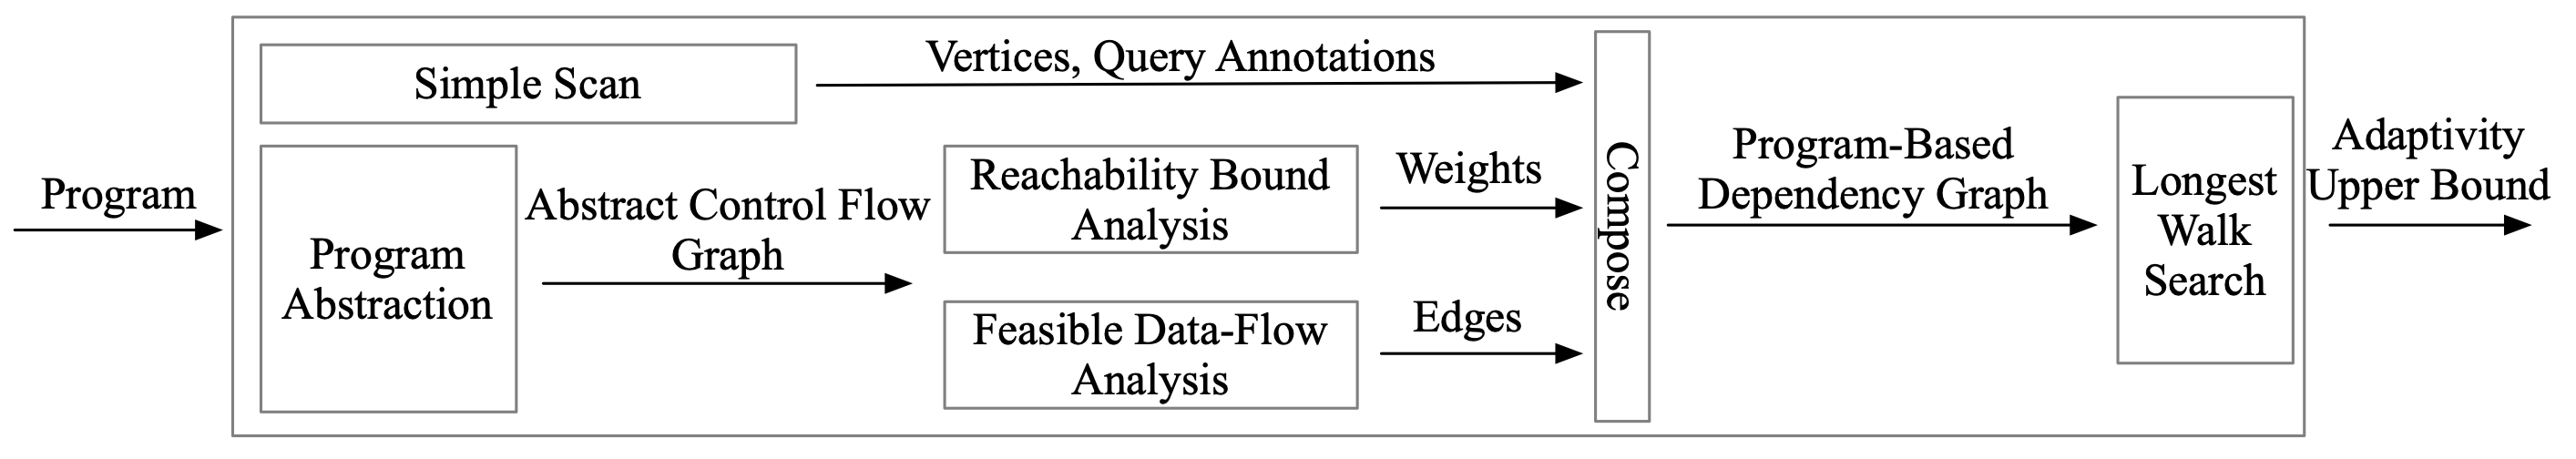
\includegraphics[width=1.0\columnwidth]{adapfun.png}
  \vspace{-0.3cm}
  \caption{The overview of {\THESYSTEM}}
  \label{fig:adaptfun}
  \vspace{-0.5cm}
\end{figure}

\begin{enumerate}
  % \item The data dependency relation analysis through the static data flow analysis technique.
  % \item The dependency quantity analysis through the static program reachability bound analysis techniques.
  % \item The program adaptivity estimation, through newly designed algorithms based on the results estimated above, 
  % computing the adaptivity upper bound soundly 
  % and accurately.
  \item \textbf{\emph{Dependency Relation} Estimation} in Section~\ref{sec:static-dep}.
  In order to accurately estimate the adaptivity,  {\THESYSTEM} first estimates
  %  the \emph{dependency relation} 
  %  Corresponding to the {\THESYSTEM} analyzes 
  the data \emph{dependency relation} through the static data flow analysis technique in Section~\ref{sec:static-dep}.
  This analysis step corresponds to the first step in execution-based adaptivity analysis. 
  The estimated result produced from 
  this step is proved as a sound upper bound for the variable \emph{may-dependency} relation in Definition~\ref{def:var_dep} from execution-based analysis in Section~\ref{sec:dynamic-datadep}.
  \item \textbf{\emph{Dependency Quantity} Estimation} in Section~\ref{sec:static-quantity}.
  % Still , 
  Corresponding to the second step in execution-based adaptivity analysis, {\THESYSTEM} then estimates the \emph{dependency quantity} 
  % is estimated by {\THESYSTEM} 
  through the static program reachability bound analysis techniques.
  %
  For every labeled variable and every pair of labeled variables with estimated dependency relation, this analysis provides the symbolic
 bounds on their reaching times during the program execution.
  % , in Section~\ref{sec:static-quantity}.
  % This analysis corresponds to the second step in execution-based adaptivity analysis. 
  The estimated result produced from 
  this step is proved as a sound upper bound for the reachability-bound from execution-based analysis as well.
  \item \textbf{\emph{Adaptivity} Estimation} in Section~\ref{sec:static-adapt}.
  % The program  estimation, 
  % In 
  The static program adaptivity analysis in this step
  % , specifically estimating 
  estimates the \emph{adaptivity} formalized in Definition~\ref{def:trace_adapt}, in following two steps:
  \begin{itemize}
  %  is presented in Section~\ref{sec:static-reachability}.
  % the program adaptivity estimation, 
  \item According to the third step of execution-based adaptivity analysis, 
  {\THESYSTEM} in this step first builds a similar graph to {over-}approximate the
  % execution-based dependency graph (in Definition~\ref{def:trace_graph})
  Execution-Based Dependency Graph (in Definition~\ref{def:trace_graph})
  \\
  This graph is built over the same vertices set as the execution-based dependency graph, which is program's set of labeled variables with unique labels.
  \\
  Then it builds the edges between vertices 
  % consider both control flow and data flow, generated in
  using the estimated dependency relation from Section~\ref{sec:static-dep}.
  % which is the same set as the vertices in the execution-based dependency graph extracted directly from the program
  %  constructs a program-based dependence graph for approximating the execution-based dependency graph.
  %  in Section~\ref{sec:dynamic-adapt}.
  \\
  Then according to the estimated reachability bound for every labeled variable and every pair of labeled variables with estimated dependency relation
  from Section~\ref{sec:static-quantity}, it assigns weight for every vertex and every edge on this graph.
  \\
  Overall, this program-based graph has a similar topology structure as 
  % the one
  % of 
  the Execution-Based Dependency Graph. It has the same
  vertices and query annotations, but approximated edges and weights. We call the graph generated by static analysis techniques, static analysis dependency graph. 
\item Then, based on this graph, {\THESYSTEM} 
    computes the adaptivity upper bound soundly 
    and accurately through a newly designed algorithm.
\\
Likewise, the adaptivity is defined as a finite walk in the execution based dependency graph, 
our static estimation on this adaptivity also relies on finding a path in the static analysis dependency graph.
The construction of the static analysis dependency graph is of great value of showing some useful properties of the target program,
such as dependency between variables, 
the execution upper bound of a certain command, while the key novelty is our path searching algorithm,
which connects all the information we need in the static analysis dependency graph and provides us a sound over-estimation of adaptivity! 
In order to get a sound but precise upper bound, 
we will discuss some challenges in finding the 'appropriate' path in the graph, 
and how our algorithm responds to these challenges.
I present the path searching algorithm in Section~\ref{sec:static-adapt}.
  \end{itemize}
  \end{enumerate}
% \subsubsection{Graph Estimation}
%
%
% According to the dependency graph we use in adaptivity definition, we want to build a similar graph to {over-}approximate the
% % execution-based dependency graph (in Definition~\ref{def:trace_graph})
% Execution-Based Dependency Graph (in Definition~\ref{def:trace_graph}). The construction considers the vertices, edges, and the weight of every node, as well as some annotations which marks the query usage. The overall picture of this step is organized as follows.
% % through Section~\ref{sec:alg_vertexgen}, Section~\ref{sec:alg_weightedgegen} and~\ref{sec:alg_graphgen}:


% \begin{enumerate}
% \item  Vertices are the program's labeled variables with unique labels,
% which is the same set as the vertices in the execution-based dependency graph extracted directly from the program
% % , see Section~\ref{sec:static-adapt}
% % without extra static analysis technique.
% % \item Query annotations are also decided directly from the program, when there is a query request, the associated variables which are the results of the query requests are marked in the form of a flag, $0$ means no query, $1$ represents query related. See Section~\ref{sec:alg_vertexgen}.
% \item The edges between vertices consider both control flow and data flow, generated in
% Section~\ref{sec:static-dep}
% \item Every 
% vertex has a weight, which tells the maximal times that this vertex can be reached in realistic execution.
% This weight is estimated by a reachability bound analysis on each vertex, See Section~\ref{sec:static-quantity}.
% \item Every 
% vertex has a weight, which tells the maximal times that this vertex can be reached in realistic execution.
% This weight is estimated by a reachability bound analysis on each vertex, See Section~\ref{sec:static-quantity}.

% \item  Finally, with all the ingredients ready, we construct the final approximated program-based dependency graph in Section~\ref{sec:static-adapt}
% \end{enumerate}

% % the algorithm  without extra static analysis technique.
% % \\
% Overall, this program-based graph has a similar topology structure as 
% % the one
% % of 
% the Execution-Based Dependency Graph. It has the same
% vertices and query annotations, but approximated edges and weights. We call the graph generated by static analysis techniques, static analysis dependency graph. 

% \subsubsection{Adaptivity Computation}

% Likewise the adaptivity is defined as a finite walk in the execution based dependency graph, 
% our static estimation on this adaptivity also relies on finding a path in the static analysis dependency graph.
% The construction of the stastic analysis dependency graph is of great value of showing some useful properties of the target program, such as dependency between variables, 
% the execution upper bound of a certian command, while the key novelty is our path searching algorithm, which connects all the information we need in the static analysis dependency graph and provides us a sound over-estimation of adaptivity! 
% In order to get a sound but precise upper bound, 
% we will discuss some challenges in finding the 'appropriate' path in the graph, and how our algorithm responds to these challenge. We present the path searching algorithm in Section~\ref{sec:static-adapt}.
In order to have a sound and accurate upper bound on the  adaptivity of a program $c$,
we design a program analysis framework named {\THESYSTEM}.
This framework composes two algorithms as shown in the double-stroke box and the dashed box in Fig.~\ref{fig:adaptfun}.
The first algorithm in the double-stroke box combines the quantitative and dependency analysis techniques.
It produces an estimated \emph{data-dependency graph} for a program.
The second algorithm in the dashed box is a walk length estimation algorithm.
%  in the dashed box in Fig.~\ref{fig:adaptfun}.
It computes the upper bound on the program's \emph{adaptivity} over the estimated graph.
%  of the adaptive data analysis program $c$.
\begin{figure}
  \centering    
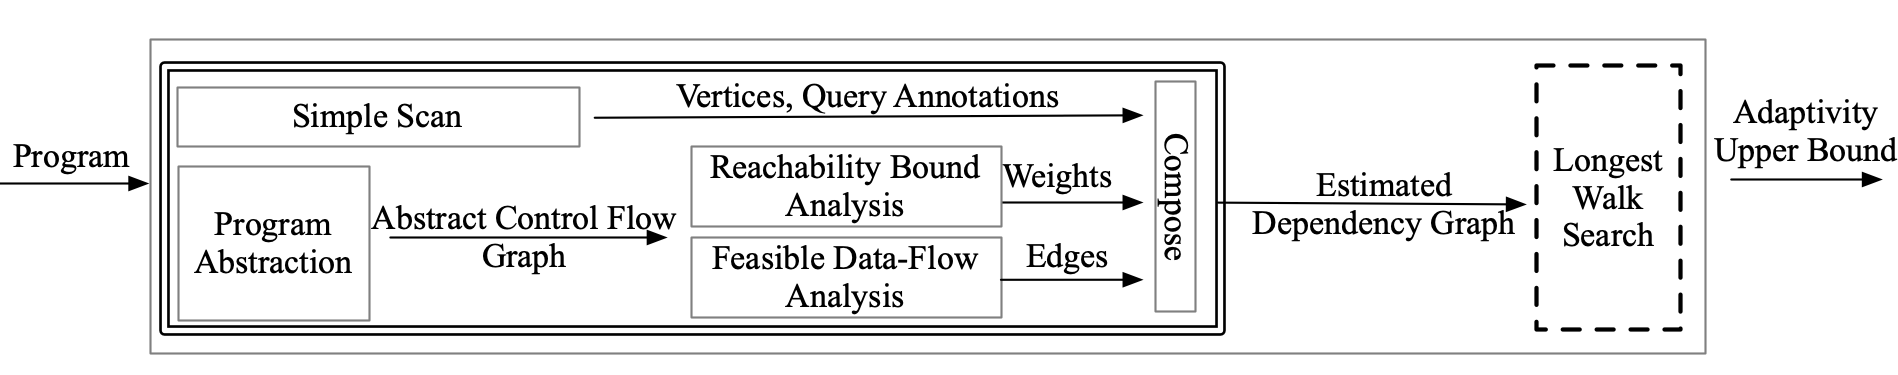
\includegraphics[width=1.0\columnwidth]{adaptfun.png}
  \vspace{-0.3cm}
  \caption{The overview of {\THESYSTEM}}
  \label{fig:adaptfun}
  \vspace{-0.5cm}
\end{figure}
%
Below is the outline of the {\THESYSTEM}.
% through Section~\ref{sec:alg_vertexgen}, Section~\ref{sec:alg_weightedgegen} and~\ref{sec:alg_graphgen}:
\begin{enumerate}
  \item \textbf{Graph Estimation}
  Because adaptivity is defined over a program's \emph{quantitative dependency graph} (in Definition~\ref{def:trace_graph}),
  this algorithm first estimates this graph for the program statically
  in Section~\ref{sec:alg_graphgen}.
  It estimates the four components of this graph in two steps and then composes them into an estimated dependency graph
  %  for a program 
  in the last step.
  The steps are summarized  as follows.
\begin{enumerate}
  \item \textbf{Vertex and Query Annotation Estimation}
  Vertices and query annotations in this graph are the assigned variables with unique labels. These are extracted directly from the program as in Section~\ref{sec:alg_vertexgen}.
  \item \textbf{Edge and Weight Estimation}
  \\
  This step estimates the edge and weight for a quantitative dependency graph. It combines the control, data-flow  analysis algorithm and the loop bound inference algorithm.
  There are three computation steps in this algorithm.
  \\
  \textbf{Abstract Control Flow Graph.}
  In order to perform the dependency analysis and quantitative analysis, this step first generates an \emph{abstract control flow graph} for a program in Section~\ref{sec:alg_abscfg}.
  \\
  \textbf{Edges Estimation via Combined Flow Analysis.} 
  The step is presented in
  Section~\ref{sec:alg_edgegen}. It performs over the \emph{abstract control flow graph}, which combines both control flow and data flow analysis.
  It estimates the \emph{dependency relation} between each pair of the labeled variables in a program by considering both the control flow and data flow.
  Then it uses the estimated dependency relation to approximate the edge
  %  of the quantitative dependency graph 
  between each pair of vertices.
  \\
  \textbf{Weights Estimation via Quantitative Analysis.} 
  This step is presented in Section~\ref{sec:alg_weightgen}. 
  It performs over the same \emph{abstract control flow graph} and computes the upper bound on the maximal visiting times of each labeled variable for a program.
  It estimates the reachability bound for every vertex over the \emph{abstract control flow graph},
  and this reachability bound is used to estimate the maximal visiting times of each labeled variable in a program and the weight of the corresponding vertex.
  %  of this quantitative dependency graph.
\item  \textbf{Graph Estimation.} 
In Section~\ref{sec:alg_graphgen}, we construct the final approximated graph,
named \emph{estimated dependency graph} by simply composing the four estimated ingredients. 
Overall, this \emph{estimated dependency graph} has a similar topology structure as 
the \emph{semantics-based dependency graph}. It has the same
vertices and query annotations, but approximated edges and weights. 
\end{enumerate}

\item \textbf{Adaptivity Computation.} 
Likewise the adaptivity in Definition~\ref{def:trace_adapt},
%  is defined as a finite walk in the \emph{semantics based dependency graph}, 
the static estimation on the \emph{adaptivity} also relies on finding a walk in the \emph{estimated dependency graph}.  
We discuss some challenges in finding the 'appropriate' walk in the graph, and how our algorithm responds to these challenges as
% . We present the path searching algorithm 
in Section~\ref{sec:alg_adaptcompute}.
\end{enumerate}


% \subsection{Static Data Dependency Analysis}
% \label{sec:static-dep}
% % %
\subsection{Base Steps for Static Data Dependency and Dependency Quantity Analysis}
\label{sec:alg_weightedgegen}
\subsubsection{Vertices Estimation and Query Annotation Estimation}
\label{sec:alg_vertexgen}
The vertices in the static analysis dependency graph are actually identical as the  Execution-Based Dependency Graph, which are assigned variables in the program annotated with the unique label(line number). These vertices are collected by statically scanning the program, like what I do for vertices of its Execution-Based Dependency Graph. The vertices are defined formally as follows.

  \highlight{
\[
    \progV(c) \triangleq \left\{ 
  x^l \in \mathcal{LV} 
  ~ \middle\vert ~
  x^l \in \lvar_{c}
  \right\}
  \]
  }
  %

The static scanning of the programs also tells us whether one vertice(assigned variable) is assigned by a query request.  I have similar definition when defining the Execution-Based Dependency Graph, 
a set of pairs $\progF(c) \in \mathcal{P}(\mathcal{LV} \times \{0, 1\} )$ 
% is the set of pairs 
% The weight for each vertex in $\progV(c)$ is computed 
mapping each $x^l \in \progV(c)$ to a flag, either $0$ or $1$, where $1$  means $x^{l}$ is a member of $ \qvar_{c}$, a set of those variables assigned with query requests, and $0$ means $x^{l}$ not in this set. It is defined formally below.

\[\progF(c) =\left\{(x^l, n)  \in  \mathcal{LV} \times \{0, 1\} 
~ \middle\vert ~
x^l \in \lvar_{c},
n = 1 \iff x^l \in \qvar_{c} \land n = 0 \iff  x^l \not\in \qvar_{c} .
\right\}\]
%
\subsubsection{Abstract Execution Control Flow graph}
Since the edges of the execution-based graph of a program relies on the dependency relation, which handles both control flow and data flow, as an over-approximation of this graph, the edges of our static anlaysis dependency graph also covers these two kind of flows.  I develop a feasible data flow relation to catch these two flows, in Section~\ref{sec:alg_edgegen}.
%
The weight of every vertice in the execution-based graph is built on all possible execution traces.
In order to over-approximate the weight statically but still tightly, I present a symbolic reachability bound analysis for estimation of the weight of each vertice(label) in Section~\ref{sec:alg_weightgen},
in spirit of some reachablility bound techiniques.


The edges and weight estimation are both performed on basis of an abstract control flow graph of the program, I first show how to generate this abstract execution control flow graph before the introduction of  the edge and weight estimation.  
\label{sec:abscfg}
 I discuss the vertices and edge of the
abstract control flow graph for a program $c$, $\absG(c)$.

Every 
vertex corresponds to the unique
label.
Specifically,
the vertices of this graph is the set of $c$'s labels with an exit label $l_{ex}$, 
\[ 
  \absV(c) = labels(c)\cup\{l_{ex}\}
  \]
%  corresponding to a label command in the program.

% \wq{
  The edge in the abstract control flow graph comes from the abstract execution trace of the program. 
  The abstract execution trace, an abstract representation of the execution, consists of a list of abstract transitions. 
  Then, every abstract transition in the abstraction execution trace corresponds to an edge in the abstract control flow graph. In another word, the edge $(l_1, dc, l_2)$ in the abstract control flow graph, represents an abstract transition 
 from $l_1$ to $l_2$, with a set of difference constraints $dc$. 
 Also notice, the difference constraints generated during the abstract transition appears in the edge as annotation.
%  }

% over program's abstract execution 


% \wq{
  Overall, the vertices can be easily collected and the key point of construction of the abstract execution control flow graph for a program is the abstract execution trace, 
  which relies on the abstraction of expression and abstract transition (we also call it abstract event), I will discuss in the following section.
   To make it easy to understand, abstract control flow graph is a control flow graph, with difference constraints on every edge.
  % }  

%
\paragraph*{Expression Abstraction}

The expression assigned to the variable on the left hand of the assignment command is abstracted to an abstract value: (adopted from the expression abstraction method in paper \cite{sinn2017complexity}). The abstract value is expressed in the form of Difference constraint, denotated as $DC : \mathcal{VAR} \cup \constdom \to \mathcal{\mathcal{VAR} \times (\mathcal{VAR} \cup \constdom) } \times (\mathbb{Z} \cup \{\infty\})$.  $\constdom$ is called the Symbolic Constant defined as $\constdom \triangleq \mathbb{N} \cup \inpvar \cup \{\max{(\dbdom)}\} $, which consists of 
natural numbers $\mathbb{N}$,
the program's input variables $\inpvar$  
and a constant value $\max(\dbdom)$ for estimating the upper bound of variables which are
assigned by queries. 

Give an instance of difference constraint used here,
$DC(\mathcal{VAR}  \cup \constdom) \cup \{\top\}$ represents all the difference constraints over 
variable and symbolic constants. 
% The difference constraint $DC$ over $\mathcal{VAR} \cup \constdom$ 
It is a set of the inequality of form $x \leq y + v$ where $x \in \mathcal{VAR} $, 
$y \in \mathcal{VAR}  \cup \constdom$ and $v \in \mathbb{Z}$. 
This difference constraint is defined in the same way as
\cite{sinn2017complexity}. For concise, I use $\dcdom^{\top}$ to represent the $DC(\mathcal{VAR}  \cup \constdom) \cup \{\top\}$ .


 I show the expression abstraction $\absexpr : \expr \to \mathcal{VAR} \to DC(\mathcal{VAR}  \cup \constdom) \cup \{\top\} $ below.

%  I introduce the following notations and operations first
% % an expression abstraction method based on the expression abstraction in paper \cite{sinn2017complexity}.
% \\
% % is enriched into $\constdom \triangleq \mathbb{N} \cup \inpvar \cup \{\max{(\dbdom)}\} $.
% T
% \\

% represents the set of inequality over all $\mathcal{VAR}  \cup \constdom$. 

% The symbolic constant is enriched into $\constdom \triangleq \mathbb{N} \cup \inpvar \cup \{\max{(\dbdom)}\} $.
% It consists of 
% natural number $\mathbb{N}$,
% the symbolic constants $\inpvar$ (i.e., the set of the program's input variables), 
% and a constant value $\max(\dbdom)$ for estimating the upper bound of variables which are
% assigned by queries.
% \\
% The symbolic constant is enriched into $\constdom \triangleq \mathbb{N} \cup \inpvar \cup \{\max{(\dbdom)}\} $.
% \\

% % $ \absdom: \mathcal{P}(DC(\mathcal{VAR}  \cup \constdom) \cup \{\top \})$:
% \\
% $\constdom: \mathbb{N} \cup \inpvar \cup \{\max{(\dbdom)}\} $ 
% The  constant 
% \\
% % $DC(\mathcal{VAR}  \cup \constdom)$ represents the set of inequality over all $\mathcal{VAR}  \cup \constdom$.
% \\

% \[
%   \begin{array}{ll} 
%     \absexpr(y + c, x)  = x' \leq y + c  & c \in \mathbb{N} \land y \in (VAR \cup \constdom) \\
%     \absexpr(y - c, x)  = x' \leq y - c  & c \in \mathbb{N} \land y \in (VAR \cup \constdom) \\
%     \absexpr(v, x)  = x' \leq v + 0  & v \in (VAR \cup \constdom) \\
%     \absexpr(\aexpr, x) = x' \leq 0 + \infty   & \aexpr \text{ doesn't have any of the forms as above} \\
%     \absexpr(\qexpr, x)  = x' \leq 0 + \max(\dbdom) & \qexpr \text{ is a query expression}  \\
%     \absexpr(\bexpr, x) = x' \leq 0 + 1   & \bexpr \text{ is a boolean expression} \\
%   \end{array}
%   \]
  \[
    \begin{array}{ll} 
      \absexpr(x - v, x)  = x' \leq x - v  & x \in \grdvar \land v \in \mathbb{N} \\
      \absexpr(y + v, x)  = x' \leq y + v  & x \in \grdvar \land v \in \mathbb{Z} \land y \in (\grdvar \cup \constdom) \\
      \absexpr(v, x)  = x' \leq v + 0  & x \in \grdvar \land v \in (\grdvar \cup \constdom) \\
      \absexpr(y + v, x)  = x' \leq y + v & \\
      \grdvar = \grdvar \cup \{y\} & x \in \grdvar \land v \in \mathbb{Z} \land y \notin (\grdvar \cup \constdom)  \\
      \absexpr(\qexpr, x)  = x' \leq 0 + \max(\dbdom) & x \in \grdvar \land \qexpr \text{ is a query expression}  \\
      \absexpr(\bexpr, x) = x' \leq 0 + 1   & x \in \grdvar \land \bexpr \text{ is a boolean expression} \\
      \absexpr(\expr, x) = x' \leq \infty  &  x \in \grdvar \land \expr \text{ doesn't have any of the forms as above} \\
      \absexpr(\expr, x) = \top  &  x \notin \grdvar \\
    \end{array}
    \]
  
  % \wq{ 
    $\grdvar$ is the set of variables used in the guard expression of every while command in the program $c$. 
  % }. 
  In the case 4, if a variable $x$, belonging to the set 
  $\grdvar$ is updated by a variable $y$, which isn't in this set, 
  I add $y$ into the set $\grdvar$ and repeat 
  above procedure  until $\grdvar$ and $\absexpr(\expr, x)$ is stabilized. 
  % \wq{I do not understand this sentence:-(}
  \\
Specifically 
% understanding the intuition, 
we handle a 
% simplified 
normalized guard expression ($ x > 0$ for $x^l \in \lvar_c$)
 in $\ewhile$, and 
%  \wq{I do not understand this sentence:-(}
%  .
% \\
% The counter variables only increase, decrease or reset by expression in the form of arithmetic minus and plus (able to extend to max and min.)
the counter variables only increase, decrease or reset by 
% expression in the form of 
simple arithmetic expression (mainly multiplication, division, minus and plus (able to extend to max and min)). 
This is the same as in paper \cite{sinn2017complexity}. 
\\
For more complex expression assignments, where the counter reset, or calculated from $\elog$, 
multiplication or division, and expressions involving multiple variables, the constraint is approximated as reset of $\infty$.
\\
% This simplification \wq{which part I simplify here?} 
This approximation strategy
doesn't affect our analysis results in our examples. It is easy to extend the normalized expression 
into more complex forms as in \cite{sinn2017complexity}, as well as the 
counter variable manipulation with more advanced expressions.
% \\ 
% The boolean expression in the guard of $\ewhile$ command is normalized into form of $ x > 0$ where $x^l \in \lvar_c$ for some $l$.


\paragraph{Program Event Abstraction}
 I show the abstract event definition, which is generated when computing its abstract execution trace.

\begin{defn}[Abstract Event]
  \label{def:abs_event}
  Abstract Event: 
  $\absevent \in $
  $\ldom \times \dcdom^{\top} \times \ldom$
  is a 
  % pair of abstract initial state and final state.
  triple where the first and third components are labels,
  second component is a constraint from $\dcdom^{\top}$.
  % the thrid % computed from program's abstract final and initial state, $\absfinal(c)$ and $\absinit(c)$ with formal definition, and algorithm detail in Appendix.
  %  the constraint and the third corresponds to a final state.
  \end{defn}
  Specifically, in an abstract event, 
  the first label correspond to an initial state, and 
  the second label and the constraint correspond to an abstract final state.
 The abstract initial state is a label from $\ldom$.
The abstract final state is a pair from $\ldom \times \dcdom^{\top}$,  
where first component is a label from $\ldom$ and the second component is a constraint from $\dcdom^{\top}$.
%

%
Given a program $c$, its abstract initial state,
and the set of its abstract final state is computed as follows,
%
\[
  \begin{array}{ll}
    \absinit(\clabel{\assign{x}{\expr}}{}^l)  & = l  \\
    \absinit(\clabel{\assign{x}{\expr}}{}^l)  & = l \\
    \absinit(\clabel{\eskip}^{l})  & = l \\
    \absinit(\eif [b]^l \ethen c_1 \eelse c_2)  & = l \\
    \absinit(\ewhile [b]^l \edo c)  & = l \\
    \absinit(c_1 ; c_2)  & = \absinit(c_1) \\
 \end{array}
 \]
%
Final State Abstraction: 
$\absfinal: \cdom \to \mathcal{P}(\ldom \times \dcdom^{\top})$,
computes the set of Abstract Final State for the command. 
 \[
  \begin{array}{ll}
    \absfinal(\clabel{\assign{x}{\expr}}{}^l)  & = \{(l, \absexpr\eapp (\expr, x))\}  \\
     \absfinal(\clabel{\assign{x}{\query(\qexpr)}}{}^l)  & = \{
      (l, x' \leq 0 + \max(\dbdom) )\}  \\
     \absfinal(\clabel{\eskip}^{l})  
     & = \{(l, \top)\} \\
     \absfinal(\eif [b]^l \ethen c_1 \eelse c_2)  & = \absfinal(c_1) \cup \absfinal(c_2) \\
     \absfinal(\ewhile [b]^l \edo c)  & = \{(l, \top)\} \\
     \absfinal(c_1 ; c_2)  & =  \absfinal(c_2) \\
 \end{array}
 \]
 %
 \paragraph{Abstract Execution Trace}
 Now, I  extract the abstract execution trace  $\absflow(c)$ for a program, which computes the Abstract Execution Trace for program $c$, as a set of the abstract events $\absevent$.
 %
 \begin{defn}[Abstract Execution Trace]
 \label{def:abs_trace}
  $\absflow \in \cdom \to \mathcal{P}( \ldom \times DC(\mathcal{VAR}  \cup \constdom) \cup \{\top\}) \times \ldom )$
  \end{defn}
 %

 
   I now show how to compute the abstract execution trace. 
  For simplicity, I use $\mathcal{P}(\absevent)$ represent the power set of all abstract events, and I have $\absflow(c) \in \mathcal{P}(\absevent)$.
  I first append a skip command with 
%  a symbolic label $l_e$, i.e., $\clabel{\eskip}^{l_e}$ at the end of the program $c$, and compute the $\absflow(c) = \absflow'(c')$ for $c'$, where $c' = c;\clabel{\eskip}^{l_e}$ as follows,
the exist label $l_{ex}$, i.e., $\clabel{\eskip}^{l_{ex}}$ at the end of the program $c$, 
and compute the $\absflow(c) = \absflow'(c')$ for $c'$, where $c' = c;\clabel{\eskip}^{l_{ex}}$ as follows,
 %
 {\footnotesize
 \[
   \begin{array}{ll}
      \absflow'(\clabel{\assign{x}{\expr}}{}^l)  & = \emptyset  \\
      \absflow'(\clabel{\assign{x}{\query(\qexpr)}}{}^l)  & = \emptyset  \\
      \absflow'([\eskip]^{l})  & = \emptyset \\
      \absflow'(\eif [b]^l \ethen c_t \eelse c_f)  & =  \absflow'(c_t) \cup \absflow'(c_f)
      %   \\ & \quad 
        \cup \{(l, \top,  \absinit(c_t) ) ,  (l, \top, \absinit(c_f)) \} \\
       \absflow'(\ewhile [b]^l \edo c_w)  & =  \absflow'(c_w) \cup \{(l, \top, \absinit(c_w)) \} 
      %  \\ & \quad 
       \cup \{(l', dc, l)| (l', dc) \in \absfinal(c_w) \} \\
       \absflow'(c_1 ; c_2)  & = \absflow'(c_1) \cup  \absflow'(c_2) 
      %  \\ & \quad 
       \cup \{ (l, dc, \absinit(c_2)) | (l, dc) \in \absfinal(c_1) \} \\
   \end{array}
   \]
   }

   Notice $\absflow'([x := \expr]^{l})$, $\absflow'([x := \query(\qexpr)]^{l})$ and $\absflow'([\eskip]^{l})$ are all empty set. 
   For every event $\event$ with label $l$ in an execution trace $\trace$ of program $c$, 
   there is an abstract event in program's abstract execution trace of form $(l, \_, \_)$.  
    I also show the soundness of the abstract execution trace in Appendix.
  %  which says 
  %  \wq{...}
   \begin{lem}[Soundness of the Abstract Execution Trace]
     \label{lem:abscfg_sound}
   Given a program ${c}$, I have:
   %
   \[
     \begin{array}{l}
       \forall \vtrace_0, \trace \in \mathcal{T} ,  \event = (\_, l, \_) \in \eventset \sthat 
   \config{{c}, \trace_0} \to^{*} \config{\eskip, \trace_0 \tracecat \vtrace} 
   \land \event \in \trace 
   \\
   \qquad \implies \exists \absevent = (l, \_, \_) \in (\ldom\times \dcdom^{\top} \times \ldom) \sthat  
   \absevent \in \absflow(c)
   \end{array}
   \]
   \end{lem}
%    This lemma is proved formally in Appendix~\ref{apdx:reachability_soundness}.
% For every event $\event$ with label $l$ in an execution trace $\trace$ of program $c$, 
% there is an abstract event in program's abstract execution trace of form $(l, \_, \_)$. 
This lemma is proved formally in Lemma~\ref{lem:abscfg_sound} in Appendix~\ref{apdx:reachability_soundness}.
\\
For every labeled variable in program $c$, $x^l \in \lvar_c$, there is a unique abstract event in program's abstract execution trace $\absevent \in \absflow(c)$ of form $(l, \_, \_)$. 
\begin{lem}[Uniqueness of the Abstract Execution Trace]
  \label{lem:abscfg_unique}
Given a program ${c}$, I have:
%
\[
  \begin{array}{l}
    \forall \vtrace_0, \trace \in \mathcal{T} ,  \event = (\_, l, \_, \_) \in \eventset^{\asn} \sthat 
\config{{c}, \trace_0} \to^{*} \config{\eskip, \trace_0 \tracecat \vtrace} 
\land \event \in \trace 
\\
\qquad \implies \exists! \absevent = (l, \_, \_) \in (\ldom\times \dcdom^{\top} \times \ldom) \sthat  
\absevent \in \absflow(c)
\end{array}
\]
\end{lem}
This lemma and proof is also 
formalized in Lemma~\ref{lem:absevent_unique} in Appendix~\ref{apdx:reachability_soundness}.

Then, I build the edge for $c$'s abstract control flow graph as follos,
\[
  \absE(c) = \{(l_1, dc, l_2) | (l_1, dc, l_2) \in \absflow(c)\}
  \]

%  I have a pre-processing algorithm to go through the programs and returns the list of labels associating with a loop and whose visiting times need to be analyzed.
%


\paragraph{Abstract Control Flow Graph} 
With the vertices $\absV(c)$ and edges $\absE(c)$ ready, I construct the abstract control flow graph, formally 
% Through a program $c$'s abstract execution trace, its abstract control flow graph is computed 
defined in 
Definition~\ref{def:abs_cfg}.
% Given program $c$ with its abstract control flow $\absflow(c)$, the Abstract Control Flow Graph:
% \\
\begin{defn}[Abstract Control Flow Graph]
\label{def:abs_cfg}
Given a program $c$, 
with its abstract control flow $\absflow(c)$
its abstract control flow graph $\absG(c) =(\absV(c), \absE(c), \absW(c))$ is defined as follows,
\\
% \highlight{
% :
%
% \\
$\absE(c) = \{(l_1, dc, l_2) | (l_1, dc, l_2) \in \absflow(c)\}$,
\\
$\absV(c) = labels(c)\cup\{l_{ex}\}$
\\
 $\absW(c) 
\triangleq \left\{ (l, w) \in \mathbb{L} \times EXPR(\constdom) \right\}$.
% }
% \\
% , where the weight of every label to be computed in the next step.
\end{defn}
% 
% The vertices $\absV(c)$ in this graph are program's labels with an exit label $l_{ex}$.
% Each directed 
%  edge $(l_1, dc, l_2)$ from $l_1$ to $l_2$,
%  represents an abstract transition 
%  between two control locations with a set of difference constraints on it.
% %  , i.e., the labels of two commands (we call the labels also control location and they refer to the same thing), 
% %  where 
% In this transition, the  command labeled with the second location $l_2$, 
%  will be executed after execution of the command with label $l_1$,
% %  The abstract transition contains a set of difference constraints for variables, 
% with the difference constraints generated by abstracting the command of the first label.
% % \\
% % It is easy to show for every $(l_1, dc, l_2) \in \absflow(c)$ such that $l_2 \neq l_e$, $(l_1, l_2) \in flow(c)$. The formal Lemma and proof can be found in Lemma~\ref{lem:flow_to_absflow} in Appendix~\ref{apdx:reachability_soundness}.
Notice I also define the $\absW(c)$ in this graph without giving an actual value.
This $\absW(c)$ is the set of weight for every 
% vertex 
label. The weight is a symbolic expression over the symbolic constant, 
which is the estimated upper bound on the number of visiting time for every control location
through the reachability bound analysis as follows.
%
% It is easy to show for every $(l_1, dc, l_2) \in \absflow(c)$ such that $l_2 \neq l_e$, $(l_1, l_2) \in flow(c)$. The formal Lemma and proof can be found in Lemma~\ref{lem:flow_to_absflow} in Appendix~\ref{apdx:reachability_soundness}.
%
\paragraph*{Abstract Control Flow Graph Through An Example}
%
\begin{example}[The Abstract Control Flow Graph for Two Rounds Data Analysis Program Example]
    For the same two adaptivity rounds example program, 
its generated abstract control flow graph is shown as in Figure~\ref{fig:abscfg_tworound}(b).
For example, the edge $(0, a \leq 0, 1)$ on the top, tells us the command 
$\clabel{\assign{a}{0}}^0$ is executed with next continuation location $1$,
where the 
command $\clabel{\assign{j}{k}}^1$ will be executed next.
The constraint $a \leq 0$ is a difference constraint, generated by abstracting from the assignment command $\assign{a}{0}$,
representing that value of $a$ is less than or equals to $0$ after 
location $0$ before executing command at line $1$. The difference constraint is an inequality relation between, the left-hand side of the inequality talks about the variable before the execution and the right-hand side ascribes those after the execution. 
Look at the $a < a+x $ on the edge $5$ to $2$, which describes the execution of the command at line $5$, which is an assignment $a = a+x$. The $a$ on the left side of $a < a+x$ represents the value of $a$ after the assignment, while the right-hand side $a$ stores the value before the assignment. 
Also, I have while loop, which is a circle $2 \to 4 \to 5 \to 2$ in Figure~\ref{fig:abscfg_tworound}(b). 
Please also look at the edge from $3$ to $4$, which talks about the query! The $x < \max(\dbdom)$ describes the execution of a query request (the command at line 3), the query results stored in $x$ is bounded by $\max(\dbdom)$. 
$\max(\dbdom)$ is the maximal value for query requesting result from the database $DB$. $top$ means there is no assignment executed, for example, I have the difference constraint $\top$ on the edge $2$ to $6$, means at line $2$, there is no assignment (it is a testing guard $j>0$.) 
%
The same way for the rest edges' constructions.
\begin{figure} 
  \centering
  \begin{subfigure}{.7\textwidth}
  \begin{centering}
  {\small
  $
      \begin{array}{l}
            \clabel{ \assign{a}{0}}^{0} ;   
              \clabel{\assign{j}{k} }^{1} ;\\
              \ewhile ~ \clabel{j > 0}^{2} ~ \edo ~ 
              \Big(
               \clabel{\assign{x}{\query(\chi[j])} }^{3}  ;
               \clabel{\assign{j}{j-1}}^{4} ;
              \clabel{\assign{a}{x + a}}^{5}       \Big);\\
              \clabel{\assign{l}{\query(\chi[k]*a)} }^{6}
          \end{array}
  $
  }
  \caption{}
  \end{centering}
  \end{subfigure}
    \begin{subfigure}{.45\textwidth}
    \begin{centering}
  %   \todo{abstract-cfg for two round}
  \begin{tikzpicture}[scale=\textwidth/20cm,samples=200]
  \draw[] (-7, 10) circle (0pt) node{{ $0$}};
  \draw[] (0, 10) circle (0pt) node{{ $1$}};
  \draw[] (0, 7) circle (0pt) node{\textbf{$2$}};
  \draw[] (0, 4) circle (0pt) node{{ $3$}};
  \draw[] (0, 1) circle (0pt) node{{ $4$}};
  \draw[] (-7, 1) circle (0pt) node{{ $5$}};
  % Counter Variables
  \draw[] (6, 7) circle (0pt) node {\textbf{$6$}};
  \draw[] (6, 4) circle (0pt) node {{ $ex$}};
  %
  % Control Flow Edges:
  \draw[ thick, -latex] (-6, 10)  -- node [above] {$a \leq 0$}(-0.5, 10);
  \draw[ thick, -latex] (0, 9.5)  -- node [left] {$j \leq k$} (0, 7.5) ;
  \draw[ thick, -latex] (0, 6.5)  -- node [left] {$\top$}  (0, 4.5);
  \draw[ thick, -latex] (0, 3.5)  -- node [right] {$x \leq Q_m$} (0, 1.5) ;
  \draw[ thick, -latex] (-0.5, 1)  -- node [above] {$j \leq j - 1$} (-6, 1) ;
  \draw[ thick, -latex] (-6, 1.5)  -- node [left] {$a \leq a + x$} (-0.5, 7)  ;
  \draw[ thick, -latex] (0.5, 7)  -- node [above] {$l \leq Q_m$}  (5.5, 7);
  \draw[ thick, -latex] (6, 6.5)  -- node [right] {$\top$} (6, 4.5) ;
  \end{tikzpicture}
  \caption{}
    \end{centering}
    \end{subfigure}
    \begin{subfigure}{.45\textwidth}
      \begin{centering}
    %   \todo{abstract-cfg for two round}
    \begin{tikzpicture}[scale=\textwidth/20cm,samples=200]
    \draw[] (-10, 10) circle (0pt) node{{ $0: 1$}};
    \draw[] (0, 10) circle (0pt) node{{ $1: 1$}};
    \draw[] (0, 7) circle (0pt) node{\textbf{$2: k$}};
    \draw[] (0, 4) circle (0pt) node{{ $3: k$}};
    \draw[] (0, 1) circle (0pt) node{{ $4: k$}};
    \draw[] (-10, 1) circle (0pt) node{{ $5: k$}};
    % Counter Variables
    \draw[] (6, 7) circle (0pt) node {\textbf{$6: 1$}};
    \draw[] (6, 4) circle (0pt) node {{ $ex: 1$}};
    %
    % Control Flow Edges:
  \draw[ thick, -latex] (-8, 10)  -- node [above] {$a \leq 0$}(-1.5, 10);
  \draw[ thick, -latex] (0, 9.5)  -- node [left] {$j \leq k$} (0, 7.5) ;
  \draw[ thick, -latex] (0, 6.5)  -- node [left] {$\top$}  (0, 4.5);
  \draw[ thick, -latex] (0, 3.5)  -- node [right] {$x \leq Q_m$} (0, 1.5) ;
  \draw[ thick, -latex] (-1.5, 1)  -- node [above] {$j \leq j - 1$} (-8, 1) ;
  \draw[ thick, -latex] (-8, 1.5)  -- node [left] {$a \leq a + x$} (-1.5, 7)  ;
  \draw[ thick, -latex] (1.5, 7)  -- node [above] {$l \leq Q_m$}  (4.5, 7);
  \draw[ thick, -latex] (6, 6.5)  -- node [right] {$\top$} (6, 4.5) ;
    \end{tikzpicture}
    \caption{}
      \end{centering}
      \end{subfigure}
    \caption{(a) The same $\kw{towRounds(k)}$ program as Figure~\ref{fig:twoRounds_example}
    (b) The abstract control flow graph for $\kw{towRounds(k)}$  (c) The abstract control flow graph with the reachability bound for $\kw{towRounds(k)}$.}
    \vspace{-0.5cm}
    \label{fig:abscfg_tworound}
  \end{figure}
\end{example}
%
% In order to estimate weight for every vertex in $\progV(c)$,
%  I first show how to compute the reachability bound for every label in $c$
%  % (i.e., every vertex in $\absV(c)$)
%  (i.e., the $\absW(c)$), 
%  then show how to compute the weight for every vertex in $\progV(c)$.
%  \\
%  Through the edges in $\absG(c)$, which correspond to $c$'s abstract transition between labels,

%  \wq{In order to estimate weight for every vertex in the static analysis dependency graph($\progV(c)$), I want to find out the upper bound on 
%  the number of times the labeled command (uniquely associated with a vertex in $\progV(c)$) may be executed when running the program.
%  This information can be obtained by computing the reachability bound for every vertice in the abstract control flow graph ($\absW(c)$), because
%  the vertices in the two graph share the same unique label, the line number.  I can easily show that the reachability bound on one vertex of the actract control flow graph is also the upper bound for the corresponding vertex in the static analysis dependency graph, both vertices share the same unique line number.}



%   I perform the symbolic reachability bound anaysis on the abstract control flow graph, 
%  through the edges in $\absG(c)$, which correspond to $c$'s abstract transition between labels.
%  I infer the invariant for every variable, and compute the transition closure for every abstract transition. By solving the closure
%  with the invariants of variables involved in this closure for every transition, I compute
%  the symbolic reachability bound of every commands corresponding to this transition.
%  \\
%  Specifically in four steps, Variable Modification Tracking, Local Bounds Computation,
%  the symbolic reachability bound of every commands corresponding to this transition. Specifically, this analysis can be performed in four steps:
%   Variable Modification Tracking, Local Bounds Computation,
%  Invariant Inference and Closure Generation, and Reachability Bound Computation,
{In order to estimate weight for every vertex in the static analysis dependency graph($\progV(c)$), I want to find out the upper bound on 
the number of times the labeled command (uniquely associated with a vertex in $\progV(c)$) may be executed when running the program.
This information can be obtained by computing the reachability bound for every vertex in the abstract control flow graph ($\absW(c)$), because
the vertices in the two graph share the same unique label, the line number.  I can easily show that the reachability bound on one vertex of the abstract control flow graph is also the upper bound for the corresponding vertex in the static analysis dependency graph, both vertices share the same unique line number.}


 I perform the symbolic reachability bound analysis on the abstract control flow graph, 
through the edges in $\absG(c)$, which correspond to $c$'s abstract transition between labels.
 I infer the invariant for every variable, and compute the transition closure for every abstract transition. By solving the closure
with the invariants of variables involved in this closure for every transition, I compute
the symbolic reachability bound of every commands corresponding to this transition. Specifically, this analysis can be performed in four steps:
 Variable Modification Tracking, Local Bounds Computation,
Invariant Inference and Closure Generation, and Reachability Bound Computation,
% 
%  I present the details of invariant, closure generation, and reachability bound computation as follows.
with details as follows.
%
%
\paragraph*{Variable Modification Tracking}
Identify the abstract events where each variable is increased, decreased and reset:
\\
$\inc: \mathcal{VAR} \to \mathcal{P}(\absevent) $
the set of the abstract events where the variable increase.
\\
$\inc(x) = \{(\absevent, c) | \absevent = (l, l', x' \leq x + v)\}$
\\
$\reset: \mathcal{VAR} \to \mathcal{P}(\absevent) $
The set of the abstract events where the variable is reset.
\\
$\dec: \mathcal{VAR} \to \mathcal{P}(\absevent) $
The set of abstract events where the variable decrease.
% \\
% $\dec(x) = \{(\absevent, c) | \absevent = (l, l', x' \leq x - v)\}$
\\
$Incr(v) \triangleq \sum\limits_{(\absevent, c) \in \inc(v)}\{\absclr(\absevent) \times v\}$
%
\paragraph*{Local Bounds}
Given a program $c$ with its abstract control flow graph 
$\absG(c) = (\absV, \absE)$
\\
Local Bounds Computation:
$\locbound: \absevent \to \mathcal{VAR} \cup \constdom$.
%
\[ 
\begin{array}{ll}
  \locbound(\absevent) \triangleq 1 
  & \absevent \notin SCC(\absG(c))
  \\
  \locbound(\absevent) \triangleq (x, v) 
  & \absevent \in SCC(\absG(c)) \land \absevent \in \dec(x) \land  \absevent = (\_, \_ , x' \leq x - v) \\
  \locbound(\absevent) \triangleq (x, \max(\dec(x))) 
  & \absevent \in SCC(\absG(c)) \land 
  \absevent  \notin \bigcup_{x \in \mathcal{VAR}} \dec(x)
  \land \absevent \notin SCC(\absG(c) \setminus \dec(x)) 
\end{array}
  \]
  The first case is straightforward. Since variable's visiting time outside of any while loop is at most 1, I do not need to analyze the visiting times of every node in the graph from phase 1.
  The second and third step is guaranteed by the \emph{Discussion on Soundness} in Section 4 of \cite{sinn2017complexity}.
  Then soundness proof is in Lemma~\ref{lem:local_bound_sound} in Appendix~\ref{apdx:reachability_soundness}.
%
\paragraph*{Invariant Inference and Closure Generation }
Then, computing the bound invariants for variables and the transition closures for abstract events:
\\ 
$ \varinvar: \mathcal{VAR} \cup \constdom \to EXPR(\constdom)$
\\
$\absclr: \absevent \to EXPR(\constdom)$
\\
Then, the symbolic invariant for each variable 
as well as the symbolic transition closure for each transition is calculated as follows:
\[ 
\begin{array}{lll}
  \varinvar(x) & \triangleq c & c \in \constdom \\
  \varinvar(x) & \triangleq Incr(v) + \max(\{\varinvar(a) + c | (t, a, c) \in \reset(x)\}) & c \notin \constdom
\end{array}
\]
%
\begin{defn}
  \label{def:transition_closure_base}
\[ 
\begin{array}{lll}
  \absclr(\absevent) 
  & \triangleq x / v & \\ 
  & \locbound(\absevent) = (x, v) \in \constdom \times \mathbb{N} & \\
  \absclr(\absevent) 
  & \triangleq (Incr(x) + 
  \sum\limits_{(\absevent', y, v') \in \reset(x)}
  \absclr(\absevent') \times \max(\varinvar(y) + v', 0) ) / v & \\
  & \locbound(\absevent) = (x, v) \land x \notin \constdom & 
\end{array}
  \]
\end{defn}
%
\paragraph*{Improved Variable Modification Tracking}
Instead of just identifying the abstract events where each variable is reset,
this improvement identifies the chain of the events where a given variable is reset by the 
variables of the abstract events through the chain.
\\
$\resetchain: \mathcal{VAR} \to \mathcal{P}(\mathcal{P}(\absevent)) $
The set of the chain of abstract events where the variable is reset through the chain.
% \\
% $Incr(v) \triangleq \sum\limits_{(\absevent, c) \in \inc(v)}\{\absclr(\absevent) \times v\}$
%
\paragraph*{Improved Invariant Inference and Closure Generation}
Then, computing the bound invariants for variables and the transition closures for abstract events:
\\ 
$ \varinvar: \mathcal{VAR} \cup \constdom \to EXPR(\constdom)$
\\
$\absclr: \absevent \to EXPR(\constdom)$
\\
Then, the symbolic invariant for each variable 
as well as the symbolic transition closure for each transition is calculated as follows:
\[ 
\begin{array}{lll}
  \varinvar(x) & \triangleq c & c \in \constdom \\
  \varinvar(x) & \triangleq Incr(v) + \max(\{\varinvar(a) + c | (t, a, c) \in \reset(x)\}) & c \notin \constdom
\end{array}
\]
%
\begin{defn}
  \label{def:transition_closure}
\[ 
\begin{array}{lll}
  \absclr(\absevent) 
  & \triangleq x / v & \\ 
  & \locbound(\absevent) = (x, v) \in \constdom \times \mathbb{N} & \\
  \absclr(\absevent) 
  & \triangleq \Big(
    \sum\limits_{y \in \{ y ~|~ 
    ch \in \resetchain(x), (l_1, x, y, v, l_2) \in ch \} } Incr(x) & \\
    & \quad + 
  \sum\limits_{ch \in \resetchain(x)}
  \big( \min\limits_{\absevent' \in ch}({\absclr(\absevent')}) \times 
  \max(\varinvar(y) + \sum\limits_{(l_1, x, y, v, l_2) \in ch } v, 0)\big) \Big) / v & \\
  & \locbound(\absevent) = (x, v) \land x \notin \constdom & 
\end{array}
  \]
\end{defn}
  %
% \paragraph*{Adding the Reachability Bounds for Every Vertex in the Data-Control Flow Graph}
% Updating the weight of every vertex in the $\progG(c) = (\progV, \progE, \progW, \progF)$ for program $c$ generated from phase 1. 
% For every $x^l \in \progV$, find the abstract event $\absevent \in \absflow(c)$ of the form $(l, \_, \_)$, updating the $\progW(x^l) $ by the transition closure of this event.
% \\
$
\progW(x^l) 
  \triangleq \absclr(\absevent)
$
\paragraph*{Reachability Bound Computation}
Through the transition closure computed above, 
The weight of every label in 
% Then I update 
the program $c$'s abstract control flow graph,
$\absG(c) =(\absV, \absE, \absW)$
is 
computed as the maximum over all the abstract events $\absevent \in \absE$ heading out from this vertex, formally as follows.
% by annotating each vertex with a symbolic weight. 
% This weight corresponds to 
%reachability bounds of
\\
$\absW 
\triangleq \left\{ (l, w) \in \mathbb{N} \times EXPR(\constdom) | w = \max\limits_{\absevent = (l, \_, \_)} \{ \absclr(\absevent)\} \right\}$.
% \\
\paragraph*{Example}
 I perform the symbolic reachability bound analysis on the abstract control flow graph as follows. 
 I would like to generate the closure of every edge, which is an equality relation between variables.  Solving this closure gives us the reachability bound for this edge. With all the bound for all the edges in the abstract control flow graph, I can calculate the weight for every vertex in this graph. For example, I show the closure generated for the edge 
$(4, j < j - 1, 5)$, 
$\absclr(4, 5) = \varinvar(j)$. The invariant for variable $j$, $\varinvar(j)$ used here is 
$\varinvar(j) = k * \absclr(1, 2)$, which is generated by all the difference constraints involving $j$ in the graph. Notice the $k$ in $\varinvar(j)$ comes from considering both difference constraint $j<=k$ from edge (1,2) and $j<=j-1$ from (4,5), which intuitively reflects the while loop whose counter is set to $k$ at the beginning and decreases by 1 at each iteration. 
With all the closures for all the edges of the abstract control flow graph, I can solve them to obtains the reachability bound of every edge.  I decide the weight for every vertex in the abstract control flow graph by using the bound of the edges which head out from this vertex, by taking the max of the bound from these involving edges. For instance,   
By the constraint on the edge $(4, j \leq j - 1, 5)$, I get bound $k$ for this edge.
Then, I assign vertex $4$ by reachability bound $k$, as in Figure~\ref{fig:abscfg_tworound}(c). 
Another interesting vertex is $2$, which has more than one edge heading out from it, $(2, \top, 3)$ and $(2,\top, 6)$. For the weight for vertex $2$, I choose the max between the bound $k$ from $(2,\top, 3)$ and $1$ from $(2,\top, 6)$.
The same way for the rest weights' computation.
 I use $\absW(c)$ for the set of weights I just computed 
for each label in the abstract control flow graph of $c$.
% Still looking at the two-round example as in Figure~\ref{fig:adapfun_tworound}(b) where 
% each label $l$ is added with a weight by $absW$.
% This weight represents the  maximum reaching times of this location $l$, in the other word, 
% the estimated maximum visiting times of the command labeled with $l$.
% For example, looking at the vertex $1$,
% by analysis steps, since it isn't in any SCC, it's estimated reachability bound is computed as $1$.
% However, for the vertex $4$ which is involved in an SCC, the reachability bound is inferred in another way.
% By the constraint on the edge $4, j \leq j - 1, 5$,
% I first infer its local bound as variable $j$.
% Then by solving the invariant for variable $j$,
% I infer the value bound for $j$, which is $k$.
% Then the reachability bound for this abstract transition, (i.e., edge $4, j \leq j - 1, 5$) 
% is computed as $k$ as well through Definition~\ref{def:abs_trace}.
% In this abstract control flow graph, every vertex is a label,
% corresponding to a label command in the program.
% Each directed 
% edge represents an abstract transition 
% between two control locations, 
% i.e., the labels of two commands (we call the labels also control location and they refer to the same thing), 
% where the second labeled command will be executed after execution of the command with first label.
% For example, the edge $0, a \leq 0, 1$ on the top, represents,
% from location $0$, the command 
% $\clabel{\assign{a}{0}}^0$ is executed with next continuation location $1$,
% where the 
% command $\clabel{\assign{j}{k}}^1$ will be executed next.
% The constraint $a \leq 0$ is generated by abstracting from the assignment command $\assign{a}{0}$,
% representing that value of $a$ is less than or equals to $0$ after 
% location $0$ before executing command at line $1$.
%
The same way for the rest weights' computation.
\paragraph{Vertex Weight Computation}
% The weight for each vertex in $\progV(c)$ is computed as follows,
Then I compute the weight for each vertex in $\progV(c)$,
% as a set of pairs $\progW(c) \in \mathcal{P}(\mathcal{LV} \times \mathcal{LV} \times EXPR(\constdom))$ 
as a set of pairs 
% is the set of pairs 
% The weight for each vertex in $\progV(c)$ is computed 
mapping each $x^l \in \progV(c)$ to a symbolic expression over $\constdom$. Since symbolic expression 
over $\constdom$ is a subset of arithmetic expressions,
we use $\mathcal{A}_{in}$ denotes the arithmetic expression 
over $\mathcal{N}$ and input variable and $\progW(c) \in \mathcal{P}(\mathcal{LV} \times \mathcal{A}_{in})$ 
as follows,
\highlight{
% :
% \\
 \[\progW(c) \triangleq
   \left\{ (x^l, w) 
  %  \in  \mathcal{LV} \times \expr
\mid
x^l \in \progV(c) \land (l, w) \in \absW(c)
\right\}.
\]
}
%
% Since 
 I prove that this 
% symbolic expression is the upper bound for $x^l$'s 
symbolic expression for $x^l \in \progV(c)$ is a sound upper bound of 
the weight for the same vertex $x^l$ in Program's execution-based dependency graph in Appendix~\ref{apdx:reachability_soundness}.
The maximum visiting times of $x^l$ over all execution traces of $c$ in Appendix~\ref{apdx:reachability_soundness}. 
%
\begin{thm}[Soundness of the Reachability Bounds Estimation]
  \label{thm:addweight_soundness}
Given a program ${c}$ with its program-based dependency graph 
$\progG = (\progV, \progE, \progW, \progF)$,
$\traceG = (\traceV, \traceE, \traceW, \traceF)$, I have:
%
\[
\forall (x^l, w_{t}) \in \traceW,
(x^l, w_{p}) \in \progW, \vtrace \in \mathcal{T} \sthat 
% \lvar_c \sthat  
%  \vcounter(\vtrace') l ~ \middle\vert~
% \forall \vtrace \in \mathcal{T} \sthat  
\config{{c}, \trace} \to^{*} \config{\eskip, \trace\tracecat\vtrace'} 
\land 
\config{w_{p}, \trace} \earrow v
\implies
% \right\} 
\leq 
w_{t}(\trace) \leq v
\]
\end{thm}
\paragraph*{Example}
Now let's 
% where I goes 
go back to the Program-Based Dependency Graph which I aim to build for approximating the 
Execution-Based Dependency graph for two-round example, as in
Figure~\ref{fig:twoRounds_example}(c).
%
%  looking at the two-round example,
%  as in  where we
% each vertex in 
%  $l$ is added with a weight by $absW$.
% This weight represents the  maximum reaching times of this location $l$, in the other word, 
% the estimated maximum visiting times of the command labeled with $l$.
% For example, looking at the vertex $1$,
% by analysis steps, since it isn't in any SCC, it's estimated reachability bound is computed as $1$.
% However, for the vertex $4$ which is involved in an SCC, the reachability bound is inferred in another way.
% By the constraint on the edge $4, j \leq j - 1, 5$,
% I first infer its local bound as variable $j$.
% Then by solving the invariant for variable $j$,
Every vertex from $\progV(c)$ in this graph corresponds to a labeled variable, for example $a^5$,
and this label $5$ is also a vertex $5$ in the abstract control flow graph in Figure~\ref{fig:abscfg_tworound}(b).
%
% I infer the value bound for $j$, which is $k$.
% Then the reachability bound for this abstract transition, (i.e., edge $4, j \leq j - 1, 5$) 
Then, it is straight forward, 
that the reachability bound for the label $5$, 
is also the maximum visiting times bound of the labeled variable $a^5$.
% is computed as $k$ as well through Definition~\ref{def:abs_trace}.
% In this abstract control flow graph, every vertex is a label,
% corresponding to a label command in the program.
So, I estimate the visiting time for  labeled variable $a^5$ in Program-Based Dependency Graph in Figrue~\ref{fig:abscfg_tworound}(c) as $k$ as well.
%
The same way for the rest weights' computation.
%
\subsection{Data Dependency Relation Analysis}
\label{sec:alg_edgegen}
% \wq{
   I show how to estimate the directed edges in the static analysis dependency graph.
 I develop a variant of data flow analysis, called Feasible Data-Flow Generation, which 
considers both the control flow and data flow and
is a sound approximation of the edges in the execution based dependency graph.
% }

% \wq{
  Also, worth to mention, I use the result of reaching definition on the abstract control flow graph in feasible 
data-flow generation to have a more precise approximation. Let us see a simple example, a program $ [x = 0]^{1}; [x=2]^{2};  [y = x+1]^{3}$. The standard data flow analysis 
tells us that both the labeled variable $x^{1}$ and $x${2} may flow to $y^{3}$, which will result in an unnecessary edge ($x^{1}, y^{3}$). The result of reaching definition 
can help us eliminate this kind of edge by telling us, at line $3$, only variable $x^{2}$ is reachable. 
% }


% In this step, through 
% % the vertices and edges in 
% $c$'s abstract contrl flow graph $\absG(c)$,
%  $\THESYSTEM$ performs a feasible data-flow analysis 
%  using the reachable definition algorithm,
% %  and then Then I generated the set of feasible data-flow between labeled variables based on that.
% and generates the 
% %set of 
% feasible data-flow relation between labeled variables.
% \\
%  By generating set of all the reachable variables at location of label $l$ in the program $c$.
% For every labelled variable $x^l$ in this set, 
% the value assigned to that variable
% in the assignment command associated to that label is reachable at the entry point of  executing the command of label $l$.
% \\
In the first step, 
it performs the standard reaching definition analysis given a program $c$, 
on 
% its every label $l$
every label in $\absV(c)$.  This step generates set of all the reachable variables at location of label $l$ in the program $c$.
The $\live(l, c)$ represent the analysis result, which is the set of 
reachable labeled variables in program $c$ at the location of label $l$.
For every labelled variable $x^l$ in this set, 
the value assigned to that variable
in the assignment command associated to that label is reachable at the entry point of  executing the command of label $l$.
% \\
% it performs the standard reaching definition analysis given a program $c$, on its every label $l$.
% \\
% Another operator \mathsf{blocks} 
The block, 
is either the command of the form of assignment, skip, or a test of the form of $[b]^{l}$, 
% and $block$ of program $c$ is 
denoted by $\mathsf{blocks}(c)$
the set of all the blocks 
in program $c$, where  $\mathsf{blocks}: \cdom \to \mathcal{P}(\cdom \cup \clabel{\bexpr}^{l})$.
Then it generates the set of feasible data-flow between labeled variables with detail in Definition~\ref{def:feasible_flowsto}, 
based on $\live(l, c)$ for every label in a program $c$ and its blocks $\mathsf{blocks}$.
\\
The details are as follows.
%
% Performing a feasible data-flow analysis through the reachable definition algorithm. 
%  By generating set of all the reachable variables at location of label $l$ in the program $c$.
% For every labelled variable $x^l$ in this set, 
% the value assigned to that variable
% in the assignment command associated to that label is reachable at the entry point of  executing the command of label $l$.
% \paragraph{Generate CFG}
%  \begin{def}
%   \label{def:init_label}
%   Define $\mathsf{init}$: Command -> label, which returns the initial label of the statement. 
% \[
%  \begin{array}{ll}
%     init([x := e]^{l})  & = l  \\
%      init([x := q(e)]^{l})  & = l \\
%      init([skip]^{l})  & = l \\
%      init([if [b]^l then C_1 else C_2]^{l})  & = l \\
%      init([while [b]^l do C]^{l})  & = l \\
%      init(C_1 ; C_2)  & = init(C_1) \\
%  \end{array}
%  \]
% \end{def}
%   Define $\mathsf{final}$: Command -> Powerset(label), which returns the final labels of the statement. 
%  \[
%  \begin{array}{ll}
%     final([x := e]^{l})  & = \{l\}  \\
%      final([x := q(e)]^{l})  & = \{l\}  \\
%      final([skip]^{l})  & = \{l\} \\
%      final([if [b]^l then C_1 else C_2]^{l})  & = final(C_1) \cup final(C_2) \\
%      final([while [b]^l do C]^{l})  & = \{l\} \footnote{while terminates after b evaluates to false} \\
%      final(C_1 ; C_2)  & =  final(C_2) \\
%  \end{array}
%  \]
% \paragraph*{Blocks and Defs}
%  Define block B to be either the command of the form of assignment, skip, or test of the form of $[b]^{l}$.\\
%  Define $\mathsf{blocks}$ : command -> Powerset(Block)
%  \[
%  \begin{array}{ll}
%     blocks([x := e]^{l})  & = \{[x := e]^{l}\}  \\
%      block([x := q(e)]^{l})  & = \{[x := q(e)]^{l}\}  \\
%      blocks([skip]^{l})  & = \{[skip]^{l}\} \\
%      blocks([if [b]^l then C_1 else C_2]^{l})  & = {[b]^{l}} \cup blocks(C_1) \cup blocks(C_2) \\
%      blocks([while [b]^l do C]^{l})  & = \{[b]^{l}\} \cup blocks(C) \\
%      blocks(C_1 ; C_2)  & = blocks(C_1) \cup  blocks(C_2) \\
%  \end{array}
%  \]
%  Define $\mathsf{labels}$ to get the labels of blocks.
%  \[
%    labels(C) = \{l | [B]^{l} \in blocks(C) \}
%  \]  

% The control flow graph is generated by edges between labels. Define $\mathsf{flow}$: command -> P (label $\times$ label ).

% \[
%  \begin{array}{ll}
%     flow([x := e]^{l})  & = \emptyset  \\
%      flow([x := q(e)]^{l})  & = \emptyset  \\
%      flow([skip]^{l})  & = \emptyset \\
%      flow([if [b]^l then C_1 else C_2)  & =  flow(C_1) \cup flow(C_2)\cup \{(l, init(C_1)) , (l, init(C_2)) \} \\
%      flow([while [b]^l do C)  & =  flow(C) \cup \{(l, init(C)) \} \cup \{(l', l)| l' \in final(C) \} \\
%      flow(C_1 ; C_2)  & = flow(C_1) \cup  flow(C_2) \cup \{ (l,init(C_2)) | l \in final(C_1) \} \\
%  \end{array}
%  \]
 
 \paragraph{Reaching definition analysis}
 \todo{extend and formalize}
%  Define block B to be either the command of the form of assignment, skip, or test of the form of $[b]^{l}$.\\
%  Define $\mathsf{blocks}$ : command -> Powerset(Block)
A block  is either the command of the form of assignment, skip, or test of the form of $[b]^{l}$.\\
The operator $\mathsf{blk} : \cdom \to blocks$ gives all the blocks in program $c$.
\\
%  \[
%  \begin{array}{ll}
%     blocks([x := e]^{l})  & = \{[x := e]^{l}\}  \\
%      block([x := q(e)]^{l})  & = \{[x := q(e)]^{l}\}  \\
%      blocks([skip]^{l})  & = \{[skip]^{l}\} \\
%      blocks([if [b]^l then C_1 else C_2]^{l})  & = {[b]^{l}} \cup blocks(C_1) \cup blocks(C_2) \\
%      blocks([while [b]^l do C]^{l})  & = \{[b]^{l}\} \cup blocks(C) \\
%      blocks(C_1 ; C_2)  & = blocks(C_1) \cup  blocks(C_2) \\
%  \end{array}
%  \]
 Set $?$ to be undefined:
 \\
%  $label^{?}$ is label $\cup \{?\}$.\\
%  Define $\mathsf{kill}$: $blocks \to \mathcal{P}(\mathcal{VAR} \times LABEL \cup \{?\})$, which produces the set of labelled variables of assignment destroyed by the block.
The operator $\mathsf{kill}$: $blocks \to \mathcal{P}(\mathcal{VAR} \times \ldom \cup \{?\})$ produces the set of labelled variables of assignment destroyed by the block.
 \\
  % Define $\mathsf{gen}$: $blocks \to \mathcal{P}(\mathcal{VAR} \times LABEL \cup \{?\})$, which generates the set of labelled variables generated by the block.
  The operator $\mathsf{gen}$: $blocks \to \mathcal{P}(\mathcal{VAR} \times \ldom \cup \{?\})$ generates the set of labelled variables generated by the block.
  \\
  % Define $defs(x)(c): \mathcal{VAR} \to LABEL$, gives all the labels where assigns value to variable x in the target program $c$. 
  % The operator  $defs(c): \mathcal{VAR} \to \ldom$ gives all the labels where assigns value to variable in $c$. 
%  \[
%  \begin{array}{ll}
%     kill([x := e]^{l})  & = \{ (x, ?) \} \cup \{ (x, l') | l' \in defs(x) \} \\
%      kill([x := q(e)]^{l})  & = \{ (x, ?) \} \cup \{ (x, l') | l' \in defs(x) \}  \\
%      kill([skip]^{l})  & = \emptyset \\
%      kill([ [b]^l ]^{l})  & =  \emptyset
%  \end{array}
%  ~~
%   \begin{array}{ll}
%       gen([x := e]^{l})  & = \{ (x, l) \}  \\
%      gen([x := q(e)]^{l})  & = \{ (x, l) \}  \\
%      gen([skip]^{l})  & = \emptyset \\
%      gen([ [b]^l ]^{l})  & =  \emptyset 
%  \end{array}
%  \]
%  Define $in(l)$, $out(l)$: LABEL$ \to \mathcal{VAR} \times LABEL \cup \{?\}$ for every block in program $c$ is computed as follows,
%  \[
%  \begin{array}{lll}
%     in(l)  & = \{ (x, ?) | x^l \in \lvar_c \land  l = \absinit(c) \}  
%     \cup \{ out(l')|  | (l',\_, l) \in \absE \land  l \neq \absinit(c)\}  \\
%      out(l)  & =  gen(B^{l}) \cup \{ in(l) \setminus kill(B^l)  \} & B^l \in blocks(c)   
%  \end{array}
%  \]
%  computing $in(l)$ and $out(l)$ for every $B^l \in blocks(c) $, and repeating these two step
% until the $in(l)$ and $out(l)$ are stabilized for every $B^l \in blocks(c) $
%  I use $\live_{in}(l,c)$ and $\live_{out}(l, c)$ denote the stabilized results for the command of label $l$ in program $c$. 
%  Define $defs(x)(c): \mathcal{VAR} \to LABEL$, gives all the labels where assigns value to variable x in the target program $c$.
% Define $defs(x)(c): \mathcal{VAR} \to \ldom$, gives all the labels where assigns value to variable x in the target program $c$.
% \\
%  Define $in(l)$, $out(l)$: $ \ldom \to \mathcal{VAR} \times LABEL \cup \{?\}$ for every block in program $c$ is computed as follows,
The operator  $in(l)$, $out(l)$: $ \ldom \to \mathcal{LV} \cup \{?\}$ for every block in program $c$ is defined as follows,
 \[
 \begin{array}{ll}
    % in(l)  & = \{ (x, ?) | x^l \in \lvar_c \land  l = \absinit(c) \}  
    in(l)  & = \{ x^{?} | x^l \in \lvar_c \land  l = \absinit(c) \}  
    \cup \{ out(l')|  | (l',\_, l) \in \absE(c) \land  l \neq \absinit(c)\}  \\
     out(l)  & =  gen(B^{l}) \cup \{ in(l) \setminus kill(B^l)  \}  
 \end{array}
 \]
computing $in(l)$ and $out(l)$ for every $B^l \in blocks(c) $, and repeating these two steps
until the $in(l)$ and $out(l)$ are stabilized for every $B^l \in blocks(c) $
%  I use $\live_{in}(l,c)$ and $\live_{out}(l, c)$ denote the stabilized results for the command of label $l$ in program $c$. 
 I use $\live(l,c)$ to represent 
% $\live_{in}(l,c)$ in the other part of the paper.
denote the stabilized result of $in(l)$ at label $l$ in program $c$. 
% The $\live_{in}(l,c)$ and $\live_{out}(l, c)$ is computed by the Standard worklist algorithm. (For simplicity, I use $\live(l,c)$ to represent $\live_{in}(l,c)$ in the other part of the paper.}
\\
% The $\live_{in}(l,c)$ and $\live_{out}(l, c)$ 
The stabilized $in(l)$ and $out(l)$ for program $c$, as well as $\live(l, c)$,
is computed by the standard worklist algorithm with detail as below. 
% For simplicity, I use $\live(l,c)$ to represent $\live_{in}(l,c)$ in the other part of the paper.
\begin{enumerate}
    \item initial in[l]=out[l]=$\emptyset$
    \item initial in[entry label] = $\emptyset$
    \item initialize a work queue, contains all the blocks in C
    \item while |W| != 0 \\
         pop l in W\\
          old = out[l]\\
          in(l) =  out(l') where $(l',\_, l) \in \absE(c)$\\
           out(l) = gen($b^l$) $\cup$ (in(l) - kill($b^l$) ) where $b^l$ in $\mathsf{blk}(c)$   \\
          if (old != out(l)) W= W $\cup$ \{l'| (l,l') in $(l',\_, l) \in \absE(c)$\}\\
          end while
\end{enumerate}
%
% computing $in(l)$ and $out(l)$ for every $B^l \in blocks(c) $, and repeating these two step
% until the $in(l)$ and $out(l)$ are stabilized for every $B^l \in blocks(c) $
%  I use $\live_{in}(l,c)$ and $\live_{out}(l, c)$ denote the stabilized results for the command of label $l$ in program $c$. 
% The $\live_{in}(l,c)$ and $\live_{out}(l, c)$ is computed by the Standard worklist algorithm. (For simplicity, I use $\live(l,c)$ to represent $\live_{in}(l,c)$ in the other part of the paper.
%%
\paragraph{Feasible Data-Flow Generation}
by using the results of Reaching definition analysis results, specifically $\live(l, c)$ for every label in a program $c$, I refine the vertices and edges in the $\absG$ graph 
by generating the set of feasible data-flow between labeled variables as follows,
%
%   \[
%  \begin{array}{ll}
%     dcdg([x := e]^{l})  & = \{ (y^i, x^l) | y \in VAR(e) \land (y,i) \in \live_{in}(l) \}  \\
%      dcdg([x := q(e)]^{l})  & = \{ (y^i, x^l) | y \in VAR(e) \land (y,i) \in \live_{in}(l) \}  \\
%      dcdg([skip]^{l})  & = \emptyset \\
%      dcdg([if [b]^l then C_1 else C_2)  & =  dcdg(c_1) \cup dcdg(c_2)\\ & \cup \{(x^i,y^j) | x \in VAR(b) \land (x,i) \in \live_{in}(l) \land ([y = \_]^j) \in blocks(c_1) \} \\
%      &\cup \{(x^i,y^j) | x \in VAR(b) \land (x,i) \in \live_{in}(l) \land ([y = \_]^j) \in blocks(c_2) \} \\
%      dcdg([while [b]^l do c)  & =  dcdg(c) \cup \{(x^i,y^j) | x \in VAR(b) \land (x,i) \in \live_{in}(l) \land ([y = \_]^j) \in blocks(C) \} \\
%      dcdg(c_1 ;c_2)  & = dcdg(c_1) \cup  dcdg(c_2) \\
%  \end{array}
%  \]
%
\begin{defn}[Feasible Data-Flow]
  \label{def:feasible_flowsto}
  Given a program $c$ and two labeled variables $x^i, y^j$  in this program, 
  $\flowsto(x^i, y^j, c)$ is 
    {\footnotesize
    \[
   \begin{array}{ll}
    \flowsto(x^i, y^j, \clabel{\assign{x}{\expr}}{}^l)  & \triangleq (x^i, y^j) \in \{ (y^i, x^l) | y \in \mathsf{FV}(\expr) 
    % \land (y,i) \in \live(l, \clabel{\assign{x}{\expr}}^l) \}  \\
    \land y^i \in \live(l, \clabel{\assign{x}{\expr}}^l) \}  \\
    \flowsto(x^i, y^j, \clabel{\assign{x}{\query(\qexpr)}}{}^l)  & \triangleq (x^i, y^j) \in \{ (y^i, x^l) | y \in \mathsf{FV}(\qexpr) 
    % \land (y,i) \in \live(l,\clabel{\assign{x}{\query(\qexpr)}}^l) \}  \\
    \land y^i \in \live(l,\clabel{\assign{x}{\query(\qexpr)}}^l) \}  \\
    \flowsto(x^i, y^j, [\eskip]^{l})  & = \emptyset \\
    \flowsto(x^i, y^j, \eif ([b]^l, c_1, c_2))  & \triangleq \flowsto(x^i, y^j, c_1) \lor \flowsto(x^i, y^j, c_2) \\ 
        & \lor (x^i, y^j) \in
       \{(x^i,y^j) | x \in \mathsf{FV}(b) \land 
      %  (x,i) 
      x^i \in \live(l, \eif ([b]^l, c_1, c_2)) \land  y^j \in \lvar(c_1) \\
    %   ([y = \_]^j) \in \mathsf{blk}(c_1) \} \\
       &\lor (x^i, y^j) \in \{(x^i,y^j) | x \in \mathsf{FV}(b) \land 
      %  (x,i) 
      x^i\in \live(l, \eif ([b]^l, c_1, c_2))  \land  y^j \in \lvar(c_2) \\
    %   \land ([y = \_]^j) \in \mathsf{blk}(c_2) \} \\
       \flowsto(x^i, y^j, \ewhile [b]^l \edo c_w)  & \triangleq  \flowsto(x^i, y^j, c_w)  \lor
       \\ & 
       (x^i, y^j) \in  \{(x^i,y^j) | x \in \mathsf{FV}(b) \land 
      %  (x,i) 
      x^i \in \live(l,   \ewhile [b]^l \edo c_w) \land  y^j \in \lvar(c_w) \\
    %   ([y = \_]^j) \in \mathsf{blk}(c_w) \} \\
       \flowsto(x^i, y^j, c_1 ;c_2)  & \triangleq \flowsto(x^i, y^j, c_1) \lor \flowsto(x^i, y^j, c_2) \\
   \end{array}
   \]
   }
   \end{defn}
%
This \emph{Feasible Data-Flow} relation is a sound approximation 
of the \emph{variable may-Dependency} relation over labeled variables for every program.
The soundness is proved
in Appendix~\ref{apdx:flowsto_soundness}.
%
\paragraph*{Edges Estimation}
Then I define the estimated directed edges
% for each vertex in $\progV(c)$,
between vertices in $\progV(c)$,
as a set of pairs 
% $\progW(c) \in \mathcal{P}(\mathcal{LV} \times \mathcal{LV} \times EXPR(\constdom))$ 
$\progE(c) \in \mathcal{P}(\in \mathcal{LV} \times \mathcal{LV})$
% is the set of pairs 
% The weight for each vertex in $\progV(c)$ is computed 
indicating a directed edge from the first vertex to the second one in each pair
as follows,
\highlight{
  \[
    \progE(c) \triangleq 
    \left\{ 
    ({x}_1^{i}, {x}_2^{j}) \in \mathcal{LV} \times \mathcal{LV}
    ~ \middle\vert ~
    \begin{array}{l}
      {x}_1^{i}, {x}_2^{j} \in \progV(c)
    \land
      % \\
      \exists n \in \mathbb{N}, z_1^{r_1}, \cdots, z_n^{r_n} \in \lvar_{{c}} \sthat  
      n \geq 0 \land
      \\
      \flowsto(x^i,  z_1^{r_1}, c) 
      \land \cdots \land \flowsto(z_n^{r_n}, y^j, c) 
    \end{array}
    \right\}
    \]
}
This estimated directed edge set $\progE(c)$ is a sound approximation of the 
edge set in $c$'s execution-based dependency graph, which is proved 
in Appendix~\ref{apdx:adapt_soundness}.
%  \begin{defn}[Feasible Data-Flow]
%   \label{def:feasible_flowsto}
%     {\footnotesize
%     \[
%    \begin{array}{ll}
%       dcdg(\clabel{\assign{x}{\expr}}{}^l)  & = \{ (y^i, x^l) | y \in FV(e) \land (y,i) \in \live_{in}(l, \clabel{\assign{x}{\expr}}^l) \}  \\
%        dcdg(\clabel{\assign{x}{\query(\qexpr)}}{}^l)  & = \{ (y^i, x^l) | y \in FV(e) \land (y,i) \in \live_{in}(l,\clabel{\assign{x}{\query(\qexpr)}}^l) \}  \\
%        dcdg([\eskip]^{l})  & = \emptyset \\
%        dcdg([\eif [b]^l \ethen c_1 \eelse c_2)  & =  dcdg(c_1) \cup dcdg(c_2)\\ & \cup 
%        \{(x^i,y^j) | x \in FV(b) \land (x,i) \in \live_{in}(l) \land ([y = \_]^j) \in blocks(c_1) \} \\
%        &\cup \{(x^i,y^j) | x \in FV(b) \land (x,i) \in \live_{in}(l) \land ([y = \_]^j) \in blocks(c_2) \} \\
%        dcdg([\ewhile [b]^l \edo c)  & =  dcdg(c) \cup \{(x^i,y^j) | x \in FV(b) \land (x,i) \in \live_{in}(l) \land ([y = \_]^j) \in blocks(C) \} \\
%        dcdg(c_1 ;c_2)  & = dcdg(c_1) \cup  dcdg(c_2) \\
%    \end{array}
%    \]
%    }
%    \end{defn}
%    For any two labeled variables $x^i, y^j$ in a program $c$, 
%   %  it is easy to see that there is a one-on-one correspondence between 
%   %  $\flowsto$ relation of the two variables, and the $dcdg$ analysis result on $c$.
%   I use $\flowsto()$ denote if they have a feasible data-flow relation in Definition~\ref{def:flowsto}.
%    \begin{defn}[Feasible Data-Flow ($\flowsto$)]
%    \label{def:flowsto}
%    \[
%    \forall c \in \cdom, x^i, y^j \in \lvar_c \sthat  
%    \flowsto(x^i, y^j, c) \iff (x^i, y^j) \in dcdg(c)
%    \]
%    \end{defn}
  %  This soundness is proved in Proof~\ref{pf:rd_soundness} in Appendix~\ref{apdx:rd_soundness}.
  %  For any two labeled variables in a program $c$, it is easy to see that there is a one-on-one correspondence between 
  %  $\flowsto$ relation of the two variables, and the $dcdg$ analysis result on $c$.
  %  \begin{thm}[Soundness of the Feasible Data-Flow Analysis]
  %  \label{thm:rd_soundness}
  %  \[
  %  \forall c \in \cdom, x^i, y^j \in \lvar_c \sthat  
  %  \flowsto(x^i, y^j, c) \iff (x^i, y^j) \in dcdg(c)
  %  \]
  %  \end{thm}
  %  This soundness is proved in Proof~\ref{pf:rd_soundness} in Appendix~\ref{apdx:rd_soundness}.
  \paragraph*{Example}
% Still looking at the Figure~\ref{fig:adapfun_tworound}(c), 
% and taking the edge $(l^6, a^5)$ for example.
% By $\flowsto(l^6, a^5, c)$, I can see $a$ is used directly in the query expression $\chi[k]*a$,
% in the assignment command $\clabel{\assign{l}{\query(\chi[k]*a)}}^l$,
% i.e., $a \in FV(\chi[k]*a)$.
% Also, from the Reaching definition analysis, I know $a^5 \in \live(6, two-round)$.
% Then I have $\flowsto(l^6, a^5, c)$ and construct the edge $(l^6, a^5)$.
% And same way for constructing the rest edges.
%
The edge $(l^6, a^5)$ in Figure~\ref{fig:twoRounds_example}(c) is constructed by this definition.
% and take  for example.
By $\flowsto(l^6, a^5, c)$, I can see $a$ is used directly in the query expression $\chi[k]*a$,
in the assignment command $\clabel{\assign{l}{\query(\chi[k]*a)}}^l$,
i.e., $a \in FV(\chi[k]*a)$.
Also, from the reaching definition analysis, I know $a^5 \in \live(6, \kw{twoRounds(k)})$.
Then I have $\flowsto(l^6, a^5, c)$ and construct the edge $(l^6, a^5)$.
And the same way for constructing the rest edges. Also, the edge $(x^3,j^5)$ in the same graph represents the control flow, 
caught by the $\flowsto$ relation.

% Still looking at the Figure~3(c) in main paper, 
% and taking the edge $(l^6, a^5)$ for example.
% By $\flowsto(l^6, a^5, c)$, I can see $a$ is used directly in the query expression $\chi[k]*a$,
% in the assignment command $\clabel{\assign{l}{\query(\chi[k]*a)}}^l$,
% i.e., $a \in FV(\chi[k]*a)$.
% Also, from the Reaching definition analysis, I know $a^5 \in \live(6, two-round)$.
% Then I have $\flowsto(l^6, a^5, c)$ and construct the edge $(l^6, a^5)$.
% And same way for constructing the rest edges. Also, the edge $(x^3,j^5)$ in the same graph represents the control flow, caught by our $\flowsto$ relation.
%

% I develop a variant of data flow analysis, called Feasible Data-Flow Generation, which produces a sound approximation of the edges in the execution based dependency graph.
%  $\live_{in}(l,c)$ and $\live_{out}(l, c)$ is computed by the Standard worklist algorithm. (For simplicity, we use $\live(l,c)$ to represent $\live_{in}(l,c)$ in the other part of the paper.
%%
\paragraph{Feasible Data-Flow Generation}
We generate edges by using both control and data flow in the following $\flowsto$ relation, which uses the results of reaching definition analysis, as $\live(l, c)$ for every label $l$ in a program $c$. $\mathsf{FV}$ computes the set of free variables in an expression. 
% $\mathsf{blk}$ returns a list of labeled computation blocks of a labeled command $c$.
%
%   \[
%  \begin{array}{ll}
%     dcdg([x := e]^{l})  & = \{ (y^i, x^l) | y \in VAR(e) \land (y,i) \in \live_{in}(l) \}  \\
%      dcdg([x := q(e)]^{l})  & = \{ (y^i, x^l) | y \in VAR(e) \land (y,i) \in \live_{in}(l) \}  \\
%      dcdg([skip]^{l})  & = \emptyset \\
%      dcdg([if [b]^l then C_1 else C_2)  & =  dcdg(c_1) \cup dcdg(c_2)\\ & \cup \{(x^i,y^j) | x \in VAR(b) \land (x,i) \in \live_{in}(l) \land ([y = \_]^j) \in blocks(c_1) \} \\
%      &\cup \{(x^i,y^j) | x \in VAR(b) \land (x,i) \in \live_{in}(l) \land ([y = \_]^j) \in blocks(c_2) \} \\
%      dcdg([while [b]^l do c)  & =  dcdg(c) \cup \{(x^i,y^j) | x \in VAR(b) \land (x,i) \in \live_{in}(l) \land ([y = \_]^j) \in blocks(C) \} \\
%      dcdg(c_1 ;c_2)  & = dcdg(c_1) \cup  dcdg(c_2) \\
%  \end{array}
%  \]
%
\begin{defn}[Feasible Data-Flow]
  \label{def:feasible_flowsto}
  Given a program $c$ and two labeled variables $x^i, y^j$  in this program, 
  $\flowsto(x^i, y^j, c)$ is 
    {\footnotesize
    \[
   \begin{array}{ll}
    \flowsto(x^i, y^j, \clabel{\assign{x}{\expr}}{}^l)  & \triangleq (x^i, y^j) \in \{ (y^i, x^l) | y \in \mathsf{FV}(\expr) 
    % \land (y,i) \in \live(l, \clabel{\assign{x}{\expr}}^l) \}  \\
    \land y^i \in \live(l, \clabel{\assign{x}{\expr}}^l) \}  \\
    \flowsto(x^i, y^j, \clabel{\assign{x}{\query(\qexpr)}}{}^l)  & \triangleq (x^i, y^j) \in \{ (y^i, x^l) | y \in \mathsf{FV}(\qexpr) 
    % \land (y,i) \in \live(l,\clabel{\assign{x}{\query(\qexpr)}}^l) \}  \\
    \land y^i \in \live(l,\clabel{\assign{x}{\query(\qexpr)}}^l) \}  \\
    \flowsto(x^i, y^j, [\eskip]^{l})  & = \emptyset \\
    \flowsto(x^i, y^j, \eif ([b]^l, c_1, c_2))  & \triangleq \flowsto(x^i, y^j, c_1) \lor \flowsto(x^i, y^j, c_2) \\ 
        & \lor (x^i, y^j) \in
       \{(x^i,y^j) | x \in \mathsf{FV}(b) \land 
      %  (x,i) 
      x^i \in \live(l, \eif ([b]^l, c_1, c_2)) \land  y^j \in \lvar(c_1) \\
    %   ([y = \_]^j) \in \mathsf{blk}(c_1) \} \\
       &\lor (x^i, y^j) \in \{(x^i,y^j) | x \in \mathsf{FV}(b) \land 
      %  (x,i) 
      x^i\in \live(l, \eif ([b]^l, c_1, c_2))  \land  y^j \in \lvar(c_2) \\
    %   \land ([y = \_]^j) \in \mathsf{blk}(c_2) \} \\
       \flowsto(x^i, y^j, \ewhile [b]^l \edo c_w)  & \triangleq  \flowsto(x^i, y^j, c_w)  \lor
       \\ & 
       (x^i, y^j) \in  \{(x^i,y^j) | x \in \mathsf{FV}(b) \land 
      %  (x,i) 
      x^i \in \live(l,   \ewhile [b]^l \edo c_w) \land  y^j \in \lvar(c_w) \\
    %   ([y = \_]^j) \in \mathsf{blk}(c_w) \} \\
       \flowsto(x^i, y^j, c_1 ;c_2)  & \triangleq \flowsto(x^i, y^j, c_1) \lor \flowsto(x^i, y^j, c_2) \\
   \end{array}
   \]
   }
   \end{defn}
%
We prove that this \emph{Feasible Data-Flow} relation is a sound approximation 
of the \emph{variable may-Dependency} relation over labeled variables for every program,
in the appendix.
% ~\ref{apdx:flowsto_soundness}.
%
\paragraph*{Edge Estimation}
Then we define the estimated directed edges
% for each vertex in $\progV(c)$,
between vertices in $\progV(c)$,
as a set of pairs 
% $\progW(c) \in \mathcal{P}(\mathcal{LV} \times \mathcal{LV} \times EXPR(\constdom))$ 
$\progE(c) \in \mathcal{P}( \mathcal{LV} \times \mathcal{LV})$
% is the set of pairs 
% The weight for each vertex in $\progV(c)$ is computed 
indicating a directed edge from the first vertex to the second one in each pair
as follows,
{
  \[
    \begin{array}{ll}
    \progE(c) \triangleq &
    % \left
    \{ 
    (y^j, x^i) 
    % \in \mathcal{LV} \times \mathcal{LV}
    ~ \vert ~
    % \begin{array}{l}
      y^j, x^i \in \progV(c)
    \land
      % \\
      \exists n,
    %   \in \mathbb{N}, 
      z_1^{r_1}, \ldots, z_n^{r_n} \in \lvar(c) 
      \sthat 
    %   
    \\ 
    & \qquad \qquad
      n \geq 0 \land
    %   \\
      \flowsto(x^i,  z_1^{r_1}, c) 
      \land \cdots \land \flowsto(z_n^{r_n}, y^j, c) 
    % \end{array}
    % \right
    \}
    \end{array}
    \]
}
We prove that this estimated directed edge set $\progE(c)$ is a sound approximation of the 
edge set in $c$'s execution-based dependency graph 
in the appendix.
% ~\ref{apdx:adapt_soundness}.
%  \begin{defn}[Feasible Data-Flow]
%   \label{def:feasible_flowsto}
%     {\footnotesize
%     \[
%    \begin{array}{ll}
%       dcdg(\clabel{\assign{x}{\expr}}{}^l)  & = \{ (y^i, x^l) | y \in FV(e) \land (y,i) \in \live_{in}(l, \clabel{\assign{x}{\expr}}^l) \}  \\
%        dcdg(\clabel{\assign{x}{\query(\qexpr)}}{}^l)  & = \{ (y^i, x^l) | y \in FV(e) \land (y,i) \in \live_{in}(l,\clabel{\assign{x}{\query(\qexpr)}}^l) \}  \\
%        dcdg([\eskip]^{l})  & = \emptyset \\
%        dcdg([\eif [b]^l \ethen c_1 \eelse c_2)  & =  dcdg(c_1) \cup dcdg(c_2)\\ & \cup 
%        \{(x^i,y^j) | x \in FV(b) \land (x,i) \in \live_{in}(l) \land ([y = \_]^j) \in blocks(c_1) \} \\
%        &\cup \{(x^i,y^j) | x \in FV(b) \land (x,i) \in \live_{in}(l) \land ([y = \_]^j) \in blocks(c_2) \} \\
%        dcdg([\ewhile [b]^l \edo c)  & =  dcdg(c) \cup \{(x^i,y^j) | x \in FV(b) \land (x,i) \in \live_{in}(l) \land ([y = \_]^j) \in blocks(C) \} \\
%        dcdg(c_1 ;c_2)  & = dcdg(c_1) \cup  dcdg(c_2) \\
%    \end{array}
%    \]
%    }
%    \end{defn}
%    For any two labeled variables $x^i, y^j$ in a program $c$, 
%   %  it is easy to see that there is a one-on-one correspondence between 
%   %  $\flowsto$ relation of the two variables, and the $dcdg$ analysis result on $c$.
%   we use $\flowsto()$ denote if they have a feasible data-flow relation in Definition~\ref{def:flowsto}.
%    \begin{defn}[Feasible Data-Flow ($\flowsto$)]
%    \label{def:flowsto}
%    \[
%    \forall c \in \cdom, x^i, y^j \in \lvar_c \sthat 
%    \flowsto(x^i, y^j, c) \iff (x^i, y^j) \in dcdg(c)
%    \]
%    \end{defn}
  %  This soundness is proved in Proof~\ref{pf:rd_soundness} in appendix~\ref{apdx:rd_soundness}.
  %  For any two labeled variables in a program $c$, it is easy to see that there is a one-on-one correspondence between 
  %  $\flowsto$ relation of the two variables, and the $dcdg$ analysis result on $c$.
  %  \begin{thm}[Soundness of the Feasible Data-Flow Analysis]
  %  \label{thm:rd_soundness}
  %  \[
  %  \forall c \in \cdom, x^i, y^j \in \lvar_c \sthat 
  %  \flowsto(x^i, y^j, c) \iff (x^i, y^j) \in dcdg(c)
  %  \]
  %  \end{thm}
  %  This soundness is proved in Proof~\ref{pf:rd_soundness} in appendix~\ref{apdx:rd_soundness}.
  \paragraph*{Example}
 Look at Figure~\ref{fig:twoRounds_example}(c),
and take the edge $(l^6, a^5)$ for example.
By $\flowsto(l^6, a^5, c)$, we can see $a$ is used directly in the query expression $\chi[k]*a$,
in the assignment command $\clabel{\assign{l}{\query(\chi[k]*a)}}^l$,
i.e., $a \in FV(\chi[k]*a)$.
Also, from the reaching definition analysis, we know $a^5 \in \live(6, \kw{twoRounds(k)})$.
Then we have $\flowsto(l^6, a^5, c)$ and construct the edge $(l^6, a^5)$.
And the same way for constructing the rest edges. Also, the edge $(x^3,j^5)$ in the same graph represents the control flow, caught by our $\flowsto$ relation.
%
%   \subsection{Program-Based Data Dependency Graph Generation}
%   %  Weighted Data Dependency Graph Generation}
%   \label{sec:alg_graphgen}
   %
%    Each directed edge represents an abstract transition 
%    between two control locations, i.e., the labels of two commands (we call the labels also control location and they refer to the same thing in the follows), 
%    where the second labeled command will be executed after execution of the command with first label.
%    The abstract transition contains a set of difference constraints for variables, generated by abstracting the command of the first label.
%   \item Computing 
%   % we get the reachability bound for each command.
%   the symbolic reachability bound for each command,
%   % the value bound invariant for each variable in the event and 
%   by inferring the value bound invariant for each variable 
%   % the event transition closure over the abstract control flow graph,
%   and the transition closure for every abstract transition through the constraints over the abstract control flow graph.
%   % \\
%   % Through this graph and constraint for every transition, we infer the  invariant for every variable,
%   % and compute the transition closure for every abstract transition.
%   % By solving the closure with the invariants of variables involved in this closure for every transition, 
%   % we compute the symbolic reachability bound of every commands corresponding to 
% %     % this transition.
% %     \item Performing a feasible data-flow analysis from the reachable definition algorithm. 
% % %  By generating set of all the reachable variables at location of label $l$ in the program $c$.
% % and generating the set of all the reachable variables for every program location.
% % For every labelled variable $x^l$ in this set, 
% % the value assigned to that variable
% % in the assignment command associated to that label is reachable at the entry point of  executing the command of label $l$.
% % \item Refining the abstract control flow graph into a weighted-data dependency graph, 
% % by annotating each vertex with reachability bounds and 
% % removing unfeasible edges and redundant edges and vertices.
% % adding edges between
% %     variables having data-flow relations, and
% % removing the edges between locations where the variables associated to that labeled command isn't reachable from the second location.
% % \\
% % first annotate each vertex of label $l$ with the variable 
% % assigned in that labeled command, and remove the rest doesn't correspond to an assignment command.
% % Then 
% % add direct edge between two labeled variables,
% % where the first variable 
% % is directly used in the assignment expression to the second variable, by restricting 
% % the first labeled variable is reachable at the the second label.
% %
% \item Computing the adaptivity through this weighted data dependency graph,
%   by finding a finite walk on this weighted graph, 
% traversing the maximum times of query variables, by restricting the visiting time of every vertex on this walk to its weight.
% The maximum number of vertices corresponding to a query variables visited on this walk is the estimated upper bound, for program's adaptivity.

%    In this step, $\THESYSTEM$ refines the abstract control flow graph into the program-based weighted-data dependency graph, 
% by annotating each vertex with reachability bounds and 
% removing unfeasible edges and redundant edges and vertices,
% % This graph is used 
% for approximating the trace-based weight-data dependency graph.
% \\
% Specifically, we first annotate each vertex of label $l$ with the variable 
% assigned in that labeled command, and remove the rest doesn't correspond to an assignment command.
% Then 
% add direct edge between two labeled variables,
% where the first variable 
% is directly used in the assignment expression to the second variable, by restricting 
% the first labeled variable is reachable at the second label.
% % \\
% The formal definition is as follows.
% 

% \subsection{Static Data Dependency Quantity Analysis}
% \label{sec:static-quantity}
% 
% In order to estimate weight for every vertex in the program-based dependency graph,
In order to estimate the \emph{Dependency-Quantity} from the execution-based analysis,
we perform the symbolic reachability bound analysis on the program's abstract control flow graph $\absG(c)$ firstly,
and add weight on that graph as shown in Figure~\ref{fig:abscfg_tworound}(c). 
% This because
% the vertices in the two graph share the same unique label, the line number.
% We would like to generate the closure of every edge, which is an equality relation between variables.  Solving this closure gives us the reachability bound for this edge. With all the bound for all the edges in the abstract control flow graph, we can calculate the weight for every vertex in this graph. For example, we show the closure generated for the edge $(4, j < j - 1, 5)$, 
% $\absclr(4, 5) = \varinvar(j)$. The invariant for variable $j$, $\varinvar(j)$ used here is 
% $\varinvar(j) = k * \absclr(1, 2)$, which is generated by all the difference constraints involving $j$ in the graph. Notice the $k$ in $\varinvar(j)$ comes from considering both difference constraint $j<=k$ from edge (1,2) and $j<=j-1$ from (4,5), which intuitively reflects the while loop whose counter is set to $k$ at the beginning and decreases by 1 at each iteration.
% We first generate the invariant for every variable showing up in the difference constraint and not user defined. For example, in the Figure~\ref{def:abscfg_tworound}(b), there are three variables $a$, $x$, $j$ that we will generate invariant for. We show the invariant for the counter $k$, which is $j = k$. 
% $\absclr(1, 2) = 1$
% \\
% => 
% $\absclr(4, 5) = k$
% using the difference constraint on the edges for all 
% through the edges in $\absG(c)$, which correspond to $c$'s abstract transition between labels.
% We infer the invariant for every variable, and compute the transition closure for every abstract transition. By solving the closure
% with the invariants of variables involved in this closure for every transition, we compute
% the symbolic reachability bound of every commands corresponding to this transition. Specifically, this analysis can be performed in four steps:
%  Variable Modification Tracking, Local Bounds Computation,
% Invariant Inference and Closure Generation, and Reachability Bound Computation,
% 
% We present the details of invariant, closure generation, and reachability bound computation as follows.
% with details as follows.
% \\
% %
% 1.  Variable Modification Tracking: collecting the dc for where each variable is increased, decreased and reset: 
% \\
% 2. Local Bounds Computation: 
% \\
% 3. Invariant Inference and Closure Generation
% \\
% 4. Reachability Bound Computation,
% %
% \paragraph*{Variable Modification Tracking}
% Identify the abstract events where each variable is increased, decreased and reset:
% \\
% $\inc: \mathcal{VAR} \to \mathcal{P}(\absevent) $
% the set of the abstract events where the variable increase.
% \\
% $\inc(x) = \{(\absevent, c) | \absevent = (l, l', x' \leq x + v)\}$
% \\
% $\reset: \mathcal{VAR} \to \mathcal{P}(\absevent) $
% The set of the abstract events where the variable is reset.
% \\
% $\dec: \mathcal{VAR} \to \mathcal{P}(\absevent) $
% The set of abstract events where the variable decrease.
% % \\
% % $\dec(x) = \{(\absevent, c) | \absevent = (l, l', x' \leq x - v)\}$
% \\
% $Incr(v) \triangleq \sum\limits_{(\absevent, c) \in \inc(v)}\{\absclr(\absevent) \times v\}$
% %
% \paragraph*{Local Bounds}
% Given a program $c$ with its abstract control flow graph 
% $\absG(c) = (\absV, \absE)$
% \\
% Local Bounds Computation:
% $\locbound: \absevent \to \mathcal{VAR} \cup \constdom$.
% %
% \[ 
% \begin{array}{ll}
%   \locbound(\absevent) \triangleq 1 
%   & \absevent \notin SCC(\absG(c))
%   \\
%   \locbound(\absevent) \triangleq (x, v) 
%   & \absevent \in SCC(\absG(c)) \land \absevent \in \dec(x) \land  \absevent = (\_, \_ , x' \leq x - v) \\
%   \locbound(\absevent) \triangleq (x, \max(\dec(x))) 
%   & \absevent \in SCC(\absG(c)) \land 
%   \absevent  \notin \bigcup_{x \in \mathcal{VAR}} \dec(x)
%   \land \absevent \notin SCC(\absG(c) \setminus \dec(x)) 
% \end{array}
%   \]
%   The first case is straightforward. Since variable's visiting time outside of any while loop is at most 1, we do not need to analyze the visiting times of every node in the graph from phase 1.
%   The second and third step is guaranteed by the \emph{Discussion on Soundness} in Section 4 of \cite{sinn2017complexity}.
%   Then soundness proof is in Lemma~\ref{lem:local_bound_sound} in appendix~\ref{apdx:reachability_soundness}.
% %
% \paragraph*{Invariant Inference and Closure Generation }
% Then, computing the bound invariants for variables and the transition closures for abstract events:
% \\ 
% $ \varinvar: \mathcal{VAR} \cup \constdom \to EXPR(\constdom)$
% \\
% $\absclr: \absevent \to EXPR(\constdom)$
% \\
% Then, the symbolic invariant for each variable 
% as well as the symbolic transition closure for each transition is calculated as follows:
% \[ 
% \begin{array}{lll}
%   \varinvar(x) & \triangleq c & c \in \constdom \\
%   \varinvar(x) & \triangleq Incr(v) + \max(\{\varinvar(a) + c | (t, a, c) \in \reset(x)\}) & c \notin \constdom
% \end{array}
% \]
% %
% \begin{defn}
%   \label{def:transition_closure_base}
% \[ 
% \begin{array}{lll}
%   \absclr(\absevent) 
%   & \triangleq x / v & \\ 
%   & \locbound(\absevent) = (x, v) \in \constdom \times \mathbb{N} & \\
%   \absclr(\absevent) 
%   & \triangleq (Incr(x) + 
%   \sum\limits_{(\absevent', y, v') \in \reset(x)}
%   \absclr(\absevent') \times \max(\varinvar(y) + v', 0) ) / v & \\
%   & \locbound(\absevent) = (x, v) \land x \notin \constdom & 
% \end{array}
%   \]
% \end{defn}
% %
% \paragraph*{Improved Variable Modification Tracking}
% Instead of just identifying the abstract events where each variable is reset,
% this improvement identifies the chain of the events where a given variable is reset by the 
% variables of the abstract events through the chain.
% \\
% $\resetchain: \mathcal{VAR} \to \mathcal{P}(\mathcal{P}(\absevent)) $
% The set of the chain of abstract events where the variable is reset through the chain.
% % \\
% % $Incr(v) \triangleq \sum\limits_{(\absevent, c) \in \inc(v)}\{\absclr(\absevent) \times v\}$
% %
% \paragraph*{Improved Invariant Inference and Closure Generation}
% Then, computing the bound invariants for variables and the transition closures for abstract events:
% \\ 
% $ \varinvar: \mathcal{VAR} \cup \constdom \to EXPR(\constdom)$
% \\
% $\absclr: \absevent \to EXPR(\constdom)$
% \\
% Then, the symbolic invariant for each variable 
% as well as the symbolic transition closure for each transition is calculated as follows:
% \[ 
% \begin{array}{lll}
%   \varinvar(x) & \triangleq c & c \in \constdom \\
%   \varinvar(x) & \triangleq Incr(v) + \max(\{\varinvar(a) + c | (t, a, c) \in \reset(x)\}) & c \notin \constdom
% \end{array}
% \]
% %
% \begin{defn}
%   \label{def:transition_closure}
% \[ 
% \begin{array}{lll}
%   \absclr(\absevent) 
%   & \triangleq x / v & \\ 
%   & \locbound(\absevent) = (x, v) \in \constdom \times \mathbb{N} & \\
%   \absclr(\absevent) 
%   & \triangleq \Big(
%     \sum\limits_{y \in \{ y ~|~ 
%     ch \in \resetchain(x), (l_1, x, y, v, l_2) \in ch \} } Incr(x) & \\
%     & \quad + 
%   \sum\limits_{ch \in \resetchain(x)}
%   \big( \min\limits_{\absevent' \in ch}({\absclr(\absevent')}) \times 
%   \max(\varinvar(y) + \sum\limits_{(l_1, x, y, v, l_2) \in ch } v, 0)\big) \Big) / v & \\
%   & \locbound(\absevent) = (x, v) \land x \notin \constdom & 
% \end{array}
%   \]
% \end{defn}
  %
% \paragraph*{Adding the Reachability Bounds for Every Vertex in the Data-Control Flow Graph}
% Updating the weight of every vertex in the $\progG(c) = (\progV, \progE, \progW, \progF)$ for program $c$ generated from phase 1. 
% For every $x^l \in \progV$, find the abstract event $\absevent \in \absflow(c)$ of the form $(l, \_, \_)$, updating the $\progW(x^l) $ by the transition closure of this event.
% \\
% \paragraph*{Reachability Bound Computation}
% With all the closures for all the edges of the abstract control flow graph, we can solve them to obtains the reachability bound of every edges. We decide the weight for every vertex in the abstract control flow graph by using the bound of the edges which head out from this vertex, by taking the max of the bound from these involving edges. For instance,   
% By the constraint on the edge $(4, j \leq j - 1, 5)$, we get bound $k$ for this edge.
% Then, we assign vertex $4$ by reachability bound $k$, as in Figure~\ref{fig:abscfg_tworound}(c). 
% Another interesting vertex is $2$, which has more than one edge heading out from it, $(2, \top, 3)$ and $(2,\top, 6)$. For the weight for vertex $2$, we choose the max between the bound $k$ from $(2,\top, 3)$ and $1$ from $(2,\top, 6)$.
% we first infer its local bound as variable $j$.
% Then by solving the invariant for variable $j$,
% we infer the value bound for $j$, which is $k$.
% Then the reachability bound for this abstract transition, (i.e., edge $4, j \leq j - 1, 5$) 
% is computed as $k$ as well through Definition~\ref{def:abs_trace}.
% \\
% $
% \progW(x^l) 
%   \triangleq \absclr(\absevent)
% $
% Through the transition closure computed above, 
% The weight of every label in 
% % Then we update 
% the program $c$'s abstract control flow graph,
% $\absG(c) =(\absV, \absE, \absW)$
% is 
% computed as the maximum over all the abstract events $\absevent \in \absE$ heading out from this vertex, formally as follows.
% % by annotating each vertex with a symbolic weight. 
% % This weight corresponds to 
% %reachability bounds of
% \\
% $\absW 
% \triangleq \left\{ (l, w) \in \mathbb{N} \times EXPR(\constdom) | w = \max\limits_{\absevent = (l, \_, \_)} \{ \absclr(\absevent)\} \right\}$.
% % \\
% \paragraph*{Example}
% Still looking at the two-round example as in Figure~\ref{fig:abscfg_tworound}(b) where 
% each label $l$ is added with a weight by $absW$.
% This weight represents the  maximum reaching times of this location $l$, in the other word,
% the estimated maximum visiting times of the command labeled with $l$.
% For example, looking at the vertex $1$,
% by analysis steps, since it isn't in any SCC, it's estimated reachability bound is computed as $1$.
% However, for the vertex $4$ which is involved in an SCC, the reachability bound is inferred in another way.
% By the constraint on the edge $4, j \leq j - 1, 5$,
% we first infer its local bound as variable $j$.
% Then by solving the invariant for variable $j$,
% we infer the value bound for $j$, which is $k$.
% Then the reachability bound for this abstract transition, (i.e., edge $4, j \leq j - 1, 5$) 
% is computed as $k$ as well through Definition~\ref{def:abs_trace}.
% In this abstract control flow graph, every vertex is a label,
% corresponding to a label command in the program.
% Each directed 
% edge represents an abstract transition 
% between two control locations, 
% i.e., the labels of two commands (we call the labels also control location and they refer to the same thing), 
% where the second labeled command will be executed after execution of the command with first label.
% For example, the edge $0, a \leq 0, 1$ on the top, represents,
% from location $0$, the command 
% $\clabel{\assign{a}{0}}^0$ is executed with next continuation location $1$,
% where the 
% command $\clabel{\assign{j}{k}}^1$ will be executed next.
% The constraint $a \leq 0$ is generated by abstracting from the assignment command $\assign{a}{0}$,
% representing that value of $a$ is less than or equals to $0$ after 
% location $0$ before executing command at line $1$.
%
% The same way for the rest weights' computation.
% We use for 
The computed weights $\absW(c)$ is
a set of pairs 
$(l, w)$ where 
$w$ is the weight 
for label $l$ from the abstract control flow graph of $c$.
% The weight $w$ for each label $l$ 
$w$ is an arithmetic  expression over $\mathbb{N}$ and
input variables, denoted by $\mathcal{A}_{in}$.
This analysis is  inspired from the program complexity analysis method in \cite{sinn2017complexity}.
The detail of our symbolic reachability bound analysis which uses the difference constraint of the abstract control flow graph can be found in the appendix.
%
%
\paragraph{Reachability Bound Estimation}
% The weight for each vertex in $\progV(c)$ is computed as follows,
With the computed weights $\absW(c)$ for program $c$,
we compute the reachability bound for each labeled variable $x^l$ as the estimation of the 
execution-based \emph{Dependency-Quantity}. 
% vertex in $\progV(c)$,
% as a set of pairs $(x^l, w) \in \ldom \times \mathcal{A}_{in}$
% $\progW(c) \in \mathcal{P}(\mathcal{LV} \times \mathcal{LV} \times EXPR(\constdom))$ 
% is the set of pairs 
% The weight for each vertex in $\progV(c)$ is computed 
The estimated the reachability bound mapping each $x^l \in \lvar(c)$ to an arithmetic  expression over $\mathbb{N}$ and
input variables. 
\[ 
  rb_{\kw{prog}}(x^l) = w \st (l, w) \in \absW(c)
  \]
% Because
% the vertices in the two graph share the same unique label, the line number of the same command,
% we define 
%
We prove that this 
% symbolic expression is the upper bound for $x^l$'s 
arithmetic expression for $x^l \in \progV(c)$ is a sound upper bound of 
the maximum visiting times of $x^l$ over all execution traces of $c$, with the full proof in the appendix.
  \begin{thm}[Soundness of the Reachability Bounds Estimation]
    \label{thm:addweight_soundness}
  Given a program ${c}$ with its estimated weight $\progW(c)$
%   program-based dependency graph 
%   $\progG = (\progV, \progE, \progW, \progF)$,
  % $\traceG = (\traceV, \traceE, \traceW, \traceF)$, 
  we have:
    %
  \[
  \forall x^l \in \lvar(c), \vtrace_0 \in \mathcal{T}_0(c), \trace \in \mathcal{T},
  v \in \mathbb{N}
   \st 
  % \max \left\{ 
    % \vcounter(\vtrace') l ~ \middle\vert~
  % \forall \vtrace, \trace' \in \mathcal{T} \st 
  % \config{{c}, \trace_0} \to^{*} \config{\eskip, \trace_0 \tracecat\vtrace} 
  % \land 
  \config{\vtrace_0, w} \earrow v
  \implies
  % \right\} 
  rb(x^l) \trace_0 \leq v
  \]
  \end{thm}
% appendix~\ref{apdx:reachability_soundness}. 
%
Based on $\rb_{\kw{prog}}$, we construct a set of weights as follows. 
This set of weights is used to in estimating the dependency graph in step3.
$\progW(c)$ is defined
% denoted by $\mathcal{A}_{in}$
as follows,
% :
% \\
 \[\progW(c) \triangleq
  \left
  \{ (x^l,  rb_{\kw{prog}}(x^l)) \mid x^l \in \lvar(c) 
\right \}.
\]
\paragraph*{Example} 
As in
Figure~\ref{fig:twoRounds_example}(c),
the weight for $a^5$ is $k$. which is a sound estimated weight.
% in program-based dependency Graph as $k$ as well.
For any initial $\trace_0 \in \mathcal{T}_0(c)$, we know $\config{\trace_0, k} \earrow \env(\trace_0) k$ and
the weight $w_k$ for vertex $a^5$ from Figrue~\ref{fig:twoRounds_example}(b)
$w_k(\trace_0) = \env(\trace_0) k$. 
%
In the same way, the weights for all the other vertices are sound.
% for the rest weights' computation.

\subsection{Vertex and Query Annotation Estimations}
\label{sec:alg_vertexgen}
Given a program $c$, the set of vertices $\progV(c)$ and query annotations $\progF(c)$ of the \emph{estimated dependency graph} can be computed by simply
scanning the program $c$. These set can be computed precisely and correspond to
the same sets in the semantics-based dependency graph.
This means that $\progG(c)$ has the same underlying vertex structure as 
the semantics-based graph $\traceG(c)$. 
\paragraph{Vertex Estimation}
The first component of the \emph{estimated dependency graph} is the vertex set, which is identical to the 
\emph{semantics-based dependency graph}.
% of every vertex in the static analysis dependency graph are actually identical as the  Semantics-based Dependency Graph, 
Every vertex is an assigned variable in the program, which comes from an assignment command or query request command with a unique label. 
These vertices are collected by statically scanning the program, like what we do for vertices of the \emph{semantics-based dependency graph}, as follows.
%
\highlight{
\[
    \progV(c) \triangleq \left\{ 
  x^l \in \mathcal{LV}
  ~ \middle\vert ~
  x^l \in \lvar(c)
  \right\}
  \]
  }
  %
where $\mathcal{A}_{\lin}$ is the set of arithmetic expressions over $\mathbb{N}$ and program's input variables. 

\paragraph{Query Annotation Computation}
The static scanning of the programs also tells us whether one vertex(assigned variable) is assigned by a query request.
% We have similar definition when defining the Semantics-based Dependency Graph, 
Identically to the 
\emph{semantics-based dependency graph}, $\progF(c)$ is
a set of pairs $\progF(c) \in \mathcal{P}(\mathcal{LV} \times \{0, 1\} )$ 
mapping each $x^l \in \progV(c)$ to either $0$ or $1$. 
$1$ denotes $x^{l}$ is a member of $ \qvar_{c}$, which is the set of program's variables assigned with query requests, 
and $0$ means $x^{l}$ not in this set. 
It is defined formally below.
%
\[\progF(c) =\left\{(x^l, n)  \in  \mathcal{LV} \times \{0, 1\} 
~ \middle\vert ~
x^l \in \lvar_{c},
n = 1 \iff x^l \in \qvar_{c} \land n = 0 \iff  x^l \not\in \qvar_{c} .
\right\}\]


\subsection{Edge and Weight Estimation}
\label{sec:alg_weightedgegen}
The edges and weight are estimated through a combined control, data flow, and loop bound analysis.
Because these analyses are all performed on basis of the \emph{Abstract Transition Graph} of the program, we first introduce how to generate this \emph{abstract transition graph} in Section~\ref{sec:alg_abscfg}.
Then Section~\ref{sec:alg_edgegen} presents the edge estimation based on a combined control and data flow analysis algorithm,
and Section~\ref{sec:alg_weightgen}
computes the weight through a loop bound analysis.

\subsubsection{Abstract Transition Graph}
\label{sec:alg_abscfg}
This section shows how to generate the abstract transition graph $\absG(c)$ of a
program $c$ through constructing its vertices and edges.

An \emph{Abstract Transition Graph}, $\absG(c)$ for a program $c$ is composed of
a vertex set $\absV(c)$ and an edge set $\absE(c)$, $\absG(c) \triangleq (\absV(c), \absE(c))$.
% For a program $c$, this analysis first generates its abstract execution control flow graph notated as follows,
% \[\absG(c) =(\absV(c), \absE(c))\]
%
\\
Every 
vertex $l \in \absV(c)$ is the label of a labeled command in $c$, which is unique.
We also call the unique label as program point.
% corresponds to a program point $l$, which is a unique
% label of a command in this program.
% $\absV(c)$ is the set of $c$'s all program points,
\\
Each edge $(l \xrightarrow{dc} l') \in \absE(c)$ is an abstract transition
between two program points $l, l'$. 
There is an edge from $l$ to $l'$ if and only if
the command with label $l'$ can execute right after the execution of the command with label $l$.
% if and only if there is a control flow between two program points.
Each edge is annotated by a constraint $dc \in \dcdom^{\top}$, which is generated from the command with label $l$.
This constraint describes the abstract execution of the command with $l$. 
%  before the introduction of the edge and weight estimation.  
% We discuss the vertices and edge of the
% abstract transition graph for a program $c$, $\absG(c)$.

\paragraph{Abstract Control Flow Graph Vertices Construction}
\label{sec:alg_abscfg-vertex}
Every 
vertex $l \in \absV(c)$ corresponds to a program point $l$, which is a unique
label of a command in this program.
Concretely,
the vertices of this graph is the set of $c$'s labels with the exit label ${\lex}$ formally as follows,
\[ 
  \absV(c) = \lvar(c)\cup\{{\lex}\}
\]
%  corresponding to a label command in the program.

\paragraph{Abstract Control Flow Graph Edge Construction}
\label{sec:alg_abscfg-edge}
Each edge $(l \xrightarrow{dc} l') \in \absE(c)$ is an abstract transition
between two program points $l, l'$. 
There is an edge from $l$ to $l'$ if and only if
the command with label $l'$ can execute right after the execution of the command with label $l$.
% if and only if there is a control flow between two program points.
Each edge is annotated by a constraint $dc$ generated from the command with label $l$.
This constraint describes the abstract execution of the command with $l$. 
It is either
the symbol $\top$, a boolean expression or a \emph{difference
constraint}~\cite{sinn2017complexity}.
This step shows how to generate the abstract transition graph $\absG(c)$ of a
program $c$ through constructing its vertices and edges.
  \\
  In the first step, \textbf{Constraint Computation} generates a constraint
  over the expression for every program's labeled command,
  which is used as the annotation of an edge.
  \\
  In the second step, \textbf{Initial and Final State Computation} generates two sets for each command. 
  The initial state is a set that contains the
  program point where this command {starts} executing, 
  and the final state is a set
  that contains the constraint of this command
  and the continuation program points after the execution of this command.
  \\ 
  In the third step, \textbf{Abstract Event Computation} generates a set of edges for the program.
  Each edge is a pair of initial and finial state.
%
\paragraph{Constraint Computation}
In this step, we first show how to compute the constraints for expressions in a program $c$,
by a program abstraction method adopted from the
algorithm in Section 6 in~\cite{sinn2017complexity}.
\\
Given a program $c$,
every expression in an assignment command or in the guard of a $\eif$ or $\ewhile$ command
is transformed into a constraint.

\highlight{Notations:}
\begin{itemize}
\item Operator: $\absexpr : \mathcal{A} \cup \mathcal{B} \to DC(\mathcal{V}  \cup \constdom)\cup \booldom \cup \{\top\}$
%
\item Constrains, $\dcdom^{\top}$ is composed of the \emph{Difference Constraints} $DC(\mathcal{V}  \cup \constdom)$, the \emph{Boolean Expressions} $\booldom$ and $\top$.
%
\begin{itemize}
\item 
\jl{
The difference constraints $DC(\mathcal{V}  \cup \constdom)$ is the set of all the inequality of
form $x' \leq y + v$ or $x' \leq v$ where $x \in \mathcal{V} $, 
$y \in \mathcal{V}$ and $v \in \constdom$.
The \emph{Symbolic Constant} set $\constdom = \mathbb{N} \cup \inpvar \cup{\infty \cup{Q_m}}$
is the set of natural numbers with $\infty$, the input variables, and a symbol $Q_m$ representing the abstract value of a query request.
An inequality $x' \leq y + v$ describes that the value of $x$ in the current state is
at most the value of $y$ in the previous state plus the symbolic constant $v$.
An inequality $x' \leq v$ describes that the value of $x$ in the current state is
at most the value $v$.
When a difference constrain shows up as an edge annotation, $l \xrightarrow{x' \leq y + v} l'$,
% Then $x'$ 
it denotes that
the value of variable $x$
after executing the command at $l$ is at most
% and the right-hand side describes 
the value of variable $y$ plus $v$ before the execution,
and $l \xrightarrow{x' \leq v} l'$ respectively denotes value of variable $x$
after executing the command at $l$ is at most
% and the right-hand side describes 
the value of the symbolic constant $v$ before the execution.
For every expression in each of the label command, it is computed in three steps via program abstraction method adopted from the Section~6 in \cite{sinn2017complexity}. 
}
%
\item The Boolean Expressions $b$ from the set $\booldom$.
$b$ on an edge $l \xrightarrow{b} l'$ describes
that after evaluating the guard with label $l$,
$b$ holds and the command with label $l$ will execute right after.
%
\item The top constraint, $\top$ denotes true. It is preserved for $\eskip$ command, or commands that don't
interfere with any counter variable.
%
\end{itemize}
\end{itemize}

\highlight{Computation Steps:}
\begin{defn}[Constraint Computation]
  \label{def:constraint_compute}
  For a program $c$, a boolean expression $\bexpr$ in the guard of a $\eif$ or $\ewhile$ command
  or an expression $\expr$ and a variable $x$
  in an assignment command $\assign{x}{\expr}$,
  % or 
  % For a boolean expression $\bexpr$ or an arithmetic expression $\aexpr$ and a variable $x$,
  the constraint $\absexpr(\bexpr, \_)$ or $\absexpr(x - v, x)$ is computed as follows,
  \[
    \begin{array}{ll} 
      \absexpr(x - v, x)  = x' \leq x - v  & x \in \grdvar \land v \in \constdom \\
      \absexpr(y + v, x)  = x' \leq y + v  & x \in \grdvar \land v \in \constdom \land y \in (\grdvar \cup \constdom) \\
      \absexpr(v, x)  = x' \leq v  & x \in \grdvar \land v \in (\grdvar \cup \constdom) \\
      \absexpr(y + v, x)  = x' \leq y + v, 
      \grdvar = \grdvar \cup \{y\} & x \in \grdvar \land v \in \constdom \land y \notin (\grdvar \cup \constdom)  \\
      \absexpr(\qexpr, x)  = x' \leq Q_m & x \in \grdvar \land \qexpr \text{ is a query expression}  \\
      \absexpr(\bexpr, \_) = \bexpr, \grdvar = \grdvar \cup FV(\bexpr) &  x \in \grdvar \land \bexpr \text{ is a boolean expression} \\
      % \absexpr(\qexpr, x)  = x' \leq 0 + Q_m & x \in \grdvar \land \qexpr \text{ is a query expression}  \\
      \absexpr(\expr, x) = \top  &  x \notin \grdvar \\
    \end{array}
    \]
    $\absexpr(\expr, x)$ is iteratively updating until stabilized over every guard and assignment command in $c$, and $\absexpr(\expr, x)$
    denotes the stabilized result in the following paper.
  \end{defn}
%
  $\grdvar$ is the set of variables used in the guard expression of every while command in the program $c$. 
  In the case 4, if a variable $x$, belonging to the set 
  $\grdvar$ is updated by a variable $y$, which isn't in this set, 
  we add $y$ into the set $\grdvar$ and repeat 
  above procedure  until $\grdvar$ and $\absexpr(\expr, x)$ is stabilized. 
  % \wq{I do not understand this sentence:-(}
  \\
Specifically 
% understanding the intuition, 
we handle a 
% simplified 
normalized expression, $x > 0$
in guards of while loop headers, and 
%  \wq{I do not understand this sentence:-(}
%  .
% \\
% The counter variables only increase, decrease or reset by expression in the form of arithmetic minus and plus (able to extend to max and min.)
the counter variable $x$ only increase, decrease or reset by 
% expression in the form of 
simple arithmetic expression (mainly multiplication, division, minus and plus (able to extend to max and min)). 
The counter variable $x$ is generalized into norm when the boolean expression $x > 0$
in $\ewhile$ doesn't have the form $x > 0$.
The way of normalizing the guards and computing the norms is adopted from the computation step 1 in Section 6.1 in paper \cite{sinn2017complexity}. 
% \\
% For more complex expression assignments, where the counter reset, or calculated from $\elog$, 
% multiplication or division, and expressions involving multiple variables, the constraint is approximated as reset of $\infty$.
% \\
% % This simplification \wq{which part we simplify here?} 
% This approximation strategy
% doesn't affect our analysis results in our examples. It is easy to extend the normalized expression 
% into more complex forms as in \cite{sinn2017complexity}, as well as the 
% counter variable manipulation with more advanced expressions.
% \\ 
% The boolean expression in the guard of $\ewhile$ command is normalized into form of $ x > 0$ where $x^l \in \lvar_c$ for some $l$.
\begin{defn}[Symbolic Expression ($\mathcal{A}_{S}$)]
  $\mathcal{A}_{S}$ is the set of all the symbolic expressions 
over $\constdom$.
% For concise, $\mathcal{A}_{\lin}$ is used as the same meaning of $\mathcal{A}_{\lin}$ in the follows, to denote the arithmetic expression 
% over the symbolic variables, (i.e., $\mathbb{N}$ with input variables).
\end{defn}
The symbolic expression set is a subset of arithmetic expressions over $\mathbb{N}$ with input variables, 
i.e., $\mathcal{A}_{S} \subseteq \mathcal{A}_{\lin}$.

\paragraph{Abstract Initial and Final State Computation}
The initial state is the
program points before executing this command, which is computed by the standard initial state generation method from control flow analysis.
The final state is a set
that contains the constraint of this command and the program points after the execution of this command.
This set is enriched 
% program's initial and final states 
from the standard control flow analysis.

%
\highlight{Notations:}
\begin{itemize}
\item The \emph{abstract initial state}: $\absinit(c) \in \ldom$.
%
\item The \emph{abstract final state}: $\absfinal(c) \in \mathcal{P}(\ldom \times \dcdom^{\top})$
\end{itemize}

\highlight{Computation Steps:}
\begin{itemize}
  \item The \emph{abstract initial state}, $\absinit(c) \in \mathcal{P}(\ldom)$
  for a command $c$ is the initial program point corresponds to the unique program label of the first executed command in $c$,
  computed as follows,
%
\[
  \begin{array}{ll}
    \absinit(\clabel{\assign{x}{\expr}}{}^l)  & = l  \\
    \absinit(\clabel{\assign{x}{\query(\qexpr)}}{}^l)  & = l \\
    \absinit(\clabel{\eskip}^{l})  & = l \\
    \absinit(\eif [b]^l \ethen c_1 \eelse c_2)  & = l\\
    \absinit(\ewhile [b]^l \edo c)  & = l \\
    \absinit(c_1 ; c_2)  & = \absinit(c_1) \\
 \end{array}
 \]
%
%
\item The \emph{abstract final state} of the program $c$, 
$\absfinal(c) \in \mathcal{P}(\ldom \times \dcdom^{\top})$
is a set of pairs, $(l, dc)$ with a
program point (i.e., a label), $l$ as the first component and a constraint, 
$dc$ as the second component.
% Every pair in $\absfinal(c)$ 
The program point $l$ corresponds to the labeled command after the execution of $c$,
and the constraint $dc$ in this pair is computed by $\absexpr$ for the expression in $c$.
%  in the first step.
\\
Given a program $c$, its final state, $\absfinal(c)$ is computed as follows,
% $\absfinal(c) \in\mathcal{P}(\ldom \times \dcdom^{\top})$,
% computes the set of Abstract Final State for the command. 
 \[
  \begin{array}{ll}
    \absfinal(\clabel{\assign{x}{\expr}}{}^l)  & = \{(l, \absexpr\eapp (\expr, x))\}  \\
     \absfinal(\clabel{\assign{x}{\query(\qexpr)}}{}^l)  & = \{
      (l, x' \leq 0 + Q_m )\}  \\
     \absfinal(\clabel{\eskip}^{l})  
     & = \{(l, \top)\} \\
     \absfinal(\eif [b]^l \ethen c_1 \eelse c_2)  & = \absfinal(c_1) \cup \absfinal(c_2) \\
     \absfinal(\ewhile [b]^l \edo c)  & = \{(l, \absexpr(\bexpr, \top))\} \\
     \absfinal(c_1 ; c_2)  & =  \absfinal(c_2) \\
 \end{array}
 \]
 %
\end{itemize}
 \paragraph{Abstract Event Computation} Each abstract event is an edge between two vertices in the abstract transition graph.
 It is generated by computing the initial state and finial state interactively and recursively for a program $c$.
 
 \highlight{Notations / Formal Definitions:}
 \begin{itemize}
  \item \emph{Abstract Event}: 
  $\absevent \in $
  $\ldom \times \dcdom^{\top} \times \ldom$
  \item \emph{Abstract Event Computation}: $\absflow \in \cdom \to \mathcal{P}( \ldom \times \dcdom^{\top} \times \ldom )$
 \end{itemize}
 Its type is defined as follows,
 \begin{defn}[Abstract Event]
   \label{def:abs_event}
   Abstract Event: 
   $\absevent \in $
   $\ldom \times \dcdom^{\top} \times \ldom$
   is a 
   % pair of abstract initial state and final state.
   triple where the first and third components are labels,
   second component is a constraint from $\dcdom^{\top}$.
   % the thrid % computed from program's abstract final and initial state, $\absfinal(c)$ and $\absinit(c)$ with formal definition, and algorithm detail in Appendix.
   %  the constraint and the third corresponds to a final state.
   \end{defn}
   In an abstract event $(l, dc, l')$ of a program $c$, 
   the first label $l \in \ldom$ corresponds to an initial state of $c$, and 
   the second label $l' \in \ldom$ with the constraint $dc \in \dcdom^{\top}$ correspond to an abstract final state of $c$.
  The abstract initial state is a label from $\ldom$.
%  The abstract final state is a pair from $\ldom \times \dcdom^{\top}$,  
%  where first component is a label from $\ldom$ and the second component is a constraint from $\dcdom^{\top}$.
 %
We abuse the notation $\mathcal{P}(\absevent)$ for the power set of all abstract events.

 \highlight{Computation Steps:}
\\
The set of the abstract events $\absflow(c)$ for a program $c$
% .
%  Its type is formally defined 
is computed as follows in Definition~\ref{def:absevent_compute}.
 %
 \begin{defn}[Abstract Event Computation]
 \label{def:absevent_compute}
  $\absflow \in \cdom \to \mathcal{P}( \ldom \times \dcdom^{\top} \times \ldom )$
  \end{defn}
 %
%  The \emph{Abstract Execution Trace} for program $c$ is computed as follows.
%  \\
  % We now show how to compute the abstract execution trace. 
 We first append a $\eskip$ command with 
%  a symbolic label $l_e$, i.e., $\clabel{\eskip}^{l_e}$ at the end of the program $c$, and compute the $\absflow(c) = \absflow'(c')$ for $c'$, where $c' = c;\clabel{\eskip}^{l_e}$ as follows,
the label $\lex$, i.e., $\clabel{\eskip}^{\lex}$ at the end of the program $c$, and construct 
the program $c' = c;\clabel{\eskip}^{\lex}$.
Then, we compute the $\absflow(c) = \absflow'(c')$ for $c'$ as follows,
 %
 {
 \[
   \begin{array}{ll}
      \absflow'(\clabel{\assign{x}{\expr}}{}^l)  & = \emptyset  \\
      \absflow'(\clabel{\assign{x}{\query(\qexpr)}}{}^l)  & = \emptyset  \\
      \absflow'([\eskip]^{l})  & = \emptyset \\
      \absflow'(\eif [b]^l \ethen c_t \eelse c_f)  & =  \absflow'(c_t) \cup \absflow'(c_f)
        \\ & \quad 
        \cup \left\{(l, \absexpr(\bexpr, \top),  \absinit(c_t) ) \right\}
        \\ & \quad 
        \cup \left\{ (l, \absexpr(\neg\bexpr, \top), \absinit(c_f)) \right\} \\
       \absflow'(\ewhile [b]^l \edo c_w)  & =  \absflow'(c_w) \cup \{(l, \absexpr(\bexpr, \top), \absinit(c_w)) \} 
       \\ & \quad 
       \cup \{(l', dc, l)| (l', dc) \in \absfinal(c_w) \} \\
       \absflow'(c_1 ; c_2)  & = \absflow'(c_1) \cup  \absflow'(c_2) 
       \\ & \quad 
       \cup \{ (l, dc, \absinit(c_2)) | (l, dc) \in \absfinal(c_1) \} \\
   \end{array}
   \]
   }
   Notice $\absflow'([x := \expr]^{l})$, $\absflow'([x := \query(\qexpr)]^{l})$ and $\absflow'([\eskip]^{l})$ are all empty set. 
   
 \highlight{Theorem Guarantees:}

For every event $\event$ with label $l$, if it is in an execution trace $\trace$ of the program $c$, 
   there is an abstract event in program's abstract execution trace of form $(l, \_, \_)$, formally below
   with the proof in Appendix~\ref{apdx:abscfg_sound}
   \begin{lem}[Soundness of the Abstract Events]
     \label{lem:abscfg_sound}
     For every program $c$ and
     an execution trace $\trace \in \mathcal{T}$ that is generated w.r.t.
     an initial trace  $\vtrace_0 \in \mathcal{T}_0(c)$,
     there is an abstract event $\absevent = (l, \_, \_) \in \absflow(c)$ 
     for every event $\event \in \trace$ having the label $l$, i.e., $\event = (\_, l, \_, \_)$.
      %
   \[
     \begin{array}{l}
       \forall c \in \cdom, \vtrace_0 \in \mathcal{T}_0(c), \trace \in \mathcal{T} ,  \event = (\_, l, \_, \_) \in \eventset \sthat
   \config{{c}, \trace_0} \to^{*} \config{\eskip, \trace_0 \tracecat \vtrace} 
   \land \event \in \trace 
   \\
   \qquad \implies \exists \absevent = (l, \_, \_) \in (\ldom\times \dcdom^{\top} \times \ldom) \sthat 
   \absevent \in \absflow(c)
   \end{array}
   \]
   \end{lem}

For every program point $l$, if it is the label of an assignment command in a program $c$,
there is a unique abstract event in the program's abstract events set $\absevent \in \absflow(c)$ of form $(l, \_, \_)$. 
\begin{lem}[Uniqueness of the Abstract Events Computation]
  \label{lem:abscfg_uniquex}
  For every program $c$ and
  an execution trace $\trace \in \mathcal{T}$ that is generated w.r.t.
  an initial trace $\vtrace_0 \in \mathcal{T}_0(c)$,
  there is a unique abstract event $\absevent = (l, \_, \_) \in \absflow(c)$ 
  for every assignment event $\event \in \eventset^{\asn}$ in the
  execution trace having the label $l$, i.e., $\event = (\_, l, \_, \_)$ and  $\event \in \trace$.
%
\[
  \begin{array}{l}
    \forall c \in \cdom, \vtrace_0 \in \mathcal{T}_0(c), \trace \in \mathcal{T} ,  \event = (\_, l, \_) \in \eventset^{\asn} \sthat
\config{{c}, \trace_0} \to^{*} \config{\eskip, \trace_0 \tracecat \vtrace} 
\land \event \in \trace 
\\
\qquad \implies \exists! \absevent = (l, \_, \_) \in (\ldom\times \dcdom^{\top} \times \ldom) \sthat 
\absevent \in \absflow(c)
\end{array}
\]
\end{lem}
This lemma is proved in Appendix~\ref{apdx:abscfg_uniquex}.

  \paragraph{Edge Construction}
The edge for $c$'s abstract transition graph is constructed simply by computing the program's abstract events set, $\absflow(c)$ as follows,
  \[
    \absE(c) = \{(l_1, dc, l_2) | (l_1, dc, l_2) \in \absflow(c)\}
  \]
\paragraph{Abstract Transition Graph Construction} 
With the vertices $\absV(c)$ and edges $\absE(c)$ ready, we construct the abstract transition graph, formally in
Definition~\ref{def:abs_cfg}.
%
\begin{defn}[Abstract Transition Graph]
\label{def:abs_cfg}
Given a program $c$, 
its \emph{abstract transition graph} $\absG(c) =(\absV(c), \absE(c))$ is computed as follows,
\\
$\absE(c) = \{(l_1, dc, l_2) | (l_1, dc, l_2) \in \absflow(c)\}$,
\\
$\absV(c) = \lvar(c)\cup\{\lex\}$
\end{defn}
\paragraph*{Example}
%
% The edge $(0 \xrightarrow{a' \leq 0} 1)$ on the top tells us the command 
% $\clabel{\assign{a}{0}}^0$ is executed with a continuation point $1$ such that the
% % where the 
% command $\clabel{\assign{j}{k}}^1$ will be executed next.
% The annotation $a' \leq 0$ is a difference constraint 
% computed for
% % by abstracting
% the expression $0$ in the assignment command $\assign{a}{0}$.
% %  from the function $\absexpr(0)$.
% It represents that the value of $a$ is less than or equal to $0$ after the
% execution of $\clabel{\assign{a}{0}}^0$ and before executing $\clabel{\assign{j}{k}}^1$.
% Another example edge $5 \xrightarrow{a' \leq a + x } 2$ describes the execution of
%  the command
% $\clabel{\assign{a}{x + a}}^{5}$.
% This edge has difference constraint $a' \leq a+x $.
% The $a'$ on the left side represents the value of $a$ after executing this assignment command. 
% $a' \leq a+x $ denotes the value of $a$ after executing $\assign{a}{x + a}$ is at most $a$'s value plus $x$'s value before this execution.
The edge $(1 \xrightarrow{j' \leq k} 2)$ on the top tells us the command 
$\clabel{\assign{j}{k}}^1$ is executed with a continuation point $2$ such that the
% where the 
guard $\clabel{j > 0}^2$ will be evaluated next.
The annotation $j' \leq k$ is a difference constraint 
computed for
% by abstracting
the expression $k$ from the assignment command $\assign{j}{k}$.
%  from the function $\absexpr(0)$.
It represents that the value of $j$ is less than or equal to value of input variable $k$ after the
execution of $\clabel{\assign{a}{0}}^0$ and before executing the loop.
% Another example edge $5 \xrightarrow{a' \leq a + x } 2$ describes the execution of
%  the command
% $\clabel{\assign{a}{x + a}}^{5}$.
The boolean constraint $j \leq 0 $ on the edge $2 \xrightarrow{j \leq 0} 6$
represents the negation of the testing guard $j > 0$
of the $\ewhile$ command with header at label $2$.
% The edge from $3$ to $4$ comes from the query request command $\clabel{\assign{x}{\query(\chi[j])} }^{3}$.
% The constraint over this edge, $x' < Q_m$ describes after executing $\assign{x}{\query(\chi[j])}$,
% % $\clabel{\assign{x}{\query(\chi[j])} }^{3}$, 
% the query request results stored in $x$ is bounded by $Q_m$. 

\begin{figure} 
    \centering
    \begin{subfigure}{.2\textwidth}
    \begin{centering}
    {\small
    $
        \begin{array}{l}
              \clabel{ \assign{a}{0}}^{0} ;   
                \clabel{\assign{j}{k} }^{1} ; \\
                \ewhile ~ \clabel{j > 0}^{2} ~ \edo ~ \\
                \Big(
                 \clabel{\assign{x}{\query(\chi[j])} }^{3}  ; \\
                 \clabel{\assign{j}{j-1}}^{4} ;\\
                \clabel{\assign{a}{x + a}}^{5}       \Big);\\
                \clabel{\assign{l}{\query(\chi[k]*a)} }^{6}\\
            \end{array}
    $
    }
    \caption{}
    \end{centering}
    \end{subfigure}
    \begin{subfigure}{.38\textwidth}
        \begin{centering}
      \begin{tikzpicture}[scale=\textwidth/20cm,samples=200]
      \draw[] (-7, 10) circle (0pt) node{{ $0$}};
      \draw[] (0, 10) circle (0pt) node{{ $1$}};
      \draw[] (0, 7) circle (0pt) node{\textbf{$2$}};
      \draw[] (0, 4) circle (0pt) node{{ $3$}};
      \draw[] (0, 1) circle (0pt) node{{ $4$}};
      \draw[] (-7, 1) circle (0pt) node{{ $5$}};
      % Counter Variables
      \draw[] (6, 7) circle (0pt) node {\textbf{$6$}};
      \draw[] (6, 4) circle (0pt) node {{ $\lex$}};
      %
      % Control Flow Edges:
      \draw[  -latex] (-6, 10)  -- node [above] {$\top$}(-1.5, 10);
      \draw[ -latex] (0, 9.5)  -- node [left] {$j' \leq k$} (0, 7.5) ;
      \draw[ -latex] (0, 6.5)  -- node [right] {$j > 0 $}  (0, 4.5);
      \draw[ -latex] (0, 3.5)  -- node [right] {$\top $} (0, 1.5) ;
      \draw[ -latex] (-0.5, 1)  -- node [above] {$j' \leq j - 1$} (-6, 1) ;
      \draw[ -latex] (-6, 1.5)  -- node [left] {$\top$} (-0.5, 7)  ;
      \draw[ -latex] (0.5, 7)  -- node [above] {$ j \leq 0 $}  (5.5, 7);
      \draw[ -latex] (6, 6.5)  -- node [right] {$\top$} (6, 4.5) ;
      \end{tikzpicture}
      \caption{}
        \end{centering}
        \end{subfigure}
        \begin{subfigure}{.38\textwidth}
          \begin{centering}
        %   \todo{abstract-cfg for two round}
        \begin{tikzpicture}[scale=\textwidth/20cm,samples=200]
        \draw[] (-10, 10) circle (0pt) node{{ $0: 1$}};
        \draw[] (0, 10) circle (0pt) node{{ $1: 1$}};
        \draw[] (0, 7) circle (0pt) node{\textbf{$2: k$}};
        \draw[] (0, 4) circle (0pt) node{{ $3: k$}};
        \draw[] (0, 1) circle (0pt) node{{ $4: k$}};
        \draw[] (-10, 1) circle (0pt) node{{ $5: k$}};
        % Counter Variables
        \draw[] (6, 7) circle (0pt) node {\textbf{$6: 1$}};
        \draw[] (6, 4) circle (0pt) node {{ $\lex: 1$}};
        %
        % Control Flow Edges:
      \draw[  -latex] (-8, 10)  -- node [above] {$\top$}(-1.5, 10);
      \draw[ -latex] (0, 9.5)  -- node [left] {$j' \leq k$} (0, 7.5) ;
      \draw[ -latex] (0, 6.5)  -- node [right] {$j > 0 $}  (0, 4.5);
      \draw[ -latex] (0, 3.5)  -- node [right] {$\top $} (0, 1.5) ;
      \draw[ -latex] (-1.5, 1)  -- node [above] {$j' \leq j - 1$} (-8, 1) ;
      \draw[ -latex] (-8, 1.5)  -- node [left] {$\top$} (-1.5, 7)  ;
      \draw[ -latex] (1.5, 7)  -- node [above] {$j \leq 0 $}  (4.5, 7);
      \draw[ -latex] (6, 6.5)  -- node [right] {$\top$} (6, 4.5) ;
        \end{tikzpicture}
        \caption{}
          \end{centering}
          \end{subfigure}
      \caption{(a) The same $\kw{towRounds(k)}$ program as Figure~\ref{fig:overview-example}
      (b) The abstract control flow graph for $\kw{towRounds(k)}$  (c) The abstract control flow graph with the reachability bound for $\kw{towRounds(k)}$.}
      \label{fig:abscfg_tworound}
    \end{figure}
%
\subsubsection{Edge Estimation}
\label{sec:alg_edgegen}
The set of edges $\progE(c)$ is estimated through a combined data and control flow analysis with three components.

Since the edges of the semantics-based graph of a program relies on the dependency relation, it contains both control flow and data flow. 
In this sense, We first develop a \emph{feasible data-flow} relation to estimate the data dependency relation, which catches these two flows.
Then we construct the edges for $\progG(c)$ based on this \emph{feasible data-flow} relation.
This algorithm named Feasible Data-Flow Generation. It 
considers both the control flow and data flow and
is a sound approximation of the edges in the semantics based dependency graph.
The three steps in this algorithm is summarized as follows,
\begin{enumerate}
  \item The \textbf{Reaching Definition} analysis computes a set of labeled variables, $\live(l, c)$ for every label $l$ in $c$
  over its abstract control flow graph, $\absG(c)$.
  The computation performs the standard reaching definition analysis and working-list algorithm over the abstract control flow graph, $\absG(c)$. 
  % as $\live(l, c)$ for every label $l$ in a program $c$. 
  $\live(l, c)$ contains all the labeled variables which are reachable at program point $l$. 
  For each label $l$, the analysis generates two initial sets of labeled variables, $in$ and $out$, 
  containing all the labeled variables $x^l$ that are newly generated but not yet reassigned before and after executing the command $l$.
  The analysis iterates over $\absG(c)$, and updates $in(l)$ and $out(l)$ until they  are stable.
  The final $in(l)$ is the set of reaching definitions $\live(l, c)$ for $l$. 
    \item The \textbf{Feasible Data-Flow} computation combines the $\live(l, c)$, $\absG(c)$ and data flow analysis. 
  It computes the \emph{feasible data-flow} relation,
  % estimates the data dependency relation, 
  $\flowsto(x^i, y^j, c)$ for each pair of the $c$'s labeled variables, $x^i, y^j \in \lvar(c)$ in Definition~\ref{def:feasible_flowsto}. $\flowsto(x^i, y^j, c)$ is a sound approximation 
  of the \emph{variable may-dependency} relation, $\vardep(x^i, y^j, c)$ for every $x^i, y^j \in \lvar(c)$.
  %  over labeled variables for every program.
  The formal proof is in the Appendix. We also discuss that the combined analysis gives more precise approximation on the \emph{data may-dependency} than single analysis in Appendix.
\item \textbf{Edge Estimation}
Using the $\flowsto(x^i, y^j, c)$ relation, we define the estimated directed edges
% for each vertex in $\progV(c)$,
as set of pairs of vertices $x^i, y^j\in \progV(c)$,
% as a set of pairs 
% $\progW(c) \in \mathcal{P}(\mathcal{LV} \times \mathcal{LV} \times EXPR(\constdom))$ 
$\progE(c) \in \mathcal{P}( \mathcal{LV} \times \mathcal{LV})$, by computing
% is the set of pairs 
% The weight for each vertex in $\progV(c)$ is computed 
% indicating 
transitive closure (through other variables) of the  
 $\flowsto$ relation.
\end{enumerate} 
The details are as follows.
%
\paragraph{Reaching definition analysis}
This part performs the standard reaching definition analysis given a program $c$, 
on 
% its every label $l$
every label in $\absV(c)$.  
This step generates set of all the reachable variables at location of label $l$ in the program $c$.
The $\live(l, c)$ represent the analysis result, which is the set of 
reachable labeled variables in program $c$ at the location of label $l$.
For every labelled variable $x^l$ in this set, 
the value assigned to that variable
in the assignment command associated to that label is reachable at the point of  executing the command of label $l$.
It is computed in five steps as follows,
\begin{enumerate}
\item The block, 
is either the command of the form of assignment, skip, or a test of the form of $[b]^{l}$, 
% and $block$ of program $c$ is 
denoted by $\mathsf{blocks}(c)$
the set of all the blocks 
in program $c$, where  $\mathsf{blocks}: \cdom \to \mathcal{P}(\cdom \cup \clabel{\bexpr}^{l})$.

A block  is either the command of the form of assignment, skip, or test of the form of $[b]^{l}$.\\
The operator $\mathsf{blk} : \cdom \to blocks$ gives all the blocks in program $c$.
\\
 Set $?$ to be undefined.
%  $label^{?}$ is label $\cup \{?\}$.\\
%  Define $\mathsf{kill}$: $blocks \to \mathcal{P}(\mathcal{V} \times LABEL \cup \{?\})$, which produces the set of labelled variables of assignment destroyed by the block.
\item The operator $\mathsf{kill}$: $blocks \to \mathcal{P}(\mathcal{V} \times \ldom \cup \{?\})$ produces the set of labelled variables of assignment destroyed by the block.
  % Define $\mathsf{gen}$: $blocks \to \mathcal{P}(\mathcal{V} \times LABEL \cup \{?\})$, which generates the set of labelled variables generated by the block.
\item  The operator $\mathsf{gen}$: $blocks \to \mathcal{P}(\mathcal{V} \times \ldom \cup \{?\})$ generates the set of labelled variables generated by the block.
\item The operator  $in(l)$, $out(l)$: $ \ldom \to \mathcal{LV} \cup \{?\}$ for every block in program $c$ is defined as follows,
 \[
 \begin{array}{ll}
    % in(l)  & = \{ (x, ?) | x^l \in \lvar_c \land  l = \absinit(c) \}  
    in(l)  & = \{ x^{?} | x^l \in \lvar_c \land  l = \absinit(c) \}  
    \cup \{ out(l')|  | (l',\_, l) \in \absE(c) \land  l \neq \absinit(c)\}  \\
     out(l)  & =  gen(B^{l}) \cup \{ in(l) \setminus kill(B^l)  \}  
 \end{array}
 \]
computing $in(l)$ and $out(l)$ for every $B^l \in blocks(c) $, and repeating these two steps
until the $in(l)$ and $out(l)$ are stabilized for every $B^l \in blocks(c) $
% We use $\live_{in}(l,c)$ and $\live_{out}(l, c)$ denote the stabilized results for the command of label $l$ in program $c$. 
We use $\live(l,c)$ to represent 
% $\live_{in}(l,c)$ in the other part of the paper.
denote the stabilized result of $in(l)$ at label $l$ in program $c$. 
% The $\live_{in}(l,c)$ and $\live_{out}(l, c)$ is computed by the Standard worklist algorithm. (For simplicity, we use $\live(l,c)$ to represent $\live_{in}(l,c)$ in the other part of the paper.}
% \\
% The $\live_{in}(l,c)$ and $\live_{out}(l, c)$ 
\item The stabilized $in(l)$ and $out(l)$ for program $c$, as well as $\live(l, c)$,
is computed by the standard work-list algorithm with detail as below. 
% For simplicity, we use $\live(l,c)$ to represent $\live_{in}(l,c)$ in the other part of the paper.
\begin{enumerate}
    \item \textbf{initialize} in[l]=out[l]=$\emptyset$;
    % \item 
     in[0] = $\emptyset$
    \item \textbf{initialize} a work queue $W$, contains all the blocks in $c$
    \item while $|W|$ != 0 \\
          pop $l$ in $W$ \\
          old = out[l] \\
          $in(l)$ =  $out(l')$ where $(l',\_, l) \in \absE(c)$\\
          $out(l)$ = $\mathsf{gen}(b^l)$ $\cup$ ($in(l) - kill(b^l)$ ), where $b^l \in \mathsf{blk}(c)$   \\
          \textbf{if} (old != out(l)) $W = W \cup \{l'| (l,l') \in (l',\_, l) \in \absE(c)\}$ \\
          end while
\end{enumerate}
\end{enumerate}
%
\paragraph{Feasible Data-Flow Computation}
This part presents the computation of the \emph{feasible data-flow} relation between each pair of labeled variables in a program $c$,
formally in Definition~\ref{def:feasible_flowsto}, 
%
%
\begin{defn}[Feasible Data-Flow]
  \label{def:feasible_flowsto}
  Given a program $c$ and two labeled variables $x^i, y^j$  in this program, 
  $\flowsto(x^i, y^j, c)$ is 
    {\small
    \[
   \begin{array}{ll}
    \flowsto(x^i, y^j, \clabel{\assign{y}{\expr}}{}^l)  & \triangleq (x^i, y^j) \in \{ (x^i, y^l) | x \in \mathsf{FV}(\expr) 
    \land x^i \in \live(l, \clabel{\assign{y}{\expr}}^l) \}  \\
    \flowsto(x^i, y^j, \clabel{\assign{y}{\query(\qexpr)}}{}^l)  & \triangleq (x^i, y^j) \in \{ (x^i, y^l) | x \in \mathsf{FV}(\qexpr) 
    % \land (y,i) \in \live(l,\clabel{\assign{x}{\query(\qexpr)}}^l) \}  \\
    \land x^i \in \live(l,\clabel{\assign{y}{\query(\qexpr)}}^l) \}  \\
    \flowsto(x^i, y^j, [\eskip]^{l})  & = \emptyset \\
    \flowsto(x^i, y^j, \eif ([b]^l, c_1, c_2))  & \triangleq \flowsto(x^i, y^j, c_1) \lor \flowsto(x^i, y^j, c_2) \\ 
        & \lor (x^i, y^j) \in
        \left\{(x^i,y^j) | x \in \mathsf{FV}(b) \land 
      %  (x,i) 
      x^i \in \live(l, \eif ([b]^l, c_1, c_2)) \land  y^j \in \lvar(c_1) \right\} \\
    %   ([y = \_]^j) \in \mathsf{blk}(c_1) \} \\
       &\lor (x^i, y^j) \in \left\{(x^i,y^j) | x \in \mathsf{FV}(b) \land 
      %  (x,i) 
      x^i\in \live(l, \eif ([b]^l, c_1, c_2))  \land  y^j \in \lvar(c_2)  \right\} \\
    %   \land ([y = \_]^j) \in \mathsf{blk}(c_2) \} \\
       \flowsto(x^i, y^j, \ewhile [b]^l \edo c_w)  & \triangleq  \flowsto(x^i, y^j, c_w)  \lor
       \\ & 
       (x^i, y^j) \in  \left\{(x^i,y^j) | x \in \mathsf{FV}(b) \land 
      %  (x,i) 
      x^i \in \live(l,   \ewhile [b]^l \edo c_w) \land  y^j \in \lvar(c_w) \right\} \\
    %   ([y = \_]^j) \in \mathsf{blk}(c_w) \} \\
       \flowsto(x^i, y^j, c_1 ;c_2)  & \triangleq \flowsto(x^i, y^j, c_1) \lor \flowsto(x^i, y^j, c_2) \\
   \end{array}
   \]
   }
   \end{defn}
%
We prove that the transitive closure of the \emph{Feasible Data-Flow} relation is a sound approximation 
of the \emph{Variable May-Dependency} relation over labeled variables for every program,
in Appendix~\ref{apdx:flowsto_soundness}.
%

\highlight{Improvement Analysis.}
Combining the result of \emph{reaching definition}, $\live(l, c)$
with the \emph{abstract control flow graph}, $\absG(c)$ with control flow analysis into the feasible 
data-flow generation improves the data-dependency relation approximation accuracy. 
For example, a program $ [x = 0]^{1}; [x=2]^{2};  [y = x+1]^{3}$. 
The standard data flow analysis 
tells us that both the labeled variable $x^{1}$ and $x${2} may flow to $y^{3}$, which will result in an unnecessary edge ($x^{1}, y^{3}$). The result of reaching definition 
can help us eliminate this kind of edge by telling us, at line $3$, only variable $x^{2}$ is reachable. 
% \paragraph*{Edges Estimation}
\paragraph{Edge Estimation}
The \textbf{Edge Estimation}
is based on the $\flowsto(x^i, y^j, c)$ relation.
For each pair of vertices $x^i, y^j$ in $\progV(c)$,
There is a directed edge from  $x^i$ to $y^j$ if and only if there is chain of variables 
in the $\flowsto$ relation between $x^i$ and $y^j$. 
Using the $\flowsto(x^i, y^j, c)$ relation, we define the estimated directed edges as a set which contains all
pair of vertices $x^i, y^j$ in $\progV(c)$, 
$\progE(c) \in \mathcal{P}( \mathcal{LV} \times \mathcal{LV})$
satisfying in the transitive closure of $\flowsto$ as follows,
\highlight{
  \[
    \begin{array}{ll}
    \progE(c) \triangleq &
    \{ 
    (y^j, x^i) ~ \vert ~ y^j, x^i \in \progV(c)
    \land
      \exists n,
      z_1^{r_1}, \ldots, z_n^{r_n} \in \lvar(c) \sthat 
    \\ & \qquad \qquad
      n \geq 0 \land \flowsto(x^i,  z_1^{r_1}, c) 
      \land \cdots \land \flowsto(z_n^{r_n}, y^j, c) 
    \}
    \end{array}
    \]
}
We prove that this estimated directed edge set $\progE(c)$ is a sound approximation of the 
edge set in $c$'s semantics-based dependency graph 
in Appendix~\ref{apdx:adapt_soundness}.
\begin{lem}[Mapping from Egdes of $\traceG$ to $\progG$]
	For every program $c$ we have:
   \begin{center}
$
	\begin{array}{l}
	\forall e = (v_1, v_2) \in \traceE(c)
	\sthat 
	\exists e' \in \progE(c) \sthat e' = (v_1, v_2)
	\end{array}
$
\end{center} 
\end{lem}
  \paragraph*{Example}
  %
As in the Figure~3(c), 
the edge $l^6 \to a^5$ is built by $\flowsto(l^6, a^5, c)$ relation because
% By $\flowsto(l^6, a^5, c)$, we can see 
$a$ is used directly in the query expression $\chi[k]*a$
in the command $\clabel{\assign{l}{\query(\chi[k]*a)}}^6$,
i.e., $a \in FV(\chi[k]*a)$.
And we also have $a^5 \in \live(6, \kw{twoRounds(k)})$ from the reaching definition analysis.
% Then we have $\flowsto(l^6, a^5, c)$ and construct the edge $l^6 \to a^5$.
Another edge $x^3 \to j^5$ in the same graph represents the control flow from $j^5$ to $x^3$, which is soundly caught by our $\flowsto$ relation.
%

\subsubsection{Weight Estimation}
\label{sec:alg_weightgen}
This section presents the quantitative analysis algorithm, which performs over the same \emph{abstract control flow graph}, $\absG(c)$ of a program $c$ as well. 
As the $\traceW(c)$ defined in Definition~\ref{def:trace_graph}, the weight of every $x^l \in \progV(c)$ is
the execution times of the command with label $l$. 
In this sense, to estimate weight of $x^l$, this step first computes an upper bound, the \emph{reachability-bound}\cite{GulwaniZ10} for every $l \in \absV(c)$
%  in the abstract control flow graph 
on the execution times of the command with label $l$. 
Then, the \emph{reachability-bound} is used to estimate the maximal visiting times of the labeled variable $x^l \in \lvar(c)$
and 
% as well as 
the weight of the vertex $x^l \in \progV(c)$.
The two computation steps are summarized as follows,
\begin{enumerate}
  \item \textbf{Reachability Bound Analysis}
  This analysis estimate for each program point $l in \absV(c)$ a symbolic upper bounds on the execution times of the command with label $l$. 
  These symbolic upper bounds are expressions with the input variables as free variables, hence they correspond to the weight functions in the semantics-based dependency graphs. 
  Our reachability-bound algorithm adapts to our setting ideas from previous work~\cite{ZulegerGSV11,SinnZV14,sinn2017complexity}.
  Specifically, it provides an upper bound on the number of times every command can be executed.
    \item \textbf{Weight Estimation}
    Because
    the vertex in program's $\absG(c)$ shares the same unique label with the vertex in $\progV(c)$, 
    we use the \emph{reachability-bound} on the vertex $l \in \absV(c)$ directly as the weight of the vertex $x^l$ in $\progV(c)$.
\end{enumerate}

\paragraph{Step-1: Reachability Bound Analysis}
This symbolic reachability bound analysis performs over the same \emph{abstract control flow graph}, $\absG(c)$ of a program $c$. 
% through the edges in $\absG(c)$, which correspond to $c$'s abstract transition between labels.
It first computes a \emph{reachability bound} for every edge $l \xrightarrow{dc} l' \in \absE(c)$,
which is a symbolic bound on the maximum execution times of the command with label $l$ of $c$.
%  when executing the program $c$.
Then the \emph{reachability bound} for edge $l \xrightarrow{dc} l'$ is used as the bound on the maximum visiting times of the vertex $l \in \absV(c)$.
It is a sound upper bound on the visiting times
of every label $l \in \absV(c)$, named \emph{reachability-bound}.
The computation steps are 
summarized as follows,
\begin{enumerate}
  \item It first collects three edge sets for each variable,
in which the variable increases, decreases and reset respectively.
\item
Then, for each edge  $l \xrightarrow{dc} l' \in \absE(c)$, it assigns a variable $x$ (or a symbolic constant $v \in \constdom$) if $x$ (or $v$) decreases in $dc$, as this edge's local bound.
\item
It then computes the bound on the maximum value of the local bound for each edge,
and the \emph{reachability-bound} on the execution
times of the corresponding edge recursively.
%  but path-insensitively.
\item The last step uses \emph{reachability-bound} $w$ for edge $l \xrightarrow{dc} l'$ as the bound on the maximum visiting times of the vertex $l \in \absV(c)$ and generates a set $\absW(c)$ contains a pair $(l, w)$ for every $l \in \absV(c)$.
\end{enumerate}

The algorithm in this step is inspired from the Algorithm.2 in paper~\cite{SinnZV14},
% which assigns a variable to each edge on which this variable decrease as its ranking function.
the Algorithm.3 in paper~\cite{ZulegerGSV11},
and the Definition.25 in Section 4 of paper~\cite{sinn2017complexity}.
\begin{itemize}
\item Algorithm.3 in paper~\cite{ZulegerGSV11} assigns a set of variables to each transition in which these variables decrease as the local bound
and estimates the maximum value each variable in this set.
\item Algorithm.2 in paper~\cite{SinnZV14} assigns a variable to each edge on which this variable decrease as its ranking function
and then estimates the maximum value for the ranking function.
\item The Definition.25 in paper~\cite{sinn2017complexity}
assigns each transition with a variable that decreases in this transition, as the local bound and computes the bound similarly.
\end{itemize}
%
The computation steps are as follows,
\begin{enumerate}
\item \textbf{Variable Modifications}
For each variable $x$ in a program $c$, this step computes three edge sets, $\inc(c, x)$, $\dec(c, x)$,
and $\reset(c, x)$ for $x$.
Every edge in a set corresponds to a transition in which $x$ is increased,
%  $\inc(c, x)$,
decreased
% $\dec(c, x)$ and 
or reset
% $\reset(c, x)$, 
respectively.
\\
$\inc: \cdom \to \mathcal{V} \to \mathcal{P}(\absevent) $
is the set of the edges where the variable increase, 
\\
$\inc(c, x) = \{ \absevent | \absevent = (l, l', x' \leq x + v) \land \absevent \in \absflow(c)\}$
\\
$\dec: \mathcal{V} \to \mathcal{P}(\absevent) $
is the set of abstract events where the variable decrease,
\\
$\dec(c, x) = \{\absevent| \absevent = (l, l', x' \leq x - v) \land \absevent \in \absflow(c)\}$
\\
$\reset: \cdom \to \mathcal{V} \to \mathcal{P}(\absevent) $
is the set of the abstract events where the variable is reset,
\\
$\reset(c, x) = \{\absevent| \absevent = (l, l', x' \leq y - v) \land x \neq y \land \absevent \in \absflow(c)\}$
\\
$\resetchain: \cdom \to \mathcal{V} \to \mathcal{P}(\mathcal{P}(\absevent)) $
is the set of the chain of abstract events where the variable is reset through the chain.
\\
In addition to
collect the edge set that $x$ is reset on every edge in this set, i.e., compute the $\reset(c, x)$,
we also compute a set, $\resetchain(c, x)$ contains sequences of edges for $x$
follow the Definition 20 in \cite{sinn2017complexity}.
In each sequence, $(e_0, \cdots, e_m) \in \resetchain(c, x)$
a variable $x_i$ is reset by another variable $x_{i + 1}$ on edge $e_{i}$
and $x_{i + 1}$ is reset on edge $e_{i + 1}$ recursively
for every $i = 0, \cdots, m - 1$.
$x$ is reset on the first edge $e_0$ of every sequence in $\resetchain(c, x)$.
\highlight{Rephrase: Each edge $e_i$ in a sequence $(e_0, \cdots, e_m) \in \resetchain(c, x)$
resets a variable $x_i$ by another variable $x_{i + 1}$ such that $x_{i + 1}$
is reset on edge $e_{i + 1}$ recursively. The first edge $e_0$ of each sequence resets the variable $x$.}
%
\\
In the following steps, $c$ is omitted in $\inc(x)$,
$\dec(x)$ and $\reset(x)$ for concise when the reference of a program $c$ is clear in the context.
\item {Assigning The Local Bound to An Edge}
This step adopts the local bound computation method in Section 4 of \cite{sinn2017complexity}.
It assigns to each edge  $l \xrightarrow{dc} l'\in \absE(c)$ a \emph{local bound} as follows.
\begin{defn}[Local Bound  Generatation]
  \label{def:ranking_gen}
% Given a program $c$ with its abstract transition graph 
% $\absG(c) = (\absV, \absE)$,
For every edge $\absevent$ in the transition graph $\absG(c)$ of a program $c$,
its \emph{local bound}, $\locbound(\absevent, c)$
is the variable that decreases on this edge, computed as follows,
%
\[ 
\begin{array}{ll}
  \locbound(\absevent, c) \triangleq 1 
  & \absevent \notin SCC(\absG(c))
  \\
  \locbound(\absevent, c) \triangleq x
  & \absevent \in SCC(\absG(c)) \land \absevent \in \dec(x) \land  \absevent = (\_, \_ , x' \leq x - v) \\
  \locbound(\absevent, c) \triangleq x
  & \absevent \in SCC(\absG(c)) \land 
  \absevent  \notin \bigcup_{x \in \mathcal{V}} \dec(x)
  \land \absevent \notin SCC(\absG(c) \setminus \dec(x)). \\
  \locbound(\absevent, c) \triangleq \infty  & o.w.
\end{array}
\]
$SCC(\absG(c))$ is the set of all the strong connected components of $\absG(c)$.
\end{defn}
We look at the strongly connected components of $\absG(c)$. 
If the edge does not belong to any strongly connected components, then the local bound is $1$, representing the fact that the edge is not in a loop and so it gets executed at most once.
If the edge belongs to a strongly connected component and one of the variables $x$ in $dc$ decreases, then the local bound is $x$.
Otherwise, if the edge belongs to a strongly connected component and there is a variable $y$ that decreases in the difference constraint of some other edge, and if by removing this other edge, the original edge does not belong anymore to the strongly connected components of $\absG(c)$, then the local bound is $y$.
Otherwise, the local bound is $\infty$. 
Notice that the output is either a symbolic constant in $\constdom$ or a variable that is not an input variable.

\highlight{Soundness Informal}
  The first case is straightforward. 
  For the label $l$ which is not in any while loop, 
  the labeled command with the label $l$ will be 
  evaluated at most once. 
  The second and third cases are guaranteed by the \emph{Discussion on Soundness} in Section 4 in~\cite{sinn2017complexity}.
  We formalized the soundness and proof by Lemma~\ref{lem:local_bound_sound} in Appendix~\ref{apdx:reachability_soundness}.
\item \textbf{Reachability-bound Estimation}
This step aims at determining the \emph{reachability-bound} $\absclr(e, c)$ of every edge $e\in \progE(c)$.
Every bound is a symbolic expression built out of symbols in $\constdom$ and the operations $+, *, \max$.
For every edge, if the local bound of this edge computed at the previous step is a symbol in $\constdom$ then this is already the reachability-bound. 
If instead the local bound of the edge is a variable $y$ which is not an input variable, this step will eliminate it and replace it with a symbolic expression.
In order to do this, this steps will compute two quantities: first, it will recursively sum the reachability-bounds of all the edges whose difference constraint may increment the variable $y$, plus the corresponding increment;
second, it will recursively sum the reachability-bounds of all the edges whose difference constraint may reset the variable $y$ to a (symbolic) expression that doesn't depend on it, multiplied by the maximal value of this symbolic expression. The sum of these two quantities provides the symbolic expression that is an upper bound on the number of times the edge can be reached.

To compute these two quantities we use two mutually recursive procedures in a path-insensitive manner.

\highlight{Notations:}
\\ 
Bound on the maximum value of $\locbound(\absevent, c)$ assigned to edge $\absevent \in \absE(c)$:
% , the 
$ \varinvar: (\mathcal{V} \cup \constdom  \times \cdom) \to \mathcal{A}_{\lin}$
\\
the bound on the iteration times of each corresponding edge, $\absclr(\absevent, c)$:
$\absclr: (\absevent \times \cdom) \to \mathcal{A}_{\lin}$

\highlight{Computations:}

The first one estimates the upper bound, $\varinvar(x, c) \in \mathcal{A}_{\lin}$
on the maximum value for each local bound  $x \in  \mathcal{V} \cup \constdom$.
For a program $c$, the \emph{local bound} of a
$\varinvar(\locbound(\absevent, c)) \in \mathcal{A}_{\lin}$ is 
the bound on the maximum value of the local bound 
assigned to the edge $\absevent \in \absE(c)$, formally in Definition~\ref{def:ranking_bound} and~\ref{def:edge_pathinsensitivebound}.
\begin{defn}[Local Bound Computation]
  \label{def:ranking_bound}
For a program $c$ and an edge $\absevent \in \absE(c)$,
the \emph{local bound}, $\varinvar(\locbound(\absevent, c), c)$ for the local bound $\locbound(\absevent, c)$
of this edge
is computed as follows,
  \[ 
\begin{array}{lll}
  \varinvar(x, c) & \triangleq x & x \in \constdom \\
  \varinvar(x, c) & \triangleq \incrs(x, c) + 
  \max(\{\varinvar(y, c) + v ~\mid~ (l, x' \leq y + v, l') \in \reset(x)\}) & x \notin \constdom
\end{array}
\]
%
$\incrs(x, c) \triangleq \sum\limits_{\absevent \in \inc(x)}\{\absclr(\absevent, c) \times v ~\mid~ 
\absevent = (l, x' \leq x + v, l')\}$
\end{defn}

\begin{defn}[Transition Bound\footnotemark]
  \label{def:edge_pathinsensitivebound}
  For a program $c$ and an edge $\absevent \in \absE(c)$, the \emph{path-insensitive transition bound},
  $\absclr(\absevent, c) \in \mathcal{A}_{\lin}$ 
for this edge is
computed as follows,
\[ 
\begin{array}{lll}
  \absclr(\absevent, c) 
  & \triangleq \varinvar(\locbound(\absevent, c), c)   \qquad \qquad  \text{if} \quad  \locbound(\absevent, c) \in \constdom & \\
  \absclr(\absevent, c) 
  & \triangleq \incrs(x, c) 
   + 
  \sum\limits_{\absevent' \in \reset(x, c) \land \absevent' = (l, x \leq y + v, l') }
  \Big( \absclr(\absevent', c) \times \big( \varinvar(y, c) + v \big) \Big)
  & \\
  &  \text{if} \quad  \locbound(\absevent, c) = x \land x \notin \constdom & ,
\end{array}
  \]
\end{defn}
\footnotetext{We only present the computation based on the variable reset set ($\reset$) instead of the reset chain ($\resetchain$)
for easier understanding the concept.
In the implementation, we use the one based on $\resetchain$ in Definition 21 from \cite{sinn2017complexity} achieving more accurate results.}
Then we construct the set of reachability bound $w$ for every program point $l$, as $\absW(c)$.
For each pair $(l, w) \in \absW(c)$, $w = \sum\left\{  \absclr(\absevent, c) \middle\vert \absevent = (l, \_, \_) \right\}$.

\highlight{Theorem Guarantee}
For a program $c$ and an edge $\absevent \in \absE(c)$,
$\absclr(\absevent)$ is a sound upper bound
on the execution times of this transition by paper~\cite{sinn2017complexity}.
The soundness theorem is attached in Theorem~\ref{thm:transition_bound_sound} in Appendix~\ref{apdx:reachability_soundness}.
%
\begin{thm}[Soundness of the Transition Bound]
  \label{thm:transition_bound_sound}
For each program ${c}$ and an edge $\absevent = (l, \_, \_) \in \absG(c)$, if $l$ is the label of an assignment command,
%  label $l \in \lvar(c)$,
then its \emph{path-insensitive transition bound} $\absclr(\absevent, c)$ 
 is a sound upper bound on 
%  execution-based reachability bound $w^t$ 
the execution times of this assignment command in $c$.
  \[
    \begin{array}{l}
      \forall c \in \cdom, l \in \lvar(c),\trace_0 \in \mathcal{T}_0(c), 
      \trace \in \mathcal{T}, v \in \mathbb{N}
       \st 
       \config{{c}, \trace_0} \to^{*} \config{\eskip, \trace_0\tracecat\vtrace} 
       \land \config{\absclr(\absevent, c), \trace_0} \aarrow v
       \land
      \vcounter(\trace, l) \leq v
    \end{array}
    \]
\end{thm}
%
\paragraph*{Example}
We perform the symbolic reachability bound analysis on the abstract control flow graph in Figure~\ref{fig:abscfg_tworound}(b) and compute the result in Figure~\ref{fig:abscfg_tworound}(c).
We would like to generate the closure of every edge, which is an equality relation between variables.  Solving this closure gives us the reachability bound for this edge. With all the bound for all the edges in the abstract control flow graph, we can calculate the weight for every vertex in this graph. For example, we show the closure generated for the edge 
$4 \xrightarrow{j' \leq j - 1} 5$, 
$\absclr(4 \xrightarrow{j' \leq j - 1} 5) = \varinvar(j)$. The invariant for variable $j$, $\varinvar(j)$ used here is 
$\varinvar(j) = k * \absclr(1 \xrightarrow{i' \leq k} 2)$, 
which is generated by all the difference constraints involving $j$ in the graph.
Notice the $k$ in $\varinvar(j)$ comes from considering both difference constraint $j' \leq k$ from edge
$1 \xrightarrow{j' \leq k} 2$ and $j'\leq j - 1$ from $4 \xrightarrow{j' \leq j - 1} 5$, which intuitively reflects the while loop whose counter is set to $k$ at the beginning and decreases by 1 at each iteration. 
With all the closures for all the edges of the abstract control flow graph, we can solve them to obtains the reachability bound of every edge. We decide the weight for every vertex in the abstract control flow graph by using the bound of the edges which head out from this vertex, by taking the max of the bound from these involving edges. For instance,   
By the constraint on the edge $4 \xrightarrow{j' \leq j - 1} 5$, we get bound $k$ for this edge.
Then, we assign vertex $4$ by reachability bound $k$, as in Figure~\ref{fig:abscfg_tworound}(c). 
Another interesting vertex is $2$, which has more than one edge heading out from it,$2 \xrightarrow{j \geq 0} 3$ and 
$2 \xrightarrow{j \leq 0} 6$. For the weight for vertex $2$, 
we choose the max between the bound $k$ from $2 \xrightarrow{j \geq 0} 3$ and $1$ from $2 \xrightarrow{j \leq 0} 6$.
The same way for the rest weights' computation.
We use $\absW(c)$ for the set of weights we just computed 
for each label in the abstract control flow graph of $c$.
%
The same way for the rest weights' computation.
\end{enumerate}

\paragraph{Vertex Weight Computation}
Using the reachability-bound $\absclr(e, c)$ for every edge $e = (l, dc, l')$ we can provide a bound on the visiting times of each vertex $x^l \in \absV(c)$.
The weight $\progW(c)$
for each vertex $x^l \in \lvar(c)$ maps to a symbolic expression over $\constdom$.
$\progW(c) \in \mathcal{P}(\mathcal{LV} \times \mathcal{A}_{\lin})$ is formally computed
as follows.
\highlight{
% :
% \\
 \[\progW(c) \triangleq
   \left\{ (x^l, w) 
\mid
x^l \in \progV(c) \land (l, w) \in \absW(c)
\right\}.
\]
}
%
Notice that $w \in \mathcal{A}_{\lin}$ is a symbolic arithmetic expression over symbols in $\constdom$. In particular, it may contain the input variables and so it may effectively be used as a function of the input - and capture loop bounds in terms of these inputs.
 
We prove that this 
symbolic expression for $x^l \in \progV(c)$ is a sound upper bound of 
the weight for the same vertex $x^l$ in Program's semantics-based dependency graph by Lemma~\ref{lem:weights_map}
in Appendix~\ref{apdx:adapt_soundness}, and Theorem~\ref{thm:rb_soundness} in Appendix~\ref{apdx:weight_soundness}.

\begin{thm}[Soundness of the Reachability Bounds Estimation]
  \label{thm:addweight_soundness}
Let  ${c}$ be a program and $\progW(c)$ be its estimated weight set.
Then, for each $(x^l, w) \in \progW(c),\vtrace_0 \in \mathcal{T}_0(c), \trace \in \mathcal{T},
v \in \mathbb{N}$ we have:
  %
\[
 \text{ if }
\config{{c}, \trace_0} \to^{*} \config{\eskip, \trace_0 \tracecat\vtrace} 
\land 
\config{\vtrace_0, w} \earrow v
\land
% \right\} 
\text{ then }
\vcounter(\vtrace, l) \leq v
\]
\end{thm}
Notice that in this theorem, the evaluation $\config{\vtrace_0, w} \earrow v$ is needed in order to obtain a concrete value $v$ from the symbolic weight $w$ by specifying a value for the input variables through $\vtrace_0$.


\paragraph*{Example}
Going back to the
quantitative dependency graph for two-round example in
Figure~\ref{fig:kadaptwhile_alg}(c), which we aim to estimate.
%
Every vertex from $\progV(c)$ in this graph corresponds to a labeled variable, for example $a^5$,
and this label $5$ is also a vertex $5$ in the abstract control flow graph in Figure~\ref{fig:abscfg_tworound}(b).
%
% we infer the value bound for $j$, which is $k$.
% Then the reachability bound for this abstract transition, (i.e., edge $4, j \leq j - 1, 5$) 
Then, it is straight forward, 
that the reachability bound for the label $5$, 
is also the maximum visiting times bound of the labeled variable $a^5$.
So, we estimate the visiting time for  labeled variable $a^5$ in estimated dependency graph in Figrue~\ref{fig:abscfg_tworound}(c) as $k$ as well.
%
The same way for the rest weights' computation.

\subsection{Graph Construction}
\label{sec:alg_graphgen}
With the four components $\progV(c), \progE(c), \progW(c)$, and $\progF(c)$
computed in each steps above, this step simply combine the four components into the quantitative dependency graph for program $c$ as follows,
%
% \\
\highlight{
  \[
    \progG(c) = (\progV(c), \progE(c), \progW(c), \progF(c)).
    \]
}
We prove that this graph is a sound approximation of the program's semantics-based dependency graph by soundness of each component formally in Appendix.

This estimated graph has a similar topology structure as 
the Semantics-based Dependency Graph. It has the same
vertices 
% and query annotations, 
but approximated edges and weights.  
This graph is a sound approximation of the quantitative dependency graph for a program $c$.

It is formally defined in Definition~\ref{def:prog_graph} as follows.

\begin{defn}
[Estimated Dependency Graph]
\label{def:prog_graph}
Given a program $c$, with its abstract weighted control flow graph $\absG(c) = (\absV, \absE)$ and 
feasible data flow relation $\flowsto(x^i, y^j, c)$ for every $x^i, y^j \in \lvar(c)$, its estimated dependency graph
is generated as follows.

\[\progG(c) = (\progV(c), \progE(c), \progW(c), \progF(c))\]

{
\[
\begin{array}{rlcl}
\text{Vertices} &
\progV & := & \left\{ 
x^l \in \mathcal{LV} 
~ \middle\vert ~
x^l \in \lvar_{c}
\right\}
\\
\text{Directed Edges} &
\progE & := & 
\left\{ 
(x^i, y^j) \in \mathcal{LV} \times \mathcal{LV}
~ \middle\vert ~
\begin{array}{l}
x^i, y^j \in \vertxs
\land
\exists n \in \mathbb{N}, z_1^{r_1}, \cdots, z_n^{r_n} \in \lvar_{{c}} \sthat
n \geq 0 \land
\\
\flowsto(y^j,  z_1^{r_1}, c) 
\land \cdots \land \flowsto(z_n^{r_n}, x^i, c) 
\end{array}
\right\}
\\
\text{Weights} &
\progW & := &
\left\{ (x^l, w) \in  \mathcal{LV} \times \mathcal{A}_{in}
\mid
x^l \in \lvar_{{c}} \land (l, w) \in \absW(c)
\right\}
\\
\text{Query Annotation} &
\progF & := & 
\left\{(x^l, n)  \in  \mathcal{LV} \times \{0, 1\} 
~ \middle\vert ~
x^l \in \lvar_{c},
n = 1 \iff x^l \in \qvar_{c} \land n = 0 \iff  x^l \in \qvar_{c} .
\right\}
\end{array}
\] }
\end{defn}
The construction of the static analysis dependency graph is of great value of showing some useful properties of the target program,
such as dependency between variables, the execution upper bound of a certain command,
while the key novelty is our path searching algorithm, which connects all the information we need in the static anlaysis dependency graph and provides us a sound over-estimation of adaptivity.


\subsection{Adaptivity Upper Bound Computation}
\label{sec:alg_adaptcompute}
This phase computes the adaptivity upper bound for a program $c$.
\\
Based on
% its 
$c$'s estimated dependency graph, $\progG({c})$ approximated above,
%
its adaptivity upper bound 
% Defined in Definition~\ref{def:prog_adapt} as 
%
is estimated as
the length of the longest finite walk over $\walks(\progG({c}))$ formally in Definition~\ref{def:prog_adapt}, 
and computed 
by Algorithm~\ref{alg:adapt}.
%
$\walks(\progG(c))$ represents the set of all finite walks on
% the estimated dependency graph for $c$
 $\progG({c})$.
Different from the finite walk on $\traceG(c)$, the $\kappa \in \walks(\progG(c))$ doesn't rely on the initial trace.
The occurrence time of every $v_i$ in $\kappa$'s vertices sequence is bound by 
an arithmetic expression $w_i$ where $(v_i, w_i) \in \progW(c)$ is $v_i$'s estimated weight.
Then its query length $\qlen(\kappa)$ and the estimated adaptivity $\progA(c)$ are both arithmetic expression as well.
%
They are formally defined as follows.
\begin{defn}[Finite Walk on estimated dependency graph ($\kappa$)].
  \label{def:prog_finitewalk}
  \\
  Given a program $c$'s estimated dependency graph 
  $\progG({c}) = (\progV(c), \progE(c), \progW(c), \progF(c))$, 
  a \emph{finite walk} $k$ in $\traceG({c})$ is
  % function $k: \mathcal{T} \to $ 
  % sequence of edges.
  % For a initial trace $\trace_0 \in \mathcal{T}$, 
  % $k(\trace_0)$ is
  a sequence of edges $(e_1 \ldots e_{n - 1})$ 
  for which there is a sequence of vertices 
  $(v_1, \ldots, v_{n})$ such that:
  \begin{itemize}
      \item $e_i = (v_{i},v_{i + 1}) \in \progE(c)$ for every $1 \leq i < n$.
      \item every vertex $v_i \in \progV(c)$,
      and $(v_i, w_i) \in \progW(c)$, 
       $v_i$ appears in $(v_1, \ldots, v_{n})$ at most 
    %   \wq{$\traceW({c})(\trace)$} 
    $w_i$
      times.  
  \end{itemize}
  %
  The length of $k$ is the number of vertices in its vertex sequence, i.e., $\len(k) = a$.
 \end{defn}
We abuse the notation $\walks(\progG(c))$ represents the walks over the estimated dependency graph for $c$.
Different from the walks on a program $c$'s semantics based graph,
 $k \in \walks(\traceG(c))$, 
$k \in \walks(\progG(c))$ doesn't rely on initial trace.
The occurrence times of every $v_i $ in $k$'s vertex sequence is bound by 
an arithmetic expression $w_i$ where $(v_i, w_i) \in \progV(c)$, is $v_i$'s estimated weight. 
% Notice here, for a walk in $\progG(c)$, the occurrence times of every vertex in vertices sequence, 
%  and its 
 The length of a finite walk $k \in \walks(\progG(c))$ is an arithmetic expression
 as well, i.e., $\len(k) \in \mathcal{A}_{in}$

Following the same procedure during defining the adaptivity in Section~\ref{sec:adaptivity}, we define
the \emph{query length} of a finite walk in the estimated graph, $\progG(c)$ as an arithmetic expression formally as follows.
\begin{defn}[Query Length of the Finite Walk on estimated dependency graph ($\qlen$)]
  \label{def:qlen}
  Given 
  a program $c$'s semantics-based dependency graph 
  $\progG({c}) = (\progV(c), \progE(c), \progW(c), \progF(c))$, 
   and a \emph{finite walk} $k \in \walks(\progG(c))$,
  The query length of $k$, $\qlen(k) \in \mathcal{A}_{in}$ 
  is the number of vertices which correspond to query variables in the vertices sequence of this walk $k$
  $(v_1, \ldots, v_{n})$ as follows, 
  \[
    \qlen(k) = |\big( v \mid v \in (v_1, \ldots, v_{n}) \land v \in \progF(c) \big)|.
  \]
  \end{defn}
  We estimate the adaptivity upper bound, $\progA(c)$ for a program $c$ as the maximum query length over all finite walks in its \emph{estimated dependency graph}, $\progG({c})$. 
\begin{defn}
[{estimated Adaptivity}]
\label{def:prog_adapt}
{
Given a program ${c}$ and its estimated dependency graph 
$\progG({c})$
%
the estimated adaptivity for $c$ is 
\[
\progA({c})
\triangleq \max
\left\{ \qlen(k) \ \mid \  k \in \walks(\progG(c))\right \}.
\]
}
\end{defn}
Similarly, the adaptivity bound $\progA(c)$ will also be a symbolic arithmetic expression over the input variables. With this symbolic expression we can prove the upper bound sound with respect to any initial trace, on its adaptivity in Definition~\ref{def:trace_adapt}.
\begin{thm}[Soundness of  \THESYSTEM]
  \label{thm:adaptfun_sound}
  For every program $c$, 
  its estimated adaptivity is a sound upper bound of its adaptivity.
   \[
   \forall \trace_0 \in \mathcal{T}_{0}(c), v \in \mathbb{N}^{\infty} \st 
\config{\progA(c), \trace_0} \earrow v \implies A(c)(\trace_0) \leq c
\] 
\end{thm}
The proof is in Appendix~\ref{apdx:adapt_soundness}.


Symbolic expressions as used in the weight  are great to express symbolic bounds but make the computation of 
a maximal walk harder. 
To compute $\progA(c)$ accurately and soundly, we develop an adaptivity computation algorithm named $\pathsearch$.
It combines the depth first search and breath first search strategies and computes a sound upper bound on $\progA(c)$.
$\pathsearch$ also involves another algorithm $\pathsearch_{\kw{SCC}}$ in \ref{alg:adaptscc} recursively, which finds the longest walk for a strong connected component (SCC) (SCC is the maximal strongly connected subgraph) of $\progG(c)$.
Theorem~\ref{thm:adaptalg_soundness} below formally describes the soundness of this algorithm with proof in Appendix~\ref{apdx:adaptalg_soundness}.
\begin{thm}[Soundness of $\pathsearch$]
    \label{thm:adaptalg_soundness}
    For every program $c$, given its \emph{Program-Based Dependency Graph} $\progG$,
    \[ \pathsearch(\progG({c})) \geq \progA(c).\]
\end{thm}

By Definition~\ref{def:prog_adapt}, the key point is to find the walks in the estimated dependency graph. 
We first discuss two challenges when we try to find the walks,
and then show that how we solve them using our algorithms.

\textbf{Non-Termination Challenge:}
% Moreover, b
One naive walk finding method is to simply traverse on this graph and decrease the weight of every node by one after every visiting. However, this simple 
traversing strategy leads to non-termination dilemma for most programs which we are interested in. 
Because the weight of each vertex in a program's estimated dependency graph,
which is an arithmetic expression containing input variables. 
In this sense, the simple traversing could never terminate when domain of the input variables isn't finite.
However, it is very common that the domain of program's input variables is infinite such as natural number $\mathbb{N}$, real number $\mathbb{R}$, or etc. As the simple while loop example program in Figure~\ref{fig:kadaptwhile_alg} with k adaptivity rounds, the input variable $k$ has domain $\mathbb{N}$.
% Analysis Results: $ \progA(\kw{whileRec}(k)) = 1 + k$
%
If we traverse on the estimated dependency graph, and decrease the weight of $x^3$ (the weight $k$ is symbolic) by one after every visit,
% We can simply adopt either a depth first strategy to estimate the adaptivity as the length of the longest weight path, as 
% in Algorithm~\ref{alg:overadp_alg}.
we will never terminate because we only know $k \in \mathbb{N}$.

\begin{figure}
    \centering
    {
    \small
    \begin{subfigure}{.4\textwidth}
    \begin{centering}
    $ 
    \begin{array}{l}
      \kw{whileSim(k)} \triangleq \\
      \clabel{ \assign{j}{k} }^{0} ;
      \clabel{ \assign{x}{\query(\chi[0])} }^{1} ; \\
          \ewhile ~ \clabel{j > 0}^{2} ~ \edo ~ \\
          \Big(
           \clabel{\assign{x}{\query(\chi[x]) }}^{3}  ; 
          \clabel{\assign{j}{j-1}}^{4}       \Big)
      \end{array}
    $
    \caption{}
    \end{centering}
    \end{subfigure}
    \quad
      \begin{subfigure}{.45\textwidth}
      \begin{centering}
      \begin{tikzpicture}[scale=\textwidth/22cm,samples=200]
    \draw[] (0, 7) circle (0pt) node
    {\textbf{$x^1: {}^{1}_{1}$}};
    \draw[] (0, 4) circle (0pt) node
    {{ $x^3: {}^{k}_{1}$}};
    % Counter Variables
    \draw[] (10, 7) circle (0pt) node {{$j^2: {}^{1}_{0}$}};
    \draw[] (10, 4) circle (0pt) node {{ $j^4: {}^{k}_{0}$}};
    %
    % Value Dependency Edges:
    \draw[ ultra thick, -latex, densely dotted,] (0, 4.2)  -- (0, 6.5) ;
    \draw[ ultra thick, -Straight Barb, densely dotted,] (2, 4.5) arc (150:-180:1);
    \draw[  -Straight Barb] (11.3, 4.7) arc (150:-150:1);
    \draw[  -latex] (10, 4.6)  -- (10, 6.5) ;
    % Control Dependency
    \draw[ -latex] (1.5, 7)  -- (8, 7) ;
    \draw[ -latex] (1.5, 4)  -- (8, 7) ;
    \draw[ -latex] (1.5, 7)  -- (8, 4) ;
    \draw[ -latex] (1.5, 4)  -- (8, 4) ;
    \end{tikzpicture}
    \caption{}
      \end{centering}
      \end{subfigure}
    }
     \caption{(a) The k adaptivity rounds example with simple while loop (b) The estimated dependency graph generated from $\THESYSTEM$.}
    \label{fig:kadaptwhile_alg}
    \end{figure}

To solve this non-termination challenge, we switch to another walk finding approach:
finding the longest path in the estimated dependency graph via depth first search and then use this path as the estimated longest walk.
Through a simple depth first search algorithm, we find the longest weighted path as the dotted arrow in Figure~\ref{fig:kadaptwhile_alg}(c),
$x^3: {}^k_1 \to x^1: {}^1_1 $.
Then, by summing up the weights on this path where the vertices have query annotations $1$, depth first search algorithm gives the adaptivity bound $k$.
This is a tight bound for this simple k adaptivity rounds example program.

\textbf{Approximation Challenge:}
% As in Definition~\ref{def:finitewalk}, w
% When we adopt a depth first strategy to search for the longest weighted path, and then use the path to approximate the adaptivity. 
However, this naive approximation via depth first searching over-approximates the adaptivity rounds largely in many cases.
It computes $\infty$ adaptivity upper bound for our $\kw{twoRounds}$ example program in Figure~\ref{fig:overview-example}, which has only $2$ adaptivity rounds.
% Look at the two-round example in overview, 
% it is easy to find that 
More specifically, the depth first searching finds the longest weighted path,
$x^3 : {}^{k}_{1} \to a^5 : {}^{k}_{0} \to l^6 : {}^{1}_{0}$.
Then, it computes the weighted length, $1 + k$.
If we use this path to approximate the longest finite walk, and weight of each vertex as
%  their visiting times, 
its visiting time, then we have a walk, $x^3 \to \cdots \to x^3 \to a^5 \to \cdots \to a^5 \to l^6$.
However, this isn't a qualified walk by our Definition~\ref{def:finitewalk}.
% then it isn't a qualified walk. 
% In the approximated walk, we have the vertices as $x^3 \to \cdots \to x^3 \to a^5 \to \cdots \to a^5 \to l^6$.
Because $l^6$ has weight $1$, it can only be visited as most once. In this sense,
% and this lead to 
% resulting in the restriction on 
% the maximum visiting time of 
% ,
% such that $x^3$ 
$x^3$ is only able to be visited at most once as well, because the only way to re-visit $x^3$ is through $l^6 \to a^5 \to x^3$.
%
Contradictory, $x^3$ is visited $k$ times in this approximated walk.
As a result,
% the with the weighted length $1 + k$. It is obviously
the weighted length of this path is $1 + k$, which
% which is 
over approximates 
% its 
this two rounds example program's adaptivity rounds, which is supposed to be $2$. 

%%%%%%%%%%%%%%%%%%%%%%%%%%%%%%%%%%%%%%%%%%%%%%%%%%%%%%%%%%%%%%%%%%%%%%%%%%%%%%%%%%%%%%%%%%%%%%%%%%%%%%%%%%%%%%%%%%%%%%%%%%%%%%%%%%%%%%%%%%%%%%%%%%%%%%%%%%
%%%%%%%%%%%%%%%%%%%%%%%%%%%%%%%%%%%%%%%%%%%%%%%%% INTRODUCTION OF THE COMBINED ADAPTIVITY COMPUTATION ALGORITHM: %%%%%%%%%%%%%%%%%%%%%%%%%%%%%%%%%%
%%%%%%%%%%%%%%%%%%%%%%%%%%%%%%%%%%%%%%%%%%%%%%%%%%%%%%%%%%%%%%%%%%%%%%%%%%%%%%%%%%%%%%%%%%%%%%%%%%%%%%%%%%%%%%%%%%%%%%%%%%%%%%%%%%%%%%%%%%%%%%%%%%%%%%%%%%
\textbf{Adaptivity Computation Algorithm}
To this end, we combine the 
% DFS and BFS algorithm 
depth first search and breath first search strategies in our longest walk estimation algorithm.
%
Our algorithm reduces the task of computing the longest walk into the computation of local adaptivity and the composition of
local adaptivity into global adaptivity.
%
We exploit the structure of the estimated dependency graph $\progG(c)$ for a program $c$: 
1). Partitioning the PDG of programs into its strongly connected components (SCCs) (SCCs are maximal strongly connected subgraphs).
2). Then, for each SCC, we compute an adaptivity bound
3). In the last, we compose these local bounds to an overall adaptivity bound.
%
$\pathsearch(c, \progG(c))$ algorithm in Algorithm~\ref{alg:adapt} arranges the estimated dependency graph $\progG(c)$ into SCCs ($\kw{SCC_1}, \cdots, \kw{SCC_n}$) and obtains the adaptivity local bound of each SCC from $\kw{\pathsearch_{SCC}(c, SCC_i)}$ algorithm in Algorithm~\ref{alg:adaptscc}.
Then $\pathsearch$ shrinks the estimated dependency graph into a directed acyclic graph (DAG) by reducing each SCC into a vertex with the weight equal to its adaptivity local bound.
In this way, it simply computes the length of the longest path over this DAG.

%%%%%%%%%%%%%%%%%%%%%%%%%%%%%%%%%%%%%%%%%%%%%%%%%%%%%%%%%%%%%%%%%%%%%%%%%%%%%%%%%%%%%%%%%%%%%%%%%%%%%%%%%%%%%%%%%%%%%%%%%%%%%%%%%%%%%%%%%%%%%%%%%%%%%%%%%%
%%%%%%%%%%%%%%%%%%%%%%%%%%%%%%%%%%%%%%%%%%%%%%%%% INTRODUCTION OF ADAPTIVITY COMPUTATION ALGORITHM 1: %%%%%%%%%%%%%%%%%%%%%%%%%%%%%%%%%%
%%%%%%%%%%%%%%%%%%%%%%%%%%%%%%%%%%%%%%%%%%%%%%%%%%%%%%%%%%%%%%%%%%%%%%%%%%%%%%%%%%%%%%%%%%%%%%%%%%%%%%%%%%%%%%%%%%%%%%%%%%%%%%%%%%%%%%%%%%%%%%%%%%%%%%%%%%
\paragraph*{The Adaptivity Computation Algorithm ($\pathsearch(c, \progG(c))$)}
\begin{algorithm}
    \caption{
    {Adaptivity Computation Algorithm ({$\kw{\pathsearch(c, \progG(c))}$})}
    \label{alg:adapt}
    }
    \begin{algorithmic}[1]
    \REQUIRE The program $c$, 
    Its estimated dependency graph: $\progG(c) = (\vertxs, \edges, \weights, \qflag)$
    \STATE {\bf init} 
    % \\
    % current node: $c$, 
    \\
    $q$: empty queue.
    % \\
    \\
    $\kw{adapt}$ : the adaptivity of this graph initialize with $0$.
    \\
    \STATE Find all Strong Connected Components (SCC) in $G$: $\kw{SCC_1}, \cdots, \kw{SCC_n}, 0 \leq n \leq |\vertxs|$, 
    \STATE {\bf for} every SCC: $\kw{SCC_i}$, compute its Adaptivity $\kw{SCC_i}$:
    \STATE \quad $\kw{adapt_{scc}[SCC_i] = \pathsearch_{scc}(c, SCC_i)}$;
    \STATE {\bf for} every $\kw{SCC_i}$:
    \STATE \qquad $q.append(\kw{SCC_i})$;
    \STATE \qquad $\kw{adapt_{tmp}} = 0$;
    \STATE \qquad {\bf while} $q$ isn't empty:
    \STATE \qquad \qquad $\kw{s} = q.pop()$;  \#\{take the top SCC from head of queue\}
    \STATE \qquad \qquad  $\kw{adapt_{tmp}}_0= \kw{adapt_{tmp}}$; \#\{record the adaptivity of last level\}
    \STATE \qquad \qquad  $\kw{SCC_{max}}$;  \#\{record the SCC with longest walk in this level\}
    % initialize cycle-adapt = 0.
    \STATE \qquad \qquad {\bf for} every 
    different SCC, $\kw{s'}$ connected by $\kw{s}$ by a directed edge from $\kw{s}$:
    \STATE \qquad \qquad \qquad {\bf if} $(\kw{adapt_{tmp}} < \kw{adapt_{tmp}}_0 + \kw{adapt_{scc}[s']})$:
    \STATE \qquad \qquad \qquad \qquad $\kw{adapt_{tmp}} = \kw{adapt_{tmp}}_0 + \kw{adapt_{scc}[s']}$; 
    \STATE \qquad \qquad \qquad \qquad $\kw{SCC_{max} = s'} $; \#\{update the SCC with the longest walk in this level\} 
    \STATE \qquad \qquad \qquad $q.append(\kw{SCC_{max}})$;
    \STATE \qquad $\kw{adapt} = \max(\kw{adapt}, \kw{adapt_{tmp}})$;    
    \RETURN $\kw{adapt}$.
    \end{algorithmic}
    \end{algorithm}
    %
    % it 
    At Line:3, this algorithm first finds all the SCCs of $\progG(c)$, $\kw{SCC_1}, \cdots, \kw{SCC_n}$
    where $0 \leq n \leq |\vertxs|$ by the standard Kosaraju’s algorithm, where each
    % Every SCC is a sub-graph of $\progG(c)$, where 
    $\kw{SCC_i} = (\vertxs_i, \edges_i, \weights_i, \qflag_i)$.
    % where $\kw{SCC_i} = (\vertxs_i, \edges_i, \weights_i, \qflag_i)$.
    Then, 
    it computes the adaptivity local bound on every $\kw{SCC_i}$
    % , which is a subgraph of the $\progG(c)$, 
    in line:4-5 by $\kw{\pathsearch_{SCC}(c, SCC_i)}$.
    We guarantee the soundness of the adaptivity local bound on an SCC by Lemma~\ref{lem:adaptalg_soundness_scc} with formal proof in Appendix~\ref{apdx:adaptalg_soundness}.
    The $\progG(c)$ is then shrunk into a directed acyclic graph where 
    % vertices are all the SCCs and edges are between every SCCs with their adaptivities as weights.
    $\kw{SCC_1}, \cdots, \kw{SCC_n}$ are all the vertices and the adaptivity local bounds are their weights.
    % , and directed edges are .
    There is an edge $s_i \to s_j$ in this shrank graph, as long as we can find an edge $v_i \to v_j \in \progE(c)$ such that $v_1 \in \vertxs_i$, $v_j \in \vertxs_j$ and $i \neq j$.
    % \\ 
    Then, we use the standard breath first search strategy to find the longest weighted path
    %  w.r.t. all the SCCs and their adaptivities.
    on this DAG and return this length as the adaptivity upper bound.
    \\
    We guarantee that 
    % this longest weighted path is a sound computation of the adaptivity on this,
    the length of this longest weighted path is a sound computation of the adaptivity for program $c$
    % as well as 
    and this longest weighted path is a sound computation of the finite walk having the longest query length 
    on $c$'s estimated dependency graph in Theorem~\ref{thm:adaptalg_soundness}
    in Appendix
    ~\ref{apdx:adaptalg_soundness}.
    %
If a program
$c$'s estimated dependency graph $\progG(c)$ is a DAG, then we prove that the adaptivity upper bound by Algorithm~\ref{alg:adapt} is tight formally in Theorem~\ref{thm:adaptalg_pcomplete} in Appendix~\ref{apdx:adaptalg_completeness}.

%%%%%%%%%%%%%%%%%%%%%%%%%%%%%%%%%%%%%%%%%%%%%%%%%%%%%%%%%%%%%%%%%%%%%%%%%%%%%%%%%%%%%%%%%%%%%%%%%%%%%%%%%%%%%%%%%%%%%%%%%%%%%%%%%%%%%%%%%%%%%%%%%%%%%%%%%%
%%%%%%%%%%%%%%%%%%%%%%%%%%%%%%%%%%%%%%%%%%%%%%%%% INTRODUCTION OF ADAPTIVITY COMPUTATION ALGORITHM 1: %%%%%%%%%%%%%%%%%%%%%%%%%%%%%%%%%%
%%%%%%%%%%%%%%%%%%%%%%%%%%%%%%%%%%%%%%%%%%%%%%%%%%%%%%%%%%%%%%%%%%%%%%%%%%%%%%%%%%%%%%%%%%%%%%%%%%%%%%%%%%%%%%%%%%%%%%%%%%%%%%%%%%%%%%%%%%%%%%%%%%%%%%%%%%
\paragraph*{Adaptivity Computation Algorithm on An SCC ($\kw{\pathsearch_{scc}(c, SCC_i)}$)}
\begin{algorithm}
  \caption{
  {Adaptivity Computation Algorithm on An SCC ({$\kw{\pathsearch_{scc}(c, SCC_i)}$})}
  \label{alg:adaptscc}
  }
  \begin{algorithmic}[1]
    \REQUIRE The program $c$, 
    An strong connected component of $\progG(c)$: $ \kw{SCC_i} = (\vertxs_i, \edges_i, \weights_i, \qflag_i)$
  % {\bf {$\kw{\pathsearch_{scc}(c, SCC_i)}$}:}  
  \STATE {\bf init} 
  \\
  $\kw{r_{scc}}$: $\mathcal{A}_{\lin}$, initialized $0$, the Adaptivity of this SCC
  \STATE \qquad {\bf init} 
  \\ \qquad  $\kw{visited}$ : $\{0, 1\}$ List, 
  \\ \qquad  \#\{length $|\vertxs_i|$, initialize with $0$ for every vertex, recording whether a vertex is visited.\}
  \\ \qquad  $\kw{r}$ : $\mathcal{A}_{\lin}$ List, 
  \\ \qquad  \#\{length $|\vertxs_i|$, initialize with $\qflag(v)$ for every vertex, recording the adaptivity reaching each vertex.\}
  \\ \qquad  $\kw{flowcapacity}$: $\mathcal{A}_{\lin}$ List, 
  % INT List of length $|\vertxs|$, initialize MAXINT. 
  \\ \qquad  \#\{length $|\vertxs|$, initialize with $\infty$ for every vertex,
  % \#\{For every vertex, 
  recording the minimum weight when the walk reaching 
  that vertex, inside a cycle\}
  \\ \qquad  $\kw{querynum}$: INT List,
  %  of length $|\vertxs|$, initialize with $\qflag(v)$ for every vertex. 
  \\ \qquad  \#\{length $|\vertxs|$, initialize with $\qflag(v)$ for every vertex, 
  % \#\{For every vertex, 
  recording the query numbers when the path reaching 
  that vertex, inside a cycle\}
  \STATE {\bf if} $|\vertxs_i| = 1$ and $|\edges_i| = 0$:
  \STATE \qquad {\bf return}  $\qflag(v)$
  \STATE  {\bf def} {$\kw{dfs(G,s,visited)}$}:
  \STATE \qquad {\bf for} every vertex $v$ 
  connected by a directed edge from $s$:
  \STATE \qquad \qquad {\bf if} $\kw{visited}[v] = \efalse$:
  \STATE \qquad \qquad \qquad \highlight{$\kw{flowcapacity[v] = \min(\weights_i(v), {flowcapacity}[s])}$};
  \STATE \qquad \qquad \qquad \highlight{$\kw{querynum[v] = querynum[s] + \qflag_i(v)}$};
  \STATE \qquad \qquad \qquad \highlight{$\kw{r[v] =  \max(r[v], flowcapacity[v] \times querynum[v]}) $}; 
  \STATE \qquad \qquad \qquad  $\kw{visited}[v] = 1$; %\#\{mark $v$ as visited\}
  \STATE \qquad \qquad \qquad $\kw{dfs(G, v, visited)}$;
  \STATE \qquad \qquad {\bf else}: \#\{There is a cycle finished\}
  % \STATE \qquad \qquad \qquad \#\{update the length of the longest path reaching this vertex\}
  \STATE \qquad \qquad \qquad 
  \highlight{$\kw{r[v] =  \max(r[v], r[s] +  \min(\weights_i(v), {flowcapacity}[s]) * (querynum[s] + \qflag_i(v)))}$}; \#\{update the length of the longest walk reaching this vertex on this cycle\}
  \STATE \qquad {\bf return}  $\kw{r[c]}$
  \STATE  {\bf for} every vertex $v$ in $\vertxs_i$:
  \STATE  \qquad initialize the $\kw{visited, r, flowcapacity, querynum}$ with the same value at line:2.
  \STATE  \qquad $\kw{r_{scc} = \max(r_{scc}, dfs(SCC_i, v, \kw{visited} ))}$; 
  \RETURN  $\kw{r_{scc}}$
  \end{algorithmic}
  \end{algorithm}

  This algorithm takes the program, and an SCC (a subgraph), 
  $\kw{SCC_i}$ of a program's estimated dependency graph $\progG(c)$ as input
% to be precise, the input graph is SCC, and 
and outputs the adaptivity local bound of $\kw{SCC_i}$. 
For an SCC containing only one vertex without any edge, it returns the query annotation of this vertex as adaptivity.
For SCC containing at least one edge, 
there are three steps in this algorithm: 1. It first collects all the paths in the input SCC 2. Then it calculates the adaptivity of every path by a novel adaptivity computation method. 3. The maximal adaptivity among over all paths is the adaptivity of this SCC in the end. Because the input graph is SCC, when the algorithm starts to traverse from a vertex, it finally goes back to the same vertex.
In this sense, the paths collected in step 1 are all simple cycles with the same starting and ending vertex. 
The most interesting part is step 2. It recursively computes the adaptivity upper bound on the fly of paths collecting through a depth first search procedure $\kw{dfs}$ from line: 5-15.
It designs a novel adaptivity computation method, which guarantees the visiting times of each vertex by its weight and addresses the \textbf{Approximation Challenge}.
The guarantee is achieved by two special parameters $\kw{flowcapacity}$ and $\kw{querynum}$ and the updating operations in line:7 and line:10.
% 
\begin{itemize}
\item $\kw{flowcapacity}$ is a list of arithmetic expression $\mathcal{A}_{in}$.
% for every vertex,
It tracks the minimum weight
along the path during the 
searching procedure. For each vertex, it updates the minimum weight when the path reaches that vertex with $\infty$ as the initial value.
% , inside a cycle\}
\item $\kw{querynum}$ is a list of integer
% of all the vertices, which is 
initialized by query annotation $\qflag_i(v)$ for every vertex. 
It tracks the total number of vertices with query annotation $1$
% which are query vertices 
along the path.
\item
% \\
The updating operation
during the traversal 
(line: 7) and 
at the end of the traverse (line: 10) is
% in these two branches, 
$\kw{flowcapacity[v] \times querynum[v]}$.
% in line: 11 and line: 15 
Because $\kw{querynum[v]}$ is the \# of the vertices with query annotation $1$ and $\kw{flowcapacity[v]}$ is the minimum weight over this path,
this number is the accurate query length of this path. 
It guarantees 
the visiting times of each vertex on the path reaching a vertex $v$ is no more than 
the maximum visiting times it can be on a qualified walk by $\kw{flowcapacity[v]}$,
and 
in the same time  compute the query length instead of weighted length through 
$\kw{ querynum[v]}$.
\end{itemize}
%  its minimum visiting time, 
In this way, we resolve the \textbf{Approximation Challenge} without losing the soundness, formally in Appendix~\ref{apdx:adaptalg_soundness}.
This step also guarantees the termination through a boolean list, $\kw{visited}$ in line:7 and line:13.
  

\textbf{Algorithm Detail Steps}
The detail steps of $\kw{dfs}$
from line: 2-15 in Algorithm~\ref{alg:adaptscc}
% on how to 
% use these two special parameters to resolve \textbf{Approximation Challenge}
is described as follows.
 %
 \\
Line:2 initialize parameters:

1. 
 $\kw{flowcapacity}$ is a list of arithmetic expressions with length $|\qflag_i(c)|$ and the initial value $\infty$ for every element. For every vertex, it records the minimum weight when the path traverses to this vertex.
% , inside a cycle\}

2. $\kw{querynum}$ is a list of integer with length $|\vertxs_i(c)|$ and the initial value $\qflag_i(v)$ for every element. 
For every vertex, 
% recording the query numbers when the path reaching.
% in order to 
it records the total query numbers when the path traverses to this vertex.

3. The $\kw{visited}$ is initialized by $0$ for every element and has length $|\progV(c)_i|$ as well. It is used to guarantee the termination during recursion.

4. $\kw{r}$ is a list of $\mathcal{A}_{\lin}$ initialized with query annotation for each vertex. For each vertex, it maintains the longest query length when the recursion reaches it.

Line:7-12 updates the parameters and recursively traverses for every unvisited vertex heading out from $v$.
In each recursion,
Line:8 maintains the minimum weight for the 
$\kw{flowcapacity}$ and Line:9 updates the 
number of query vertices 
$\kw{querynum}$ so far when the traversing reaches $v$.
Line:10
updates the longest query length $\kw{r}$
alone the path when the traverse arrives vertex $v$ by $\kw{flowcapacity[v] \times querynum[v]}$.
This computation guarantees: 
1. The visiting times of each vertex on the walk reaching $v$ is no more than 
the maximum visiting it can be on this walk;
2. Only the vertices have annotation $1$ are counted in adaptivity.
In this way, we accurately approximate a walk using this path and computes the query length of this walk safely.
This addresses the \textbf{Approximation Challenge} and in the same time without losing the soundness.

At line: 14, if this vertex $v$ is visited, 
i.e., the traverse of this path goes back to its starting point,
we only update the longest query length $\kw{r}[v]$ for $v$ in the same way as Line:11.
% \\
However, we do not update
% Non-updating the 
$\kw{querynum}$ and $\kw{flowcapacity}$ in this case.
This improves the accuracy and still guarantees the soundness, formally by Lemma~\ref{thm:adaptalg_soundness}. We also discuss how these computations guarantee the soundness and improves the accuracy in the following example.

\textbf{Example}
The example program in Figure~\ref{fig:alg_adaptsearch_nestedwhile} illustrates how these special
operations computes accurate and sound adaptivity for the program.
$\pathsearch$ first find the SCC contains vertices $y^6$ and $x^9$, $\kw{SCC} = (\vertxs, \edges)$ where $\vertxs = \{y^6, x^9\}$ and
$\edges = \{(y^6, y^6), (x^9, x^9), (x^9, y^6), (y^6, x^9)\}$.
Then $\kw{\pathsearch_{SCC}(SCC, nestedW)}$ takes this SCC as input.
When start from vertex $y^6$, it first finds the path $y^6 \to y^6$. By updating parameters through Line:10 and 14, it computes the longest query length for this path as 
$k$.
As highlighted in Line:14, we do not update
$\kw{querynum}$ and $\kw{flowcapacity}$ when we identify the simple cycle $y^6 \to y^6$.
This improves the accuracy and still guarantees the soundness.
% Because
% % because a second visiting of the same vertex 
% if a vertex $v$ is visited, then a cycle is identified and  
% % indicates there is a cycle goes back to this vertex, 
% the traverse on this cycle is finished.
%
% then, when 
Because in the following recursions, we continuously search for walks heading out from $y^6$, 
the $\kw{flowcapacity}$ of this simple cycle does not restrict the walks going out of this vertex that do not interleave with the cycle $y^6 \to y^6$.
However, if we keep updating the minimum weight, then we
%  are restricting 
restrict the visiting times of vertices on a walk by
using the minimum weight of vertices that do not on this walk.
%  , it is unsound anymore.
This leads to the unsoundness in computing adpativity.
Concretely, if we update the $\kw{flowcapacity}[y^6]$ as $k$ after visiting $y^6$ the second time 
on this walk,
% the walk $y^6 \to y^6$,
and continuously visit $x^9$,
then the $\kw{flowcapacity[k]}$ is 
updated as $\min(k, k^2)$.
So
%  which 
% restricting 
the visiting times of $x^9$ is restricted by $k$ on the walk $y^6 \to y^6 \to x^9$.
This restriction excludes the finite walk $y^6 \to y^6 \to x^9 \to x^9$ where $y^6$ and $x^9$ visited by $k^2$ times
in the computation. 
However, the finite walk $y^6 \to y^6 \to x^9 \to x^9$ where $y^6$ is visited $k$ times and $x^9$ $k^2$ times is 
a qualified walk, and exactly the longest walk we aim to find. So, by Non-updating the $\kw{flowcapacity}$ after 
visiting $y$ again, we guarantee that the visiting times of vertices on every searched walk will not be restricted by weights not on this walk,
i.e., the soundness.
Line: 15 returns the adaptivity heading out from its input vertex.
Line:16-18 applies $\kw{dfs}$ on every vertex of this SCC and 
computes the adaptivity of this SCC by taking the maximum 
% adaptivity reaching every vertex on this SCC.
value.%
The soundness is formally guaranteed in Lemma~\ref{lem:adaptalg_soundness_scc} in Appendix~\ref{apdx:adaptalg_soundness}.
\begin{figure}
    \centering
    {\small
    \begin{subfigure}{.5\textwidth}
    \begin{centering}
    % 
    $ 
    \begin{array}{l}
      \kw{nestedW}(k) \triangleq \\
      \clabel{\assign{i}{k} }^{0} ; 
      \clabel{ \assign{x}{\query(\chi[0])}}^{1} ; 
      \clabel{ \assign{y}{\query(\chi[1])}}^{2} ; \\
          \ewhile ~ \clabel{i > 0}^{3} ~ \edo ~ \\
          \Big(
           \clabel{\assign{i}{i-1}}^{4} ;
           \clabel{\assign{j}{k}}^{5} ;
           \clabel{\assign{y}{\query(\chi(\ln(x) + y))} }^{6}  ; \\
           \ewhile ~ \clabel{j > 0}^{7} ~ \edo ~ \\
           \Big(
            \clabel{\assign{j}{j-1}}^{8};
            \clabel{\assign{x}{\query(\chi(\ln(y))+\chi[x])} }^{9}
            \Big) \Big)
      \end{array}
    %       
    $
    \caption{}
    \end{centering}
    \end{subfigure}
    \quad
    \begin{subfigure}{.3\textwidth}
      \begin{centering}
      \begin{tikzpicture}[scale=\textwidth/18cm,samples=200]
% Variables Initialization
\draw[] (-6, 1) circle (0pt) node{{ $a^0: {}^1_{0}$}};
\draw[] (-6, 7) circle (0pt) node{{ $x^1: {}^{1}_{0}$}};
% Variables Inside the Loop
   \draw[] (0, 6) circle (0pt) node{{ $y^6: {}^{k}_{0}$}};
   \draw[] (0, 2) circle (0pt) node{{ $x^9: {}^{k}_{0}$}};
   % Counter Variables
   \draw[] (6, 9) circle (0pt) node {{$i^0: {}^{1}_{0}$}};
   \draw[] (6, 6) circle (0pt) node {{ $i^4: {}^{k}_{0}$}};
   \draw[] (6, 3) circle (0pt) node {{$j^0: {}^{1}_{0}$}};
   \draw[] (6, 0) circle (0pt) node {{ $j^8: {}^{k}_{0}$}};
   %
   % Value Dependency Edges:
   \draw[ ultra thick, -latex, densely dotted,] (0.5, 7.2) arc (220:-100:1.2);
   \draw[  -latex] (6, 6.5)  -- (6, 8.5) ;
   \draw[  -latex] (6, 0.5)  -- (6, 2.5) ;
   \draw[ ultra thick, -latex, densely dotted,] (1.5, 1.0) arc (120:-200:1.2);
   % Value Dependency Edges on Initial Values:
   \draw[  -latex,] (-1.5, 2)  -- (-3.5, 2) ;
   \draw[  -latex,] (-1.5, 6)  -- (-3.5, 6) ;
   %
   \draw[ ultra thick, -latex, densely dotted,] (-1, 2.5)  to  [out=-220,in=220]  (-1, 5.5);
   \draw[ ultra thick, -latex, densely dotted,]  (0.5, 5.5) to  [out=-60,in=60] (0.6, 2.5) ;
   % Control Dependency
  \draw[  -latex, ] (7.5, 6.5) arc (150:-150:1);
  \draw[  -latex, ] (7.5, 0.5) arc (150:-150:1);
  \draw[ -latex] (1.5, 6)  -- (4, 6) ;
   \draw[ -latex] (1.5, 2)  -- (4, 6) ;
   \draw[ -latex] (1.5, 2)  -- (4, 1) ;
   \end{tikzpicture}
   \caption{}
      \end{centering}
      \end{subfigure}
    }
    \vspace{-0.4cm}
     \caption{(a) The nested while loop example, (b) The estimated dependency graph generated from $\THESYSTEM$.}
    \label{fig:alg_adaptsearch_nestedwhile}
    \end{figure}
    %
        \begin{algorithm}
          \caption{
          {Over-Approximated Adaptivity on SCC}
          \label{alg:overadp_alg}
          }
          \begin{algorithmic}[1]
          \REQUIRE $G = (\vertxs, \edges, \weights, \qflag)$ \#\{An Strong Connected Symbolic Weighted Directed Graph\}
          \STATE {\bf {$\kw{\pathsearch_{scc-naive}(G)}$}:}  
          \STATE {\bf init} 
          \\
          $\kw{r_{scc}}$: the Adaptivity of this SCC
          \STATE  {\bf for} every vertex $v$ in $\vertxs$:
          \STATE  \qquad $\kw{r_{scc}} += \weights(v)*\qflag(v)$  
          \RETURN $r[c]$
          \end{algorithmic}
          \end{algorithm}
          %


\subsection{Estimated Adaptivity through Examples}
\label{sec:static-examples}

We use the same walk through example illustrates the static analysis algorith.
\begin{example}[twoRounds]    
    We show in Fig.~\ref{fig:twoRounds}(c) the estimated dependency graph that our static analysis algorithm returns for the program $\kw{twoRounds(k)}$ in Fig.~\ref{fig:twoRounds}(a).
    Vertices and query annotations are the same as the ones in Fig.~\ref{fig:twoRounds}(b) and they are simply inferred by scanning the program.
    As we said before, the edges are estimated using control flow and data flow analysis.
    For the $\kw{twoRounds(k)}$ example, every edge in Fig.~\ref{fig:twoRounds}(b) is precisely inferred by our combined analysis, this is why Fig.~\ref{fig:twoRounds}(c) contains exactly the same edges.
    The weight of every vertex is computed using a reachability-bound estimation algorithm which output a symbolic expression over the input variables, in the example only $k$, representing an upper bound on the number of times each assignment is executed.
    % \wq{symbolic and provide a sound upper bound on its execution-based weight of the corresponding vertex in the execution-based dependency graph.
    % $w_k(\trace) \leq \trace(k)$. $\trace(k)$ means getting the value of variable $k$ in the trace $\trace$. The soundness of this step is proved in Theorem~\ref{thm:addweight_soundness}.}
    For example, consider the vertex $x^{3}$, its weight is $k$ and this provides an upper bound on the values returned by the weight function $\lambda \trace. \rho(\trace)k$ associated with vertex $x^{3}$ in Fig.~\ref{fig:twoRounds}(b) for any initial state. 
    % Indeed, 
    % for any initial trace $\trace_0$, when $w_{x^{3}}(\trace_0)$ executes the program and counts the
    % execution times of command $3$,
    % we expect that this counts is at most the the loop iterations, i.e. $k$'s initial value from $\trace_0$.
    
    The algorithm searching for the longest walk first finds a path $l^6:{}^1_1 \to a^5: {}^k_1 \to x^3: {}^k_1$, and then constructs a walk based on this path. Every vertex on this walk is visited once, and the number of vertices with query annotation $1$ in this walk is $2$, which is the upper bound we expect.
    {It is worth to note here that $x^3$ and $a^5$ can only be visited once because there isn't an edge to go back to them, even though they both have the weight $k$}.
    In this sense, instead of simply computing the weighted length of this path ($2k+1$) as adaptivity $\pathsearch$ computes the upper bound $2$. Note that $2$ is not always tight, for example when $k = 0$.
    
{\small
\begin{figure}
\centering
\begin{subfigure}{1.0\textwidth}
\begin{centering}
$
    \begin{array}{l}
    \kw{towRounds(k)} \triangleq \\
           \clabel{ \assign{a}{0}}^{0} ;
            \clabel{\assign{j}{k} }^{1} ;\\
            \ewhile ~ \clabel{j > 0}^{2} ~ \edo ~ 
            \Big(
             \clabel{\assign{x}{\query(\chi[j] \cdot \chi[k])} }^{3}  ; 
             \clabel{\assign{j}{j-1}}^{4} ;
            \clabel{\assign{a}{x + a}}^{5}       \Big);\\
            \clabel{\assign{l}{\query(\chi[k]*a)} }^{6}
        \end{array}
$
\caption{}
\end{centering}
\end{subfigure}
\begin{subfigure}{.5\textwidth}
%}
\qquad
\begin{centering}
\begin{tikzpicture}[scale=\textwidth/15cm,samples=200]
\draw[] (0, 10) circle (0pt) node
{{ $a^0: {}^{\lambda \trace_0. 1}_{0}$}};
\draw[] (0, 7) circle (0pt) node
{\textbf{$x^3: {}^{\lambda \trace_0. \env(\trace_0) k}_{1}$}};
\draw[] (0, 4) circle (0pt) node {{ $a^5: {}^{\lambda \trace_0. \env(\trace_0) k}_{0}$}};
\draw[] (0, 1) circle (0pt) node
{{ $l^6: {}^{\lambda \trace_0. 1}_{1}$}};
% Counter Variables
\draw[] (8, 9) circle (0pt) node {\textbf{$j^1: {}^{\lambda \trace_0. 1}_{0}$}};
\draw[] (8, 6) circle (0pt) node {{ $j^4: {}^{\lambda \trace_0. \env(\trace_0) k}_{0}$}};
%
% Value Dependency Edges:
\draw[ ultra thick, -latex, densely dotted,] (0, 1.5)  -- (0, 3.5) ;
\draw[ ultra thick, -latex, densely dotted,] (0, 4.5)  -- (0, 6.5) ;
\draw[ -latex] (0, 4.5)  to  [out=-230,in=230]  (0, 9.5) ;
\draw[ -Straight Barb] (1.5, 3.8) arc (120:-200:1);
\draw[ -Straight Barb] (9, 6.5) arc (150:-150:1);
\draw[ -latex] (8, 6.5)  -- (8, 8.5) ;
\draw[ -latex] (0, 1.5)  to  [out=-230,in=230]  (0, 9.5) ;
% Control Dependency
\draw[ -latex] (2, 7)  -- (6, 9) ;
\draw[ -latex] (2, 7)  -- (5.5, 6) ;
\draw[ -latex] (2, 4.5)  -- (6, 9) ;
\draw[ -latex] (2, 4.5)  -- (5.5, 6) ;
% Edges Produced By Transitivity
\draw[ -latex] (2, 1)  -- (6, 9) ;
\draw[ -latex] (2, 1)  -- (5.5, 6) ;
\draw[ -latex] (0, 1.5)  to  [out=50,in=-50]  (0, 6.5) ;
\end{tikzpicture}
\caption{}
\end{centering}
\end{subfigure}
   \begin{subfigure}{.45\textwidth}
   \begin{centering}
   \begin{tikzpicture}[scale=\textwidth/15cm,samples=200]
\draw[] (0, 10) circle (0pt) node
{{ $a^0: {}^1_{0}$}};
\draw[] (0, 7) circle (0pt) node
{\textbf{$x^3: {}^{k}_{1}$}};
\draw[] (0, 4) circle (0pt) node
{{ $a^5: {}^{k}_{0}$}};
\draw[] (0, 1) circle (0pt) node
{{ $l^6: {}^{1}_{1}$}};
% Counter Variables
\draw[] (6, 9) circle (0pt) node {\textbf{$j^1: {}^{1}_{0}$}};
\draw[] (6, 6) circle (0pt) node {{ $j^4: {}^{k}_{0}$}};
%
% Value Dependency Edges:
\draw[ ultra thick, -latex, densely dotted,] (0, 1.5)  -- (0, 3.5) ;
\draw[ ultra thick, -latex, densely dotted,] (0, 4.5)  -- 
(0, 6.5) ;
\draw[  -latex] (0, 4.5)  to  [out=-230,in=230]  
(0, 9.5) ;
\draw[  -Straight Barb] (1.5, 3.5) arc (120:-200:1);
\draw[  -Straight Barb] (6.5, 6.5) arc (150:-150:1);
\draw[  -latex] (6, 6.5)  -- (6, 8.5) ;
% Control Dependency
\draw[ -latex] (1.5, 7)  -- (5, 9) ;
\draw[ -latex] (1.5, 4)  -- (5, 9) ;
\draw[ -latex] (1.5, 7)  -- (5, 6) ;
\draw[ -latex] (1.5, 4)  -- (5, 6) ;
\draw[  -latex] (0, 1.5)  to  [out=-230,in=230]  (0, 9.5) ;
% Edges Produced By Transitivity
\draw[ -latex] (2, 1)  -- (5, 9) ;
\draw[ -latex] (2, 1)  -- (5, 6) ;
\draw[ -latex] (0, 1.5)  to  [out=50,in=-50]  (0, 6.5) ;
\end{tikzpicture}
\caption{}
   \end{centering}
   \end{subfigure}
\vspace{-0.4cm}
 \caption{(a) The program $\kw{towRounds(k)}$, an example 
%  of a program 
with two rounds of adaptivity (b) The corresponding semantics-based dependency graph (c) The estimated dependency graph from $\THESYSTEM$.
}
\label{fig:twoRounds}
\end{figure}
}
\end{example}
% \begin{example}[Multiple Rounds Algorithm]
\label{ex:multiplerounds}
%
We look at an advanced adaptive data analysis algorithm - multiple rounds algorithm, as in Figure~\ref{fig:multi_graphs}(a).
%
%
%   We have seen the two round algorithm in Section~\ref{subsec:loop-syntax}. We show the multiple-round algorithm, which is an advanced algorithm.
%  \\
%
% The multiple rounds algorithm starts from an initialized empty tracking list $I$, two scores called Nscore $ns=0$ and Cscore $cs=0$, initialzied to $0$. It goes $k$ rounds and at every round, the two scores $ns$ and $cs$ are updated by the result $a$ of a query $q(f(I))$. The function $f( I)$ specifies a complex linear query using the updated tracking list $I$. The tracking list $I$ is updated by the two scores via a function $update(I,ns,cs)$ at every round. This update function mainly compares $ns$ and $cs$, when $ns \geq cs$, certain elements are added to the tracking list $I$. An implementation of the algorithm is presented in Figure~\ref{fig:multi_code}(a), in which the round number $k$ are set to $3$, and we use $update\_cscore(a)$ and $update\_nscore(a)$ to simplify the complex update on Cscore and Nscore respectively, for the sake of simplicity.
% The multiple round algorithm is presented in Figure~\ref{fig:multi_graphs}(a).
% It starts from an initialized empty tracking list $I$, a score called Nscore $ns=0$, another score Cscore $cs=0$.
% with a hidden database $D$.
% % a score called Nscore $ns=0$ , another score Cscore $cs=0$. There is a hidden database $X$ as well.
% % It goes $k$ rounds and every round, the two scores $ns$ and $cs$ are updated by a query result. 
% % Then the list $I$ is updated by the two scores for every round. After the $r$ rounds, the algorithm returns the columns of the hidden database $X$ not specified in the tracking list $I$, which is $X\setminus I$. 
% It goes $k$ rounds and at every round, the two scores $ns$ and $cs$ are updated by a query result. 
% Then the tracking list is updated by the two scores for every round.  
% % Then the list $I$ is updated by the two scores for every round. 
% After the $r$ rounds, the algorithm returns the columns of the hidden database $D$ not specified in the tracking list $I$, which is $D \setminus I$. 
% \\
% The algorithm is written in the {\tt Query While} language as $\kw{multipleRounds(k)} $ taking 
% two parameters $k$ and $c$ for 
% number of iterations and the distribution sampling primitive $c$.
It takes the user input $k$ which decides the 
number of iterations.
% and the distribution sampling primitive $c$.
It starts from an initialized empty tracking list $I$,
% a score called Nscore $ns=0$ , another score Cscore $cs=0$. There is a hidden database $X$ as well.
% It goes $k$ rounds and every round, the two scores $ns$ and $cs$ are updated by a query result. 
% Then the list $I$ is updated by the two scores for every round. After the $r$ rounds, the algorithm returns the columns of the hidden database $X$ not specified in the tracking list $I$, which is $X\setminus I$. 
{ goes $k$ rounds and at every round, tracking list $I$ is updated by a query result of $\query(\chi[I])$.
% Then the list $I$ is updated by the two scores for every round. 
After $r$ rounds, the algorithm returns the columns of the hidden database $D$ not specified in the tracking list $I$.
% The $\mathrel{\mathsf{update}} ( {I}, (a, p))$ function takes $I, a, p$ as input and compute the updated results for $I$.
% $\mathsf{update}$ function is used here to simplify the complex update computation of Nscore, Cscore and the tracking list $I$.
We use functions $\kw{updnscore}(p,a)$,
$\kw{updcscore}(p,a)$,$\kw{update}(I,ns,cs)$ to simplify the complex update computations of $Nscore$, $Cscore$ and the tracking list $I$, 
which will not affect our analysis.%
}
% It uses a loop for the $k$ rounds computation and. 
% We use functions $\kw{updnscore}(p,a)$,
% $\kw{updcscore}(p,a)$,$\kw{update}(I,ns,cs)$ to simplify the complex update computation of Nscore, Cscore and the tracking list $I$. It will not change our analysis because these functions provides enough information through their arguments.
% As described in the two round algorithm, the multi-round algorithm has a loop as well.
% compare to two round algorithm

% and the tracking list $I$. It will not change our analysis because these functions provides enough information through their arguments.
% As described in the two round algorithm, the multi-round algorithm has a loop as well.
% compare to two round algorithm
{The interesting part here is the query asked in each iteration is not independent any more. 
The query in one iteration $j$ now depends on the tracking list $I$ from its previous iteration $j-1$, which is updated by the query result in the same iteration $j-1$. The connection between queries from different iterations, 
 which means these queries are adaptively chosen according to our discussion in overview.
}
% in comparison with the two rounds one, is that the query asked in each iteration is not independent(non-adaptive) anymore.
% For example, the query $q^{j}$ at iteration $j$ now may depend on the tracking list $I$, which comes from the previous iteration $j-1$. Additionally, this list $I$ at iteration $j-1$ is updated by the query result $q^{j-1}$ at the same iteration. Intuitively, we can see the connection between queries from different iterations, which means these queries are adaptively chosen according to our Theorem~\ref{thm:gaussiannoise2}.

% the result of the query from previous iteration,
% so that the query ask at the $j^{th}$ iteration is
% $q(p, I)$.
%
% In $MR$, the tracking list $I$ is initialized to an empty list. It appears inside the function of query $q(f(p,I))$ and updated in each iteration. 
% by the result of query in that iteration. It uses an update function $\eupdt$. 
% The input of this function is $a, p$, where $a$ is the result of the query in current iteration.
% \\
% By assuming a specific database $D = [[1, 1], [0, 0], [1, 1], [1, 1]]$,
% \todo{The adaptivity through dependency graph}
% \jl{
% We first show its query-based dependency graph in Figure~\ref{fig:multi_graphs}(a), the execution trace $t_{mr}$ is generated as follows.}

The program-based dependency graph is presented  in Figure~\ref{fig:multi_graphs}(b). Its execution-based dependency graph has the same graph, except different weight so we do not show it again. We can simply replaces $k$ with a function $w_k$ which takes a trace and returns the value of $k$ in this trace. The weight $1$ is replaced as a constant function $w_1$ taking whatever trace and returns $1$ for the execution-based dependency graph. For consistence, we use $w_k$ and $w_1$ for all the examples in this section.
% Each vertex corresponds to a labeled variable in program,
% and annotated with its weights and query annotation. 
% For example the vertex on the top of the graph, $a^6:{}^k_1$
% corresponds
% to the variable $a$ assigned by the result of the query request in the labeled command
% $\clabel{\assign{a}{\query(I)}}^6$ at line 6 with weight $k$ and query annotation $1$.
% The same for other vertices.
% The edges are constructed by the dependency relation 
% checking all the possible program execution trace.
% For example taking an arbitrary initial trace,
% $\trace_0 = [(k, in, K, \bullet)]$, where $k$ is the 
% initial value of input variable $k$ given by user,
% we observe the execution trace as
% $
% % \trace_0 \tracecat
% [ 
% (j, 0, K, \bullet),
% % (I, 1, [], \bullet),
% % (ns, 2, 0, \bullet),
% % (cs, 3, 0, \bullet),
% \cdots,
% (j>0, 4, \etrue, \bullet),
% (j, 5, 1, \bullet),
% (a, 6, v_1, []),
% \cdots,
% (I, 9, [1], \bullet),
% \cdots,
% (a, 6, v_2, [1]),
% \cdots,
% (I, 9, [1,1], \bullet), 
% (j>0, 4, \efalse, \bullet)
% ]$.
% Then, by modifying the event $(I, 9, [1], \bullet)$ into 
% $(I, 9, [1, 0], \bullet)$ in the first loop iteration, 
%  and continuously executing the next command, 
%  we 
%  observe this execution,
% % trace 
% we obtain another execution trace:
% $
% % \trace_0 \tracecat
% [ 
% (j, 0, 2, \bullet),
% % (I, 1, [], \bullet),
% % (ns, 2, 0, \bullet),
% % (cs, 3, 0, \bullet),
% \cdots,
% (j>0, 4, \etrue, \bullet),
% (j, 5, 1, \bullet),
% (a, 6, v_1, []),
% \cdots,
% (I, 9, [1], \bullet),
% \cdots,
% (a, 6, v_2', [1, 0]),
% \cdots,
% (I, 9, [1,1], \bullet),
% (j>0, 4, \efalse, \bullet)
% ]$.
% In the two traces, the value assigned to $a$ at line 6 changed from the event $(a, 6, v_2, [1])$ into $(a, 6, v_2', [1, 0])$.
% So we construct the directed edge from $a^6$ to $I^9$ and same way for all the other edges.
% For the weight, we observe the occurrence time of the label for each 
% labeled variable over all possible execution traces.
% % Given $k \in \mathbb{N}$, we observe the infinite  
% For labeled variables $j^0$, $I^1$, $ns^2$ and $cs^3$,
% which are not involved in any while loop,
% for any initial trace $\trace_0 \in \mathcal{T}$, 
% these labeled command will be evaluated at most once.
% % we observe only one occurrence time 
% % over all possible execution trace.
% So we assign these labeled variable
% with weight $1: \trace_0 \to 1$, as their superscript 
% on the graph in Figure~\ref{fig:multi_graphs}(b).
% In the same way for labeled variables $j^5$, $a^6$, $ns^7$, $cs^8$ and $I^9$,
% which are involved in while loop,
% % given the initial value $K$ for input $k$, 
% % we observe $K$ occurrence times
% % for labels inside the loop.
% % So, 
% we assign the labeled variables 
%  of the weight $k$. We abuse the notation $k$ as a function, such that for an initial trace $\trace_0 \in \mathcal{T}$,
%  $k(\trace_0) = \env(\trace_0) k$.
% %  in its 
% % execution-based dependency graph, 
% as shown in the superscript on these vertices
% in Figure~\ref{fig:multi_graphs}(b).
As the adaptivity definition in our formal adaptivity model in Definition~\ref{def:trace_adapt},
there is a finite walk along the dashed arrows,
$a^{6} \to I^9 \to ns^{7} \to  \cdots \to ns^7$ , 
where every vertex is visited $w_k(\trace_0)$ times for an initial trace $\trace_0 \in \mathcal{T}_0(c)$.
There is one vertex $a^{6}$ visited $w_k(\trace_0)$ times with query annotation 1, 
So we have the adaptivity with $\trace_0$ for this program as $w_k(\trace_0)$.

{
Next, we show {$\THESYSTEM$} providing the tight upper bound for this example.
% variable-based weighted dependency graph in Figure\ref{fig:multi_graphs}(b). We use a short in the graph, such as $a_1^{3}$ for $a_1^{(5, [4:3])}$ and so on. We show the most weighted path in the graph, which is the red dashed path as usual. Along the red dashed path, $3$ weighted nodes $a_1^{3},a_1^{2},a_1^{1} $, correspond to our queries $q_c, q_b$ and $q_a$ respectively. This is our intuition to estimate one graph in Figure~\ref{fig:multi_graphs}(b), to upper bound another graph(Figure~\ref{fig:multi_graphs})(a). Here, we simplify the estimated graph by omitting some variables such $ns_1$, $cs_1$ in  Figure~\ref{fig:multi_graphs}(b).  Every query node in the query-based dependency graph has a corresponding node(variable the query is associated) in the variable-based dependency graph generated by our analysis algorithm {\THESYSTEM}. 
% program-based dependency graph Graph as an approximation of the graph in Figure~\ref{fig:multi_graphs}(b).
% We omit the program-based dependency graph Graph for this example, because it 
% has identical vertices, edges and query annotation to the  execution-based dependency graph in Figure~\ref{fig:multi_graphs}(b),
% % except using the initial value $K$ as weights rather than 
% % except having 
% as well as the symbolic input variable $k$ 
% % rather than its initial value $K$ 
% as weights for 
% the vertices involved inside while loop, specifically, $j^0$, $I^1$, $ns^2$ and $cs^3$.
% as shown in the superscript on the vertex.
% ant this graph has identical topology to the Execution-Based dependency graph as in Figure\ref{fig:multi_graphs}(b). 
% We use a short in the graph, such as $a_1^{3}$ for $a_1^{(5, [4:3])}$ and so on. We show the most weighted path in the graph, which is the red dashed path as usual. 
If first finds a path  
% along 
$a^{6}: {}^k_1 \to I^9:{}^k_0 \to ns^7:{}^k_0$ with three weighted vertices, and then $\pathsearch$ approximate this path to a walk, in which $a^6,I^9, ns^{7}$ is visited $k$ times. So the estimated adaptivity is $k$. We know for any initial trace $\trace_0$ where $\config{\trace_0, k} \earrow v$ and 
$w_k(\trace_0) = v$. So $k$ from {$\THESYSTEM$} is a tight bound.
% correspond to our queries $q_c, q_b$ and $q_a$ respectively. 
% This is our intuition to estimate one graph in Figure~\ref{fig:multi_graphs}(b), to upper bound another graph(Figure~\ref{fig:multi_graphs})(a). 
% Here, we simplify the estimated graph by omitting some variables such $ns_1$, $cs_1$ in  Figure~\ref{fig:multi_graphs}(b).  
% Every query node in the query-based dependency graph has a corresponding node(variable the query is associated) in the variable-based dependency graph generated by our analysis algorithm {\THESYSTEM}. 
% And this path corresponds to the finite walk where 
% and every vertex is visited $w$ times where $\config{\trace_0, k} \earrow w$,
% is the longest finite walk with the 
% maximal query length.
% % Then, by summing up the number of query vertices showing up in this walk,
% % the query length is $k$, where $k$ is the program's adaptivity.
% % we have the maximal query length 
% $\THESYSTEM$ computes $k$ as upper bound for program's adaptivity $k$ and we have
}
\end{example}

%
\begin{figure}
\centering
\begin{subfigure}{0.25\textwidth}
    \small{
    $
\begin{array}{l}
\kw{multipleRounds(k, c)} \triangleq\\
    \clabel{\assign{j}{k}}^0;
    \clabel{\assign{I}{[]}}^1; \\
    \clabel{\assign{ns}{0}}^2; 
    \clabel{\assign{cs}{0}}^3; \\
    \ewhile ~ \clabel{j > 0}^{4} ~ \edo ~ \\
    \Big(
    \clabel{\assign{j}{j-1}}^{5} ;
    \clabel{\assign{a}{\query(I)}}^6; \\
    \clabel{\assign{ns}{\kw{updnscore}(ns, a)}}^7; \\
    \clabel{\assign{cs}{\kw{updcscore}(cs, a)}}^8; \\
    \clabel{\assign{I}{\kw{updI}(I, ns, cs)}}^9
    \Big) 
\end{array}
    $
    }
    \caption{}
\end{subfigure}
        \begin{subfigure}{.7\textwidth}
        \begin{centering}
        \begin{tikzpicture}[scale=\textwidth/20cm,samples=200]
    % Variables Initialization
    \draw[] (-7, 1) circle (0pt) node{{ $I^1: {}^1_{0}$}};
    \draw[] (-7, 7) circle (0pt) node{{$ns^2: {}^{1}_{0}$}};
    \draw[] (-7, 4) circle (0pt) node{{ $cs^3: {}^{1}_{0}$}};
    % Variables Inside the Loop
     \draw[] (0, 10) circle (0pt) node{{ $a^6: {}^{k}_{1}$}};
     \draw[] (0, 7) circle (0pt) node{{ $ns^7: {}^{k}_{0}$}};
     \draw[] (0, 4) circle (0pt) node{{ $cs^8: {}^{k}_{0}$}};
     \draw[] (0, 1) circle (0pt) node{{ $I^9: {}^{k}_{0}$}};
     % Counter Variables
     \draw[] (7, 9) circle (0pt) node {{$j^0: {}^{1}_{0}$}};
     \draw[] (7, 6) circle (0pt) node {{ $j^5: {}^{k}_{0}$}};
     %
     % Value Dependency Edges:
     \draw[ thick, -latex,] (0, 1.5)  -- node[right]{$\highlight{{k}}$} (0, 3.5) ;
     \draw[ ultra thick, -latex, densely dotted,] (0, 7.5)  -- node[right]{$\highlight{{k}}$} (0, 9.5) ;
     \draw[ thick, -Straight Barb] (1.4, 4) arc (120:-200:1);
     \draw[](2,3) node[above]{$\highlight{{k}}$} ;
     \draw[ thick, -Straight Barb] (8.5, 6.5) arc (150:-150:1);
     \draw[](9,7) node[above]{$\highlight{{k}}$} ;
     \draw[ thick, -Straight Barb] (1, 7.5) arc (220:-100:1);
     \draw[](2,8.5) node[above]{$\highlight{{k}}$} ;
     \draw[ thick, -latex] (7, 6.5)  -- node[right]{\highlight{$k$}} (7, 8.5) ;
     % Value Dependency Edges on Initial Values:
     \draw[ thick, -latex,] (-1.5, 1)  -- node[above]{\highlight{$k$}} (-5.5, 1) ;
     \draw[ thick, -latex,] (-1.5, 4)  -- node[above]{$\highlight{{k}}$} (-5.5, 4) ;
     \draw[ thick, -latex,] (-1.5, 7)  -- node[above]{$\highlight{{k}}$} (-5.5, 7) ;
     %
     \draw[ ultra thick, -latex, densely dotted,] (-1, 9.5)  to  [out=-130,in=130]  
     node[right]{$\highlight{{k}}$} (-1, 1.5);
     \draw[ ultra thick, -latex, densely dotted,] (-0.8, 1.7)  to  [out=-230,in=230] 
     node[right]{$\highlight{{k}}$}  (-0.5, 6.5);
     % Control Dependency
     \draw[ thick,-latex] (1.5, 7)  -- node[above]{$\highlight{{k}}$} (5.8, 6) ;
     \draw[ thick,-latex] (1.5, 4)  -- node[above]{$\highlight{{k}}$}  (5.8, 6) ;
     \draw[ thick,-latex] (1.5, 1)  -- node[above]{$\highlight{{k}}$} (5.8, 6) ;
     \draw[ thick,-latex] (1.5, 10) -- node[above]{$\highlight{{k}}$} (5.8, 6) ;
     \end{tikzpicture}
     \caption{}
        \end{centering}
        \end{subfigure}
        \begin{subfigure}{.7\textwidth}
            \begin{centering}
            \begin{tikzpicture}[scale=\textwidth/20cm,samples=200]
        % Variables Initialization
        \draw[] (-7, 1) circle (0pt) node{{ $I^1: {}^1_{0}$}};
        \draw[] (-7, 7) circle (0pt) node{{$ns^2: {}^{1}_{0}$}};
        \draw[] (-7, 4) circle (0pt) node{{ $cs^3: {}^{1}_{0}$}};
        % Variables Inside the Loop
         \draw[] (0, 10) circle (0pt) node{{ $a^6: {}^{k}_{1}$}};
         \draw[] (0, 7) circle (0pt) node{{ $ns^7: {}^{k}_{0}$}};
         \draw[] (0, 4) circle (0pt) node{{ $cs^8: {}^{k}_{0}$}};
         \draw[] (0, 1) circle (0pt) node{{ $I^9: {}^{k}_{0}$}};
         % Counter Variables
         \draw[] (7, 9) circle (0pt) node {{$j^0: {}^{1}_{0}$}};
         \draw[] (7, 6) circle (0pt) node {{ $j^5: {}^{k}_{0}$}};
         %
         % Value Dependency Edges:
         \draw[ thick, -latex,] (0, 1.5)  -- (0, 3.5) ;
         \draw[ ultra thick, -latex, densely dotted,] (0, 7.5)  -- (0, 9.5) ;
         \draw[ thick, -Straight Barb] (1.4, 4) arc (120:-200:1);
         \draw[](2, 2) node[] {\highlight{$\trace_0 \to \env(\trace_0) k $}} ;
         \draw[ thick, -Straight Barb] (8.5, 6.5) arc (150:-150:1);
         \draw[](10, 6) node[] {\highlight{$\trace_0 \to \env(\trace_0) k $}} ;
         \draw[ thick, -Straight Barb] (1, 7.5) arc (220:-100:1);
         \draw[](2, 9) node[] {\highlight{$\trace_0 \to \env(\trace_0) k $}} ;
         \draw[ thick, -latex] (7, 6.5)  -- (7, 8.5) ;
         % Value Dependency Edges on Initial Values:
         \draw[ thick, -latex,] (-1.5, 1)  -- 
         node [above] {\highlight{$\trace_0 \to \env(\trace_0) k $}}(-5.5, 1) ;
         \draw[ thick, -latex,] (-1.5, 4)  -- 
         node [above] {\highlight{$\trace_0 \to \env(\trace_0) k $}}(-5.5, 4) ;
         \draw[ thick, -latex,] (-1.5, 7)  -- 
         node [above] {\highlight{$\trace_0 \to \env(\trace_0) k $}}(-5.5, 7) ;
         %
         \draw[ ultra thick, -latex, densely dotted,] (-1, 9.5)  to  [out=-130,in=130] (-1, 1.5);
         \draw[ ultra thick, -latex, densely dotted,] (-0.8, 1.7)  to  [out=-230,in=230]  (-0.5, 6.5);
         % Control Dependency
        %  \draw[ thick,-latex] (1.5, 7)  -- (4, 9) ;
        %  \draw[ thick,-latex] (1.5, 4)  -- (4, 9) ;
         \draw[ thick,-latex] (1.5, 7)  -- 
         node [above] {\highlight{$\trace_0 \to \env(\trace_0) k $}}(5.8, 6) ;
         \draw[ thick,-latex] (1.5, 4)  -- (5.8, 6) ;
         \draw[ thick,-latex] (1.5, 1)  -- 
         node [above] {\highlight{$\trace_0 \to \env(\trace_0) k $}}(5.8, 6) ;
         \draw[ thick,-latex] (1.5, 10)  -- (5.8, 6) ;
         \end{tikzpicture}
         \caption{}
            \end{centering}
            \end{subfigure}
    \vspace{-0.4cm}
    \caption{
    (a) The simplified multiple rounds example 
    (b) The program-based dependency graph from $\THESYSTEM$
    (c) The execution-based dependency graph.}
    \vspace{-0.5cm}
    \label{fig:multi_graphs}
\end{figure}
%




\clearpage
\chapter{Example and Experimental Results}
\label{sec:adapt-implementation}
\section{Examples}
\label{sec:adapt-example}
We illustrate here how our $\THESYSTEM$ work on three different examples.
%
\subsection{Examples}
%
\begin{example}[Multiple Rounds Algorithm]
\label{ex:multiplerounds}
%
We look at an advanced adaptive data analysis algorithm - multiple rounds algorithm, as in Figure~\ref{fig:multi_graphs}(a).
%
%
%   We have seen the two round algorithm in Section~\ref{subsec:loop-syntax}. We show the multiple-round algorithm, which is an advanced algorithm.
%  \\
%
% The multiple rounds algorithm starts from an initialized empty tracking list $I$, two scores called Nscore $ns=0$ and Cscore $cs=0$, initialzied to $0$. It goes $k$ rounds and at every round, the two scores $ns$ and $cs$ are updated by the result $a$ of a query $q(f(I))$. The function $f( I)$ specifies a complex linear query using the updated tracking list $I$. The tracking list $I$ is updated by the two scores via a function $update(I,ns,cs)$ at every round. This update function mainly compares $ns$ and $cs$, when $ns \geq cs$, certain elements are added to the tracking list $I$. An implementation of the algorithm is presented in Figure~\ref{fig:multi_code}(a), in which the round number $k$ are set to $3$, and we use $update\_cscore(a)$ and $update\_nscore(a)$ to simplify the complex update on Cscore and Nscore respectively, for the sake of simplicity.
% The multiple round algorithm is presented in Figure~\ref{fig:multi_graphs}(a).
% It starts from an initialized empty tracking list $I$, a score called Nscore $ns=0$, another score Cscore $cs=0$.
% with a hidden database $D$.
% % a score called Nscore $ns=0$ , another score Cscore $cs=0$. There is a hidden database $X$ as well.
% % It goes $k$ rounds and every round, the two scores $ns$ and $cs$ are updated by a query result. 
% % Then the list $I$ is updated by the two scores for every round. After the $r$ rounds, the algorithm returns the columns of the hidden database $X$ not specified in the tracking list $I$, which is $X\setminus I$. 
% It goes $k$ rounds and at every round, the two scores $ns$ and $cs$ are updated by a query result. 
% Then the tracking list is updated by the two scores for every round.  
% % Then the list $I$ is updated by the two scores for every round. 
% After the $r$ rounds, the algorithm returns the columns of the hidden database $D$ not specified in the tracking list $I$, which is $D \setminus I$. 
% \\
% The algorithm is written in the {\tt Query While} language as $\kw{multipleRounds(k)} $ taking 
% two parameters $k$ and $c$ for 
% number of iterations and the distribution sampling primitive $c$.
It takes the user input $k$ which decides the 
number of iterations.
% and the distribution sampling primitive $c$.
It starts from an initialized empty tracking list $I$,
% a score called Nscore $ns=0$ , another score Cscore $cs=0$. There is a hidden database $X$ as well.
% It goes $k$ rounds and every round, the two scores $ns$ and $cs$ are updated by a query result. 
% Then the list $I$ is updated by the two scores for every round. After the $r$ rounds, the algorithm returns the columns of the hidden database $X$ not specified in the tracking list $I$, which is $X\setminus I$. 
{ goes $k$ rounds and at every round, tracking list $I$ is updated by a query result of $\query(\chi[I])$.
% Then the list $I$ is updated by the two scores for every round. 
After $r$ rounds, the algorithm returns the columns of the hidden database $D$ not specified in the tracking list $I$.
% The $\mathrel{\mathsf{update}} ( {I}, (a, p))$ function takes $I, a, p$ as input and compute the updated results for $I$.
% $\mathsf{update}$ function is used here to simplify the complex update computation of Nscore, Cscore and the tracking list $I$.
We use functions $\kw{updnscore}(p,a)$,
$\kw{updcscore}(p,a)$,$\kw{update}(I,ns,cs)$ to simplify the complex update computations of $Nscore$, $Cscore$ and the tracking list $I$, 
which will not affect our analysis.%
}
% It uses a loop for the $k$ rounds computation and. 
% We use functions $\kw{updnscore}(p,a)$,
% $\kw{updcscore}(p,a)$,$\kw{update}(I,ns,cs)$ to simplify the complex update computation of Nscore, Cscore and the tracking list $I$. It will not change our analysis because these functions provides enough information through their arguments.
% As described in the two round algorithm, the multi-round algorithm has a loop as well.
% compare to two round algorithm

% and the tracking list $I$. It will not change our analysis because these functions provides enough information through their arguments.
% As described in the two round algorithm, the multi-round algorithm has a loop as well.
% compare to two round algorithm
{The interesting part here is the query asked in each iteration is not independent any more. 
The query in one iteration $j$ now depends on the tracking list $I$ from its previous iteration $j-1$, which is updated by the query result in the same iteration $j-1$. The connection between queries from different iterations, 
 which means these queries are adaptively chosen according to our discussion in overview.
}
% in comparison with the two rounds one, is that the query asked in each iteration is not independent(non-adaptive) anymore.
% For example, the query $q^{j}$ at iteration $j$ now may depend on the tracking list $I$, which comes from the previous iteration $j-1$. Additionally, this list $I$ at iteration $j-1$ is updated by the query result $q^{j-1}$ at the same iteration. Intuitively, we can see the connection between queries from different iterations, which means these queries are adaptively chosen according to our Theorem~\ref{thm:gaussiannoise2}.

% the result of the query from previous iteration,
% so that the query ask at the $j^{th}$ iteration is
% $q(p, I)$.
%
% In $MR$, the tracking list $I$ is initialized to an empty list. It appears inside the function of query $q(f(p,I))$ and updated in each iteration. 
% by the result of query in that iteration. It uses an update function $\eupdt$. 
% The input of this function is $a, p$, where $a$ is the result of the query in current iteration.
% \\
% By assuming a specific database $D = [[1, 1], [0, 0], [1, 1], [1, 1]]$,
% \todo{The adaptivity through dependency graph}
% \jl{
% We first show its query-based dependency graph in Figure~\ref{fig:multi_graphs}(a), the execution trace $t_{mr}$ is generated as follows.}

The program-based dependency graph is presented  in Figure~\ref{fig:multi_graphs}(b). Its execution-based dependency graph has the same graph, except different weight so we do not show it again. We can simply replaces $k$ with a function $w_k$ which takes a trace and returns the value of $k$ in this trace. The weight $1$ is replaced as a constant function $w_1$ taking whatever trace and returns $1$ for the execution-based dependency graph. For consistence, we use $w_k$ and $w_1$ for all the examples in this section.
% Each vertex corresponds to a labeled variable in program,
% and annotated with its weights and query annotation. 
% For example the vertex on the top of the graph, $a^6:{}^k_1$
% corresponds
% to the variable $a$ assigned by the result of the query request in the labeled command
% $\clabel{\assign{a}{\query(I)}}^6$ at line 6 with weight $k$ and query annotation $1$.
% The same for other vertices.
% The edges are constructed by the dependency relation 
% checking all the possible program execution trace.
% For example taking an arbitrary initial trace,
% $\trace_0 = [(k, in, K, \bullet)]$, where $k$ is the 
% initial value of input variable $k$ given by user,
% we observe the execution trace as
% $
% % \trace_0 \tracecat
% [ 
% (j, 0, K, \bullet),
% % (I, 1, [], \bullet),
% % (ns, 2, 0, \bullet),
% % (cs, 3, 0, \bullet),
% \cdots,
% (j>0, 4, \etrue, \bullet),
% (j, 5, 1, \bullet),
% (a, 6, v_1, []),
% \cdots,
% (I, 9, [1], \bullet),
% \cdots,
% (a, 6, v_2, [1]),
% \cdots,
% (I, 9, [1,1], \bullet), 
% (j>0, 4, \efalse, \bullet)
% ]$.
% Then, by modifying the event $(I, 9, [1], \bullet)$ into 
% $(I, 9, [1, 0], \bullet)$ in the first loop iteration, 
%  and continuously executing the next command, 
%  we 
%  observe this execution,
% % trace 
% we obtain another execution trace:
% $
% % \trace_0 \tracecat
% [ 
% (j, 0, 2, \bullet),
% % (I, 1, [], \bullet),
% % (ns, 2, 0, \bullet),
% % (cs, 3, 0, \bullet),
% \cdots,
% (j>0, 4, \etrue, \bullet),
% (j, 5, 1, \bullet),
% (a, 6, v_1, []),
% \cdots,
% (I, 9, [1], \bullet),
% \cdots,
% (a, 6, v_2', [1, 0]),
% \cdots,
% (I, 9, [1,1], \bullet),
% (j>0, 4, \efalse, \bullet)
% ]$.
% In the two traces, the value assigned to $a$ at line 6 changed from the event $(a, 6, v_2, [1])$ into $(a, 6, v_2', [1, 0])$.
% So we construct the directed edge from $a^6$ to $I^9$ and same way for all the other edges.
% For the weight, we observe the occurrence time of the label for each 
% labeled variable over all possible execution traces.
% % Given $k \in \mathbb{N}$, we observe the infinite  
% For labeled variables $j^0$, $I^1$, $ns^2$ and $cs^3$,
% which are not involved in any while loop,
% for any initial trace $\trace_0 \in \mathcal{T}$, 
% these labeled command will be evaluated at most once.
% % we observe only one occurrence time 
% % over all possible execution trace.
% So we assign these labeled variable
% with weight $1: \trace_0 \to 1$, as their superscript 
% on the graph in Figure~\ref{fig:multi_graphs}(b).
% In the same way for labeled variables $j^5$, $a^6$, $ns^7$, $cs^8$ and $I^9$,
% which are involved in while loop,
% % given the initial value $K$ for input $k$, 
% % we observe $K$ occurrence times
% % for labels inside the loop.
% % So, 
% we assign the labeled variables 
%  of the weight $k$. We abuse the notation $k$ as a function, such that for an initial trace $\trace_0 \in \mathcal{T}$,
%  $k(\trace_0) = \env(\trace_0) k$.
% %  in its 
% % execution-based dependency graph, 
% as shown in the superscript on these vertices
% in Figure~\ref{fig:multi_graphs}(b).
As the adaptivity definition in our formal adaptivity model in Definition~\ref{def:trace_adapt},
there is a finite walk along the dashed arrows,
$a^{6} \to I^9 \to ns^{7} \to  \cdots \to ns^7$ , 
where every vertex is visited $w_k(\trace_0)$ times for an initial trace $\trace_0 \in \mathcal{T}_0(c)$.
There is one vertex $a^{6}$ visited $w_k(\trace_0)$ times with query annotation 1, 
So we have the adaptivity with $\trace_0$ for this program as $w_k(\trace_0)$.

{
Next, we show {$\THESYSTEM$} providing the tight upper bound for this example.
% variable-based weighted dependency graph in Figure\ref{fig:multi_graphs}(b). We use a short in the graph, such as $a_1^{3}$ for $a_1^{(5, [4:3])}$ and so on. We show the most weighted path in the graph, which is the red dashed path as usual. Along the red dashed path, $3$ weighted nodes $a_1^{3},a_1^{2},a_1^{1} $, correspond to our queries $q_c, q_b$ and $q_a$ respectively. This is our intuition to estimate one graph in Figure~\ref{fig:multi_graphs}(b), to upper bound another graph(Figure~\ref{fig:multi_graphs})(a). Here, we simplify the estimated graph by omitting some variables such $ns_1$, $cs_1$ in  Figure~\ref{fig:multi_graphs}(b).  Every query node in the query-based dependency graph has a corresponding node(variable the query is associated) in the variable-based dependency graph generated by our analysis algorithm {\THESYSTEM}. 
% program-based dependency graph Graph as an approximation of the graph in Figure~\ref{fig:multi_graphs}(b).
% We omit the program-based dependency graph Graph for this example, because it 
% has identical vertices, edges and query annotation to the  execution-based dependency graph in Figure~\ref{fig:multi_graphs}(b),
% % except using the initial value $K$ as weights rather than 
% % except having 
% as well as the symbolic input variable $k$ 
% % rather than its initial value $K$ 
% as weights for 
% the vertices involved inside while loop, specifically, $j^0$, $I^1$, $ns^2$ and $cs^3$.
% as shown in the superscript on the vertex.
% ant this graph has identical topology to the Execution-Based dependency graph as in Figure\ref{fig:multi_graphs}(b). 
% We use a short in the graph, such as $a_1^{3}$ for $a_1^{(5, [4:3])}$ and so on. We show the most weighted path in the graph, which is the red dashed path as usual. 
If first finds a path  
% along 
$a^{6}: {}^k_1 \to I^9:{}^k_0 \to ns^7:{}^k_0$ with three weighted vertices, and then $\pathsearch$ approximate this path to a walk, in which $a^6,I^9, ns^{7}$ is visited $k$ times. So the estimated adaptivity is $k$. We know for any initial trace $\trace_0$ where $\config{\trace_0, k} \earrow v$ and 
$w_k(\trace_0) = v$. So $k$ from {$\THESYSTEM$} is a tight bound.
% correspond to our queries $q_c, q_b$ and $q_a$ respectively. 
% This is our intuition to estimate one graph in Figure~\ref{fig:multi_graphs}(b), to upper bound another graph(Figure~\ref{fig:multi_graphs})(a). 
% Here, we simplify the estimated graph by omitting some variables such $ns_1$, $cs_1$ in  Figure~\ref{fig:multi_graphs}(b).  
% Every query node in the query-based dependency graph has a corresponding node(variable the query is associated) in the variable-based dependency graph generated by our analysis algorithm {\THESYSTEM}. 
% And this path corresponds to the finite walk where 
% and every vertex is visited $w$ times where $\config{\trace_0, k} \earrow w$,
% is the longest finite walk with the 
% maximal query length.
% % Then, by summing up the number of query vertices showing up in this walk,
% % the query length is $k$, where $k$ is the program's adaptivity.
% % we have the maximal query length 
% $\THESYSTEM$ computes $k$ as upper bound for program's adaptivity $k$ and we have
}
\end{example}

%
\begin{figure}
\centering
\begin{subfigure}{0.25\textwidth}
    \small{
    $
\begin{array}{l}
\kw{multipleRounds(k, c)} \triangleq\\
    \clabel{\assign{j}{k}}^0;
    \clabel{\assign{I}{[]}}^1; \\
    \clabel{\assign{ns}{0}}^2; 
    \clabel{\assign{cs}{0}}^3; \\
    \ewhile ~ \clabel{j > 0}^{4} ~ \edo ~ \\
    \Big(
    \clabel{\assign{j}{j-1}}^{5} ;
    \clabel{\assign{a}{\query(I)}}^6; \\
    \clabel{\assign{ns}{\kw{updnscore}(ns, a)}}^7; \\
    \clabel{\assign{cs}{\kw{updcscore}(cs, a)}}^8; \\
    \clabel{\assign{I}{\kw{updI}(I, ns, cs)}}^9
    \Big) 
\end{array}
    $
    }
    \caption{}
\end{subfigure}
        \begin{subfigure}{.7\textwidth}
        \begin{centering}
        \begin{tikzpicture}[scale=\textwidth/20cm,samples=200]
    % Variables Initialization
    \draw[] (-7, 1) circle (0pt) node{{ $I^1: {}^1_{0}$}};
    \draw[] (-7, 7) circle (0pt) node{{$ns^2: {}^{1}_{0}$}};
    \draw[] (-7, 4) circle (0pt) node{{ $cs^3: {}^{1}_{0}$}};
    % Variables Inside the Loop
     \draw[] (0, 10) circle (0pt) node{{ $a^6: {}^{k}_{1}$}};
     \draw[] (0, 7) circle (0pt) node{{ $ns^7: {}^{k}_{0}$}};
     \draw[] (0, 4) circle (0pt) node{{ $cs^8: {}^{k}_{0}$}};
     \draw[] (0, 1) circle (0pt) node{{ $I^9: {}^{k}_{0}$}};
     % Counter Variables
     \draw[] (7, 9) circle (0pt) node {{$j^0: {}^{1}_{0}$}};
     \draw[] (7, 6) circle (0pt) node {{ $j^5: {}^{k}_{0}$}};
     %
     % Value Dependency Edges:
     \draw[ thick, -latex,] (0, 1.5)  -- node[right]{$\highlight{{k}}$} (0, 3.5) ;
     \draw[ ultra thick, -latex, densely dotted,] (0, 7.5)  -- node[right]{$\highlight{{k}}$} (0, 9.5) ;
     \draw[ thick, -Straight Barb] (1.4, 4) arc (120:-200:1);
     \draw[](2,3) node[above]{$\highlight{{k}}$} ;
     \draw[ thick, -Straight Barb] (8.5, 6.5) arc (150:-150:1);
     \draw[](9,7) node[above]{$\highlight{{k}}$} ;
     \draw[ thick, -Straight Barb] (1, 7.5) arc (220:-100:1);
     \draw[](2,8.5) node[above]{$\highlight{{k}}$} ;
     \draw[ thick, -latex] (7, 6.5)  -- node[right]{\highlight{$k$}} (7, 8.5) ;
     % Value Dependency Edges on Initial Values:
     \draw[ thick, -latex,] (-1.5, 1)  -- node[above]{\highlight{$k$}} (-5.5, 1) ;
     \draw[ thick, -latex,] (-1.5, 4)  -- node[above]{$\highlight{{k}}$} (-5.5, 4) ;
     \draw[ thick, -latex,] (-1.5, 7)  -- node[above]{$\highlight{{k}}$} (-5.5, 7) ;
     %
     \draw[ ultra thick, -latex, densely dotted,] (-1, 9.5)  to  [out=-130,in=130]  
     node[right]{$\highlight{{k}}$} (-1, 1.5);
     \draw[ ultra thick, -latex, densely dotted,] (-0.8, 1.7)  to  [out=-230,in=230] 
     node[right]{$\highlight{{k}}$}  (-0.5, 6.5);
     % Control Dependency
     \draw[ thick,-latex] (1.5, 7)  -- node[above]{$\highlight{{k}}$} (5.8, 6) ;
     \draw[ thick,-latex] (1.5, 4)  -- node[above]{$\highlight{{k}}$}  (5.8, 6) ;
     \draw[ thick,-latex] (1.5, 1)  -- node[above]{$\highlight{{k}}$} (5.8, 6) ;
     \draw[ thick,-latex] (1.5, 10) -- node[above]{$\highlight{{k}}$} (5.8, 6) ;
     \end{tikzpicture}
     \caption{}
        \end{centering}
        \end{subfigure}
        \begin{subfigure}{.7\textwidth}
            \begin{centering}
            \begin{tikzpicture}[scale=\textwidth/20cm,samples=200]
        % Variables Initialization
        \draw[] (-7, 1) circle (0pt) node{{ $I^1: {}^1_{0}$}};
        \draw[] (-7, 7) circle (0pt) node{{$ns^2: {}^{1}_{0}$}};
        \draw[] (-7, 4) circle (0pt) node{{ $cs^3: {}^{1}_{0}$}};
        % Variables Inside the Loop
         \draw[] (0, 10) circle (0pt) node{{ $a^6: {}^{k}_{1}$}};
         \draw[] (0, 7) circle (0pt) node{{ $ns^7: {}^{k}_{0}$}};
         \draw[] (0, 4) circle (0pt) node{{ $cs^8: {}^{k}_{0}$}};
         \draw[] (0, 1) circle (0pt) node{{ $I^9: {}^{k}_{0}$}};
         % Counter Variables
         \draw[] (7, 9) circle (0pt) node {{$j^0: {}^{1}_{0}$}};
         \draw[] (7, 6) circle (0pt) node {{ $j^5: {}^{k}_{0}$}};
         %
         % Value Dependency Edges:
         \draw[ thick, -latex,] (0, 1.5)  -- (0, 3.5) ;
         \draw[ ultra thick, -latex, densely dotted,] (0, 7.5)  -- (0, 9.5) ;
         \draw[ thick, -Straight Barb] (1.4, 4) arc (120:-200:1);
         \draw[](2, 2) node[] {\highlight{$\trace_0 \to \env(\trace_0) k $}} ;
         \draw[ thick, -Straight Barb] (8.5, 6.5) arc (150:-150:1);
         \draw[](10, 6) node[] {\highlight{$\trace_0 \to \env(\trace_0) k $}} ;
         \draw[ thick, -Straight Barb] (1, 7.5) arc (220:-100:1);
         \draw[](2, 9) node[] {\highlight{$\trace_0 \to \env(\trace_0) k $}} ;
         \draw[ thick, -latex] (7, 6.5)  -- (7, 8.5) ;
         % Value Dependency Edges on Initial Values:
         \draw[ thick, -latex,] (-1.5, 1)  -- 
         node [above] {\highlight{$\trace_0 \to \env(\trace_0) k $}}(-5.5, 1) ;
         \draw[ thick, -latex,] (-1.5, 4)  -- 
         node [above] {\highlight{$\trace_0 \to \env(\trace_0) k $}}(-5.5, 4) ;
         \draw[ thick, -latex,] (-1.5, 7)  -- 
         node [above] {\highlight{$\trace_0 \to \env(\trace_0) k $}}(-5.5, 7) ;
         %
         \draw[ ultra thick, -latex, densely dotted,] (-1, 9.5)  to  [out=-130,in=130] (-1, 1.5);
         \draw[ ultra thick, -latex, densely dotted,] (-0.8, 1.7)  to  [out=-230,in=230]  (-0.5, 6.5);
         % Control Dependency
        %  \draw[ thick,-latex] (1.5, 7)  -- (4, 9) ;
        %  \draw[ thick,-latex] (1.5, 4)  -- (4, 9) ;
         \draw[ thick,-latex] (1.5, 7)  -- 
         node [above] {\highlight{$\trace_0 \to \env(\trace_0) k $}}(5.8, 6) ;
         \draw[ thick,-latex] (1.5, 4)  -- (5.8, 6) ;
         \draw[ thick,-latex] (1.5, 1)  -- 
         node [above] {\highlight{$\trace_0 \to \env(\trace_0) k $}}(5.8, 6) ;
         \draw[ thick,-latex] (1.5, 10)  -- (5.8, 6) ;
         \end{tikzpicture}
         \caption{}
            \end{centering}
            \end{subfigure}
    \vspace{-0.4cm}
    \caption{
    (a) The simplified multiple rounds example 
    (b) The program-based dependency graph from $\THESYSTEM$
    (c) The execution-based dependency graph.}
    \vspace{-0.5cm}
    \label{fig:multi_graphs}
\end{figure}
%

%
\begin{example}[Linear Regression Algorithm with Gradient Decent Optimization]
\label{ex:linearregression}
    The linear regression algorithm with gradient decent Optimization works well 
    in our $\THESYSTEM$ as well.
            %   \[
            %   %
            %   \begin{array}{l}
            %   \kw{linearRegression(step, rate)} \triangleq \\
            %          \clabel{ a \leftarrow 0}^{0} ; \\
            %          \clabel{ c \leftarrow 0}^{1} ; \\
            %           \clabel{\assign{j}{\kw{step}} }^{2} ; \\
            %         %   \clabel{\assign{d}{10000000} }^{2} ; \\
            %           \ewhile ~ \clabel{j > 0}^{3} ~ \edo ~ \\
            %           \Big(
            %               \clabel{\assign{da}{\query(-2 * (\chi[1] - (\chi[0]\times a + c)) \times (\chi[0]))} }^{4}  ; \\
            %               \clabel{\assign{dc}{\query(-2 * (\chi[1] - (\chi[0]\times a + c)))} }^{5}  ; \\
            %               \clabel{\assign{a}{a - \kw{rate} * da} }^{6}  ; \\
            %               \clabel{\assign{c}{c - \kw{rate} * dc} }^{7}  ; \\
            %            \clabel{\assign{j}{j-1}}^{8} 
            %         %   \clabel{a \leftarrow x :: a}^{6} 
            %           \Big);
            %       \end{array}
            %   \]
              %
              %
                   %
\begin{figure}
\centering
\begin{subfigure}{0.45\textwidth}
    \centering
    {\small
        \[
        \begin{array}{l}
            \kw{linearRegressionGD(k, rate)} \triangleq \\
                   \clabel{ a \leftarrow 0}^{0} ; 
                   \clabel{ c \leftarrow 0}^{1} ; 
                    \clabel{\assign{j}{\kw{k}} }^{2} ; \\
                  %   \clabel{\assign{d}{10000000} }^{2} ; \\
                    \ewhile ~ \clabel{j > 0}^{3} ~ \edo ~ \\
                    \Big(
                        \clabel{\assign{da}{\query(-2 * (\chi[1] - (\chi[0]\times a + c)) \times (\chi[0]))} }^{4}  ; \\
                        \clabel{\assign{dc}{\query(-2 * (\chi[1] - (\chi[0]\times a + c)))} }^{5}  ; \\
                        \clabel{\assign{a}{a - \kw{rate} * da} }^{6}  ; 
                        \clabel{\assign{c}{c - \kw{rate} * dc} }^{7}  ; \\
                     \clabel{\assign{j}{j-1}}^{8} 
                  %   \clabel{a \leftarrow x :: a}^{6} 
                    \Big);
                \end{array}
        \]
        }
     \caption{}
        \end{subfigure}
        \begin{subfigure}{.5\textwidth}
            \begin{centering}
            \begin{tikzpicture}[scale=\textwidth/25cm,samples=200]
    % Variables Initialization
    \draw[] (-6, 1) circle (0pt) node{{ $a^0: {}^1_{0}$}};
    \draw[] (-6, 4) circle (0pt) node{{ $c^1: {}^{1}_{0}$}};
    % Variables Inside the Loop
         \draw[] (0, 10) circle (0pt) node{{ $da^4: {}^{k}_{1}$}};
         \draw[] (0, 7) circle (0pt) node{{ $dc^5: {}^{k}_{0}$}};
         \draw[] (0, 4) circle (0pt) node{{ $a^6: {}^{k}_{0}$}};
         \draw[] (0, 1) circle (0pt) node{{ $c^7: {}^{k}_{0}$}};
         % Counter Variables
         \draw[] (7, 9) circle (0pt) node {{$j^0: {}^{1}_{0}$}};
         \draw[] (7, 6) circle (0pt) node {{ $j^8: {}^{k}_{0}$}};
         %
         % Value Dependency Edges:
         \draw[ thick, -latex,] (0, 1.5)  -- (0, 3.5) ;
         \draw[ thick, -Straight Barb] (1.8, 4.2) arc (220:-100:1);
         \draw[ thick, -Straight Barb] (7.5, 6.5) arc (150:-150:1);
         \draw[ thick, -latex] (6, 6.5)  -- (6, 8.5) ;
         \draw[ thick, -Straight Barb] (1.7, 1.) arc (120:-200:1);
         % Value Dependency Edges on Initial Values:
         \draw[ thick, -latex,] (-2, 1)  -- (-4.5, 1) ;
         \draw[ thick, -latex,] (-2, 4)  -- (-4.5, 4) ;
         %
         \draw[ ultra thick, -latex, densely dotted,] (-1, 1.5)  to  [out=-220,in=220]  (-1, 6.5);
         \draw[ ultra thick, -latex, densely dotted,] (-1, 4.5)  to  [out=-220,in=220]  (-1, 9.5);
         \draw[ ultra thick, -latex, densely dotted,]  (1, 6.2) to  [out=-60,in=60] (0.5, 1.5) ;
         \draw[ ultra thick, -latex, densely dotted,]  (1.2, 9.2)  to  [out=-50,in=50] (0.5, 4.5);
         % Control Dependency
        %  \draw[ thick,-latex] (1.5, 7)  -- (4, 9) ;
        %  \draw[ thick,-latex] (1.5, 4)  -- (4, 9) ;
         \draw[ thick,-latex] (1.8, 7)  -- (5.5, 6) ;
         \draw[ thick,-latex] (1.8, 4)  -- (5.5, 6) ;
         \draw[ thick,-latex] (1.8, 1)  -- (5.5, 6) ;
         \draw[ thick,-latex] (1.8, 10)  -- (5.5, 6) ;
         \end{tikzpicture}
         \caption{}
            \end{centering}
            \end{subfigure}
    \vspace{-0.5cm}
    \caption{(a) The linear regression algorithm 
    (b) The program-based dependency graph from $\THESYSTEM$}
    \vspace{-0.5cm}
    \label{fig:linear_regression}
\end{figure}
%
Analysis Result: $ \progA(\kw{linearRegressionGD(k, rate)}) = k$
\end{example} 
%
 
This linear regression algorithm 
% in order to
aims to
model a linear relationship between a dependent variable $y$,
% corresponding to the observed value in the column $\chi[1]$ in database, 
and an independent variable $x$, $y = a \times x + c$, specifically approximating the 
model parameter $a$ and $c$.
In order to have a good approximation on the model parameter 
$a$ and $c$, 
% corresponding to the observed value in the column $\chi[0]$ in database, 
it sends query to a training data set adaptively in every iteration.
This training data set contains two columns (can extend to higher dimensional data sets), first column is used as the observed value for the independent variable $x$,
second column is used as the observed label value for the dependent variable $y$.
This algorithm is written in our {\tt Query While} language in Figure~\ref{fig:linear_regression}(a) as $\kw{linearRegressionGD(k, rate)}$.
% taking the iteration number $\kw{step}$ 

This linear regression algorithm starts from initializing the linear model parameters and the counter variable,
and then goes into the training iterations.
In each iteration, it computes the differential value w.r.t. parameter
$a$ and $c$ respectively,
through requesting two queries, $\query(-2 * (\chi[1] - (\chi[0]\times a + c)) \times (\chi[0]))$ and 
$\query(-2 * (\chi[1] - (\chi[0]\times a + c)))$
at line 4 and 5.
Then, it uses these two differential values stored in variable $da$ and $dc$ to update the linear model parameters $a$ and $c$.
%
Its the program-based dependency graph is shown in Figure~\ref{fig:linear_regression}(b). Its execution-based dependency graph share the same graph, only needs to change the weight, $k$ into $w_k$ and $1$ for $w_1$ as we do in the previous example.
% We omit the detail of how to 
% generate this graph, which is similar to the generation procedure in 
% Example~\ref{alg:multiRound}.
In the execution-based dependency graph, there are multiple walks having the same longest query length.
For example, the walk $c^7 \to dc^6 : \to c^7 \to \cdots \to dc^6$ along the 
dotted arrows, where each vertex is visited $w_k(\trace_0)$ times for an initial trace $\trace_0$.
% By counting the total occurrence time of vertices with annotation $1$ in this walk, we have this program's adaptivity $k$.
There is actually other walks having the same query length $k$, the 
walk $a^7 \to da^6  \to a^7 \to \cdots \to da^6 $ along the 
dotted arrows, where each vertex is visited $w_k(\trace_0)$ times.
% the dotted path corresponds to a finite walk with the longest query length and its adaptivity on this walk is $k$.
But it doesn't affect the adaptivity for this program, which is still the maximal query length $w_k(\trace_0)$ with respect to initial trace $\trace_0$.
Also, $\THESYSTEM$, estimates the adaptivity $k$ for this example. Similarly as the multiple round example, we can show it is a tight bound.
%
\begin{example}
[Multiple Rounds Odds Algorithm]
\label{ex:overapproximate}
The $\THESYSTEM$ comes across an over-approximation on the estimation due to its path-insensitive nature. 
It occurs when the control flow can be decided in a particular way in front of conditional branches, while the static analysis fails to witness. 

We show the over-approximation, in Figure~\ref{fig:overappr_example}(a),
we call it a multiple rounds odd iteration algorithm. In this algorithm, at line 5 of every iteration, 
a query $\query(\chi[x])$ based on previous query results stored in $x$ is asked by the analyst like in the multiple rounds strategy. The difference is that only the query answers from the even iterations ($i =0, 2, \cdots $) are 
% used to $b$. 
used in the query 
in line 7, $\query(\chi[\ln(y)])$.
  Because the execution trace only updates 
%   $b$ using the query answers at odd iterations, so the answers from even iterations do not affect the queries at odd iterations. From the query-based dependency graph in Figure~\ref{fig:overappr_example}(b), we can see that there is no edge from queries at odd iterations (such as $q_1,q_3,q_5$) to queries at even iteration(such as $q_2,q_4$). The longest path is dashed with a length $3$.  However, {\THESYSTEM} fails to realize that odd iteration will always execute then branch and even iteration means else branch, so its dependency graph considers both branches for every iteration. In this sense, the dependency graph by {\THESYSTEM} is similar to the one in the multiple rounds strategy. We show the estimated graph in Figure~\ref{fig:overappr_example}(c). The estimated upper bound is then, $5$, instead of $3$. 
$x$ using the query answers in even iterations, so the answers from odd iterations do not affect the queries in even iterations. 
From the execution-based dependency graph in Figure~\ref{fig:overappr_example}(b), 
we can see that the weight for the vertex $y^5$ is 
$w_k/2$. a function which takes any initial trace $\trace_0$, return the value of $k/2$ evaluated in $\trace_0$.  
However, {\THESYSTEM} fails to realize that odd iteration will always execute the then branch and even iteration means else branch, so 
% its dependency 
it considers both branches for every iteration. 
In this sense, the weight estimated for $y^5$ and $p^6$ are both 
$k$ as in Figure~\ref{fig:overappr_example}(c).
As a result, {\THESYSTEM}  estimates the longest walk from Figure~\ref{fig:overappr_example}(c),
$y^5  \to x^7  \to y^5  \to \cdots \to x^7  $ with each vertex visited $k$ times,
as the dotted arrows. 
And the adaptivity computed 
% estimated from the program-based dependency graph graph from by finding the walk with the longest query length 
is $1 + 2 * k$, instead of $1 + k$. 
% We omitted the estimated graph, which is identical to the graph in Figure~\ref{fig:overappr_example}(b). 
%

{ \small
\begin{figure}
\centering
    \begin{subfigure}{0.33\textwidth}
\centering
\small{
    \[
    %
    \begin{array}{l}
        \kw{multipleRoundsOdd}(k) \triangleq \\
        \clabel{ \assign{j}{k}}^{0} ; 
        \clabel{ \assign{x}{\query(\chi[0])} }^{1} ; \\
            \ewhile ~ \clabel{j > 0}^{2} ~ \edo ~ 
            \Big(
             \clabel{\assign{j}{j-1}}^{3} ;\\
             \eif(\clabel{j \% 2 == 0}^{4}, \\
             \clabel{\assign{y}{\chi[x]}}^{5}, 
             \clabel{\assign{p}{\chi[x]}}^{6});\\                            
             \clabel{\assign{x}{\query(\chi(\ln(y)))} }^{7} \Big)
        \end{array}
    \]
}
 \caption{}
    \end{subfigure}
%
\begin{subfigure}{.31\textwidth}
    \begin{centering}
    \begin{tikzpicture}[scale=\textwidth/11cm,samples=200]
% Variables Initialization
\draw[] (5, 1) circle (0pt) node{{ $x^1: {}^{w_1}_{1}$}};
% Variables Inside the Loop
 \draw[] (0, 7) circle (0pt) node{{ $y^5: {}^{w_k/2}_{1}$}};
 \draw[] (0, 4) circle (0pt) node{{ $p^6: {}^{w_k/2}_{1}$}};
 \draw[] (0, 1) circle (0pt) node{{ $x^7: {}^{w_k}_{1}$}};
 % Counter Variables
 \draw[] (5, 7) circle (0pt) node {{$j^0: {}^{w_1}_{0}$}};
 \draw[] (5, 4) circle (0pt) node {{ $j^3: {}^{w_k}_{0}$}};
 %
 % Value Dependency Edges:
 \draw[ thick, -latex,]  (0, 3.5) -- (0, 1.5) ;
%  \draw[ thick, -Straight Barb] (1, 4.2) arc (220:-100:1);
 \draw[ thick, -Straight Barb] (6.5, 4.5) arc (150:-150:1);
 \draw[ thick, -latex] (5, 4.5)  -- (5, 6.5) ;
%  \draw[ thick, -Straight Barb] (1., 1.5) arc (120:-200:1);
 % Value Dependency Edges on Initial Values:
 \draw[ thick, -latex,] (1.5, 1)  -- (4, 1) ;
 %
 \draw[ ultra thick, -latex, densely dotted,] (-0.6, 1.5)  to  [out=-220,in=220]  (-0.5, 6.5);
\draw[ ultra thick, -latex, densely dotted,]  (0.5, 6.5) to  [out=-30,in=30] (0.6, 1.6) ;
%  \draw[ ultra thick, -latex, densely dotted,]  (0.5, 10)  to  [out=-50,in=50] (0.5, 4);
 % Control Dependency
 \draw[ thick,-latex] (1.5, 7)  -- (4, 6) ;
 \draw[ thick,-latex] (1.5, 4)  -- (4, 6) ;
 \draw[ thick,-latex] (1.5, 1)  -- (4, 6) ;
%  \draw[ thick,-latex] (1.5, 10)  -- (4, 6) ;
 \end{tikzpicture}
 \caption{}
    \end{centering}
    \end{subfigure}
    \begin{subfigure}{.31\textwidth}
        \begin{centering}
        \begin{tikzpicture}[scale=\textwidth/11cm,samples=200]
    % Variables Initialization
    \draw[] (5, 1) circle (0pt) node{{ $x^1: {}^1_{1}$}};
    % Variables Inside the Loop
     \draw[] (0, 7) circle (0pt) node{{ $y^5: {}^{k}_{1}$}};
     \draw[] (0, 4) circle (0pt) node{{ $\mathbf{p^6: {}^{k}_{1}}$}};
     \draw[] (0, 1) circle (0pt) node{{ $\mathbf{x^7: {}^{k}_{1}}$}};
     % Counter Variables
     \draw[] (5, 7) circle (0pt) node {{$j^0: {}^{1}_{0}$}};
     \draw[] (5, 4) circle (0pt) node {{ $j^3: {}^{k}_{0}$}};
     %
% Value Dependency Edges:
 \draw[ thick, -latex,]  (0, 3.5) -- (0, 1.5) ;
%  \draw[ thick, -Straight Barb] (1, 4.2) arc (220:-100:1);
 \draw[ thick, -Straight Barb] (6.5, 4.5) arc (150:-150:1);
 \draw[ thick, -latex] (5, 4.5)  -- (5, 6.5) ;
%  \draw[ thick, -Straight Barb] (1., 1.5) arc (120:-200:1);
 % Value Dependency Edges on Initial Values:
 \draw[ thick, -latex,] (1.5, 1)  -- (4, 1) ;
 %
 \draw[ ultra thick, -latex, densely dotted,] (-0.6, 1.5)  to  [out=-220,in=220]  (-0.5, 6.5);
\draw[ ultra thick, -latex, densely dotted,]  (0.5, 6.5) to  [out=-30,in=30] (0.6, 1.6) ;
%  \draw[ ultra thick, -latex, densely dotted,]  (0.5, 10)  to  [out=-50,in=50] (0.5, 4);
 % Control Dependency
 \draw[ thick,-latex] (1.5, 7)  -- (4, 6) ;
 \draw[ thick,-latex] (1.5, 4)  -- (4, 6) ;
 \draw[ thick,-latex] (1.5, 1)  -- (4, 6) ;
%  \draw[ thick,-latex] (1.5, 10)  -- (4, 6) ;
     \end{tikzpicture}
     \caption{}
        \end{centering}
        \end{subfigure}
        \vspace{-0.4cm}
\caption{(a) The multiple rounds odd example 
(b) The execution-based dependency graph
(c) The program-based dependency graph graph from $\THESYSTEM$.}
    \label{fig:overappr_example}
    % \vspace{-0.5cm}
\end{figure}
}
%
\end{example}
\section{Experimental Results}
\label{sec:adapt-eval}
\subsection{The Implementation Evaluation Results }
\label{sec:adapt-impleval}

\jl{
We implemented $\THESYSTEM$ as a tool which takes a labeled command as input  
and outputs two upper bounds on the program adaptivity and the number of query requests respectively.
This implementation consists of an 
abstract control flow graph generation,
edge estimation (as presented in Section~\ref{sec:alg_edgegen}), and weight estimation (as presented in Section~\ref{sec:alg_weightgen}) in Ocaml, 
and the adaptivity computation algorithm shown in Section~\ref{sec:alg_adaptcompute} in Python.
The OCaml program takes the labeled command as input and outputs the program-based dependency graph and
the abstract transition graph,
feeds into the python program and the python program provides the adaptivity upper bound and the query number as the final output.
}

We evaluated this implementation on $23$ example programs with the evaluation results shown in Table~\ref{tb:adapt-imp}.
In this table,
the first column is the name of each program.
For each program $c$, the second column is its intuitive adaptivity rounds,
% the third column is the adaptivity $A(c)(\trace_0)$ w.r.t the input initial trace $\trace_0 \in \mathcal{T}_0(c)$ as definition~\ref{def:trace_adapt}.
% In all these examples, the input variable $k$ specifies the loop iteration numbers.
% Since $A(c)(\trace_0)$ by definition~\ref{def:trace_adapt} will count the execution times of
% query request command in the loop, which is indeed same as  the loop iteration numbers,
% we use $\env(\trace_0) k$ in the third column represent this number, which computes the $k$'s initial value from input initial trace $\trace_0$.
the third column is the output of the $\THESYSTEM$ implementation, which consists of two expressions.
The first one is the upper bound for adaptivity and the second one is the 
upper bound for the total number of query requests in the program. And the last column is the performance evaluation w.r.t. the program size.

\jl{
The last column is the performance evaluation.
The time contains three parts. The first part is the running time of the Ocaml code, which parses the program and generates the $\progG(c)$.
The second and third parts are the running times of the reachability bound analysis algorithm
and the adaptivity computation algorithm, $\pathsearch(c)$.
}

    The first $5$ programs are adapted from real world data analysis algorithms.
    The first two programs $\kw{twoRounds(k)}$, $ \kw{multiRounds(k)}$ are the same as Figure~\ref{fig:twoRounds}(a) and Figure~\ref{fig:multipleRounds}(a).
    $\THESYSTEM$ computes tight adaptivity bound for the first 3.
For the forth program $\kw{multiRoundsO(k)}$, $\THESYSTEM$ outputs an over-approximated upper bound $1 + 2*k$ for the $A(c)$, which is consistent with our expectation as discussed in Example~\ref{ex:multiRoundsO}. 
The fifth program is the evaluation results for the example in Example~\ref{ex:multiRoundsS}, where $\THESYSTEM$ outputs the tight bound for $A(c)$ but $A(c)$ is a loose definition of the program's actual adaptivity rounds.
%

The programs from Tab.~\ref{tb:adapt-imp} line:6-17 all have small size but complex structures, to test the programs under different situations including
data, control dependency,
the multiple paths nested loop with related counters, etc.
Both implementations compute the tight bound for examples in line:6-14
and over-approximate the adaptivities for $15^{th}$ and $16^{th}$ due to path-insensitivity.
For the $17^{th}$ one, implementation I gives tight bound bound while II gives loose bound, so we keep both implementations.

The last six programs are composed of some programs above in order to test the performance limitation when the input program is large. 
From the evaluation results, the performance bottleneck is the reachability bound analysis algorithm.
By implementing the bound analysis algorithm in Section~\ref{sec:alg_weightgen} (adapted from \cite{sinn2017complexity}), we are unable to evaluate the $\kw{Jumbo}$ in a reasonable time period.
Alternatively, we implement another light reachability bound analysis algorithm and compute the \emph{adaptivity} for
$\kw{jumboS}, \kw{jumbo}$ and $\kw{big}$ effectively.

Overall for these examples, our system gives both the accurate adaptivity definition and estimated
adaptivity upper bound through our formalization and analysis framework $\THESYSTEM$.
The complete programs are defined below from Example~\ref{ex:twoRoundsComplete} to Example~\ref{ex:nestedWhileMPRV} in the Appendix~\ref{apdx:evaluated_examples}.

{\footnotesize
\begin {table}[H]
\vspace{-0.4cm}
    \caption{Experimental results of {\THESYSTEM} implementation}
    \vspace{-0.5cm}
        \label{tb:adapt-imp}
        \begin{center}
        \centering
{\scriptsize
        \begin{tabular}{ >{\tiny}r | l | c | c | >{\tiny}c | >{\tiny}c | >{\tiny}c | >{\tiny}c  }
        \multirow{3}{*}{Program $c$} & 
        \multirow{3}{*}{\emph{adaptivity}}
         & \multicolumn{2}{c|}{$\THESYSTEM$}
         & \multicolumn{4}{c}{performance} \\ 
         \cline{3-8}
         & & \multirow{2}{*}{$\pathsearch(c)$ (I | II) } & \multirow{2}{*}{$\query$\# (I | II) } & \multirow{2}{*}{lines} & \multicolumn{3}{c}{running time (second)} \\ 
         \cline{6-8}
         & & & &  & Ocaml & Weight & $\pathsearch$  \\
         \hline \hline
         $  \kw{twoRounds(k)}$ & $2$ &  $2| -$ & $k+1 | -$  & 8 & 0.0005 & 0.0017 | 0.0002 & 0.0003 \\
         $  \kw{multiRounds(k)}$ & $k$ &  $k| \max(1,k)$ & $k| -$  &  10 & 0.0012 & 0.0017 | 0.0002 & 0.0002 \\
         $  \kw{lRGD(k, r)}$ & $k$ & $k | \max(1,k) $ & $ 2k | -$  &  10 & 0.0015 & 0.0072 | 0.0002 & 0.0002  \\
         $  \kw{mROdd(k)}$ & $1 + k$ &  $2+\max(1,2k) | - $ & $1 + 3 k | - $  &  10 & 0.0015 & 0.0061 | 0.0002 & 0.0002 \\
         $  \kw{mRSingle(k)}$    & $2$ &  $1+ \max(1, k) | -$ & $1 + k | 1 + k$  &  9 & 0.0011 & 0.0075 | 0.0002 & 0.0002 \\
        %  $  \kw{seq()}$ & $4$ & $4$ & $4$ & 4 & 0.0016 & 0.0002 & 0.0001 \\ 
        %  $  \kw{seqRV()}$ & $4$ & $4$ &  $4$ & 4 & 0.0011 & 0.0003 & 0.0001 \\  
        %  $  \kw{ifVD()}$ & $3$ & $3$ &  $3$ & 5 & 0.0010 & 0.0005  & 0.0001 \\
         $  \kw{ifCD()}$ & $3$ & $3 | 4$ &   $3| 4$  & 5 & 0.0005 & 0.0003 | 0.0001  & 0.0001 \\
         $  \kw{while(k)}$ & $1+k/2$ &   $1 +\max(1, k/2) |- $  &  $1+k/2 | - $ & 7 & 0.0021 & 0.0015| 0.0001 &  0.0001 \\
         $  \kw{whileRV(k)}$ & $1 + 2k$ &  $1 + 2k| 1 + \max(1,2k)$ & $2 + 3 k| -$  &  9 & 0.0016 & 0.0056| 0.0002 & 0.0001  \\
         $  {\kw{whileVCD(k)}} $ & ${1 + 2Q_m}$ &  ${Q+\max(1,2Q_m)}$ | - & $2+2Q_m$ | -  &  6 & 0.0016 & 0.0007 |0.0002 & 0.0001 \\
         $ {\kw{whileMPVCD(k)}}$ & $2+Q_m$ &  $2 + Q_m$ | - & $2+2Q_m$ | -  &   9 & 0.0017 & 0.0043 | 0.0002 & 0.0001 \\
         $  \kw{nestWhileVD(k)}$ & $2 + k^2$ &   $3 + k^2| -$ & $1 + k + k^2|- $   &  10 & 0.0018 & 0.0126 | 0.0002 & 0.0001  \\
         $  \kw{nestWhileRV(k)}$ & $1 + k +  k^2$ &  
         $ 2 + k +  k^2 | -$ 
         &  $2 + k + k^2| -$   &  10 & 0.0017 & 0.0186 | 0.0002 & 0.0001  \\
         $  \kw{nestWhileMV(k)}$ & $1 + 2k $ & $1 + \max(1,2k) | -$ &  $1 + k + k^2 |-$  & 10 & 0.0016 & 0.0071 | 0.0002 & 0.0001 \\
         $ \kw{nestWhileMPRV(k)}$ & $1 + k + k^2$ &  $3 + k + k^2  | -$ &  $2 + 2k + k^2 | - $  &  10 & 0.019 & 0.0999 | 0.0002 & 0.0002 \\
         \highlight{$ \kw{whileM(k)}$} & $1 + k$ &  $ 2 + \max(1,2k) | -$ & $1 + 3k | - $  &  9 & 0.0017 & 0.0062 | 0.0002 & 0.0001  \\
         \highlight{$ \kw{whileM2(k)}$} & $1 + k$ &  $ 2 + k | -$ & $1 + 3k | - $  &  9 & 0.0017 & 0.0062 | 0.0002 & 0.0001  \\
         \highlight{$\kw{nestWhileRC(k)}$} & $1 + 3k$ &  $1 + 3k | 2 + 3k + k^2$ &  $1 + 3k | 1 + k + k^2$  &  11 & 0.019 & 0.2669 | 0.0002 & 0.0007 \\
         $  \kw{mRComplete(k, N)}$ & $k$ & $ k | -  $ & $k |-$   &  27 & 0.0026 & 85.9017 | 0.0003 & 0.0004 \\
        $  \kw{mRCompose(k)}$ & $2k$ & $  2k | -$ & $ 2k | -$   &  46 & 0.0036 & 5104 | 0.0003 &  0.0013\\
         $  \kw{seqCompose(k)}$ & $12$ & $12  $ | - & $326 | -$  &  502 & 0.0426  & 1.2743 | 0.0003 & 0.0223 \\
         $  \kw{tRCompose(k)}$ & $2$ &  $ * | 2$ & $* | 1 + 5k + 2 k^2 $  &  42 & 0.0026 & * | 0.0003 & 0.0005\\
         $  \kw{{jumboS(k)}}$ & $ \max(20, 8+k^2)$ &  $ * | \max(20, 6+k+k^2)$   &   $* | {44+k+k^2} $  &  71 & 0.0035 & *| 0.0003 &  0.0085 \\
         $  \kw{jumbo(k)}$ & $ \max(20, 10+k+k^2 )$ &   $* | \max(20, 12 + k+ k^2)$  &  $* |286+26k+10k^2$   &  502 & 0.0691 & * | 0.0009 & 0.018 \\
         $  {\kw{big(k)}} $ & $22+k+k*k$ &  $* |28 + k + k^2 $ &  $* |121+11k+4k^2 $  &  214 & 0.0175 & * | 0.0004 & 0.002 
        \end{tabular}
}
\end{center}
\end{table}
}

 \subsection{More Discussions on The Evaluated Examples}  
 \subsubsection{The Complete Two Rounds Adaptive Data Analysis Algorithm, $\kw{tRComplete}$} 
 
\begin{example}[Complete Two Rounds Algorithm]
    \label{ex:twoRoundsComplete}

Below is the complete \emph{two rounds analyst strategy} for random data algorithm. This is instantiated from the
\emph{Custom Adaptive Analyst Strategy}, the Algorithm 5 in \cite{RogersRSSTW20} by setting the adaptive queries indices parameter, $S$ as the last column $\{ k \}$.

\begin{algorithm}
    \caption{The complete \emph{two rounds analyst strategy} for random data}
    \label{alg:twoRound}
    \begin{algorithmic}
    \REQUIRE Mechanism $\mathcal{M}$ with a hidden data set $D \in \{-1,+1\}^{n\times (k+1)} \subset \dbdom$.
    \STATE  {\bf for}\ $j\in [k]$\ {\bf do}.  
    \STATE \qquad {\bf define} $q_j(d)=d(j)\cdot d(k)$ where $d \in \{D(i) ~|~ i = 0, \cdots, n\} \subseteq \{-1,+1\}^{k+1}$.
    \STATE \qquad {\bf let} $a_j=\mathcal{M}(q_j)$ 
    \STATE \qquad \COMMENT{In the line above, $\mathcal{M}$ computes approx. the exp. value  of $q_j$ over $D$. So, $a_j\in [-1,+1]$.}
    \STATE {\bf define} $q_{k}(d)= d(k) \cdot \kw{sign}\big (\sum_{i\in [k]} x(i) \cdot \ln\frac{1+a_i}{1-a_i} \big )$ where $x\in \{-1,+1\}^{k+1}$.
    \STATE\COMMENT{In the line above,  $\kw{sign}(y)=\left \{ \begin{array}{lr} +1 & \kw{if}\ y\geq 0\\ -1 &\kw{otherwise} \end{array} \right . $.}
    \STATE {\bf let} $a_{k+1}=\mathcal{M}(q_{k+1})$
    \STATE\COMMENT{In the line above,  $\mathcal{M}$ computes approx. the exp. value  of $q_{k+1}$ over $X$. So, $a_{k+1}\in [-1,+1]$.}
    \RETURN $a_{k+1}$.
    \ENSURE $a_{k+1}\in [-1,+1]$
    \end{algorithmic}
    \end{algorithm}
    %
%
We also have the complete implementation of the algorithm above in our language below.
\[
    \kw{twoRounds(k)} \triangleq
\begin{array}{l}
       \clabel{ a \leftarrow []}^{1} ; \\
        \clabel{\assign{j}{k} }^{2} ; \\
        \ewhile ~ \clabel{j > 0}^{3} ~ \edo ~ \\
        \Big(
         \clabel{\assign{x}{\query(\chi[k - j]\cdot \chi[k])} }^{4}  ; \\
         \clabel{\assign{j}{j-1}}^{5} ;\\
        \clabel{a \leftarrow x :: a}^{6}       \Big);\\
        \clabel{l \leftarrow (\kw{sign}\big (\sum_{i\in [k]} \chi[i]\times\ln\frac{1+a[i]}{1-a[i]} \big ))}^{7}\\
    \end{array}
\]
%
The evaluation table in Tab.~\ref{tb:adapt-imp} shows that our {\THESYSTEM} works well for this complete implementation.
    \end{example}
 %
 \subsubsection{The Complete Multiple Rounds Adaptive Data Analysis Algorithm, $\kw{mRComplete}$} 
 
    \begin{example}[Complete Multiple Round Algorithm]
    %
    \begin{algorithm}
    \footnotesize
    \caption{A multi-round analyst strategy for random data base \cite{dwork2015generalization}}
    \label{alg:multiRound}
    \begin{algorithmic}
    \REQUIRE Mechanism $\mathcal{M}$ with a hidden state $X\in [N]^{n}$ sampled u.a.r., control set size $c$
    \STATE Define control dataset $C = \{0,1, \cdots, c - 1\}$
    \STATE Initialize $Nscore(i) = 0$ for $i \in [N]$, $I = \emptyset$ and $Cscore(C(i)) = 0$ for $i \in [c]$
    \STATE  {\bf for}\ $j\in [k]$\ {\bf do} 
    \STATE \qquad {\bf let} $p=\uniform(0,1)$ 
    \STATE \qquad {\bf define} $q (x) = \bernoulli ( p )$ .
    \STATE \qquad {\bf define} $qc (x) = \bernoulli ( p )$ .
    \STATE \qquad {\bf let} $a = \mathcal{M}(q)$ 
    \STATE \qquad {\bf for}\ $i \in [N]$\ {\bf do}
    \STATE \qquad \qquad $Nscore(i) = Nscore(i) + (a - p)*(q (i) - p)$ if $i \notin I$
    \STATE \qquad {\bf for}\ $i \in [c]$\ {\bf do}
    \STATE \qquad \qquad $Cscore(C(i)) = Cscore(C(i)) + (a - p)*(qc (i) - p)$
    \STATE \qquad {\bf let} $I = \{i | i\in [N] \land Nscore(i) > \max(Cscore)\}$
    \STATE \qquad {\bf let} $D = D \setminus I$ 
    \RETURN $D$.
    \end{algorithmic}
    \end{algorithm}
    %
    {\small
    \begin{figure}
        \begin{subfigure}{0.8\textwidth}
        \begin{centering}
        $
    \kw{multiRounds(k, c, N)} \triangleq
    \begin{array}{l}
        \clabel{\assign{j}{N}}^0 ; 
         \clabel{\assign{cs}{0}}^1; 
         \clabel{\assign{ns}{0}}^2;
         \clabel{\assign{I}{0}}^3; 
         \clabel{\assign{w}{k}}^{4} ;\\
         \ewhile ~ \clabel{j > 0}^{5} ~ \edo ~ \\
         \Big(
         \clabel{\assign{j}{j-1}}^{6} ;
         \clabel{\assign{cs}{0 + cs}}^7; 
         \clabel{\assign{ns}{0 + ns}}^8
         \Big); \\
    
         \ewhile ~ \clabel{w > 0}^{9} ~ \edo ~ \\
        \Big(
        \clabel{\assign{w}{w-1}}^{10} ;
        \left[p \leftarrow c \right]^{11}; 
        \left[q \leftarrow c \right]^{12}; 
        \left[ a \leftarrow \query (\chi[I]) \right]^{13};\\
        \clabel{\assign{i}{N}}^{14} ; 
        \ewhile ~ \clabel{i > 0}^{15} ~ \edo ~ \\
        \Big(
        \clabel{\assign{i}{i-1}}^{16} ;
        \clabel{\assign{cs(i)}{cs(i) + (a - p) * (q - p)}}^{17}; \\
        \eif (\clabel{ I < i}^{18}, \clabel{\assign{ns(i)}{{ns(i) + (a - p) * (q - p)}}}^{19},
        \clabel{\assign{ns}{ns(i)}}^{20}    )
        \Big); \\
        \clabel{\assign{i2}{N}}^{21} ; \\
        \ewhile ~ \clabel{i2 > 0}^{22} ~ \edo ~ \\
        \Big(
        \clabel{\assign{i2}{i2-1}}^{23} ;
        \eif (\clabel{ns(i2) > \kw{max}(cs)}^{24}, 
        \clabel{\assign{I}{i + I}}^{25},
        \clabel{\assign{I}{I}}^{26})
        \Big)
        \Big) 
    \end{array}
       $
       \caption{}
        \end{centering}
        \end{subfigure}
        \vspace{-0.3cm}
        \caption{(a) The labeled program implementing the multiple round algorithm (b)The same program in the SSA version}
        \vspace{-0.5cm}
        \label{fig:multiround_complete}
        \end{figure}
    }
    %
    \end{example}
 %
% \subsubsection{$\kw{lRGD}$}
% %
\begin{example}[Linear Regression Algorithm with Gradient Decent Optimization]
\label{ex:linearregression}
    The linear regression algorithm with gradient decent Optimization works well 
    in our $\THESYSTEM$ as well.
            %   \[
            %   %
            %   \begin{array}{l}
            %   \kw{linearRegression(step, rate)} \triangleq \\
            %          \clabel{ a \leftarrow 0}^{0} ; \\
            %          \clabel{ c \leftarrow 0}^{1} ; \\
            %           \clabel{\assign{j}{\kw{step}} }^{2} ; \\
            %         %   \clabel{\assign{d}{10000000} }^{2} ; \\
            %           \ewhile ~ \clabel{j > 0}^{3} ~ \edo ~ \\
            %           \Big(
            %               \clabel{\assign{da}{\query(-2 * (\chi[1] - (\chi[0]\times a + c)) \times (\chi[0]))} }^{4}  ; \\
            %               \clabel{\assign{dc}{\query(-2 * (\chi[1] - (\chi[0]\times a + c)))} }^{5}  ; \\
            %               \clabel{\assign{a}{a - \kw{rate} * da} }^{6}  ; \\
            %               \clabel{\assign{c}{c - \kw{rate} * dc} }^{7}  ; \\
            %            \clabel{\assign{j}{j-1}}^{8} 
            %         %   \clabel{a \leftarrow x :: a}^{6} 
            %           \Big);
            %       \end{array}
            %   \]
              %
              %
                   %
\begin{figure}
\centering
\begin{subfigure}{0.45\textwidth}
    \centering
    {\small
        \[
        \begin{array}{l}
            \kw{linearRegressionGD(k, rate)} \triangleq \\
                   \clabel{ a \leftarrow 0}^{0} ; 
                   \clabel{ c \leftarrow 0}^{1} ; 
                    \clabel{\assign{j}{\kw{k}} }^{2} ; \\
                  %   \clabel{\assign{d}{10000000} }^{2} ; \\
                    \ewhile ~ \clabel{j > 0}^{3} ~ \edo ~ \\
                    \Big(
                        \clabel{\assign{da}{\query(-2 * (\chi[1] - (\chi[0]\times a + c)) \times (\chi[0]))} }^{4}  ; \\
                        \clabel{\assign{dc}{\query(-2 * (\chi[1] - (\chi[0]\times a + c)))} }^{5}  ; \\
                        \clabel{\assign{a}{a - \kw{rate} * da} }^{6}  ; 
                        \clabel{\assign{c}{c - \kw{rate} * dc} }^{7}  ; \\
                     \clabel{\assign{j}{j-1}}^{8} 
                  %   \clabel{a \leftarrow x :: a}^{6} 
                    \Big);
                \end{array}
        \]
        }
     \caption{}
        \end{subfigure}
        \begin{subfigure}{.5\textwidth}
            \begin{centering}
            \begin{tikzpicture}[scale=\textwidth/25cm,samples=200]
    % Variables Initialization
    \draw[] (-6, 1) circle (0pt) node{{ $a^0: {}^1_{0}$}};
    \draw[] (-6, 4) circle (0pt) node{{ $c^1: {}^{1}_{0}$}};
    % Variables Inside the Loop
         \draw[] (0, 10) circle (0pt) node{{ $da^4: {}^{k}_{1}$}};
         \draw[] (0, 7) circle (0pt) node{{ $dc^5: {}^{k}_{0}$}};
         \draw[] (0, 4) circle (0pt) node{{ $a^6: {}^{k}_{0}$}};
         \draw[] (0, 1) circle (0pt) node{{ $c^7: {}^{k}_{0}$}};
         % Counter Variables
         \draw[] (7, 9) circle (0pt) node {{$j^0: {}^{1}_{0}$}};
         \draw[] (7, 6) circle (0pt) node {{ $j^8: {}^{k}_{0}$}};
         %
         % Value Dependency Edges:
         \draw[ thick, -latex,] (0, 1.5)  -- (0, 3.5) ;
         \draw[ thick, -Straight Barb] (1.8, 4.2) arc (220:-100:1);
         \draw[ thick, -Straight Barb] (7.5, 6.5) arc (150:-150:1);
         \draw[ thick, -latex] (6, 6.5)  -- (6, 8.5) ;
         \draw[ thick, -Straight Barb] (1.7, 1.) arc (120:-200:1);
         % Value Dependency Edges on Initial Values:
         \draw[ thick, -latex,] (-2, 1)  -- (-4.5, 1) ;
         \draw[ thick, -latex,] (-2, 4)  -- (-4.5, 4) ;
         %
         \draw[ ultra thick, -latex, densely dotted,] (-1, 1.5)  to  [out=-220,in=220]  (-1, 6.5);
         \draw[ ultra thick, -latex, densely dotted,] (-1, 4.5)  to  [out=-220,in=220]  (-1, 9.5);
         \draw[ ultra thick, -latex, densely dotted,]  (1, 6.2) to  [out=-60,in=60] (0.5, 1.5) ;
         \draw[ ultra thick, -latex, densely dotted,]  (1.2, 9.2)  to  [out=-50,in=50] (0.5, 4.5);
         % Control Dependency
        %  \draw[ thick,-latex] (1.5, 7)  -- (4, 9) ;
        %  \draw[ thick,-latex] (1.5, 4)  -- (4, 9) ;
         \draw[ thick,-latex] (1.8, 7)  -- (5.5, 6) ;
         \draw[ thick,-latex] (1.8, 4)  -- (5.5, 6) ;
         \draw[ thick,-latex] (1.8, 1)  -- (5.5, 6) ;
         \draw[ thick,-latex] (1.8, 10)  -- (5.5, 6) ;
         \end{tikzpicture}
         \caption{}
            \end{centering}
            \end{subfigure}
    \vspace{-0.5cm}
    \caption{(a) The linear regression algorithm 
    (b) The program-based dependency graph from $\THESYSTEM$}
    \vspace{-0.5cm}
    \label{fig:linear_regression}
\end{figure}
%
Analysis Result: $ \progA(\kw{linearRegressionGD(k, rate)}) = k$
\end{example} 
%
 
This linear regression algorithm 
% in order to
aims to
model a linear relationship between a dependent variable $y$,
% corresponding to the observed value in the column $\chi[1]$ in database, 
and an independent variable $x$, $y = a \times x + c$, specifically approximating the 
model parameter $a$ and $c$.
In order to have a good approximation on the model parameter 
$a$ and $c$, 
% corresponding to the observed value in the column $\chi[0]$ in database, 
it sends query to a training data set adaptively in every iteration.
This training data set contains two columns (can extend to higher dimensional data sets), first column is used as the observed value for the independent variable $x$,
second column is used as the observed label value for the dependent variable $y$.
This algorithm is written in our {\tt Query While} language in Figure~\ref{fig:linear_regression}(a) as $\kw{linearRegressionGD(k, rate)}$.
% taking the iteration number $\kw{step}$ 

This linear regression algorithm starts from initializing the linear model parameters and the counter variable,
and then goes into the training iterations.
In each iteration, it computes the differential value w.r.t. parameter
$a$ and $c$ respectively,
through requesting two queries, $\query(-2 * (\chi[1] - (\chi[0]\times a + c)) \times (\chi[0]))$ and 
$\query(-2 * (\chi[1] - (\chi[0]\times a + c)))$
at line 4 and 5.
Then, it uses these two differential values stored in variable $da$ and $dc$ to update the linear model parameters $a$ and $c$.
%
Its the program-based dependency graph is shown in Figure~\ref{fig:linear_regression}(b). Its execution-based dependency graph share the same graph, only needs to change the weight, $k$ into $w_k$ and $1$ for $w_1$ as we do in the previous example.
% We omit the detail of how to 
% generate this graph, which is similar to the generation procedure in 
% Example~\ref{alg:multiRound}.
In the execution-based dependency graph, there are multiple walks having the same longest query length.
For example, the walk $c^7 \to dc^6 : \to c^7 \to \cdots \to dc^6$ along the 
dotted arrows, where each vertex is visited $w_k(\trace_0)$ times for an initial trace $\trace_0$.
% By counting the total occurrence time of vertices with annotation $1$ in this walk, we have this program's adaptivity $k$.
There is actually other walks having the same query length $k$, the 
walk $a^7 \to da^6  \to a^7 \to \cdots \to da^6 $ along the 
dotted arrows, where each vertex is visited $w_k(\trace_0)$ times.
% the dotted path corresponds to a finite walk with the longest query length and its adaptivity on this walk is $k$.
But it doesn't affect the adaptivity for this program, which is still the maximal query length $w_k(\trace_0)$ with respect to initial trace $\trace_0$.
Also, $\THESYSTEM$, estimates the adaptivity $k$ for this example. Similarly as the multiple round example, we can show it is a tight bound.
%
 %          
% \subsubsection{The Programs for Examples from line:6 - 15 in Table.\ref{tb:adapt-imp}}
% %
    \begin{example}[The Complete Gradient Decent Optimization Algorithm]
        This example is the gradient decent algorithm example is a generalization of the linear regression on a higher degree data relation.
        It uses gradient decent algorithm to minimize 
        the mean square loss function
        for a two-degree relation
         $y = a_1 \times x_1^2 + a_2 \times x_2 + c$
        on the dataset of two feature columns and one indicator column.
     \[
     %
     \begin{array}{l}
     \kw{gradientDecent(step, rate, t, n)} \triangleq \\
        \clabel{ a_1 \leftarrow 0}^{0} ; \\
        \clabel{ a_2 \leftarrow 0}^{1} ; \\
        \clabel{ c \leftarrow 0}^{2} ; \\
        \clabel{\assign{j}{\kw{step}} }^{3} ; \\
        \ewhile ~ \clabel{j > 0}^{4} ~ \edo ~ \\
      \Big(
          \clabel{\assign{da1}{\query(-2 * (\chi[2] - (\chi[0]^2 \times a_1 + \chi[1] \times a_2 + c)) \times (\chi[0]))} }^{5}  ; \\
          \clabel{\assign{da2}{\query(-2 * (\chi[2] - (\chi[0]^2 \times a_1 + \chi[1] \times a_2 + c)) \times (\chi[1]))} }^{6}  ; \\  \clabel{\assign{dc}{\query(-2 * (\chi[2] - (\chi[0]^2 \times a_1 + \chi[1] \times a_2 + c)))} }^{5}  ; \\
          \clabel{\assign{a_1}{a_1 - \kw{rate} * da1} }^{7}  ; \\
          \clabel{\assign{a_2}{a_2 - \kw{rate} * da2} }^{8}  ; \\
          \clabel{\assign{c}{c - \kw{rate} * dc} }^{9}  ; \\
       \clabel{\assign{j}{j-1}}^{10} 
      \Big);
  \end{array}
     \]
     %
     %
        This approach can be generalized to the regression of a variety of 
        relations in machine learning area.
   %
     \end{example}
%

    \begin{example}[Sequence with Linear Query Dependency]
        \label{ex:seq}
        This example algorithm contains only sequence of four query commands.
        Each of them depends on a previous query.
        The longest dependency depth, i.e., the adaptivity is expectation to be $4$.
        %
        %
        \[
        %
            \kw{seq()} \triangleq 
        \begin{array}{l} 
               \clabel{ \assign{x}{\chi[0]}}^{0} ; 
   \clabel{\assign{y}{\chi[x + 1]} }^{1} ; \\
   \clabel{\assign{z}{\chi[y + 1]}}^{2}; 
    \clabel{\assign{w}{\chi[z + 1]} }^{3}
            \end{array}
        \]
        Evaluation Result: $ \progA( \kw{seq()}) = 4$
        \end{example}
    %
    \begin{example}[Sequence with Query Dependency between Related Variables]
        \label{ex:seqRV}
        %
        This example algorithm contains a sequence of four query commands.
        Each of them depends on one or more of the previous queries.
        The longest dependency depth, i.e., the adaptivity is expectation to be $4$.
        %
        \[
        %
            \kw{seqRV()} \triangleq 
        \begin{array}{l} 
               \clabel{ \assign{x}{\chi[0]}}^{0} ;
   \clabel{\assign{y}{\chi[x + 1]} }^{1} ; \\
   \clabel{\assign{z}{\chi[y + x]}}^{2}; 
    \clabel{\assign{w}{\chi[z + 1] \cdot \chi[y]} }^{3}
            \end{array}
        \]
        Evaluation Result: $ \progA(\kw{seqMultiVar()}) = 4$
    \end{example}
    %
        \begin{example}[If with Data-Value Dependency Separated]
            \label{ex:ifVD}
            This example algorithm contains a $\eif$ command and a query requests
            in each branch.
            Only the query in the first branch depend on the query in the command $0$,
            and the variable in the guard is not assigned by a query request.
            % Each of them depends on one or more of the previous queries.   %
            The longest dependency depth, i.e., the adaptivity is expectation to be $3$.
            \[
            %
            \kw{ifVD}(k) \triangleq 
            \begin{array}{l}
               \quad \clabel{ \assign{z}{\query(\chi[0])}}^{0} ; 
               \quad \clabel{\assign{x}{k / 2} }^{1} ; \\
               \quad \eif(\clabel{x < 0}^2,
               \quad \clabel{\assign{y}{\query(\chi[z])}}^{3},
               \quad \clabel{\assign{y}{\query(\chi[0])}}^{4})
   \end{array}
            \]
            Evaluation Result: $ \progA( \kw{ifVD()}) = 3$
        \end{example}
    
            \begin{example}[If with Data-Control Dependency Overlapped]
   \label{ex:ifCD}
   %
   This example algorithm contains a $\eif$ command and a query requests
   in each branch.
   The variable in the guard is assigned by a query request in command $1$.
   The two queries in the branches depend on the second query in command $1$
   but not depend on the query in the command $0$.
   Even though the variable $x$ isn't used in the query expression in the query $3$ and $4$,
   there are still dependency relation because $x$ is in the guard.
%
The longest dependency depth, i.e., the adaptivity is expectation to be $3$.
   \[
   %
   \kw{ifCD()} \triangleq 
   \begin{array}{l}
\clabel{ \assign{z}{\query(\chi[0])}}^{0} ;
\clabel{\assign{x}{\query(\chi[z])} }^{1} ; \\
\eif(\clabel{x < 0}^{2}, 
\clabel{\assign{y}{\query(\chi[0] + \chi[1])}}^{3}, 
\clabel{\assign{y}\query{(\chi[0])}}^{4})
   \end{array}
   \]
   %
   Evaluation Result: $ \progA( \kw{ifCD()}) = 3$
   \end{example}
    
    
\begin{example}[While with Nested Query Dependency]
\label{ex:whileNested}
This example algorithm contains a simple while loop.
There is one query requests in the loop body at command $3$.
In each iteration, the query request depend on the query result from previous iteration.
The longest dependency depth, i.e., the adaptivity is expectation to be $k$.
%
\[
%
\kw{whileNested}(k) \triangleq
\begin{array}{l}
    \clabel{ \assign{j}{k} }^{0} ; 
    \clabel{ \assign{a}{\query(\chi[0])} }^{1} ; \\
        \ewhile ~ \clabel{j > 0}^{2} ~ \edo ~ \\
        \Big(
         \clabel{\assign{x}{\query(\chi[a]) }}^{3}  ; 
         \clabel{\assign{a}{x + a}}^{4} ;
        \clabel{\assign{j}{j-1}}^{5}       \Big)
    \end{array}
\]
The Evaluation Result: $ \progA(\kw{whileRec}(k)) = 1 + k$
   \end{example}
    %
            \begin{example}[While with Multi-Path Query Dependency]
   \label{ex:whileM}
   %
   This example algorithm contains a simple while loop and a $\eif$ command in the loop body.
% There is one query requests in the loop body at command $3$.
Each branch  has a query request (in the commands $5$ and $6$)
depend on the query at command $1$ and the query at command $7$.
Among the $\frac{k}{2}$ iterations,
% the query at command $7$ depend on the query at line $5$, otherwise not.
 result from previous iteration.
The longest dependency depth, i.e., the adaptivity is expectation to be $1 +2 * \lfloor \frac{k}{2} \rfloor$.
            %
            \[
            %
            \kw{whileM}(k) \triangleq 
            \begin{array}{l}
   \clabel{ \assign{j}{k}}^{0} ; 
   \clabel{ \assign{x}{\query(\chi[0])} }^{1} ; \\
\ewhile ~ \clabel{j > 0}^{2} ~ \edo ~ \\
\Big(
 \clabel{\assign{j}{j-1}}^{3} ;\\
 \eif(\clabel{j \% 2 == 0}^{4}, 
 \clabel{\assign{y}{\chi[x]}}^{5}, 
 \clabel{\assign{w}{\chi[x]}}^{6});\\        
 \clabel{\assign{x}{\query(\chi(\ln(y)))} }^{7} \Big)
   \end{array}
            \]
            The Evaluation Result: $ \progA(\kw{whileM}(k)) = 1 +2 * \lfloor \frac{k}{2} \rfloor $
        \end{example}
    %
            \begin{example}[While with Query Dependency through Related Variables]
   \label{ex:whileRV}
   This example algorithm contains a simple while loop
    and a sequence of three query requests in the loop body.
% There is one query requests in the loop body at command $3$.
In each iteration, every query request depend on one or more
query results from previous iteration.
% the query at command $7$ depend on the query at line $5$, otherwise not.
The longest dependency depth, i.e., the adaptivity is expectation to be $1 +2 * k$.
   \[
   %
   \kw{whileRV}(k) \triangleq 
   \begin{array}{l}
   \clabel{\assign{j}{k} }^{0} ; 
   \clabel{ \assign{x}{\query(\chi[0])}}^{1} ; 
\clabel{ \assign{y}{\query(\chi[1])}}^{2} ; \\
    \ewhile ~ \clabel{j > 0}^{3} ~ \edo ~ \\
    \Big(
     \clabel{\assign{j}{j-1}}^{4} ;
     \clabel{\assign{z}{\query(\chi(x + \ln(y)))} }^{5}  ; 
     \clabel{ \assign{x}{\query(\chi[z])}}^{6} ; 
     \clabel{ \assign{y}{\query(\chi[z])}}^{7} 
    \Big)
\end{array}
   \]
   The Evaluation Result: $ \progA(\kw{whileRV}(k)) = 1 + 2 * k $
            \end{example}
   %
   %
   \begin{example}[While with Query Dependency trhough Control Flow and Data Flow]
\label{ex:whileVCD}
%
This example algorithm contains a simple while loop
and a sequence of three query requests in the loop body.
The variable in the guard is assigned by a query request in command $0$.
In each iteration, the query at $3$ depends on either the query at line $1$, and the query result at line $4$ from the previous iteration.
%  in the branches depend on the second query in command $1$
In each iteration, the query at $4$ depends on either the query at line $0$ and the query at line $3$ in the same iteration.
% Even though the variable $x$ isn't used in the query expression in the query $3$ and $4$,
The longest dependency depth, i.e., the adaptivity is expectation to be $1 +2 * k$.
\[
\kw{whileVCD}() \triangleq
\begin{array}{l}
    \clabel{ \assign{x}{\query(\chi[0])} }^{0} ; 
    \clabel{ \assign{z}{\query(\chi[0])} }^{1} ; \\
        \ewhile ~ \clabel{x > 0}^{2} ~ \edo ~ \\
        \Big(
        \clabel{\assign{x}{\query(\chi(z))} }^{3}  ; 
        \clabel{\assign{z}{\query(\chi(x))}}^{4}
      \Big)
    \end{array}
\]
The Evaluation Result: $ \progA(\kw{whileVCD}(k)) = 1 + 2 * k $
   \end{example}
    %
   \begin{example}[While with Multiple Path Query Dependency Dependency]
\label{ex:whileMPVCD}
%
This example algorithm contains a simple while loop and a $\eif$ command in the loop body.
% There is one query requests in the loop body at command $3$.
Each branch  has a query request (in the commands $5$ and $6$)
depend on either the query at command $1$ or the query at command $7$.
% Among the $\frac{k}{2}$ iterations,
% % the query at command $7$ depend on the query at line $5$, otherwise not.
%  result from previous iteration.
The longest dependency depth, i.e., the adaptivity is expectation to be $2 + k$.
\[
    %
    \kw{whileMPVCD}(k) \triangleq
    \begin{array}{l}
        \clabel{ \assign{x}{\query(k)}}^{0} ; 
        \clabel{\assign{y}{0} }^{1} ; 
            \ewhile ~ \clabel{x > 0}^{2} ~ \edo ~ \\
            \Big(
             \eif(\clabel{y > 0}^{3}, 
             \clabel{\assign{y}{\query(\chi[12])}}^{4}, 
             \clabel{\assign{w}{\query(\chi[9])}}^{5});        
             \\
             \clabel{\assign{x}{x-1}}^{6}\Big);\\
             \clabel{\assign{y}{\query(\chi(\ln(y)))} }^{7} 
        \end{array}
    \]
    The Evaluation Result: $ \progA(\kw{whileMPVCD}(k)) = 2 + k $
\end{example}
   %
\begin{example}[Nested While with Nested Query Dependency]
    \label{ex:nestWhileVD}
    %
    This example algorithm contains two nested while loops.
    The query in the outer loop at line $5$ depends on either the query at line $1$ or
    the query results at line $8$ from the previous iteration of the inner loop.
    The longest dependency depth, i.e., the adaptivity is expectation to be $2 + k^2$.
        %
    \[
    %
    \kw{nestWhileVD}(k) \triangleq 
    \begin{array}{l}
        \clabel{ \assign{i}{k} }^{0} ; 
        \clabel{\assign{x}{\query(\chi[0])}}^{1} ; \\
            \ewhile ~ \clabel{i > 0}^{2} ~ \edo ~ 
            \Big(
             \clabel{\assign{i}{i-1}}^{3} ;
             \clabel{\assign{j}{k}}^{4} ;
             \clabel{\assign{y}{\query(\chi(\ln(x)))} }^{5}  ; \\
             \ewhile ~ \clabel{j > 0}^{6} ~ \edo ~ 
             \Big(
              \clabel{\assign{j}{j-1}}^{7};
              \clabel{\assign{x}{\query(\chi(\ln(x)))} }^{8}
              \Big) \Big)
        \end{array}
    \]
    The Evaluation Result: $ \progA(\kw{nestWhileVD}(k)) = 2 + k^2 $
\end{example}
    
    \begin{example}[Nested While with Query Dependency through Related Variables]
        \label{ex:nestedWhileRV}
        %
        This example algorithm contains two nested while loops, one query in the outer loop, and one query in the inner loop.
        The query in the outer loop at line $8$ depends on only the query result at line $7$
        from the last iteration of the inner loop.
        %  either the query at line $1$ or
        However, the query at line $7$ depends on  either the query at line $1$ 
        the query results at line $8$ from the previous iteration.
        The longest dependency depth, i.e., the adaptivity is expectation to be $1 + 2 * k $.
            %
        \[
        %
            \kw{nestWhileRV}(k) \triangleq 
        \begin{array}{l}
            \clabel{ \assign{i}{k} }^{0} ; 
            \clabel{\assign{x}{\query(\chi[0])}}^{1} ; \\
   \ewhile ~ \clabel{i > 0}^{2} ~ \edo ~ 
   \Big(
    \clabel{\assign{i}{i-1}}^{3} ;
    \clabel{\assign{j}{k}}^{4} ;\\
    \ewhile ~ \clabel{j > 0}^{5} ~ \edo ~ 
    \Big(
     \clabel{\assign{j}{j-1}}^{6};
     \clabel{\assign{y}{\query(\chi(x) + \chi(1))} }^{7}
     \Big); \\
    \clabel{\assign{x}{\query(\chi(\ln(y)))} }^{8}
     \Big)
            \end{array}
        \]
        The Evaluation Result: $ \progA(\kw{nestWhileRV}(k)) = 1 + 2 * k $
    \end{example}
%
   
        \begin{example}[Nested While with Nest Query Dependency and Related Variable Accross Outer and Inner Loop]
            \label{ex:nestedWhileMR}
            %
            This example algorithm contains two nested while loops, one query in the outer loop, and one query in the inner loop as well.
            The two queries depend on both the query results assigned to themselves in previous iteration.
            The longest dependency depth, i.e., the adaptivity is expectation to be $1 + k + k^2 $.
            \[
            %
            \kw{nestWhileMR}(k) \triangleq 
            \begin{array}{l}
                \clabel{\assign{i}{k} }^{0} ; 
                \clabel{ \assign{x}{\query(\chi[0])}}^{1} ; 
                \clabel{ \assign{y}{\query(\chi[1])}}^{2} ; 
                \ewhile ~ \clabel{i > 0}^{3} ~ \edo ~ \\
                \Big(
                \clabel{\assign{i}{i-1}}^{4} ;
                \clabel{\assign{j}{k}}^{5} ;
                \clabel{\assign{y}{\query(\chi(\ln(x) + y))} }^{6}  ; \\
                \ewhile ~ \clabel{j > 0}^{7} ~ \edo ~ 
                \Big(
                \clabel{\assign{j}{j-1}}^{8};
                \clabel{\assign{x}{\query(\chi(\ln(y))+\chi[x])} }^{9}
                \Big) \Big)
            \end{array}
            \]
            The Evaluation Result: 
            $ \progA(\kw{nestWhileMR}(k)) = 1 + k + k^2$
            \\
            Reachability Bound The Evaluation Result: \\
            weight for Variable: j of label 6 is: 0 + 0 + 1 * k * k\\
            weight for Variable: y of label 7 is: 0 + 0 + 1 * k * k\\
            weight for Variable: j of label 4 is: 0 + 1 * k\\
            weight for Variable: i of label 3 is: 0 + 1 * k\\
            weight for Variable: x of label 8 is: 0 + 1 * k\\
            weight for Variable: x of label 1 is: 1\\
            weight for Variable: i of label 0 is: 1\\
            \end{example}
            \begin{example}[Nested While with MultiplePath and Nested Recursive Multiple Variable 
   Data-Value Dependency Across Outer and Inner Loop]
   \label{ex:nestedWhileMPRV}
   %
   We then show a more complex example with nested while command and nested data-flow across the outer and inner while loop through multiple variables.
   This example also contains the if command with data dependency occurred through the if guard.
   The longest dependency depth, i.e., the adaptivity is expectation to be $1 + k + k^2 $.
   %
   \[
   %
   \kw{nestWhileMPRV}(k) \triangleq 
   \begin{array}{l}
\clabel{\assign{i}{k} }^{0} ; 
\clabel{ \assign{x}{\query(\chi[0])}}^{1} ; 
\clabel{ \assign{y}{\query(\chi[1])}}^{2} ; \\
    \ewhile ~ \clabel{i > 0}^{3} ~ \edo ~ 
    \Big(
     \clabel{\assign{i}{i-1}}^{4} ;
     \clabel{\assign{j}{k}}^{5} ;\\
     \eif(\clabel{x > 0}^6, \clabel{\assign{y}{\query(\chi(\ln(x) + y))} }^{7},
     \clabel{\assign{y}{\query(\chi(x))} }^{8} )
      ; \\
     \ewhile ~ \clabel{j > 0}^{9} ~ \edo ~ 
     \Big(
      \clabel{\assign{j}{j-1}}^{10};
      \clabel{\assign{x}{\query(\chi(\ln(y))+\chi[x])} }^{11}
      \Big) \Big)
\end{array}
   \]
   \end{example}
   The Evaluation Result: $ \progA(\kw{nestWhileMPRV}(k)) = 1 + k + k^2$
   \\
   Reachability Bound The Evaluation Result: \\
            weight for Variable: j of label 10 is: 0 + 0 + 1 * k * k \\
   weight for Variable: x of label 11 is: 0 + 0 + 1 * k * k \\
   weight for Variable: y of label 7 is: 0 + 1 * k \\
   weight for Variable: y of label 8 is: 0 + 1 * k \\
   weight for Variable: j of label 5 is: 0 + 1 * k \\
   weight for Variable: i of label 4 is: 0 + 1 * k \\
   weight for Variable: y of label 2 is: 1 \\
   weight for Variable: x of label 1 is: 1 \\
   weight for Variable: i of label 0 is: 1 \\

% \subsubsection{The Programs for Examples from line:16 - 20 in Table.\ref{tb:adapt-imp}}
% \begin{example}[$\kw{mRCompose}$]
The composed multiple rounds program:
\\
\lstinputlisting[language=Python]{codes/mRcompose.br}
\end{example}
\begin{example}[$\kw{tRCompose}$]
The composed two rounds program:
\\
\lstinputlisting[language=Python]{codes/trCompose.br}
\end{example}
\begin{example}[$\kw{seqCompose}$]
    The composed two rounds program:
    \\
    \lstinputlisting[language=Python]{codes/seqCompose.br}
\end{example}
\begin{example}[$\kw{jumboS}$]
    The composed program with nested loops. 
    \\
    \lstinputlisting[language=Python]{codes/jumboS.br}
\end{example}
\begin{example}[$\kw{jumbo}$]
    The composed program with multiple paths nested loops. 
    \\
    \lstinputlisting[language=Python]{codes/jumbo.br}
\end{example}


\chapter{Related Works}
\label{sec:adapt-relatedwork}
In terms of techniques, our work relies on ideas from both static analysis and dynamic analysis. 
We discuss closely related work in both areas.






%%%%%%%%%%%%%%%%%%%%%%%%%%%%%%%%%%%%%%%%%%%%%%%%%%%%%%%%%%%%%%%%%%%%%%%%%%%%%%%%%%%%%%%%%%%%%%%%%%%%%%%%%%%%%%%%%%%%%%%%%%%%%%%%%%%%%%%%%
%%%%%%%%%%%%%%%%%%%%%%%%%%%%%%%%%%%%%%%%%%%%%%%%%%%%% REACHABILITY BOUND ANALYSIS %%%%%%%%%%%%%%%%%%%%%%%%%%%%%%%%%%%%%%%%%%%%%%%%%%%%
%%%%%%%%%%%%%%%%%%%%%%%%%%%%%%%%%%%%%%%%%%%%%%%%%%%%%%%%%%%%%%%%%%%%%%%%%%%%%%%%%%%%%%%%%%%%%%%%%%%%%%%%%%%%%%%%%%%%%%%%%%%%%%%%%%%%%%%%%

\chapter*{\redd{PART \romannum{2} \quad  REACHABILITY BOUND ANALYSIS} \todo{ ==> 10\%}}

\chapter{Introduction \todo{Add details after PLDI}}
\label{sec:reachability-intro}
\section{Reachability Bound Problem}
\label{sec:reachability-background}

\section{Motivation and Overview}
\label{sec:reachability-motivation}

\section{Chapter Outline}
\label{sec:reachability-outline}

\chapter{Path-Sensitive Reachability Bound Analysis}
\label{sec:reachability-analysis}

\section{{Program Model}}
\label{sec:language}
\subsection{Language}
\subsection{Trace-Based Operational Semantics}
% In this chapter, 
I formally introduce the language I will focus on for writing data analyses.  
This is a standard while language with some primitives for calling queries. 
After defining the syntax of the language and showing an example, 
I will define its trace-based operational semantics. 
This is the main technical ingredient I will use to define the program's adaptivity.
\section{Syntax of {\tt Query While} Language}
\label{sec:language-syntax}
The syntax is shown as follows,
\[
\begin{array}{llll}
\mbox{Arithmetic Operators} 
& \oplus_a & ::= & + ~|~ - ~|~ \times 
%
~|~ \div ~|~ \max ~|~ \min\\  
% \mbox{Unary Operators} 
% & \oplus_a & ::= & + ~|~ - ~|~ \times 
% %
% ~|~ \div \\  
\mbox{Boolean Operators} 
& \oplus_b & ::= & \lor ~|~ \land
\\
%
\mbox{Relational Operators} 
& \sim & ::= & < ~|~ \leq ~|~ == 
\\  
%
\mbox{Label} 
& l & \in & \mathbb{N} \cup \{\lin, \lex\} 
\\ 
%
\mbox{Arithmetic Expression} 
& \aexpr & ::= & 
n ~|~ {x} ~|~ \aexpr \oplus_a \aexpr  
% \\
% &  &  & 
 ~|~ \elog \aexpr  ~|~ \esign \aexpr
\\
%
\mbox{Boolean Expression} & \bexpr & ::= & 
%
\etrue ~|~ \efalse  ~|~ \neg \bexpr
 ~|~ \bexpr \oplus_b \bexpr
%
~|~ \aexpr \sim \aexpr 
\\
%
\mbox{Expression} & \expr & ::= & v ~|~ \aexpr ~|~ \bexpr ~|~ [\expr, \dots, \expr]
\\  
%
\mbox{Value} 
& v & ::= & { n ~|~ \etrue ~|~ \efalse ~|~ [] ~|~ [v, \dots, v]}  
\\
%
\highlight{\mbox{Query Expression}  }
& {\qexpr} & ::= 
& \highlight{ \qval ~|~ \aexpr ~|~ \qexpr \oplus_a \qexpr ~|~ \chi[\aexpr]}
\\
%
\highlight{\mbox{Query Value} }& \qval & ::= 
& \highlight{n ~|~ \chi[n] ~|~ \qval \oplus_a  \qval ~|~ n \oplus_a  \chi[n]
    ~|~ \chi[n] \oplus_a  n}
    \\
% &&& \text{\mg{I don’t think this is what I want. Isn’t $\chi[n+1]$ a query value?}}\\
% &&& \text{\mg{What about $\chi[i] + \chi[i] + \chi[i]$? They are not in the grammar}}
% \\
% &&& \text{\jl{ $\chi[i] + \chi[i] + \chi[i]$ and $\chi[n+1]$ are both expressions, they will be evaluated to a value 
% }}
% \\%
\mbox{Labeled Command} 
& {c} & ::= &   [\assign {{x}}{ {\expr}}]^{l} ~|~  \highlight{[\assign {{x} } {{\query(\qexpr)}}]^{l}}
~|~ {\ewhile [ \bexpr ]^{l} \edo {c} }
\\
&&&
~|~ {c};{c}  
~|~ \eif([\bexpr]{}^l , {c}, {c}) 
~|~ [\eskip]^l
\\ 
\mbox{Event} 
& \event & ::= & 
    ({x}, l, v, \bullet) ~|~ ({x}, l, v, \qval)  ~~~~~~~~~~~ \mbox{Assignment Event} \\
&&& ~|~(\bexpr, l, v, \bullet)   ~~~~~~~~~~~~~~~~~~~~~~~~~~~~~~~~~~ \mbox{Testing Event}
\\
\mbox{Trace} & \trace
& ::= & [] ~|~ \trace :: \event
\\
\end{array}
\]
% \[
% \begin{array}{llll}
% \mbox{Arithmetic Operators} 
% & \oplus_a & ::= & + ~|~ - ~|~ \times 
% %
% ~|~ \div ~|~ \max ~|~ \min\\  
% % ~|~ \div \\  
% \mbox{Boolean Operators} 
% & \oplus_b & ::= & \lor ~|~ \land
% \\
% %
% \mbox{Relational Operators} 
% & \sim & ::= & < ~|~ \leq ~|~ == 
% \\  
% %
% \mbox{Arithmetic Expression} 
% & \aexpr & ::= & 
% n ~|~ {x} ~|~ \aexpr \oplus_a \aexpr  
%  ~|~ \elog \aexpr  ~|~ \esign \aexpr
% \\
% %
% \mbox{Boolean Expression} & \bexpr & ::= & 
% %
% \etrue ~|~ \efalse  ~|~ \neg \bexpr
%  ~|~ \bexpr \oplus_b \bexpr
% %
% ~|~ \aexpr \sim \aexpr 
% \\
% %
% \mbox{Expression} & \expr & ::= & v ~|~ \aexpr ~|~ \bexpr ~|~ [\expr, \dots, \expr] ~|~ \highlight{\fname}
% \\  
% %
% \mbox{Value} 
% & v & ::= & { n ~|~ \etrue ~|~ \efalse ~|~ [] ~|~ [v, \dots, v]}  
% \\ 
% &&&
% \highlight
% {
% ~|~ (x_0, x_1, \ldots, x_n) := c
% }
% \\
% %
% \highlight{\mbox{Query Expression}} 
% & {\qexpr} & ::= 
% & \highlight{ \qval ~|~ \aexpr ~|~ \qexpr \oplus_a \qexpr ~|~ \chi[\aexpr]} 
% \\
% %
% \mbox{Query Value} & \qval & ::= 
% & \highlight{n ~|~ \chi[n] ~|~ \qval \oplus_a  \qval ~|~ n \oplus_a  \chi[n]
%     ~|~ \chi[n] \oplus_a  n}
% \\
% % \\%
% \mbox{Label} 
% & l & ::= & (n \in \mathbb{N} \cup \{\lin, \lex\}) ~|~ (l, n)
% \\ 
% %
% \mbox{Labeled Command} 
% & {c} & ::= &  
% \clabel{\assign{x}{\expr}}^l 
% ~|~ \clabel{\assign{x}{\query(\qexpr)}}^l
% ~|~  \clabel{\eskip}^l
% ~|~ \ewhile \clabel{\bexpr}^{l} \edo {c}
% ~|~ \eif(\clabel{\bexpr}^{l} , {c}, {c}) 
% \\ 
% &&&
% \highlight
% {
% ~|~ \clabel{\efun}^l: \fname (x_0, x_1, \ldots, x_n) := c
% ~|~ \clabel{\assign{x}{\ecall(x, e_1, \ldots, e_n)}}^l
% }
% ~|~ {c};{c}  
% \\ 
% % \\
% \mbox{Event} 
% & \event & ::= & 
%     ({x}, l, v, \bullet) ~|~ ({x}, l, v, \qval) ~|~ (\fname, l, v, \qval)  ~~~~~~~~~~~ \mbox{Assignment Event} \\
% &&& ~|~(\bexpr, l, v, \bullet)   ~~~~~~~~~~~~~~~~~~~~~~~~~~~~~~~~~~ \mbox{Testing Event}
% \\
% % &&& \text{\mg{I think it would be better to use quadruples for events, where the}}\\
% % &&& \text{\mg{first element is either a variable or a boolean expression and }}\\
% % &&& \text{\mg{the last is either a query value or some default value $\bullet$}}\\
% %
% % \mbox{Trace} & \trace
% % & ::= & \cdot | \trace \cdot \event | \trace \tracecat \trace 
% % \\
% %
% % \mbox{Trace} & \trace
% % & ::= & [] ~|~ \event:: \trace ~|~ \trace \tracecat \trace  \\
% \mbox{Trace} & \trace
% & ::= & [] ~|~ \trace :: \event\\
% % &&& \text{\mg{I don't understand why you need both :: and ++ as constructors.}}\\
% % &&& \text{\jl{Because append is to the left but we are adding element to the left in the OS}}\\
% % &&& \text{\jl{I was too sticky to the convention, it is a good idea to append to the left and just use $::$}}
% % %
% % \mbox{Event Signature} & \sig
% % & ::= & (x, l, n) | (x, l, n, \query) | (b, l, n)
% % \\
% % %
% \end{array}
% \]
For clarity, the following notations are used to represent the set of corresponding terms:
\[
\begin{array}{lll}
\mathcal{VAR} & : & \mbox{Set of Variables}  
\\ 
%
\mathcal{VAL} & : & \mbox{Set of Values} 
\\ 
%
\mathcal{QVAL} & : & \mbox{Set of Query Values} 
\\ 
%
\cdom & : & \mbox{Set of Commands} 
\\ 
%
\mathcal{LV} & : & \mbox{Set of Labeled Variables}
\\
%
\eventset  & : & \mbox{Set of Events}  
\\
%
\eventset^{\asn}  & : & \mbox{Set of Assignment Events}  
\\
%
\eventset^{\test}  & : & \mbox{Set of Testing Events}  
\\
%
\ldom  & : & \mbox{Set of Labels}  
\\
%%
\mathcal{VAL}  & : & \mbox{Set of Labeled Variables}  
\\
%%
\dbdom  & : & \mbox{{Set of Databases}} 
\\
%
{\mathcal{T}} & : & \mbox{Set of Traces}
\\
%
% \qdom = {[-1,1]} & : & \mbox{{Domain of Query Results}}\\
\qdom & : & \mbox{{Domain of Query Results}}\\
% &&\text{\mg{I don't think you need to hard code [-1,1] here}}\\
\end{array}
\]
\paragraph*{Standard Expression}
The expressions are either the standard one or the extended one.
A standard expression is
% can be 
either a standard arithmetic expression or a boolean expression, or a list of expressions.
An arithmetic expression can be a constant $n$ denoting integer, a variable $x$ from some countable set $\mathcal{VAR}$, binary operation $\oplus_a$ such as addition, product, subtraction, etc, over arithmetic expressions, and also log and sign operation. 
%
A boolean expression can be either {\tt true} or {\tt false}, basic boolean connectives such as logical negation, logical and and or denoted by $\oplus_b$, and basic comparison $sym$ between arithmetic expressions, e.g., $\leq,=,<,$ etc.
Additionally, I also introduce list in expression.
Our language supports primitives for queries, 
where a specific query is specified by a query expression $\qexpr$. 
A query expression contains the necessary information for a query request, for example, 
$\chi[\aexpr]$ represents the values at a certain index $\aexpr$ in a row $\chi$ of the database. 
Query expressions combine access to the database with other expressions, 
for example, $\chi[3] + 5$ represents a query which asks the value from the column 3 of each database raw $\chi$, adds 5 to each of these values, 
and then computes the average of these values.
\paragraph*{Query Expression}
The key extension is
%  language supports 
the primitive for queries, where a specific query is specified by a query expression $\qexpr$. 
A query expression contains the necessary information for a query request, 
for example, $\chi[\qexpr]$ represents the values at a certain index $\qexpr$ in a row $\chi$ of the database. 
When this expression is encapsulated by the symbol $\query$,
 $ \query(\chi[\qexpr]) $ computes the average value at certain index over each row of the database as follows,
 \[
  \query(\chi[\qexpr]) = \frac{1}{n}\sum\limits_{i = 0}^{n}\chi_i[\qexpr]
  \]
Query expressions combine access to the database with other expressions, 
for example, 
$\chi[3] + 5$ represents a query that asks the value from column 3 of each database raw $\chi$, 
adds 5 to each of these values, and then computes the average of these values as follows, where $n$ is 
data base $\chi$'s number of raw.
%
\[
  \query(\chi[3] + 5) = \frac{1}{n}\sum\limits_{i = 0}^{n}\chi_i[3] + 5
  \]

% the expression also includes the special variable $\chi$ representing a row of the database, and access to values at a certain index in $\chi$, as $\chi[\aexpr]$. Additionally, list over expressions is supported and $[]$ stands for the empty list. The access to elements in the list can be achieved through $x[\aexpr]$ when variable $x$ is referred to a list. The value $v$ now contains the natural number $n$, the boolean primitives $\etrue$ and $\efalse$, the special row $\chi$ and access to it $\chi[v]$, the empty list $[]$ and non-empty list $[v, \dots, v]$.
% 
% Another extension is the inter-procedure call and function definition.
% In the function define command $\clabel{\efun}^l: \fname (x_0, x_1, \ldots, x_n) := c$,
% the function body $c$ is assigned to the function of name $\fname$, $x_1, \ldots, x_n$ is the function
% arguments and the first element $x_0$ in the arguments is the return variable.
% We only support the first-order function definition and function call. 

% %
\paragraph*{Labeled Command}
 A labeled command $c$ is just a command with a label --- I assume that labels are unique, so that they can help to identify uniquely every subexpression. 
%  I have $\eskip$, assignment $\assign{x}{\expr}$, the composition of two commands $c;c$, an if statement $\eif(\bexpr, c, c)$, a while statement  $\ewhile \bexpr \edo {c} $.
 The main novelty of the syntax is the query request command $\assign{x}{\query(\qexpr)}$. 
 For instance, if a data analyst wants to ask a simple linear query which returns the first element of the row, 
 they can simply use the command $ \assign{x}{\query(\chi[1])}$ in their data analysis program.
%  \wq{Shall I distinguish command and labeled command, they are now both $c$. }
%  \jl{I'm not sure, I don't want to programmer to add the label when writing the program. The label is just added by us for analysis. but I'm worried it is too complicate if use two notations for command and labeled command }
%
% \[
% \begin{array}{llll}
% \mbox{Label} 
% & l & \in & \mathbb{N} \cup \{in, ex\} \\
% \mbox{Labeled Commands} 
% & {c} & ::= &   [\assign {{x}}{ {\expr}}]^{l} ~|~  [\assign {{x} } {{\query(\qexpr)}}]^{l}
% ~|~ {\ewhile [ \bexpr ]^{l} \edo {c} }
%  \\
%  &&&
% ~|~ {c};{c}  
% ~|~ \eif([\bexpr]{}^l , {c}, {c}) 
% ~|~ [\eskip]^l 
% \end{array}
% \]
\paragraph*{Labeled Variables}
The labeled variables and assigned variables are set of variables annotated by a label. 
We use  
%$\mathcal{LVAR} = \mathcal{VAR} \times \mathcal{L} $ 
$\mathcal{LV}$ represents the universe of all the labeled variables and 
$\avar_c \in \mathcal{P}(\mathcal{VAR} \times \mathbb{N}) \subset \mathcal{LV}$ and 
$\lvar_c \in \mathcal{P}(\mathcal{VAR} \times \mathcal{L}) \subseteq \mathcal{LV}$,
represents the the set of assigned variables and labeled variables for a labeled command $c$,
defined in Definition~\ref{def:lvar} and \ref{def:avar}.
%
% \\
$FV: \expr \to \mathcal{P}(\mathcal{VAR})$, computes the set of free variables in an expression. To be precise,
$FV(\aexpr)$, $FV(\bexpr)$ and $FV(\qexpr)$ represent the set of free variables in arithmetic
expression $\aexpr$, boolean expression $\bexpr$ and query expression $\qexpr$ respectively.
Labeled variables in $c$ is the set of assigned variables and all the free variables
showing up in $c$ with a default label $in$. 
The free variables
showing up in $c$, which aren't defined before be used, are actually the input variables of this program.
%
%
\begin{defn}[Assigned Variables (
% $\avar_{c} \subseteq \mathcal{VAR} \times \mathbb{N}$ or 
$\avar : \cdom \to \mathcal{P}(\mathcal{VAR} \times \mathbb{N})$)]
% labelled Variables 
% (
% % $\lvar_{c} \subseteq \mathcal{VAR} \times \mathbb{N}$ or 
% $\lvar : \cdom \to \mathcal{P}(\mathcal{VAR} \times \mathcal{L})$
\label{def:avar}
$$ \avar_{c} \triangleq
  \left\{
  \begin{array}{ll}
      \{{x}^l\}                   
      & {c} = [{\assign x e}]^{l} 
      \\
      \{{x}^l\}                   
      & {c} = [{\assign x \query(\qexpr)}]^{l} 
      \\
      \avar_{{c_1}} \cup \avar_{{c_2}}  
      & {c} = {c_1};{c_2}
      \\
      \avar_{{c}} \cup \avar_{{c_2}} 
      & {c} =\eif([\bexpr]^{l}, c_1, c_2) 
      \\
      \avar_{{c}'}
      & {c}   = \ewhile ([\bexpr]^{l}, {c}')
\end{array}
\right.
$$
\end{defn}
%
%
\begin{defn}[labelled Variables 
(
% $\lvar_{c} \subseteq \mathcal{VAR} \times \mathbb{N}$ or 
$\lvar : \cdom \to \mathcal{P}(\mathcal{LV})$]
\label{def:lvar}
$$
  \lvar_{c} \triangleq
  \left\{
  \begin{array}{ll}
      \{{x}^l\} \cup FV(\expr)^{in}                  
      & {c} = [{\assign x e}]^{l} 
      \\
      \{{x}^l\}   \cup FV(\qexpr)^{in}                
      & {c} = [{\assign x \query(\qexpr)}]^{l} 
      \\
      \lvar_{{c_1}} \cup \lvar_{{c_2}}  
      & {c} = {c_1};{c_2}
      \\
      \lvar_{{c}} \cup \lvar_{{c_2}} \cup FV(\bexpr)^{in}
      & {c} =\eif([\bexpr]^{l}, c_1, c_2) 
      \\
      \lvar_{{c}'} \cup FV(\bexpr)^{in}
      & {c}   = \ewhile ([\bexpr]^{l}, {c}')
\end{array}
\right.
$$
\end{defn}
%
%
%
% is a subset of the program's assigned variables, where every variable in this set is assigned by a query in the program.
% \mg{The set of query variables of a program is the set of variables set to the result of a query in the program.}\\
% In the same way, in order to 
\paragraph*{Query Variables}
Distinctively, a key definition for the extension of the query primitives 
is the set of query variables for a program $c$.
This definition is the key point to track the query requests in the Following full-spectrum adaptivity analysis.
% track the I also defined the set of query variables for a program $c$.
It is defined as the set of variables,
which are assigned by the result of a query request in the program formally in Definition~\ref{def:qvar}.
% \mg{In the next definition, why do you call it a vector? It seems that you define it as a set.}\\
% \jl{fixed}\\
%
% \begin{defn}[Query Variables ($\qvar_{c} \subseteq \mathcal{VAR} \times \mathbb{N}$)].
  % \\
\begin{defn}[Query Variables ($\qvar: \cdom \to \mathcal{P}(\mathcal{LV})$)] 
  \label{def:qvar}
Given a program $c$, its query variables 
% \mg{it seems you are missing the $_c$ subscript. Also, this is a minor point but I don't think it is a good idea to use a subscript, cannot you just use $\qvar(c)$.}
$\qvar(c)$ is the set of variables set to the result of a query in the program.
% \jl{fixed}
It is defined as follows:
{
$$
  % \qvar_{{c}} \triangleq
  \qvar(c) \triangleq
  \left\{
  \begin{array}{ll}
      % \{\}                  
      % & {c} = [{\assign x e}]^{(l, w)} 
      % \\
      % \{{x}^l\}                  
      % & {c} = [{\assign x \query(\qexpr)}]^{(l, w)} 
      % \\
      % \qvar_{{c_1}} \cup \qvar_{{c_2}}  
      % & {c} = {c_1};{c_2}
      % \\
      % \qvar_{{c_1}} \cup \qvar_{{c_2}} 
      % & {c} =\eif([\bexpr]^{l}, c_1, c_2) 
      % \\
      % \qvar_{{c}'}
      % & {c}   = \ewhile ([\bexpr]^{l}, {c}')
      \{\}                  
      & {c} = [{\assign x \expr}]^{l} 
      \\
      \{{x}^l\}                  
      & {c} = [{\assign x \query(\qexpr)}]^{l} 
      \\
      \qvar(c_1) \cup \qvar(c_2)  
      & {c} = {c_1};{c_2}
      \\
      \qvar(c_1) \cup \qvar(c_2) 
      & {c} =\eif([\bexpr]^{l}, c_1, c_2) 
      \\
      \qvar(c')
      & {c}   = \ewhile ([\bexpr]^{l}, {c}')
\end{array}
\right.
$$
}
\end{defn}
%
It is easy to see that a program $c$'s query variables is a subset of 
its labeled variables, $\qvar(c) \subseteq \lvar(c)$.
%
% \mg{In this definition as well as in others, I have the impression that you assume that the labelled variables are unique in the program. For example, it would not make sense to assign a query to the same labelled variable over and over. If this is the case, I need to make this very explicit in the paper.}
% \jl{TODO}
%
Every labeled variable in a program is unique, formally as follows with proof in Appendix~\ref{apdx:lemma_sec123}.
\begin{lem}[Uniqueness of the Labeled Variables]
  \label{lem:lvar_unique}
  For every program $c \in \cdom$ and every two labeled variables such that
  $x^i, y^j \in \lvar(c)$, then $x^i \neq y^j$.
  \[
    \forall c \in \cdom, x^i, y^j \in \mathcal{L} \sthat x^i, y^j \in \lvar(c)\implies x^i \neq y^j.
    \]
\end{lem}

\highlight{\paragraph*{Improvements through Examples}
It is expressive in two following aspects.
\begin{itemize}
  \item \textbf{Improvements from Standard While Language}
  \\
  It also extends the standard while language with query requests. 
  The general data analysis program with query requests on data  are supported in this {\tt Query While} language.
  The program can access the database through a special  interface $\chi$ encapsulated by the identifier $\query$ (for example the program below) in the new language.
  \[
    {\assign{x}{20}};
    \assign{y}{\query(\chi[2])};
    \ewhile (x < 100) \edo 
    \{
      \assign{x}{x + 1};
      \assign{y}{\query(\chi[x]*\chi[n])};
      \}\}
    \] 
%
    \item \textbf{Improvements from Previous Works}
  \\
This {\tt Query While} language is also more expressive than the language designed in previous works.
The previous language only supports the data analysis with constant number of loop iterations.
Comparing to it, in the new language design,
the general data analysis program with non-deterministic loop iterations
(for example the program below as shown in Section~\ref{sec:prework-language})
is supported.
\[
  {\assign{x}{20}};
  \assign{y}{40};
  \ewhile (x < y) \edo 
  \{
    \assign{x}{x + 1};
    \assign{y}{y - 2};
    \}\}
  \] 
Previous work does not support data analysis program with user inputs, which is supported in the new language as well.
\end{itemize}
}
\section{Trace-based Operational Semantics}
\label{sec:language-os}
The operational semantics is defined based on the event and trace, which are introduced firstly as follows.
% \\
\paragraph*{Event}
An event tracks useful information about each step of the evaluation, as a quadruple. Its first element is either 
an assigned variable (from an assignment command) or a boolean expression (from the guard of if or while command), follows by 
 the label associated with this event, the value evaluated either from the expression assigned to the variable,
or the boolean expression in the guard.
 The last element stores the query information, which is a query value whose default is $\bullet$. I declare event projection operator $\pi_i$ which projects the $i$th element from an event.
\[
\begin{array}{llll}
\mbox{Event} 
& \event & ::= & 
 ({x}, l, v, \bullet) ~|~ ({x}, l, v, \qval) ~~~~~~~~~~~ \mbox{Assignment Event} 
~|~(\bexpr, l, v, \bullet) 
~~~~
\mbox{Testing Event}
% \mbox{Trace} & \trace
% & ::= & [] ~|~ \trace :: \event
\end{array}
\]
% \input{event}
% To distinguish if a query's choice is affected by previous values, 
% % \jl{we need to be able to identify whether two queries are equivalent or not so that when we change the result of one query, another query is affected. For the equivalence of queries, } 
% we need to be able to identify whether two queries are equivalent or not, so that when we change the result of one query, whether or not another query is affected. 
% To define equivalence of queries,
% quite different from the equality between the evaluation results as the regular assignment results, 
% we are neither observing the syntactic equivalence between the two query expressions,
% nor two results return from the database. 
% Instead, we define the equivalence of query expression by quantifying over all values returned from the database on a certain form of query value, formally as follows.
% \begin{defn}[Equivalence of Query Expression]
% %
% \label{def:query_equal}
% % \mg{Two} \sout{2} 
% Two query expressions $\qexpr_1$, $\qexpr_2$ are equivalent, denoted as $\qexpr_1 =_{q} \qexpr_2$, if and only if
% % $$
% % \begin{array}{l} 
% % \exists \qval_1, \qval_2 \in \mathcal{QVAL} \st \forall \trace \in \mathcal{T} \st
% % (\config{\trace, \qexpr_1} \qarrow \qval_1 \land \config{\trace, \qexpr_2 } \qarrow \qval_2) 
% % \\
% % \quad \land (\forall D \in \dbdom, r \in D \st 
% % \exists v \in \mathcal{VAL} \st 
% % \config{\trace, \qval_1[r/\chi]} \aarrow v \land \config{\trace, \qval_2[r/\chi] } \aarrow v) 
% % \end{array}.
% % $$
% $$
% \begin{array}{l} 
% \forall \trace \in \mathcal{T} \st \exists \qval_1, \qval_2 \in \mathcal{QVAL} \st
% (\config{\trace, \qexpr_1} \qarrow \qval_1 \land \config{\trace, \qexpr_2 } \qarrow \qval_2) 
% \\
% \quad \land (\forall D \in \dbdom, r \in D \st 
% \exists v \in \mathcal{VAL} \st 
% \config{\trace, \qval_1[r/\chi]} \aarrow v \land \config{\trace, \qval_2[r/\chi] } \aarrow v) 
% \end{array}.
% $$
% % \mg{$$
% % \begin{array}{l} 
% % \forall \trace \in \mathcal{T} \st \exists \qval_1, \qval_2 \in \mathcal{QVAL} \st
% % (\config{\trace, \qexpr_1} \qarrow \qval_1 \land \config{\trace, \qexpr_2 } \qarrow \qval_2) 
% % \\
% % \quad \land (\forall D \in \dbdom, r \in D \st 
% % \exists v \in \mathcal{VAL} \st 
% % \config{\trace, \qval_1[r/\chi]} \aarrow v \land \config{\trace, \qval_2[r/\chi] } \aarrow v) 
% % \end{array}.
% % $$
% % }
% %
% where $r \in D$ is a record in the database domain $D$. 
% I denote by $\qexpr_1 \neq_{q} \qexpr_2$ the negation of the equivalence relation.
% % \\ 
% % where $r \in D$ is a record in the database domain $D$,
% % \mg{is $FV(\qexpr)$ being defined here? If yes, I suggest putting it in a different place, rather than in the middle of another definition.} 
% % $FV(\qexpr)$ is the set of free variables in the query expression $\qexpr$.
% % \sout{$\qexpr_1 \neq_{q}^{\trace} \qexpr_2$ is defined vice versa.}
% % \mg{As usual, we will denote by $\qexpr_1 \neq_{q}^{\trace} \qexpr_2$ the negation of the equivalence.}
% %
% \end{defn}
%
% \mg{In the next definition you don’t need the subscript e, it is clear that it is an equivalence of events by the fact that the elements on the two sides of = are events. That is also true for query expressions. Also, I am confused by this definition. What happens for two query events?}
% \\
% \jl{The last component of the event is equal based on Query equivalence, $\pi_{4}(\event_1) =_q \pi_{4}(\event_2)$.
% In the previous version, the query expression is in the third component and I defined $v \neq \qexpr$ for all $v$ that isn't a query value.}
% \begin{defn}[Event Equivalence $\eventeq$]
% Two events $\event_1, \event_2 \in \eventset$ \mg{are equivalent, \sout{is in \emph{Equivalence} relation,}} denoted as $\event_1 \eventeq \event_2$ if and only if:
% \[
% \pi_1(\event_1) = \pi_1(\event_2) 
% \land 
% \pi_2(\event_1) = \pi_2(\event_2) 
% \land
% \pi_{3}(\event_1) = \pi_{3}(\event_2)
% \land 
% \pi_{4}(\event_1) =_q \pi_{4}(\event_2)
% \]
% %
% % \sout{The $\event_1 \eventneq \event_2$ is defined as vice versa.}
% % \mg{As usual, we will denote by $\event_1 \eventneq \event_2$ the negation of the equivalence.}
% \end{defn}
% \wq{Now we can compare two events by defining the event equivalence and difference relation.}
% Now we can compare two events by defining the event equivalence and difference relation based on the query equivalence.
% \begin{defn}[Event Equivalence]
% \label{def:event_eq}
% Two events $\event_1, \event_2 \in \eventset$ are equivalent, 
% % denoted as $\event_1 \eventeq \event_2$ 
% denoted as $\event_1 = \event_2$ 
% if and only if:
% \[
% \pi_1(\event_1) = \pi_1(\event_2) 
% \land 
% \pi_2(\event_1) = \pi_2(\event_2) 
% \land
% \pi_{3}(\event_1) = \pi_{3}(\event_2)
% \land 
% \pi_{4}(\event_1) =_q \pi_{4}(\event_2)
% \]
% %
% As usual, we will denote by $\event_1 \neq \event_2$ the negation of the equivalence.
% % As usual, we will denote by $\event_1 \eventneq \event_2$ the negation of the equivalence.
% % When it is clear from the context, we omit the subscript $\kw{e}$ and use 
% % $\event_1 = \event_2$ (and $\event_1 \neq \event_2$) for event equivalent
% \end{defn}
% %
% %
% % \begin{defn}[Signature Equivalence of Events $\sigeq$]
% % Two events $\event_1, \event_2 \in \eventset$ is in \emph{signature equivalence} relation, denoted as $\event_1 \sigeq \event_2$ if and only if:
% % \[
% % \forall i \in \{1, 2, 3\} \st \pi_{\sig}(\event_1) = \pi_{\sig}(\event_2) 
% % \]
% % The $\event_1 \signeq \event_2$ is defined as vice versa.
% % \end{defn}
% %
% % \begin{defn}[Events Different up to Value ($\diff$)]
% % Two events $\event_1, \event_2 \in \eventset$ \mg{are \sout{is}} \emph{Different up to Value}, 
% % denoted as $\diff(\event_1, \event_2)$ if and only if:
% % \[
% % \pi_1(\event_1) = \pi_1(\event_2) 
% % \land 
% % \pi_2(\event_1) = \pi_2(\event_2) 
% % \land 
% % \pi_3(\event_1) \neq_q \pi_3(\event_2)
% % \]
% % \end{defn}
% \begin{defn}[Events Different up to Value ($\diff$)]
% Two events $\event_1, \event_2 \in \eventset$ are \emph{Different up to Value}, 
% denoted as $\diff(\event_1, \event_2)$ if and only if:
% \[
% \begin{array}{l}
% \pi_1(\event_1) = \pi_1(\event_2) 
% \land 
% \pi_2(\event_1) = \pi_2(\event_2) \\
% \land 
% \big(
% (\pi_3(\event_1) \neq \pi_3(\event_2)
% \land 
% \pi_{4}(\event_1) = \pi_{4}(\event_2) = \bullet )
% % \qquad \qquad 
% \lor 
% (\pi_4(\event_1) \neq \bullet
% \land 
% \pi_4(\event_2) \neq \bullet
% \land 
% \pi_{4}(\event_1) \neq_q \pi_{4}(\event_2)) 
% \big)
% \end{array}
% \]
% \end{defn}
% %
% %
\paragraph*{Trace}
A trace $\trace \in \mathcal{T} $ is a list of events, 
collecting the events generated along the program execution. $\mathcal{T} $ represents the set of traces. There are some useful operators: the trace concatenation operator $\tracecat: \mathcal{T} \to \mathcal{T} \to \mathcal{T}$, combines two traces.
The belongs to operator $\in : \eventset \to \mathcal{T} \to \{\etrue, \efalse \} $ and its opposite $\not\in$
express whether or not an event belongs to a trace.
Another operator $\llabel : \mathcal{T} \to \mathcal{VAR} \to \{\mathbb{N}\}\cup \{\bot\}$,
takes a trace and a variable as input and returns the label of the latest assignment event which assigns value to that variable. 
% I also have the operator $\tlabel : \mathcal{T} \to \ldom$, which gives the set of labels in every event belonging to a trace. 
% The full definitions of these above operators can be found in the appendix.
% \[
% \begin{array}{llll}
% \mbox{Trace} & \trace
% & ::= & [] ~|~ \trace :: \event
% \end{array}
% \]
%
A trace can be regarded as the program history, which records queries asked by the analyst during the execution of the program. I collect the trace with a trace-based operational semantics based on transitions of the form $ \config{c, \trace} \to \config{c', \trace'} $. It states that a configuration $\config{c, \trace}$, which consists of a command $c$ to be evaluated and a starting trace $\trace$, evaluates to another configuration with the trace updated along with the evaluation of the command $c$ to the normal form of the command $\eskip$.
% \jl{I introduce some operations here: the trace concatenation $\tracecat: \mathcal{T} \to \mathcal{T} \to \mathcal{T}$, which combines two traces; they belong to operator $\in$ so that an event $\event \in \eventset$ belongs to a trace $\trace$ is notated by $\event \in \trace$. 
% As usual, we denote by $\event \notin \trace$ that the event $\event$ doesn't belong to the trace $\trace$. 
% Another operator $\llabel : \mathcal{T} \to \mathcal{VAR} \to \{\mathbb{N}\}\cup \{\bot\}$,
% takes a trace and a variable and returns the label of the latest assignment event which assigns value to that variable. I also have the operator $\tlabel : \mathcal{T} \to \mathcal{P}{(\mathbb{N})}$, which gives the set of labels in every event belonging to a trace. The full definitions of these above operators can be found in the appendix.
% }
% \wq{It seems trace concatenation and event belonging to a trace do not deserve so much space here:-)}
%\jl{I agree}

% \\
% I also introduce a counting operator $\vcounter : \mathcal{T} \to \mathbb{N} \to \mathbb{N}$, 
% % \wq{which counts the occurrence of a variable in the trace,} 
% which counts the occurrence of a labeled variable in the trace,
% whose behavior is defined as follows,
% % \[
% % \begin{array}{lll}
% % \vcounter(\trace :: (x, l, v, \bullet) ) l \triangleq \vcounter(\trace) l + 1
% % &
% % \vcounter(\trace ::(b, l, v, \bullet) ) l \triangleq \vcounter(\trace) l + 1
% % &
% % \vcounter(\trace :: (x, l, v, \qval) ) l \triangleq \vcounter(\trace) l + 1
% % \\
% % \vcounter(\trace :: (x, l', v, \bullet) ) l \triangleq \vcounter(\trace ) l, l' \neq l
% % &
% % \vcounter(\trace :: (b, l', v, \bullet) ) l \triangleq \vcounter(\trace ) l, l' \neq l
% % &
% % \vcounter(\trace :: (x, l', v, \qval)) l \triangleq \vcounter(\trace ) l, l' \neq l
% % \\
% % \vcounter({[]}) l \triangleq 0
% % &&
% % \end{array}
% % \]
% \[
% \begin{array}{lll}
% \vcounter(\trace :: (x, l, v, \bullet), l ) \triangleq \vcounter(\trace, l) + 1
% &
% \vcounter(\trace ::(b, l, v, \bullet), l) \triangleq \vcounter(\trace, l) + 1
% &
% \vcounter(\trace :: (x, l, v, \qval), l) \triangleq \vcounter(\trace, l) + 1
% \\
% \vcounter(\trace :: (x, l', v, \bullet), l) \triangleq \vcounter(\trace, l), l' \neq l
% &
% \vcounter(\trace :: (b, l', v, \bullet), l) \triangleq \vcounter(\trace, l), l' \neq l
% &
% \vcounter(\trace :: (x, l', v, \qval), l) \triangleq \vcounter(\trace, l), l' \neq l
% \\
% \vcounter({[]}, l) \triangleq 0
% &&
% \end{array}
% \]
% \input{trace}
%%% trace, queries
% A memory is standard, a map from variables to values. Queries can be uniquely annotated as $\mathcal{AQ}$, and the annotation $(l,w)$ considers the location of the query by line number $l$ and which iteration the query is at when it appears in a loop statement, specified by $w$. A trace $t$ is a list of annotated queries accumulated along the execution of the program. 



\paragraph*{Environment}
The function $\env : {\mathcal{T}} \to \mathcal{VAR} \to \mathcal{VAL} \cup \{\bot\}$, which maps a trace and a variable to the latest value assigned to this variable on the trace is defined as follows.
% \wq{Question: Seem $\env$ is a function that looks up in the input trace and returns you the latest value of the variable. I have a question, in the two-round example, I see $env(\tau)(k)$ while $k$ is not defined(it is input), so in our two-round example in Overview, the value is stored in the second event is $\bot$? Also, another important, $\env$ relies on the input trace, so it will not appear in the trace, or config, is it precise?}
% \jl{yes, it is precise. 
% I have initial trace and everything belonging is defined over all possible initial traces.
%in the two-round example, there is an initial trace where the value of k is defined there. It is worth explaining this here.
% }
\[
\begin{array}{lll}
\env(\trace \traceadd (x, l, v, \bullet)) x \triangleq v
&
\env(\trace \traceadd (y, l, v, \bullet)) x \triangleq \env(\trace) x, y \neq x
&
\env(\trace \traceadd (b, l, v, \bullet)) x \triangleq \env(\trace) x
\\
\env(\trace \traceadd (x, l, v, \qval)) x \triangleq v
&
\env(\trace \traceadd (y, l, v, \qval)) x \triangleq \env(\trace) x, y \neq x
&
\env({[]} ) x \triangleq \bot
\end{array}
\]
 %% trace

%
% figure, evaluation rules.
% {\footnotesize
% \begin{figure}
% \begin{mathpar}
% \boxed{ \config{m, c, t,w} \xrightarrow{} \config{m', c', t', w'} \; }
% \and
% %
% {\inferrule
% {
% \valr_N > 0
% }
% {
% \config{m, \eloop ~ [\valr_N]^{l} ~ \edo ~ c , t, w }
% \xrightarrow{} \config{m, c ; \eloop ~ [(\valr_N-1)]^{l} ~ \edo ~ c , t, (w + l) }
% }
% ~\textbf{low-loop}
% }
% %
% \and
% %
% \inferrule
% {
% }
% {
% \config{m, [\eskip]^{l} ; c_2, t,w} \xrightarrow{} \config{m, c_2, t,w}
% }
% ~\textbf{low-seq2}
% %
% \quad
% %
% {
% \inferrule
% {
% \valr_N = 0
% }
% {
% \config{m, \eloop ~ [\valr_N]^{l} ~ \edo ~ c , t, w }
% \xrightarrow{} \config{m, [\eskip]^{l} , t, (w \setminus l) }
% }
% ~\textbf{low-loop-exit}
% }
% \and
% %
% \inferrule
% {
% }
% {
% \config{m, \eif([\efalse]^{l}, c_1, c_2), t,w} 
% \xrightarrow{} \config{m, c_2, t,w}
% }
% ~\textbf{low-if-f}
% %
% ~~
% % { Memory \times Com \times Trace \times WhileMap \Rightarrow^{} Memory \times Com \times Trace \times WhileMap}
% \inferrule
% {
% \config{m,\expr} \to \expr'
% }
% {
% \config{m, [\assign{x}{q(\expr)}]^l, t, w} \xrightarrow{} \config{m, [\assign{x}{q(\expr')}]^l, t, w}
% }
% ~\textbf{low-query-e}
% %
% \and
% %
% %
% \inferrule
% {
% \config{m, c_1, t,w} \xrightarrow{} \config{m', c_1', t',w'}
% }
% {
% \config{m, c_1; c_2, t,w} \xrightarrow{} \config{m', c_1'; c_2, t',w'}
% }
% ~\textbf{low-seq1}
% ~~
% \inferrule
% {
% q(v) = v_q
% }
% {
% \config{m, [\assign{x}{q(v)}]^l, t, w} \xrightarrow{} \config{m[ v_q/ x], \eskip, t \mathrel{++} [q(v)^{(l,w )}],w }
% }
% ~\textbf{low-query-v}
% %
% % \inferrule
% % {
% % }
% % {
% % \config{m, [\assign x v]^{l}, t,w} \xrightarrow{} \config{m[v/x], [\eskip]^{l}, t,w}
% % }
% % ~\textbf{low-assn}
% %
% %
% %
% \and
% %
% \inferrule
% {
% \config{ m, \bexpr} \barrow \bexpr'
% }
% {
% \config{m, \eif([\bexpr]^{l}, c_1, c_2), t,w} 
% \xrightarrow{} \config{m, \eif([\bexpr']^{l}, c_1, c_2), t,w}
% }
% ~\textbf{low-if}
% %
% ~~~~
% %
% \inferrule
% {
% }
% {
% \config{m, \eif([\etrue]^{l}, c_1, c_2),t,w} 
% \xrightarrow{} \config{m, c_1, t,w}
% }
% ~\textbf{low-if-t}
% %
% % %
% %
% \end{mathpar}
% \vspace{-0.3cm}
% \caption{Trace-based operational semantics}
% \label{fig:evaluation}
% \vspace{-0.5cm}
% \end{figure}
% }
%
% explanation of rules

%
\begin{figure}
 \begin{mathpar}
 \boxed{
 \mbox{Command $\times$ Trace}
 \xrightarrow{}
 \mbox{Command $\times$ Trace}
 }
 \and
 \boxed{\config{{c, \trace}}
 \xrightarrow{} 
 \config{{c', \trace'}}
 }
 \\
 % \inferrule
 % {
 % \empty
 % }
 % {
 % \config{\clabel{\eskip}^l, \trace } 
 % \xrightarrow{} 
 % \config{\clabel{\eskip}^l, \trace}
 % }
 % ~\textbf{skip}
 %
 % \and
 %
 \inferrule
 {
 \config{\trace, \expr} \earrow v 
 \and
 \event = ({x}, l, v, \bullet)
 }
 {
 \config{[\assign{{x}}{\expr}]^{l}, \trace } 
 \xrightarrow{} 
 \config{\clabel{\eskip}^l, \trace \traceadd \event}
 }
 ~\textbf{assn}
 %
 \and
 %
 \highlight{
 \inferrule
 {
\config{ \trace, \qexpr} \qarrow \qval
 \and 
 \query(\qval) = v
 \and 
 \event = ({x}, l, v, \qval)
 }
 {
 \config{{[\assign{x}{\query(\qexpr)}]^l, \trace}}
 \xrightarrow{} 
 \config{{\clabel{\eskip}^l, \trace \traceadd \event} }
 }
 ~\textbf{query}
 }
 %
 \and
 %
 \inferrule
 {
\config{ \trace, b} \barrow \etrue
 \and 
 \event = (b, l, \etrue, \bullet)
 }
 {
 \config{{\ewhile [b]^{l} \edo c, \trace}}
 \xrightarrow{} 
 \config{{
 c; \ewhile [b]^{l} \edo c),
 \trace \traceadd \event}}
 }
 ~\textbf{while-t}
 %
 %
 \quad
 %
 \inferrule
 {
 \config{\trace, b} \barrow \efalse
 \and 
 \event = (b, l, \efalse, \bullet)
 }
 {
 \config{{\ewhile [b]^{l}, \edo c, \trace}}
 \xrightarrow{} 
 \config{{
 \clabel{\eskip}^l,
 \trace \traceadd \event}}
 }
 ~\textbf{while-f}
 %
 %
 \and
 %
 %
 \inferrule
 {
 \config{{c_1, \trace}}
 \xrightarrow{}
 \config{{\clabel{\eskip}^l, \trace'}}
 \and 
 \config{{\clabel{\eskip}^l; c_2, \trace'}} \xrightarrow{} \config{{ \clabel{\eskip}^l, \trace''}}
 }
 {
 \config{{c_1; c_2, \trace}} 
 \xrightarrow{} 
 \config{{\clabel{\eskip}^l, \trace''}}
 }
 ~\textbf{seq}
 %
 % \and
 % %
 % \inferrule
 % {
 % \config{{c_2, \trace}}
 % \xrightarrow{}
 % \config{{c_2', \trace'}}
 % }
 % {
 % \config{{\clabel{\eskip}^l; c_2, \trace}} \xrightarrow{} \config{{ c_2', \trace'}}
 % }
 % ~\textbf{seq2}
 %
 \quad
 %
 %
 \inferrule
 {
 \trace, b \barrow \etrue
 \and 
 \event = (b, l, \etrue, \bullet)
 }
 {
 \config{{
 \eif([b]^{l}, c_1, c_2), 
 \trace}}
 \xrightarrow{} 
 \config{{c_1, \trace \traceadd \event}}
 }
 ~\textbf{if-t}
 %
 % \and
 % %
 % \inferrule
 % {
 % \trace, b \barrow \efalse
 % \and 
 % \event = (b, l, \efalse, \bullet)
 % }
 % {
 % \config{{\eif([b]^{l}, c_1, c_2), \trace}}
 % \xrightarrow{} 
 % \config{{c_2, \trace \traceadd \event}}
 % }
 % ~\textbf{if-f}
 \end{mathpar}
 % \end{subfigure}
 \vspace{-0.5cm}
 \caption{Trace-based Operational Semantics for Language.}
 \label{fig:os}
 \end{figure}
 %

% {The big step trace-based operational semantics has the form of $ \config{c, \trace} \xrightarrow{} { \config{c', \trace'}}$. It reads that the configuration $(c, \trace)$ with labeled command $c$ and trace $\trace$, will be evaluated to another configuration, in which $c$ is evaluated to $c'$ and the trace is updated during the evaluation, to $\trace'$. 
% }
% The step trace-based operational semantics has the form of $ \config{c, \trace} \xrightarrow{} { \config{c', \trace'}}$. 
% It reads the configuration $\config{c, \trace}$ consisting of a labeled command $c$ and a pre-trace $\trace$, 
% and evaluates it to another configuration, 
% in which $c$ is evaluated to $c'$ and trace $\trace$ is updated to $\trace'$. 
% is updated during the evaluation,
\paragraph*{Operational Semantics}
I give a selection of rules of the trace-based operational semantics in Figure~\ref{fig:os}. 

% \todo{Make sure the operational semantics is a big step and correct assn rules.}
% \jl{
The rule $\textbf{assn}$ evaluates a standard assignment $\assign{x}{\expr}$, the expression $\expr$ is first evaluated by our expression evaluation $\config{\trace, \expr} \earrow v $, presented below. And the result $v$ of evaluating $\expr$ is used to construct a new event $\event = (x, l, v,\bullet)$ and attach it to the previous trace. 
\begin{mathpar}
% \boxed{ \config{\trace, \expr} \earrow v \, : \, \mbox{Trace $\times$ Expression $\Rightarrow$ Value} }
% \\
\inferrule{ 
 \config{\trace, \aexpr} \aarrow v
}{
 \config{\trace, \aexpr} 
 \earrow v
}
\and
\inferrule{ 
 \config{\trace, \bexpr} \barrow v
}{
 \config{\trace, \bexpr} 
 \earrow v
}
\and
\inferrule{ 
 \config{\trace, \expr_1} \earrow v_1
 \cdots
 \config{\trace, \expr_n} \earrow v_n
}{
 \config{\trace, [\expr_1, \cdots, \expr_n]} 
 \earrow [v_1, \cdots, v_n]
}
\and
\inferrule{ 
 \empty
}{
 \config{\trace, v} 
 \earrow v
}
\end{mathpar}
The expression evaluation rules also rely on the evaluation of arithmetic expressions $\config{\trace,\aexpr} \aarrow v $ and boolean expressions $\config{\trace, \bexpr} \barrow v $. The full rules can be found in the appendix.
% \begin{mathpar}
% \boxed{ \config{\trace,\aexpr} \aarrow v \, : \, \mbox{Trace $\times$ Arithmetic Expr $\Rightarrow$ Arithmetic Value} }
% % \text{\mg{Missing. Without these rules, it is difficult to understand why we need a trace to evaluate expressions.}}
% \\
% \inferrule{ 
% \empty
% }{
% \config{\trace, n} 
% \aarrow n
% }
% \and
% \inferrule{ 
% \env(\trace) x = v
% }{
% \config{\trace, x} 
% \aarrow v
% }
% \and
% \inferrule{ 
% \config{\trace, \aexpr_1} \aarrow v_1
% \and 
% \config{\trace, \aexpr_2} \aarrow v_2
% \and 
% v_1 \oplus_a v_2 = v
% }{
% \config{\trace, \aexpr_1 \oplus_a \aexpr_2} 
% \aarrow v
% }
% % \and
% % \inferrule{ 
% % \config{\trace, \aexpr} \aarrow v'
% % \and 
% % \elog v' = v
% % }{
% % \config{\trace, \elog \aexpr} 
% % \aarrow v
% % }
% % \and
% % \inferrule{ 
% % \config{\trace, \aexpr} \aarrow v'
% % \and 
% % \esign v' = v
% % }{
% % \config{\trace, \esign \aexpr} 
% % \aarrow v
% % }
% \\
% \boxed{ \config{\trace, \bexpr} \barrow v \, : \, \mbox{Trace $\times$ Boolean Expr $\Rightarrow$ Boolean Value} }
% % \text{\mg{Missing. Without these rules, it is difficult to understand why we need a trace to evaluate expressions.}}
% \\
% % \inferrule{ 
% % \empty
% % }{
% % \config{\trace, \efalse} 
% % \barrow \efalse
% % }
% % \and 
% % \inferrule{ 
% % \empty
% % }{
% % \config{\trace, \etrue} 
% % \barrow \etrue
% % }
% % \and 
% \inferrule{ 
% \config{\trace, \bexpr} \barrow v'
% \\ 
% \neg v' = v
% }{
% \config{\trace, \neg \bexpr} 
% \barrow v
% }
% \and 
% \inferrule{ 
% \config{\trace, \bexpr_1} \barrow v_1
% \\ 
% \config{\trace, \bexpr_2} \barrow v_2
% \\ 
% v_1 \oplus_b v_2 = v
% }{
% \config{\trace, \bexpr_1 \oplus_b \bexpr_2} 
% \barrow v
% }
% \and 
% \inferrule{ 
% \config{\trace, \aexpr_1} \aarrow v_1
% \\ 
% \config{\trace, \aexpr_2} \aarrow v_2
% \\ 
% v_1 \sim v_2 = v
% }{
% \config{\trace, \aexpr_1 \sim \aexpr_2} 
% \barrow v
% }
% \end{mathpar}
% % }


Distinguished from the standard assignment evaluation, 
the rule $\textbf{query}$ 
evaluates a query requesting command $\clabel{\assign{x}{\query(\qexpr)}}^l$ in two steps.
The query expression $\qexpr$ is first evaluated into a query value $\qval$ by following the rules below.
Then, by sending this query request $\query(\qval)$ to a hidden mechanism, this query is evaluated to a result value returned from it, $v = \query(\qval)$.
% by sending this query request $\query(\qval)$ to it.
Also, the generated event stores both the query value $\alpha$ here, and the result value of the query request.

\begin{mathpar}
% \boxed{ \config{\trace, \qexpr} \qarrow \qval \, : \, \mbox{Trace $\times$ Query Expr $\Rightarrow$ Query Value} }
% \\
\inferrule{ 
 \config{\trace, \aexpr} \aarrow n
}{
 \config{\trace, \aexpr} 
 \qarrow n
}
\and
\inferrule{ 
 \config{\trace, \qexpr_1} \qarrow \qval_1
 \and
 \config{\trace, \qexpr_2} \qarrow \qval_2
}{
 \config{\trace, \qexpr_1 \oplus_a \qexpr_2} 
 \qarrow \qval_1 \oplus_a \qval_2
}
\and
\inferrule{ 
 \config{\trace, \aexpr} \aarrow n
}{
 \config{\trace, \chi[\aexpr]} \qarrow \chi[n]
}
\and
\inferrule{ 
 \empty
}{
 \config{\trace, \qval} 
 \qarrow \qval
}
 \end{mathpar}
% }
% \wq{The rules for if hand while both have two versions, when the guard evaluates to true and false, respectively. In these rules, the evaluation of the guard also generates a testing event and our trace is updated as well. }
The rules for if and while both have two versions 
when the boolean expressions in the guards are evaluated to true and false, respectively. 
In these rules, the evaluation of the guard generates a testing event and the trace is updated as well by appending this event.
% The rule $\textbf{query}$ evaluates the argument of a query request to a normal form and obtains the answer $v_q$ of the query $\query(v)$ from the mechanism. 
% Then the trace is expanded by appending the query expression $\query(v)$ with the current annotation $(l,w)$. 

% The rule for assignment is standard and the trace remains unchanged. The sequence rule keeps tracking the modification of the trace, and the evaluation rule for if conditional 

% \jl{If we observe the operational semantics rules, we can find that no rule will shrink the trace.} 
% If we observe the operational semantics rules, we can find that no rule will shrink the trace. It is proved in the appendix.
% So we have the Lemma~\ref{lem:tracenondec}, specifically, the trace has the property that its length never decreases during the program execution.

% \begin{lem}
% [Trace Non-Decreasing]
% \label{lem:tracenondec}
% For every program $c \in \cdom$ and traces $\trace, \trace' \in \mathcal{T}$, if 
% $\config{c, \trace} \rightarrow^{*} \config{\eskip, \trace'}$,
% then there exists a trace $\trace'' \in \mathcal{T}$ with $\trace \tracecat \trace'' = \trace'$
% %
% $$
% \forall \trace, \trace' \in \mathcal{T}, c \st
% \config{c, \trace} \rightarrow^{*} \config{\eskip, \trace'} 
% \implies \exists \trace'' \in \mathcal{T} \st \trace \tracecat \trace'' = \trace'
% $$
% \end{lem}
% %
% % \mg{This corollary needs some explanation. In particular, we should stress that $\event$ and $\event'$ may differ in the query value.}
% % Since the equivalence over two events is defined over the query value equivalence, 
% % when there is an event 
% % belonging to a trace, 
% % it is possible that the event showing up in this trace has a different form of query value, but they are equivalent by Definition~\ref{def:query_equal}.
% Since the equivalence over two events is defined over the query value equivalence, 
% when there is an event belonging to a trace, 
% if this event is a query assignment event, 
% it is possible that 
% the event showing up in this trace has a different form of query value, 
% but they are equivalent by Definition~\ref{def:query_equal}.
% So we have the following Corollary~\ref{coro:aqintrace} with proof in Appendix.
% % ~\ref{apdx:lemma_sec123}.
% % \todo{we should stress that $\event$ and $\event'$ may differ in the query value.}
% \begin{coro}
% \label{coro:aqintrace}
% For every event and a trace $\trace \in \mathcal{T}$,
% if $\event \in \trace$, 
% then there exist another event $\event' \in \eventset$ and traces $\trace_1, \trace_2 \in \mathcal{T}$
% such that $\trace_1 \tracecat [\event'] \tracecat \trace_2 = \trace $
% with 
% $\event$ and $\event'$ equivalent but may differ in their query value.
% \[
% \forall \event \in \eventset, \trace \in \mathcal{T} \st
% \event \in \trace \implies \exists \trace_1, \trace_2 \in \mathcal{T}, 
% \event' \in \eventset \st (\event = \event') \land \trace_1 \tracecat [\event'] \tracecat \trace_2 = \trace 
% \]
% \end{coro}



% %
% %
\subsection{{Reachability Bound Formalization}}
\label{sec:execution_rb}
% % % % 
\section{Program Abstraction and Refinement}
\label{sec:reachability-program_refine}
% \subsection{Constraint Program Refinement}

\section{Path Sensitive Reachability Bound Analysis}
\label{sec:reachability-analysis}
\subsection{Outside-In Algorithm}
\label{sec:outsidein}
\subsection{Inside-Out Algorithm}
\label{sec:insideout}



\chapter{Examples and Experimental Results}
\label{sec:reachability-example}



% \cleardoublepage
\chapter*{\redd{PART \romannum{3} \quad Epilogue}}
I review the works on studying the quantitative properties in this dissertation in the next part, 
and the future directions are also discussed. 
% \cleardoublepage
% \chapter*{Future Works}


% \addtocontents{toc}{\protect\newpage}
\chapter{Conclusion\todo{==>40\% need details for Reachability bounds, emphasis on improvements of Adaptivity Analysis and passes on details}}
\label{sec:conclusion}
In this chapter, I conclude this dissertation, mainly studying two adaptivity of data analysis programs.


In the execution-based analysis, I will formalize the intuitive notion of \emph{adaptivity} as a quantitative 
   property of programs. This analysis is developed in three steps through different methodologies in each step. 
   \\
	a. The dependency relation between every query, through the methodology of semantic data dependency analysis.
   \\
	b. The dependency quantity analysis, through the methodology of execution-based data reachability bound analysis.
   \\
	c. The adaptivity analysis, based on the two analysis results above, give the formal \emph{adaptivity} model 
   for program.
   \\   
   % I will focus on research on how to define the Adaptivity semantically. 
   % (the Trace, Event, the Dependency relation, Dependency depth in terms of the evaluation times and the Adaptivity)
	In the static-based program analysis, I will design a static program analysis for soundly approximating this quantity.
   In this static program analysis, the program will be analysed in the same 3 aspects as the execution-based analysis 
   while through static program analysis techniques, and a sound estimated result will be given in each aspect as follows.
   \\
	a. The data dependency relation analysis through the static data flow analysis technique.
   \\
	b. The dependency quantity analysis through the static program reachability bound analysis techniques.
   \\
	c. The program adaptivity estimation, through newly designed algorithms based on the results estimated above, 
   computing the adaptivity upper bound soundly 
   and accurately.
   \\
I implement my program analysis and show that it can help to analyze the adaptivity of several concrete data analyses with different adaptivity structures.

Then, through two observations as follows,
\\
1. traditional program's resource cost analysis they failed to consider the case where the program's cost could decrease 
 implicitly, 
 \\
 2. and 
 % when there isn't a dependency relation between variables.
 the resource consumption during the program 
 execution increases and particularly decreases implicitly in the same way as the program's adaptivity, 
 % Specifically, in line 5 
 % where the list is re-written and the heap consumption is decreased implicitly. 
 % This implicit decrease 
 % of the cost works exactly the same as program's adaptivity decrease.
 I'm interested in improving the accuracy of program's general resource cost analysis
 by generalizing my \emph{adaptivity} analysis framework.
 %  onto the program's resource cost analysis. 
 % Use this framework,
 Through the generalized \emph{adaptivity} analysis framework.
 I will give
 a more accurate resource cost estimation by taking the program's implicit resource cost into consideration, comparing 
 to the worst case cost analysis in traditional way.
 For this work, the analysis framework design is expected to be done with the implementation start off before final defense.


 Finally, based on the study on traditional way of performing data flow and control analysis,
 I identify the similarity between the traditional way of performing data flow and control analysis, and the 
 adaptivity analysis.  
 Specifically I identify the similarity between 
 solving the feasible path problem in the analysis by reducing to CFL-reachability problems,
 and the way of computing the adaptivity in my static analysis framework.
 Motivated by this observation, 
 % I'm insterested
 % the, There are similarity between
 % solving the data flow problem by reducing to CFL-reachability problem,
 % resource analysis through reducing to CFL-reachability problem, 
 I'm interested in showing that
 CFL-reachability problems can be solved by reducing it into my adaptivity analysis framework. 
 This work is planed to start off before final defense and develop further sophisticated after.
\clearpage
%
\chapter{Future Works\todo{progress-80\% need simplifies and passes on details}}
\label{sec:future}
\section{Towards Program Non-Monotonic Resource Cost Analysis \todo{==>95\%}}
\label{sec:future-cost}
Another challenging program reachability quantitative property is the \emph{non-monotonic} quantitative property.
This kind of property includes memory usage in the presence of garbage collection,
number of channel connections established that is later closed,
or resources requested to a virtual host which is released after using them. 
The non-monotonic quantitative property is significantly different from the traditional monotonic quantitative property,
such as the program execution time, energy consumption,
% etc. w.r.t. the physical resources,
or the information leakage, etc. with different measurements in different areas.
% ).
These traditional quantitative properties only accumulate during the program execution. 
However, the non-monotonic quantitative property could also decrease along the computation.
So it is challenging to give a precise bound via computing the bound on this quantity just for the worst-case or the final execution state in the traditional way.
% And to compute the bound on the quantity.

This section first covers the background of the current research on the non-monotonic
quantitative property analysis in Section~\ref{sec:nonmonotonic-intro}.
Then it introduced the new methodology for analyzing the non-monotonic quantitative property in Section~\ref{sec:nonmonotonic-methodology} with an example demonstrating the methodology.
% % resource cost and quantitative property analysis,
% with a 
% motivating example.
% This example shows that the traditional way fails to give a tight bound on the program's non-monotonic resource cost.
% similarity between general and the program's adaptivity accumulation,
% Then, this section covers the proposed methodology I plan to adopt for an accurate full-Spectrum
% analysis on 
% % the general resource cost analysis.
% the program's resource cost.
\subsection{Introduction }
\label{sec:nonmonotonic-intro}
% Through observation in the following example, the heap resource consumption during the program 
% execution is accumulating in the same way as the program's adaptivity. 
% More specifically in Example~\ref{}Specifically, in line 5 
% where the list is re-written and the heap consumption is decreased implicitly. 
% This implicit decrease 
% of the cost works the same as the program's adaptivity decreases.
% \\
% This motivates the generalization of the analysis framework onto the program's resource cost analysis. Use this framework,
% I will give
% a more accurate resource cost estimation 
% by considering the program's implicit resource cost, comparing 
% to the worst case cost analysis in the traditional way.
% \\
\paragraph*{Non-Monotonic Quantitative Property}

% \paragraph*{Background and Related Work}
Non-cumulative resources are first acquired and then released.
Typical examples are memory usage in the presence of garbage collection, the maximum number of connections established simultaneously, the size of the stack of activation records, etc.
The problem is nowadays also very relevant in virtualized systems, as in cloud computing, 
in which resources are acquired when needed and released after being used.
It is recognized that non-cumulative resources introduce new challenges in resource analysis [5,12].
The challenge incurs when the resource consumption can increase and decrease along the computation, 
and it is not enough to reason only on the final state of the execution in the worst case,
but rather the upper bound on the cost can happen at any intermediate step.

% \todo
{
 In the program quantitative property analysis area, the methodologies are mainly based on
 two different kinds of analysis techniques, type-system-based and the data-flow/control-flow analysis based.
% There are mainly two categories of methodology in the static program resource cost analysis areas, 
% through type-system based and data-flow/control-flow analysis based. 
% They can be summarized as follows but to the best of my knowledge,
% all these works in the two categories fail to recognize the case where program resource consumption is decreased implicitly.
\paragraph*{Type-System Based}
In type-system-based analysis methodology,
they design the effect systems~\cite{cciccek2017relational,radivcek2017monadic,qu2019relational},
Hoare-Logic~\cite{gaboardi2021graded}, or amortized type system~\cite{hoffmann_jost_2022}.
They statically estimate a sound upper bound for the program's cost.
However, they all aim to compute the bound for the traditional resource cost accumulatively
without considering the cost decreasing. 
% Existing
% static program analysis based type-system is mainly through 
% effect systems, 
% % control-flow analysis, and data-flow analysis~\cite{ryder1988incremental}. 
% % The idea of statically estimating a sound upper bound for the adaptivity from the semantics is indirectly inspired by prior 
% Previous work on cost analysis via effect systems~\cite{cciccek2017relational,radivcek2017monadic,qu2019relational} statically estimating a sound upper bound for the program's cost accumulating.
% % The idea of defining adaptivity using data flow is inspired by the work of graded 
% Hoare logic~\cite{gaboardi2021graded}, and amortized type system~\cite{hoffmann_jost_2022}.
% The only way to save the cost on the potential
% type, as 
% The type system in~\cite{GustafssonEL05} and
The amortized type-system designed in \cite{hoffmann_jost_2022} considers a perfect garbage collection
% through explicit abstraction or data structure de-allocation.
% data structure deallocation 
% and they 
estimates the cost decreasing situation by saving the cost into the potential type through destructive pattern match.
However, their language model doesn't have the specific models of garbage collection and they cannot give the 
% That is to say, they cannot deal with the case where the cost (for example the adaptivity) decreases when there isn't a dependency relation between variables.
\paragraph*{Data-flow/Control-flow Analysis Based}
% Existing static program analysis works via 
The control flow or data flow analysis-based methodologies,
% in program resource cost analysis 
% mainly falls into two areas, 
are mainly aimed to estimate the program complexity or worst-case execution time. 
The techniques are based on
% type system~\cite{CicekBG0H17, RajaniG0021}, Hoare logic~\cite{CarbonneauxHS15}, 
abstract interpretation~\cite{GustafssonEL05, HumenbergerJK18},
invariant generation through cost equations or ranking functions~\cite{BrockschmidtEFFG16,AlbertAGP08,AliasDFG10,Flores-MontoyaH14}
or a combination of program abstraction and invariant inferring~\cite{GulwaniZ10, SinnZV17, GulwaniJK09}.
In general, these techniques give the approximated upper bound of the program's total running time or resource cost.
However, they failed to consider the case where the program's cost could decrease when there isn't a dependency relation between variables.
However, they are all focusing on analyzing the traditional accumulative cost of the entire program. 
\\
Some work~\cite{AlbertFR14, BrabermanGHY14, HofmannJ03} in analyzing the memory usage can compute the peak bound specific models of garbage collection,
while they don't give a generic framework to estimate the non-cumulative quantitative property.
\\
The work in \cite{AlbertFR15} gave a generic resource analysis framework for an imperative language enriched with instructions to acquire and release resources. 
However, they failed in the path-sensitive case. Their method is also imprecise in the sense that they over-approximate the
set of acquiring instructions globally for the local execution location.
}
Motivated by the importance of analyzing this property, and the limitations of existing work, I propose a new
automatic and accurate program analysis framework.
This new framework will give
a quantitative estimation bound on the non-monotonic property more accurate and efficient
than existing works.
% by considering the program's implicit resource cost, comparing 
% to the worst-case cost analysis in the traditional way.

\subsection{Methodology}
\label{sec:nonmonotonic-methodology}
The new analysis framework is based on adopting the program analysis framework for adaptivity in Section~\ref{sec:adapt-analysis} and combining the new path-sensitive reachability bound algorithm in Section~\ref{sec:reachability-analysis}.
The reason for this adoption is that there is 
% According to this high 
the similarity between the program's non-monotonic quantitative property
% cost and the 
program's adaptivity property. This similarity is analyzed in detail in Example~\ref{ex:heapcost}.
% I plan to adopt the similar analysis procedure as in Section~\ref{sec:adapt-analysis}
% and 
% Section~\ref{sec:static},
This new analysis framework extends the $\query$ identifier,
enriches the dependency graph with a different finite walk definition, and then estimates
the non-monotonic quantitative property through the new finite walk definition.
% This motivates the generalization of 
% the analysis
% $\THESYSTEM$ framework onto the general resource cost analysis. 

Specifically as follows:
% \\
\subsubsection{Language Generalization} Since the interesting property 
to be analyzed isn't the \emph{adaptivity},
the {\tt Query While} Language will be generalized into standard while language with two identifiers, $\alloc$, and $\release$.
\[
\begin{array}{llll}
\mbox{Label} 
& l & \in & \mathbb{N} \cup \{\lin, \lex\} \\
\mbox{Labeled Command} 
& {c} & ::= & [\assign {{x}}{ {\expr}}]^{l} 
~|~ {\ewhile [ \bexpr ]^{l} \edo {c} }
~|~ \eif([\bexpr]{}^l , {c}, {c})
 \\
 &&&
 ~|~ [\eskip]^l ~|~ {c};{c} 
\highlight{~|~ \clabel{\assign {{x} }{{\alloc(\expr)}}}^{l} ~|~ \clabel{\assign {{x} }{{\release(\expr)}}}^{l}}
% \\
% %
\end{array}
\]
% \\
\subsubsection{Non-Monotonic Resource Cost Formalization through Execution-Based Analysis} 
Formalize the program resource cost through an execution-based program analysis as in Section~\ref{sec:adapt-exe}.
In this formalization, instead of formalizing the intuitive \emph{adaptive}, the resource cost will be the
target quantitative property of a program.
\begin{enumerate}
 \item The data dependency and dependency quantity are analyzed in the same way by adopting the extended language.
 \item In formalizing the non-monotonic quantity, there are two changes as follows.
 \\
 \textbf{Data-dependency Graph}.
 \\
 The new execution-based dependency graph $\traceNMG(c)$ for the program with non-monotonic quantitative property is defined in the
 similar way as in Definition~\ref{def:trace_graph} with four components.
 The query annotation is replaced by operator annotation $traceOP$ for whether the variable is assigned by $\alloc$ or $\release$ as follows.
 \highlight{
 \[
 \traceOP \triangleq
 \left\{(x^l, n) \in \mathcal{LV} \times \{-1, 0, 1\} 
 ~ \middle\vert ~
 x^l \in \lvar_{c},
 n \triangleq \left\{
 \begin{array}{ll}
 1 & x^l \in \allocvar_{c} \\
 0 & x^l \in \releasevar_{c} \\
 0 & o.w.
 \end{array} \right.
 \right\}
 \]
 }
 % \textbf{Finite Walk}. Given the same analysis results on the dependency relation and dependency quantity, 
 % the finite walk is defined in the same way as in Section~\ref{sec:adapt-analysis}. However, with the new annotation on each vertex, the length of a finite walk requires changes accordingly.
 % \\
 % 3. 
 \textbf{Non-Monotonic Length of a Finite Walk}.
 \\
 Given the same analysis results on the dependency relation and dependency quantity, 
 the finite walk ($k \in \walks(\traceNMG(c))$) is defined in the same way as in Definition~\ref{def:finitewalk}. However, with the new annotation on each vertex, the length of a finite walk requires changes accordingly.
 \highlight{
 \begin{defn}[Non-Monotonic Length of the Finite Walk($\NMlen$)]
 \label{def:NMlen}
 Given 
 the new execution-based dependency graph $\traceNMG({c}) = (\_, \_, \_, \traceOP({c}))$ of a program $c$,
 and a \emph{finite walk} 
 $k \in \walks(\traceNMG(c))$. 
 The query length of $k$ is a function $\NMlen(k): \mathcal{T} \to \mathbb{N}$, such that with an initial trace $\trace_0 \in \mathcal{T}_0(c)$, $\NMlen(k)(\trace_0)$ is
 the number of vertices which correspond to query variables in the vertices sequence of the walk $k(\trace_0)$
 $(v_1, \ldots, v_{n})$ as follows, 
 \[
     \begin{array}{l}
        \NMlen(k)(\trace_0) = 
        \left\vert \big( v \mid v \in (v_1, \ldots, v_{n}) \land (v, 1) \in \traceOP(c) \big) \right \vert
        \\ \qquad \qquad \qquad
        - 
        \left\vert \big( v \mid v \in (v_1, \ldots, v_{n}) \land (v, -1) \in \traceOP(c) \big) \right \vert.
    \end{array}
 \]
 \end{defn}}
 % 3. \textbf{Non-Monotonic Quantity}
\end{enumerate}
% \\
\subsubsection{Non-Monotonic Resource Cost Estimation through Generalized $\THESYSTEM$}
According to this high similarity between the program's resource cost and the 
program's adaptivity property, the static program analysis for the resource cost property will 
be performed on a generalized $\THESYSTEM$. $\THESYSTEM$ will be generalized specifically as follows:
% \\
% 1.
% % the analysis
% $\THESYSTEM$ framework onto the program's resource cost analysis. 
\begin{enumerate}
 \item The analysis processes in the first two steps of $\THESYSTEM$ in Section~\ref{sec:static-datadep}
 and Section~\ref{sec:static-quantity} will be adopted exactly the same in the generalized $\THESYSTEM$.
 \item Then, generalized $\THESYSTEM$ will construct a similar program-based dependency graph 
 in the same way as in Section~\ref{sec:static-adapt}. In the same way as defining $\traceOP$, 
 the estimated graph is enriched with the new annotation for describing the non-monotonic property.
% but without query annotation. 
% \item According to the formalized resource cost quantity from the execution-based analysis above,
% generalized $\THESYSTEM$ will add extra annotation on this graph accordingly.
 \item Then, based on the dependency quantity analysis result, the adaptivity quantity in Definition~\ref{def:prog_adapt}
 will be modified for describing this resource cost quantity, through the new non-monotonic length definition (similar to Definition~\ref{def:NMlen}) on the finite walk.
 \item Then in the last step, I will design a new longest walk computation algorithm for computing this quantity.
% will be adopted to search for the longest 
% walk under the modified restriction and compute the bound for 
% of this resource cost quantity.
\end{enumerate}

\subsubsection{Non-Monotonic Quantitative Property through An Example}
\label{sec:nonmonotonic-example}
The Example~\ref{ex:heapcost} shows that in general 
resource cost analysis, the modified $\THESYSTEM$ can give a better cost upper bound than the traditional 
data-flow or control-flow analysis. It also shows that the heap resource consumption during the program 
execution is accumulating in the same way as the program's adaptivity. 
They also decrease in a very similar way,
with the only difference that the heap requires an operator for decreasing but adaptivity doesn't.
This observation explained the similarity between
the adaptivity property and the non-monotonic quantitative property. This is the underlining idea that we can generalize the Adaptivity analysis framework work for analyzing the non-monotonic property.
% program shown in Figure~\ref{fig:heapcost_example.tex} shows the similarity
% between the adaptivity and cost estimation.
\begin{example}[Resource Cost Example]
  \label{ex:heapcost}
The example program shown in Figure~\ref{fig:heapcost_example.tex} shows the similarity
between the adaptivity and cost estimation.

In order to estimate the worst case heap cost in this program, I analyse the length 
of the list assigned to $x$ and $y$ in line:6 and line : 9 of this program, through $\THESYSTEM$.
Then,  $\THESYSTEM$ computes approximation
of heap resource cost by searching for longest finite walk.
\\
Specifically as follows, 
$\THESYSTEM$ first constructs the program-based execution as in Figure~\ref{fig:heapcost_example.tex},
with weight on each vertex. (The query annotation in the graph is omitted, which isn't useful in analysing the 
list length).
Then $\THESYSTEM$ compute the longest restricted finite walk on this graph.
\\
In order to compute the bound for heap resource cost, the length of walk takes the non-query vertices into consideration as 
well. 

%  largest length of $x$ and $y$ 
% search for a path: $y^6 \to y^6$, and compute the adaptivity for this path as 
% $k$.
% Notice here, another special operation I have in the second branch is Non-updating of
% % Non-updating the 
% $\kw{querynum}$ and $\kw{flowcapacity}$.
% This guarantees both the accuracy and the soundness.
% Specifically,
% % because a second visiting of the same vertex 
% if this vertex is visited, it indicates that a cycle is monitored and  
% % indicates there is a cycle goes back to this vertex, 
% the traversing on this cycle is finished by going back to this vertex.
% %
% % then, when 
% When I continuously search for walks heading out of this vertex, 
% the minimum weight on this cycle does not affect the walks going out of this vertex that not pass this cycle.
% However, if I keep recording the minimum weight, then we
% %  are restricting 
% restrict the visiting times of vertices on a walk by
% using the minimum weight of vertices not on this walk.
% %  , it is unsound anymore.
% Then, it is obviously that this leads to unsoundness.
% If I update the $\kw{flowcapacity}[y^6]$ as $k$ after visiting $y^6$ the second time 
% on this walk,
% % the walk $y^6 \to y^6$,
% and continuously visit $x^9$,
% then the $\kw{flowcapacity[k]}$ is 
% updated as $\min(k, k^2)$.
% So
% %  which 
% % restricting 
% the visiting times of $x^9$ is restricted by $k$ on the walk $y^6 \to y^6 \to x^9$.
% This restriction excludes the finite walk $y^6 \to y^6 \to x^9 \to x^9$ where $y^6$ and $x^9$ visited by $k^2$ times
% in the computation. 
% However, the finite walk $y^6 \to y^6 \to x^9 \to x^9$ where $y^6$ is visited $k$ times and $x^9$ $k^2$ times is 
% a qualified walk, and exactly the longest walk I aim to find. So, by Non-updating the $\kw{flowcapacity}$ after 
% visiting $y$ again, I guarantee that the visiting times og vertices on every searched walk will not be restricted by weights not on this walk,
% i.e., the soundness.
% \\
% In the last line of this dfs algorithm, line: 16, it returns the adaptivity heading out from its input vertex.
% \\
% By applying this deep first search strategy on every vertex on this SCC, 
% I compute the adaptivity of this SCC by taking the maximum 
% % adaptivity reaching every vertex on this SCC.
% value over every vertex.
%
As a result,
the largest heap resource consumed in total, by $y$ and $x$ together computed from the $\THESYSTEM$ is $1 + k^2 + k$.
Comparing to $k + k^2 + k^3$ estimated as  the longest weight path from traditional CFL-reachability method, 
$\THESYSTEM$ analysis result improves the accuracy by $O(n)$.

% Look at a Nested While Loop example program in Figure~\ref{fig:heapcost_example.tex}.
% Specifically,
% % because a second visiting of the same vertex 
% if this vertex is visited, it indicates that a cycle is monitored and  
% % indicates there is a cycle goes back to this vertex, 
% the traversing on this cycle is finished by going back to this vertex.
% %
% % then, when 
% When I continuously search for walks heading out of this vertex, 
% the minimum weight on this cycle does not affect the walks going out of this vertex that not pass this cycle.
% However, if I keep recording the minimum weight, then we
% %  are restricting 
% restrict the visiting times of vertices on a walk by
%  using the minimum weight of vertices not on this walk.
% %  , it is unsound anymore.
% Then, it is obviously that this leads to unsoundness.
 %
  %
  \begin{figure}
    \centering
    {
      % \footnotesize
    \begin{subfigure}{.4\textwidth}
    \begin{centering}
    % 
    $ 
    \begin{array}{l}
      \kw{nestedWhileMultiVarRecAcross}(k) \triangleq \\
      \clabel{\assign{i}{k} }^{0} ; 
      \clabel{ \assign{x}{[]}}^{1} ; 
      \clabel{ \assign{y}{[]}}^{2} ; \\
          \ewhile ~ \clabel{i > 0}^{3} ~ \edo ~ \\
          \Big(
           \clabel{\assign{i}{i-1}}^{4} ;
           \clabel{\assign{j}{k}}^{5} ;\\
           \clabel{\assign{x}{1::y} }^{6}  ; \\
           \ewhile ~ \clabel{j > 0}^{7} ~ \edo ~ \\
           \Big(
            \clabel{\assign{j}{j-1}}^{8};
            \clabel{\assign{y}{ 1::x }}^{9}
            \Big) \Big)
      \end{array}
    %       
    $
    \caption{}
    \end{centering}
    \end{subfigure}
    \quad
    \begin{subfigure}{.52\textwidth}
      \begin{centering}
      \begin{tikzpicture}[scale=\textwidth/18cm,samples=200]
      % Variables Initialization
      \draw[] (-5, 1) circle (0pt) node{{ $a^0: {}^1$}};
      \draw[] (-5, 7) circle (0pt) node{{ $x^1: {}^{1}$}};
      % Variables Inside the Loop
      \draw[] (0, 7) circle (0pt) node{{ $x^6: {}^{k}$}};
      \draw[] (0, 1) circle (0pt) node{{ $y^9: {}^{k^2}$}};
      % Counter Variables
      \draw[] (5, 9) circle (0pt) node {{$i^0: {}^{1}$}};
      \draw[] (5, 6) circle (0pt) node {{ $i^4: {}^{k}$}};
      \draw[] (5, 3) circle (0pt) node {{$j^0: {}^{1}$}};
      \draw[] (5, 0) circle (0pt) node {{ $j^8: {}^{k^2}$}};
      % Value Dependency Edges:
      \draw[ thick, -latex] (5, 6.5)  --       (5, 8.5) ;
      \draw[ thick, -latex] (5, 0.5)  --       (5, 2.5) ;
      % Value Dependency Edges on Initial Values:
      \draw[ thick, -latex,] (-1, 1)  -- (-4, 1) ;
      \draw[ thick, -latex,] (-1, 7)  -- (-4, 7) ;
      %
      \draw[ ultra thick, -latex, densely dotted,] (-1, 1.5)  to  [out=-220,in=220]  (-1, 6.5);
      % node[left]{\highlight{{$k$}}}
      \draw[ ultra thick, -latex, densely dotted,]  (1, 6.5) to  [out=-60,in=60] (1, 1.5) ;
      % node[right]{\highlight{{$k$}}}
      % Control Dependency
      \draw[ thick, -latex, ] (6.5, 6.5) arc (150:-150:1);
      \draw[ thick, -latex, ] (6.5, 0.5) arc (150:-150:1);
      \draw[ thick,-latex] (1.5, 7)  -- (4, 6) ;
      \draw[ thick,-latex] (1.5, 1)  -- (4, 6) ;
      \draw[ thick,-latex] (1.5, 1)  -- (4, 1) ;
   \end{tikzpicture}
   \caption{}
      \end{centering}
      \end{subfigure}
    }
     \caption{(a) Nested While Loop Example, (b) Execution-Based Dependency Graph, (c) The Static Program-Based Dependency graph.}
    \label{fig:heapcost_example.tex}
    \vspace{-0.5cm}
    \end{figure}
  \end{example}

% As shown in the Example~\ref{ex:heapcost} above, the heap resource consumption during the program 
% execution is accumulating in the same way as the program's adaptivity. 
% Specifically, in the line: 6 and the line : 9
% the list assigned to $x$ and $y$ is re-written instead of accumulated.
% So the heap consumption in the loop isn't accumulated recursively, which is 
% the same as the case where the adaptivity isn't accumulated because of non-dependency between variables.
% In other words, these operations in the above cases imply implicit cost decreases 
% which are all considered as increases in the traditional resource analysis 
% method.

% Following the same system structure as $\THESYSTEM$,
% by modifying the restriction on the finite walk, compute different resource costs for the program.



% \section{Towards Solving the CFL Reachability Problem}
% \label{sec:future-cfl}
% % \paragraph{Solving the CFL Reachability Problem through $\THESYSTEM$ by Reduction}
% \label{ch:cfl_reduction}
\subsection*{Background and Motivation}
\label{sec:cfl-backgroung}
From the background in Section~\ref{sec:generalization},
in the works of data flow and control analysis area,
the traditional way of computing the program resource cost is
% Finally, based on the study on the traditional way of performing data flow and control analysis,
by reducing to the CFL-reachability problems.
%
% I identify the similarity between the traditional way of performing data flow and control analysis and the 
%  adaptivity analysis. 
According to this, 
I identify 
% the similarity between the traditional way of performing data flow and control analysis and the 
that there are some similarities the traditional way of estimating the program resource cost and 
the adaptivity.
%  Specifically, I identify the similarity between 
%  solving the feasible path problem in the analysis by reducing 
Specifically, there are similarities between solving the CFL-reachability problems they reduced to,
%  CFL-reachability problems,
 and the way of computing the adaptivity in 
%  my static analysis framework.
the third step of $\THESYSTEM$.
 Motivated by this observation, 
 % I'm Interested
 % the, There are similarities between
 % solving the data flow problem by reducing to CFL-reachability problem,
 % resource analysis through reducing to CFL-reachability problem, 
 I'm interested in showing that
 CFL-reachability problems can be solved by reducing to my adaptivity analysis framework.
 \subsection*{Methodology Overview}
\label{sec:cfl-methodology}
Based on the paper\cite{Reps98} where Thomas shows 
three program analysis problems 
which can be solved by reducing to CFL-reachability problem, I will follow the same idea and show the reduction
in the following steps.
\begin{itemize}
 \item For the same three program analysis problems, each of them 
 can be solved through my \emph{adaptivity} analysis framework with 
 a different generalization of $\THESYSTEM$ with higher accuracy.
 \begin{enumerate}
    \item \textbf{Interprocedural Dataflow Analysis}.
    \\
%  The key problem in the interprocedural data-flow analysis is to identify the feasible path and remove 
%  the in-feasible one from the graph.
%  This problem can be solved by applying the first two procedures $\THESYSTEM$ and modifying the weight
%  by $0$ and $1$ representing feasible or not. In this way, each qualified finite walk-in 
%  $\THESYSTEM$ represents a feasible path, i.e., the feasible path is just a special case of finite walk 
%  with weight $0$ or $1$.
The key problem in the interprocedural data-flow analysis is to identify the feasible path and remove 
the in-feasible one from the graph.
This problem can be solved by applying the first two procedures $\THESYSTEM$ firstly.
Then in the third step of  $\THESYSTEM$, the dependency graph constructed by $\THESYSTEM$ needs to be modified.
Specifically, the weight in that graph will be changed to $0$ and $1$ 
representing feasible or not. 
In this way, each qualified finite walk-in 
$\THESYSTEM$ represents a feasible path.
In the other words, the feasible path is simply a special case of finite walk 
with weight $0$ or $1$.
\item \textbf{Inter-procedural Program Slicing}.
\\
There are two key problems here and each of them can be solved by $\THESYSTEM$ as follows,
\\ 
1. The first key problem to be solved is to identify the data dependency relations between variables. 
This can be solved by applying the first step of $\THESYSTEM$.
\\
2. Similar to the inter-procedural data-flow analysis, 
the second problem is to identify the feasible path and remove 
the in-feasible one from the graph is the other key problem. 
This can be solved in the same way by modifying the third step and applying the first two procedures $\THESYSTEM$,
where the weight is simplified to either $0$ and $1$ representing feasible or not.
%  \\
%  This problem can be solved by generalizing the in the same way as proposed in Section~\ref{sec:generalization}.
%  % \item Flow-Insensitive Points-Analysis
\item \textbf{Shape Analysis}.
 \\
 This problem can be solved by the generalized full-spectrum analysis framework in Section~\ref{sec:generalization}.
  \end{enumerate}
%  \item Based on summarizing the common property of the three program analysis problems,
%  I will show a reduction in CFL-Reachability problem 
%  by showing that the CFL-reachability problem is a special case of 
%  computing the adaptivity. 
\item Based on summarizing the common property of the three program analysis problems,
I will show a reduction from CFL-Reachability problem to the 
adaptivity analysis problem.
Specifically, I will show that the CFL-reachability problem is a special case of 
computing the adaptivity. 
\end{itemize}
%  system structure as $\THESYSTEM$,
% by modifying the restriction on finite walk, compute different resource cost for program.



\section{Accurate Adaptivity Analysis with Practical Application}

\section{Accurate Reachability Bound Analysis}


\cleardoublepage


%%%%%%%%%%%%%%%%%%%%%%%%%%%%%%%%%%%%%%%%%%%%%%%%%%%%%%%%%%%%%%%%%%
% Quick references for some R packages used that I want in the bibliography
\nocite{tikzDevice,plotly,reshape,Rcomputing,Florida2000}

%%%%%%%%%%%%%%%%%%%%%%%%%%%%%%%%%%%%%%%%%%%%%%%%%%%%%%%%%%%%%%%%%%
% Put your appendices inside here, to maintain figure and table listings. Make sure to use \section{appendixA} to have some numbering for figures and tables.


\addtocontents{toc}{\protect\newpage}
\chapter*{\redd{PART \romannum{4} \quad  Appendix}}
\appendix
% \begin{appendices}
\begingroup
  \hypersetup{linkbordercolor=white,linkcolor=black,
    filecolor=black, urlcolor=black} 
% \addcontentsline{toc}{chapter}{List of Figures in Appendix}
\listofappendixfigures
\endgroup
%
\chapter{\redd{PART \romannum{1} \quad  PROGRAM ANALYSIS FRAMEWORK FOR ADAPTIVE DATA ANALYSIS}}
\label{apdx:adapt}
\section{Implementation}
\label{appendix:implementation}
\subsection{The Implementation Evaluation Results }
\label{sec:adapt-impleval}

\jl{
We implemented $\THESYSTEM$ as a tool which takes a labeled command as input  
and outputs two upper bounds on the program adaptivity and the number of query requests respectively.
This implementation consists of an 
abstract control flow graph generation,
edge estimation (as presented in Section~\ref{sec:alg_edgegen}), and weight estimation (as presented in Section~\ref{sec:alg_weightgen}) in Ocaml, 
and the adaptivity computation algorithm shown in Section~\ref{sec:alg_adaptcompute} in Python.
The OCaml program takes the labeled command as input and outputs the program-based dependency graph and
the abstract transition graph,
feeds into the python program and the python program provides the adaptivity upper bound and the query number as the final output.
}

We evaluated this implementation on $23$ example programs with the evaluation results shown in Table~\ref{tb:adapt-imp}.
In this table,
the first column is the name of each program.
For each program $c$, the second column is its intuitive adaptivity rounds,
% the third column is the adaptivity $A(c)(\trace_0)$ w.r.t the input initial trace $\trace_0 \in \mathcal{T}_0(c)$ as definition~\ref{def:trace_adapt}.
% In all these examples, the input variable $k$ specifies the loop iteration numbers.
% Since $A(c)(\trace_0)$ by definition~\ref{def:trace_adapt} will count the execution times of
% query request command in the loop, which is indeed same as  the loop iteration numbers,
% we use $\env(\trace_0) k$ in the third column represent this number, which computes the $k$'s initial value from input initial trace $\trace_0$.
the third column is the output of the $\THESYSTEM$ implementation, which consists of two expressions.
The first one is the upper bound for adaptivity and the second one is the 
upper bound for the total number of query requests in the program. And the last column is the performance evaluation w.r.t. the program size.

\jl{
The last column is the performance evaluation.
The time contains three parts. The first part is the running time of the Ocaml code, which parses the program and generates the $\progG(c)$.
The second and third parts are the running times of the reachability bound analysis algorithm
and the adaptivity computation algorithm, $\pathsearch(c)$.
}

    The first $5$ programs are adapted from real world data analysis algorithms.
    The first two programs $\kw{twoRounds(k)}$, $ \kw{multiRounds(k)}$ are the same as Figure~\ref{fig:twoRounds}(a) and Figure~\ref{fig:multipleRounds}(a).
    $\THESYSTEM$ computes tight adaptivity bound for the first 3.
For the forth program $\kw{multiRoundsO(k)}$, $\THESYSTEM$ outputs an over-approximated upper bound $1 + 2*k$ for the $A(c)$, which is consistent with our expectation as discussed in Example~\ref{ex:multiRoundsO}. 
The fifth program is the evaluation results for the example in Example~\ref{ex:multiRoundsS}, where $\THESYSTEM$ outputs the tight bound for $A(c)$ but $A(c)$ is a loose definition of the program's actual adaptivity rounds.
%

The programs from Tab.~\ref{tb:adapt-imp} line:6-17 all have small size but complex structures, to test the programs under different situations including
data, control dependency,
the multiple paths nested loop with related counters, etc.
Both implementations compute the tight bound for examples in line:6-14
and over-approximate the adaptivities for $15^{th}$ and $16^{th}$ due to path-insensitivity.
For the $17^{th}$ one, implementation I gives tight bound bound while II gives loose bound, so we keep both implementations.

The last six programs are composed of some programs above in order to test the performance limitation when the input program is large. 
From the evaluation results, the performance bottleneck is the reachability bound analysis algorithm.
By implementing the bound analysis algorithm in Section~\ref{sec:alg_weightgen} (adapted from \cite{sinn2017complexity}), we are unable to evaluate the $\kw{Jumbo}$ in a reasonable time period.
Alternatively, we implement another light reachability bound analysis algorithm and compute the \emph{adaptivity} for
$\kw{jumboS}, \kw{jumbo}$ and $\kw{big}$ effectively.

Overall for these examples, our system gives both the accurate adaptivity definition and estimated
adaptivity upper bound through our formalization and analysis framework $\THESYSTEM$.
The complete programs are defined below from Example~\ref{ex:twoRoundsComplete} to Example~\ref{ex:nestedWhileMPRV} in the Appendix~\ref{apdx:evaluated_examples}.

{\footnotesize
\begin {table}[H]
\vspace{-0.4cm}
    \caption{Experimental results of {\THESYSTEM} implementation}
    \vspace{-0.5cm}
        \label{tb:adapt-imp}
        \begin{center}
        \centering
{\scriptsize
        \begin{tabular}{ >{\tiny}r | l | c | c | >{\tiny}c | >{\tiny}c | >{\tiny}c | >{\tiny}c  }
        \multirow{3}{*}{Program $c$} & 
        \multirow{3}{*}{\emph{adaptivity}}
         & \multicolumn{2}{c|}{$\THESYSTEM$}
         & \multicolumn{4}{c}{performance} \\ 
         \cline{3-8}
         & & \multirow{2}{*}{$\pathsearch(c)$ (I | II) } & \multirow{2}{*}{$\query$\# (I | II) } & \multirow{2}{*}{lines} & \multicolumn{3}{c}{running time (second)} \\ 
         \cline{6-8}
         & & & &  & Ocaml & Weight & $\pathsearch$  \\
         \hline \hline
         $  \kw{twoRounds(k)}$ & $2$ &  $2| -$ & $k+1 | -$  & 8 & 0.0005 & 0.0017 | 0.0002 & 0.0003 \\
         $  \kw{multiRounds(k)}$ & $k$ &  $k| \max(1,k)$ & $k| -$  &  10 & 0.0012 & 0.0017 | 0.0002 & 0.0002 \\
         $  \kw{lRGD(k, r)}$ & $k$ & $k | \max(1,k) $ & $ 2k | -$  &  10 & 0.0015 & 0.0072 | 0.0002 & 0.0002  \\
         $  \kw{mROdd(k)}$ & $1 + k$ &  $2+\max(1,2k) | - $ & $1 + 3 k | - $  &  10 & 0.0015 & 0.0061 | 0.0002 & 0.0002 \\
         $  \kw{mRSingle(k)}$    & $2$ &  $1+ \max(1, k) | -$ & $1 + k | 1 + k$  &  9 & 0.0011 & 0.0075 | 0.0002 & 0.0002 \\
        %  $  \kw{seq()}$ & $4$ & $4$ & $4$ & 4 & 0.0016 & 0.0002 & 0.0001 \\ 
        %  $  \kw{seqRV()}$ & $4$ & $4$ &  $4$ & 4 & 0.0011 & 0.0003 & 0.0001 \\  
        %  $  \kw{ifVD()}$ & $3$ & $3$ &  $3$ & 5 & 0.0010 & 0.0005  & 0.0001 \\
         $  \kw{ifCD()}$ & $3$ & $3 | 4$ &   $3| 4$  & 5 & 0.0005 & 0.0003 | 0.0001  & 0.0001 \\
         $  \kw{while(k)}$ & $1+k/2$ &   $1 +\max(1, k/2) |- $  &  $1+k/2 | - $ & 7 & 0.0021 & 0.0015| 0.0001 &  0.0001 \\
         $  \kw{whileRV(k)}$ & $1 + 2k$ &  $1 + 2k| 1 + \max(1,2k)$ & $2 + 3 k| -$  &  9 & 0.0016 & 0.0056| 0.0002 & 0.0001  \\
         $  {\kw{whileVCD(k)}} $ & ${1 + 2Q_m}$ &  ${Q+\max(1,2Q_m)}$ | - & $2+2Q_m$ | -  &  6 & 0.0016 & 0.0007 |0.0002 & 0.0001 \\
         $ {\kw{whileMPVCD(k)}}$ & $2+Q_m$ &  $2 + Q_m$ | - & $2+2Q_m$ | -  &   9 & 0.0017 & 0.0043 | 0.0002 & 0.0001 \\
         $  \kw{nestWhileVD(k)}$ & $2 + k^2$ &   $3 + k^2| -$ & $1 + k + k^2|- $   &  10 & 0.0018 & 0.0126 | 0.0002 & 0.0001  \\
         $  \kw{nestWhileRV(k)}$ & $1 + k +  k^2$ &  
         $ 2 + k +  k^2 | -$ 
         &  $2 + k + k^2| -$   &  10 & 0.0017 & 0.0186 | 0.0002 & 0.0001  \\
         $  \kw{nestWhileMV(k)}$ & $1 + 2k $ & $1 + \max(1,2k) | -$ &  $1 + k + k^2 |-$  & 10 & 0.0016 & 0.0071 | 0.0002 & 0.0001 \\
         $ \kw{nestWhileMPRV(k)}$ & $1 + k + k^2$ &  $3 + k + k^2  | -$ &  $2 + 2k + k^2 | - $  &  10 & 0.019 & 0.0999 | 0.0002 & 0.0002 \\
         \highlight{$ \kw{whileM(k)}$} & $1 + k$ &  $ 2 + \max(1,2k) | -$ & $1 + 3k | - $  &  9 & 0.0017 & 0.0062 | 0.0002 & 0.0001  \\
         \highlight{$ \kw{whileM2(k)}$} & $1 + k$ &  $ 2 + k | -$ & $1 + 3k | - $  &  9 & 0.0017 & 0.0062 | 0.0002 & 0.0001  \\
         \highlight{$\kw{nestWhileRC(k)}$} & $1 + 3k$ &  $1 + 3k | 2 + 3k + k^2$ &  $1 + 3k | 1 + k + k^2$  &  11 & 0.019 & 0.2669 | 0.0002 & 0.0007 \\
         $  \kw{mRComplete(k, N)}$ & $k$ & $ k | -  $ & $k |-$   &  27 & 0.0026 & 85.9017 | 0.0003 & 0.0004 \\
        $  \kw{mRCompose(k)}$ & $2k$ & $  2k | -$ & $ 2k | -$   &  46 & 0.0036 & 5104 | 0.0003 &  0.0013\\
         $  \kw{seqCompose(k)}$ & $12$ & $12  $ | - & $326 | -$  &  502 & 0.0426  & 1.2743 | 0.0003 & 0.0223 \\
         $  \kw{tRCompose(k)}$ & $2$ &  $ * | 2$ & $* | 1 + 5k + 2 k^2 $  &  42 & 0.0026 & * | 0.0003 & 0.0005\\
         $  \kw{{jumboS(k)}}$ & $ \max(20, 8+k^2)$ &  $ * | \max(20, 6+k+k^2)$   &   $* | {44+k+k^2} $  &  71 & 0.0035 & *| 0.0003 &  0.0085 \\
         $  \kw{jumbo(k)}$ & $ \max(20, 10+k+k^2 )$ &   $* | \max(20, 12 + k+ k^2)$  &  $* |286+26k+10k^2$   &  502 & 0.0691 & * | 0.0009 & 0.018 \\
         $  {\kw{big(k)}} $ & $22+k+k*k$ &  $* |28 + k + k^2 $ &  $* |121+11k+4k^2 $  &  214 & 0.0175 & * | 0.0004 & 0.002 
        \end{tabular}
}
\end{center}
\end{table}
}

 \subsection{More Discussions on The Evaluated Examples}  
 \subsubsection{The Complete Two Rounds Adaptive Data Analysis Algorithm, $\kw{tRComplete}$} 
 
\begin{example}[Complete Two Rounds Algorithm]
    \label{ex:twoRoundsComplete}

Below is the complete \emph{two rounds analyst strategy} for random data algorithm. This is instantiated from the
\emph{Custom Adaptive Analyst Strategy}, the Algorithm 5 in \cite{RogersRSSTW20} by setting the adaptive queries indices parameter, $S$ as the last column $\{ k \}$.

\begin{algorithm}
    \caption{The complete \emph{two rounds analyst strategy} for random data}
    \label{alg:twoRound}
    \begin{algorithmic}
    \REQUIRE Mechanism $\mathcal{M}$ with a hidden data set $D \in \{-1,+1\}^{n\times (k+1)} \subset \dbdom$.
    \STATE  {\bf for}\ $j\in [k]$\ {\bf do}.  
    \STATE \qquad {\bf define} $q_j(d)=d(j)\cdot d(k)$ where $d \in \{D(i) ~|~ i = 0, \cdots, n\} \subseteq \{-1,+1\}^{k+1}$.
    \STATE \qquad {\bf let} $a_j=\mathcal{M}(q_j)$ 
    \STATE \qquad \COMMENT{In the line above, $\mathcal{M}$ computes approx. the exp. value  of $q_j$ over $D$. So, $a_j\in [-1,+1]$.}
    \STATE {\bf define} $q_{k}(d)= d(k) \cdot \kw{sign}\big (\sum_{i\in [k]} x(i) \cdot \ln\frac{1+a_i}{1-a_i} \big )$ where $x\in \{-1,+1\}^{k+1}$.
    \STATE\COMMENT{In the line above,  $\kw{sign}(y)=\left \{ \begin{array}{lr} +1 & \kw{if}\ y\geq 0\\ -1 &\kw{otherwise} \end{array} \right . $.}
    \STATE {\bf let} $a_{k+1}=\mathcal{M}(q_{k+1})$
    \STATE\COMMENT{In the line above,  $\mathcal{M}$ computes approx. the exp. value  of $q_{k+1}$ over $X$. So, $a_{k+1}\in [-1,+1]$.}
    \RETURN $a_{k+1}$.
    \ENSURE $a_{k+1}\in [-1,+1]$
    \end{algorithmic}
    \end{algorithm}
    %
%
We also have the complete implementation of the algorithm above in our language below.
\[
    \kw{twoRounds(k)} \triangleq
\begin{array}{l}
       \clabel{ a \leftarrow []}^{1} ; \\
        \clabel{\assign{j}{k} }^{2} ; \\
        \ewhile ~ \clabel{j > 0}^{3} ~ \edo ~ \\
        \Big(
         \clabel{\assign{x}{\query(\chi[k - j]\cdot \chi[k])} }^{4}  ; \\
         \clabel{\assign{j}{j-1}}^{5} ;\\
        \clabel{a \leftarrow x :: a}^{6}       \Big);\\
        \clabel{l \leftarrow (\kw{sign}\big (\sum_{i\in [k]} \chi[i]\times\ln\frac{1+a[i]}{1-a[i]} \big ))}^{7}\\
    \end{array}
\]
%
The evaluation table in Tab.~\ref{tb:adapt-imp} shows that our {\THESYSTEM} works well for this complete implementation.
    \end{example}
 %
 \subsubsection{The Complete Multiple Rounds Adaptive Data Analysis Algorithm, $\kw{mRComplete}$} 
 
    \begin{example}[Complete Multiple Round Algorithm]
    %
    \begin{algorithm}
    \footnotesize
    \caption{A multi-round analyst strategy for random data base \cite{dwork2015generalization}}
    \label{alg:multiRound}
    \begin{algorithmic}
    \REQUIRE Mechanism $\mathcal{M}$ with a hidden state $X\in [N]^{n}$ sampled u.a.r., control set size $c$
    \STATE Define control dataset $C = \{0,1, \cdots, c - 1\}$
    \STATE Initialize $Nscore(i) = 0$ for $i \in [N]$, $I = \emptyset$ and $Cscore(C(i)) = 0$ for $i \in [c]$
    \STATE  {\bf for}\ $j\in [k]$\ {\bf do} 
    \STATE \qquad {\bf let} $p=\uniform(0,1)$ 
    \STATE \qquad {\bf define} $q (x) = \bernoulli ( p )$ .
    \STATE \qquad {\bf define} $qc (x) = \bernoulli ( p )$ .
    \STATE \qquad {\bf let} $a = \mathcal{M}(q)$ 
    \STATE \qquad {\bf for}\ $i \in [N]$\ {\bf do}
    \STATE \qquad \qquad $Nscore(i) = Nscore(i) + (a - p)*(q (i) - p)$ if $i \notin I$
    \STATE \qquad {\bf for}\ $i \in [c]$\ {\bf do}
    \STATE \qquad \qquad $Cscore(C(i)) = Cscore(C(i)) + (a - p)*(qc (i) - p)$
    \STATE \qquad {\bf let} $I = \{i | i\in [N] \land Nscore(i) > \max(Cscore)\}$
    \STATE \qquad {\bf let} $D = D \setminus I$ 
    \RETURN $D$.
    \end{algorithmic}
    \end{algorithm}
    %
    {\small
    \begin{figure}
        \begin{subfigure}{0.8\textwidth}
        \begin{centering}
        $
    \kw{multiRounds(k, c, N)} \triangleq
    \begin{array}{l}
        \clabel{\assign{j}{N}}^0 ; 
         \clabel{\assign{cs}{0}}^1; 
         \clabel{\assign{ns}{0}}^2;
         \clabel{\assign{I}{0}}^3; 
         \clabel{\assign{w}{k}}^{4} ;\\
         \ewhile ~ \clabel{j > 0}^{5} ~ \edo ~ \\
         \Big(
         \clabel{\assign{j}{j-1}}^{6} ;
         \clabel{\assign{cs}{0 + cs}}^7; 
         \clabel{\assign{ns}{0 + ns}}^8
         \Big); \\
    
         \ewhile ~ \clabel{w > 0}^{9} ~ \edo ~ \\
        \Big(
        \clabel{\assign{w}{w-1}}^{10} ;
        \left[p \leftarrow c \right]^{11}; 
        \left[q \leftarrow c \right]^{12}; 
        \left[ a \leftarrow \query (\chi[I]) \right]^{13};\\
        \clabel{\assign{i}{N}}^{14} ; 
        \ewhile ~ \clabel{i > 0}^{15} ~ \edo ~ \\
        \Big(
        \clabel{\assign{i}{i-1}}^{16} ;
        \clabel{\assign{cs(i)}{cs(i) + (a - p) * (q - p)}}^{17}; \\
        \eif (\clabel{ I < i}^{18}, \clabel{\assign{ns(i)}{{ns(i) + (a - p) * (q - p)}}}^{19},
        \clabel{\assign{ns}{ns(i)}}^{20}    )
        \Big); \\
        \clabel{\assign{i2}{N}}^{21} ; \\
        \ewhile ~ \clabel{i2 > 0}^{22} ~ \edo ~ \\
        \Big(
        \clabel{\assign{i2}{i2-1}}^{23} ;
        \eif (\clabel{ns(i2) > \kw{max}(cs)}^{24}, 
        \clabel{\assign{I}{i + I}}^{25},
        \clabel{\assign{I}{I}}^{26})
        \Big)
        \Big) 
    \end{array}
       $
       \caption{}
        \end{centering}
        \end{subfigure}
        \vspace{-0.3cm}
        \caption{(a) The labeled program implementing the multiple round algorithm (b)The same program in the SSA version}
        \vspace{-0.5cm}
        \label{fig:multiround_complete}
        \end{figure}
    }
    %
    \end{example}
 %
% \subsubsection{$\kw{lRGD}$}
% %
\begin{example}[Linear Regression Algorithm with Gradient Decent Optimization]
\label{ex:linearregression}
    The linear regression algorithm with gradient decent Optimization works well 
    in our $\THESYSTEM$ as well.
            %   \[
            %   %
            %   \begin{array}{l}
            %   \kw{linearRegression(step, rate)} \triangleq \\
            %          \clabel{ a \leftarrow 0}^{0} ; \\
            %          \clabel{ c \leftarrow 0}^{1} ; \\
            %           \clabel{\assign{j}{\kw{step}} }^{2} ; \\
            %         %   \clabel{\assign{d}{10000000} }^{2} ; \\
            %           \ewhile ~ \clabel{j > 0}^{3} ~ \edo ~ \\
            %           \Big(
            %               \clabel{\assign{da}{\query(-2 * (\chi[1] - (\chi[0]\times a + c)) \times (\chi[0]))} }^{4}  ; \\
            %               \clabel{\assign{dc}{\query(-2 * (\chi[1] - (\chi[0]\times a + c)))} }^{5}  ; \\
            %               \clabel{\assign{a}{a - \kw{rate} * da} }^{6}  ; \\
            %               \clabel{\assign{c}{c - \kw{rate} * dc} }^{7}  ; \\
            %            \clabel{\assign{j}{j-1}}^{8} 
            %         %   \clabel{a \leftarrow x :: a}^{6} 
            %           \Big);
            %       \end{array}
            %   \]
              %
              %
                   %
\begin{figure}
\centering
\begin{subfigure}{0.45\textwidth}
    \centering
    {\small
        \[
        \begin{array}{l}
            \kw{linearRegressionGD(k, rate)} \triangleq \\
                   \clabel{ a \leftarrow 0}^{0} ; 
                   \clabel{ c \leftarrow 0}^{1} ; 
                    \clabel{\assign{j}{\kw{k}} }^{2} ; \\
                  %   \clabel{\assign{d}{10000000} }^{2} ; \\
                    \ewhile ~ \clabel{j > 0}^{3} ~ \edo ~ \\
                    \Big(
                        \clabel{\assign{da}{\query(-2 * (\chi[1] - (\chi[0]\times a + c)) \times (\chi[0]))} }^{4}  ; \\
                        \clabel{\assign{dc}{\query(-2 * (\chi[1] - (\chi[0]\times a + c)))} }^{5}  ; \\
                        \clabel{\assign{a}{a - \kw{rate} * da} }^{6}  ; 
                        \clabel{\assign{c}{c - \kw{rate} * dc} }^{7}  ; \\
                     \clabel{\assign{j}{j-1}}^{8} 
                  %   \clabel{a \leftarrow x :: a}^{6} 
                    \Big);
                \end{array}
        \]
        }
     \caption{}
        \end{subfigure}
        \begin{subfigure}{.5\textwidth}
            \begin{centering}
            \begin{tikzpicture}[scale=\textwidth/25cm,samples=200]
    % Variables Initialization
    \draw[] (-6, 1) circle (0pt) node{{ $a^0: {}^1_{0}$}};
    \draw[] (-6, 4) circle (0pt) node{{ $c^1: {}^{1}_{0}$}};
    % Variables Inside the Loop
         \draw[] (0, 10) circle (0pt) node{{ $da^4: {}^{k}_{1}$}};
         \draw[] (0, 7) circle (0pt) node{{ $dc^5: {}^{k}_{0}$}};
         \draw[] (0, 4) circle (0pt) node{{ $a^6: {}^{k}_{0}$}};
         \draw[] (0, 1) circle (0pt) node{{ $c^7: {}^{k}_{0}$}};
         % Counter Variables
         \draw[] (7, 9) circle (0pt) node {{$j^0: {}^{1}_{0}$}};
         \draw[] (7, 6) circle (0pt) node {{ $j^8: {}^{k}_{0}$}};
         %
         % Value Dependency Edges:
         \draw[ thick, -latex,] (0, 1.5)  -- (0, 3.5) ;
         \draw[ thick, -Straight Barb] (1.8, 4.2) arc (220:-100:1);
         \draw[ thick, -Straight Barb] (7.5, 6.5) arc (150:-150:1);
         \draw[ thick, -latex] (6, 6.5)  -- (6, 8.5) ;
         \draw[ thick, -Straight Barb] (1.7, 1.) arc (120:-200:1);
         % Value Dependency Edges on Initial Values:
         \draw[ thick, -latex,] (-2, 1)  -- (-4.5, 1) ;
         \draw[ thick, -latex,] (-2, 4)  -- (-4.5, 4) ;
         %
         \draw[ ultra thick, -latex, densely dotted,] (-1, 1.5)  to  [out=-220,in=220]  (-1, 6.5);
         \draw[ ultra thick, -latex, densely dotted,] (-1, 4.5)  to  [out=-220,in=220]  (-1, 9.5);
         \draw[ ultra thick, -latex, densely dotted,]  (1, 6.2) to  [out=-60,in=60] (0.5, 1.5) ;
         \draw[ ultra thick, -latex, densely dotted,]  (1.2, 9.2)  to  [out=-50,in=50] (0.5, 4.5);
         % Control Dependency
        %  \draw[ thick,-latex] (1.5, 7)  -- (4, 9) ;
        %  \draw[ thick,-latex] (1.5, 4)  -- (4, 9) ;
         \draw[ thick,-latex] (1.8, 7)  -- (5.5, 6) ;
         \draw[ thick,-latex] (1.8, 4)  -- (5.5, 6) ;
         \draw[ thick,-latex] (1.8, 1)  -- (5.5, 6) ;
         \draw[ thick,-latex] (1.8, 10)  -- (5.5, 6) ;
         \end{tikzpicture}
         \caption{}
            \end{centering}
            \end{subfigure}
    \vspace{-0.5cm}
    \caption{(a) The linear regression algorithm 
    (b) The program-based dependency graph from $\THESYSTEM$}
    \vspace{-0.5cm}
    \label{fig:linear_regression}
\end{figure}
%
Analysis Result: $ \progA(\kw{linearRegressionGD(k, rate)}) = k$
\end{example} 
%
 
This linear regression algorithm 
% in order to
aims to
model a linear relationship between a dependent variable $y$,
% corresponding to the observed value in the column $\chi[1]$ in database, 
and an independent variable $x$, $y = a \times x + c$, specifically approximating the 
model parameter $a$ and $c$.
In order to have a good approximation on the model parameter 
$a$ and $c$, 
% corresponding to the observed value in the column $\chi[0]$ in database, 
it sends query to a training data set adaptively in every iteration.
This training data set contains two columns (can extend to higher dimensional data sets), first column is used as the observed value for the independent variable $x$,
second column is used as the observed label value for the dependent variable $y$.
This algorithm is written in our {\tt Query While} language in Figure~\ref{fig:linear_regression}(a) as $\kw{linearRegressionGD(k, rate)}$.
% taking the iteration number $\kw{step}$ 

This linear regression algorithm starts from initializing the linear model parameters and the counter variable,
and then goes into the training iterations.
In each iteration, it computes the differential value w.r.t. parameter
$a$ and $c$ respectively,
through requesting two queries, $\query(-2 * (\chi[1] - (\chi[0]\times a + c)) \times (\chi[0]))$ and 
$\query(-2 * (\chi[1] - (\chi[0]\times a + c)))$
at line 4 and 5.
Then, it uses these two differential values stored in variable $da$ and $dc$ to update the linear model parameters $a$ and $c$.
%
Its the program-based dependency graph is shown in Figure~\ref{fig:linear_regression}(b). Its execution-based dependency graph share the same graph, only needs to change the weight, $k$ into $w_k$ and $1$ for $w_1$ as we do in the previous example.
% We omit the detail of how to 
% generate this graph, which is similar to the generation procedure in 
% Example~\ref{alg:multiRound}.
In the execution-based dependency graph, there are multiple walks having the same longest query length.
For example, the walk $c^7 \to dc^6 : \to c^7 \to \cdots \to dc^6$ along the 
dotted arrows, where each vertex is visited $w_k(\trace_0)$ times for an initial trace $\trace_0$.
% By counting the total occurrence time of vertices with annotation $1$ in this walk, we have this program's adaptivity $k$.
There is actually other walks having the same query length $k$, the 
walk $a^7 \to da^6  \to a^7 \to \cdots \to da^6 $ along the 
dotted arrows, where each vertex is visited $w_k(\trace_0)$ times.
% the dotted path corresponds to a finite walk with the longest query length and its adaptivity on this walk is $k$.
But it doesn't affect the adaptivity for this program, which is still the maximal query length $w_k(\trace_0)$ with respect to initial trace $\trace_0$.
Also, $\THESYSTEM$, estimates the adaptivity $k$ for this example. Similarly as the multiple round example, we can show it is a tight bound.
%
 %          
% \subsubsection{The Programs for Examples from line:6 - 15 in Table.\ref{tb:adapt-imp}}
% %
    \begin{example}[The Complete Gradient Decent Optimization Algorithm]
        This example is the gradient decent algorithm example is a generalization of the linear regression on a higher degree data relation.
        It uses gradient decent algorithm to minimize 
        the mean square loss function
        for a two-degree relation
         $y = a_1 \times x_1^2 + a_2 \times x_2 + c$
        on the dataset of two feature columns and one indicator column.
     \[
     %
     \begin{array}{l}
     \kw{gradientDecent(step, rate, t, n)} \triangleq \\
        \clabel{ a_1 \leftarrow 0}^{0} ; \\
        \clabel{ a_2 \leftarrow 0}^{1} ; \\
        \clabel{ c \leftarrow 0}^{2} ; \\
        \clabel{\assign{j}{\kw{step}} }^{3} ; \\
        \ewhile ~ \clabel{j > 0}^{4} ~ \edo ~ \\
      \Big(
          \clabel{\assign{da1}{\query(-2 * (\chi[2] - (\chi[0]^2 \times a_1 + \chi[1] \times a_2 + c)) \times (\chi[0]))} }^{5}  ; \\
          \clabel{\assign{da2}{\query(-2 * (\chi[2] - (\chi[0]^2 \times a_1 + \chi[1] \times a_2 + c)) \times (\chi[1]))} }^{6}  ; \\  \clabel{\assign{dc}{\query(-2 * (\chi[2] - (\chi[0]^2 \times a_1 + \chi[1] \times a_2 + c)))} }^{5}  ; \\
          \clabel{\assign{a_1}{a_1 - \kw{rate} * da1} }^{7}  ; \\
          \clabel{\assign{a_2}{a_2 - \kw{rate} * da2} }^{8}  ; \\
          \clabel{\assign{c}{c - \kw{rate} * dc} }^{9}  ; \\
       \clabel{\assign{j}{j-1}}^{10} 
      \Big);
  \end{array}
     \]
     %
     %
        This approach can be generalized to the regression of a variety of 
        relations in machine learning area.
   %
     \end{example}
%

    \begin{example}[Sequence with Linear Query Dependency]
        \label{ex:seq}
        This example algorithm contains only sequence of four query commands.
        Each of them depends on a previous query.
        The longest dependency depth, i.e., the adaptivity is expectation to be $4$.
        %
        %
        \[
        %
            \kw{seq()} \triangleq 
        \begin{array}{l} 
               \clabel{ \assign{x}{\chi[0]}}^{0} ; 
   \clabel{\assign{y}{\chi[x + 1]} }^{1} ; \\
   \clabel{\assign{z}{\chi[y + 1]}}^{2}; 
    \clabel{\assign{w}{\chi[z + 1]} }^{3}
            \end{array}
        \]
        Evaluation Result: $ \progA( \kw{seq()}) = 4$
        \end{example}
    %
    \begin{example}[Sequence with Query Dependency between Related Variables]
        \label{ex:seqRV}
        %
        This example algorithm contains a sequence of four query commands.
        Each of them depends on one or more of the previous queries.
        The longest dependency depth, i.e., the adaptivity is expectation to be $4$.
        %
        \[
        %
            \kw{seqRV()} \triangleq 
        \begin{array}{l} 
               \clabel{ \assign{x}{\chi[0]}}^{0} ;
   \clabel{\assign{y}{\chi[x + 1]} }^{1} ; \\
   \clabel{\assign{z}{\chi[y + x]}}^{2}; 
    \clabel{\assign{w}{\chi[z + 1] \cdot \chi[y]} }^{3}
            \end{array}
        \]
        Evaluation Result: $ \progA(\kw{seqMultiVar()}) = 4$
    \end{example}
    %
        \begin{example}[If with Data-Value Dependency Separated]
            \label{ex:ifVD}
            This example algorithm contains a $\eif$ command and a query requests
            in each branch.
            Only the query in the first branch depend on the query in the command $0$,
            and the variable in the guard is not assigned by a query request.
            % Each of them depends on one or more of the previous queries.   %
            The longest dependency depth, i.e., the adaptivity is expectation to be $3$.
            \[
            %
            \kw{ifVD}(k) \triangleq 
            \begin{array}{l}
               \quad \clabel{ \assign{z}{\query(\chi[0])}}^{0} ; 
               \quad \clabel{\assign{x}{k / 2} }^{1} ; \\
               \quad \eif(\clabel{x < 0}^2,
               \quad \clabel{\assign{y}{\query(\chi[z])}}^{3},
               \quad \clabel{\assign{y}{\query(\chi[0])}}^{4})
   \end{array}
            \]
            Evaluation Result: $ \progA( \kw{ifVD()}) = 3$
        \end{example}
    
            \begin{example}[If with Data-Control Dependency Overlapped]
   \label{ex:ifCD}
   %
   This example algorithm contains a $\eif$ command and a query requests
   in each branch.
   The variable in the guard is assigned by a query request in command $1$.
   The two queries in the branches depend on the second query in command $1$
   but not depend on the query in the command $0$.
   Even though the variable $x$ isn't used in the query expression in the query $3$ and $4$,
   there are still dependency relation because $x$ is in the guard.
%
The longest dependency depth, i.e., the adaptivity is expectation to be $3$.
   \[
   %
   \kw{ifCD()} \triangleq 
   \begin{array}{l}
\clabel{ \assign{z}{\query(\chi[0])}}^{0} ;
\clabel{\assign{x}{\query(\chi[z])} }^{1} ; \\
\eif(\clabel{x < 0}^{2}, 
\clabel{\assign{y}{\query(\chi[0] + \chi[1])}}^{3}, 
\clabel{\assign{y}\query{(\chi[0])}}^{4})
   \end{array}
   \]
   %
   Evaluation Result: $ \progA( \kw{ifCD()}) = 3$
   \end{example}
    
    
\begin{example}[While with Nested Query Dependency]
\label{ex:whileNested}
This example algorithm contains a simple while loop.
There is one query requests in the loop body at command $3$.
In each iteration, the query request depend on the query result from previous iteration.
The longest dependency depth, i.e., the adaptivity is expectation to be $k$.
%
\[
%
\kw{whileNested}(k) \triangleq
\begin{array}{l}
    \clabel{ \assign{j}{k} }^{0} ; 
    \clabel{ \assign{a}{\query(\chi[0])} }^{1} ; \\
        \ewhile ~ \clabel{j > 0}^{2} ~ \edo ~ \\
        \Big(
         \clabel{\assign{x}{\query(\chi[a]) }}^{3}  ; 
         \clabel{\assign{a}{x + a}}^{4} ;
        \clabel{\assign{j}{j-1}}^{5}       \Big)
    \end{array}
\]
The Evaluation Result: $ \progA(\kw{whileRec}(k)) = 1 + k$
   \end{example}
    %
            \begin{example}[While with Multi-Path Query Dependency]
   \label{ex:whileM}
   %
   This example algorithm contains a simple while loop and a $\eif$ command in the loop body.
% There is one query requests in the loop body at command $3$.
Each branch  has a query request (in the commands $5$ and $6$)
depend on the query at command $1$ and the query at command $7$.
Among the $\frac{k}{2}$ iterations,
% the query at command $7$ depend on the query at line $5$, otherwise not.
 result from previous iteration.
The longest dependency depth, i.e., the adaptivity is expectation to be $1 +2 * \lfloor \frac{k}{2} \rfloor$.
            %
            \[
            %
            \kw{whileM}(k) \triangleq 
            \begin{array}{l}
   \clabel{ \assign{j}{k}}^{0} ; 
   \clabel{ \assign{x}{\query(\chi[0])} }^{1} ; \\
\ewhile ~ \clabel{j > 0}^{2} ~ \edo ~ \\
\Big(
 \clabel{\assign{j}{j-1}}^{3} ;\\
 \eif(\clabel{j \% 2 == 0}^{4}, 
 \clabel{\assign{y}{\chi[x]}}^{5}, 
 \clabel{\assign{w}{\chi[x]}}^{6});\\        
 \clabel{\assign{x}{\query(\chi(\ln(y)))} }^{7} \Big)
   \end{array}
            \]
            The Evaluation Result: $ \progA(\kw{whileM}(k)) = 1 +2 * \lfloor \frac{k}{2} \rfloor $
        \end{example}
    %
            \begin{example}[While with Query Dependency through Related Variables]
   \label{ex:whileRV}
   This example algorithm contains a simple while loop
    and a sequence of three query requests in the loop body.
% There is one query requests in the loop body at command $3$.
In each iteration, every query request depend on one or more
query results from previous iteration.
% the query at command $7$ depend on the query at line $5$, otherwise not.
The longest dependency depth, i.e., the adaptivity is expectation to be $1 +2 * k$.
   \[
   %
   \kw{whileRV}(k) \triangleq 
   \begin{array}{l}
   \clabel{\assign{j}{k} }^{0} ; 
   \clabel{ \assign{x}{\query(\chi[0])}}^{1} ; 
\clabel{ \assign{y}{\query(\chi[1])}}^{2} ; \\
    \ewhile ~ \clabel{j > 0}^{3} ~ \edo ~ \\
    \Big(
     \clabel{\assign{j}{j-1}}^{4} ;
     \clabel{\assign{z}{\query(\chi(x + \ln(y)))} }^{5}  ; 
     \clabel{ \assign{x}{\query(\chi[z])}}^{6} ; 
     \clabel{ \assign{y}{\query(\chi[z])}}^{7} 
    \Big)
\end{array}
   \]
   The Evaluation Result: $ \progA(\kw{whileRV}(k)) = 1 + 2 * k $
            \end{example}
   %
   %
   \begin{example}[While with Query Dependency trhough Control Flow and Data Flow]
\label{ex:whileVCD}
%
This example algorithm contains a simple while loop
and a sequence of three query requests in the loop body.
The variable in the guard is assigned by a query request in command $0$.
In each iteration, the query at $3$ depends on either the query at line $1$, and the query result at line $4$ from the previous iteration.
%  in the branches depend on the second query in command $1$
In each iteration, the query at $4$ depends on either the query at line $0$ and the query at line $3$ in the same iteration.
% Even though the variable $x$ isn't used in the query expression in the query $3$ and $4$,
The longest dependency depth, i.e., the adaptivity is expectation to be $1 +2 * k$.
\[
\kw{whileVCD}() \triangleq
\begin{array}{l}
    \clabel{ \assign{x}{\query(\chi[0])} }^{0} ; 
    \clabel{ \assign{z}{\query(\chi[0])} }^{1} ; \\
        \ewhile ~ \clabel{x > 0}^{2} ~ \edo ~ \\
        \Big(
        \clabel{\assign{x}{\query(\chi(z))} }^{3}  ; 
        \clabel{\assign{z}{\query(\chi(x))}}^{4}
      \Big)
    \end{array}
\]
The Evaluation Result: $ \progA(\kw{whileVCD}(k)) = 1 + 2 * k $
   \end{example}
    %
   \begin{example}[While with Multiple Path Query Dependency Dependency]
\label{ex:whileMPVCD}
%
This example algorithm contains a simple while loop and a $\eif$ command in the loop body.
% There is one query requests in the loop body at command $3$.
Each branch  has a query request (in the commands $5$ and $6$)
depend on either the query at command $1$ or the query at command $7$.
% Among the $\frac{k}{2}$ iterations,
% % the query at command $7$ depend on the query at line $5$, otherwise not.
%  result from previous iteration.
The longest dependency depth, i.e., the adaptivity is expectation to be $2 + k$.
\[
    %
    \kw{whileMPVCD}(k) \triangleq
    \begin{array}{l}
        \clabel{ \assign{x}{\query(k)}}^{0} ; 
        \clabel{\assign{y}{0} }^{1} ; 
            \ewhile ~ \clabel{x > 0}^{2} ~ \edo ~ \\
            \Big(
             \eif(\clabel{y > 0}^{3}, 
             \clabel{\assign{y}{\query(\chi[12])}}^{4}, 
             \clabel{\assign{w}{\query(\chi[9])}}^{5});        
             \\
             \clabel{\assign{x}{x-1}}^{6}\Big);\\
             \clabel{\assign{y}{\query(\chi(\ln(y)))} }^{7} 
        \end{array}
    \]
    The Evaluation Result: $ \progA(\kw{whileMPVCD}(k)) = 2 + k $
\end{example}
   %
\begin{example}[Nested While with Nested Query Dependency]
    \label{ex:nestWhileVD}
    %
    This example algorithm contains two nested while loops.
    The query in the outer loop at line $5$ depends on either the query at line $1$ or
    the query results at line $8$ from the previous iteration of the inner loop.
    The longest dependency depth, i.e., the adaptivity is expectation to be $2 + k^2$.
        %
    \[
    %
    \kw{nestWhileVD}(k) \triangleq 
    \begin{array}{l}
        \clabel{ \assign{i}{k} }^{0} ; 
        \clabel{\assign{x}{\query(\chi[0])}}^{1} ; \\
            \ewhile ~ \clabel{i > 0}^{2} ~ \edo ~ 
            \Big(
             \clabel{\assign{i}{i-1}}^{3} ;
             \clabel{\assign{j}{k}}^{4} ;
             \clabel{\assign{y}{\query(\chi(\ln(x)))} }^{5}  ; \\
             \ewhile ~ \clabel{j > 0}^{6} ~ \edo ~ 
             \Big(
              \clabel{\assign{j}{j-1}}^{7};
              \clabel{\assign{x}{\query(\chi(\ln(x)))} }^{8}
              \Big) \Big)
        \end{array}
    \]
    The Evaluation Result: $ \progA(\kw{nestWhileVD}(k)) = 2 + k^2 $
\end{example}
    
    \begin{example}[Nested While with Query Dependency through Related Variables]
        \label{ex:nestedWhileRV}
        %
        This example algorithm contains two nested while loops, one query in the outer loop, and one query in the inner loop.
        The query in the outer loop at line $8$ depends on only the query result at line $7$
        from the last iteration of the inner loop.
        %  either the query at line $1$ or
        However, the query at line $7$ depends on  either the query at line $1$ 
        the query results at line $8$ from the previous iteration.
        The longest dependency depth, i.e., the adaptivity is expectation to be $1 + 2 * k $.
            %
        \[
        %
            \kw{nestWhileRV}(k) \triangleq 
        \begin{array}{l}
            \clabel{ \assign{i}{k} }^{0} ; 
            \clabel{\assign{x}{\query(\chi[0])}}^{1} ; \\
   \ewhile ~ \clabel{i > 0}^{2} ~ \edo ~ 
   \Big(
    \clabel{\assign{i}{i-1}}^{3} ;
    \clabel{\assign{j}{k}}^{4} ;\\
    \ewhile ~ \clabel{j > 0}^{5} ~ \edo ~ 
    \Big(
     \clabel{\assign{j}{j-1}}^{6};
     \clabel{\assign{y}{\query(\chi(x) + \chi(1))} }^{7}
     \Big); \\
    \clabel{\assign{x}{\query(\chi(\ln(y)))} }^{8}
     \Big)
            \end{array}
        \]
        The Evaluation Result: $ \progA(\kw{nestWhileRV}(k)) = 1 + 2 * k $
    \end{example}
%
   
        \begin{example}[Nested While with Nest Query Dependency and Related Variable Accross Outer and Inner Loop]
            \label{ex:nestedWhileMR}
            %
            This example algorithm contains two nested while loops, one query in the outer loop, and one query in the inner loop as well.
            The two queries depend on both the query results assigned to themselves in previous iteration.
            The longest dependency depth, i.e., the adaptivity is expectation to be $1 + k + k^2 $.
            \[
            %
            \kw{nestWhileMR}(k) \triangleq 
            \begin{array}{l}
                \clabel{\assign{i}{k} }^{0} ; 
                \clabel{ \assign{x}{\query(\chi[0])}}^{1} ; 
                \clabel{ \assign{y}{\query(\chi[1])}}^{2} ; 
                \ewhile ~ \clabel{i > 0}^{3} ~ \edo ~ \\
                \Big(
                \clabel{\assign{i}{i-1}}^{4} ;
                \clabel{\assign{j}{k}}^{5} ;
                \clabel{\assign{y}{\query(\chi(\ln(x) + y))} }^{6}  ; \\
                \ewhile ~ \clabel{j > 0}^{7} ~ \edo ~ 
                \Big(
                \clabel{\assign{j}{j-1}}^{8};
                \clabel{\assign{x}{\query(\chi(\ln(y))+\chi[x])} }^{9}
                \Big) \Big)
            \end{array}
            \]
            The Evaluation Result: 
            $ \progA(\kw{nestWhileMR}(k)) = 1 + k + k^2$
            \\
            Reachability Bound The Evaluation Result: \\
            weight for Variable: j of label 6 is: 0 + 0 + 1 * k * k\\
            weight for Variable: y of label 7 is: 0 + 0 + 1 * k * k\\
            weight for Variable: j of label 4 is: 0 + 1 * k\\
            weight for Variable: i of label 3 is: 0 + 1 * k\\
            weight for Variable: x of label 8 is: 0 + 1 * k\\
            weight for Variable: x of label 1 is: 1\\
            weight for Variable: i of label 0 is: 1\\
            \end{example}
            \begin{example}[Nested While with MultiplePath and Nested Recursive Multiple Variable 
   Data-Value Dependency Across Outer and Inner Loop]
   \label{ex:nestedWhileMPRV}
   %
   We then show a more complex example with nested while command and nested data-flow across the outer and inner while loop through multiple variables.
   This example also contains the if command with data dependency occurred through the if guard.
   The longest dependency depth, i.e., the adaptivity is expectation to be $1 + k + k^2 $.
   %
   \[
   %
   \kw{nestWhileMPRV}(k) \triangleq 
   \begin{array}{l}
\clabel{\assign{i}{k} }^{0} ; 
\clabel{ \assign{x}{\query(\chi[0])}}^{1} ; 
\clabel{ \assign{y}{\query(\chi[1])}}^{2} ; \\
    \ewhile ~ \clabel{i > 0}^{3} ~ \edo ~ 
    \Big(
     \clabel{\assign{i}{i-1}}^{4} ;
     \clabel{\assign{j}{k}}^{5} ;\\
     \eif(\clabel{x > 0}^6, \clabel{\assign{y}{\query(\chi(\ln(x) + y))} }^{7},
     \clabel{\assign{y}{\query(\chi(x))} }^{8} )
      ; \\
     \ewhile ~ \clabel{j > 0}^{9} ~ \edo ~ 
     \Big(
      \clabel{\assign{j}{j-1}}^{10};
      \clabel{\assign{x}{\query(\chi(\ln(y))+\chi[x])} }^{11}
      \Big) \Big)
\end{array}
   \]
   \end{example}
   The Evaluation Result: $ \progA(\kw{nestWhileMPRV}(k)) = 1 + k + k^2$
   \\
   Reachability Bound The Evaluation Result: \\
            weight for Variable: j of label 10 is: 0 + 0 + 1 * k * k \\
   weight for Variable: x of label 11 is: 0 + 0 + 1 * k * k \\
   weight for Variable: y of label 7 is: 0 + 1 * k \\
   weight for Variable: y of label 8 is: 0 + 1 * k \\
   weight for Variable: j of label 5 is: 0 + 1 * k \\
   weight for Variable: i of label 4 is: 0 + 1 * k \\
   weight for Variable: y of label 2 is: 1 \\
   weight for Variable: x of label 1 is: 1 \\
   weight for Variable: i of label 0 is: 1 \\

% \subsubsection{The Programs for Examples from line:16 - 20 in Table.\ref{tb:adapt-imp}}
% \begin{example}[$\kw{mRCompose}$]
The composed multiple rounds program:
\\
\lstinputlisting[language=Python]{codes/mRcompose.br}
\end{example}
\begin{example}[$\kw{tRCompose}$]
The composed two rounds program:
\\
\lstinputlisting[language=Python]{codes/trCompose.br}
\end{example}
\begin{example}[$\kw{seqCompose}$]
    The composed two rounds program:
    \\
    \lstinputlisting[language=Python]{codes/seqCompose.br}
\end{example}
\begin{example}[$\kw{jumboS}$]
    The composed program with nested loops. 
    \\
    \lstinputlisting[language=Python]{codes/jumboS.br}
\end{example}
\begin{example}[$\kw{jumbo}$]
    The composed program with multiple paths nested loops. 
    \\
    \lstinputlisting[language=Python]{codes/jumbo.br}
\end{example}


\section{Soundness of Path In-Sensitive Reachability Bounds Analysis}
\label{apdx:reachability_soundness}
  \begin{thm}[Soundness of the Reachability Bounds Estimation]
    \label{thm:vertexweight_soundness}
  Given a program ${c}$ with its program-based dependency graph 
  $\progG(c) = (\progV, \progE)$,
  % $\traceG = (\traceV, \traceE, \traceW, \traceF)$, 
  we have:
    %
    \[
      \begin{array}{l}
        \forall c \in \cdom 
        % , (v, n) \in \mathcal{VAR} \times \mathbb{N} \times \mathbb{N}
         \sthat  
        %  \\ \quad
         \progG({c}) = (\progV, \progE)
        \land 
        \traceG({c}) = (\traceV, \traceE)
        \\ \quad
        \implies
        \forall (x^l, w_{t}) \in \traceV,
        (x^l, w_{p}) \in \progV, 
        \trace_0 \in \mathcal{T}_0(c), 
        \trace' \in \mathcal{T}, v \in \mathbb{N} \sthat 
        \\ \quad
        \config{{c}, \trace_0} \to^{*} \config{\eskip, \trace_0\tracecat\vtrace'} 
        \land 
        \config{w^{p}, \trace_0} \earrow v
        \implies
        % \right\} 
        w_{t}(\trace) \leq v
      \end{array}
      \]
  \end{thm}
%
\begin{proof}
  Taking an arbitrary a program ${c}$ with its program-based dependency graph 
  $\progG(c) = (\progV, \progE)$, 
  and an arbitrary pair of labeled variable and weights $(x^l, w) \in \progV$, 
  and arbitrary $\vtrace, \trace' \in \mathbb{T},
  v \in \mathbb{N}$ satisfying
  \\
  % \max \left\{ 
    % \vcounter(\vtrace') l ~ \middle\vert~
  % \forall \vtrace, \trace' \in \mathcal{T} \sthat  
  $\config{{c}, \trace} \to^{*} \config{\eskip, \trace\tracecat\vtrace'} 
  \land 
  \config{\trace, w} \earrow v$
  %  labelled variable $x^l \in \lvar_c$.
  \\
  By Definition of $\progV$ in $\progG(c)$, we know 
  $  w = \absW(l) = \max \{ \absclr(\absevent) | \absevent = (l, \_, \_)\}$.
  \\
  By Lemma~\ref{lem:abscfg_sound}, there exists an abstract event in $\absflow(c)$ of form $(\absevent) = (l, \_, \_)$,
  corresponding to the assignment command associated to labeled variable $x^l$. 
  \\
  Let $(\absevent) = (l, dc, l') \in \absflow(c)$ be this event for some $dc$ and $l'$ such that  $(\absevent) = (l, dc, l') \in \absflow(c)$,
  by the last step of phase 2, we know
  $
  \progW(x^l) 
  \triangleq \absclr(\absevent)
  $.
   Then, it is sufficient to show:
  \[
  %   \max \left\{ \vcounter(\vtrace') l ~ \middle\vert~
  % \forall \vtrace \in \mathcal{T} \sthat  \config{{c}, \trace} \to^{*} \config{\eskip, \trace\tracecat\vtrace'} \right\} 
  % \leq 
  \forall v \in \mathbb{N} \sthat  
  \config{\absclr(\absevent), \trace} \earrow 
  \vcounter(\vtrace', l) \leq v
  \absclr(\absevent)
  \]
  % By line:2 of Algorithm~\ref{alg:add_weights}, there are 2 cases:
  By definition of $\absclr(\absevent)$:
  \[
 \begin{array}{ll}
  \locbound(\absevent) & \locbound(\absevent) \in \constdom \\
  Incr(\locbound(\absevent)) + 
  \sum\{\absclr(\absevent') \times \max(\varinvar(a) + c, 0) | (\absevent', a, c) \in \reset(\locbound(\absevent))\} 
  & \locbound(\absevent) \notin \constdom
\end{array}
\]
  \caseL{$\locbound(\absevent) \in \constdom$}
  \\
  Proved by the soundness of Local bound in Lemma~\ref{lem:local_bound_sound}.
  \caseL{$\locbound(\absevent) \notin \constdom$}
To show:
\[
  \begin{array}{l}
    \max \left\{ \vcounter(\vtrace') l ~ \middle\vert~
\forall \vtrace \in \mathcal{T} \sthat  \config{{c}, \trace} \to^{*} \config{\eskip, \trace\tracecat\vtrace'} \right\} 
\\
\leq 
Incr(\locbound(\absevent)) + 
\sum\{\absclr(\absevent') \times \max(\varinvar(a) + c, 0) | (\absevent', a, c) \in \reset(\locbound(\absevent))\} 
\end{array}
\]
  % \caseL{$l \in prel$}
  % \\
  Taking an arbitrary initial trace
  $\trace_0 \in \mathcal{T}$, 
  executing $c$ with $\trace_0$, let $\trace$ be the trace after evaluation, i.e., $\config{{c}, \trace_0} \to^{*} \config{\eskip,\vtrace}$, it is sufficient to show:
  \[ 
    \begin{array}{l}
      \vcounter(\vtrace') l \leq 
    Incr(\locbound(\absevent)) + 
    \sum\{\absclr(\absevent') \times \max(\varinvar(a) + c, 0) | (\absevent', a, c) \in \reset(\locbound(\absevent))\}
  \end{array}
  \]
%
 By the soundness of the (1) Transition Bound and (2) Variable Bound Invariant 
 in \cite{sinn2017complexity} Theorem 1, 
This case is proved.
\end{proof}
% \begin{lem}[Soundness of the Abstract Execution Trace]
%   \label{lem:abscfg_sound}
% Given a program ${c}$, we have:
% %
% \[
%   \begin{array}{l}
%     \forall \vtrace_0, \trace \in \mathcal{T} ,  \event = (\_, l, \_) \in \eventset \sthat 
% \config{{c}, \trace_0} \to^{*} \config{\eskip, \trace_0 \tracecat \vtrace} 
% \land \event \in \trace 
% \\
% \qquad \implies \exists \absevent = (l, \_, \_) \in Label(c) \times Label(c) \times \absdom \sthat  
% \absevent \in \absflow(c)
% \end{array}
% \]
% \end{lem}
\begin{lem}[Soundness of the Abstract Execution Trace]
  \label{lem:abscfg_sound}
Given a program ${c}$, we have:
%
\[
  \begin{array}{l}
    \forall \vtrace_0, \trace \in \mathcal{T} ,  \event = (\_, l, \_) \in \eventset \sthat 
\config{{c}, \trace_0} \to^{*} \config{\eskip, \trace_0 \tracecat \vtrace} 
\land \event \in \trace 
\\
\qquad \implies \exists \absevent = (l, \_, \_) \in (\ldom\times \dcdom^{\top} \times \ldom) \sthat  
\absevent \in \absflow(c)
\end{array}
\]
\end{lem}
%    This lemma is proved formally in Appendix~\ref{apdx:reachability_soundness}.
% For every event $\event$ with label $l$ in an execution trace $\trace$ of program $c$, 
% there is an abstract event in program's abstract execution trace of form $(l, \_, \_)$. 
% This lemma is proved formally in Lemma~\ref{lem:abscfg_sound} in Appendix~\ref{apdx:reachability_soundness}.
% \\
\begin{proof}
  Taking arbitrary $\trace_0 \in \mathcal{T}$, and an arbitrary event $\event = (\_, l, \_) \in \eventset$, it is sufficient to show:
  \[
  \begin{array}{l}
    \forall \trace \in \mathcal{T} \sthat 
\config{{c}, \trace_0} \to^{*} \config{\eskip, \trace_0 \tracecat \vtrace} 
\land \event \in \trace 
\\
\qquad \implies 
% \exists \absevent = (l, \_, \_) \in Label(c) \times Label(c) \times \absdom \sthat  
% \absevent \in \absflow(c)
\exists \absevent = (l, \_, \_) \in (\ldom\times \dcdom^{\top} \times \ldom) \sthat  
\absevent \in \absflow(c)
\end{array}
\]
  By induction on program $c$, we have the following cases:
  \caseL{$c = [\assign{x}{\expr}]^{l'}$}
  By the evaluation rule $\rname{assn}$, we have
  $
  {
  \config{[\assign{{x}}{\aexpr}]^{l'},  \trace } 
  \xrightarrow{} 
  \config{\eskip, \trace \tracecat [({x}, l', v) ]}
  }$, for some $v \in \mathbb{N}$ and $\trace = [({x}, l', v) ]$.
  \\
  There are 2 cases, where $l' = l$ and $l' \neq l$.
  \\
  In case of $l' \neq l$, we know $\event \not\eventin \trace$, then this Lemma is vacuously true.
    \\
    In case of $l' = l$, by the abstract Execution Trace computation, we know 
    $\absflow(c) = \absflow'([x := \expr]^{l}; \clabel{\eskip}^{l_e}) = \{(l, \absexpr(\expr), l_e)\}$  
    \\
  Then we have $\absevent = (l, \absexpr(\expr), l_e) $ and $\absevent \in \absflow(c)$.
  \\
  This case is proved.
  \caseL{$c = [\assign{x}{\query(\qexpr)}]^{l'}$}
  This case is proved in the same way as \textbf{case: $c = [\assign{x}{\expr}]^l$}.
  \caseL{$\ewhile [b]^{l_w} \edo c$}
  If the rule applied to is $\rname{while-t}$, we have
  \\
  $\config{{\ewhile [b]^{l_w} \edo c_w, \trace}}
    \xrightarrow{} 
    \config{{
    c_w; \ewhile [b]^{l_w} \edo c_w,
    \trace_0 \tracecat [(b, l, \etrue)]}}
  $.
  \\
  Let $\trace_w \in \mathcal{T}$ satisfying following execution:
  \\
  $
  \config{{
  c_w,
  \trace_0 \tracecat [(b, l_w, \etrue)]}}
  \xrightarrow{*} 
  \config{{
  \eskip,
  \trace_0 \tracecat [(b, l_w, \etrue)] \tracecat \trace_w}}
$
\\
Then we have the following execution:
\\
$\config{{\ewhile [b]^{l_w} \edo c_w, \trace}}
\xrightarrow{} 
\config{{
c_w; \ewhile [b]^{l_w} \edo c_w,
\trace_0 \tracecat [(b, l_w, \etrue)]}}
\xrightarrow{*} 
\config{{
  \ewhile [b]^{l_w} \edo c_w,
\trace_0 \tracecat [(b, l_w, \etrue)] \tracecat \trace_w}}
\xrightarrow{*} 
\config{{
\eskip,
\trace_0 \tracecat [(b, l_w, \etrue)] \tracecat \trace_w \tracecat \trace_1}}
$ for some $\trace_1 \in \mathcal{T}$ and $\trace = [(b, l_w, \etrue)] \tracecat \trace_w \tracecat \trace_1$.
\\
Then we have 3 cases: 
(1) $\event \eventeq (b, l_w, \etrue)$, 
(2) $\event \in \trace_w$ or 
(3) $\event \in \trace_1$.
  \\
In case of (1). $\event \eventeq (b, l_w, \etrue)$, since $\absflow(c) = \absflow'(c;\clabel{\eskip}^{l_e}) = \{(l, \top, \init(c_w))\} \cup \cdots $, we have $\absevent = (l, \top, \init(c_w))$ and this case is proved.
\\
In case of (2). $\event \in \trace_w$,
by induction hypothesis on 
$c_w$ with the execution 
  $\config{{
  c_w,
  \trace_0 \tracecat [(b, l_w, \etrue)]}}
  \xrightarrow{*} 
  \config{{
  \eskip,
  \trace_0 \tracecat [(b, l_w, \etrue)] \tracecat \trace_w}}$ and trace $\trace_w$, 
  we know there is an abstract event of the form 
  $\absevent' = (l, \_, \_ ) \in \absflow(c_w)$ where $\absflow(c_w) = \absflow'(c_w;\clabel{\eskip}^{l_e})$.
  \\
  Let $\absevent' = (l, dc, l')$ for some $dc$ and $l'$ such that $\absevent \in \absflow(c)$.
  \\
  By definition of $\absflow'$, we have 
  $ \absflow'(c_w;\clabel{\eskip}^{l_e}) = 
  \absflow'(c_w) \cup  \{ (l', dc, l_e) | (l', dc) \in \absfinal(c_w) \} $.
  \\
  There are 2 subcases: (2.1) $\absevent' \in \absflow'(c_w)$ or 
  $ (2.2) \absevent' \in \{ (l', dc, l_e) | (l', dc) \in \absfinal(c_w) \}$.
  \subcaseL{(2.1)}
  Since $\absflow(c) = \absflow'(c_w) \cup \{(l', dc, l_w)| (l', dc) \in \absfinal(c_w) \} \cup \cdots $, 
  we know the abstract event $\absevent' \in \absflow(c)$. 
  \\
  This case is proved.
  \subcaseL{(2.2) $\absevent' \in \{ (l', dc, l_e) | (l', dc) \in \absfinal(c_w) \}$ }
  In this case, we know $(l, dc) \in \absfinal(c_w)$.
  \\
  Since $\absflow(c) = \absflow'(c_w) \cup \{(l', dc, l_w)| (l', dc) \in \absfinal(c_w) \} \cup \cdots $, 
  we know $(l, dc, l_w) \in \{(l', dc, l_w)| (l', dc) \in \absfinal(c_w) \}$, 
   i.e., the abstract event $(l, dc, l_w) \in \absflow(c)$ and $(l, dc, l_w)$ has the form $(l, \_, \_)$.
  \\
  This case is proved.
  \\
  %
In case of (3). $\event \in \trace_1$, we know either $\event = (b, l_w, \_)$, or $\event \in \trace_w'$ where $\trace_w' \in \mathcal{T}$ is the trace of executing $c_w$ in an iteration.
\\
Then this case is proved by repeating the proof in case (1) and case (2).
  % And we also have the existence of $l = l_b, b$ and $c_w$, and $\ewhile [b]^{l} \edo c_w \in_c c_2$ and  $c_1 \in c_w$.
  % \\
  % If $c_w$ isn't a sequence command, let $c_1 = c_w$, then we have $c_2 = \ewhile [b]^{l} \edo c_w,  \eskip)$ 
  % and $c_1 \in_c c_2$.
  % \\
  % And we also have the existence of $l = l_b, b$ and $c_w$, and $\ewhile [b]^{l} \edo c_w \in_c c_2$ and  $c_1 \in c_w$.
  % \\
  \\
  If the rule applied to is $\rname{while-f}$, we have
  \\
  $
  {
    \config{{\ewhile [b]^{l_w} \edo c_w, \trace_0}}
    \xrightarrow{}^\rname{while-f}
    \config{{
    \eskip,
    \trace_0 \tracecat [(b, l_w, \efalse)]}}
  }$,
  In this case, we have $\trace = [(b, l_w, \efalse)]$ and $\event = (b, l_w, \efalse)$ (o.w., $\event \not\eventin \trace$ and this lemma is vacuously true) with $l = l_w$.
  \\
  By the abstract execution trace computation, $\absflow(c) = \{(l, \top, \init(c_w))\} \cup \cdots $, 
  we have $\absevent = (l, \top, \init(c_w))$  and $\absevent \in \absflow(c)$.
\\
  This case is proved.
  \caseL{$\eif([b]^l, c_t, c_f)$}
  This case is proved in the same way as \textbf{case: $c = \ewhile [b]^{l} \edo c$}.
  \caseL{$c = c_{s1};c_{s2}$}
 By the induction hypothesis on $c_{s1}$ and $c_{s2}$ separately, and the same step as case (2). of \textbf{case: $c = \ewhile [b]^{l} \edo c$},
 we have this case proved.
\end{proof}

\begin{lem}[Soundness of the Local Bound]
  \label{lem:local_bound_sound}
Given a program ${c}$, we have:
%
\[
\forall \absevent = (l, dc, l') \sthat  
\max \left\{ \vcounter(\vtrace') l ~ \middle\vert~
\forall \vtrace \in \mathcal{T} \sthat  \config{{c}, \trace} \to^{*} \config{\eskip, \trace\tracecat\vtrace'} \right\} 
\leq 
\locbound(\absevent)
\]
\end{lem}
\begin{proof}
  \subcaseL{$l \notin SCC(\absG(c))$}
  In this case, we know variable $x^l$ isn't involved in the body of any $\ewhile$ command. 
  \\
  Taking an arbitrary $\vtrace_0 \in \mathcal{T}$, 
  let $\trace \in \mathcal{T}$ be of resulting trace of executing $c$ with $\trace$, 
  i.e., $\config{{c}, \trace_0} \to^{*} \config{\eskip, \trace}$,
  \\
  we know the
  assignment command at line $l$ associated with the abstract event $\absevent$ will be executed at most once, i.e.,:
  %
  $\vcounter(\vtrace) l \leq 1$
  \\
  By $\locbound$ definition, we know $\locbound(\absevent) = 1$.
  \\
  This case is proved.
  \subcaseL{$l \in SCC(\absG(c)) \land \absevent \in \dec(x) $}  in this case, we know $\locbound(\absevent) \triangleq x$.
  \subcaseL{$l \in SCC(\absG(c)) \land \absevent 
  \notin \bigcup_{x \in VAR} \dec(x)
  \land \absevent \notin SCC(\absG(c)/\dec(x)) $}  in this case, we know $\locbound(\absevent) \triangleq x$.
  \\
  In the two cases above, the soundness is discussed in \cite{sinn2017complexity} Section 4 of Paragraph \emph{Discussion on Soundness} in Page 25.
\end{proof}

% \begin{lem}[Soundness of the Variable Bound Invariant]
%   \label{lem:var_invariant_soundness}
% Given a program ${c}$, we have:
% %
% \[
% \forall x^l \in \lvar_c \sthat  
% \max \left\{ \vcounter(\vtrace') l ~ \middle\vert~
% \forall \vtrace \in \mathcal{T} \sthat  \config{{c}, \trace} \to^{*} \config{\eskip, \trace\tracecat\vtrace'} \right\} 
% \leq 
% \rb(x^l, c)
% \]
% \end{lem}

% \begin{lem}[Soundness of the Transition Clousre ]
%   \label{lem:transition_closure_soundness}
% Given a program ${c}$, we have:
% %
% \[
% \forall x^l \in \lvar_c \sthat  
% \max \left\{ \vcounter(\vtrace') l ~ \middle\vert~
% \forall \vtrace \in \mathcal{T} \sthat  \config{{c}, \trace} \to^{*} \config{\eskip, \trace\tracecat\vtrace'} \right\} 
% \leq 
% \rb(x^l, c)
% \]
% \end{lem}

%   {
%   \begin{lem}[Soundness of the Reachability Analysis]
%     \label{lem:reachability_soundness}
%   Given a program ${c}$, we have:
%   %
%   \[
%   \forall x^l \in \lvar_c \sthat  
%   \max \left\{ \vcounter(\vtrace') l ~ \middle\vert~
%   \forall \vtrace \in \mathcal{T} \sthat  \config{{c}, \trace} \to^{*} \config{\eskip, \trace\tracecat\vtrace'} \right\} 
%   \leq 
%   \rb(x^l, c)
%   \]
%   \end{lem}
% }
% Proof Summary:
% \\
% 1. Translating of each command estimate the upper bound of the change of each variable showing up in the guard of the while command, in each iteration.
% \\
% 2. Composition of sequence either preserve the latest update of the variable, or compose it with variables flows to it.
% \\
% 3. Composition of if preserve the variable upper bound in both of the 2 branches.
% \\
% 4. Composition of a nested $\ewhile$ multiples the variable change upper bound by the bound of the nested while loop, which safely estimated the variable upper bound for the outside while loop.
% \\
% 5. Ranking function matches the pattern for every possibility and Give the max upper bound of changes for variable showing up inside the guard of the while.
% \\
% 6. By estimating the changes for all the variables in the boolean expression of the guard of the while in 1 iteration, computeBound divides the n by the changes of the boolean expression is the safe upper bound of how many times this while can looped. 
%
% \begin{lem}[Uniqueness of the Abstract Event]
%   \label{lem:absevent_unique}
% Given a program ${c}$, we have:
% %
% \[
%   \begin{array}{l}
%     \forall x^l \in \lvar_c \sthat 
% \exists \absevent = (l, \_, \_) \in Label(c) \times Label(c) \times \absdom \sthat  
% \absevent \in \absflow(c)
% \end{array}
% \]
% \end{lem}
For every labeled variable in program $c$, $x^l \in \lvar_c$, there is a unique abstract event in program's abstract execution trace $\absevent \in \absflow(c)$ of form $(l, \_, \_)$. 
\begin{lem}[Uniqueness of the Abstract Execution Trace]
\label{lem:absevent_unique}
Given a program ${c}$, we have:
%
\[
\begin{array}{l}
 \forall \vtrace_0, \trace \in \mathcal{T} ,  \event = (\_, l, \_, \_) \in \eventset^{\asn} \sthat 
\config{{c}, \trace_0} \to^{*} \config{\eskip, \trace_0 \tracecat \vtrace} 
\land \event \in \trace 
\\
\qquad \implies \exists! \absevent = (l, \_, \_) \in (\ldom\times \dcdom^{\top} \times \ldom) \sthat  
\absevent \in \absflow(c)
\end{array}
\]
\end{lem}
% This lemma and proof is also 
% formalized in Lemma~\ref{lem:absevent_unique} in Appendix~\ref{apdx:reachability_soundness}.
\begin{proof}
  This is proved trivially by induction on the program $c$.
\end{proof}
%
%
% \begin{lem}[Correspondance between $flow(c)$ and $\absflow(c)$]
%   \label{lem:flow_to_absflow}
% Given a program ${c}$, we have:
% %
% \[
% \forall \absevent = (l, dc, l') \sthat  
% \absevent \in \absflow(c) \land l' \neq l_e
% \implies (l, l') \in flow(c)
% \]
% \end{lem}
% \begin{proof}
%   This is proved trivially by induction on the program $c$.
% \end{proof}
\clearpage

\subsection{Soundness of Path Sensitive Reachability Bounds Estimation}
\label{apdx:ps_reachability_soundness}
  \begin{thm}[Soundness of the Reachability Bounds Estimation]
    \label{thm:vertexweight_soundness}
  Given a program ${c}$ with its program-based dependency graph 
  $\progG(c) = (\progV, \progE)$,
  % $\traceG = (\traceV, \traceE, \traceW, \traceF)$, 
  we have:
    %
    \[
      \begin{array}{l}
        \forall c \in \cdom 
        % , (v, n) \in \mathcal{VAR} \times \mathbb{N} \times \mathbb{N}
         \sthat  
        %  \\ \quad
         \progG({c}) = (\progV, \progE)
        \land 
        \traceG({c}) = (\traceV, \traceE)
        \\ \quad
        \implies
        \forall (x^l, w_{t}) \in \traceV,
        (x^l, w_{p}) \in \progV, 
        \trace_0 \in \mathcal{T}_0(c), 
        \trace' \in \mathcal{T}, v \in \mathbb{N} \sthat 
        \\ \quad
        \config{{c}, \trace_0} \to^{*} \config{\eskip, \trace_0\tracecat\vtrace'} 
        \land 
        \config{w^{p}, \trace_0} \earrow v
        \implies
        % \right\} 
        w_{t}(\trace) \leq v
      \end{array}
      \]
  \end{thm}
%
\begin{proof}
  Taking an arbitrary a program ${c}$ with its program-based dependency graph 
  $\progG(c) = (\progV, \progE)$, 
  and an arbitrary pair of labeled variable and weights $(x^l, w) \in \progV$, 
  and arbitrary $\vtrace, \trace' \in \mathbb{T},
  v \in \mathbb{N}$ satisfying
  \\
  % \max \left\{ 
    % \vcounter(\vtrace') l ~ \middle\vert~
  % \forall \vtrace, \trace' \in \mathcal{T} \sthat  
  $\config{{c}, \trace} \to^{*} \config{\eskip, \trace\tracecat\vtrace'} 
  \land 
  \config{\trace, w} \earrow v$
  %  labelled variable $x^l \in \lvar_c$.
  \\
  By Definition of $\progV$ in $\progG(c)$, we know 
  $  w = \absW(l) = \max \{ \absclr(\absevent) | \absevent = (l, \_, \_)\}$.
  \\
  By Lemma~\ref{lem:abscfg_sound}, there exists an abstract event in $\absflow(c)$ of form $(\absevent) = (l, \_, \_)$,
  corresponding to the assignment command associated to labeled variable $x^l$. 
  \\
  Let $(\absevent) = (l, dc, l') \in \absflow(c)$ be this event for some $dc$ and $l'$ such that  $(\absevent) = (l, dc, l') \in \absflow(c)$,
  by the last step of phase 2, we know
  $
  \progW(x^l) 
  \triangleq \absclr(\absevent)
  $.
   Then, it is sufficient to show:
  \[
  %   \max \left\{ \vcounter(\vtrace') l ~ \middle\vert~
  % \forall \vtrace \in \mathcal{T} \sthat  \config{{c}, \trace} \to^{*} \config{\eskip, \trace\tracecat\vtrace'} \right\} 
  % \leq 
  \forall v \in \mathbb{N} \sthat  
  \config{\absclr(\absevent), \trace} \earrow 
  \vcounter(\vtrace', l) \leq v
  \absclr(\absevent)
  \]
  % By line:2 of Algorithm~\ref{alg:add_weights}, there are 2 cases:
  By definition of $\absclr(\absevent)$:
  \[
 \begin{array}{ll}
  \locbound(\absevent) & \locbound(\absevent) \in \constdom \\
  Incr(\locbound(\absevent)) + 
  \sum\{\absclr(\absevent') \times \max(\varinvar(a) + c, 0) | (\absevent', a, c) \in \reset(\locbound(\absevent))\} 
  & \locbound(\absevent) \notin \constdom
\end{array}
\]
  \caseL{$\locbound(\absevent) \in \constdom$}
  \\
  Proved by the soundness of Local bound in Lemma~\ref{lem:local_bound_sound}.
  \caseL{$\locbound(\absevent) \notin \constdom$}
To show:
\[
  \begin{array}{l}
    \max \left\{ \vcounter(\vtrace') l ~ \middle\vert~
\forall \vtrace \in \mathcal{T} \sthat  \config{{c}, \trace} \to^{*} \config{\eskip, \trace\tracecat\vtrace'} \right\} 
\\
\leq 
Incr(\locbound(\absevent)) + 
\sum\{\absclr(\absevent') \times \max(\varinvar(a) + c, 0) | (\absevent', a, c) \in \reset(\locbound(\absevent))\} 
\end{array}
\]
  % \caseL{$l \in prel$}
  % \\
  Taking an arbitrary initial trace
  $\trace_0 \in \mathcal{T}$, 
  executing $c$ with $\trace_0$, let $\trace$ be the trace after evaluation, i.e., $\config{{c}, \trace_0} \to^{*} \config{\eskip,\vtrace}$, it is sufficient to show:
  \[ 
    \begin{array}{l}
      \vcounter(\vtrace') l \leq 
    Incr(\locbound(\absevent)) + 
    \sum\{\absclr(\absevent') \times \max(\varinvar(a) + c, 0) | (\absevent', a, c) \in \reset(\locbound(\absevent))\}
  \end{array}
  \]
%
 By the soundness of the (1) Transition Bound and (2) Variable Bound Invariant 
 in \cite{sinn2017complexity} Theorem 1, 
This case is proved.
\end{proof}
% \begin{lem}[Soundness of the Abstract Execution Trace]
%   \label{lem:abscfg_sound}
% Given a program ${c}$, we have:
% %
% \[
%   \begin{array}{l}
%     \forall \vtrace_0, \trace \in \mathcal{T} ,  \event = (\_, l, \_) \in \eventset \sthat 
% \config{{c}, \trace_0} \to^{*} \config{\eskip, \trace_0 \tracecat \vtrace} 
% \land \event \in \trace 
% \\
% \qquad \implies \exists \absevent = (l, \_, \_) \in Label(c) \times Label(c) \times \absdom \sthat  
% \absevent \in \absflow(c)
% \end{array}
% \]
% \end{lem}
\begin{lem}[Soundness of the Abstract Execution Trace]
  \label{lem:abscfg_sound}
Given a program ${c}$, we have:
%
\[
  \begin{array}{l}
    \forall \vtrace_0, \trace \in \mathcal{T} ,  \event = (\_, l, \_) \in \eventset \sthat 
\config{{c}, \trace_0} \to^{*} \config{\eskip, \trace_0 \tracecat \vtrace} 
\land \event \in \trace 
\\
\qquad \implies \exists \absevent = (l, \_, \_) \in (\ldom\times \dcdom^{\top} \times \ldom) \sthat  
\absevent \in \absflow(c)
\end{array}
\]
\end{lem}
%    This lemma is proved formally in Appendix~\ref{apdx:reachability_soundness}.
% For every event $\event$ with label $l$ in an execution trace $\trace$ of program $c$, 
% there is an abstract event in program's abstract execution trace of form $(l, \_, \_)$. 
% This lemma is proved formally in Lemma~\ref{lem:abscfg_sound} in Appendix~\ref{apdx:reachability_soundness}.
% \\
\begin{proof}
  Taking arbitrary $\trace_0 \in \mathcal{T}$, and an arbitrary event $\event = (\_, l, \_) \in \eventset$, it is sufficient to show:
  \[
  \begin{array}{l}
    \forall \trace \in \mathcal{T} \sthat 
\config{{c}, \trace_0} \to^{*} \config{\eskip, \trace_0 \tracecat \vtrace} 
\land \event \in \trace 
\\
\qquad \implies 
% \exists \absevent = (l, \_, \_) \in Label(c) \times Label(c) \times \absdom \sthat  
% \absevent \in \absflow(c)
\exists \absevent = (l, \_, \_) \in (\ldom\times \dcdom^{\top} \times \ldom) \sthat  
\absevent \in \absflow(c)
\end{array}
\]
  By induction on program $c$, we have the following cases:
  \caseL{$c = [\assign{x}{\expr}]^{l'}$}
  By the evaluation rule $\rname{assn}$, we have
  $
  {
  \config{[\assign{{x}}{\aexpr}]^{l'},  \trace } 
  \xrightarrow{} 
  \config{\eskip, \trace \tracecat [({x}, l', v) ]}
  }$, for some $v \in \mathbb{N}$ and $\trace = [({x}, l', v) ]$.
  \\
  There are 2 cases, where $l' = l$ and $l' \neq l$.
  \\
  In case of $l' \neq l$, we know $\event \not\eventin \trace$, then this Lemma is vacuously true.
    \\
    In case of $l' = l$, by the abstract Execution Trace computation, we know 
    $\absflow(c) = \absflow'([x := \expr]^{l}; \clabel{\eskip}^{l_e}) = \{(l, \absexpr(\expr), l_e)\}$  
    \\
  Then we have $\absevent = (l, \absexpr(\expr), l_e) $ and $\absevent \in \absflow(c)$.
  \\
  This case is proved.
  \caseL{$c = [\assign{x}{\query(\qexpr)}]^{l'}$}
  This case is proved in the same way as \textbf{case: $c = [\assign{x}{\expr}]^l$}.
  \caseL{$\ewhile [b]^{l_w} \edo c$}
  If the rule applied to is $\rname{while-t}$, we have
  \\
  $\config{{\ewhile [b]^{l_w} \edo c_w, \trace}}
    \xrightarrow{} 
    \config{{
    c_w; \ewhile [b]^{l_w} \edo c_w,
    \trace_0 \tracecat [(b, l, \etrue)]}}
  $.
  \\
  Let $\trace_w \in \mathcal{T}$ satisfying following execution:
  \\
  $
  \config{{
  c_w,
  \trace_0 \tracecat [(b, l_w, \etrue)]}}
  \xrightarrow{*} 
  \config{{
  \eskip,
  \trace_0 \tracecat [(b, l_w, \etrue)] \tracecat \trace_w}}
$
\\
Then we have the following execution:
\\
$\config{{\ewhile [b]^{l_w} \edo c_w, \trace}}
\xrightarrow{} 
\config{{
c_w; \ewhile [b]^{l_w} \edo c_w,
\trace_0 \tracecat [(b, l_w, \etrue)]}}
\xrightarrow{*} 
\config{{
  \ewhile [b]^{l_w} \edo c_w,
\trace_0 \tracecat [(b, l_w, \etrue)] \tracecat \trace_w}}
\xrightarrow{*} 
\config{{
\eskip,
\trace_0 \tracecat [(b, l_w, \etrue)] \tracecat \trace_w \tracecat \trace_1}}
$ for some $\trace_1 \in \mathcal{T}$ and $\trace = [(b, l_w, \etrue)] \tracecat \trace_w \tracecat \trace_1$.
\\
Then we have 3 cases: 
(1) $\event \eventeq (b, l_w, \etrue)$, 
(2) $\event \in \trace_w$ or 
(3) $\event \in \trace_1$.
  \\
In case of (1). $\event \eventeq (b, l_w, \etrue)$, since $\absflow(c) = \absflow'(c;\clabel{\eskip}^{l_e}) = \{(l, \top, \init(c_w))\} \cup \cdots $, we have $\absevent = (l, \top, \init(c_w))$ and this case is proved.
\\
In case of (2). $\event \in \trace_w$,
by induction hypothesis on 
$c_w$ with the execution 
  $\config{{
  c_w,
  \trace_0 \tracecat [(b, l_w, \etrue)]}}
  \xrightarrow{*} 
  \config{{
  \eskip,
  \trace_0 \tracecat [(b, l_w, \etrue)] \tracecat \trace_w}}$ and trace $\trace_w$, 
  we know there is an abstract event of the form 
  $\absevent' = (l, \_, \_ ) \in \absflow(c_w)$ where $\absflow(c_w) = \absflow'(c_w;\clabel{\eskip}^{l_e})$.
  \\
  Let $\absevent' = (l, dc, l')$ for some $dc$ and $l'$ such that $\absevent \in \absflow(c)$.
  \\
  By definition of $\absflow'$, we have 
  $ \absflow'(c_w;\clabel{\eskip}^{l_e}) = 
  \absflow'(c_w) \cup  \{ (l', dc, l_e) | (l', dc) \in \absfinal(c_w) \} $.
  \\
  There are 2 subcases: (2.1) $\absevent' \in \absflow'(c_w)$ or 
  $ (2.2) \absevent' \in \{ (l', dc, l_e) | (l', dc) \in \absfinal(c_w) \}$.
  \subcaseL{(2.1)}
  Since $\absflow(c) = \absflow'(c_w) \cup \{(l', dc, l_w)| (l', dc) \in \absfinal(c_w) \} \cup \cdots $, 
  we know the abstract event $\absevent' \in \absflow(c)$. 
  \\
  This case is proved.
  \subcaseL{(2.2) $\absevent' \in \{ (l', dc, l_e) | (l', dc) \in \absfinal(c_w) \}$ }
  In this case, we know $(l, dc) \in \absfinal(c_w)$.
  \\
  Since $\absflow(c) = \absflow'(c_w) \cup \{(l', dc, l_w)| (l', dc) \in \absfinal(c_w) \} \cup \cdots $, 
  we know $(l, dc, l_w) \in \{(l', dc, l_w)| (l', dc) \in \absfinal(c_w) \}$, 
   i.e., the abstract event $(l, dc, l_w) \in \absflow(c)$ and $(l, dc, l_w)$ has the form $(l, \_, \_)$.
  \\
  This case is proved.
  \\
  %
In case of (3). $\event \in \trace_1$, we know either $\event = (b, l_w, \_)$, or $\event \in \trace_w'$ where $\trace_w' \in \mathcal{T}$ is the trace of executing $c_w$ in an iteration.
\\
Then this case is proved by repeating the proof in case (1) and case (2).
  % And we also have the existence of $l = l_b, b$ and $c_w$, and $\ewhile [b]^{l} \edo c_w \in_c c_2$ and  $c_1 \in c_w$.
  % \\
  % If $c_w$ isn't a sequence command, let $c_1 = c_w$, then we have $c_2 = \ewhile [b]^{l} \edo c_w,  \eskip)$ 
  % and $c_1 \in_c c_2$.
  % \\
  % And we also have the existence of $l = l_b, b$ and $c_w$, and $\ewhile [b]^{l} \edo c_w \in_c c_2$ and  $c_1 \in c_w$.
  % \\
  \\
  If the rule applied to is $\rname{while-f}$, we have
  \\
  $
  {
    \config{{\ewhile [b]^{l_w} \edo c_w, \trace_0}}
    \xrightarrow{}^\rname{while-f}
    \config{{
    \eskip,
    \trace_0 \tracecat [(b, l_w, \efalse)]}}
  }$,
  In this case, we have $\trace = [(b, l_w, \efalse)]$ and $\event = (b, l_w, \efalse)$ (o.w., $\event \not\eventin \trace$ and this lemma is vacuously true) with $l = l_w$.
  \\
  By the abstract execution trace computation, $\absflow(c) = \{(l, \top, \init(c_w))\} \cup \cdots $, 
  we have $\absevent = (l, \top, \init(c_w))$  and $\absevent \in \absflow(c)$.
\\
  This case is proved.
  \caseL{$\eif([b]^l, c_t, c_f)$}
  This case is proved in the same way as \textbf{case: $c = \ewhile [b]^{l} \edo c$}.
  \caseL{$c = c_{s1};c_{s2}$}
 By the induction hypothesis on $c_{s1}$ and $c_{s2}$ separately, and the same step as case (2). of \textbf{case: $c = \ewhile [b]^{l} \edo c$},
 we have this case proved.
\end{proof}

\begin{lem}[Soundness of the Local Bound]
  \label{lem:local_bound_sound}
Given a program ${c}$, we have:
%
\[
\forall \absevent = (l, dc, l') \sthat  
\max \left\{ \vcounter(\vtrace') l ~ \middle\vert~
\forall \vtrace \in \mathcal{T} \sthat  \config{{c}, \trace} \to^{*} \config{\eskip, \trace\tracecat\vtrace'} \right\} 
\leq 
\locbound(\absevent)
\]
\end{lem}
\begin{proof}
  \subcaseL{$l \notin SCC(\absG(c))$}
  In this case, we know variable $x^l$ isn't involved in the body of any $\ewhile$ command. 
  \\
  Taking an arbitrary $\vtrace_0 \in \mathcal{T}$, 
  let $\trace \in \mathcal{T}$ be of resulting trace of executing $c$ with $\trace$, 
  i.e., $\config{{c}, \trace_0} \to^{*} \config{\eskip, \trace}$,
  \\
  we know the
  assignment command at line $l$ associated with the abstract event $\absevent$ will be executed at most once, i.e.,:
  %
  $\vcounter(\vtrace) l \leq 1$
  \\
  By $\locbound$ definition, we know $\locbound(\absevent) = 1$.
  \\
  This case is proved.
  \subcaseL{$l \in SCC(\absG(c)) \land \absevent \in \dec(x) $}  in this case, we know $\locbound(\absevent) \triangleq x$.
  \subcaseL{$l \in SCC(\absG(c)) \land \absevent 
  \notin \bigcup_{x \in VAR} \dec(x)
  \land \absevent \notin SCC(\absG(c)/\dec(x)) $}  in this case, we know $\locbound(\absevent) \triangleq x$.
  \\
  In the two cases above, the soundness is discussed in \cite{sinn2017complexity} Section 4 of Paragraph \emph{Discussion on Soundness} in Page 25.
\end{proof}

% \begin{lem}[Soundness of the Variable Bound Invariant]
%   \label{lem:var_invariant_soundness}
% Given a program ${c}$, we have:
% %
% \[
% \forall x^l \in \lvar_c \sthat  
% \max \left\{ \vcounter(\vtrace') l ~ \middle\vert~
% \forall \vtrace \in \mathcal{T} \sthat  \config{{c}, \trace} \to^{*} \config{\eskip, \trace\tracecat\vtrace'} \right\} 
% \leq 
% \rb(x^l, c)
% \]
% \end{lem}

% \begin{lem}[Soundness of the Transition Clousre ]
%   \label{lem:transition_closure_soundness}
% Given a program ${c}$, we have:
% %
% \[
% \forall x^l \in \lvar_c \sthat  
% \max \left\{ \vcounter(\vtrace') l ~ \middle\vert~
% \forall \vtrace \in \mathcal{T} \sthat  \config{{c}, \trace} \to^{*} \config{\eskip, \trace\tracecat\vtrace'} \right\} 
% \leq 
% \rb(x^l, c)
% \]
% \end{lem}

%   {
%   \begin{lem}[Soundness of the Reachability Analysis]
%     \label{lem:reachability_soundness}
%   Given a program ${c}$, we have:
%   %
%   \[
%   \forall x^l \in \lvar_c \sthat  
%   \max \left\{ \vcounter(\vtrace') l ~ \middle\vert~
%   \forall \vtrace \in \mathcal{T} \sthat  \config{{c}, \trace} \to^{*} \config{\eskip, \trace\tracecat\vtrace'} \right\} 
%   \leq 
%   \rb(x^l, c)
%   \]
%   \end{lem}
% }
% Proof Summary:
% \\
% 1. Translating of each command estimate the upper bound of the change of each variable showing up in the guard of the while command, in each iteration.
% \\
% 2. Composition of sequence either preserve the latest update of the variable, or compose it with variables flows to it.
% \\
% 3. Composition of if preserve the variable upper bound in both of the 2 branches.
% \\
% 4. Composition of a nested $\ewhile$ multiples the variable change upper bound by the bound of the nested while loop, which safely estimated the variable upper bound for the outside while loop.
% \\
% 5. Ranking function matches the pattern for every possibility and Give the max upper bound of changes for variable showing up inside the guard of the while.
% \\
% 6. By estimating the changes for all the variables in the boolean expression of the guard of the while in 1 iteration, computeBound divides the n by the changes of the boolean expression is the safe upper bound of how many times this while can looped. 
%
% \begin{lem}[Uniqueness of the Abstract Event]
%   \label{lem:absevent_unique}
% Given a program ${c}$, we have:
% %
% \[
%   \begin{array}{l}
%     \forall x^l \in \lvar_c \sthat 
% \exists \absevent = (l, \_, \_) \in Label(c) \times Label(c) \times \absdom \sthat  
% \absevent \in \absflow(c)
% \end{array}
% \]
% \end{lem}
For every labeled variable in program $c$, $x^l \in \lvar_c$, there is a unique abstract event in program's abstract execution trace $\absevent \in \absflow(c)$ of form $(l, \_, \_)$. 
\begin{lem}[Uniqueness of the Abstract Execution Trace]
\label{lem:absevent_unique}
Given a program ${c}$, we have:
%
\[
\begin{array}{l}
 \forall \vtrace_0, \trace \in \mathcal{T} ,  \event = (\_, l, \_, \_) \in \eventset^{\asn} \sthat 
\config{{c}, \trace_0} \to^{*} \config{\eskip, \trace_0 \tracecat \vtrace} 
\land \event \in \trace 
\\
\qquad \implies \exists! \absevent = (l, \_, \_) \in (\ldom\times \dcdom^{\top} \times \ldom) \sthat  
\absevent \in \absflow(c)
\end{array}
\]
\end{lem}
% This lemma and proof is also 
% formalized in Lemma~\ref{lem:absevent_unique} in Appendix~\ref{apdx:reachability_soundness}.
\begin{proof}
  This is proved trivially by induction on the program $c$.
\end{proof}
%
%
% \begin{lem}[Correspondance between $flow(c)$ and $\absflow(c)$]
%   \label{lem:flow_to_absflow}
% Given a program ${c}$, we have:
% %
% \[
% \forall \absevent = (l, dc, l') \sthat  
% \absevent \in \absflow(c) \land l' \neq l_e
% \implies (l, l') \in flow(c)
% \]
% \end{lem}
% \begin{proof}
%   This is proved trivially by induction on the program $c$.
% \end{proof}
\clearpage

\chapter{\redd{PART \romannum{2} \quad  PATH-SENSITIVE REACHABILITY BOUND ANALYSIS}}
\label{apdx:reachability}
\section{Implementation}
\label{appendix:implementation}
\subsection{The Implementation Evaluation Results }
\label{sec:adapt-impleval}

\jl{
We implemented $\THESYSTEM$ as a tool which takes a labeled command as input  
and outputs two upper bounds on the program adaptivity and the number of query requests respectively.
This implementation consists of an 
abstract control flow graph generation,
edge estimation (as presented in Section~\ref{sec:alg_edgegen}), and weight estimation (as presented in Section~\ref{sec:alg_weightgen}) in Ocaml, 
and the adaptivity computation algorithm shown in Section~\ref{sec:alg_adaptcompute} in Python.
The OCaml program takes the labeled command as input and outputs the program-based dependency graph and
the abstract transition graph,
feeds into the python program and the python program provides the adaptivity upper bound and the query number as the final output.
}

We evaluated this implementation on $23$ example programs with the evaluation results shown in Table~\ref{tb:adapt-imp}.
In this table,
the first column is the name of each program.
For each program $c$, the second column is its intuitive adaptivity rounds,
% the third column is the adaptivity $A(c)(\trace_0)$ w.r.t the input initial trace $\trace_0 \in \mathcal{T}_0(c)$ as definition~\ref{def:trace_adapt}.
% In all these examples, the input variable $k$ specifies the loop iteration numbers.
% Since $A(c)(\trace_0)$ by definition~\ref{def:trace_adapt} will count the execution times of
% query request command in the loop, which is indeed same as  the loop iteration numbers,
% we use $\env(\trace_0) k$ in the third column represent this number, which computes the $k$'s initial value from input initial trace $\trace_0$.
the third column is the output of the $\THESYSTEM$ implementation, which consists of two expressions.
The first one is the upper bound for adaptivity and the second one is the 
upper bound for the total number of query requests in the program. And the last column is the performance evaluation w.r.t. the program size.

\jl{
The last column is the performance evaluation.
The time contains three parts. The first part is the running time of the Ocaml code, which parses the program and generates the $\progG(c)$.
The second and third parts are the running times of the reachability bound analysis algorithm
and the adaptivity computation algorithm, $\pathsearch(c)$.
}

    The first $5$ programs are adapted from real world data analysis algorithms.
    The first two programs $\kw{twoRounds(k)}$, $ \kw{multiRounds(k)}$ are the same as Figure~\ref{fig:twoRounds}(a) and Figure~\ref{fig:multipleRounds}(a).
    $\THESYSTEM$ computes tight adaptivity bound for the first 3.
For the forth program $\kw{multiRoundsO(k)}$, $\THESYSTEM$ outputs an over-approximated upper bound $1 + 2*k$ for the $A(c)$, which is consistent with our expectation as discussed in Example~\ref{ex:multiRoundsO}. 
The fifth program is the evaluation results for the example in Example~\ref{ex:multiRoundsS}, where $\THESYSTEM$ outputs the tight bound for $A(c)$ but $A(c)$ is a loose definition of the program's actual adaptivity rounds.
%

The programs from Tab.~\ref{tb:adapt-imp} line:6-17 all have small size but complex structures, to test the programs under different situations including
data, control dependency,
the multiple paths nested loop with related counters, etc.
Both implementations compute the tight bound for examples in line:6-14
and over-approximate the adaptivities for $15^{th}$ and $16^{th}$ due to path-insensitivity.
For the $17^{th}$ one, implementation I gives tight bound bound while II gives loose bound, so we keep both implementations.

The last six programs are composed of some programs above in order to test the performance limitation when the input program is large. 
From the evaluation results, the performance bottleneck is the reachability bound analysis algorithm.
By implementing the bound analysis algorithm in Section~\ref{sec:alg_weightgen} (adapted from \cite{sinn2017complexity}), we are unable to evaluate the $\kw{Jumbo}$ in a reasonable time period.
Alternatively, we implement another light reachability bound analysis algorithm and compute the \emph{adaptivity} for
$\kw{jumboS}, \kw{jumbo}$ and $\kw{big}$ effectively.

Overall for these examples, our system gives both the accurate adaptivity definition and estimated
adaptivity upper bound through our formalization and analysis framework $\THESYSTEM$.
The complete programs are defined below from Example~\ref{ex:twoRoundsComplete} to Example~\ref{ex:nestedWhileMPRV} in the Appendix~\ref{apdx:evaluated_examples}.

{\footnotesize
\begin {table}[H]
\vspace{-0.4cm}
    \caption{Experimental results of {\THESYSTEM} implementation}
    \vspace{-0.5cm}
        \label{tb:adapt-imp}
        \begin{center}
        \centering
{\scriptsize
        \begin{tabular}{ >{\tiny}r | l | c | c | >{\tiny}c | >{\tiny}c | >{\tiny}c | >{\tiny}c  }
        \multirow{3}{*}{Program $c$} & 
        \multirow{3}{*}{\emph{adaptivity}}
         & \multicolumn{2}{c|}{$\THESYSTEM$}
         & \multicolumn{4}{c}{performance} \\ 
         \cline{3-8}
         & & \multirow{2}{*}{$\pathsearch(c)$ (I | II) } & \multirow{2}{*}{$\query$\# (I | II) } & \multirow{2}{*}{lines} & \multicolumn{3}{c}{running time (second)} \\ 
         \cline{6-8}
         & & & &  & Ocaml & Weight & $\pathsearch$  \\
         \hline \hline
         $  \kw{twoRounds(k)}$ & $2$ &  $2| -$ & $k+1 | -$  & 8 & 0.0005 & 0.0017 | 0.0002 & 0.0003 \\
         $  \kw{multiRounds(k)}$ & $k$ &  $k| \max(1,k)$ & $k| -$  &  10 & 0.0012 & 0.0017 | 0.0002 & 0.0002 \\
         $  \kw{lRGD(k, r)}$ & $k$ & $k | \max(1,k) $ & $ 2k | -$  &  10 & 0.0015 & 0.0072 | 0.0002 & 0.0002  \\
         $  \kw{mROdd(k)}$ & $1 + k$ &  $2+\max(1,2k) | - $ & $1 + 3 k | - $  &  10 & 0.0015 & 0.0061 | 0.0002 & 0.0002 \\
         $  \kw{mRSingle(k)}$    & $2$ &  $1+ \max(1, k) | -$ & $1 + k | 1 + k$  &  9 & 0.0011 & 0.0075 | 0.0002 & 0.0002 \\
        %  $  \kw{seq()}$ & $4$ & $4$ & $4$ & 4 & 0.0016 & 0.0002 & 0.0001 \\ 
        %  $  \kw{seqRV()}$ & $4$ & $4$ &  $4$ & 4 & 0.0011 & 0.0003 & 0.0001 \\  
        %  $  \kw{ifVD()}$ & $3$ & $3$ &  $3$ & 5 & 0.0010 & 0.0005  & 0.0001 \\
         $  \kw{ifCD()}$ & $3$ & $3 | 4$ &   $3| 4$  & 5 & 0.0005 & 0.0003 | 0.0001  & 0.0001 \\
         $  \kw{while(k)}$ & $1+k/2$ &   $1 +\max(1, k/2) |- $  &  $1+k/2 | - $ & 7 & 0.0021 & 0.0015| 0.0001 &  0.0001 \\
         $  \kw{whileRV(k)}$ & $1 + 2k$ &  $1 + 2k| 1 + \max(1,2k)$ & $2 + 3 k| -$  &  9 & 0.0016 & 0.0056| 0.0002 & 0.0001  \\
         $  {\kw{whileVCD(k)}} $ & ${1 + 2Q_m}$ &  ${Q+\max(1,2Q_m)}$ | - & $2+2Q_m$ | -  &  6 & 0.0016 & 0.0007 |0.0002 & 0.0001 \\
         $ {\kw{whileMPVCD(k)}}$ & $2+Q_m$ &  $2 + Q_m$ | - & $2+2Q_m$ | -  &   9 & 0.0017 & 0.0043 | 0.0002 & 0.0001 \\
         $  \kw{nestWhileVD(k)}$ & $2 + k^2$ &   $3 + k^2| -$ & $1 + k + k^2|- $   &  10 & 0.0018 & 0.0126 | 0.0002 & 0.0001  \\
         $  \kw{nestWhileRV(k)}$ & $1 + k +  k^2$ &  
         $ 2 + k +  k^2 | -$ 
         &  $2 + k + k^2| -$   &  10 & 0.0017 & 0.0186 | 0.0002 & 0.0001  \\
         $  \kw{nestWhileMV(k)}$ & $1 + 2k $ & $1 + \max(1,2k) | -$ &  $1 + k + k^2 |-$  & 10 & 0.0016 & 0.0071 | 0.0002 & 0.0001 \\
         $ \kw{nestWhileMPRV(k)}$ & $1 + k + k^2$ &  $3 + k + k^2  | -$ &  $2 + 2k + k^2 | - $  &  10 & 0.019 & 0.0999 | 0.0002 & 0.0002 \\
         \highlight{$ \kw{whileM(k)}$} & $1 + k$ &  $ 2 + \max(1,2k) | -$ & $1 + 3k | - $  &  9 & 0.0017 & 0.0062 | 0.0002 & 0.0001  \\
         \highlight{$ \kw{whileM2(k)}$} & $1 + k$ &  $ 2 + k | -$ & $1 + 3k | - $  &  9 & 0.0017 & 0.0062 | 0.0002 & 0.0001  \\
         \highlight{$\kw{nestWhileRC(k)}$} & $1 + 3k$ &  $1 + 3k | 2 + 3k + k^2$ &  $1 + 3k | 1 + k + k^2$  &  11 & 0.019 & 0.2669 | 0.0002 & 0.0007 \\
         $  \kw{mRComplete(k, N)}$ & $k$ & $ k | -  $ & $k |-$   &  27 & 0.0026 & 85.9017 | 0.0003 & 0.0004 \\
        $  \kw{mRCompose(k)}$ & $2k$ & $  2k | -$ & $ 2k | -$   &  46 & 0.0036 & 5104 | 0.0003 &  0.0013\\
         $  \kw{seqCompose(k)}$ & $12$ & $12  $ | - & $326 | -$  &  502 & 0.0426  & 1.2743 | 0.0003 & 0.0223 \\
         $  \kw{tRCompose(k)}$ & $2$ &  $ * | 2$ & $* | 1 + 5k + 2 k^2 $  &  42 & 0.0026 & * | 0.0003 & 0.0005\\
         $  \kw{{jumboS(k)}}$ & $ \max(20, 8+k^2)$ &  $ * | \max(20, 6+k+k^2)$   &   $* | {44+k+k^2} $  &  71 & 0.0035 & *| 0.0003 &  0.0085 \\
         $  \kw{jumbo(k)}$ & $ \max(20, 10+k+k^2 )$ &   $* | \max(20, 12 + k+ k^2)$  &  $* |286+26k+10k^2$   &  502 & 0.0691 & * | 0.0009 & 0.018 \\
         $  {\kw{big(k)}} $ & $22+k+k*k$ &  $* |28 + k + k^2 $ &  $* |121+11k+4k^2 $  &  214 & 0.0175 & * | 0.0004 & 0.002 
        \end{tabular}
}
\end{center}
\end{table}
}

 \subsection{More Discussions on The Evaluated Examples}  
 \subsubsection{The Complete Two Rounds Adaptive Data Analysis Algorithm, $\kw{tRComplete}$} 
 
\begin{example}[Complete Two Rounds Algorithm]
    \label{ex:twoRoundsComplete}

Below is the complete \emph{two rounds analyst strategy} for random data algorithm. This is instantiated from the
\emph{Custom Adaptive Analyst Strategy}, the Algorithm 5 in \cite{RogersRSSTW20} by setting the adaptive queries indices parameter, $S$ as the last column $\{ k \}$.

\begin{algorithm}
    \caption{The complete \emph{two rounds analyst strategy} for random data}
    \label{alg:twoRound}
    \begin{algorithmic}
    \REQUIRE Mechanism $\mathcal{M}$ with a hidden data set $D \in \{-1,+1\}^{n\times (k+1)} \subset \dbdom$.
    \STATE  {\bf for}\ $j\in [k]$\ {\bf do}.  
    \STATE \qquad {\bf define} $q_j(d)=d(j)\cdot d(k)$ where $d \in \{D(i) ~|~ i = 0, \cdots, n\} \subseteq \{-1,+1\}^{k+1}$.
    \STATE \qquad {\bf let} $a_j=\mathcal{M}(q_j)$ 
    \STATE \qquad \COMMENT{In the line above, $\mathcal{M}$ computes approx. the exp. value  of $q_j$ over $D$. So, $a_j\in [-1,+1]$.}
    \STATE {\bf define} $q_{k}(d)= d(k) \cdot \kw{sign}\big (\sum_{i\in [k]} x(i) \cdot \ln\frac{1+a_i}{1-a_i} \big )$ where $x\in \{-1,+1\}^{k+1}$.
    \STATE\COMMENT{In the line above,  $\kw{sign}(y)=\left \{ \begin{array}{lr} +1 & \kw{if}\ y\geq 0\\ -1 &\kw{otherwise} \end{array} \right . $.}
    \STATE {\bf let} $a_{k+1}=\mathcal{M}(q_{k+1})$
    \STATE\COMMENT{In the line above,  $\mathcal{M}$ computes approx. the exp. value  of $q_{k+1}$ over $X$. So, $a_{k+1}\in [-1,+1]$.}
    \RETURN $a_{k+1}$.
    \ENSURE $a_{k+1}\in [-1,+1]$
    \end{algorithmic}
    \end{algorithm}
    %
%
We also have the complete implementation of the algorithm above in our language below.
\[
    \kw{twoRounds(k)} \triangleq
\begin{array}{l}
       \clabel{ a \leftarrow []}^{1} ; \\
        \clabel{\assign{j}{k} }^{2} ; \\
        \ewhile ~ \clabel{j > 0}^{3} ~ \edo ~ \\
        \Big(
         \clabel{\assign{x}{\query(\chi[k - j]\cdot \chi[k])} }^{4}  ; \\
         \clabel{\assign{j}{j-1}}^{5} ;\\
        \clabel{a \leftarrow x :: a}^{6}       \Big);\\
        \clabel{l \leftarrow (\kw{sign}\big (\sum_{i\in [k]} \chi[i]\times\ln\frac{1+a[i]}{1-a[i]} \big ))}^{7}\\
    \end{array}
\]
%
The evaluation table in Tab.~\ref{tb:adapt-imp} shows that our {\THESYSTEM} works well for this complete implementation.
    \end{example}
 %
 \subsubsection{The Complete Multiple Rounds Adaptive Data Analysis Algorithm, $\kw{mRComplete}$} 
 
    \begin{example}[Complete Multiple Round Algorithm]
    %
    \begin{algorithm}
    \footnotesize
    \caption{A multi-round analyst strategy for random data base \cite{dwork2015generalization}}
    \label{alg:multiRound}
    \begin{algorithmic}
    \REQUIRE Mechanism $\mathcal{M}$ with a hidden state $X\in [N]^{n}$ sampled u.a.r., control set size $c$
    \STATE Define control dataset $C = \{0,1, \cdots, c - 1\}$
    \STATE Initialize $Nscore(i) = 0$ for $i \in [N]$, $I = \emptyset$ and $Cscore(C(i)) = 0$ for $i \in [c]$
    \STATE  {\bf for}\ $j\in [k]$\ {\bf do} 
    \STATE \qquad {\bf let} $p=\uniform(0,1)$ 
    \STATE \qquad {\bf define} $q (x) = \bernoulli ( p )$ .
    \STATE \qquad {\bf define} $qc (x) = \bernoulli ( p )$ .
    \STATE \qquad {\bf let} $a = \mathcal{M}(q)$ 
    \STATE \qquad {\bf for}\ $i \in [N]$\ {\bf do}
    \STATE \qquad \qquad $Nscore(i) = Nscore(i) + (a - p)*(q (i) - p)$ if $i \notin I$
    \STATE \qquad {\bf for}\ $i \in [c]$\ {\bf do}
    \STATE \qquad \qquad $Cscore(C(i)) = Cscore(C(i)) + (a - p)*(qc (i) - p)$
    \STATE \qquad {\bf let} $I = \{i | i\in [N] \land Nscore(i) > \max(Cscore)\}$
    \STATE \qquad {\bf let} $D = D \setminus I$ 
    \RETURN $D$.
    \end{algorithmic}
    \end{algorithm}
    %
    {\small
    \begin{figure}
        \begin{subfigure}{0.8\textwidth}
        \begin{centering}
        $
    \kw{multiRounds(k, c, N)} \triangleq
    \begin{array}{l}
        \clabel{\assign{j}{N}}^0 ; 
         \clabel{\assign{cs}{0}}^1; 
         \clabel{\assign{ns}{0}}^2;
         \clabel{\assign{I}{0}}^3; 
         \clabel{\assign{w}{k}}^{4} ;\\
         \ewhile ~ \clabel{j > 0}^{5} ~ \edo ~ \\
         \Big(
         \clabel{\assign{j}{j-1}}^{6} ;
         \clabel{\assign{cs}{0 + cs}}^7; 
         \clabel{\assign{ns}{0 + ns}}^8
         \Big); \\
    
         \ewhile ~ \clabel{w > 0}^{9} ~ \edo ~ \\
        \Big(
        \clabel{\assign{w}{w-1}}^{10} ;
        \left[p \leftarrow c \right]^{11}; 
        \left[q \leftarrow c \right]^{12}; 
        \left[ a \leftarrow \query (\chi[I]) \right]^{13};\\
        \clabel{\assign{i}{N}}^{14} ; 
        \ewhile ~ \clabel{i > 0}^{15} ~ \edo ~ \\
        \Big(
        \clabel{\assign{i}{i-1}}^{16} ;
        \clabel{\assign{cs(i)}{cs(i) + (a - p) * (q - p)}}^{17}; \\
        \eif (\clabel{ I < i}^{18}, \clabel{\assign{ns(i)}{{ns(i) + (a - p) * (q - p)}}}^{19},
        \clabel{\assign{ns}{ns(i)}}^{20}    )
        \Big); \\
        \clabel{\assign{i2}{N}}^{21} ; \\
        \ewhile ~ \clabel{i2 > 0}^{22} ~ \edo ~ \\
        \Big(
        \clabel{\assign{i2}{i2-1}}^{23} ;
        \eif (\clabel{ns(i2) > \kw{max}(cs)}^{24}, 
        \clabel{\assign{I}{i + I}}^{25},
        \clabel{\assign{I}{I}}^{26})
        \Big)
        \Big) 
    \end{array}
       $
       \caption{}
        \end{centering}
        \end{subfigure}
        \vspace{-0.3cm}
        \caption{(a) The labeled program implementing the multiple round algorithm (b)The same program in the SSA version}
        \vspace{-0.5cm}
        \label{fig:multiround_complete}
        \end{figure}
    }
    %
    \end{example}
 %
% \subsubsection{$\kw{lRGD}$}
% %
\begin{example}[Linear Regression Algorithm with Gradient Decent Optimization]
\label{ex:linearregression}
    The linear regression algorithm with gradient decent Optimization works well 
    in our $\THESYSTEM$ as well.
            %   \[
            %   %
            %   \begin{array}{l}
            %   \kw{linearRegression(step, rate)} \triangleq \\
            %          \clabel{ a \leftarrow 0}^{0} ; \\
            %          \clabel{ c \leftarrow 0}^{1} ; \\
            %           \clabel{\assign{j}{\kw{step}} }^{2} ; \\
            %         %   \clabel{\assign{d}{10000000} }^{2} ; \\
            %           \ewhile ~ \clabel{j > 0}^{3} ~ \edo ~ \\
            %           \Big(
            %               \clabel{\assign{da}{\query(-2 * (\chi[1] - (\chi[0]\times a + c)) \times (\chi[0]))} }^{4}  ; \\
            %               \clabel{\assign{dc}{\query(-2 * (\chi[1] - (\chi[0]\times a + c)))} }^{5}  ; \\
            %               \clabel{\assign{a}{a - \kw{rate} * da} }^{6}  ; \\
            %               \clabel{\assign{c}{c - \kw{rate} * dc} }^{7}  ; \\
            %            \clabel{\assign{j}{j-1}}^{8} 
            %         %   \clabel{a \leftarrow x :: a}^{6} 
            %           \Big);
            %       \end{array}
            %   \]
              %
              %
                   %
\begin{figure}
\centering
\begin{subfigure}{0.45\textwidth}
    \centering
    {\small
        \[
        \begin{array}{l}
            \kw{linearRegressionGD(k, rate)} \triangleq \\
                   \clabel{ a \leftarrow 0}^{0} ; 
                   \clabel{ c \leftarrow 0}^{1} ; 
                    \clabel{\assign{j}{\kw{k}} }^{2} ; \\
                  %   \clabel{\assign{d}{10000000} }^{2} ; \\
                    \ewhile ~ \clabel{j > 0}^{3} ~ \edo ~ \\
                    \Big(
                        \clabel{\assign{da}{\query(-2 * (\chi[1] - (\chi[0]\times a + c)) \times (\chi[0]))} }^{4}  ; \\
                        \clabel{\assign{dc}{\query(-2 * (\chi[1] - (\chi[0]\times a + c)))} }^{5}  ; \\
                        \clabel{\assign{a}{a - \kw{rate} * da} }^{6}  ; 
                        \clabel{\assign{c}{c - \kw{rate} * dc} }^{7}  ; \\
                     \clabel{\assign{j}{j-1}}^{8} 
                  %   \clabel{a \leftarrow x :: a}^{6} 
                    \Big);
                \end{array}
        \]
        }
     \caption{}
        \end{subfigure}
        \begin{subfigure}{.5\textwidth}
            \begin{centering}
            \begin{tikzpicture}[scale=\textwidth/25cm,samples=200]
    % Variables Initialization
    \draw[] (-6, 1) circle (0pt) node{{ $a^0: {}^1_{0}$}};
    \draw[] (-6, 4) circle (0pt) node{{ $c^1: {}^{1}_{0}$}};
    % Variables Inside the Loop
         \draw[] (0, 10) circle (0pt) node{{ $da^4: {}^{k}_{1}$}};
         \draw[] (0, 7) circle (0pt) node{{ $dc^5: {}^{k}_{0}$}};
         \draw[] (0, 4) circle (0pt) node{{ $a^6: {}^{k}_{0}$}};
         \draw[] (0, 1) circle (0pt) node{{ $c^7: {}^{k}_{0}$}};
         % Counter Variables
         \draw[] (7, 9) circle (0pt) node {{$j^0: {}^{1}_{0}$}};
         \draw[] (7, 6) circle (0pt) node {{ $j^8: {}^{k}_{0}$}};
         %
         % Value Dependency Edges:
         \draw[ thick, -latex,] (0, 1.5)  -- (0, 3.5) ;
         \draw[ thick, -Straight Barb] (1.8, 4.2) arc (220:-100:1);
         \draw[ thick, -Straight Barb] (7.5, 6.5) arc (150:-150:1);
         \draw[ thick, -latex] (6, 6.5)  -- (6, 8.5) ;
         \draw[ thick, -Straight Barb] (1.7, 1.) arc (120:-200:1);
         % Value Dependency Edges on Initial Values:
         \draw[ thick, -latex,] (-2, 1)  -- (-4.5, 1) ;
         \draw[ thick, -latex,] (-2, 4)  -- (-4.5, 4) ;
         %
         \draw[ ultra thick, -latex, densely dotted,] (-1, 1.5)  to  [out=-220,in=220]  (-1, 6.5);
         \draw[ ultra thick, -latex, densely dotted,] (-1, 4.5)  to  [out=-220,in=220]  (-1, 9.5);
         \draw[ ultra thick, -latex, densely dotted,]  (1, 6.2) to  [out=-60,in=60] (0.5, 1.5) ;
         \draw[ ultra thick, -latex, densely dotted,]  (1.2, 9.2)  to  [out=-50,in=50] (0.5, 4.5);
         % Control Dependency
        %  \draw[ thick,-latex] (1.5, 7)  -- (4, 9) ;
        %  \draw[ thick,-latex] (1.5, 4)  -- (4, 9) ;
         \draw[ thick,-latex] (1.8, 7)  -- (5.5, 6) ;
         \draw[ thick,-latex] (1.8, 4)  -- (5.5, 6) ;
         \draw[ thick,-latex] (1.8, 1)  -- (5.5, 6) ;
         \draw[ thick,-latex] (1.8, 10)  -- (5.5, 6) ;
         \end{tikzpicture}
         \caption{}
            \end{centering}
            \end{subfigure}
    \vspace{-0.5cm}
    \caption{(a) The linear regression algorithm 
    (b) The program-based dependency graph from $\THESYSTEM$}
    \vspace{-0.5cm}
    \label{fig:linear_regression}
\end{figure}
%
Analysis Result: $ \progA(\kw{linearRegressionGD(k, rate)}) = k$
\end{example} 
%
 
This linear regression algorithm 
% in order to
aims to
model a linear relationship between a dependent variable $y$,
% corresponding to the observed value in the column $\chi[1]$ in database, 
and an independent variable $x$, $y = a \times x + c$, specifically approximating the 
model parameter $a$ and $c$.
In order to have a good approximation on the model parameter 
$a$ and $c$, 
% corresponding to the observed value in the column $\chi[0]$ in database, 
it sends query to a training data set adaptively in every iteration.
This training data set contains two columns (can extend to higher dimensional data sets), first column is used as the observed value for the independent variable $x$,
second column is used as the observed label value for the dependent variable $y$.
This algorithm is written in our {\tt Query While} language in Figure~\ref{fig:linear_regression}(a) as $\kw{linearRegressionGD(k, rate)}$.
% taking the iteration number $\kw{step}$ 

This linear regression algorithm starts from initializing the linear model parameters and the counter variable,
and then goes into the training iterations.
In each iteration, it computes the differential value w.r.t. parameter
$a$ and $c$ respectively,
through requesting two queries, $\query(-2 * (\chi[1] - (\chi[0]\times a + c)) \times (\chi[0]))$ and 
$\query(-2 * (\chi[1] - (\chi[0]\times a + c)))$
at line 4 and 5.
Then, it uses these two differential values stored in variable $da$ and $dc$ to update the linear model parameters $a$ and $c$.
%
Its the program-based dependency graph is shown in Figure~\ref{fig:linear_regression}(b). Its execution-based dependency graph share the same graph, only needs to change the weight, $k$ into $w_k$ and $1$ for $w_1$ as we do in the previous example.
% We omit the detail of how to 
% generate this graph, which is similar to the generation procedure in 
% Example~\ref{alg:multiRound}.
In the execution-based dependency graph, there are multiple walks having the same longest query length.
For example, the walk $c^7 \to dc^6 : \to c^7 \to \cdots \to dc^6$ along the 
dotted arrows, where each vertex is visited $w_k(\trace_0)$ times for an initial trace $\trace_0$.
% By counting the total occurrence time of vertices with annotation $1$ in this walk, we have this program's adaptivity $k$.
There is actually other walks having the same query length $k$, the 
walk $a^7 \to da^6  \to a^7 \to \cdots \to da^6 $ along the 
dotted arrows, where each vertex is visited $w_k(\trace_0)$ times.
% the dotted path corresponds to a finite walk with the longest query length and its adaptivity on this walk is $k$.
But it doesn't affect the adaptivity for this program, which is still the maximal query length $w_k(\trace_0)$ with respect to initial trace $\trace_0$.
Also, $\THESYSTEM$, estimates the adaptivity $k$ for this example. Similarly as the multiple round example, we can show it is a tight bound.
%
 %          
% \subsubsection{The Programs for Examples from line:6 - 15 in Table.\ref{tb:adapt-imp}}
% %
    \begin{example}[The Complete Gradient Decent Optimization Algorithm]
        This example is the gradient decent algorithm example is a generalization of the linear regression on a higher degree data relation.
        It uses gradient decent algorithm to minimize 
        the mean square loss function
        for a two-degree relation
         $y = a_1 \times x_1^2 + a_2 \times x_2 + c$
        on the dataset of two feature columns and one indicator column.
     \[
     %
     \begin{array}{l}
     \kw{gradientDecent(step, rate, t, n)} \triangleq \\
        \clabel{ a_1 \leftarrow 0}^{0} ; \\
        \clabel{ a_2 \leftarrow 0}^{1} ; \\
        \clabel{ c \leftarrow 0}^{2} ; \\
        \clabel{\assign{j}{\kw{step}} }^{3} ; \\
        \ewhile ~ \clabel{j > 0}^{4} ~ \edo ~ \\
      \Big(
          \clabel{\assign{da1}{\query(-2 * (\chi[2] - (\chi[0]^2 \times a_1 + \chi[1] \times a_2 + c)) \times (\chi[0]))} }^{5}  ; \\
          \clabel{\assign{da2}{\query(-2 * (\chi[2] - (\chi[0]^2 \times a_1 + \chi[1] \times a_2 + c)) \times (\chi[1]))} }^{6}  ; \\  \clabel{\assign{dc}{\query(-2 * (\chi[2] - (\chi[0]^2 \times a_1 + \chi[1] \times a_2 + c)))} }^{5}  ; \\
          \clabel{\assign{a_1}{a_1 - \kw{rate} * da1} }^{7}  ; \\
          \clabel{\assign{a_2}{a_2 - \kw{rate} * da2} }^{8}  ; \\
          \clabel{\assign{c}{c - \kw{rate} * dc} }^{9}  ; \\
       \clabel{\assign{j}{j-1}}^{10} 
      \Big);
  \end{array}
     \]
     %
     %
        This approach can be generalized to the regression of a variety of 
        relations in machine learning area.
   %
     \end{example}
%

    \begin{example}[Sequence with Linear Query Dependency]
        \label{ex:seq}
        This example algorithm contains only sequence of four query commands.
        Each of them depends on a previous query.
        The longest dependency depth, i.e., the adaptivity is expectation to be $4$.
        %
        %
        \[
        %
            \kw{seq()} \triangleq 
        \begin{array}{l} 
               \clabel{ \assign{x}{\chi[0]}}^{0} ; 
   \clabel{\assign{y}{\chi[x + 1]} }^{1} ; \\
   \clabel{\assign{z}{\chi[y + 1]}}^{2}; 
    \clabel{\assign{w}{\chi[z + 1]} }^{3}
            \end{array}
        \]
        Evaluation Result: $ \progA( \kw{seq()}) = 4$
        \end{example}
    %
    \begin{example}[Sequence with Query Dependency between Related Variables]
        \label{ex:seqRV}
        %
        This example algorithm contains a sequence of four query commands.
        Each of them depends on one or more of the previous queries.
        The longest dependency depth, i.e., the adaptivity is expectation to be $4$.
        %
        \[
        %
            \kw{seqRV()} \triangleq 
        \begin{array}{l} 
               \clabel{ \assign{x}{\chi[0]}}^{0} ;
   \clabel{\assign{y}{\chi[x + 1]} }^{1} ; \\
   \clabel{\assign{z}{\chi[y + x]}}^{2}; 
    \clabel{\assign{w}{\chi[z + 1] \cdot \chi[y]} }^{3}
            \end{array}
        \]
        Evaluation Result: $ \progA(\kw{seqMultiVar()}) = 4$
    \end{example}
    %
        \begin{example}[If with Data-Value Dependency Separated]
            \label{ex:ifVD}
            This example algorithm contains a $\eif$ command and a query requests
            in each branch.
            Only the query in the first branch depend on the query in the command $0$,
            and the variable in the guard is not assigned by a query request.
            % Each of them depends on one or more of the previous queries.   %
            The longest dependency depth, i.e., the adaptivity is expectation to be $3$.
            \[
            %
            \kw{ifVD}(k) \triangleq 
            \begin{array}{l}
               \quad \clabel{ \assign{z}{\query(\chi[0])}}^{0} ; 
               \quad \clabel{\assign{x}{k / 2} }^{1} ; \\
               \quad \eif(\clabel{x < 0}^2,
               \quad \clabel{\assign{y}{\query(\chi[z])}}^{3},
               \quad \clabel{\assign{y}{\query(\chi[0])}}^{4})
   \end{array}
            \]
            Evaluation Result: $ \progA( \kw{ifVD()}) = 3$
        \end{example}
    
            \begin{example}[If with Data-Control Dependency Overlapped]
   \label{ex:ifCD}
   %
   This example algorithm contains a $\eif$ command and a query requests
   in each branch.
   The variable in the guard is assigned by a query request in command $1$.
   The two queries in the branches depend on the second query in command $1$
   but not depend on the query in the command $0$.
   Even though the variable $x$ isn't used in the query expression in the query $3$ and $4$,
   there are still dependency relation because $x$ is in the guard.
%
The longest dependency depth, i.e., the adaptivity is expectation to be $3$.
   \[
   %
   \kw{ifCD()} \triangleq 
   \begin{array}{l}
\clabel{ \assign{z}{\query(\chi[0])}}^{0} ;
\clabel{\assign{x}{\query(\chi[z])} }^{1} ; \\
\eif(\clabel{x < 0}^{2}, 
\clabel{\assign{y}{\query(\chi[0] + \chi[1])}}^{3}, 
\clabel{\assign{y}\query{(\chi[0])}}^{4})
   \end{array}
   \]
   %
   Evaluation Result: $ \progA( \kw{ifCD()}) = 3$
   \end{example}
    
    
\begin{example}[While with Nested Query Dependency]
\label{ex:whileNested}
This example algorithm contains a simple while loop.
There is one query requests in the loop body at command $3$.
In each iteration, the query request depend on the query result from previous iteration.
The longest dependency depth, i.e., the adaptivity is expectation to be $k$.
%
\[
%
\kw{whileNested}(k) \triangleq
\begin{array}{l}
    \clabel{ \assign{j}{k} }^{0} ; 
    \clabel{ \assign{a}{\query(\chi[0])} }^{1} ; \\
        \ewhile ~ \clabel{j > 0}^{2} ~ \edo ~ \\
        \Big(
         \clabel{\assign{x}{\query(\chi[a]) }}^{3}  ; 
         \clabel{\assign{a}{x + a}}^{4} ;
        \clabel{\assign{j}{j-1}}^{5}       \Big)
    \end{array}
\]
The Evaluation Result: $ \progA(\kw{whileRec}(k)) = 1 + k$
   \end{example}
    %
            \begin{example}[While with Multi-Path Query Dependency]
   \label{ex:whileM}
   %
   This example algorithm contains a simple while loop and a $\eif$ command in the loop body.
% There is one query requests in the loop body at command $3$.
Each branch  has a query request (in the commands $5$ and $6$)
depend on the query at command $1$ and the query at command $7$.
Among the $\frac{k}{2}$ iterations,
% the query at command $7$ depend on the query at line $5$, otherwise not.
 result from previous iteration.
The longest dependency depth, i.e., the adaptivity is expectation to be $1 +2 * \lfloor \frac{k}{2} \rfloor$.
            %
            \[
            %
            \kw{whileM}(k) \triangleq 
            \begin{array}{l}
   \clabel{ \assign{j}{k}}^{0} ; 
   \clabel{ \assign{x}{\query(\chi[0])} }^{1} ; \\
\ewhile ~ \clabel{j > 0}^{2} ~ \edo ~ \\
\Big(
 \clabel{\assign{j}{j-1}}^{3} ;\\
 \eif(\clabel{j \% 2 == 0}^{4}, 
 \clabel{\assign{y}{\chi[x]}}^{5}, 
 \clabel{\assign{w}{\chi[x]}}^{6});\\        
 \clabel{\assign{x}{\query(\chi(\ln(y)))} }^{7} \Big)
   \end{array}
            \]
            The Evaluation Result: $ \progA(\kw{whileM}(k)) = 1 +2 * \lfloor \frac{k}{2} \rfloor $
        \end{example}
    %
            \begin{example}[While with Query Dependency through Related Variables]
   \label{ex:whileRV}
   This example algorithm contains a simple while loop
    and a sequence of three query requests in the loop body.
% There is one query requests in the loop body at command $3$.
In each iteration, every query request depend on one or more
query results from previous iteration.
% the query at command $7$ depend on the query at line $5$, otherwise not.
The longest dependency depth, i.e., the adaptivity is expectation to be $1 +2 * k$.
   \[
   %
   \kw{whileRV}(k) \triangleq 
   \begin{array}{l}
   \clabel{\assign{j}{k} }^{0} ; 
   \clabel{ \assign{x}{\query(\chi[0])}}^{1} ; 
\clabel{ \assign{y}{\query(\chi[1])}}^{2} ; \\
    \ewhile ~ \clabel{j > 0}^{3} ~ \edo ~ \\
    \Big(
     \clabel{\assign{j}{j-1}}^{4} ;
     \clabel{\assign{z}{\query(\chi(x + \ln(y)))} }^{5}  ; 
     \clabel{ \assign{x}{\query(\chi[z])}}^{6} ; 
     \clabel{ \assign{y}{\query(\chi[z])}}^{7} 
    \Big)
\end{array}
   \]
   The Evaluation Result: $ \progA(\kw{whileRV}(k)) = 1 + 2 * k $
            \end{example}
   %
   %
   \begin{example}[While with Query Dependency trhough Control Flow and Data Flow]
\label{ex:whileVCD}
%
This example algorithm contains a simple while loop
and a sequence of three query requests in the loop body.
The variable in the guard is assigned by a query request in command $0$.
In each iteration, the query at $3$ depends on either the query at line $1$, and the query result at line $4$ from the previous iteration.
%  in the branches depend on the second query in command $1$
In each iteration, the query at $4$ depends on either the query at line $0$ and the query at line $3$ in the same iteration.
% Even though the variable $x$ isn't used in the query expression in the query $3$ and $4$,
The longest dependency depth, i.e., the adaptivity is expectation to be $1 +2 * k$.
\[
\kw{whileVCD}() \triangleq
\begin{array}{l}
    \clabel{ \assign{x}{\query(\chi[0])} }^{0} ; 
    \clabel{ \assign{z}{\query(\chi[0])} }^{1} ; \\
        \ewhile ~ \clabel{x > 0}^{2} ~ \edo ~ \\
        \Big(
        \clabel{\assign{x}{\query(\chi(z))} }^{3}  ; 
        \clabel{\assign{z}{\query(\chi(x))}}^{4}
      \Big)
    \end{array}
\]
The Evaluation Result: $ \progA(\kw{whileVCD}(k)) = 1 + 2 * k $
   \end{example}
    %
   \begin{example}[While with Multiple Path Query Dependency Dependency]
\label{ex:whileMPVCD}
%
This example algorithm contains a simple while loop and a $\eif$ command in the loop body.
% There is one query requests in the loop body at command $3$.
Each branch  has a query request (in the commands $5$ and $6$)
depend on either the query at command $1$ or the query at command $7$.
% Among the $\frac{k}{2}$ iterations,
% % the query at command $7$ depend on the query at line $5$, otherwise not.
%  result from previous iteration.
The longest dependency depth, i.e., the adaptivity is expectation to be $2 + k$.
\[
    %
    \kw{whileMPVCD}(k) \triangleq
    \begin{array}{l}
        \clabel{ \assign{x}{\query(k)}}^{0} ; 
        \clabel{\assign{y}{0} }^{1} ; 
            \ewhile ~ \clabel{x > 0}^{2} ~ \edo ~ \\
            \Big(
             \eif(\clabel{y > 0}^{3}, 
             \clabel{\assign{y}{\query(\chi[12])}}^{4}, 
             \clabel{\assign{w}{\query(\chi[9])}}^{5});        
             \\
             \clabel{\assign{x}{x-1}}^{6}\Big);\\
             \clabel{\assign{y}{\query(\chi(\ln(y)))} }^{7} 
        \end{array}
    \]
    The Evaluation Result: $ \progA(\kw{whileMPVCD}(k)) = 2 + k $
\end{example}
   %
\begin{example}[Nested While with Nested Query Dependency]
    \label{ex:nestWhileVD}
    %
    This example algorithm contains two nested while loops.
    The query in the outer loop at line $5$ depends on either the query at line $1$ or
    the query results at line $8$ from the previous iteration of the inner loop.
    The longest dependency depth, i.e., the adaptivity is expectation to be $2 + k^2$.
        %
    \[
    %
    \kw{nestWhileVD}(k) \triangleq 
    \begin{array}{l}
        \clabel{ \assign{i}{k} }^{0} ; 
        \clabel{\assign{x}{\query(\chi[0])}}^{1} ; \\
            \ewhile ~ \clabel{i > 0}^{2} ~ \edo ~ 
            \Big(
             \clabel{\assign{i}{i-1}}^{3} ;
             \clabel{\assign{j}{k}}^{4} ;
             \clabel{\assign{y}{\query(\chi(\ln(x)))} }^{5}  ; \\
             \ewhile ~ \clabel{j > 0}^{6} ~ \edo ~ 
             \Big(
              \clabel{\assign{j}{j-1}}^{7};
              \clabel{\assign{x}{\query(\chi(\ln(x)))} }^{8}
              \Big) \Big)
        \end{array}
    \]
    The Evaluation Result: $ \progA(\kw{nestWhileVD}(k)) = 2 + k^2 $
\end{example}
    
    \begin{example}[Nested While with Query Dependency through Related Variables]
        \label{ex:nestedWhileRV}
        %
        This example algorithm contains two nested while loops, one query in the outer loop, and one query in the inner loop.
        The query in the outer loop at line $8$ depends on only the query result at line $7$
        from the last iteration of the inner loop.
        %  either the query at line $1$ or
        However, the query at line $7$ depends on  either the query at line $1$ 
        the query results at line $8$ from the previous iteration.
        The longest dependency depth, i.e., the adaptivity is expectation to be $1 + 2 * k $.
            %
        \[
        %
            \kw{nestWhileRV}(k) \triangleq 
        \begin{array}{l}
            \clabel{ \assign{i}{k} }^{0} ; 
            \clabel{\assign{x}{\query(\chi[0])}}^{1} ; \\
   \ewhile ~ \clabel{i > 0}^{2} ~ \edo ~ 
   \Big(
    \clabel{\assign{i}{i-1}}^{3} ;
    \clabel{\assign{j}{k}}^{4} ;\\
    \ewhile ~ \clabel{j > 0}^{5} ~ \edo ~ 
    \Big(
     \clabel{\assign{j}{j-1}}^{6};
     \clabel{\assign{y}{\query(\chi(x) + \chi(1))} }^{7}
     \Big); \\
    \clabel{\assign{x}{\query(\chi(\ln(y)))} }^{8}
     \Big)
            \end{array}
        \]
        The Evaluation Result: $ \progA(\kw{nestWhileRV}(k)) = 1 + 2 * k $
    \end{example}
%
   
        \begin{example}[Nested While with Nest Query Dependency and Related Variable Accross Outer and Inner Loop]
            \label{ex:nestedWhileMR}
            %
            This example algorithm contains two nested while loops, one query in the outer loop, and one query in the inner loop as well.
            The two queries depend on both the query results assigned to themselves in previous iteration.
            The longest dependency depth, i.e., the adaptivity is expectation to be $1 + k + k^2 $.
            \[
            %
            \kw{nestWhileMR}(k) \triangleq 
            \begin{array}{l}
                \clabel{\assign{i}{k} }^{0} ; 
                \clabel{ \assign{x}{\query(\chi[0])}}^{1} ; 
                \clabel{ \assign{y}{\query(\chi[1])}}^{2} ; 
                \ewhile ~ \clabel{i > 0}^{3} ~ \edo ~ \\
                \Big(
                \clabel{\assign{i}{i-1}}^{4} ;
                \clabel{\assign{j}{k}}^{5} ;
                \clabel{\assign{y}{\query(\chi(\ln(x) + y))} }^{6}  ; \\
                \ewhile ~ \clabel{j > 0}^{7} ~ \edo ~ 
                \Big(
                \clabel{\assign{j}{j-1}}^{8};
                \clabel{\assign{x}{\query(\chi(\ln(y))+\chi[x])} }^{9}
                \Big) \Big)
            \end{array}
            \]
            The Evaluation Result: 
            $ \progA(\kw{nestWhileMR}(k)) = 1 + k + k^2$
            \\
            Reachability Bound The Evaluation Result: \\
            weight for Variable: j of label 6 is: 0 + 0 + 1 * k * k\\
            weight for Variable: y of label 7 is: 0 + 0 + 1 * k * k\\
            weight for Variable: j of label 4 is: 0 + 1 * k\\
            weight for Variable: i of label 3 is: 0 + 1 * k\\
            weight for Variable: x of label 8 is: 0 + 1 * k\\
            weight for Variable: x of label 1 is: 1\\
            weight for Variable: i of label 0 is: 1\\
            \end{example}
            \begin{example}[Nested While with MultiplePath and Nested Recursive Multiple Variable 
   Data-Value Dependency Across Outer and Inner Loop]
   \label{ex:nestedWhileMPRV}
   %
   We then show a more complex example with nested while command and nested data-flow across the outer and inner while loop through multiple variables.
   This example also contains the if command with data dependency occurred through the if guard.
   The longest dependency depth, i.e., the adaptivity is expectation to be $1 + k + k^2 $.
   %
   \[
   %
   \kw{nestWhileMPRV}(k) \triangleq 
   \begin{array}{l}
\clabel{\assign{i}{k} }^{0} ; 
\clabel{ \assign{x}{\query(\chi[0])}}^{1} ; 
\clabel{ \assign{y}{\query(\chi[1])}}^{2} ; \\
    \ewhile ~ \clabel{i > 0}^{3} ~ \edo ~ 
    \Big(
     \clabel{\assign{i}{i-1}}^{4} ;
     \clabel{\assign{j}{k}}^{5} ;\\
     \eif(\clabel{x > 0}^6, \clabel{\assign{y}{\query(\chi(\ln(x) + y))} }^{7},
     \clabel{\assign{y}{\query(\chi(x))} }^{8} )
      ; \\
     \ewhile ~ \clabel{j > 0}^{9} ~ \edo ~ 
     \Big(
      \clabel{\assign{j}{j-1}}^{10};
      \clabel{\assign{x}{\query(\chi(\ln(y))+\chi[x])} }^{11}
      \Big) \Big)
\end{array}
   \]
   \end{example}
   The Evaluation Result: $ \progA(\kw{nestWhileMPRV}(k)) = 1 + k + k^2$
   \\
   Reachability Bound The Evaluation Result: \\
            weight for Variable: j of label 10 is: 0 + 0 + 1 * k * k \\
   weight for Variable: x of label 11 is: 0 + 0 + 1 * k * k \\
   weight for Variable: y of label 7 is: 0 + 1 * k \\
   weight for Variable: y of label 8 is: 0 + 1 * k \\
   weight for Variable: j of label 5 is: 0 + 1 * k \\
   weight for Variable: i of label 4 is: 0 + 1 * k \\
   weight for Variable: y of label 2 is: 1 \\
   weight for Variable: x of label 1 is: 1 \\
   weight for Variable: i of label 0 is: 1 \\

% \subsubsection{The Programs for Examples from line:16 - 20 in Table.\ref{tb:adapt-imp}}
% \begin{example}[$\kw{mRCompose}$]
The composed multiple rounds program:
\\
\lstinputlisting[language=Python]{codes/mRcompose.br}
\end{example}
\begin{example}[$\kw{tRCompose}$]
The composed two rounds program:
\\
\lstinputlisting[language=Python]{codes/trCompose.br}
\end{example}
\begin{example}[$\kw{seqCompose}$]
    The composed two rounds program:
    \\
    \lstinputlisting[language=Python]{codes/seqCompose.br}
\end{example}
\begin{example}[$\kw{jumboS}$]
    The composed program with nested loops. 
    \\
    \lstinputlisting[language=Python]{codes/jumboS.br}
\end{example}
\begin{example}[$\kw{jumbo}$]
    The composed program with multiple paths nested loops. 
    \\
    \lstinputlisting[language=Python]{codes/jumbo.br}
\end{example}


\section{Soundness of Path In-Sensitive Reachability Bounds Analysis}
\label{apdx:reachability_soundness}
  \begin{thm}[Soundness of the Reachability Bounds Estimation]
    \label{thm:vertexweight_soundness}
  Given a program ${c}$ with its program-based dependency graph 
  $\progG(c) = (\progV, \progE)$,
  % $\traceG = (\traceV, \traceE, \traceW, \traceF)$, 
  we have:
    %
    \[
      \begin{array}{l}
        \forall c \in \cdom 
        % , (v, n) \in \mathcal{VAR} \times \mathbb{N} \times \mathbb{N}
         \sthat  
        %  \\ \quad
         \progG({c}) = (\progV, \progE)
        \land 
        \traceG({c}) = (\traceV, \traceE)
        \\ \quad
        \implies
        \forall (x^l, w_{t}) \in \traceV,
        (x^l, w_{p}) \in \progV, 
        \trace_0 \in \mathcal{T}_0(c), 
        \trace' \in \mathcal{T}, v \in \mathbb{N} \sthat 
        \\ \quad
        \config{{c}, \trace_0} \to^{*} \config{\eskip, \trace_0\tracecat\vtrace'} 
        \land 
        \config{w^{p}, \trace_0} \earrow v
        \implies
        % \right\} 
        w_{t}(\trace) \leq v
      \end{array}
      \]
  \end{thm}
%
\begin{proof}
  Taking an arbitrary a program ${c}$ with its program-based dependency graph 
  $\progG(c) = (\progV, \progE)$, 
  and an arbitrary pair of labeled variable and weights $(x^l, w) \in \progV$, 
  and arbitrary $\vtrace, \trace' \in \mathbb{T},
  v \in \mathbb{N}$ satisfying
  \\
  % \max \left\{ 
    % \vcounter(\vtrace') l ~ \middle\vert~
  % \forall \vtrace, \trace' \in \mathcal{T} \sthat  
  $\config{{c}, \trace} \to^{*} \config{\eskip, \trace\tracecat\vtrace'} 
  \land 
  \config{\trace, w} \earrow v$
  %  labelled variable $x^l \in \lvar_c$.
  \\
  By Definition of $\progV$ in $\progG(c)$, we know 
  $  w = \absW(l) = \max \{ \absclr(\absevent) | \absevent = (l, \_, \_)\}$.
  \\
  By Lemma~\ref{lem:abscfg_sound}, there exists an abstract event in $\absflow(c)$ of form $(\absevent) = (l, \_, \_)$,
  corresponding to the assignment command associated to labeled variable $x^l$. 
  \\
  Let $(\absevent) = (l, dc, l') \in \absflow(c)$ be this event for some $dc$ and $l'$ such that  $(\absevent) = (l, dc, l') \in \absflow(c)$,
  by the last step of phase 2, we know
  $
  \progW(x^l) 
  \triangleq \absclr(\absevent)
  $.
   Then, it is sufficient to show:
  \[
  %   \max \left\{ \vcounter(\vtrace') l ~ \middle\vert~
  % \forall \vtrace \in \mathcal{T} \sthat  \config{{c}, \trace} \to^{*} \config{\eskip, \trace\tracecat\vtrace'} \right\} 
  % \leq 
  \forall v \in \mathbb{N} \sthat  
  \config{\absclr(\absevent), \trace} \earrow 
  \vcounter(\vtrace', l) \leq v
  \absclr(\absevent)
  \]
  % By line:2 of Algorithm~\ref{alg:add_weights}, there are 2 cases:
  By definition of $\absclr(\absevent)$:
  \[
 \begin{array}{ll}
  \locbound(\absevent) & \locbound(\absevent) \in \constdom \\
  Incr(\locbound(\absevent)) + 
  \sum\{\absclr(\absevent') \times \max(\varinvar(a) + c, 0) | (\absevent', a, c) \in \reset(\locbound(\absevent))\} 
  & \locbound(\absevent) \notin \constdom
\end{array}
\]
  \caseL{$\locbound(\absevent) \in \constdom$}
  \\
  Proved by the soundness of Local bound in Lemma~\ref{lem:local_bound_sound}.
  \caseL{$\locbound(\absevent) \notin \constdom$}
To show:
\[
  \begin{array}{l}
    \max \left\{ \vcounter(\vtrace') l ~ \middle\vert~
\forall \vtrace \in \mathcal{T} \sthat  \config{{c}, \trace} \to^{*} \config{\eskip, \trace\tracecat\vtrace'} \right\} 
\\
\leq 
Incr(\locbound(\absevent)) + 
\sum\{\absclr(\absevent') \times \max(\varinvar(a) + c, 0) | (\absevent', a, c) \in \reset(\locbound(\absevent))\} 
\end{array}
\]
  % \caseL{$l \in prel$}
  % \\
  Taking an arbitrary initial trace
  $\trace_0 \in \mathcal{T}$, 
  executing $c$ with $\trace_0$, let $\trace$ be the trace after evaluation, i.e., $\config{{c}, \trace_0} \to^{*} \config{\eskip,\vtrace}$, it is sufficient to show:
  \[ 
    \begin{array}{l}
      \vcounter(\vtrace') l \leq 
    Incr(\locbound(\absevent)) + 
    \sum\{\absclr(\absevent') \times \max(\varinvar(a) + c, 0) | (\absevent', a, c) \in \reset(\locbound(\absevent))\}
  \end{array}
  \]
%
 By the soundness of the (1) Transition Bound and (2) Variable Bound Invariant 
 in \cite{sinn2017complexity} Theorem 1, 
This case is proved.
\end{proof}
% \begin{lem}[Soundness of the Abstract Execution Trace]
%   \label{lem:abscfg_sound}
% Given a program ${c}$, we have:
% %
% \[
%   \begin{array}{l}
%     \forall \vtrace_0, \trace \in \mathcal{T} ,  \event = (\_, l, \_) \in \eventset \sthat 
% \config{{c}, \trace_0} \to^{*} \config{\eskip, \trace_0 \tracecat \vtrace} 
% \land \event \in \trace 
% \\
% \qquad \implies \exists \absevent = (l, \_, \_) \in Label(c) \times Label(c) \times \absdom \sthat  
% \absevent \in \absflow(c)
% \end{array}
% \]
% \end{lem}
\begin{lem}[Soundness of the Abstract Execution Trace]
  \label{lem:abscfg_sound}
Given a program ${c}$, we have:
%
\[
  \begin{array}{l}
    \forall \vtrace_0, \trace \in \mathcal{T} ,  \event = (\_, l, \_) \in \eventset \sthat 
\config{{c}, \trace_0} \to^{*} \config{\eskip, \trace_0 \tracecat \vtrace} 
\land \event \in \trace 
\\
\qquad \implies \exists \absevent = (l, \_, \_) \in (\ldom\times \dcdom^{\top} \times \ldom) \sthat  
\absevent \in \absflow(c)
\end{array}
\]
\end{lem}
%    This lemma is proved formally in Appendix~\ref{apdx:reachability_soundness}.
% For every event $\event$ with label $l$ in an execution trace $\trace$ of program $c$, 
% there is an abstract event in program's abstract execution trace of form $(l, \_, \_)$. 
% This lemma is proved formally in Lemma~\ref{lem:abscfg_sound} in Appendix~\ref{apdx:reachability_soundness}.
% \\
\begin{proof}
  Taking arbitrary $\trace_0 \in \mathcal{T}$, and an arbitrary event $\event = (\_, l, \_) \in \eventset$, it is sufficient to show:
  \[
  \begin{array}{l}
    \forall \trace \in \mathcal{T} \sthat 
\config{{c}, \trace_0} \to^{*} \config{\eskip, \trace_0 \tracecat \vtrace} 
\land \event \in \trace 
\\
\qquad \implies 
% \exists \absevent = (l, \_, \_) \in Label(c) \times Label(c) \times \absdom \sthat  
% \absevent \in \absflow(c)
\exists \absevent = (l, \_, \_) \in (\ldom\times \dcdom^{\top} \times \ldom) \sthat  
\absevent \in \absflow(c)
\end{array}
\]
  By induction on program $c$, we have the following cases:
  \caseL{$c = [\assign{x}{\expr}]^{l'}$}
  By the evaluation rule $\rname{assn}$, we have
  $
  {
  \config{[\assign{{x}}{\aexpr}]^{l'},  \trace } 
  \xrightarrow{} 
  \config{\eskip, \trace \tracecat [({x}, l', v) ]}
  }$, for some $v \in \mathbb{N}$ and $\trace = [({x}, l', v) ]$.
  \\
  There are 2 cases, where $l' = l$ and $l' \neq l$.
  \\
  In case of $l' \neq l$, we know $\event \not\eventin \trace$, then this Lemma is vacuously true.
    \\
    In case of $l' = l$, by the abstract Execution Trace computation, we know 
    $\absflow(c) = \absflow'([x := \expr]^{l}; \clabel{\eskip}^{l_e}) = \{(l, \absexpr(\expr), l_e)\}$  
    \\
  Then we have $\absevent = (l, \absexpr(\expr), l_e) $ and $\absevent \in \absflow(c)$.
  \\
  This case is proved.
  \caseL{$c = [\assign{x}{\query(\qexpr)}]^{l'}$}
  This case is proved in the same way as \textbf{case: $c = [\assign{x}{\expr}]^l$}.
  \caseL{$\ewhile [b]^{l_w} \edo c$}
  If the rule applied to is $\rname{while-t}$, we have
  \\
  $\config{{\ewhile [b]^{l_w} \edo c_w, \trace}}
    \xrightarrow{} 
    \config{{
    c_w; \ewhile [b]^{l_w} \edo c_w,
    \trace_0 \tracecat [(b, l, \etrue)]}}
  $.
  \\
  Let $\trace_w \in \mathcal{T}$ satisfying following execution:
  \\
  $
  \config{{
  c_w,
  \trace_0 \tracecat [(b, l_w, \etrue)]}}
  \xrightarrow{*} 
  \config{{
  \eskip,
  \trace_0 \tracecat [(b, l_w, \etrue)] \tracecat \trace_w}}
$
\\
Then we have the following execution:
\\
$\config{{\ewhile [b]^{l_w} \edo c_w, \trace}}
\xrightarrow{} 
\config{{
c_w; \ewhile [b]^{l_w} \edo c_w,
\trace_0 \tracecat [(b, l_w, \etrue)]}}
\xrightarrow{*} 
\config{{
  \ewhile [b]^{l_w} \edo c_w,
\trace_0 \tracecat [(b, l_w, \etrue)] \tracecat \trace_w}}
\xrightarrow{*} 
\config{{
\eskip,
\trace_0 \tracecat [(b, l_w, \etrue)] \tracecat \trace_w \tracecat \trace_1}}
$ for some $\trace_1 \in \mathcal{T}$ and $\trace = [(b, l_w, \etrue)] \tracecat \trace_w \tracecat \trace_1$.
\\
Then we have 3 cases: 
(1) $\event \eventeq (b, l_w, \etrue)$, 
(2) $\event \in \trace_w$ or 
(3) $\event \in \trace_1$.
  \\
In case of (1). $\event \eventeq (b, l_w, \etrue)$, since $\absflow(c) = \absflow'(c;\clabel{\eskip}^{l_e}) = \{(l, \top, \init(c_w))\} \cup \cdots $, we have $\absevent = (l, \top, \init(c_w))$ and this case is proved.
\\
In case of (2). $\event \in \trace_w$,
by induction hypothesis on 
$c_w$ with the execution 
  $\config{{
  c_w,
  \trace_0 \tracecat [(b, l_w, \etrue)]}}
  \xrightarrow{*} 
  \config{{
  \eskip,
  \trace_0 \tracecat [(b, l_w, \etrue)] \tracecat \trace_w}}$ and trace $\trace_w$, 
  we know there is an abstract event of the form 
  $\absevent' = (l, \_, \_ ) \in \absflow(c_w)$ where $\absflow(c_w) = \absflow'(c_w;\clabel{\eskip}^{l_e})$.
  \\
  Let $\absevent' = (l, dc, l')$ for some $dc$ and $l'$ such that $\absevent \in \absflow(c)$.
  \\
  By definition of $\absflow'$, we have 
  $ \absflow'(c_w;\clabel{\eskip}^{l_e}) = 
  \absflow'(c_w) \cup  \{ (l', dc, l_e) | (l', dc) \in \absfinal(c_w) \} $.
  \\
  There are 2 subcases: (2.1) $\absevent' \in \absflow'(c_w)$ or 
  $ (2.2) \absevent' \in \{ (l', dc, l_e) | (l', dc) \in \absfinal(c_w) \}$.
  \subcaseL{(2.1)}
  Since $\absflow(c) = \absflow'(c_w) \cup \{(l', dc, l_w)| (l', dc) \in \absfinal(c_w) \} \cup \cdots $, 
  we know the abstract event $\absevent' \in \absflow(c)$. 
  \\
  This case is proved.
  \subcaseL{(2.2) $\absevent' \in \{ (l', dc, l_e) | (l', dc) \in \absfinal(c_w) \}$ }
  In this case, we know $(l, dc) \in \absfinal(c_w)$.
  \\
  Since $\absflow(c) = \absflow'(c_w) \cup \{(l', dc, l_w)| (l', dc) \in \absfinal(c_w) \} \cup \cdots $, 
  we know $(l, dc, l_w) \in \{(l', dc, l_w)| (l', dc) \in \absfinal(c_w) \}$, 
   i.e., the abstract event $(l, dc, l_w) \in \absflow(c)$ and $(l, dc, l_w)$ has the form $(l, \_, \_)$.
  \\
  This case is proved.
  \\
  %
In case of (3). $\event \in \trace_1$, we know either $\event = (b, l_w, \_)$, or $\event \in \trace_w'$ where $\trace_w' \in \mathcal{T}$ is the trace of executing $c_w$ in an iteration.
\\
Then this case is proved by repeating the proof in case (1) and case (2).
  % And we also have the existence of $l = l_b, b$ and $c_w$, and $\ewhile [b]^{l} \edo c_w \in_c c_2$ and  $c_1 \in c_w$.
  % \\
  % If $c_w$ isn't a sequence command, let $c_1 = c_w$, then we have $c_2 = \ewhile [b]^{l} \edo c_w,  \eskip)$ 
  % and $c_1 \in_c c_2$.
  % \\
  % And we also have the existence of $l = l_b, b$ and $c_w$, and $\ewhile [b]^{l} \edo c_w \in_c c_2$ and  $c_1 \in c_w$.
  % \\
  \\
  If the rule applied to is $\rname{while-f}$, we have
  \\
  $
  {
    \config{{\ewhile [b]^{l_w} \edo c_w, \trace_0}}
    \xrightarrow{}^\rname{while-f}
    \config{{
    \eskip,
    \trace_0 \tracecat [(b, l_w, \efalse)]}}
  }$,
  In this case, we have $\trace = [(b, l_w, \efalse)]$ and $\event = (b, l_w, \efalse)$ (o.w., $\event \not\eventin \trace$ and this lemma is vacuously true) with $l = l_w$.
  \\
  By the abstract execution trace computation, $\absflow(c) = \{(l, \top, \init(c_w))\} \cup \cdots $, 
  we have $\absevent = (l, \top, \init(c_w))$  and $\absevent \in \absflow(c)$.
\\
  This case is proved.
  \caseL{$\eif([b]^l, c_t, c_f)$}
  This case is proved in the same way as \textbf{case: $c = \ewhile [b]^{l} \edo c$}.
  \caseL{$c = c_{s1};c_{s2}$}
 By the induction hypothesis on $c_{s1}$ and $c_{s2}$ separately, and the same step as case (2). of \textbf{case: $c = \ewhile [b]^{l} \edo c$},
 we have this case proved.
\end{proof}

\begin{lem}[Soundness of the Local Bound]
  \label{lem:local_bound_sound}
Given a program ${c}$, we have:
%
\[
\forall \absevent = (l, dc, l') \sthat  
\max \left\{ \vcounter(\vtrace') l ~ \middle\vert~
\forall \vtrace \in \mathcal{T} \sthat  \config{{c}, \trace} \to^{*} \config{\eskip, \trace\tracecat\vtrace'} \right\} 
\leq 
\locbound(\absevent)
\]
\end{lem}
\begin{proof}
  \subcaseL{$l \notin SCC(\absG(c))$}
  In this case, we know variable $x^l$ isn't involved in the body of any $\ewhile$ command. 
  \\
  Taking an arbitrary $\vtrace_0 \in \mathcal{T}$, 
  let $\trace \in \mathcal{T}$ be of resulting trace of executing $c$ with $\trace$, 
  i.e., $\config{{c}, \trace_0} \to^{*} \config{\eskip, \trace}$,
  \\
  we know the
  assignment command at line $l$ associated with the abstract event $\absevent$ will be executed at most once, i.e.,:
  %
  $\vcounter(\vtrace) l \leq 1$
  \\
  By $\locbound$ definition, we know $\locbound(\absevent) = 1$.
  \\
  This case is proved.
  \subcaseL{$l \in SCC(\absG(c)) \land \absevent \in \dec(x) $}  in this case, we know $\locbound(\absevent) \triangleq x$.
  \subcaseL{$l \in SCC(\absG(c)) \land \absevent 
  \notin \bigcup_{x \in VAR} \dec(x)
  \land \absevent \notin SCC(\absG(c)/\dec(x)) $}  in this case, we know $\locbound(\absevent) \triangleq x$.
  \\
  In the two cases above, the soundness is discussed in \cite{sinn2017complexity} Section 4 of Paragraph \emph{Discussion on Soundness} in Page 25.
\end{proof}

% \begin{lem}[Soundness of the Variable Bound Invariant]
%   \label{lem:var_invariant_soundness}
% Given a program ${c}$, we have:
% %
% \[
% \forall x^l \in \lvar_c \sthat  
% \max \left\{ \vcounter(\vtrace') l ~ \middle\vert~
% \forall \vtrace \in \mathcal{T} \sthat  \config{{c}, \trace} \to^{*} \config{\eskip, \trace\tracecat\vtrace'} \right\} 
% \leq 
% \rb(x^l, c)
% \]
% \end{lem}

% \begin{lem}[Soundness of the Transition Clousre ]
%   \label{lem:transition_closure_soundness}
% Given a program ${c}$, we have:
% %
% \[
% \forall x^l \in \lvar_c \sthat  
% \max \left\{ \vcounter(\vtrace') l ~ \middle\vert~
% \forall \vtrace \in \mathcal{T} \sthat  \config{{c}, \trace} \to^{*} \config{\eskip, \trace\tracecat\vtrace'} \right\} 
% \leq 
% \rb(x^l, c)
% \]
% \end{lem}

%   {
%   \begin{lem}[Soundness of the Reachability Analysis]
%     \label{lem:reachability_soundness}
%   Given a program ${c}$, we have:
%   %
%   \[
%   \forall x^l \in \lvar_c \sthat  
%   \max \left\{ \vcounter(\vtrace') l ~ \middle\vert~
%   \forall \vtrace \in \mathcal{T} \sthat  \config{{c}, \trace} \to^{*} \config{\eskip, \trace\tracecat\vtrace'} \right\} 
%   \leq 
%   \rb(x^l, c)
%   \]
%   \end{lem}
% }
% Proof Summary:
% \\
% 1. Translating of each command estimate the upper bound of the change of each variable showing up in the guard of the while command, in each iteration.
% \\
% 2. Composition of sequence either preserve the latest update of the variable, or compose it with variables flows to it.
% \\
% 3. Composition of if preserve the variable upper bound in both of the 2 branches.
% \\
% 4. Composition of a nested $\ewhile$ multiples the variable change upper bound by the bound of the nested while loop, which safely estimated the variable upper bound for the outside while loop.
% \\
% 5. Ranking function matches the pattern for every possibility and Give the max upper bound of changes for variable showing up inside the guard of the while.
% \\
% 6. By estimating the changes for all the variables in the boolean expression of the guard of the while in 1 iteration, computeBound divides the n by the changes of the boolean expression is the safe upper bound of how many times this while can looped. 
%
% \begin{lem}[Uniqueness of the Abstract Event]
%   \label{lem:absevent_unique}
% Given a program ${c}$, we have:
% %
% \[
%   \begin{array}{l}
%     \forall x^l \in \lvar_c \sthat 
% \exists \absevent = (l, \_, \_) \in Label(c) \times Label(c) \times \absdom \sthat  
% \absevent \in \absflow(c)
% \end{array}
% \]
% \end{lem}
For every labeled variable in program $c$, $x^l \in \lvar_c$, there is a unique abstract event in program's abstract execution trace $\absevent \in \absflow(c)$ of form $(l, \_, \_)$. 
\begin{lem}[Uniqueness of the Abstract Execution Trace]
\label{lem:absevent_unique}
Given a program ${c}$, we have:
%
\[
\begin{array}{l}
 \forall \vtrace_0, \trace \in \mathcal{T} ,  \event = (\_, l, \_, \_) \in \eventset^{\asn} \sthat 
\config{{c}, \trace_0} \to^{*} \config{\eskip, \trace_0 \tracecat \vtrace} 
\land \event \in \trace 
\\
\qquad \implies \exists! \absevent = (l, \_, \_) \in (\ldom\times \dcdom^{\top} \times \ldom) \sthat  
\absevent \in \absflow(c)
\end{array}
\]
\end{lem}
% This lemma and proof is also 
% formalized in Lemma~\ref{lem:absevent_unique} in Appendix~\ref{apdx:reachability_soundness}.
\begin{proof}
  This is proved trivially by induction on the program $c$.
\end{proof}
%
%
% \begin{lem}[Correspondance between $flow(c)$ and $\absflow(c)$]
%   \label{lem:flow_to_absflow}
% Given a program ${c}$, we have:
% %
% \[
% \forall \absevent = (l, dc, l') \sthat  
% \absevent \in \absflow(c) \land l' \neq l_e
% \implies (l, l') \in flow(c)
% \]
% \end{lem}
% \begin{proof}
%   This is proved trivially by induction on the program $c$.
% \end{proof}
\clearpage

\subsection{Soundness of Path Sensitive Reachability Bounds Estimation}
\label{apdx:ps_reachability_soundness}
  \begin{thm}[Soundness of the Reachability Bounds Estimation]
    \label{thm:vertexweight_soundness}
  Given a program ${c}$ with its program-based dependency graph 
  $\progG(c) = (\progV, \progE)$,
  % $\traceG = (\traceV, \traceE, \traceW, \traceF)$, 
  we have:
    %
    \[
      \begin{array}{l}
        \forall c \in \cdom 
        % , (v, n) \in \mathcal{VAR} \times \mathbb{N} \times \mathbb{N}
         \sthat  
        %  \\ \quad
         \progG({c}) = (\progV, \progE)
        \land 
        \traceG({c}) = (\traceV, \traceE)
        \\ \quad
        \implies
        \forall (x^l, w_{t}) \in \traceV,
        (x^l, w_{p}) \in \progV, 
        \trace_0 \in \mathcal{T}_0(c), 
        \trace' \in \mathcal{T}, v \in \mathbb{N} \sthat 
        \\ \quad
        \config{{c}, \trace_0} \to^{*} \config{\eskip, \trace_0\tracecat\vtrace'} 
        \land 
        \config{w^{p}, \trace_0} \earrow v
        \implies
        % \right\} 
        w_{t}(\trace) \leq v
      \end{array}
      \]
  \end{thm}
%
\begin{proof}
  Taking an arbitrary a program ${c}$ with its program-based dependency graph 
  $\progG(c) = (\progV, \progE)$, 
  and an arbitrary pair of labeled variable and weights $(x^l, w) \in \progV$, 
  and arbitrary $\vtrace, \trace' \in \mathbb{T},
  v \in \mathbb{N}$ satisfying
  \\
  % \max \left\{ 
    % \vcounter(\vtrace') l ~ \middle\vert~
  % \forall \vtrace, \trace' \in \mathcal{T} \sthat  
  $\config{{c}, \trace} \to^{*} \config{\eskip, \trace\tracecat\vtrace'} 
  \land 
  \config{\trace, w} \earrow v$
  %  labelled variable $x^l \in \lvar_c$.
  \\
  By Definition of $\progV$ in $\progG(c)$, we know 
  $  w = \absW(l) = \max \{ \absclr(\absevent) | \absevent = (l, \_, \_)\}$.
  \\
  By Lemma~\ref{lem:abscfg_sound}, there exists an abstract event in $\absflow(c)$ of form $(\absevent) = (l, \_, \_)$,
  corresponding to the assignment command associated to labeled variable $x^l$. 
  \\
  Let $(\absevent) = (l, dc, l') \in \absflow(c)$ be this event for some $dc$ and $l'$ such that  $(\absevent) = (l, dc, l') \in \absflow(c)$,
  by the last step of phase 2, we know
  $
  \progW(x^l) 
  \triangleq \absclr(\absevent)
  $.
   Then, it is sufficient to show:
  \[
  %   \max \left\{ \vcounter(\vtrace') l ~ \middle\vert~
  % \forall \vtrace \in \mathcal{T} \sthat  \config{{c}, \trace} \to^{*} \config{\eskip, \trace\tracecat\vtrace'} \right\} 
  % \leq 
  \forall v \in \mathbb{N} \sthat  
  \config{\absclr(\absevent), \trace} \earrow 
  \vcounter(\vtrace', l) \leq v
  \absclr(\absevent)
  \]
  % By line:2 of Algorithm~\ref{alg:add_weights}, there are 2 cases:
  By definition of $\absclr(\absevent)$:
  \[
 \begin{array}{ll}
  \locbound(\absevent) & \locbound(\absevent) \in \constdom \\
  Incr(\locbound(\absevent)) + 
  \sum\{\absclr(\absevent') \times \max(\varinvar(a) + c, 0) | (\absevent', a, c) \in \reset(\locbound(\absevent))\} 
  & \locbound(\absevent) \notin \constdom
\end{array}
\]
  \caseL{$\locbound(\absevent) \in \constdom$}
  \\
  Proved by the soundness of Local bound in Lemma~\ref{lem:local_bound_sound}.
  \caseL{$\locbound(\absevent) \notin \constdom$}
To show:
\[
  \begin{array}{l}
    \max \left\{ \vcounter(\vtrace') l ~ \middle\vert~
\forall \vtrace \in \mathcal{T} \sthat  \config{{c}, \trace} \to^{*} \config{\eskip, \trace\tracecat\vtrace'} \right\} 
\\
\leq 
Incr(\locbound(\absevent)) + 
\sum\{\absclr(\absevent') \times \max(\varinvar(a) + c, 0) | (\absevent', a, c) \in \reset(\locbound(\absevent))\} 
\end{array}
\]
  % \caseL{$l \in prel$}
  % \\
  Taking an arbitrary initial trace
  $\trace_0 \in \mathcal{T}$, 
  executing $c$ with $\trace_0$, let $\trace$ be the trace after evaluation, i.e., $\config{{c}, \trace_0} \to^{*} \config{\eskip,\vtrace}$, it is sufficient to show:
  \[ 
    \begin{array}{l}
      \vcounter(\vtrace') l \leq 
    Incr(\locbound(\absevent)) + 
    \sum\{\absclr(\absevent') \times \max(\varinvar(a) + c, 0) | (\absevent', a, c) \in \reset(\locbound(\absevent))\}
  \end{array}
  \]
%
 By the soundness of the (1) Transition Bound and (2) Variable Bound Invariant 
 in \cite{sinn2017complexity} Theorem 1, 
This case is proved.
\end{proof}
% \begin{lem}[Soundness of the Abstract Execution Trace]
%   \label{lem:abscfg_sound}
% Given a program ${c}$, we have:
% %
% \[
%   \begin{array}{l}
%     \forall \vtrace_0, \trace \in \mathcal{T} ,  \event = (\_, l, \_) \in \eventset \sthat 
% \config{{c}, \trace_0} \to^{*} \config{\eskip, \trace_0 \tracecat \vtrace} 
% \land \event \in \trace 
% \\
% \qquad \implies \exists \absevent = (l, \_, \_) \in Label(c) \times Label(c) \times \absdom \sthat  
% \absevent \in \absflow(c)
% \end{array}
% \]
% \end{lem}
\begin{lem}[Soundness of the Abstract Execution Trace]
  \label{lem:abscfg_sound}
Given a program ${c}$, we have:
%
\[
  \begin{array}{l}
    \forall \vtrace_0, \trace \in \mathcal{T} ,  \event = (\_, l, \_) \in \eventset \sthat 
\config{{c}, \trace_0} \to^{*} \config{\eskip, \trace_0 \tracecat \vtrace} 
\land \event \in \trace 
\\
\qquad \implies \exists \absevent = (l, \_, \_) \in (\ldom\times \dcdom^{\top} \times \ldom) \sthat  
\absevent \in \absflow(c)
\end{array}
\]
\end{lem}
%    This lemma is proved formally in Appendix~\ref{apdx:reachability_soundness}.
% For every event $\event$ with label $l$ in an execution trace $\trace$ of program $c$, 
% there is an abstract event in program's abstract execution trace of form $(l, \_, \_)$. 
% This lemma is proved formally in Lemma~\ref{lem:abscfg_sound} in Appendix~\ref{apdx:reachability_soundness}.
% \\
\begin{proof}
  Taking arbitrary $\trace_0 \in \mathcal{T}$, and an arbitrary event $\event = (\_, l, \_) \in \eventset$, it is sufficient to show:
  \[
  \begin{array}{l}
    \forall \trace \in \mathcal{T} \sthat 
\config{{c}, \trace_0} \to^{*} \config{\eskip, \trace_0 \tracecat \vtrace} 
\land \event \in \trace 
\\
\qquad \implies 
% \exists \absevent = (l, \_, \_) \in Label(c) \times Label(c) \times \absdom \sthat  
% \absevent \in \absflow(c)
\exists \absevent = (l, \_, \_) \in (\ldom\times \dcdom^{\top} \times \ldom) \sthat  
\absevent \in \absflow(c)
\end{array}
\]
  By induction on program $c$, we have the following cases:
  \caseL{$c = [\assign{x}{\expr}]^{l'}$}
  By the evaluation rule $\rname{assn}$, we have
  $
  {
  \config{[\assign{{x}}{\aexpr}]^{l'},  \trace } 
  \xrightarrow{} 
  \config{\eskip, \trace \tracecat [({x}, l', v) ]}
  }$, for some $v \in \mathbb{N}$ and $\trace = [({x}, l', v) ]$.
  \\
  There are 2 cases, where $l' = l$ and $l' \neq l$.
  \\
  In case of $l' \neq l$, we know $\event \not\eventin \trace$, then this Lemma is vacuously true.
    \\
    In case of $l' = l$, by the abstract Execution Trace computation, we know 
    $\absflow(c) = \absflow'([x := \expr]^{l}; \clabel{\eskip}^{l_e}) = \{(l, \absexpr(\expr), l_e)\}$  
    \\
  Then we have $\absevent = (l, \absexpr(\expr), l_e) $ and $\absevent \in \absflow(c)$.
  \\
  This case is proved.
  \caseL{$c = [\assign{x}{\query(\qexpr)}]^{l'}$}
  This case is proved in the same way as \textbf{case: $c = [\assign{x}{\expr}]^l$}.
  \caseL{$\ewhile [b]^{l_w} \edo c$}
  If the rule applied to is $\rname{while-t}$, we have
  \\
  $\config{{\ewhile [b]^{l_w} \edo c_w, \trace}}
    \xrightarrow{} 
    \config{{
    c_w; \ewhile [b]^{l_w} \edo c_w,
    \trace_0 \tracecat [(b, l, \etrue)]}}
  $.
  \\
  Let $\trace_w \in \mathcal{T}$ satisfying following execution:
  \\
  $
  \config{{
  c_w,
  \trace_0 \tracecat [(b, l_w, \etrue)]}}
  \xrightarrow{*} 
  \config{{
  \eskip,
  \trace_0 \tracecat [(b, l_w, \etrue)] \tracecat \trace_w}}
$
\\
Then we have the following execution:
\\
$\config{{\ewhile [b]^{l_w} \edo c_w, \trace}}
\xrightarrow{} 
\config{{
c_w; \ewhile [b]^{l_w} \edo c_w,
\trace_0 \tracecat [(b, l_w, \etrue)]}}
\xrightarrow{*} 
\config{{
  \ewhile [b]^{l_w} \edo c_w,
\trace_0 \tracecat [(b, l_w, \etrue)] \tracecat \trace_w}}
\xrightarrow{*} 
\config{{
\eskip,
\trace_0 \tracecat [(b, l_w, \etrue)] \tracecat \trace_w \tracecat \trace_1}}
$ for some $\trace_1 \in \mathcal{T}$ and $\trace = [(b, l_w, \etrue)] \tracecat \trace_w \tracecat \trace_1$.
\\
Then we have 3 cases: 
(1) $\event \eventeq (b, l_w, \etrue)$, 
(2) $\event \in \trace_w$ or 
(3) $\event \in \trace_1$.
  \\
In case of (1). $\event \eventeq (b, l_w, \etrue)$, since $\absflow(c) = \absflow'(c;\clabel{\eskip}^{l_e}) = \{(l, \top, \init(c_w))\} \cup \cdots $, we have $\absevent = (l, \top, \init(c_w))$ and this case is proved.
\\
In case of (2). $\event \in \trace_w$,
by induction hypothesis on 
$c_w$ with the execution 
  $\config{{
  c_w,
  \trace_0 \tracecat [(b, l_w, \etrue)]}}
  \xrightarrow{*} 
  \config{{
  \eskip,
  \trace_0 \tracecat [(b, l_w, \etrue)] \tracecat \trace_w}}$ and trace $\trace_w$, 
  we know there is an abstract event of the form 
  $\absevent' = (l, \_, \_ ) \in \absflow(c_w)$ where $\absflow(c_w) = \absflow'(c_w;\clabel{\eskip}^{l_e})$.
  \\
  Let $\absevent' = (l, dc, l')$ for some $dc$ and $l'$ such that $\absevent \in \absflow(c)$.
  \\
  By definition of $\absflow'$, we have 
  $ \absflow'(c_w;\clabel{\eskip}^{l_e}) = 
  \absflow'(c_w) \cup  \{ (l', dc, l_e) | (l', dc) \in \absfinal(c_w) \} $.
  \\
  There are 2 subcases: (2.1) $\absevent' \in \absflow'(c_w)$ or 
  $ (2.2) \absevent' \in \{ (l', dc, l_e) | (l', dc) \in \absfinal(c_w) \}$.
  \subcaseL{(2.1)}
  Since $\absflow(c) = \absflow'(c_w) \cup \{(l', dc, l_w)| (l', dc) \in \absfinal(c_w) \} \cup \cdots $, 
  we know the abstract event $\absevent' \in \absflow(c)$. 
  \\
  This case is proved.
  \subcaseL{(2.2) $\absevent' \in \{ (l', dc, l_e) | (l', dc) \in \absfinal(c_w) \}$ }
  In this case, we know $(l, dc) \in \absfinal(c_w)$.
  \\
  Since $\absflow(c) = \absflow'(c_w) \cup \{(l', dc, l_w)| (l', dc) \in \absfinal(c_w) \} \cup \cdots $, 
  we know $(l, dc, l_w) \in \{(l', dc, l_w)| (l', dc) \in \absfinal(c_w) \}$, 
   i.e., the abstract event $(l, dc, l_w) \in \absflow(c)$ and $(l, dc, l_w)$ has the form $(l, \_, \_)$.
  \\
  This case is proved.
  \\
  %
In case of (3). $\event \in \trace_1$, we know either $\event = (b, l_w, \_)$, or $\event \in \trace_w'$ where $\trace_w' \in \mathcal{T}$ is the trace of executing $c_w$ in an iteration.
\\
Then this case is proved by repeating the proof in case (1) and case (2).
  % And we also have the existence of $l = l_b, b$ and $c_w$, and $\ewhile [b]^{l} \edo c_w \in_c c_2$ and  $c_1 \in c_w$.
  % \\
  % If $c_w$ isn't a sequence command, let $c_1 = c_w$, then we have $c_2 = \ewhile [b]^{l} \edo c_w,  \eskip)$ 
  % and $c_1 \in_c c_2$.
  % \\
  % And we also have the existence of $l = l_b, b$ and $c_w$, and $\ewhile [b]^{l} \edo c_w \in_c c_2$ and  $c_1 \in c_w$.
  % \\
  \\
  If the rule applied to is $\rname{while-f}$, we have
  \\
  $
  {
    \config{{\ewhile [b]^{l_w} \edo c_w, \trace_0}}
    \xrightarrow{}^\rname{while-f}
    \config{{
    \eskip,
    \trace_0 \tracecat [(b, l_w, \efalse)]}}
  }$,
  In this case, we have $\trace = [(b, l_w, \efalse)]$ and $\event = (b, l_w, \efalse)$ (o.w., $\event \not\eventin \trace$ and this lemma is vacuously true) with $l = l_w$.
  \\
  By the abstract execution trace computation, $\absflow(c) = \{(l, \top, \init(c_w))\} \cup \cdots $, 
  we have $\absevent = (l, \top, \init(c_w))$  and $\absevent \in \absflow(c)$.
\\
  This case is proved.
  \caseL{$\eif([b]^l, c_t, c_f)$}
  This case is proved in the same way as \textbf{case: $c = \ewhile [b]^{l} \edo c$}.
  \caseL{$c = c_{s1};c_{s2}$}
 By the induction hypothesis on $c_{s1}$ and $c_{s2}$ separately, and the same step as case (2). of \textbf{case: $c = \ewhile [b]^{l} \edo c$},
 we have this case proved.
\end{proof}

\begin{lem}[Soundness of the Local Bound]
  \label{lem:local_bound_sound}
Given a program ${c}$, we have:
%
\[
\forall \absevent = (l, dc, l') \sthat  
\max \left\{ \vcounter(\vtrace') l ~ \middle\vert~
\forall \vtrace \in \mathcal{T} \sthat  \config{{c}, \trace} \to^{*} \config{\eskip, \trace\tracecat\vtrace'} \right\} 
\leq 
\locbound(\absevent)
\]
\end{lem}
\begin{proof}
  \subcaseL{$l \notin SCC(\absG(c))$}
  In this case, we know variable $x^l$ isn't involved in the body of any $\ewhile$ command. 
  \\
  Taking an arbitrary $\vtrace_0 \in \mathcal{T}$, 
  let $\trace \in \mathcal{T}$ be of resulting trace of executing $c$ with $\trace$, 
  i.e., $\config{{c}, \trace_0} \to^{*} \config{\eskip, \trace}$,
  \\
  we know the
  assignment command at line $l$ associated with the abstract event $\absevent$ will be executed at most once, i.e.,:
  %
  $\vcounter(\vtrace) l \leq 1$
  \\
  By $\locbound$ definition, we know $\locbound(\absevent) = 1$.
  \\
  This case is proved.
  \subcaseL{$l \in SCC(\absG(c)) \land \absevent \in \dec(x) $}  in this case, we know $\locbound(\absevent) \triangleq x$.
  \subcaseL{$l \in SCC(\absG(c)) \land \absevent 
  \notin \bigcup_{x \in VAR} \dec(x)
  \land \absevent \notin SCC(\absG(c)/\dec(x)) $}  in this case, we know $\locbound(\absevent) \triangleq x$.
  \\
  In the two cases above, the soundness is discussed in \cite{sinn2017complexity} Section 4 of Paragraph \emph{Discussion on Soundness} in Page 25.
\end{proof}

% \begin{lem}[Soundness of the Variable Bound Invariant]
%   \label{lem:var_invariant_soundness}
% Given a program ${c}$, we have:
% %
% \[
% \forall x^l \in \lvar_c \sthat  
% \max \left\{ \vcounter(\vtrace') l ~ \middle\vert~
% \forall \vtrace \in \mathcal{T} \sthat  \config{{c}, \trace} \to^{*} \config{\eskip, \trace\tracecat\vtrace'} \right\} 
% \leq 
% \rb(x^l, c)
% \]
% \end{lem}

% \begin{lem}[Soundness of the Transition Clousre ]
%   \label{lem:transition_closure_soundness}
% Given a program ${c}$, we have:
% %
% \[
% \forall x^l \in \lvar_c \sthat  
% \max \left\{ \vcounter(\vtrace') l ~ \middle\vert~
% \forall \vtrace \in \mathcal{T} \sthat  \config{{c}, \trace} \to^{*} \config{\eskip, \trace\tracecat\vtrace'} \right\} 
% \leq 
% \rb(x^l, c)
% \]
% \end{lem}

%   {
%   \begin{lem}[Soundness of the Reachability Analysis]
%     \label{lem:reachability_soundness}
%   Given a program ${c}$, we have:
%   %
%   \[
%   \forall x^l \in \lvar_c \sthat  
%   \max \left\{ \vcounter(\vtrace') l ~ \middle\vert~
%   \forall \vtrace \in \mathcal{T} \sthat  \config{{c}, \trace} \to^{*} \config{\eskip, \trace\tracecat\vtrace'} \right\} 
%   \leq 
%   \rb(x^l, c)
%   \]
%   \end{lem}
% }
% Proof Summary:
% \\
% 1. Translating of each command estimate the upper bound of the change of each variable showing up in the guard of the while command, in each iteration.
% \\
% 2. Composition of sequence either preserve the latest update of the variable, or compose it with variables flows to it.
% \\
% 3. Composition of if preserve the variable upper bound in both of the 2 branches.
% \\
% 4. Composition of a nested $\ewhile$ multiples the variable change upper bound by the bound of the nested while loop, which safely estimated the variable upper bound for the outside while loop.
% \\
% 5. Ranking function matches the pattern for every possibility and Give the max upper bound of changes for variable showing up inside the guard of the while.
% \\
% 6. By estimating the changes for all the variables in the boolean expression of the guard of the while in 1 iteration, computeBound divides the n by the changes of the boolean expression is the safe upper bound of how many times this while can looped. 
%
% \begin{lem}[Uniqueness of the Abstract Event]
%   \label{lem:absevent_unique}
% Given a program ${c}$, we have:
% %
% \[
%   \begin{array}{l}
%     \forall x^l \in \lvar_c \sthat 
% \exists \absevent = (l, \_, \_) \in Label(c) \times Label(c) \times \absdom \sthat  
% \absevent \in \absflow(c)
% \end{array}
% \]
% \end{lem}
For every labeled variable in program $c$, $x^l \in \lvar_c$, there is a unique abstract event in program's abstract execution trace $\absevent \in \absflow(c)$ of form $(l, \_, \_)$. 
\begin{lem}[Uniqueness of the Abstract Execution Trace]
\label{lem:absevent_unique}
Given a program ${c}$, we have:
%
\[
\begin{array}{l}
 \forall \vtrace_0, \trace \in \mathcal{T} ,  \event = (\_, l, \_, \_) \in \eventset^{\asn} \sthat 
\config{{c}, \trace_0} \to^{*} \config{\eskip, \trace_0 \tracecat \vtrace} 
\land \event \in \trace 
\\
\qquad \implies \exists! \absevent = (l, \_, \_) \in (\ldom\times \dcdom^{\top} \times \ldom) \sthat  
\absevent \in \absflow(c)
\end{array}
\]
\end{lem}
% This lemma and proof is also 
% formalized in Lemma~\ref{lem:absevent_unique} in Appendix~\ref{apdx:reachability_soundness}.
\begin{proof}
  This is proved trivially by induction on the program $c$.
\end{proof}
%
%
% \begin{lem}[Correspondance between $flow(c)$ and $\absflow(c)$]
%   \label{lem:flow_to_absflow}
% Given a program ${c}$, we have:
% %
% \[
% \forall \absevent = (l, dc, l') \sthat  
% \absevent \in \absflow(c) \land l' \neq l_e
% \implies (l, l') \in flow(c)
% \]
% \end{lem}
% \begin{proof}
%   This is proved trivially by induction on the program $c$.
% \end{proof}
\clearpage


% % \chapter*{Glossary of Terms}
\label{glossary}
\begin{longtable}{r p{0.6\textwidth}}
    \textbf{\textit{Complicated Term}}: & Make sure to define anything that you allude to in the text\\
    \textbf{\textit{Parameter}}: & Description of the parameter. This is not the same as the List of Symbols. \\
\end{longtable}
% \end{appendices}
%%%%%%%%%%%%%%%%%%%%%%%%%%%%%%%%%%%%%%%%%%%%%%%%%%%%%%%%%%%%%%%%%%%%
% The back matter



%%%%%%%%%%%%%%%%%%%%%%%%%%%%%%%%%%%%%%%%%%%%%%%%%%%%%%%%%%%%%%%%%%%%
%%%% LIST OF JOURNAL ABBREVIATIONS	
% If you don't write the journal names out in full in the bibliography then you need a list of journal abbreviations
% \chapter*{List of Journal Abbreviations}
% I have included a list of common journals that are used in Biostatistics. Make sure that your .bib file abbreviations match what is here. - HG 2018
\begin{center}
\begin{longtable}{lp{0.56\textwidth}}
  Am J Epidemiol \dotfill & American Journal of Epidemiology \\
  Am J Public Health \dotfill & American Journal of Public Health \\
  Am Stat \dotfill & The American Statistician \\
  Ann Intern Med \dotfill & Annals of Internal Medicine \\
  Ann Stat \dotfill & The Annals of Statistics \\
  Arch Intern Med \dotfill & Archives of Internal Medicine \\
  BMJ \dotfill & The British Medical Journal \\
  Can J Stat \dotfill & The Canadian Journal of Statistics \\
  IEEE Trans Automat Contr \dotfill & Institute of Electrical and Electronics Engineers Transactions on Automatic Control \\
  JAMA \dotfill & Journal of the American Medical Association \\
  JASA \dotfill & Journal of the American Statistical Association \\
  J R Stat Soc Ser B \dotfill & Journal of the Royal Statistical Society. Series B (Statistical Methodology) \\
  J R Stat Soc Ser C \dotfill & Journal of the Royal Statistical Society. Series C (Applied Statistics) \\
  J Stat Softw \dotfill & The Journal of Statistical Software \\
  N Engl J Med \dotfill & New England Journal of Medicine \\
  Stat Med \dotfill & Statistics in Medicine 
\end{longtable}
\end{center}


%%%%%%%%%%%%%%%%%%%%%%%%%%%%%%%%%%%%%%%%%%%%%%%%%%%%%%%%%%%%%%%%%%%%
%%%% 	BIBLIOGRAPHY	
% The bibliography itself can be single spaced with at least one extra space between items

% 1.8.1 Formatting the bibliography
% Include a complete bibliography at the end of the work. Arrange the bibliography alphabetically by the last name of the primary author. You may single-space citations, but leave one line of space between citations. If you use an article style format, where each chapter has its own separate bibliography, you must also include a cumulative bibliography at the end of the work.
% Verify any other requirements for formatting the bibliography at the end of the work. Certain disciplines/departments may require an alternate arrangement to the bibliography, for example, separating primary and secondary sources and then arranging each alphabetically by last name of author.

\newpage
\singlespace
\Urlmuskip=0mu plus 1mu\relax % Don't let the website links get all funky and break the page margins
\bibliographystyle{apa-good} % technically, you need APA. This style file adds the URL to websites and the date accessed. NOTE: Mendeley API does not put the "date accessed" into the .bib file, so you may want to export directly - HG 2018
\bibliography{main.bib} % keep this on, or you will get warnings about undefined citations


%%%%%%%%%%%%%%%%%%%%%%%%%%%%%%%%%%%%%%%%%%%%%%%%%%%%%%%%%%%%%%%%%%%%
%%%%% CURRICULUM VITAE 
% Finally you must include your cv.  You can do that whatever way you like including by formatting it in a totally different program.

% If you would like to grab it from some other source then be sure the page numbering is consecutive with the end of the bibliography and be sure it appears on the table of contents by adding a line such as
% \addcontentsline{toc}{chapter}{Curriculum Vitae}

\chapter*{Curriculum Vitae}
% \thispagestyle{empty}
\begin{large}
\begin{center}
\textbf{Jiawen Liu, MA}\\ 
\today\\
\end{center}
\end{large}

\setlength{\columnsep}{1.5in}
\begin{multicols}{1}{
\begin{center}{
21 Overlook Ridge Ter, unit 527 \\ Revere, MA 02151 \\ (716) 429 6041 \\ \hyperlink{mailto:personaladdress@gmail.com}{jiawenliu18@gmail.com}\\
Work office \\Boston University \\ Boston, MA 02118 \\\hyperlink{mailto:buemail@bu.edu}{jiawenl@bu.edu}\\}
\end{center}}
\end{multicols}

\subsection*{Academic Training:}
\begin{tabular}{p{0.22\textwidth}p{0.7\textwidth}}
12/2022\small(expected) &  Ph.D. Boston University, Boston, MA; Computer Science\\
06/2017  & B.A. Central University of Economics and Finance, Haidian, Beijing; Department of Information Science. \\
\end{tabular}

\subsection*{Doctoral Research:}
\begin{tabular}{p{0.2\textwidth}p{0.72\textwidth}}
\textbf{Title}: & Program-based Analysis For Quantitative Reachability Properties \\
\textbf{Thesis advisor}: & Marco Gaboardi, PhD\\
\textbf{Defense date}: & December 3, 2021 \\
\textbf{Summary}: & Reasoning about quantitative properties of programs has great potential in program optimization and program security. This dissertation exploits the program-based analysis to reason about quantitative properties in different areas.
\\
\end{tabular}

\subsection*{Original, Peer Reviewed Publications (newest first):}
% Make sure to be consistent with your CV bibliographic info formatting
\begin{enumerate}
\item 
\item 
% \hyperlink{https://www.ncbi.nlm.nih.gov/pubmed/XXX}{XXX}.
% \item John Famous and Example Student. \emph{A special case of a well known conjecture}. Fancy Math. J. \textbf{46} no. 3 (2007), 473-490.
\end{enumerate}

\end{document}